% Options for packages loaded elsewhere
\PassOptionsToPackage{unicode}{hyperref}
\PassOptionsToPackage{hyphens}{url}
\PassOptionsToPackage{dvipsnames,svgnames,x11names}{xcolor}
%
\documentclass[
  letterpaper,
  DIV=11,
  numbers=noendperiod]{scrreprt}

\usepackage{amsmath,amssymb}
\usepackage{iftex}
\ifPDFTeX
  \usepackage[T1]{fontenc}
  \usepackage[utf8]{inputenc}
  \usepackage{textcomp} % provide euro and other symbols
\else % if luatex or xetex
  \usepackage{unicode-math}
  \defaultfontfeatures{Scale=MatchLowercase}
  \defaultfontfeatures[\rmfamily]{Ligatures=TeX,Scale=1}
\fi
\usepackage{lmodern}
\ifPDFTeX\else  
    % xetex/luatex font selection
\fi
% Use upquote if available, for straight quotes in verbatim environments
\IfFileExists{upquote.sty}{\usepackage{upquote}}{}
\IfFileExists{microtype.sty}{% use microtype if available
  \usepackage[]{microtype}
  \UseMicrotypeSet[protrusion]{basicmath} % disable protrusion for tt fonts
}{}
\makeatletter
\@ifundefined{KOMAClassName}{% if non-KOMA class
  \IfFileExists{parskip.sty}{%
    \usepackage{parskip}
  }{% else
    \setlength{\parindent}{0pt}
    \setlength{\parskip}{6pt plus 2pt minus 1pt}}
}{% if KOMA class
  \KOMAoptions{parskip=half}}
\makeatother
\usepackage{xcolor}
\setlength{\emergencystretch}{3em} % prevent overfull lines
\setcounter{secnumdepth}{5}
% Make \paragraph and \subparagraph free-standing
\makeatletter
\ifx\paragraph\undefined\else
  \let\oldparagraph\paragraph
  \renewcommand{\paragraph}{
    \@ifstar
      \xxxParagraphStar
      \xxxParagraphNoStar
  }
  \newcommand{\xxxParagraphStar}[1]{\oldparagraph*{#1}\mbox{}}
  \newcommand{\xxxParagraphNoStar}[1]{\oldparagraph{#1}\mbox{}}
\fi
\ifx\subparagraph\undefined\else
  \let\oldsubparagraph\subparagraph
  \renewcommand{\subparagraph}{
    \@ifstar
      \xxxSubParagraphStar
      \xxxSubParagraphNoStar
  }
  \newcommand{\xxxSubParagraphStar}[1]{\oldsubparagraph*{#1}\mbox{}}
  \newcommand{\xxxSubParagraphNoStar}[1]{\oldsubparagraph{#1}\mbox{}}
\fi
\makeatother

\usepackage{color}
\usepackage{fancyvrb}
\newcommand{\VerbBar}{|}
\newcommand{\VERB}{\Verb[commandchars=\\\{\}]}
\DefineVerbatimEnvironment{Highlighting}{Verbatim}{commandchars=\\\{\}}
% Add ',fontsize=\small' for more characters per line
\usepackage{framed}
\definecolor{shadecolor}{RGB}{241,243,245}
\newenvironment{Shaded}{\begin{snugshade}}{\end{snugshade}}
\newcommand{\AlertTok}[1]{\textcolor[rgb]{0.68,0.00,0.00}{#1}}
\newcommand{\AnnotationTok}[1]{\textcolor[rgb]{0.37,0.37,0.37}{#1}}
\newcommand{\AttributeTok}[1]{\textcolor[rgb]{0.40,0.45,0.13}{#1}}
\newcommand{\BaseNTok}[1]{\textcolor[rgb]{0.68,0.00,0.00}{#1}}
\newcommand{\BuiltInTok}[1]{\textcolor[rgb]{0.00,0.23,0.31}{#1}}
\newcommand{\CharTok}[1]{\textcolor[rgb]{0.13,0.47,0.30}{#1}}
\newcommand{\CommentTok}[1]{\textcolor[rgb]{0.37,0.37,0.37}{#1}}
\newcommand{\CommentVarTok}[1]{\textcolor[rgb]{0.37,0.37,0.37}{\textit{#1}}}
\newcommand{\ConstantTok}[1]{\textcolor[rgb]{0.56,0.35,0.01}{#1}}
\newcommand{\ControlFlowTok}[1]{\textcolor[rgb]{0.00,0.23,0.31}{\textbf{#1}}}
\newcommand{\DataTypeTok}[1]{\textcolor[rgb]{0.68,0.00,0.00}{#1}}
\newcommand{\DecValTok}[1]{\textcolor[rgb]{0.68,0.00,0.00}{#1}}
\newcommand{\DocumentationTok}[1]{\textcolor[rgb]{0.37,0.37,0.37}{\textit{#1}}}
\newcommand{\ErrorTok}[1]{\textcolor[rgb]{0.68,0.00,0.00}{#1}}
\newcommand{\ExtensionTok}[1]{\textcolor[rgb]{0.00,0.23,0.31}{#1}}
\newcommand{\FloatTok}[1]{\textcolor[rgb]{0.68,0.00,0.00}{#1}}
\newcommand{\FunctionTok}[1]{\textcolor[rgb]{0.28,0.35,0.67}{#1}}
\newcommand{\ImportTok}[1]{\textcolor[rgb]{0.00,0.46,0.62}{#1}}
\newcommand{\InformationTok}[1]{\textcolor[rgb]{0.37,0.37,0.37}{#1}}
\newcommand{\KeywordTok}[1]{\textcolor[rgb]{0.00,0.23,0.31}{\textbf{#1}}}
\newcommand{\NormalTok}[1]{\textcolor[rgb]{0.00,0.23,0.31}{#1}}
\newcommand{\OperatorTok}[1]{\textcolor[rgb]{0.37,0.37,0.37}{#1}}
\newcommand{\OtherTok}[1]{\textcolor[rgb]{0.00,0.23,0.31}{#1}}
\newcommand{\PreprocessorTok}[1]{\textcolor[rgb]{0.68,0.00,0.00}{#1}}
\newcommand{\RegionMarkerTok}[1]{\textcolor[rgb]{0.00,0.23,0.31}{#1}}
\newcommand{\SpecialCharTok}[1]{\textcolor[rgb]{0.37,0.37,0.37}{#1}}
\newcommand{\SpecialStringTok}[1]{\textcolor[rgb]{0.13,0.47,0.30}{#1}}
\newcommand{\StringTok}[1]{\textcolor[rgb]{0.13,0.47,0.30}{#1}}
\newcommand{\VariableTok}[1]{\textcolor[rgb]{0.07,0.07,0.07}{#1}}
\newcommand{\VerbatimStringTok}[1]{\textcolor[rgb]{0.13,0.47,0.30}{#1}}
\newcommand{\WarningTok}[1]{\textcolor[rgb]{0.37,0.37,0.37}{\textit{#1}}}

\providecommand{\tightlist}{%
  \setlength{\itemsep}{0pt}\setlength{\parskip}{0pt}}\usepackage{longtable,booktabs,array}
\usepackage{calc} % for calculating minipage widths
% Correct order of tables after \paragraph or \subparagraph
\usepackage{etoolbox}
\makeatletter
\patchcmd\longtable{\par}{\if@noskipsec\mbox{}\fi\par}{}{}
\makeatother
% Allow footnotes in longtable head/foot
\IfFileExists{footnotehyper.sty}{\usepackage{footnotehyper}}{\usepackage{footnote}}
\makesavenoteenv{longtable}
\usepackage{graphicx}
\makeatletter
\newsavebox\pandoc@box
\newcommand*\pandocbounded[1]{% scales image to fit in text height/width
  \sbox\pandoc@box{#1}%
  \Gscale@div\@tempa{\textheight}{\dimexpr\ht\pandoc@box+\dp\pandoc@box\relax}%
  \Gscale@div\@tempb{\linewidth}{\wd\pandoc@box}%
  \ifdim\@tempb\p@<\@tempa\p@\let\@tempa\@tempb\fi% select the smaller of both
  \ifdim\@tempa\p@<\p@\scalebox{\@tempa}{\usebox\pandoc@box}%
  \else\usebox{\pandoc@box}%
  \fi%
}
% Set default figure placement to htbp
\def\fps@figure{htbp}
\makeatother
% definitions for citeproc citations
\NewDocumentCommand\citeproctext{}{}
\NewDocumentCommand\citeproc{mm}{%
  \begingroup\def\citeproctext{#2}\cite{#1}\endgroup}
\makeatletter
 % allow citations to break across lines
 \let\@cite@ofmt\@firstofone
 % avoid brackets around text for \cite:
 \def\@biblabel#1{}
 \def\@cite#1#2{{#1\if@tempswa , #2\fi}}
\makeatother
\newlength{\cslhangindent}
\setlength{\cslhangindent}{1.5em}
\newlength{\csllabelwidth}
\setlength{\csllabelwidth}{3em}
\newenvironment{CSLReferences}[2] % #1 hanging-indent, #2 entry-spacing
 {\begin{list}{}{%
  \setlength{\itemindent}{0pt}
  \setlength{\leftmargin}{0pt}
  \setlength{\parsep}{0pt}
  % turn on hanging indent if param 1 is 1
  \ifodd #1
   \setlength{\leftmargin}{\cslhangindent}
   \setlength{\itemindent}{-1\cslhangindent}
  \fi
  % set entry spacing
  \setlength{\itemsep}{#2\baselineskip}}}
 {\end{list}}
\usepackage{calc}
\newcommand{\CSLBlock}[1]{\hfill\break\parbox[t]{\linewidth}{\strut\ignorespaces#1\strut}}
\newcommand{\CSLLeftMargin}[1]{\parbox[t]{\csllabelwidth}{\strut#1\strut}}
\newcommand{\CSLRightInline}[1]{\parbox[t]{\linewidth - \csllabelwidth}{\strut#1\strut}}
\newcommand{\CSLIndent}[1]{\hspace{\cslhangindent}#1}

\usepackage{amsmath}
\usepackage{cancel}
\usepackage{booktabs}
\usepackage{longtable}
\usepackage{array}
\usepackage{multirow}
\usepackage{wrapfig}
\usepackage{float}
\usepackage{colortbl}
\usepackage{pdflscape}
\usepackage{tabu}
\usepackage{threeparttable}
\usepackage{threeparttablex}
\usepackage[normalem]{ulem}
\usepackage{makecell}
\usepackage{xcolor}
\usepackage{caption}
\usepackage{anyfontsize}
\KOMAoption{captions}{tableheading,figureheading}
\makeatletter
\@ifpackageloaded{float}{}{\usepackage{float}}
\floatstyle{plain}
\@ifundefined{c@chapter}{\newfloat{prac}{h}{loprac}}{\newfloat{prac}{h}{loprac}[chapter]}
\floatname{prac}{Practice Problem}
\newcommand*\listofpracs{\listof{prac}{List of Practice Problems}}
\makeatother
\makeatletter
\@ifpackageloaded{tcolorbox}{}{\usepackage[skins,breakable]{tcolorbox}}
\@ifpackageloaded{fontawesome5}{}{\usepackage{fontawesome5}}
\definecolor{quarto-callout-color}{HTML}{909090}
\definecolor{quarto-callout-note-color}{HTML}{0758E5}
\definecolor{quarto-callout-important-color}{HTML}{CC1914}
\definecolor{quarto-callout-warning-color}{HTML}{EB9113}
\definecolor{quarto-callout-tip-color}{HTML}{00A047}
\definecolor{quarto-callout-caution-color}{HTML}{FC5300}
\definecolor{quarto-callout-color-frame}{HTML}{acacac}
\definecolor{quarto-callout-note-color-frame}{HTML}{4582ec}
\definecolor{quarto-callout-important-color-frame}{HTML}{d9534f}
\definecolor{quarto-callout-warning-color-frame}{HTML}{f0ad4e}
\definecolor{quarto-callout-tip-color-frame}{HTML}{02b875}
\definecolor{quarto-callout-caution-color-frame}{HTML}{fd7e14}
\makeatother
\makeatletter
\@ifpackageloaded{bookmark}{}{\usepackage{bookmark}}
\makeatother
\makeatletter
\@ifpackageloaded{caption}{}{\usepackage{caption}}
\AtBeginDocument{%
\ifdefined\contentsname
  \renewcommand*\contentsname{Table of contents}
\else
  \newcommand\contentsname{Table of contents}
\fi
\ifdefined\listfigurename
  \renewcommand*\listfigurename{List of Figures}
\else
  \newcommand\listfigurename{List of Figures}
\fi
\ifdefined\listtablename
  \renewcommand*\listtablename{List of Tables}
\else
  \newcommand\listtablename{List of Tables}
\fi
\ifdefined\figurename
  \renewcommand*\figurename{Figure}
\else
  \newcommand\figurename{Figure}
\fi
\ifdefined\tablename
  \renewcommand*\tablename{Table}
\else
  \newcommand\tablename{Table}
\fi
}
\@ifpackageloaded{float}{}{\usepackage{float}}
\floatstyle{ruled}
\@ifundefined{c@chapter}{\newfloat{codelisting}{h}{lop}}{\newfloat{codelisting}{h}{lop}[chapter]}
\floatname{codelisting}{Listing}
\newcommand*\listoflistings{\listof{codelisting}{List of Listings}}
\usepackage{amsthm}
\theoremstyle{definition}
\newtheorem{exercise}{Exercise}[chapter]
\theoremstyle{definition}
\newtheorem{definition}{Definition}[chapter]
\theoremstyle{definition}
\newtheorem{example}{Example}[chapter]
\theoremstyle{remark}
\AtBeginDocument{\renewcommand*{\proofname}{Proof}}
\newtheorem*{remark}{Remark}
\newtheorem*{solution}{Solution}
\newtheorem{refremark}{Remark}[chapter]
\newtheorem{refsolution}{Solution}[chapter]
\makeatother
\makeatletter
\makeatother
\makeatletter
\@ifpackageloaded{caption}{}{\usepackage{caption}}
\@ifpackageloaded{subcaption}{}{\usepackage{subcaption}}
\makeatother

\usepackage{bookmark}

\IfFileExists{xurl.sty}{\usepackage{xurl}}{} % add URL line breaks if available
\urlstyle{same} % disable monospaced font for URLs
\hypersetup{
  pdftitle={Understanding Uncertainty},
  pdfauthor={Dylan Spicker},
  colorlinks=true,
  linkcolor={blue},
  filecolor={Maroon},
  citecolor={Blue},
  urlcolor={Blue},
  pdfcreator={LaTeX via pandoc}}


\title{Understanding Uncertainty}
\usepackage{etoolbox}
\makeatletter
\providecommand{\subtitle}[1]{% add subtitle to \maketitle
  \apptocmd{\@title}{\par {\large #1 \par}}{}{}
}
\makeatother
\subtitle{An Introduction to Probability and Statistics}
\author{Dylan Spicker}
\date{2024-09-03}

\begin{document}
\maketitle

\renewcommand*\contentsname{Table of contents}
{
\hypersetup{linkcolor=}
\setcounter{tocdepth}{2}
\tableofcontents
}

\bookmarksetup{startatroot}

\chapter*{Preface}\label{preface}
\addcontentsline{toc}{chapter}{Preface}

\markboth{Preface}{Preface}

\section*{What are these notes?}\label{what-are-these-notes}
\addcontentsline{toc}{section}{What are these notes?}

\markright{What are these notes?}

These notes were originally written to supplement the Winter 2024
offering of STAT 1793 at the University of New Brunswick on the Saint
John campus. They have since grown into a more comprehensive resource,
attempting to direct a path through introductory probability and
statistics material, both for students in a Statistics program, as well
those who require probability or statistics for their major. Owing to
the wide range of possible audiences, not all sections of the notes will
be relevant to all students. I have tried to clearly indicate
requirements throughout the text.

Further, these notes remain a work-in-progress. There is additional
material being added, old material being revised or clarified, and some
restructuring going on. If at any point you have comments, questions,
suggestions, or corrections to these notes, please do reach out!

In the writing of these notes, I am indebted to the numerous
introductory texts that I have previously read, and the multitude of
Statistics instructors that I have had the pleasure of studying with. As
a result, I am certain that I have drawn inspiration from many sources
for examples, exercises, or techniques of description. Where parallels
with other work are explicit and intentional, those works are mentioned
alongside the relevant passages. Where parallels are the result of
internalized knowledge coming forth as inspiration, I am not able to
draw direct connections. However, I will advise that the following books
are all excellent resources, and each has played a part in my current
approach to teaching statistics, either directly or indirectly. For
introductory topics consider Engelhardt and Bain (1991); Navidi (2010);
Mendenhall et al. (2013) among countless others. For problems, consider
Bassett et al. (2000); Grimmett and Stirzaker (2001); Schiller, Alu
Srinivasan, and Spiegel (2012).

One final note is that our coverage of concepts throughout reflects my
personal biases and proclivities towards what is important in a sequence
on probability and statistics. For instance, compared to others I may
have a larger emphasis on probability. This is reflected both in the
ordering of material (we start at Probability not at Statistics), and in
the weight that each topic is given. It is my belief that you need to be
able to fluently speak the language of probability in order to study
statistics, and the notes begin with a strong focus on this. If these
notes are being used in a two course sequence, it is my belief that the
first term should consider almost exclusively probability, leaving
statistical results for a second course.

\section*{Using These Notes}\label{using-these-notes}
\addcontentsline{toc}{section}{Using These Notes}

\markright{Using These Notes}

These notes are best viewed online. You can access them from anywhere at
\url{https://dylanspicker.github.io/Understanding-Uncertainty/index.html}.
Viewing online will allow you to take advantage of interactivity (such
as through code blocks and solutions hiding), the search feature
(visible in the left hand margin), as well as better overall formatting.
There is a version of these notes in PDF format available. To download
them, press the PDF icon button () next to the note title in the left
hand bar. The PDF notes contain all the same content, and will be
updated alongside the web notes. The formatting of the PDF document may
be less visually appealing compared to the web notes. Though an effort
will be made to ensure that everything remains legible, and
well-formatted, there may be formatting differences. Please reach out if
any components of the PDF are illegible.

\section*{Studying Statistics (and other quantitative
subjects)}\label{studying-statistics-and-other-quantitative-subjects}
\addcontentsline{toc}{section}{Studying Statistics (and other
quantitative subjects)}

\markright{Studying Statistics (and other quantitative subjects)}

To successfully use these notes, I would recommend a several step
procedure:

\begin{enumerate}
\def\labelenumi{\arabic{enumi}.}
\tightlist
\item
  When reading the material, or watching lecture videos, focus on
  developing your understanding. Statistics is not a subject that is
  predominantly memory-driven. It is not about remembering the facts,
  formula, or question types, it is about understanding how these all
  come together.

  \begin{itemize}
  \tightlist
  \item
    If you get lost along the way, ask questions.
  \end{itemize}
\item
  When you get to examples in these notes, do not look at the solutions
  directly. Instead, you should try to solve the examples yourself. If
  you get stuck, look at the solution, but only enough to see remove the
  current confusion, and then continue.

  \begin{itemize}
  \tightlist
  \item
    The process of learning statistics, and most quantitative subjects
    for that matter, relies on \emph{doing} the work in these subjects.
  \item
    Looking at solutions will often undermine your own understanding. It
    is a much different process to look at a solution and understand why
    it is correct, than it is to determine a solution for yourself.
  \end{itemize}
\item
  Complete the practice questions.

  \begin{itemize}
  \tightlist
  \item
    Note: struggling with problems is a key component of learning in any
    mathematical discipline. It is only by struggling to understand how
    the pieces fit together that you will develop a proper understanding
    for yourself.
  \end{itemize}
\item
  Throughout your study, make sure you are continually asking yourself
  how this fits together, how this confirms or contradicts what you
  already know, and how this may be used in your life beyond these
  pages.

  \begin{itemize}
  \tightlist
  \item
    Drawing personal connections to the material is a very effective way
    of ensuring that it sticks better.
  \end{itemize}
\end{enumerate}

Throughout the notes there will be references to computer code in a
programming language known as R. R is the most common language used for
statistics by practicing statisticians, and it is a great utility for
many of the types of problems we will be considering throughout these
notes. It is possible to pass through the notes without writing R code,
however, familiarity with it will make the process of statistics far
nicer to engage with. If you are using the web notes this code can all
be run directly in the browser. If you are using the PDF notes, the code
and output is still provided. In either case, I would suggest getting R
running on your own device, if possible. It is free to
\href{https://cran.rstudio.com/}{download and install}. I would also
suggest installing \href{https://posit.co/download/rstudio-desktop/}{R
Studio}, which is a program specifically designed for writing and
running R code with a lot of nice features.

\section*{Some Mathematical
Background}\label{some-mathematical-background}
\addcontentsline{toc}{section}{Some Mathematical Background}

\markright{Some Mathematical Background}

These notes require high school mathematics to complete. Some sections
of the notes require calculus (limits, derivatives, and integrals). It
is possible to pass through the core of these notes skipping any
sections that specifically require calculus: these are noted in text.
For all sections, the assumption is that you will be comfortable
manipulating mathematical expressions, solving basic equations, using a
calculator, and so forth. The following are a handful of topics which
will come up throughout the notes that are assumed to be known,
presented here in brief as a quick reference.

\subsection*{Logarithms and Exponent
Rules}\label{logarithms-and-exponent-rules}
\addcontentsline{toc}{subsection}{Logarithms and Exponent Rules}

Recall that if \(a^x = b\), then we can solve for \(x\) through the use
of logarithms. Specifically, \(x = \log_a(b)\), where we read this as
``the logarithm with base \(a\) of \(b\).'' The expression means that
``\(x\) is the exponent we put on \(a\) to get \(b\).'' In these
notes\footnote{And in most math books and courses.} we use the notation
\(\log(x)\) to represent the \textbf{natural logarithm}. The natural
logarithm is \(\log_e(x)\), where \(e \approx  2.71828\) is Euler's
number. The \textbf{exponential function} is given by
\(e^{x} = \exp(x)\). Which notation is used depends on the specific
setting, but both are equivalent.

Recall further the following exponent and log rules:\begin{align*}
a^b\times a^c &= a^{b + c} \\
a^b\times c^b &= (ac)^b \\
a^{-b} &= \frac{1}{a^b} \\
\left(a^{b}\right)^c &= a^{bc} \\
a^0 &= 1 \\
\log(ab) &= \log(a) + \log(b) \\
\log(a^b) &= b\log(a) \\
\log(1) &= 0 \\
\log(e) &= 1.
\end{align*}

\subsection*{Summation and Product
Notation}\label{summation-and-product-notation}
\addcontentsline{toc}{subsection}{Summation and Product Notation}

If we wish to add up a series of numbers, \(x_1,x_2,\dots,x_n\) then we
can use summation notation to record this. Specifically,
\[x_1 + x_2 + \cdots + x_n = \sum_{i=1}^n x_i.\] Here \(i\) is an
indexing variable just used to keep track of which number we are
currently working on. Note that the following quantities will hold
\begin{align*}
    \sum_{i=1}^n (x_i + y_i) &= \sum_{i=1}^n x_i + \sum_{i=1}^n y_i \\
    \sum_{i=1}^n (x_i - y_i) &= \sum_{i=1}^n x_i - \sum_{i=1}^n y_i \\
    \sum_{i=1}^n cx_i &= c\sum_{i=1}^n x_i.
\end{align*}

We can also use a similar shorthand to discuss repeated products. That
is, if we want to multiply \(x_1,x_2,\dots,x_n\), then we can write
\[x_1\times x_2\times\cdots\times x_n = \prod_{i=1}^n x_i.\] Again,
\(i\) is used as an indexing variable to keep track of what value is
currently being multiplied. The following results hold \begin{align*}
    \prod_{i=1}^n x &= x^n \\
    \prod_{i=1}^n b^{x_i} &= b^{\sum_{i=1}^n x_i} \\
    \prod_{i=1}^n cx_i &= c^n\prod_{i=1}^n x_i.
\end{align*}

\subsection*{Other Important Points}\label{other-important-points}
\addcontentsline{toc}{subsection}{Other Important Points}

The following are some additional points that are useful to know, but
which do not necessarily fit together nicely.

\begin{itemize}
\tightlist
\item
  For any two values \(x\) and \(y\), we get
  \((x + y)^2 = x^2 + 2xy + y^2\).
\item
  The integers are the set of all whole numbers,
  \(\{0, \pm1,\pm2,\dots\}\). We will often denote the set of integers
  using \(\mathbb{Z}\).
\item
  The natural numbers are the set of all counting numbers, either
  \(\{0,1,2,3,\dots\}\) or else \(\{1,2,3,4,\cdots\}\) depending on the
  source. We often denote the set using \(\mathbb{N}\).
\item
  The real numbers are the set of all numbers that you think of when
  thinking of numbers. They include the integers, and any fractions, and
  anything that cannot be written as a fraction (like \(\pi\) and \(e\))
  as well. We denote the real numbers as \(\mathbb{R}\).
\item
  Intervals of real numbers are denoted as \((a,b)\) or \([a,b]\) (or a
  mixture, giving \([a,b)\) or \((a,b]\)). A round bracket means that
  the endpoint is \textbf{not} included in the set, where a square
  bracket means that it is. That is, a value of \(x\) is in \((a,b)\) if
  \(a < x < b\), where it is in \([a,b]\) if \(a \leq x \leq b\).
\item
  We write ``\(x\) is in the interval \((a,b)\)'' mathematically using
  the \(\in\) symbol. Specifically, \(x \in (a,b)\).
\item
  Infinity (\(\infty\)) is not a number. Rather, it is a statement
  regarding the lack of a bound. When we say that something is infinity,
  or infinite, we simply mean that it is larger than any of the natural
  numbers. If you were to be given any number, then infinity will be
  larger than that.
\item
  \textbf{Limits:} note that, while limits are from calculus, they are
  useful for formally understanding a few concepts in class. The limit
  of a function, \(f(x)\), is simply the value that the function
  approaches as \(x\) approaches a specific point. So, for instance,
  \(\lim_{x\to a} f(x)\) is the value that \(f(x)\) approaches as \(x\)
  approaches \(a\). If \(f(a)\) exists then it is simply \(f(a)\).
  However, \(f(a)\) may not exist, at which point, we look at where the
  function is tending to.
\item
  \textbf{Infinite Limits:} Of specific importance to us are infinite
  limits. Specifically, \[\lim_{x\to\infty}f(x)\] captures the beahviour
  of the function \(f(x)\) as \(x\) gets larger and larger. In many
  cases, \(f(x)\) will approach some specific value, which we assign to
  be the limiting value of the function.
\end{itemize}

\section*{Additional Resources}\label{additional-resources}
\addcontentsline{toc}{section}{Additional Resources}

\markright{Additional Resources}

The following are helpful resources which may be used to supplement the
material in the class. If you have any suggested resources, please feel
free to send them to me, and I will include them here.

\begin{enumerate}
\def\labelenumi{\arabic{enumi}.}
\tightlist
\item
  \href{https://www.openintro.org/book/os/}{Open Intro Statistics}.
\item
  \href{https://www.probabilitycourse.com/}{Probability Course}.
\item
  \href{https://bookdown.org/f_lennert/introduction-to-r/}{Introduction
  to R}.
\item
  \href{https://learningstatisticswithr.com/}{Learning Statistics with
  R}.
\item
  \href{https://mathigon.org/course/probability/introduction}{Mathigon}.
\end{enumerate}

\subsection*{References}\label{references}
\addcontentsline{toc}{subsection}{References}

\part{Part 1: Probability}

\chapter{Introduction to Probability}\label{introduction-to-probability}

\section{What is Probability?}\label{what-is-probability}

At its core, statistics is the study of uncertainty. Uncertainty
permeates the world around us, and in order to make sense of the world,
we need to make sense of uncertainty. The language of uncertainty is
\textbf{probability}. Probability is a concept which we all likely have
some intuitive sense of. If there was a 90\% probability of rain today,
you likely considered grabbing an umbrella. You are not likely to wager
your life savings on a game that has only a 1\% probability of paying
out. We have a sense that probability provides a measure of
\emph{likelihood}. Defining probability mathematically is a non-trivial
task, and there have been many attempts to formalize it throughout
history. While we will spend a good deal of time formalizing notions of
probability, we first pause to emphasize the familiarity with
probability that you are likely starting with.

Suppose that two friends, Charles and Sadie, meet for coffee once a
week. During their meetings they have wide-ranging, deep, philosophical
conversations spanning across many important topics.\footnote{For
  instance they ask ``do we all really see green as the same colour?''
  or ``why is it that `q' comes as early in the alphabet as it does? it
  deserves to be with `UVWXYZ'?''} Beyond making progress on some of the
most pressing issues of our time, Charles and Sadie each adore
probability. As a result, at the end of each of their meetings, they
play a game to decide who will pay. The game proceeds by having them
flip a coin three times. If two or more heads come up Charles pays, and
otherwise Sadie pays.\footnote{This game, and the ensuing development
  relating to this game stems from a historical story at the dawn of our
  modern understandings of probability and chance. Specifically,
  questions related to this style of game were addressed by Blaise
  Pascal and Pierre de Fermat in letters they wrote. Their story, a
  fascinating read, is detailed by Devlin (2010).}

We can think about the strategy that they are using here and \emph{feel}
that this is going to be ``fair''. With two or more heads, Charles pays.
With two or more tails, Sadie pays. There always has to be either two or
more heads \emph{or} two or more tails, and each is equally likely to
come up\footnote{There has been some recent literature, see Bartoš et
  al. (2023), which may suggest that a coin is ever so slightly more
  likely to land on the same side it started on, perhaps undermining
  this assertion.}. The outcome of their game is uncertain before it
begins, but we know that in the long run neither of the friends is going
to be disadvantaged relative to the other. We can say that the
probability that either of them pays is equal. It's 50-50. Everything is
balanced.

Now imagine that one day, in the middle of their game, Charles gets a
very important phone call\footnote{Someone has just pointed out the
  irony in the fact that there is no synonym for synonym. Technically,
  there are the words \emph{metonym} and \emph{poecilonym} and
  \emph{polyonym}, but these are rarely used and Charles would wager
  that there is a very high probability you have never seen them.} and
leaves abruptly after the first coin has been tossed. The first coin
toss showed heads. Sadie, recognizing the gravity of the phone call,
pays for the both of them, while realizing that Charles was well on the
way to having to pay.

\begin{example}[Basic Probability
Enumeration]\protect\hypertarget{exm-basic-prob}{}\label{exm-basic-prob}

Suppose that Sadie pays for coffee if there are two or more tails in
three tosses of a coin, and Charles pays otherwise. If Charles leaves
after the first coin is tossed, showing heads, what is the probability
that Sadie would have had to pay?

\begin{tcolorbox}[enhanced jigsaw, arc=.35mm, rightrule=.15mm, breakable, bottomrule=.15mm, left=2mm, toprule=.15mm, leftrule=.75mm, opacityback=0, colback=white, colframe=quarto-callout-color-frame]

\vspace{-3mm}\textbf{Solution}\vspace{3mm}

Sadie figures that any coin toss is equally likely to show heads or
tails. Because the first coin showed heads, then there are four possible
sequences that could have shown up:

\begin{enumerate}
\def\labelenumi{\arabic{enumi}.}
\tightlist
\item
  \(H,H,H\);
\item
  \(H,H,T\);
\item
  \(H,T,H\);
\item
  \(H,T,T\).
\end{enumerate}

In three of these situations {[}\(H,H,H\), \(H,H,T\), and \(H,T,H\){]}
there are two heads and so Charles would have to pay. In one of them
there are two tails, and so Sadie would have to pay. As a result,
Charles would have to pay in \(3\) of the \(4\) (with probability
\(0.75\)) and Sadie in \(1\) of the \(4\) (with probability \(0.25\)).

\end{tcolorbox}

\end{example}

Looking at Example~\ref{exm-basic-prob}, we can see that Sadie should
likely have not paid. Only one out of every four times would Sadie have
had to pay, given the first coin being heads. However, we can not be
certain that, had all three tosses been observed, Sadie would \emph{not}
have paid. It is possible that we would have observed two tails, making
Sadie responsible for the bill. This possibility happens one time out of
four, which is more likely than the probability of rolling a four on a
six-sided die\footnote{This event happens one time out of every six.}.
Fours are rolled on six-sided dice quite frequently\footnote{Again,
  about one out of every six rolls}, and so it is not all together
unreasonable for Sadie to have paid.

This seemingly simple concept is the core of probability. Probability
serves as a method for quantifying uncertainty. It allows us to make
numeric statements regarding the set of outcomes that we can observe, by
quantifying the frequency with which we expect to observe those
outcomes. Probability does not \emph{remove} the uncertainty. We still
need to flip the coin or roll the die to know what will happen. All
probability gives us is a set of tools to quantify this uncertainty.
These tools are critical for decision-making in the face of the
ever-present uncertainty around us.

\section{How to Interpret Probabilities (like a
Frequentist)}\label{how-to-interpret-probabilities-like-a-frequentist}

We indicated that, intuitively, probability is a measure of the
frequency with which a particular outcome occurs. This intuition can be
codified exactly with the \textbf{Frequentist interpretation} of
probability. According to the Frequentist interpretation (or
frequentism, as it is often called), probabilities correspond to the
proportion of time any event of interest\footnote{Be that flipping
  heads, rolling a four, or observing rain on a given day.} actually
occurs in the long run. For a Frequentist, you imagine yourself
performing the experiment you are running over, and over, and over, and
over, and over again. Each time you answer ``did the event happen?'' and
you count up those occurrences. As you do this more and more and more,
wherever that proportion lands corresponds to the probability.

\begin{figure}[H]

\caption{\label{fig-plot}This plot simulates the repeated tossing of a
coin. The x-axis represents the number of coins being tossed, and the
y-axis plots the proportion of times that heads has shown up
cumulatively over the tosses thus far. We can see in the long run that
this proportion tends towards \(0.5\).}

\centering{

\pandocbounded{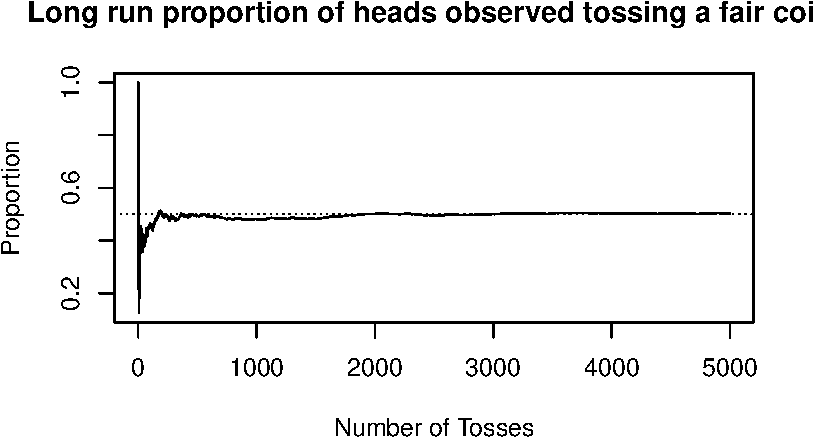
\includegraphics[keepaspectratio]{notes/chapter1_files/figure-pdf/fig-plot-1.pdf}}

}

\end{figure}%

To formalize this mathematically, we first define several important
terms.

\begin{definition}[Experiment]\protect\hypertarget{def-experiment}{}\label{def-experiment}

Any action to be performed whose outcome is not (or cannot) be known
with certainty, before it is performed.

\end{definition}

\begin{definition}[Event
{[}Informally{]}]\protect\hypertarget{def-event-inf}{}\label{def-event-inf}

A specified result that may or may not occur when an experiment is
performed.

\end{definition}

Suppose that an experiment can be performed as many times as one likes,
limited only by your boredom. If you take \(k_N\) to represent the
number of times that the event of interest occurs when you perform the
experiment \(N\) times, then a Frequentist would define the probability
of the event as \[\text{probability} = \lim_{N\to\infty}\frac{k_N}{N}.\]
If you have never taken a calculus course, and thus are unfamiliar with
the concept of limits, that is not a barrier to understanding this
statement. When you see a statement of the form
\[\lim_{x\to\infty} f(x),\] simply think ``what is happening to the
function \(f(x)\) as \(x\) grows and grows (off to \(\infty\))?''

In practice this means that, in order to interpret probabilities, we
think about repeating an experiment many, many times over. As we do
that, we observe the proportion of time that any particular outcome
occurs, and take that to be the defining relation for probabilities. The
reason that we say the probability of flipping heads is \(0.5\) is
because if we were to sit around and flip a coin\footnote{Our
  experiment.} over, and over, and over again, then in the long-run we
would observe a head\footnote{Our event.} in \(0.5\) of cases.

\begin{example}[Probability
Interpretation]\protect\hypertarget{exm-prob-interp}{}\label{exm-prob-interp}

How do we interpret the statement ``the probability that Sadie would
have had to pay, given a head on the first toss, is \(0.25\)''? Recall
that in the game, they toss three coins, and Sadie pays if two of them
show tails.

\begin{tcolorbox}[enhanced jigsaw, arc=.35mm, rightrule=.15mm, breakable, bottomrule=.15mm, left=2mm, toprule=.15mm, leftrule=.75mm, opacityback=0, colback=white, colframe=quarto-callout-color-frame]

\vspace{-3mm}\textbf{Solution}\vspace{3mm}

This statement means that, if Sadie were to repeatedly be in the
situation where one head has shown and there are two coins left to toss,
then in \(0.25\) of these situations (in the limit, as this is repeated
an infinite number of times) will end up showing two tails.

\end{tcolorbox}

\end{example}

Many situations in the real world cannot be run over and over again.
Think about, for instance, the probability that a particular candidate
wins in a particular election. There is uncertainty there, of course,
but the election can only be run once. What then? There are several ways
through these types of events.

First, we can rely on the \textbf{power of imagination}. There is
nothing stopping us from envisioning the hypothetical possibility of
running the election over, and over, and over, and over again. If we
step outside of reality for a moment, we can ask ``if we could play the
day of the election many, many, many times, what proportion of those
days would end with the candidate being elected?'' If we say that the
candidate has a 75\% chance of being elected, then we mean that in
\(0.75\) of those imagined worlds, the candidate wins. It is crucial to
stress that in our imagination here, we need to be thinking about the
\textbf{exact same day} over and over again. We cannot imagine a
different path leading to the election, different speeches being given
in advance, or different opposition candidates. If we start from the
same place, and play it out many times over, what happens in each of
those worlds?

This repeated imagining is not for everyone. As a result, alternative
proposals to the interpretation of probability have been made, with the
\textbf{Bayesian interpretation} (or subjectivist interpretation) being
particularly prominent. To Bayesians, probability is a measure of
subjective belief. To say that there is a \(50\%\) chance of a coin
coming up is a statement about one's knowledge of the world. The
Bayesian view, built around subjective confidence in the state of the
world, can be formalized mathematically as well. A Bayesian considers
the \emph{prior evidence} that they have about the world\footnote{Any
  relevant evidence that has previously been collected.} and combine
this with current observations in order to update their subject beliefs,
balancing these two sources of information.

\begin{remark}[Bayesian Probabilities and Belief Updating]
Suppose that a Bayesian is flipping a coin. Before any flips have been
made the Bayesian understandably believes that the coin will come up
heads \(50\%\) of the time. However, when the coin starts to be flipped,
the observations are a string of tails in a row.

After having flipped the coin five times, the individual has observed
five tails. Of course, it is totally possible to flip a fair coin five
times and see five tails, but there is a level of skepticism growing.

After 10 flips, the Bayesian has still not seen a head. At this point,
the subjective belief is that there is likely something unfair about
this coin. Even though the experiment started with a baseline assumption
that the coin was fair the Bayesian no longer believes that the next
flip will be a head.

As this goes on, you can imagine the Bayesian continuing to update their
view of the world. To them, the probability is an evolving concept,
capturing what was believed and what has been observed.
\end{remark}

For the election example, the Bayesian interpretation is somewhat easier
to think through. To say that a candidate has a \(75\%\) chance of
winning the election means that ``based on everything that has been
observed, and any prior beliefs about the viability of the candidates,
the subjective likelihood that the candidate wins the election is
\(0.75\)''. If we disagree about prior beliefs, or have experienced
different pieces of information, then we may disagree on the
probability. That is okay.

In these notes, we focus on the Frequentist interpretation. This choice
is not a strong stance on the relative merits of the two viewpoints.
There is some research to suggest that Frequentist interpretations are
fairly well understood by the general public\footnote{See, for instance
  Gigerenzer et al. (2005), where they study how people interpret the
  statement ``there is a \(30\%\) chance of rain tomorrow.''
  Interestingly, most people can convert this into a frequency statement
  (\(3\) out of \(10\), say), even if the specific meaning is sometimes
  lost. They conclude that there are other issues in attempting to
  understanding this statement, issues which we will address later on.}.
However, it is important to know and recognize that there is a world
beyond Frequentist Probability and Statistics, one which is very
powerful once it is unlocked.\footnote{More on this in later books, if
  you so desire!}

If probability measures the long term proportion of time that a
particular event occurs, how can we go about computing probabilities? Do
we require performing an experiment over and over again? Fortunately,
the answer is no. The tools of probability we will cover allow us to
make concrete statements about the probabilities of events without the
need for repeated experimental runs. However, before completely
dismissing the idea of repeatedly running an experiment, it is worth
considering a tool we have at our disposal that renders this more
possible than it has ever been: computers.

\section{R Programming for Probability and
Statistics}\label{r-programming-for-probability-and-statistics}

Throughout these notes we will make use of a programming language for
statistical computing, called R. Classically, introductory statistics
courses involved heavy computation of particular quantities by hand. The
use of a programming language (like R) frees us from the tedium of these
calculations, allowing for a deeper focus on understanding, explanation,
decision-making, and complex problem-solving. This is \textbf{not} to
say we will \emph{never} do problems by hand\footnote{To the contrary,
  some amount of by-hand problem-solving helps to solidify these
  concepts.}, however, these notes emphasize the use of statistical
computing. The sections on R programming throughout the notes are
self-contained, and separate from the main material. Studying these
sections will give you familiarity and comfort with reading, modifying,
and writing R scripts for statistical programming.

It may be useful to have R open alongside the notes to ensure that you
can get the same results that are printed throughout. In this section we
will cover the very basics of using R, and reading R code. If you are
interested, there are plenty of resources to becoming a more proficient
R programmer.

\subsection{Basic Introduction to R
Programming}\label{basic-introduction-to-r-programming}

When programming, the basic idea is that we are going to write
instructions in a \textbf{script} which we will tell our computer to
execute. These instructions are\footnote{Typically. There are some
  exceptions to this, but if this is your first time programming, you
  need not worry about that!} performed one-by-one, from the top to the
bottom of the script. We can have instructions which operate on their
own, or which interact with previous (or future) instructions to add to
the complexity. The trick with programming then is to determine which
actions you need the computer to perform, in which order, to accomplish
the task that you are setting out to do.

To begin, we may consider an R program that uses the programming
language as a basic calculator.

\begin{verbatim}
## [1] 33554420
\end{verbatim}

Here, we ask the computer to perform arithmetic operations. We use
\texttt{+} for addition, \texttt{-} for subtraction, \texttt{*} for
multiplication, \texttt{/} for division, and \texttt{\^{}} for
exponentiation. With the use of parentheses, any expressions relating to
these basic operations can be performed. Note that here the result is
output after it is computed. Try modifying the exact expressions being
computed, allowing you to feel comfortable with these types of
mathematical operations.

\begin{verbatim}
## [1] 33554420
## [1] 40
\end{verbatim}

Here, we have two lines of math running with arithmetic operations. Each
is output when it is computed. These two results have no ability to
interact with one another, and if we were to add more and more lines
beneath, the same would continue to happen.

If we want different commands to be able to interact with one another,
we need a method for storing the results. To do so, we can define
\textbf{variables}. In R, to define a variable, we use the syntax
\texttt{variable\_name\ \textless{}-\ variable\_value}. We can choose
\emph{almost} anything that we want for the variable name\footnote{The
  variable name must start with a letter and can be a combination of
  letters, numbers, periods, and underscores.} and the variable value
can also be of many types.\footnote{more on this later} The arrow
between the two is the \textbf{assignment operator}. It tells R to
assign the \texttt{variable\_value} to be accessible from the
\texttt{variable\_name}.

\begin{verbatim}
## [1] 5
## [1] 8
\end{verbatim}

In this code we assign the variable \texttt{my\_5} to contain the value
5, and the variable \texttt{my\_8} to contain the value 8. We can output
these as expressions themselves by typing the variable name. Directly
outputting these variables is not of particular interest, however, we
can use the variables in later statements by including the variable name
in them.

\begin{verbatim}
## [1] 40
\end{verbatim}

Here, instead of outputting the variables, we multiply them together. We
could have used \texttt{5\ *\ 8} in this case for the same result,
however, we are afforded a lot more flexibility with this approach. Much
of this flexibility comes from our capacity to \emph{change} the values
of variables over time. Consider the following script, and try to
understand why the output is the way that it is.

\begin{verbatim}
## [1] 40
## [1] 80
\end{verbatim}

At the top point in the script, before the first \texttt{my\_5*my\_8}
call, the variable \texttt{my\_5} has the value \texttt{5}. However,
after this is called, the value is updated to be \texttt{10}. Then, when
we call \texttt{my\_5*my\_8} again, this is now simplified to
\texttt{10\ *\ 8}, giving the result. Perhaps more importantly, we can
take the value of an expression and assign that to a variable itself.

\begin{verbatim}
## [1] 40
\end{verbatim}

Here, we define another variable. This time, \texttt{result} now
contains the result of multiplying our previous two variables. Thus,
when we output it, we get the same value. Take a moment to read through
the following script, and try to understand what will happen at the end.

The result is 1600. Why? We can read through this step-by-step in order
to understand this. First we set our variables to have the values of
\texttt{5} and \texttt{8}. Then, \texttt{result} is made to be the
product of our two variables, which in this case is \texttt{40}. After
that, we set the value of \texttt{my\_5} to be the same as the value of
\texttt{result}, which gives \texttt{my\_5} equal to \texttt{40}. At
this point, \texttt{result} equals \texttt{40}, \texttt{my\_5} equals
\texttt{40}, and \texttt{my\_8} is equal to \texttt{8}. The next line
updates \texttt{my\_8} to be the same as the value of \texttt{my\_5},
which we just clarified was \texttt{40}. As a result, all the variables
we have defined now take on the value of \texttt{40}. The final line
before output, \texttt{result\ \textless{}-\ my\_5\ *\ my\_8} updates
the value of \texttt{result} to be the product of the two variables
again, this time giving \texttt{40\ *\ 40} which gives 1600.

\subsection{Function Calls in R}\label{function-calls-in-r}

Up until this point we have only used numerical operations and variable
assignment. While this allows R to serve as a very powerful calculator,
we often want computers to do much more than arithmetic. As a result, we
need to explore \textbf{functions} in R. A function is a piece of code
which takes in various arguments and outputs some value (or values).
Most of the way that we will use R in these notes is through the use of
function calls.\footnote{Note: when you begin to write programs for
  yourself, a lot of your time will be spent writing custom functions.
  If this is of interest to you, I suggest looking into programming
  more! For now, we will not need to define our own functions.} This is
exactly analogous to a mathematical function: it is some rule which maps
input to output. In fact, some of the most basic functions in R are
functions which relate to mathematical functions.

\begin{verbatim}
## [1] 22026.47
## [1] 3.162278
## [1] 2.302585
\end{verbatim}

\begin{enumerate}
\def\labelenumi{\arabic{enumi}.}
\tightlist
\item
  Computes the exponential function applied to \texttt{x}, that is
  \(e^x = e^{10}\).
\item
  Computes the square root of \texttt{x}, that is
  \(\sqrt{x} = \sqrt{10}\).
\item
  Computes the natural logarithm of \texttt{x}, that is
  \(\log(x) = \log(10)\).
\end{enumerate}

The basic format of a function call will always be
\texttt{function\_name(param1,\ param2,\ ...)}. Each of these functions
required only a single parameter, however, there are some functions
which take more than one parameter. If we have decimal numbers, for
instance, we may wish to round them. To do so, we can use the
\texttt{round} function in R, which takes two parameters: the number we
wish to round, and how many digits we wish to keep.

\begin{verbatim}
## [1] 3.142
\end{verbatim}

There are a few things to note about this sequence of function calls.
First, notice that we assign the output of a function to a new variable.
This behaves exactly as we saw above with numeric calculations. Next,
consider that the output of the function\footnote{Which we have stored
  in the variable \texttt{rounded\_value}} has a value of \(3.142\).
That is: we rounded the value to \(3\) decimal points, exactly as would
be expected. Finally, notice that the second parameter passed to the
function call is \textbf{named}. That is, instead of calling
\texttt{round(unrounded\_value,\ 3)}, we have
\texttt{round(unrounded\_value,\ digits\ =\ 3)}. If you had made the
first call this would have worked perfectly.\footnote{Try it out to
  convince yourself!} However, R also provides the ability to pass in
parameter names alongside the parameter values with the syntax
\texttt{function\_name(param\_name\ =\ param\_value,\ ...)}.

The benefit to doing this is two-fold. First, it is easier to read what
is happening, especially for function calls that you have never seen
before. Second, it removes the need to have the parameters ordered
correctly. It is best practice to \textbf{always} include parameter
names where you can.

Now, you may be wondering ``how do you know what the parameter names
should be?'' The names are built-in to the different functions that you
are working with, and with experience you will become quite familiar
with them. However, at any point you can also run the command
\texttt{?function\_name}, replacing \texttt{function\_name} with the
name of a function you are interested in, to open documentation about
that function. There you will see not only the names of the different
parameters, but useful information regarding what the function does, and
examples of how to call it.

When we run this code, we are given \emph{a lot} of information. We can
see the function name, the details, how it's called, and so forth. In
the \textbf{Arguments} section we get a list of all the arguments we can
pass to the function, along with a description of them. In this case we
see that \texttt{round} can take a parameter called \texttt{x} for the
number to be rounded, and \texttt{digits} (which we have previously
seen).

\begin{verbatim}
## [1] 3.142
\end{verbatim}

This code produces the exact same output, where now both parameters are
named. Specifically, we could read this function call as ``round the
value of \texttt{x} to have \texttt{digits} decimal points.'' If you had
instead written \texttt{round(3,\ unrounded\_value)}, you would get the
value \texttt{3}, since now we are rounding \texttt{3} to
\texttt{3.141592} decimal points.

\subsection{Moving Beyond Numeric
Data}\label{moving-beyond-numeric-data}

So far, everything that we have looked at has been numeric data. We have
seen integers, and decimals. You can have negative results, say by
taking \texttt{my\_var\ \textless{}-\ -5}. And while numbers are
frequently useful, we will require further types of data to write useful
computer programs. In these notes, we will focus on three additional
data types: textual data which (referred to as \textbf{strings}), true
and false binary data (referred to as \textbf{logicals} in R), and lists
of the same data type (referred to as \textbf{vectors}). They will
behave in much the same way as numeric data, with different functions
and techniques which can be applied to them.

To define a string of text, we encapsulate the text that we are
interested in within quotation marks (either single
\texttt{\textquotesingle{}} or double \texttt{"} quotation marks will
work).

\begin{verbatim}
## [1] "This is a string."
\end{verbatim}

Two commonly used functions which rely on strings are \texttt{paste} and
\texttt{print}. Each will take in strings as input, and they do not need
to be named. The function \texttt{paste} can take in as many strings as
you would like. It will ``paste'' together all the strings provided,
creating a longer string out of these. The function \texttt{print} will
display the string that is passed as output. Until now, we have been
running these programs in a way where all calls are displayed as output:
this will not always be the case, and so print can come in handy there.

\begin{verbatim}
## [1] "Hello! Welcome to R programming, Dylan !"
\end{verbatim}

Note that \texttt{paste} has several additional options which can be
investigated in the documentation. This is only the simplest use case
for it. In general, strings are particularly helpful when we wish to
have output from the computer that will be human-readable. Where strings
are largely for humans, logicals are largely for computers.

Much of what computer programming entails is checking whether certain
conditions hold, and then taking different actions depending on what is
found. In order to do this, the computer needs a way to represent true
and false statements. In R, these are codified with the values
\texttt{TRUE} and \texttt{FALSE}. Note, the capital letters here make a
difference. You cannot use \texttt{true} or \texttt{True} or any other
combination thereof. More important than being able to specify the
values \texttt{TRUE} and \texttt{FALSE} directly is the ability to
detect whether certain statements are \texttt{TRUE} or \texttt{FALSE}.
For this we require comparison operators.

If we think of mathematical comparisons we can state whether two things
are equal, or not equal, and whether one thing is less than (or equal
to) or greater than (or equal to) another. We can run all of these same
checks in R.

\begin{itemize}
\tightlist
\item
  To check whether two quantities are equal you use
  \texttt{quantity\_1\ ==\ quantity\_2}. This statement will be
  \texttt{TRUE} if \texttt{quantity\_1} and \texttt{quantity\_2} are
  exactly the same, and will be \texttt{FALSE} otherwise.
\item
  To check whether two quantities are not equal, you can use
  \texttt{quantity\_1\ !=\ quantity\_2}. This statement will be
  \texttt{TRUE} if the quantities differ from one another.
\item
  To check whether one quantity is larger than another, you can use
  \texttt{quantity\_1\ \textgreater{}\ quantity\_2}. If you want to know
  whether it is greater than \emph{or} equal to, you can use
  \texttt{quantity\_1\ \textgreater{}=\ quantity\_2}.
\item
  To check whether one quantity is smaller than another, you can use
  \texttt{quantity\_1\ \textless{}\ quantity\_2}. If you want to know
  whether it is less than \emph{or} equal to, you can use
  \texttt{quantity\_1\ \textless{}=\ quantity\_2}.
\end{itemize}

\begin{verbatim}
## [1] TRUE
## [1] FALSE
## [1] FALSE
## [1] TRUE
## [1] FALSE
## [1] FALSE
## [1] FALSE
## [1] TRUE
## [1] TRUE
## [1] FALSE
## [1] TRUE
## [1] TRUE
\end{verbatim}

There are two key points to note beyond this. First, we will of course
not normally compare two constants to one another. We already know that
\texttt{5==5}, so we would not need to check it. We can, however,
plug-in variables, perhaps with unknown values, and have the same types
of statements being made. Second, the checks for equality and inequality
also work with other data types (like strings).

\begin{verbatim}
## [1] TRUE
## [1] FALSE
## [1] TRUE
## [1] TRUE
## [1] TRUE
## [1] FALSE
## [1] FALSE
## [1] TRUE
## [1] TRUE
## [1] FALSE
\end{verbatim}

The final checks may be slightly odd. Here we are comparing across
different types of data. When we do this R will automatically try to
convert from one type to the other. With strings and numbers this is not
too challenging. If they can be converted nicely between types, then
they are and the values are compared. Otherwise, R will conclude they
are not equal by default. For logicals, it is important to note that
\texttt{TRUE\ ==\ 1} and \texttt{FALSE\ ==\ 0}. We will often use these
values interchangeably.

The final data type that we will consider are vectors. Vectors store
multiple values, of the same type, in a single object. Thus, we may have
a vector of numeric data, or a vector of strings, or a vector of
logicals. The vectors will always contain the same type throughout, but
they are stored in a single object (and as such, for instance, can be
stored in a single variable). To define a vector we call
\texttt{c(...)}, where the \texttt{...} contains the set of objects we
want to store in the vector. The \texttt{c} stands for
\textbf{c}oncatenate, as we are \emph{concatenating} together the set of
items into a single container.

\begin{verbatim}
## [1] "vector"  "of"      "strings"
## [1] 3 1 4 1 5
## [1]  TRUE  TRUE FALSE  TRUE
## [1] FALSE  TRUE FALSE
\end{verbatim}

We see that each of these vectors holds one type of object. Vectors can
be of arbitrary and different lengths. It is also possible to combine
multiple vectors \emph{of the same type} into one, by using the
\texttt{c} function again.

\begin{verbatim}
##  [1] 3 1 4 1 5 9 2 6 5 3
\end{verbatim}

Here we combine different numeric vectors together. We also show, when
forming \texttt{combined\_v3}, how numeric vectors can have single items
added onto them. That is, if you have a single number, it can be treated
as a vector with one element in it. This becomes very useful when
building up vectors within code.

In addition to combining multiple vectors together, we can also select
elements out of a vector. To do this, we use a set of square brackets
after the vector's name, with a number within those square brackets
specifying the \textbf{index} of the vector we are interested in. The
index is the element position starting at 1\footnote{If you have
  programmed in the past there is a good chance the language you have
  learned is ``0 indexed'' rather than ``1 indexed''. In R, all vectors
  start at position 1 and count up, which is not the case in many
  languages. Be careful of this.} and running to the length of the
vector. We can include a vector of indices to select multiple elements
at once.

\begin{verbatim}
## [1] "D"
## [1] "Y"
## [1] "L"
## [1] "A"
## [1] "N"
## [1] "D" "Y" "L" "A" "N"
\end{verbatim}

Note that, each element is selectable individually, giving a single item
of that type (in this case, strings). If you select multiple of the
elements together, it will create a vector of that type (in this case, a
string vector). In addition to selecting elements in this way by their
indices, you can also update the elements in the same way.

\begin{verbatim}
## [1] 2 0 2 3
## [1] 2 0 2 4
\end{verbatim}

In this example we are changing the last element of the vector.
Sometimes we may not know how long the vector actually is, if for
instance, it is being built-up as our code runs. If we ever want to
check the length of a vector, we can call the function \texttt{length}
which takes as input only one vector, and outputs the numeric value of
its length.

\begin{verbatim}
## [1] 5
\end{verbatim}

\subsection{Program Control Flow}\label{program-control-flow}

We have seen different types of data, different ways of manipulating
data, functions, and variables so far. In order to bring all of these
concepts together into useful programs we need some way to control the
flow of our programs. We have seen that, by default, programs execute
from the top until the bottom. However, it will often be the case that
we want to have certain code running only if certain conditions hold, or
that we want to repeat some piece of code many times over. To accomplish
these tasks we require \textbf{control flow statements}. We will
consider only two types of control flow statements now, which will serve
well enough to read most of what needs to be read for these notes.

The first type of statement is the \textbf{conditional statement}.
Conditional statements execute only when certain conditions hold. The
simplest conditional statement is an \textbf{if} statement. The format
to define an if statement is \texttt{if\ (condition)\{\ ...\ \}}, where
\texttt{condition} is some logical condition to be evaluated. If the
condition is \texttt{TRUE} then the code contained in \{ \ldots{} \} is
evaluated. If the condition is \texttt{FALSE} it is not.

\begin{verbatim}
## [1] "My number is a positive."
\end{verbatim}

In this case, these conditional statement check to see whether the
number we entered is larger than zero and whether the number we entered
is smaller than zero, respectively. When run, notice that at most one of
the statements is executed.\footnote{In fact, if \texttt{my\_number} is
  set to \texttt{0} then none of the statements are executed.} In this
case, we know that only one (or neither) of these statements can be
true. When that is the case it may make sense to make use of
\texttt{else} clauses in our conditional logic.

\begin{verbatim}
## [1] "My number is not a positive."
\end{verbatim}

Here, if the number is greater than \texttt{0}, then we run the first
block of code, otherwise we run the second block of code. Thus, whenever
a positive number is entered, we see ``My number is a positive'', and
whenever a non-positive number is entered, we see ``My number is not a
positive.'' We can extend \texttt{else} blocks to be \texttt{else\ if}
blocks, where further conditions can be specified.

\begin{verbatim}
## [1] "My number is a large positive value."
\end{verbatim}

In these case we can pass through each conditional statement in order.
First, is the number larger than \texttt{50}? If so, print the
statement, otherwise we check the next condition, is the number greater
than \texttt{0}? Note that if we are checking this condition we
\emph{know} that the number is less than or equal to \texttt{50} since
it failed the first check. We continue through the rest of this
procedure down until the last else block. This block is run only when
all of the other conditions fail: that is, our value is not larger than
\texttt{50}, or larger than \texttt{0}, or smaller than \texttt{-50}, or
smaller than \texttt{0}. The only value that satisfies this is
\texttt{0} itself.

Sometimes, we wish to check compound conditions. That is, we want to
know whether multiple conditions hold, or perhaps, whether at least one
of many conditions hold. These statements can be converted into ``and''
and ``or'' statements, respectively. To denote ``and'' statements we use
\texttt{\&\&} and to denote ``or'' statements we use
\texttt{\textbar{}\textbar{}}. Thus, the check
\texttt{my\_val\ \textgreater{}\ 0\ \&\&\ my\_val\ \textless{}\ 100}
returns true only if \texttt{my\_val} is both above \texttt{0}
\textbf{and} below 100. The check
\texttt{my\_val\ \textless{}\ -50\ \textbar{}\textbar{}\ my\_val\ \textgreater{}\ 50}
returns true whenever \textbf{either} \texttt{my\_val} is less than
\texttt{-50} \textbf{or} \texttt{my\_val} is greater than \texttt{50}.

\begin{verbatim}
## [1] "Either 5 or a negative value."
\end{verbatim}

Conditional statements can grow to be very complex, however, with these
rules you can read through them top-to-bottom, substituting for ``and''
and ``or'' where necessary. It is also possible, where required, to
place one conditional statement inside the code block for another, and
to combine them with any of the other techniques that we have learned
thus far.

The final piece of control flow that we will consider for now is the
\texttt{for} loop. The idea with a \texttt{for} loop is that we want to
repeat the same action either a certain number of times, or for every
item in a set of items. To do so, we use the syntax
\texttt{for(x\ in\ vector)\{...\}}, where the code in \texttt{...} will
be performed once for every single item in the vector. Within the code
block specified by \texttt{...}, the value \texttt{x} will take on the
current value in the loop.

\begin{verbatim}
## [1] 1
## [1] 2
## [1] 3
\end{verbatim}

Notice that three values are printed, in order, \texttt{1} then
\texttt{2} then \texttt{3}. The loop code is run three different times,
one for each element in the list. Each time the loop is running the next
value from the list gets assigned to the variable \texttt{x}. The first
time it runs it gets the first element, and so forth. As a result, we
can use these values in our calculations in whatever way we need to.

\begin{verbatim}
## [1] "The square of 1 is 1"
## [1] "The square of 2 is 4"
## [1] "The square of 3 is 9"
\end{verbatim}

Whenever we are trying to form a numeric vector with consecutive
elements, as we are in \texttt{c(1,2,3)}, we can make this easier on
ourselves by specifying the upper and lower bounds of the range,
separated by a colon. That is \texttt{c(1,2,3)\ ==\ 1:3}. This is often
useful when specify a loop as we very often want to repeat something a
set number of times. Note that we do not ever \emph{need} to use the
value of the looping variable. Sometimes, we just want things to repeat,
and so the loop is a convenient way to do that.

\begin{verbatim}
## [1] "This will get printed 5 times."
## [1] "This will get printed 5 times."
## [1] "This will get printed 5 times."
## [1] "This will get printed 5 times."
## [1] "This will get printed 5 times."
\end{verbatim}

\subsection{Reading Through a More Complex R
Program}\label{reading-through-a-more-complex-r-program}

Take a moment to read through the following R program and try to
understand what is happening exactly. There are comments throughout
which will assist in the parsing of the script. We have seen comments up
until now, without drawing explicit attention to them. In R, anything
placed after a \texttt{\#} on the line is considered a comment. The
programming language ignores these and so they are only there to help
other individuals who may be reading through. It is good practice to
comment your code to help others, and also to help yourself whenever you
return to it in the future. In these notes code will typically be
commented. If you are reading the PDF version of the notes often these
comments will be annotations beside the code (numbering certain lines)
with the comments provided below, for the sake of legibility.

Note, this combines everything that we have learned, and it is entirely
understandable if it takes some time to process. Fortunately, you can
always try running the script yourself, and playing with different
components of it. Remember, if you do not know what a function call
does, you can use the documentation\footnote{The internet is also a
  wonderful resource, one which even very experienced developers make
  frequent use of.} and try playing with it some yourself. To help with
the interpretation here, note that this is an implementation of the game
that Charles and Sadie have been playing.

\begin{verbatim}
## [1] "Now starting round 1"
## [1] "The flip was a H which benefits Charles"
## [1] "Now starting round 2"
## [1] "The flip was a T which benefits Sadie"
## [1] "Now starting round 3"
## [1] "The flip was a T which benefits Sadie"
## [1] "Sadie has scored enough points to win."
## [1] "After flipping the coin 3 times, Charles scored a total of 1 points"
## [1] "while Sadie scored a total of 2 points."
## [1] "As a result Sadie won the game and will not have to pay!"
\end{verbatim}

\subsection{R Programming for Probability
Interpretations}\label{r-programming-for-probability-interpretations}

Recall that the motivation for the discussion of R was the Frequentist
interpretation of probability. Computers are very effective at
repeatedly performing some action. As a result, we can use computers to
mimic the idea of repeatedly performing an experiment. Consider the case
of flipping a coin over and over again.

We can use \texttt{sample(x,\ size)} as a function to select
\texttt{size} realizations from the set contained in \texttt{x}. Thus,
if we take \texttt{sample(x\ =\ c("H","T"),\ size=1)} we can view this
as flipping a coin one time. If we use the loop structure we talked
before, then we can simulate the experience of repeatedly flipping a
coin. Consider the following R code. Note, any time that we are doing
something which is randomized in R (such as drawing random samples) we
also will make use of the \texttt{set.seed()} function. This function
takes in an integer value as an argument, and by providing the
\emph{same} integer value we can make sure to always get the same random
numbers generated.\footnote{Technically, we cannot use a computer to
  generate random numbers. We can only generate \emph{pseudo random}
  numbers, which are close enough for most purposes.} This helps to
ensure the repeatability of any R analysis, and it is good practice to
do. To see what happens without seeding, try modifying the following
code without a seed, and running it several times. Then, set the seed
(to any number you like) and do the same process.

\begin{verbatim}
## [1] 0.522
\end{verbatim}

\begin{enumerate}
\def\labelenumi{\arabic{enumi}.}
\tightlist
\item
  A seed ensures that the random numbers generated by the program are
  always the same. This helps to be able to reproduce our work.
\item
  This is how many times we want to repeat the experiment.
\item
  This is where we are going to store the results of our tosses. It
  creates an empty list for us.
\item
  Here we are going to loop over the experiments, one for each run.
\item
  This is our coin toss. We are going to sample 1 from either `H' or `T'
\item
  If the coin toss is heads, then we add a 1 to the list. Otherwise, we
  add a zero to the list.
\item
  Return the mean of all of the tosses.
\end{enumerate}

It is worth adjusting some of the parameters within the simulation, and
seeing what happens. What if you ran the experiment only 5 times? Ten
thousand times? What if instead of counting the number of heads, we
wanted to count the number of tails? What if we wanted to count the
number of times that a six-sided die rolled a 4? All of these settings
can be investigated with modifications to the provided script.

\subsection*{References}\label{references-1}
\addcontentsline{toc}{subsection}{References}

\chapter{The Mathematical Foundations of Statistical
Experiments}\label{the-mathematical-foundations-of-statistical-experiments}

\section{The Sample Space and Events}\label{the-sample-space-and-events}

In Chapter 1 we saw the mathematical formulation for the Frequentist
interpretation of probability. To study probability, we require a more
detailed mathematical model. We want a description, framed in terms of
mathematical objects, which will allow us to work out probabilities of
interest. In general, to form such a probability model we need both a
list of all possible outcomes that the experiment can produce, as well
as the probabilities of these outcomes.

We call the list of outcomes that can occur from an experiment the
\textbf{sample space} of the experiment. The sample space is denoted
\(\mathcal{S}\), and is defined as the set of all possible outcomes from
the experiment. For instance, if the experiment is flipping a coin we
have \(\mathcal{S} = \{\text{H}, \text{T}\}\). If the experiment is
rolling a six-sided die then \(\mathcal{S} = \{1,2,3,4,5,6\}\).

\begin{definition}[Sample
Space]\protect\hypertarget{def-sample-space}{}\label{def-sample-space}

The sample space of a statistical experiment is the set of all possible
outcomes that can be realized from that experiment. The sample space is
typically denoted \(\mathcal{S}\), or with similar script letters.

\end{definition}

\begin{example}[Enumerating Sample
Spaces]\protect\hypertarget{exm-sample-space-basic}{}\label{exm-sample-space-basic}

Write down the complete sample space, \(\mathcal{S}\) for the game that
Sadie and Charles play, based on flipping and observing a coin three
times in sequence.

\begin{tcolorbox}[enhanced jigsaw, arc=.35mm, rightrule=.15mm, breakable, bottomrule=.15mm, left=2mm, toprule=.15mm, leftrule=.75mm, opacityback=0, colback=white, colframe=quarto-callout-color-frame]

\vspace{-3mm}\textbf{Solution}\vspace{3mm}

For Sadie and Charles their experiment involves tossing a coin three
times in sequence. As a result each outcome is a three-dimensional list
of values, given for instance by \((\text{H},\text{H},\text{H})\). We
can write the full sample space as
\[\mathcal{S} = \{(\text{H},\text{H},\text{H}), (\text{H},\text{H},\text{T}), (\text{H},\text{T},\text{H}), (\text{H},\text{T},\text{T}), (\text{T},\text{H},\text{H}), (\text{T},\text{H},\text{T}), (\text{T},\text{T},\text{H}), (\text{T},\text{T},\text{T})\}.\]

\end{tcolorbox}

\end{example}

With the sample space formally defined, we can revisit
Definition~\ref{def-event-inf}, and formally define the concept of an
event.

\begin{definition}[Event]\protect\hypertarget{def-event}{}\label{def-event}

An event is any collection of outcomes from a sample space for a
statistical experiment. Mathematically, an event, \(E\), is a subset of
\(\mathcal{S}\), and we write \(E\subset\mathcal{S}\).

\end{definition}

Take for instance the experiment of a single coin. In this case, we may
define \(E_1 = \{\text{H}\}\), \(E_2 = \{\text{T}\}\), and
\(E_3 = \{\text{H},\text{T}\}\) as examples of possible events. Here,
\(E_1\) corresponds to the event that a head is observed, \(E_2\)
corresponds to the event that a tail is observed, and \(E_3\)
corresponds to the event that either a tails or a heads was observed.
Note that for each event we have \(E_1 \subseteq\mathcal{S}\),
\(E_2 \subseteq\mathcal{S}\), and
\(E_3 \subseteq \mathcal{S}\).\footnote{Note that the symbol
  \(\subseteq\) is the \emph{subset or equal} symbol. If we write
  \(A \subseteq B\), then \(A\) is either a subset of \(B\) or else
  \(A\) is equal to \(B\). This is in contrast to using \(A \subseteqB\)
  which suggests that \(A\) is not equal to \(B\). The distinction is
  analogous to the difference between writing \(x < y\) versus
  \(x \leq y\). Throughout these notes we will predominantly use
  \(\subseteq\).}

\begin{example}[Basic Event
Listing]\protect\hypertarget{exm-basic-events}{}\label{exm-basic-events}

List several events from the game that Charles and Sadie are playing.
Indicate why these are events.

\begin{tcolorbox}[enhanced jigsaw, arc=.35mm, rightrule=.15mm, breakable, bottomrule=.15mm, left=2mm, toprule=.15mm, leftrule=.75mm, opacityback=0, colback=white, colframe=quarto-callout-color-frame]

\vspace{-3mm}\textbf{Solution}\vspace{3mm}

Recall that an event is any subset of the sample space. In
Example~\ref{exm-sample-space-basic} we define \(\mathcal{S}\) for this
game. As a result we can take sets which contain any combinations of
these elements. For instance \(E_1 = \{(\text{H},\text{H},\text{H})\}\),
or
\(E_2 = \{(\text{H},\text{H},\text{T}), (\text{H},\text{T},\text{H})\}\),
or
\[E_3 = \{(\text{H},\text{H},\text{H}), (\text{H},\text{H},\text{T}), (\text{H},\text{T},\text{H}), (\text{H},\text{T},\text{T}), (\text{T},\text{H},\text{H}), (\text{T},\text{H},\text{T}), (\text{T},\text{T},\text{H}), (\text{T},\text{T},\text{T})\}.\]
These are all events since \(E_1 \subseteq\mathcal{S}\),
\(E_2 \subseteq\mathcal{S}\), and \(E_3 \subseteq\mathcal{S}\).

\end{tcolorbox}

\end{example}

\begin{example}[Event
Identification]\protect\hypertarget{exm-event-identification}{}\label{exm-event-identification}

Is ``Charles has to pay'' an event from the game that Charles and Sadie
are playing? Why? Explain.

\begin{tcolorbox}[enhanced jigsaw, arc=.35mm, rightrule=.15mm, breakable, bottomrule=.15mm, left=2mm, toprule=.15mm, leftrule=.75mm, opacityback=0, colback=white, colframe=quarto-callout-color-frame]

\vspace{-3mm}\textbf{Solution}\vspace{3mm}

``Charles has to pay'' is not directly an event, as it is not a subset
of the sample space. This could plausibly be seen as a real-world
description of a possible event, but it is not \emph{itself} an event.
The strictness of this language will be relaxed as time goes on,
however, it is important to familiarize yourself with how descriptions
are converted to events. In this case, we could take an event to be
\[E = \{(\text{H},\text{H},\text{H}), (\text{H},\text{H},\text{T}), (\text{H},\text{T},\text{H}), (\text{T},\text{H},\text{H})\},\]
and state that if \(E\) occurs then Charles has to pay.\footnotemark{}

\end{tcolorbox}

\footnotetext{When speaking to a statistician, they would understand
``Charles has to pay'' as an event that \emph{can} occur based on the
defined sample space, by simply transforming it into the language of the
sample space. However, the distinction is important to make: events are
always subsets of the sample space. Once this is second nature, it is a
rule that can be loosened, as the knowledge can always be fallen back on
when needed. Simply put: you need to know the rules in order to break
them!}

\end{example}

\begin{example}[Defining Events from Real-World
Descriptions]\protect\hypertarget{exm-event-conversion}{}\label{exm-event-conversion}

What event corresponds to the description ``Sadie has to pay'' in the
game that Charles and Sadie are playing? Recall that they flip a coin
three times, and Charles will pay if at least two heads come up, while
Sadie will pay if at least two tails come up.

\begin{tcolorbox}[enhanced jigsaw, arc=.35mm, rightrule=.15mm, breakable, bottomrule=.15mm, left=2mm, toprule=.15mm, leftrule=.75mm, opacityback=0, colback=white, colframe=quarto-callout-color-frame]

\vspace{-3mm}\textbf{Solution}\vspace{3mm}

Sadie will have to pay whenever there are two or more tails. As a result
we can enumerate the possible outcomes that leads to Sadie paying. We
have

\begin{enumerate}
\def\labelenumi{\arabic{enumi}.}
\tightlist
\item
  \((\text{T},\text{T},\text{T})\);
\item
  \((\text{H},\text{T},\text{T})\);
\item
  \((\text{T},\text{H},\text{T})\);
\item
  \((\text{T},\text{T},\text{H})\).
\end{enumerate}

Any other outcome will have fewer than two tails, and as a result, Sadie
will not have to pay. Thus, to form an event, we consider the set with
each of these outcomes in it. This gives
\[E = \{(\text{T},\text{T},\text{T}), (\text{H},\text{T},\text{T}), (\text{T},\text{H},\text{T}), (\text{T},\text{T},\text{H})\}.\]

\end{tcolorbox}

\end{example}

While the events \(E_1 = \{\text{H}\}\) and \(E_2 = \{\text{T}\}\) each
correspond to a simple outcome from the sample space,
\(E_3 = \{\text{H},\text{T}\}\) corresponds to a combined event. We call
direct outcomes \textbf{simple events} and more complex outcomes like
\(E_3\) \textbf{compound events}.

\begin{definition}[Simple
Event]\protect\hypertarget{def-simple-event}{}\label{def-simple-event}

A simple event is any event which corresponds to exactly one outcome
from the sample space. A simple event only has one way of occurring. The
size of the set for a simple event will be \(1\). The sample space, in
turn, is made up of a collection of simple events.

\end{definition}

\begin{definition}[Compound
Event]\protect\hypertarget{def-compound-event}{}\label{def-compound-event}

A compound event is any event which corresponds to more than one outcome
from the sample space. A compound event can occur in multiple different
ways. The size of the set for the compound event will be greater than
\(1\).

\end{definition}

If we consider rolling a six-sided die, then an example of a simple
event is that a four shows up, denoted \(\{4\}\). A compound event could
be that an even number is rolled, \(\{2,4,6\}\), or that a number
greater than or equal to four is rolled, \(\{4, 5, 6\}\).

\begin{example}[Identifying Simple and Compound
Events]\protect\hypertarget{exm-simple-versus-compound}{}\label{exm-simple-versus-compound}

List an example of (at least) one simple and one compound event from the
game that Charles and Sadie are playing.

\begin{tcolorbox}[enhanced jigsaw, arc=.35mm, rightrule=.15mm, breakable, bottomrule=.15mm, left=2mm, toprule=.15mm, leftrule=.75mm, opacityback=0, colback=white, colframe=quarto-callout-color-frame]

\vspace{-3mm}\textbf{Solution}\vspace{3mm}

An example of a simple event would be
\(E_1 = \{(\text{H},\text{H},\text{H})\}\) since it is comprised of
exactly one outcome. If three heads are rolled, this event occurs, there
is no other way for it to occur. An example of a compound event would be
\[E_2 = \{(\text{H},\text{H},\text{H}), (\text{T},\text{H},\text{H}), (\text{H},\text{T},\text{H}), (\text{H},\text{H},\text{T})\}.\]
Here there are four outcomes that correspond to this event, and if any
of those outcomes are observed the event occurs.

\end{tcolorbox}

\end{example}

We say that an event ``occurs'' if any of the outcomes comprising the
event occur. As a result we can have more than one event occurring as
the result of a run of a statistical experiment. Suppose that we are
rolling a fair, six-sided die. Consider the events ``an even number was
rolled'' and ``a number greater than or equal to four was rolled.'' If a
four or a six are rolled, both of these events happen simultaneously.
Our goal when working with probability will be to assign probability
values to different events. We will talk about how likely, or unlikely,
events of interest are, given the underlying statistical experiment.

Above, we defined \(E_3\) to be equal to \(\mathcal{S}\). As a result,
we can say that \(\mathcal{S}\) \emph{is} an event since
\(\mathcal{S} \subseteq \mathcal{S}\). This is the event that any
outcome is observed, which is certain to happen. Since it is certain to
happen, we know it happens with probability \(1\). There is another
``special'' event which is important to consider. We call this the
\emph{null event}. Denoted \(\emptyset\), the null event is an event
that corresponds to ``nothing in the sample space''. We know that every
time an experiment is run something in the sample space occurs, and so
the null event is assigned probability zero.

\begin{definition}[Null
Event]\protect\hypertarget{def-null-event}{}\label{def-null-event}

The null event, denoted \(\emptyset\) or \(\{\}\), is an event from a
statistical experiment which corresponds to nothing within the sample
space. The null event has probability zero, and it is impossible to
observe. Note that, no matter the sample space,
\(\emptyset\subset\mathcal{S}\).

\end{definition}

\section{Set Operations for Event
Manipulation}\label{set-operations-for-event-manipulation}

Ultimately, all events are sets. These sets are subsets of the sample
space, and can contain single or multiple outcomes. Every quantity that
we are interested in can be expressed as some set of outcomes of
interest. In building up these sets it is common to construct them
through the use of ``and'', ``or'', and ``not'' statements. That is, we
may say that our event occurs if some outcome \textbf{OR} another
outcome occurs, or perhaps our outcomes occurs if some outcome does
\textbf{NOT} occur.\footnote{While both \emph{or} and \emph{not}
  language is likely clear from the examples we have seen so far,
  \emph{and} language may be slightly less obvious. While we will
  explore this in more depth shortly, note that you could not have two
  simple events occurring simultaneously. If \(E_1\) and \(E_2\) are
  both simple events, then you can have \(E_1\) \textbf{or} \(E_2\), and
  you can have \textbf{not} \(E_1\), but you cannot have \(E_1\)
  \textbf{and} \(E_2\). This is \emph{not} true for compound events.}

Consider the example of drawing cards from a standard 52-card deck. In
such a deck there are 13 card ranks, and four card suits, with one of
each combination present. If we draw a single card we can think of the
outcomes of the experiment as being any of the 52 possible combinations
of rank and suit. We are often interested in an event such as ``the card
is red'', which is the same as saying ``the card is a heart \textbf{or}
the card is a diamond.'' Perhaps we want to know whether the card was an
ace through ten, this is the same as saying ``the card is \textbf{not} a
Jack \textbf{or} a Queen \textbf{or} a King.'' If we are interested in
the event that the ace of spades was drawn, this can be expressed by
saying that ``the card was a spade \textbf{and} the card was an ace.''

As you begin to pay attention to the linguistic representation of events
that we use, you will notice more and more the use of these words to
form compound events in particular. As a result, we give each of them a
mathematical operation which allow us to quickly and compactly express
these quantities in notation.

\begin{example}[Description of
Events]\protect\hypertarget{exm-linguistic-description}{}\label{exm-linguistic-description}

Describe ``Charles has to pay'', based on the game Charles and Sadie are
playing, using language revolving around ``or'', ``and'', and ``not''
each. That is, describe observing at least two heads, on three flips of
a coin, one time using ``or'', one time using ``and'', and one time
using ``not''.\footnote{It may be helpful to notice that you can mix and
  match these terms to your hearts content!}

\begin{tcolorbox}[enhanced jigsaw, arc=.35mm, rightrule=.15mm, breakable, bottomrule=.15mm, left=2mm, toprule=.15mm, leftrule=.75mm, opacityback=0, colback=white, colframe=quarto-callout-color-frame]

\vspace{-3mm}\textbf{Solution}\vspace{3mm}

There are many possible ways of doing so. Consider the following:

\begin{enumerate}
\def\labelenumi{\arabic{enumi}.}
\tightlist
\item
  \textbf{OR}: Two heads are observed OR three heads are observed.
\item
  \textbf{AND}: Not two tails are observed AND not three tails are
  observed.
\item
  \textbf{NOT}: Not more than one tails are observed.
\end{enumerate}

\end{tcolorbox}

\end{example}

We define mathematical operations to encapsulate the use of \textbf{or},
\textbf{and}, and \textbf{not}. These operations apply to any
mathematical sets, whether they refer to events or not.

\begin{definition}[Union]\protect\hypertarget{def-union}{}\label{def-union}

The union encodes the use of ``or'' in reference to two or more sets.
Formally, with two sets \(A\) and \(B\), the union of \(A\) and \(B\) is
the set of all elements that are contained in \(A\), or \(B\), or both
\(A\) and \(B\). We write \(A \cup B\) and read that as \(A\) union
\(B\). When we wish to take the union of many sets,
\(A_1,A_2,\dots,A_n\), we write this as
\[A_1 \cup A_2 \cup \cdots \cup A_n = \bigcup_{i=1}^n A_i.\]

\end{definition}

\begin{definition}[Intersection]\protect\hypertarget{def-intersection}{}\label{def-intersection}

The intersection captures the use of ``and'' in reference to two or more
sets. Formally, the intersection of two sets, \(A\), and \(B\), is the
set that contains all elements that belong to both \(A\) and \(B\). We
write \(A \cap B\), and say ``\(A\) intersect \(B\).'' When we wish to
take the intersection of many sets, \(A_1,A_2,\dots,A_n\), we write
\[A_1 \cap A_2 \cap \cdots \cap A_n = \bigcap_{i=1}^n A_i.\]

\end{definition}

\begin{definition}[Complement]\protect\hypertarget{def-complement}{}\label{def-complement}

The complement makes formal the concept of ``not.'' The complement of a
set is the set of all elements which occur in the sample space but are
not in the given set. We write this as \(A^C\) and say ``\(A\)
complement.'' When dealing with a sample space, \(\mathcal{S}\), the
complement of \(A\) is the set of all elements in \(\mathcal{S}\) that
are not in \(A\).

\end{definition}

\begin{example}[Basic Set
Operations]\protect\hypertarget{exm-basic-set-operations}{}\label{exm-basic-set-operations}

For the game being played by Charles and Sadie, take
\(E_1 = \{(\text{H}, \text{H}, \text{H})\}\),
\(E_2 = \{(\text{H}, \text{H}, \text{H}), (\text{T}, \text{H}, \text{H}), (\text{H}, \text{T}, \text{H})\}\),
and \(E_3 = \{(\text{H}, \text{H}, \text{T})\}\). Express the following
events.

\begin{enumerate}
\def\labelenumi{\alph{enumi}.}
\tightlist
\item
  \(E_1 \cup E_2\);
\item
  \(E_1 \cap E_2\);
\item
  \(E_2^C\);
\item
  \(E_2 \cap E_3\);
\item
  \(E_1 \cup E_2 \cup E_3\).
\end{enumerate}

\begin{tcolorbox}[enhanced jigsaw, arc=.35mm, rightrule=.15mm, breakable, bottomrule=.15mm, left=2mm, toprule=.15mm, leftrule=.75mm, opacityback=0, colback=white, colframe=quarto-callout-color-frame]

\vspace{-3mm}\textbf{Solution}\vspace{3mm}

Directly from definitions we can write down each of the following sets:

\begin{enumerate}
\def\labelenumi{\alph{enumi}.}
\tightlist
\item
  \[E_1 \cup E_2 =  \{(\text{H}, \text{H}, \text{H}), (\text{T}, \text{H}, \text{H}), (\text{H}, \text{T}, \text{H})\} = E_2.\]
  As a result, the union of \(E_1\) and \(E_2\) is simply
  \(E_2\).\footnotemark{}
\item
  \[E_1 \cap E_2 = \{(\text{H}, \text{H}, \text{H})\} = E_1.\] As a
  result, the intersection of \(E_1\) and \(E_2\) is simply
  \(E_1\).\footnotemark{}
\item
  \[E_2^C =  \{(\text{H},\text{H},\text{T}), (\text{H},\text{T},\text{T}), (\text{T},\text{H},\text{T}), (\text{T},\text{T},\text{H}), (\text{T},\text{T},\text{T})\}.\]
\item
  For \(E_2\cap E_3\) note that they share no elements. As a result, the
  intersection will be empty since there are no elements common to both
  of them. This gives \(E_2\cap E_3 = \emptyset\).
\item
  \[E_1 \cup E_2 \cup E_3 = \{(\text{H}, \text{H}, \text{H}), (\text{T}, \text{H}, \text{H}), (\text{H}, \text{T}, \text{H}), (\text{H}, \text{H}, \text{T})\}.\]
\end{enumerate}

\end{tcolorbox}

\footnotetext{Note that whenever we have two events, \(A\) and \(B\),
with \(A\subseteqB\), then \(A\cup B = B\).}

\footnotetext{Note that whenever we have two events, \(A\) and \(B\),
with \(A\subseteqB\) then \(A \cap B = A\).}

\end{example}

\begin{definition}[Disjoint
Events]\protect\hypertarget{def-disjoint-events}{}\label{def-disjoint-events}

Two events, \(E_1\) and \(E_2\) are said to be disjoint whenever their
intersection is the null event. That is, if \(E_1 \cap E_2 = \emptyset\)
then \(E_1\) and \(E_2\) are disjoint events.

\end{definition}

These concepts allow us to more compactly express sets of interest, and
in particular, will be quite useful when it comes to assigning
probability. The more times you work with the set operations, the more
familiar they will become, and as a result, practice is always useful.

Consider rolling a 6-sided die, and take \(A\) to be the event that a
\(6\) is rolled, \(B\) to be the event that the roll was at least \(5\),
\(C\) to be the event that the roll was less than \(4\), and \(D\) to be
the event that the roll was odd.

\begin{itemize}
\tightlist
\item
  If we consider \(D^C\) this is the event that the roll was even;
\item
  \(A \cup C\) is the event that a \(6\) was rolled or that a number
  less than \(4\) was rolled, which is to say anything other than a
  \(4\) or a \(5\), which we may also express as \(\{4,5\}^C\).
\item
  If we take \(A \cup B\) then this will be the same as \(B\), and
  \(A\cap B\) will be \(A\).
\item
  If we take the event \(A\cap C\), notice that no outcomes satisfy both
  conditions, and so \(A \cap C = \emptyset\).
\item
  We can also join together multiple operations. \(D^C \cap C\) gives us
  even numbers than less than \(4\), which is to say the outcome \(2\).
\item
  Similarly, \((A \cap B)^C\) would represent the event that a number
  less than \(6\) is rolled.
\end{itemize}

\begin{example}[Set Operations with Decks of
Cards]\protect\hypertarget{exm-card-set-operations}{}\label{exm-card-set-operations}

Charles and Sadie are tiring of flipping their coin, and so they wish to
start using decks of cards sometimes instead. Before they formalize a
game based on decks of cards, they want to make sure that they are both
very comfortable working with these. Suppose that the sample space is
defined to be the set of \(52\) standard cards that may be drawn on a
single draw from the deck. Describe how set operations can be used to
form events corresponding to:

\begin{enumerate}
\def\labelenumi{\alph{enumi}.}
\tightlist
\item
  A red card is observed.
\item
  Any card between an ace and a ten is observed.
\item
  The ace of spades is observed.
\end{enumerate}

\begin{tcolorbox}[enhanced jigsaw, arc=.35mm, rightrule=.15mm, breakable, bottomrule=.15mm, left=2mm, toprule=.15mm, leftrule=.75mm, opacityback=0, colback=white, colframe=quarto-callout-color-frame]

\vspace{-3mm}\textbf{Solution}\vspace{3mm}

First, we define several events. Note, these can be defined in shorthand
to prevent needing to write out many different cards. we take \(D\) to
be the event that a diamond is observed, we take \(H\) to be the event
that a heart is observed, take \(S\) to be the event that a spade is
observed.\footnotemark{} Take \(A\) to be the event that an ace is
observed, \(J\) to be the event that a Jack is observed, \(Q\) to be the
event that a Queen is observed, and \(K\) to be the event that a King is
observed.\footnotemark{} We can use unions, intersections, and
complements to express the previously mentioned scenarios.

\begin{enumerate}
\def\labelenumi{\alph{enumi}.}
\tightlist
\item
  To represent outcomes corresponding to ``the card is red'', we can use
  \(D \cup H\).
\item
  To represent outcomes corresponding to ``an ace through ten'', we can
  use \((J \cup Q \cup K)^C\).
\item
  To represent the outcome ``the ace of spades'', we may use
  \(A \cap S\).
\end{enumerate}

\end{tcolorbox}

\footnotetext{Note, these three are compound events with \(13\)
different outcomes contained within them.}

\footnotetext{These are all compound events with four different
options.}

\end{example}

Working with these basic set operations should eventually become second
nature. There are often very many ways of expressing the same event
using these different operations, and finding the most useful method of
representing a particular event can often be the key to solving
challenging probability questions. The first step in making sure that
these tools are available to you is in ensuring that the basic
operations are fully understood, and this comes via practice. Remember,
unions represent ``ors'', intersections represent ``ands'', and
complements represent ``nots''.

\subsection{Using R To Represent Sample Spaces and Events and Performing
Set
Operations}\label{using-r-to-represent-sample-spaces-and-events-and-performing-set-operations}

We have seen how R can encode sets of elements using vectors. For
instance, we may take \texttt{sample\_space\ \textless{}-\ 1:6} to
represent the sample space of rolling a six-sided die. We can form
events by taking subsets of the relevant quantities, selecting via
indices. Fortunately, there are also all of the basic set operations
implemented in R.

We can use \texttt{union(x,\ y)} to perform the union of \texttt{x} and
\texttt{y}, \texttt{intersect(x,\ y)} to perform the intersection of
\texttt{x} and \texttt{y}, and \texttt{setdiff(x\ =\ sample\_space,\ y)}
to perform the complement of \texttt{y} (assuming that
\texttt{sample\_space} contains the full sample space).\footnote{R does
  not implement complements directly, and instead implements the set
  difference operation. The set difference function,
  \texttt{setdiff(x,\ y)} returns the set of all elements in \texttt{x}
  which are not in \texttt{y}, a sort of subtracting of sets. The
  complement of a set is defined to be
  \(A^C = \text{setdiff}(\mathcal{S}, A)\), indicating why this works!}

\begin{Shaded}
\begin{Highlighting}[]
\CommentTok{\# Define the Sample Space of Rolling a 20 Sided Die}
\NormalTok{sample\_space }\OtherTok{\textless{}{-}} \DecValTok{1}\SpecialCharTok{:}\DecValTok{20}

\CommentTok{\# Define some Events}
\NormalTok{E1 }\OtherTok{\textless{}{-}}\NormalTok{ sample\_space[}\DecValTok{2}\NormalTok{]}
\NormalTok{E2 }\OtherTok{\textless{}{-}}\NormalTok{ sample\_space[}\FunctionTok{c}\NormalTok{(}\DecValTok{1}\NormalTok{, }\DecValTok{3}\NormalTok{, }\DecValTok{5}\NormalTok{, }\DecValTok{7}\NormalTok{)]}
\NormalTok{E3 }\OtherTok{\textless{}{-}}\NormalTok{ sample\_space[}\FunctionTok{c}\NormalTok{(}\DecValTok{1}\NormalTok{, }\DecValTok{2}\NormalTok{, }\DecValTok{4}\NormalTok{, }\DecValTok{8}\NormalTok{)]}

\CommentTok{\# Consider Set Operations}
\FunctionTok{union}\NormalTok{(}\AttributeTok{x =}\NormalTok{ E1, }\AttributeTok{y =}\NormalTok{ E2) }\CommentTok{\# E1 union E2 = \{1, 2, 3, 5, 7\}}
\FunctionTok{union}\NormalTok{(}\AttributeTok{x =}\NormalTok{ E1, }\AttributeTok{y =}\NormalTok{ E3) }\CommentTok{\# E1 union E3 = \{1, 2, 4, 8\}}

\FunctionTok{intersect}\NormalTok{(}\AttributeTok{x =}\NormalTok{ E1, }\AttributeTok{y =}\NormalTok{ E3) }\CommentTok{\# E1 intersect E3 = \{2\}}
\FunctionTok{intersect}\NormalTok{(}\AttributeTok{x =}\NormalTok{ E1, }\AttributeTok{y =}\NormalTok{ E2) }\CommentTok{\# E1 intersect E2 = \{\}}

\FunctionTok{setdiff}\NormalTok{(}\AttributeTok{x =}\NormalTok{ sample\_space, }\AttributeTok{y =}\NormalTok{ E1) }\CommentTok{\# E1 complement}

\CommentTok{\# (E2 union E3) complement}
\FunctionTok{setdiff}\NormalTok{(}\AttributeTok{x =}\NormalTok{ sample\_space, }\AttributeTok{y =} \FunctionTok{union}\NormalTok{(E2, E3))}
\DocumentationTok{\#\# [1] 2 1 3 5 7}
\DocumentationTok{\#\# [1] 2 1 4 8}
\DocumentationTok{\#\# [1] 2}
\DocumentationTok{\#\# integer(0)}
\DocumentationTok{\#\#  [1]  1  3  4  5  6  7  8  9 10 11 12 13 14 15 16 17 18 19 20}
\DocumentationTok{\#\#  [1]  6  9 10 11 12 13 14 15 16 17 18 19 20}
\end{Highlighting}
\end{Shaded}

\section{Venn Diagrams}\label{venn-diagrams}

The sample space is partitioned into outcomes, and the outcomes can be
grouped together into events. These events are sets and can be
manipulated via basic set operations. Sometimes it is convenient to
represent this process graphically through the use of Venn diagrams. In
a Venn diagram, the sample space is represented by a rectangle with the
possible outcomes placed inside, and events are drawn inside of this as
circles containing the relevant outcomes.

\begin{figure}[H]

\caption{\label{fig-venn-diagram}A basic Venn diagram, representing the
sample space and two different events. In practice, the sample space
would have the possible outcomes written into the rectangle, and the
circled events would end up containing the relevant outcomes for those
events.}

\centering{

\pandocbounded{\includegraphics[keepaspectratio]{graphics/ch2-venn-diagram-basic.png}}

}

\end{figure}%

On the Venn diagram then, the overlap between circles represents their
intersection, the combined area of two (or more) circles represents
their union, and everything outside of a given circle represents the
complement. This can be a fairly useful method for representing sample
spaces, and for visualizing the basic set operations that we use to
manipulate events inside the sample spaces.

A word of caution: Venn diagrams are useful tools, but they are not
suitable as mathematical proofs directly. It is possible to convince
yourself of false truths if the wrong diagrams are used, and as a
result, Venn diagrams should be thought of as aids to understanding,
rather than as a rigorous tool in and of themselves.\footnote{This is a
  general principle in mathematics. Coming up with one example that
  makes something \emph{seem} true does not form an argument
  demonstrating that it \emph{is} true. Venn Diagrams should largely be
  thought of as specific examples of the underlying phenomena, which are
  great if you're a visual learner!}

\begin{figure}[H]

\caption{\label{fig-venn-diagram-union}\textbf{Union:} The union of
events A and B is shaded here in red. The union of two sets is all of
the contents of both sets, including the overlap between the two.}

\centering{

\pandocbounded{\includegraphics[keepaspectratio]{graphics/ch2-venn-diagram-union.png}}

}

\end{figure}%

\begin{figure}[H]

\caption{\label{fig-venn-diagram-intersection}\textbf{Intersection:} The
intersection of events A and B is shaded here in red. The intersection
of two sets is all of the content shared by both sets, given by the
overlapping area of the two circles.}

\centering{

\pandocbounded{\includegraphics[keepaspectratio]{graphics/ch2-venn-diagram-intersection.png}}

}

\end{figure}%

\begin{figure}[H]

\caption{\label{fig-venn-diagram-complement}\textbf{Complement:} The
complement of event A is shaded here in red. The complement of a sets is
all of area inside of the sample space, not inside of the set. Here we
show the complement of Event A, though Event B would be similar.}

\centering{

\pandocbounded{\includegraphics[keepaspectratio]{graphics/ch2-venn-diagram-complement.png}}

}

\end{figure}%

\newpage{}

\begin{example}[Venn Diagram with Defined
Events]\protect\hypertarget{exm-charles-and-sadie-vd}{}\label{exm-charles-and-sadie-vd}

Draw a Venn diagram representing the original game that Charles and
Sadie played. On the diagram draw the events corresponding to ``At least
one head \textbf{and} one tail are observed'', and ``Sadie won the
game''. Recall that three coins are tossed, and Sadie wins if at least
two of them show heads.

\begin{tcolorbox}[enhanced jigsaw, arc=.35mm, rightrule=.15mm, breakable, bottomrule=.15mm, left=2mm, toprule=.15mm, leftrule=.75mm, opacityback=0, colback=white, colframe=quarto-callout-color-frame]

\vspace{-3mm}\textbf{Solution}\vspace{3mm}

The sample space contains the eight possible options. Only
\((\text{T}, \text{T}, \text{T})\) does not belong to at least one of
the events. Both events share \((\text{H},\text{H},\text{T})\),
\((\text{H},\text{T},\text{H})\), and \((\text{T},\text{H},\text{H})\).

\pandocbounded{\includegraphics[keepaspectratio]{graphics/ch2-venn-diagram-example.png}}

\end{tcolorbox}

\end{example}

Sample spaces, events, and the manipulation of these quantities forms a
critical component of understanding probability models. In particular,
they describe the complete set of occurrences in a statistical
experiment that we could be interested in assigning probability values
to. To formalize a probability model, however, we also need some rule
for assigning probability values.

\section*{Exercises}\label{exercises}
\addcontentsline{toc}{section}{Exercises}

\markright{Exercises}

\begin{exercise}[]\protect\hypertarget{exr-2.1}{}\label{exr-2.1}

For each of the following experiments, describe the relevant sample
space and identify one possible event of interest.

\begin{enumerate}
\def\labelenumi{\alph{enumi}.}
\tightlist
\item
  The quality control inspection of smartphone screens from a
  manufacturing process.
\item
  Monitoring the ongoing structural integrity of a newly built bridge.
\item
  A clinical trial studying the effectiveness of a new drug.
\item
  Epidemiological monitoring of a disease outbreak.
\item
  Dealing a hand of black jack.
\item
  Observing the launch conditions for a rocket launch.
\item
  Debugging in software development.
\item
  Playing the lottery.
\end{enumerate}

\end{exercise}

\begin{exercise}[]\protect\hypertarget{exr-2.2}{}\label{exr-2.2}

A card is drawn at random from an ordinary deck of \(52\) playing cards.
Let \(A\) be the event that a king is drawn, and \(B\) the event that a
club is drawn. In words, describe the following events.

\begin{enumerate}
\def\labelenumi{\alph{enumi}.}
\tightlist
\item
  \(A\cup B\);
\item
  \(A \cap B\);
\item
  \(A\cup B^C\);
\item
  \(A^C\cup B^C\);
\item
  \((A\cap B)\cup(A\cap B^C)\).
\end{enumerate}

\end{exercise}

\begin{exercise}[]\protect\hypertarget{exr-2.3}{}\label{exr-2.3}

Suppose that \(\mathcal{S} = \{\phi, \lambda, \Delta, \mu\}\). List all
possible events from the corresponding experiment.

\end{exercise}

\begin{exercise}[]\protect\hypertarget{exr-2.4}{}\label{exr-2.4}

Suppose an experiment is run which generates realizations from positive
integers. Take \(A\) to be the event \(\{1, 5, 31, 56, 101\}\),
\(B = \{22, 56, 5, 103, 87\}\), \(C = \{41, 13, 7, 101, 48\}\), and
\(D\) to be the event that the number is odd. Identify (write down or
describe) each of the following events.

\begin{enumerate}
\def\labelenumi{\alph{enumi}.}
\tightlist
\item
  \(D^C\)
\item
  \(A\cap B\)
\item
  \(C \cup A\)
\item
  \(C \cap D\)
\item
  \((A\cup B)\cup (C\cup D)\)
\item
  \(A\cap D^C\)
\end{enumerate}

\end{exercise}

\begin{exercise}[]\protect\hypertarget{exr-2.5}{}\label{exr-2.5}

Suppose that a \(20\) sided die is rolled. The events of interest are:
\(A\) the outcome is a multiple of \(4\), and \(B\) the outcome is a
multiple of \(5\).

\begin{enumerate}
\def\labelenumi{\alph{enumi}.}
\tightlist
\item
  Draw a Venn Diagram representing the sample space and events.
\item
  Identify the event \(A \cup B\). What does this correspond to in
  words?
\item
  Identify the event \(A \cap B^C\). What does this correspond to in
  words?
\item
  How would you denote the event ``neither a multiple of \(4\) nor
  \(5\).'\,' in terms of \(A\) and \(B\)?
\end{enumerate}

\end{exercise}

\begin{exercise}[]\protect\hypertarget{exr-2.6}{}\label{exr-2.6}

Suppose that two indistinguishable coins are flipped. The events of
interest are: \(A\) exactly two heads are seen, and \(B\) at least one
head is seen.

\begin{enumerate}
\def\labelenumi{\alph{enumi}.}
\tightlist
\item
  Draw a Venn Diagram representing the sample space and events.
\item
  Describe every possible outcome with respect to the identified events.
\item
  Give an event, in terms of the number of heads observed, which is
  equivalent to the sample space.
\end{enumerate}

\end{exercise}

\begin{exercise}[]\protect\hypertarget{exr-2.7}{}\label{exr-2.7}

A cinema has \(12\) screens, numbered \(1\) through \(12\). Before
opening, an employee checks to ensure that the projectors are correctly
calibrated.

Let \(A\) be the event that all the screens are correctly calibrated,
\(B\) be the event that the third screen is not correctly calibrated,
\(C\) be the event that exactly one screen is not correctly calibrated,
and \(D\) be the event that \(5\) and \(8\) are correctly calibrated.

Which of the following pairs of events are disjoint?

\begin{enumerate}
\def\labelenumi{\alph{enumi}.}
\tightlist
\item
  \(A\) and \(B\).
\item
  \(B\) and \(D\).
\item
  \(C\) and \(D\).
\item
  \(B\) and \(C\).
\end{enumerate}

\end{exercise}

\chapter{The Core Concepts of
Probability}\label{the-core-concepts-of-probability}

\section{Assigning Probabilities (and The Equally Likely Outcome
Model)}\label{assigning-probabilities-and-the-equally-likely-outcome-model}

There are a plethora of ways to assign probabilities to different
events. At the most basic level any rule that maps from the space of
possible events to real numbers between \(0\) and \(1\) can be used as
rules for probability assignment. That is, probability assignment is a
set of rules which says ``for this event assign this probability.''

\begin{example}[Coin Toss
Probabilities]\protect\hypertarget{exm-coin-toss}{}\label{exm-coin-toss}

Suppose that the fair coin used by Charles and Sadie is tossed one time.
Write down the probability assignments relating to this experiment.

\begin{tcolorbox}[enhanced jigsaw, arc=.35mm, rightrule=.15mm, breakable, bottomrule=.15mm, left=2mm, toprule=.15mm, leftrule=.75mm, opacityback=0, colback=white, colframe=quarto-callout-color-frame]

\vspace{-3mm}\textbf{Solution}\vspace{3mm}

In this case we have \(\mathcal{S} = \{\text{H},\text{T}\}\). Thus, the
possible events for which we need to assign probabilities are
\(\emptyset\), \(\{\text{H}\}\), \(\{\text{T}\}\), and
\(\{\text{H},\text{T}\} = \mathcal{S}\). For any probability model we
have \(P(\emptyset) = 0\) and \(P(\mathcal{S}) = 1\). When we say that a
coin is ``fair'' we are saying that \(P(\text{T}) = P(\text{H})\), and
since these are the only two possible outcomes in the sample space, we
must have that they each have probability \(0.5\).

\end{tcolorbox}

\end{example}

Not every assignment of probability values is going to be valid.
Suppose, for instance, that we have a six-sided die, each side labelled
with a number from one to six. If I told you that there was a
probability of \(0.5\) that it comes up \(1\), \(0.5\) that it comes up
\(2\), \(0.5\) that it comes up \(3\), \(0.5\) that it comes up \(4\),
\(0.5\) that it comes up \(5\), and \(0.5\) that it comes up \(6\), you
would probably call me a liar.\footnote{Or else conclude that I was
  mistaken and maybe should not be teaching probability.} If, as we have
previously seen, probabilities represent the long run proportion of time
that a particular event is observed, we cannot have \(6\) different
outcomes each occurring in half of all cases.

Beyond the restrictions that we impose to form ``valid'' probability
rules, we have another concern: scalability. It is perfectly acceptable
to indicate that in an experiment with \(3\) outcomes, the first has a
probability of \(0.25\), the second of \(0.3\), and the third of
\(0.45\). What if the experiment has \(100\) possible outcomes? Or
\(1000\)? It quickly becomes apparent that enumerating the probabilities
of each event in the sample space is not an efficient way of assigning
probabilities in practice. A core focus of our study of probability will
be finding techniques that allow us to efficiently encode probability
information into manageable objects. Once we have done this we will be
in a position where we can manipulate these (comparatively) simple
mathematical quantities in order to make statements and conclusions
about any of the events of interest, even if they have never been
explicitly outlined as having an assigned probability.

While we will consider myriad methods for accomplishing these goals
throughout our study of probability, we begin with a very useful model
which simplifies probability assignment, without any added complexity,
and creates a solid foundation for us to explore the properties of
probability models. We start by considering \textbf{equally likely
outcomes.} As the name suggests, the probability model considering
equally likely outcomes assigns an equal probability to every possible
outcome of the experiment. This is a probability model that we are
already distinctly familiar with: flipping a coin, rolling a die, or
drawing a card are all examples of experiments which rely on the equally
likely outcomes framework.

\begin{remark}[Statisticians and Urn Models]
In statistics and probability courses and books you will often have
instructors or authors using fairly simple models to illustrate
probability concepts. There will often be questions relating to coin
tosses, and dice, and decks of cards, and everyone's favourite: urns. It
will very frequently be the case that a statistics question will state
that there is an urn with some combination of coloured balls within it,
from which you will be selecting some number either with or without
replacement. The frequency of these types of examples and questions
often feels disconnected from the refrain that ``uncertainty is all
around us'' and that ``statistics is relevant to every aspect of our
world!''\footnote{One of the most famous quotes from a statistician was
  a thought shared by John Tukey, stating ``The best thing about being a
  statistician is that you get to play in everyone's backyard.'' This is
  a common refrain, and one rooted in truth. Statistics is everywhere,
  across every field of human inquiry, and can help us make sense of
  everything from the trivial to the deeply important.} Why is it that
we seldom see questions or examples that are directly tied to these wide
spread applications of the lessons and techniques being taught?

In part these simple experiments are cleaner to handle than ``real
world'' situations. We can easily assume that a die is fair and that
takes care of any unsuspecting wrinkles that will necessarily come along
with the ``real world''. This is not dissimilar to working under the
assumption of frictionless surfaces in introductory physics, or assuming
that human beings are rational in economics. Another key point is that
most of us have deep familiarity with dice, and coins, and
cards.\footnote{This does not help to explain why we use urns so much,
  of course. When was the last time any of us drew a ball from an urn?}
The same is not going to be true of stories that are derived from
different use cases in the real world. A final important point, and this
will be something we see in depth in the coming chapters, is that from a
statistical point of view: there is no difference. Once we have the
tools to work with these quantities, we have the tools to work with any
of the quantities. This actually distinguishes the use of these types of
examples in statistics and probability from those for other subjects: at
no point is anything that we are learning incorrect, or overly simple -
we are just focusing on the raw probabilistic nature of the phenomenon.
As a result, we will continue to see these simple models in these notes.
I would encourage you, whenever possible, to hold a topic in mind that
matters more to you and start trying to draw the parallels between
rolling dice, and whatever it is that you may care about.

Why urns, specifically? Well, whether it be coin flipping or dice
rolling or card selection, we can model this equivalently using an urn
(with \(2\), \(6\), and \(52\) items, respectively). The urn becomes
more flexible to \emph{exactly} dictate what the probability of any
selection will be, which is a useful way of moving from equally likely
models (each ball is equally likely to be selected) to arbitrary models
(we can have however many identical balls in the urn as we would like).
\end{remark}

If we have an experiment with a sample space \(\mathcal{S}\) which has
\(|\mathcal{S}| = k\) total elements\footnote{Note that, when we have a
  set, using the absolute value symbols \(|\cdot|\) stands for the
  \textbf{cardinality} of the set. Cardinality is just a fancy way of
  saying the size or the number of elements that the set has in it.},
then each element of the sample space occurs with probability
\(\dfrac{1}{k}\). In the case of the coin toss example,
\(\mathcal{S} = \{\text{H}, \text{T}\}\), and so \(k=2\) and each
outcome occurs with probability \(\dfrac{1}{2}\). In the case of drawing
a card at random, there are \(52\) different outcomes, and so \(k=52\),
and the probability of drawing any particular card is \(\dfrac{1}{52}\).

It is critically important to recognize that the equal probability model
assigns equal likelihood to the possible outcomes of an experiment, not
the possible events of interest. It will not be the case that all events
have the same probability. To make this concrete, consider the events
\(A\) ``the ace of spades is drawn'' and \(B\) ``any spade is drawn''.
It is clear that \(B\) happens more frequently than \(A\), even though
we have said that this is an experiment with equally likely outcomes.
Remember: an outcome is an observation from a single experimental run,
an event is any collection of these possible outcomes.

A core goal is then bridging the gap between the probability of an
outcome\footnote{A quantity which in the equally likely outcome
  framework, we know exactly.} and the probability of an event. In order
to do so, we will next consider the rules of probability, introducing
properties that are required for valid probability assignments, and the
techniques for manipulating probabilities to calculate the probabilities
of quantities of interest.

\subsection{Using R for the Equally Likely Probability
Model}\label{using-r-for-the-equally-likely-probability-model}

In the previous chapter we saw how we can codify sample spaces and
events using vectors in R. In the introduction we actually saw how we
can sample from a sample space using the equally likely outcome
framework. Specifically, an application of the \texttt{sample} function
will draw a set number of values from a sample space, giving each value
an equal probability to be drawn.\footnote{The \texttt{sample} function
  can also be used without equally likely events by specifying a vector
  of probabilities, however, this is a less common use case.}

\begin{Shaded}
\begin{Highlighting}[]
\CommentTok{\# Define the Sample Space of Rolling a 20 Sided Die}
\NormalTok{sample\_space }\OtherTok{\textless{}{-}} \DecValTok{1}\SpecialCharTok{:}\DecValTok{20}

\CommentTok{\# Recall that whenever we wish to perform an experiment in R with}
\CommentTok{\# randomness, we should call set.seed}
\FunctionTok{set.seed}\NormalTok{(}\DecValTok{31415}\NormalTok{)}

\CommentTok{\# The sample function takes three main parameters:}
\CommentTok{\#   x: the sample space}
\CommentTok{\#   size: the number of items to draw}
\CommentTok{\#   replace: a logical (TRUE/FALSE) representing whether the }
\CommentTok{\#            draws should be with replacement or not.}
\NormalTok{one\_roll }\OtherTok{\textless{}{-}} \FunctionTok{sample}\NormalTok{(}\AttributeTok{x =}\NormalTok{ sample\_space, }\AttributeTok{size =} \DecValTok{1}\NormalTok{)}
\NormalTok{ten\_rolls\_with\_replacement }\OtherTok{\textless{}{-}} \FunctionTok{sample}\NormalTok{(}\AttributeTok{x =}\NormalTok{ sample\_space, }
                                     \AttributeTok{size =} \DecValTok{10}\NormalTok{, }
                                     \AttributeTok{replace =} \ConstantTok{TRUE}\NormalTok{)}
\NormalTok{ten\_rolls\_without\_replacement }\OtherTok{\textless{}{-}} \FunctionTok{sample}\NormalTok{(}\AttributeTok{x =}\NormalTok{ sample\_space, }
                                        \AttributeTok{size =} \DecValTok{10}\NormalTok{, }
                                        \AttributeTok{replace =} \ConstantTok{FALSE}\NormalTok{)}

\NormalTok{one\_roll}
\NormalTok{ten\_rolls\_with\_replacement}
\NormalTok{ten\_rolls\_without\_replacement}
\DocumentationTok{\#\# [1] 2}
\DocumentationTok{\#\#  [1] 19 17 14  3  5 12  2 15  9  3}
\DocumentationTok{\#\#  [1] 18  8 16  9  7 20  2 19 10 13}
\end{Highlighting}
\end{Shaded}

\section{The Axioms of Probability}\label{the-axioms-of-probability}

We have previously seen that not every probability assignment can be
valid. For instance, assigning \(0.5\) probability to each outcome on a
die leads to a nonsensical scenario. With just a little imagination, we
can conjure equally nonsensical scenarios in other ways. For instance,
it would make very little sense to discuss the probability of an event
being a negative value. What would it mean for an event to occur in a
negative proportion of experimental runs? Alternatively, we can consider
two events that are nested in one another: say event \(A\) is that we
draw the ace of spades, and event \(B\) is that we draw any spade. Every
single time that \(A\) happens, we know that \(B\) also happens. But
there are ways that \(B\) can occur where \(A\) does not.\footnote{For
  instance, the Queen of spades being drawn.} If I told you the
probability of \(A\) was \(0.5\) and the probability of \(B\) was
\(0.2\), this would violate our base instincts. How can it be more
likely to draw the ace of spades than it would be to draw any spade at
all?\footnote{This is actually a scenario where our instincts may lead
  us awry in some situations. Consider the following from Kahneman and
  Tversky (1972): {Linda is 31 years old, single, outspoken, and very
  bright. She majored in philosophy. As a student, she was deeply
  concerned with issues of discrimination and social justice, and also
  participated in anti-nuclear demonstrations. Which is more probable?
  (a) Linda is a bank teller, or (b) Linda is a bank teller and is
  active in the feminist movement.} A majority of respondents rate (b)
  as being more probable, even though (a) is contained in (b).}

Often in mathematics when we have an intuitive set of rules\footnote{These
  rules, which we call ``properties'' are formally known as ``axioms''.}
that particular quantities must obey, we work to add formality through
defining properties of these concepts. To this end, we can define the
key properties that probabilities must obey in order to be well-defined,
valid probabilities. With three fairly basic properties, we can
completely specify what must be true in order for a set of probabilities
to be ``valid'', and to in turn align with our intuitions.

\begin{tcolorbox}[enhanced jigsaw, arc=.35mm, title={The Axioms of Probability}, rightrule=.15mm, coltitle=black, opacitybacktitle=0.6, colbacktitle=quarto-callout-tip-color!10!white, leftrule=.75mm, colback=white, breakable, titlerule=0mm, toptitle=1mm, bottomtitle=1mm, bottomrule=.15mm, toprule=.15mm, opacityback=0, left=2mm, colframe=quarto-callout-tip-color-frame]

\begin{enumerate}
\def\labelenumi{\arabic{enumi}.}
\tightlist
\item
  \textbf{Unitary:} Every valid set of probabilities must assign a
  probability of \(1\) to the full sample space. That is,
  \(P(\mathcal{S}) = 1\). This is an intuitive requirement as every time
  the experiment is run we observe an outcome in the sample space. As a
  result, in every experimental run the event \(\mathcal{S}\) occurs.
\item
  \textbf{Non-negative:} We require that every probability is
  non-negative. We can have probabilities of \(0\), but we can never
  have a probability less than zero. Again, this is
  sensible\footnotemark{} but is important to include in our
  formalization. Specifically, for every event \(E\), we must have
  \(P(E) \geq 0\).
\item
  \textbf{Additivity:} the final property requires slightly more parsing
  on first pass. Suppose that we define a sequence of events,
  \(E_1, E_2, E_3, \dots\) such that no two events have any overlap.
  That is, \(E_j \cap E_\ell = \emptyset\) for all \(\ell\neq j\). Then,
  the final property we require for probabilities is that
  \[P(E_1 \cup E_2 \cup E_3 \cup \cdots) = P\left(\bigcup_i E_i\right) = \sum_i P(E_i) = P(E_1) + P(E_2) + P(E_3) + \cdots.\]
  That is, the probability of the union of disjoint events is the
  summation of the probability of these events.
\end{enumerate}

\end{tcolorbox}

\footnotetext{What would it mean to have a negative probability? It is
perhaps a more interesting question than it seems at first glance. It is
a topic that has come up in some pretty strange places and, while it is
not presently sensible to call them ``probabilities'' in a traditional
sense, there are interesting results which follow.}

It is worth dwelling slightly on axiom 3. Consider the case of drawing a
card at random from a deck of \(52\) cards. Using the equally likely
outcome model for probability we know that the probability that any card
is drawn is given by \(\dfrac{1}{52}\). If I were to ask ``what is the
probability you draw that ace of spades?'' under this model you can
respond, immediately, with \(\dfrac{1}{52}\). Now, if I were to ask
``what is the probability that you draw the ace of spades or the two of
spades?'' then intuitively you likely figure that this will be
\(\dfrac{2}{52}\). Note that the event \(E_1\), ``draw the ace of
spades'' and the event \(E_2\) ``draw the two of spades'', are disjoint
events. Moreover, recall that the union is the ``or'' and so
\(E_1\cup E_2\) is the same as \(E_1\) or \(E_2\). Taken together then,
\[P(E_1\cup E_2) = P(E_1) + P(E_2).\] The axiom of additivity extends
this intuition to an arbitrary number of events.

\begin{example}[Basic
Additivity]\protect\hypertarget{exm-additivity}{}\label{exm-additivity}

Still unsure of how best to go about using cards to replace their coin
game, Charles and Sadie are considering various different events and
trying to understand their probabilistic behaviour. They take \(S\),
\(C\), \(H\), and \(D\) to be the events that a spade, club, heart, or
diamond are drawn from a standard deck of cards, respectively. Further,
they take \(C_j\) to be the event that a card with denomination \(j\) is
drawn (\(j\) ranging from ace with \(1\) through King with \(13\)). If
they consider the union of any two (or more) of these events when can
they leverage properties of additivity? When can't they?

\begin{tcolorbox}[enhanced jigsaw, arc=.35mm, rightrule=.15mm, breakable, bottomrule=.15mm, left=2mm, toprule=.15mm, leftrule=.75mm, opacityback=0, colback=white, colframe=quarto-callout-color-frame]

\vspace{-3mm}\textbf{Solution}\vspace{3mm}

In order to use the properties of additivity it is required that the two
events are disjoint. Note that taking any two (or more) of \(S\), \(C\),
\(H\), and \(D\) will lead to disjoint events. There is no way to draw a
card which has two suits on it at once. Similarly, taking any two (or
more) of \(C_j\) will lead to disjoint events. However, mixing any of
the suited events (\(S\), \(C\), \(H\), and \(D\)) with any \(C_j\) will
not be disjoint.

Consider \(S\cap C_1\). The ace of spades is in \(S\) since it is a
spade and it is in \(C_1\) since it is an ace. As a result,
\(S\cap C_1 = \{\text{Ace of Spades}\}\). Because of this we are not
able to say that \(P(A \cup C_1) = P(A) + P(C_1)\). However, we can say
that \[P(S\cup C\cup H\cup D) = P(S) + P(C) + P(H) + P(D),\] and could
do the same with any subset of these sets. Similarly, we can take
\[P\left(\bigcup_{j=1}^{13} C_j\right) = \sum_{j=1}^{13} P(C_j),\] or
any of the subsets there.

\end{tcolorbox}

\end{example}

These three axioms fully define valid probabilities. Any mechanism that
assigns probability values to events which conform to these rules will
assign valid probabilities. While it may seem counterintuitive that such
basic rules fully define our notion of a probability, these rules
readily give rise to many other properties that are very useful when
working with probabilities.

\section{Secondary Properties of
Probabilities}\label{secondary-properties-of-probabilities}

Using the previously indicated axioms of probability we are able to
derive many useful \textbf{secondary properties}. These properties will
frequently be used to actually compute different probabilities, and are
helpful to become familiar with. All of the following properties follow
directly from the axioms, though, some are more clear than others. For
the following we take \(E\) and \(E_1,E_2,E_3,\dots\) to be arbitrary
events on some well defined sample space.

\begin{enumerate}
\def\labelenumi{\arabic{enumi}.}
\tightlist
\item
  \textbf{Complements:} \(P(E^C) = 1-P(E)\), and equivalently,
  \(P(E) = 1 - P(E^C)\).
\item
  \textbf{Null Event:} \(P(\emptyset) = 0\).
\item
  \textbf{Arbitrary Unions (Two Events):}
  \(P(E_1 \cup E_2) = P(E_1) + P(E_2) - P(E_1\cap E_2)\).
\item
  \textbf{Arbitrary Unions (Three Events):}
  \begin{multline*}P(E_1 \cup E_2 \cup E_3) = P(E_1) + P(E_2) + P(E_3) - P(E_1\cap E_2) - P(E_1 \cap E_3) \\ - P(E_2 \cap E_3) + P(E_1 \cap E_2 \cap E_3).\end{multline*}
\item
  \textbf{Containment:} If \(E_1 \subseteqE_2\) then
  \(P(E_1) \leq P(E_2)\).
\end{enumerate}

\begin{tcolorbox}[enhanced jigsaw, arc=.35mm, title={Proofs of the Secondary Properties of Probability}, rightrule=.15mm, coltitle=black, opacitybacktitle=0.6, colbacktitle=quarto-callout-warning-color!10!white, leftrule=.75mm, colback=white, breakable, titlerule=0mm, toptitle=1mm, bottomtitle=1mm, bottomrule=.15mm, toprule=.15mm, opacityback=0, left=2mm, colframe=quarto-callout-warning-color-frame]

It may be instructive to see how these properties are derived. Doing so
generates added familiarity with manipulating probability expressions
and helps to encourage deeper understanding.

\begin{enumerate}
\def\labelenumi{\arabic{enumi}.}
\item
  Note that, for any event \(E\), by definition we have
  \(E \cup E^C = \mathcal{S}\) and \(E \cap E^C = \emptyset\). As a
  result, we can apply \textbf{additivity} to the sets \(E\) and \(E^C\)
  giving \(P(E \cup E^C) = P(E) + P(E^C)\). However, since
  \(E\cup E^C = \mathcal{S}\), then we know that
  \(P(E \cup E^C) = P(\mathcal{S}) = 1\) by the \textbf{unitary}
  property. Taken together this tells us that \(1 = P(E) + P(E^C)\), and
  rearranging gives \(P(E^C) = 1 - P(E)\), or \(P(E) = 1 - P(E^C)\), as
  required.
\item
  We know that \(\mathcal{S}^C = \emptyset\). Using secondary property
  (1), \(P(E) = 1 - P(E^C)\). Taking \(E = \emptyset\) gives
  \(P(\emptyset) = 1 - P(\mathcal{S}) = 1 - 1 = 0\), by the
  \textbf{unitary} property.
\item
  Here note that \(E_1 \cup E_2\) can be written as \(E_1 \cup E_2'\)
  where \(E_2' = E_2\cap E_1^C\). That is, \(E_2'\) contains the
  outcomes from \(E_2\) which were not shared by \(E_1\). Then
  \(E_1 \cap E_2' = \emptyset\) so we can write
  \(P(E_1 \cup E_2) = P(E_1 \cup E_2') = P(E_1) + P(E_2')\), by
  \textbf{additivity}. Now, if we define \(E_2^* = E_2\cap E_1\) then
  \(E_2 = E_2' \cup E_2^*\), and \(E_2'\cap E_2^* = \emptyset\). Thus,
  \(P(E_2) = P(E_2'\cup E_2^*) = P(E_2') + P(E_2^*)\). Rearranging this
  gives \(P(E_2') = P(E_2) - P(E_2^*)\), and we know that
  \(P(E_2^*) = P(E_1 \cap E_2)\). Thus, plugging into what we found
  before we get
  \[P(E_1 \cup E_2) = P(E_1) + P(E_2') = P(E_1) + P(E_2) - P(E_1 \cap E_2).\]
\item
  This follows exactly from the argument for (3). To see, first consider
  \(E_2 \cup E_3\) to be an event itself, say \(E_4\). Then we can apply
  the above result to \(E_1 \cup E_4\). And then we need only repeat the
  process for the remaining terms.
\item
  We can rewrite \(E_2\) as \(E_1 \cup (E_2 \cap E_1^C)\). These two
  sets are disjoint, since the one is \(E_1\) and the other must contain
  only elements in \(E_1^C\). Then,
  \(P(E_2) = P(E_1) + P(E_2 \cap E_1^C)\) by \textbf{additivity}. Then,
  through the \textbf{non-negative} property we know that
  \(P(E_2 \cap E_1^C) \geq 0\), and so rearranging we have
  \(P(E_1) = P(E_2) - P(E_2\cap E_1^C) \leq P(E_2)\).
\end{enumerate}

\end{tcolorbox}

These properties are useful when computing probabilities. In fact, these
secondary properties will be used with more frequency than the basic
axioms when manipulating probabilities in practice. It is worth building
comfort with these properties, early and often, as they will assist in
manipulating all probability expressions in the future.

While these properties hold in general for all probability models, it is
instructive to focus on the equal probability model to begin building
familiarity with probability. These properties allow us to take events
-- whether compound or simple -- and combine, rewrite, and manipulate
expressions to assist in the handling of the computations. Consider a
simple event, \(A\).

Recall that a simple event is defined as single outcome of an
experiment, and so in this case, \(A\) corresponds directly to an event
that may be observed. If our sample space is \(k\) elements large, then
\(P(A) = \dfrac{1}{k}\) in this framework. For instance, if \(A\) is the
event that a two is rolled on a six-sided fair die, then
\(P(A) = \dfrac{1}{6}\).

Now, suppose that a compound event is defined, \(B\). By definition, a
compound event can be expressed as a set of possible outcomes from the
experiment. Suppose that we enumerate these possible events as
\(b_1, b_2, \dots, b_\ell\). Then we know that \(B\) occurs if any of
\(b_1,b_2,\dots,b_\ell\) occur. Each \(b_j\) are elements of the sample
space and correspond to possible outcomes of the experiment. As a
result, we know that \(P(b_j) = \dfrac{1}{k}\), based on the equal
probability assumption. Now, if we take any two distinct events, say
\(b_i\) and \(b_j\), we know that they must be disjoint:
\(b_i \cap b_j = \emptyset\). This is because in an experiment run only
one outcome can occur. Moreover, we can say that
\(B = b_1 \cup b_2 \cup\cdots\cup b_\ell\).Using the axioms of
probability outlined above we therefore know that
\(P(B) = \sum_{j=1}^\ell P(b_j) = \sum_{j=1}^\ell \dfrac{1}{k} = \dfrac{\ell}{k}\).
This holds in general for any compound event in this setting.

If we take \(B\) to be the event that an even number is rolled on a
six-sided die, then we would have \(b_1\) is the event that a two is
rolled, \(b_2\) is the event that a four is rolled, and \(b_3\) is the
event that a six is rolled. There are three such events, and so the
probability that an even number is rolled must be
\(\dfrac{3}{6} = 0.5\), which matches our intuition.

At its core, this process is counting up the number of ways that \(B\)
can occur, and dividing by the total number of elements in the set.
There were \(\ell\) ways of \(B\) occurring, and a total of \(k\)
outcomes in the experiment, so the probability becomes
\(\dfrac{\ell}{k}\). In the equal probability model, this will always be
the case. The probability of any event \(A\) occurring is given by
\[P(A) = \dfrac{N_A}{k},\] where \(N_A\) is the number of unique ways
that \(A\) can occur. In other words, \(N_A\) is the size of the set
\(A\), \(|A|\).

As a result of this, computing probabilities largely relies on the
counting of possible outcomes corresponding to different events. If we
can determine \(N_A = |A|\), and the count of the total number of
occurrences, \(k\), then we can determine the probability of \(A\). This
study of counting is known as \textbf{combinatorics}, and it is where we
will turn our attention next.

\begin{example}[Unmatched Six-Sided
Dice]\protect\hypertarget{exm-complement-trick}{}\label{exm-complement-trick}

Charles and Sadie, not all together content with the progress through
decks of cards, are considering games with dice. Suppose that they have
two, fair, six-sided dice. They are interested in the probability that
the two dice show different numbers when they are rolled. What is this
probability?

\begin{tcolorbox}[enhanced jigsaw, arc=.35mm, rightrule=.15mm, breakable, bottomrule=.15mm, left=2mm, toprule=.15mm, leftrule=.75mm, opacityback=0, colback=white, colframe=quarto-callout-color-frame]

\vspace{-3mm}\textbf{Solution}\vspace{3mm}

We can solve this problem directly by counting up the number of ways
that the two dice can show different numbers, and divide that by the
total number of combinations. Consider the following enumeration of the
possible realizations:

\begin{itemize}
\tightlist
\item
  1, 1
\item
  1, 2
\item
  1, 3
\item
  1, 4
\item
  1, 5
\item
  1, 6
\end{itemize}

\begin{itemize}
\tightlist
\item
  2, 1
\item
  2, 2
\item
  2, 3
\item
  2, 4
\item
  2, 5
\item
  2, 6
\end{itemize}

\begin{itemize}
\tightlist
\item
  3, 1
\item
  3, 2
\item
  3, 3
\item
  3, 4
\item
  3, 5
\item
  3, 6
\end{itemize}

\begin{itemize}
\tightlist
\item
  4, 1
\item
  4, 2
\item
  4, 3
\item
  4, 4
\item
  4, 5
\item
  4, 6
\end{itemize}

\begin{itemize}
\tightlist
\item
  5, 1
\item
  5, 2
\item
  5, 3
\item
  5, 4
\item
  5, 5
\item
  5, 6
\end{itemize}

\begin{itemize}
\tightlist
\item
  6, 1
\item
  6, 2
\item
  6, 3
\item
  6, 4
\item
  6, 5
\item
  6, 6
\end{itemize}

There are \(36\) possible outcomes. In each column, \(5\) of the options
show different numbers, so that leads to a total of \(30\) outcomes
showing different numbers, leading to a probability of
\(\dfrac{30}{36} = \dfrac{5}{6}\).

Here, a faster way to approach the problem is to realize that the
probability is easier to solve when considering the complement rather
than the event itself. Notably, rolling two, fair, six-sided dice gives
a total of \(36\) possible outcomes. Of these, exactly \(6\) have equal
numbers showing on both dice. Thus, the probability that the two dice
show the \textbf{same} number is going to be
\(\dfrac{6}{36} = \dfrac{1}{6}\). Then, using the fact that
\(P(E) = 1 - P(E^C)\), and that taking \(E\) to refer to the event where
the two dice show different numbers, then \(E^C\) refers to the event
that the two dice show the \emph{same} number. As a result, the
probability that we want is \(P(E) = 1 - \dfrac{1}{6} = \dfrac{5}{6}\).

\end{tcolorbox}

\end{example}

\begin{example}[Unmatched Arbitrary
Dice]\protect\hypertarget{exm-complement-trick-two}{}\label{exm-complement-trick-two}

Charles and Sadie, working from their intrigue about dice, have decided
that instead of using two six-sided dice, they wish to take two dice of
possibly different sizes. Suppose that the first die has \(d_1\) sides
and the second has \(d_2\) sides, and that both dice are otherwise fair.
They are interested in the probability that the two dice show different
numbers when they are rolled. What is this probability?

\begin{tcolorbox}[enhanced jigsaw, arc=.35mm, rightrule=.15mm, breakable, bottomrule=.15mm, left=2mm, toprule=.15mm, leftrule=.75mm, opacityback=0, colback=white, colframe=quarto-callout-color-frame]

\vspace{-3mm}\textbf{Solution}\vspace{3mm}

This problem is conceptually no different from
Example~\ref{exm-complement-trick}. There will be a total of
\(d_1\times d_2\) possible combinations of the two dice to be
rolled.\footnotemark{} Of these, the dice will match in
\(\min\{d_1, d_2\}\) events.\footnotemark{} Then, with the same
complement trick, we get
\[P(E) = 1 - P(E^C) = 1 - \frac{\min\{d_1,d_2\}}{d_1\times d_2}.\]

\end{tcolorbox}

\footnotetext{Note: if this is not yet clear to you, that's okay! In the
very next section we begin to discuss how to count the possible
combinations in these types of scenarios.}

\footnotetext{Suppose that \(d_1 = 2\) and \(d_2 = 4\). Then here, the
dice can match when they show either \(1\) or \(2\), but if the second
die shows \(3\) or \(4\) there is no possibility of having a match at
all.}

\end{example}

\section{Combinatorics}\label{combinatorics}

\subsection{The Product Rule}\label{the-product-rule}

Fundamentally, counting is a matter of assessing the size of a
collection of items. Sometimes, this is very straightforward. If you
want to count the number of students in a classroom, you start at \(1\)
and enumerate upwards through the integers. To count the number of days
until the next Holiday, you do the same thing. If you really need to
sleep, perhaps you will count imaginary sleep until you drift off. There
is not much to this type of counting, and it is certainly deeply
familiar to you all. However, it is also quite limited in its utility.

Imagine that you are interested in determining how many possible ways
there are of arranging a deck of \(52\) cards. You could of course
arrange them in a particular order, then count each of those. That would
take a tremendous amount of time, so perhaps instead of using an actual
deck you just write down the combinations. Still, each combination is
going to be \(52\) cards long, and keeping track of that all will be a
challenge. This seems like an approachable question, and yet, it
illustrates how complicated (and large) these types of ``counting''
problems can become very quickly.

Fortunately for us there are some strategies for simplifying these
problems down, some of which you are likely already familiar with. Think
about trying to form an outfit where you have \(4\) different sweaters,
\(3\) pairs of pants, and \(2\) options for your shoes. Suppose that any
combination of these will work well. How many total outfits are there?
Well, if you have already picked your sweater and pants, then there are
going to be \(2\) different outfits using these: one with each of the
pairs of shoes. This is true for each possible sweater-pant combination,
and so we can count \(2\) for each one these. In other words, to get the
total number of outfits we multiply the number of sweater-pant
combinations by the number of shoe options. The same rationale can be
applied to count the total number of sweater-pant combinations. For each
sweater, there are \(3\) pairs of possible pants, and so to get the
total number we can take \(3\) for each possible sweater, or in other
words, \(3\times 4\). Taken together then we have
\(4\times 3\times 2 = 24\) total possible outfits.

Another way of framing this is that we have to make three sequential
decisions: which of the \(4\) sweaters, which of the \(3\) pants, and
which of the \(2\) shoes are to be worn? When we do this we multiply
through the number of alternatives at each decision point to get the
total number of combinations. This is known as the \textbf{product rule
for counting}.

\begin{definition}[Product Rule for
Counting]\protect\hypertarget{def-product-rule-count}{}\label{def-product-rule-count}

The product rule for counting states that, when there are a sequence of
\(k\) decisions to be made, and for each decision \(j=1,\dots,k\), there
are \(n_j\) options, then the total number of combinations will be
\[N = n_1\times n_2\times\cdots\times n_k.\]

\end{definition}

\begin{example}[Counting Coffee
Orders]\protect\hypertarget{exm-counting-coffee-orders}{}\label{exm-counting-coffee-orders}

When Charles and Sadie are out for coffee, Sadie enjoys ordering the
same thing each time: a black coffee and vegan chocolate chip cookie.
Charles, on the other hand, has decided to work through the entire menu
of the local coffee shop, each day ordering a drink, with one add-in,
and a snack. If there are \(10\) different drinks, \(8\) possible
add-ins, and \(12\) different snacks, how many trips to the coffee shop
will it take until Charles has tried it all?

\begin{tcolorbox}[enhanced jigsaw, arc=.35mm, rightrule=.15mm, breakable, bottomrule=.15mm, left=2mm, toprule=.15mm, leftrule=.75mm, opacityback=0, colback=white, colframe=quarto-callout-color-frame]

\vspace{-3mm}\textbf{Solution}\vspace{3mm}

This necessitates an application of the product rule for counting.
Specifically, we can view this as three sequential decisions, where the
first decision is which drink (with \(n_1 = 10\)), the second decision
is which add-in (with \(n_2 = 8\)), and the third decision is which
snack (with \(n_3 = 12\)). Taking the product gives the total number of
combinations as \(10\times 8\times 12 = 960\). As a result, it will take
\(960\) visits (assuming that nothing on the menu changes!) to try all
combinations.

\end{tcolorbox}

\end{example}

\begin{example}[Sequence of Dice
Rolls]\protect\hypertarget{exm-rolling-sequence-of-dice}{}\label{exm-rolling-sequence-of-dice}

Charles and Sadie have been enjoying playing with dice, but they lost
one of the two they had. As a result, they are trying to come up with
games revolving around rolling a single die. They decide to try a game
called ``six is lava'', where they roll a single six-sided die \(10\)
times in a row. If they get \(1\) or more sixes, they lose the game.
They are not sure if \(10\) is the correct number of rolls to use. What
is the probability that they lose on any given set of \(10\) rolls of
the die in this game?

\begin{tcolorbox}[enhanced jigsaw, arc=.35mm, rightrule=.15mm, breakable, bottomrule=.15mm, left=2mm, toprule=.15mm, leftrule=.75mm, opacityback=0, colback=white, colframe=quarto-callout-color-frame]

\vspace{-3mm}\textbf{Solution}\vspace{3mm}

Once again this is a scenario where using the complement simplifies the
problem. If we asked ``what is the probability that no 6's are rolled,
on \(10\) rolls of the die'' then we can count the number of
possibilities through an application of the product rule. In particular,
there are going to be \(5\) options which are not \(6\) at each possible
step. We can view this as have \(n_1 = n_2 = \cdots = n_{10} = 5\).
Thus, the total number of ways of rolling \textbf{no} sixes is
\(5\times5\times5\times\cdots\times5 = 5^{10}\).

Essentially the same process can be used to count the total number of
possible rolls, replacing \(5\) with \(6\) to get the denominator. This
means that there are \(6^{10}\) total sequences of \(10\) rolls, and
\(5^{10}\) which contain no sixes. As a result, taking \(E\) to
represent the probability that we observe no sixes on \(10\) rolls of
the die, we would get \[P(E) = \frac{5^{10}}{6^{10}}.\] The question
asks for \(E^C\) and so we take
\[P(E^C) = 1 - P(E) = 1 - \left(\frac{5}{6}\right)^{10}.\] This is
approximately 0.8385.

Note that if instead of \(10\) flips they had \(n\) flips, the
probability would be \(1 - \left(5/6\right)^n\). We can plot this over
various values of \(n\), to see how the number of flips impacts this
probability. The probability of \(0.5\) is marked and we can see that
taking \(4\) tosses gives an ever so slightly greater than \(0.5\)
probability of losing (0.5177).

\pandocbounded{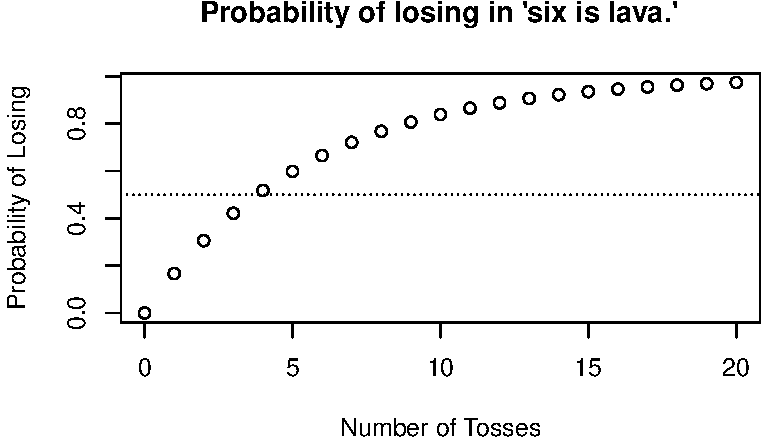
\includegraphics[keepaspectratio]{notes/chapter3_files/figure-pdf/unnamed-chunk-2-1.pdf}}

\end{tcolorbox}

\end{example}

\subsection{Tree Diagrams}\label{tree-diagrams}

Sometimes it is helpful to express counting rules graphically. To do so
we rely on tree diagrams.

\begin{definition}[Tree
Diagram]\protect\hypertarget{def-tree-diagram}{}\label{def-tree-diagram}

A tree diagram is a graphical representation for the product rule for
counting. Specifically, a tree diagram puts each of the decisions in
sequence, and draws a branch for each separate option, starting from the
branches drawn at the previous decision step.

\end{definition}

To draw a tree diagram, you start with the first choice, drawing one
branch for each of the \(n_1\) alternatives, labelling each. Then, at
the second choice, you do the same process at the end of each of the
branches you drew for choice \(1\), this time drawing \(n_2\) branches
there (so you will have just drawn \(n_1\times n_2\) branches). Then for
each of those you draw the \(n_3\) further branches, and so on and so
forth until the end.

If you want to know the total number of choices, you count the end
points at the very end of the diagram. Each branch corresponds to a
single option. To determine which combination of choices it corresponds
to, you read off the branch labels at each branch you take. If you want
to know how many possible combinations come with certain options
selected, you can look at only those branches which are downstream from
the choices that you care about.

\begin{figure}[H]

\caption{\label{fig-tree-diagram-general}A generic tree diagram. Here
the first choice has three different options and the second choice has
two. We can see the six total combinations, labelled on the right of the
diagram, and can trace the choices required to get there.}

\centering{

\pandocbounded{\includegraphics[keepaspectratio]{graphics/ch3-tree-diagram-generic.png}}

}

\end{figure}%

While tree diagrams can be quite useful for visualizing a problem, they
often grow to be overly complex. As a result, we need to fall back on
the numerical representation afforded to us through the product rule for
counting. Counting problems, in general, can very quickly become large
and complex. For this reason, we have several tools to assist us in
reducing this complexity based on common types of problems that we would
like to count.

\subsection{The Factorial}\label{the-factorial}

The first useful tool for simplifying these problems is the
\textbf{factorial}. The factorial of an integer, denoted by \(x!\) is
given by the product of all integers from \(x\) to \(1\).\footnote{Factorials
  are exciting because they always look like they are shouting!} That
is, \[x! = x(x-1)(x-2)\cdots(2)(1).\] If we consider the product rule
for counting then note that if \(n_1=1\), \(n_2=2\), \ldots{} ,
\(n_k = k\), then the total number of options is
\(k\times(k-1)\times\cdots\times 1 = k!\). The most common reason that
this comes up is when we want to order a collection of items.

Suppose that you have \(10\) books that you want to place on a shelf.
You can view this as making \(10\) sequential decisions: what book goes
first, second, third, and so on. There are \(10\) options for the first
book, then \(9\) for the second (any except for the first one), \(8\)
for the third (any except for the first \(2\)). This continues down to
the last book, and so we conclude that there are
\(10\times9\times8\times\cdots\times1 = 10!\) ways of arranging these
books.

\begin{example}[Seating in a (Full) Coffee
Shop]\protect\hypertarget{exm-factorial}{}\label{exm-factorial}

One day Charles and Sadie walk into the coffee shop and find that it is
completely full. There are ten seats and ten people sitting in them.
They are disappointed that they do not have room to sit themselves,
however, they are never ones to pass up an interesting probability
question.

\begin{enumerate}
\def\labelenumi{\alph{enumi}.}
\tightlist
\item
  How many different ways could these ten people have sat in these ten
  seats?
\item
  If there are ten drinks that have been made, and one is to be passed
  out to each seat, how many different ways can these ten people sit in
  these ten seats, with each of these ten drinks?
\item
  Alongside the ten drinks, there are ten snacks to be served up as
  well. How many different ways can these ten people sit in these ten
  seats, with each of these ten drinks, and each of these ten snacks?
\end{enumerate}

\begin{tcolorbox}[enhanced jigsaw, arc=.35mm, rightrule=.15mm, breakable, bottomrule=.15mm, left=2mm, toprule=.15mm, leftrule=.75mm, opacityback=0, colback=white, colframe=quarto-callout-color-frame]

\vspace{-3mm}\textbf{Solution}\vspace{3mm}

\begin{enumerate}
\def\labelenumi{\alph{enumi}.}
\item
  Here, we can think about lining up the ten seats in a row, each number
  \(1\) through \(10\). Then, we want to place one patron into each of
  the seats. This is no different from ordering \(10\) books, and so the
  total is \(10!\) which is \(3,628,800\).
\item
  Note that we still have to make the seat choices from part (a), so
  there are \(10!\) ways of getting the \(10\) people sat in the \(10\)
  chairs. Once there, we can think of handing out the drinks to each of
  the numbered combinations of person-chair. This is no different from
  passing out the people as well, giving \(10!\) ways of doing this. We
  use the product rule to combine these two choices, with
  \(10!\times 10!\) total combinations of people-chair-drink. This is
  \(13,168,189,440,000\).
\item
  Extending the same logic before, there are \(10!\times 10!\) ways of
  getting each person sat in a chair with a drink. Then, there will be
  an additional \(10!\) ways of passing out the snacks to these people.
  Taken together this gives \(10!\times 10!\times 10!\) which is
  \(47,784,725,839,872,000,000\).\footnotemark{}
\end{enumerate}

\end{tcolorbox}

\footnotetext{It is somewhat interesting to note how large these values
get relatively quickly. This is a comparatively small question: only
\(10\) people with \(10\) drinks and \(10\) snacks. If you consider any
counting problem with a larger number of items, these problems quickly
grow to be intensely complex. For instance, a count of my main home book
collection reveals \(376\) of them. To order these would give \(376!\)
possible orderings. In decimal representation this is
\[4.992244775852435618292576458782762114148884082811840265632\dots\times10^{806}.\]
This is an \(807\) digit long number. This is an incomprehensibly large
number. This number is \(8×10^{726}\) \textbf{times larger than} the
number of atoms in the universe. That is, if every atom in the universe
were given some arrangements of books to hold onto, they would need to
hold \(8×10^{726}\) of them in order for all of the arrangements to be
held. I point this out because combinatorics \emph{explodes} in this
way. Even simple problems grow out of hand very, very quickly. This is
where comfort with the algebraic tools is required, rather than a
reliance on intuition. There is simply no way to have intuition
regarding the scope of these numbers, at least, not without a lot of
practice.}

\end{example}

\begin{remark}[0!]
Depending on how factorials are thought of, some trouble can come up
around a quantity like \(0!\). On one hand, if we view factorials as
multiplying each number between \(n\) and \(1\) together then
\(0! = 0\times 1\) and we get \(0! = 0\). On the other hand, if we view
factorials as counting the number of ways which we can order a set of
\(n\) items, then \(0!\) is the number of ways we can order \(0\) items,
which is \(1\).\footnote{Imagine I am placing books on my shelf. With
  \(3\) books there are \(3! = 6\) ways my shelf can look at the end.
  With \(2\) books there are \(2! = 2\) ways my shelf can look at the
  end. With \(1\) book there are \(1! = 1\) ways my shelf can look at
  the end. With \(0\) books there are \(0! = 1\) ways my shelf can look
  at the end.} So, which is it?

We take \(0!\) to be equal to \(1\). The ordering argument is perhaps
the most convincing. However, if you are algebraically minded you may
wonder how we get around the tricky issue of using our algebraic
definition. The key insight is to not define \(n!\) as the product of
the numbers from \(n\) to \(1\), but rather, to define
\[(n-1)! = \frac{n!}{n},\] and specify that \(1! = 1\). Then in this
case we get all of the usual requirements for how we have discussed
factorials, but we also get that \(0! = \dfrac{(0+1)!}{(0+1)} = 1\). As
a result, we will take \(0! = 1\).\footnote{Note, this does not help us
  with the factorials of negative numbers, nor of fractional numbers.
  Factorials \emph{can} be extended to these in sensible ways, but these
  are not for combinatorial purposes and are no longer ``factorials''
  exactly.}
\end{remark}

\subsection{Permutations and
Combinations}\label{permutations-and-combinations}

Sometimes, we want to order items from a collection, but we want to only
take a subset of these items. That is, suppose that you have \(20\)
books, only \(9\) of them will fit on the shelf, and you want to know
``how many ways can you put \(9\) books on the shelf, in order, from
your collection of \(20\)?'' Using the product rule of counting for this
directly, we recognize that there are \(20\) options for the first, then
\(19\), then \(18\), and so on until there are \(12\) choices for the
\(9\)th book to place. We can write this out in a seemingly strange way.
\begin{align*}
  &\ (20)(19)(18)(17)(16)(15)(14)(13)(12) \\ 
  &= \frac{(20)(19)(18)(17)(16)(15)(14)(13)(12)(11)(10)(9)(8)(7)(6)(5)(4)(3)(2)(1)}{(11)(10)(9)(8)(7)(6)(5)(4)(3)(2)(1)} \\
  &= \frac{(20)(19)(18)(17)(16)(15)(14)(13)(12)\cancel{(11)}\cancel{(10)}\cancel{(9)}\cancel{(8)}\cancel{(7)}\cancel{(6)}\cancel{(5)}\cancel{(4)}\cancel{(3)}\cancel{(2)}\cancel{(1)}}{\cancel{(11)}\cancel{(10)}\cancel{(9)}\cancel{(8)}\cancel{(7)}\cancel{(6)}\cancel{(5)}\cancel{(4)}\cancel{(3)}\cancel{(2)}\cancel{(1)}}
\end{align*}

This expression is \(20!\) divided by \(11!\), and gives the same as our
argument from the product rule for counting directly. This is a more
general result than our example with books would suggest. If we have
\(n\) items, and we want to choose \(k\) of them taking into account the
order those choices, it will always be \(n!\) divided by \((n-k)!\). We
call this a permutation.

\begin{definition}[Permutations]\protect\hypertarget{def-permutation}{}\label{def-permutation}

If we wish to select \(k\) items from a collection of \(n\) items, where
the ordering of these selections matters, then the total number is
referred to as a permutation. Mathematically,
\[P_{n,k} = \frac{n!}{(n-k)!}.\]

\end{definition}

Permutations arise when we select ordered subsets from a collection. We
often, in combinatorial problems, talk about ordering, though sometimes
what we mean by this is slightly more abstract. Suppose that you want to
form a committee with \(5\) different people, each of which occupies a
different role: the president, vice president, treasurer, note taker,
and critic. If there are \(30\) people to select for this then there are
\(P_{30,5}\) total possible committees that can be formed. While there
is not a sequential order here, we talk about this as being ``ordered''
since we can differentiate between the five roles. Instead of labelling
them with their names, we could label them \(1\) through \(5\) and make
the ordering more explicit.

\begin{example}[Seating in a (Not Full) Coffee
Shop]\protect\hypertarget{exm-permutations}{}\label{exm-permutations}

Still haunted by that time when the coffee shop was full, Sadie and
Charles enter the coffee shop at a later date and find that, including
themselves, there are only \(7\) patrons in the store, and still the
\(10\) seats to choose from.

\begin{enumerate}
\def\labelenumi{\alph{enumi}.}
\tightlist
\item
  How many different ways can the \(7\) people sit in the \(10\)
  different chairs?
\item
  If there are \(10\) drinks on the menu, how many different ways can
  each person choose a chair and a drink?
\item
  If the coffee shop can make only one of each drink, how does the
  previous total change?
\end{enumerate}

\begin{tcolorbox}[enhanced jigsaw, arc=.35mm, rightrule=.15mm, breakable, bottomrule=.15mm, left=2mm, toprule=.15mm, leftrule=.75mm, opacityback=0, colback=white, colframe=quarto-callout-color-frame]

\vspace{-3mm}\textbf{Solution}\vspace{3mm}

\begin{enumerate}
\def\labelenumi{\alph{enumi}.}
\item
  In this case we are looking to order subsets from a total collection.
  If we line up the \(7\) patrons we then need to select \(7\) chairs to
  go with them, and keep these ordered. This is
  \[P_{10,7} = \frac{10!}{3!} = 604800.\]
\item
  In this part of the question we know that the \(7\) people have
  \(P_{10,7}\) ways of sitting into seats, we can view this as decision
  one. Then, for each of these \(7\) people there is a decision of what
  drink they will order. For these \(7\) decisions,
  \(n_2 = \cdots = n_8 = 10\). As a result, we get the total number is
  \[P_{10,7}\times10\times10\times\cdots\times10 = P_{10,7}\times 10^{7} = 6,048,000,000,000.\]
\item
  This setting, like part (b) starts with a first decision involving
  \(P_{10,7}\) choices. Then, instead of there being \(7\) more
  decisions with \(10\) choices each, we can either view this as \(7\)
  more choices with a descending number of options \(10\) for the first,
  then \(9\), and so on, or we can view this as a single choice where we
  need to select \(7\) \textbf{ordered} options from the \(10\) drinks
  available. This gives \[P_{10,7} \times P_{10,7} = 365,783,040,000,\]
  total choices.
\end{enumerate}

\end{tcolorbox}

\end{example}

Factorials compute the number of orderings for a set of objects, and
permutations compute the number of ordered subsets from a collection of
objects. What about when we do not wish to differentiate the order of
subsets? Suppose that you still need to form a \(5\) person committee,
but you do not have explicit roles for the different members of the
committee. Here we cannot use a permutation directly, as we know that
this takes into account the order.

To determine the number of unordered subsets, we will consider an
alternative approach that we could have used for taking ordered subsets.
Suppose that we formulate the ordered committee as a two step procedure.
First, we select \(5\) people without concern for their order. Then we
choose which order they will have. If \(M\) represents the number of
unordered sets of \(5\) from this population, the product rule for
counting tells us that the total number of ordered committees will be
\(M\times 5!\), since there are \(5!\) arrangements of the \(5\) people.
Thus, we can write this down as
\[P_{30,5} = \frac{30!}{25!} = M\times 5! \implies M = \frac{30!}{25!5!}.\]

This will be true in general. If we want to select \(k\) items from a
collection of \(n\), we will have \(n!\) divided by the product of
\(k!\) and \((n-k)!\). We refer to these as combinations.

\begin{definition}[Combinations]\protect\hypertarget{def-combinations}{}\label{def-combinations}

If we wish to select \(k\) items from a collection of \(n\) items, where
the ordering of these selections does not matter, then the total number
is referred to as a combination. Mathematically,
\[\binom{n}{k} = \frac{n!}{k!(n-k)!}.\]

\end{definition}

We read \(\dbinom{n}{k}\) as ``\(n\) choose \(k\)'', which translates to
``select \(k\) items from a population of \(n\) total options, without
concern for their order.''

To summarize: factorials allow us to order a complete collection,
permutations allow us to select a subset with consideration of the
ordering, and combinations allow us to select a subset from the
collection without regard to the order. These three techniques can be
used in combination with the product rule for counting to allow us to
have very complex total summations.

\begin{example}[Changing the Seating in the Coffee
Shop]\protect\hypertarget{exm-combinations}{}\label{exm-combinations}

Some nights, the coffee shop hosts local music acts. Because of the
added equipment, the coffee shop owners only keep out the number of
seats that are going to be required based on the number of tickets that
were sold.

\begin{enumerate}
\def\labelenumi{\alph{enumi}.}
\tightlist
\item
  If there are \(8\) tickets sold, how many different combinations of
  the \(10\) chairs can get left out?
\item
  Suppose that only \(6\) people end up showing up. How many different
  ways can the \(6\) people sit in the \(8\) chairs that are being
  selected from the \(10\) total possibilities?
\end{enumerate}

\begin{tcolorbox}[enhanced jigsaw, arc=.35mm, rightrule=.15mm, breakable, bottomrule=.15mm, left=2mm, toprule=.15mm, leftrule=.75mm, opacityback=0, colback=white, colframe=quarto-callout-color-frame]

\vspace{-3mm}\textbf{Solution}\vspace{3mm}

\begin{enumerate}
\def\labelenumi{\alph{enumi}.}
\item
  Here, there is no ordering for the \(8\) chairs that are to be
  selected. As a result, we are looking for how many chairs can be
  selected from a group of \(10\) of them. This is
  \[\binom{10}{8} = \frac{10!}{8!\cdot 2!} = 45.\]
\item
  With the first choice having \(45\) possible options, the second
  choice that needs to be made is how \(6\) people sit into \(8\)
  chairs. Here the ordering \emph{does} matter, since the chairs are
  distinguishable. As a result, this is a permutations question, with
  there being a total of \(P_{8,6} = \frac{8!}{2!}\) ways of having the
  people select their seats. In total then there are
  \[\binom{10}{8}\times P_{8,6} = \frac{10!}{8!\cdot 2!}\cdot\frac{8!}{2!} = 907,200.\]
\end{enumerate}

\end{tcolorbox}

\end{example}

\begin{example}[Fundraiser Raffle
Consultation]\protect\hypertarget{exm-combinations-and-permutations}{}\label{exm-combinations-and-permutations}

Charles and Sadie are asked by a local organization to help organize a
raffle as a fundraiser. The organizers are considering two different
versions for the raffle.

\begin{enumerate}
\def\labelenumi{\arabic{enumi}.}
\tightlist
\item
  They would sell \(1000\) tickets, and there are \(5\) different prizes
  (valued at \$1000, \$500, \$250, \$150, and \$100) respectively.
\item
  They would sell \(1000\) tickets, and draw \(5\) winners. Each winner
  would win \$400.
\end{enumerate}

They are curious how these two scenarios differ statistically.

\begin{enumerate}
\def\labelenumi{\alph{enumi}.}
\tightlist
\item
  How many possible winning combinations exist for scenario 1?
\item
  How many possible winning combinations exist for scenario 2?
\item
  Are the probabilities that any specific individual wins the raffle
  different between the two versions? Explain.
\end{enumerate}

\begin{tcolorbox}[enhanced jigsaw, arc=.35mm, rightrule=.15mm, breakable, bottomrule=.15mm, left=2mm, toprule=.15mm, leftrule=.75mm, opacityback=0, colback=white, colframe=quarto-callout-color-frame]

\vspace{-3mm}\textbf{Solution}\vspace{3mm}

\begin{enumerate}
\def\labelenumi{\alph{enumi}.}
\item
  In the first scenario, the ordering of the winners matters. We can
  think of drawing the \(5\) winners in order from highest value prize
  to lowest value prize. Then, we are selecting \(k=5\) from \(n=1000\)
  with concern for ordering, so the total number of winning combinations
  is \[P_{1000,5} = \frac{1000!}{995!} = 990,034,950,024,000.\]
\item
  In the second scenario, the ordering of the winners does not matter.
  There is no distinction between the winners, and so we could select
  any \(5\) and then report the winners alphabetically. Then, we are
  selecting \(k=5\) from \(n=1000\) with no concern for ordering, so the
  total number of winning combinations is
  \[\binom{1000}{5} = \frac{1000!}{5!995!} = 8,250,291,250,200.\]
\item
  Intuitively, the probabilities should be the same. Moreover, it makes
  sense that each probability should be \(5/1000\) since the probability
  of winning any of the prizes is \(1/1000\) and there are \(5\) such
  prizes to win.

  In parts (a) and (b) we saw the total number of each version, and we
  know that any sequence of winners is equally likely. As a result, we
  can consider counting the total number of ways that any specific
  individual can win in both scenarios. In the first, suppose that the
  individual wins the top prize. Then we need to select 4 other winners
  (with ordering) from the remaining \(999\) individuals. Thus, the
  total number of ways that they can win the \$1000 prize is
  \(P_{999,4}\). The same goes for all of the other prizes, meaning the
  total number of ways that they can win is \(5\times P_{999,4}\). Thus,
  the probability that they win is
  \[\frac{5P_{999,4}}{P_{1000,5}} = \frac{5(999!/995!)}{1000!/995!} = \frac{5}{1000}.\]

  For the second option, if we know that the particular individual wins
  then we need to select the other \(4\) winners from the remaining
  \(999\) individuals, without concern for the ordering. Thus, there are
  \(\dbinom{999}{4}\) winning combinations for the specific individual,
  and the probability that they win is
  \[\frac{\binom{999}{4}}{\binom{1000}{5}} = \frac{999! \times 5! \times 995!}{995!\times 4! \times 1000!} = \frac{5}{1000}.\]
\end{enumerate}

\end{tcolorbox}

\end{example}

\subsection{Less Common Counting
Techniques}\label{less-common-counting-techniques}

While most of the problems we address will revolve around permutations
and combinations (with heavy use of the product rule), there are
additional techniques which are important to know (and recognize when to
use). In particular, combinations and permutations each assume that we
are sampling from our set \textbf{without replacement}. That is, each
time you select an item, it is removed from the population. These are
the most common situations in these combinatorial problems, however,
there are \emph{some} situations which arise where we need to count the
number of ordered or unordered subsets \emph{with} replacement.

\subsubsection{Ordered Subsets with
Replacement}\label{ordered-subsets-with-replacement}

Consider, for instance, forming a password using only lowercase numbers
and letters. If you decide on a fixed length for the password, then
there are going to be \(36\) choices at each decision point, and you
want to take an ordered subset of these. This is forming an
\textbf{ordered subset with replacement}, and to count how many
different ways there are of doing this, we can use the product rule.
That is, you have \(36\) choices at each decision point, and so there
are \(36\times 36\times\cdots\times 36 = 36^k\) total decisions, where
\(k\) is the number of items to select.

In general, if you have \(n\) total items and you want to make an
ordered set of \(k\) of these items \textbf{with replacement} you will
have \(n^k\) total ways of doing this.

\subsubsection{Unordered Subsets with
Replacement}\label{unordered-subsets-with-replacement}

Forming unordered sets with replacement is slightly less intuitive.
Consider rolling \(k\) dice which are not distinguishable from one
another. We know that there are \(6\) total sides that can show up on
each of these dice, but how many different combinations of numbers can
show up overall? If the dice can be distinguished we would say that
there are \(6^k\) possible ways of doing this. However, some of these
combinations are going to be equivalent in the unordered world. Take the
simple case of \(k=2\). Here we have the following possibilities:
\begin{align*}
(1, 1), (1, 2), (1, 3), (1, 4), (1, 5), (1, 6)&\\ 
(2, 2), (2, 3), (2, 4), (2, 5), (2, 6)&\\ 
(3, 3), (3, 4), (3, 5), (3, 6)&\\ 
(4, 4), (4, 5), (4, 6)&\\ 
(5, 5), (5, 6)&\\ 
(6,6)&
\end{align*}

This gives a total of \(21\) possible combinations, rather than \(36\).

In general, if we want to find the way of selecting \(k\) elements
\emph{with replacement} from a total of \(n\), then the number of ways
of doing this will be \[\binom{n+k-1}{k}.\] In our example this gives
\(\binom{6+2-1}{2} = 21\).

\subsubsection{Permutations with Identical
Objects}\label{permutations-with-identical-objects}

Finally, it is worth understanding how to handle identical objects in
combinatorial problems. Suppose that, of the \(10\) books that we wish
to place on a shelf, we have \(2\) copies of one of them, \(3\) copies
of another one, and the other \(5\) have one copy each. Supposing that
there is no way to tell these identical objects apart, how many ways can
we arrange the bookshelf?

First, if we pretend that all of the items are actually able to be
differentiated then there are \(10!\) ways of placing these books. Now,
in any of these permutations, had we swapped the order of the first book
(with \(2\) copies) the ordering would have been indistinguishable. As a
result, for every ordering of the \(8\) other books, we counted that
permutation twice (when it should have only been counted once!). So to
address the two repeated copies we need to take \(10!/2\). Now, a
similar argument is going to hold for the book with \(3\) repeated
copies. However, instead of there being \(2\) permutations which are
identical, there are going to be \(3! = 6\) permutations which are
identical. This is because we can reorder the \(3\) copies of the book
in anyway we choose, and still wind up with the same overall
permutation.\footnote{In fact, the reason that there are \(2\) ways of
  doing this with the book with \(2\) copies is since \(2! = 2\).} As a
result, the total number is going to be
\[\frac{10!}{2!\cdot3!} = 302400.\]

We can see this same result through an alternative construction. First,
we select which of the \(10\) slots should have the first book. We do
not care about the order, and so there are \(\binom{10}{2}\) ways of
doing this. Next, we can select which of the \(8\) remaining slots
should have the second book. Like the first one there will be
\(\binom{8}{3}\) ways of placing these. Now, there are \(5\) slots
remaining, and \(5\) books to place, so as a result, we can order those
in \(5!\) different ways, and then slot them into the remaining places
in order. This gives, in total
\[\binom{10}{2}\binom{8}{3}(5!) = \frac{10!}{2!\cancel{8!}}\cdot\frac{\cancel{8!}}{3!\cancel{5!}}\cdot\cancel{5!} = \frac{10!}{2!3!}.\]

To generalize this, if we want to order \(n\) elements, such that there
are \(k\) distinguishable elements with \(n_1\) of the first type,
\(n_2\) of the second, and so forth until \(n_k\) of the last type
(\(n = n_1 + n_2 + \cdots + n_k\)), then the total number of orderings
will be \[\frac{n!}{n_1!\cdot n_2!\cdots n_k!}.\]

\section{From Combinatorics to
Probability}\label{from-combinatorics-to-probability}

While combinatorics is a field of study on its own, with many intriguing
tools and developments surrounding the enumeration of objects, for the
purposes of simple probability models these tools will suffice.
Ultimately, we care about counting since in the equal probability model,
the probability of any event can be determined by counting the number of
ways that the event can occur and dividing by the total number of
outcomes that are possible. That is, we use these tools to derive
\(N_A\), the total number of ways that \(A\) can occur, and \(N\), the
total number of experimental outcomes, and then we conclude that
\[P(A) = \frac{N_A}{N}.\]

\begin{example}[Poker Hand
Counts]\protect\hypertarget{exm-poker-hands}{}\label{exm-poker-hands}

During one of their conversations, Charles and Sadie were remarking how
they never really played poker. As they understand it, in poker you are
dealt a hand of \(5\) cards and you want to use these \(5\) cards to try
to match certain sets of cards, some of which are more rare than others.
Charles and Sadie start to get hung-up on discussions regarding
``straights'' and ``flushes''.

A straight is any sequence of \(5\) cards in ascending order (where aces
can be low, or high). For instance, \(7, 8, 9, 10, \text{J}\) of any
suit. A flush, is any set of \(5\) cards belonging to the same suit.
Charles just \emph{feels} that straights have to be more rare than
flushes.

\begin{enumerate}
\def\labelenumi{\alph{enumi}.}
\tightlist
\item
  How many different straights are there from a standard deck of cards?
\item
  How many different flushes are there from a standard deck of cards?
\item
  If dealt \(5\) cards at random, what is the probability of a flush?
  What is the probability of a straight?
\item
  A straight flush occurs when you have \(5\) cards in order, of the
  same suit. What is the probability of a straight flush?
\item
  If straight flushes were not counted as flushes, and not counted as
  straights, how do the probabilities of either hand change?
\end{enumerate}

\begin{tcolorbox}[enhanced jigsaw, arc=.35mm, rightrule=.15mm, breakable, bottomrule=.15mm, left=2mm, toprule=.15mm, leftrule=.75mm, opacityback=0, colback=white, colframe=quarto-callout-color-frame]

\vspace{-3mm}\textbf{Solution}\vspace{3mm}

\begin{enumerate}
\def\labelenumi{\alph{enumi}.}
\item
  A straight necessitates drawing five cards in order, with each of any
  suit. Just as with the straight flush, there are \(10\) possible
  starting values for the straight. Once we have selected the starting
  value, then for each of the five cards we can pick any of the four
  suits, resulting in \(4\) choices each. That gives
  \[N_A = 10\times 4\times 4\times 4\times 4\times 4 = 10\times 4^5 = 10240.\]
\item
  A flush necessitates drawing \textbf{any} five cards from the same
  suit. If we had a suit fixed, there would be \({13\choose 5}\) ways of
  doing this, since we do not care about ordering. If we think about
  first choosing the suit, we have \(4\) ways of doing that, resulting
  in \[N_A = 4 \times {13 \choose 5} = 5148.\]
\item
  To find the probabilities of each of these, we need to know the total
  number of \(5\) card hands. We do not consider order, and so
  \(N = \binom{52}{5} = 2598960\). Then, the probability is the number
  of combinations (calculated above) divided by the number of hands.
  This gives, for straights,
  \[P(A) = \frac{10240}{2598960} = \frac{128}{32487} \approx 0.00394,\]
  and for flushes,
  \[P(A) = \frac{5148}{2598960} = \frac{33}{16660} \approx 0.00198.\] As
  a result, we see that straights are roughly twice as common as flushes
  are.\footnotemark{}
\item
  Note that to form a straight flush, we first have to fix a suit. There
  are \({4\choose 1}=4\) total ways of doing this. Next, we need to pick
  which starting value we will use. Once a card has been selected as a
  starting value, the remaining cards are fixed. The start value ranges
  from A through to \(10\). Correspondingly, we have
  \[N_A = {4\choose 1}{10 \choose 1} = 4\times10 = 40.\] As a result, we
  get that \[P(A) = \frac{40}{2598960} = \frac{1}{64974}.\]
\item
  From (d) exactly \(40\) of the straights and \(40\) of the flushes are
  also straight flushes. We can thus remove \(40\) from the totals of
  each of these, giving \(\dfrac{10200}{2598960}\) for straights and
  \(\dfrac{5108}{2598960}\) for flushes.
\end{enumerate}

\end{tcolorbox}

\footnotetext{This is \emph{still} a deeply unintuitive result to me. To
me it feels like it should be harder to get a nice ordering of cards all
in a row than it is to find ones of the same suit. And yet, it is about
twice as likely to have the straights. Now, if you think about this
deeply, it makes a lot of sense: there is a lot more leeway in selecting
the straight than the flush. However, my brain refuses to accept this as
intuitive. This is something that can often occur in probability
questions where the true results can be far from what we would expect.
An interesting question is how long does a straight have to be to be
less likely than a flush of the same length. Note that the number of
ways of choosing a flush will always be \(4\times\binom{13}{k}\), and
the number of ways of forming a straight will always be
\(10\times 4^k\). If we consider \(k\) from \(1\) to \(13\), we can take
the ratios of these to see just how much more (or less) likely a
straight is. Doing this gives: {k=1 gives 0.769. k=2 gives 0.513. k=3
gives 0.559. k=4 gives 0.895. k=5 gives 1.989. k=6 gives 5.967. k=7
gives 23.869. k=8 gives 127.304. k=9 gives 916.587. k=10 gives 9165.874.
k=11 gives 134432.821. k=12 gives 3226387.692. k=13 gives 167772160.} Up
to (and including) \(4\) cards the straight is indeed harder to achieve.
However, this does not last long!}

\end{example}

\section*{Exercises}\label{exercises-1}
\addcontentsline{toc}{section}{Exercises}

\markright{Exercises}

\begin{exercise}[]\protect\hypertarget{exr-3.1}{}\label{exr-3.1}

The probability that a smartphone breaks during the first year of use is
\(0.19\). What is the probability that it does not break during the
first year?

\end{exercise}

\begin{exercise}[]\protect\hypertarget{exr-3.2}{}\label{exr-3.2}

Assuming that \(A\) and \(B\) are disjoint, which of the following
statements are always true.

\begin{enumerate}
\def\labelenumi{\alph{enumi}.}
\tightlist
\item
  \(P(A\cup B) = 0\).
\item
  \(P(A \cap B) = 0\).
\item
  \(P(A \cup B) = P(A \cap B)\).
\item
  \(P(A \cup B) = P(A) + P(B)\).
\end{enumerate}

\end{exercise}

\begin{exercise}[]\protect\hypertarget{exr-3.3}{}\label{exr-3.3}

A ball is drawn at random from a box containing \(6\) red balls, \(4\)
white balls, and \(5\) blue balls. Determine the probabilities
associated with the following events.

\begin{enumerate}
\def\labelenumi{\alph{enumi}.}
\tightlist
\item
  The ball is red.
\item
  The ball is white.
\item
  The ball is blue.
\item
  The ball is not red.
\item
  The ball is red or white.
\end{enumerate}

\end{exercise}

\begin{exercise}[]\protect\hypertarget{exr-3.4}{}\label{exr-3.4}

A survey of high schoolers were asked about where they most prefer to
spend their time when they are at home. The results were:

\begin{itemize}
\tightlist
\item
  Bedroom: \(0.37\);
\item
  Living Room: \(0.26\);
\item
  Den: \(0.22\);
\item
  Basement: \(0.12\);
\item
  Kitchen: \(0.02\);
\item
  Bathroom: \(0.01\).
\end{itemize}

\begin{enumerate}
\def\labelenumi{\alph{enumi}.}
\tightlist
\item
  What is the probability that a student prefers being in their living
  room or den?
\item
  What is the probability that a student does not prefer being in their
  bedroom?
\end{enumerate}

\end{exercise}

\begin{exercise}[]\protect\hypertarget{exr-3.5}{}\label{exr-3.5}

Let \(S\) be the event that a randomly selected college student has
taken any statistics course, and \(C\) be the event that a randomly
selected college student has taken any chemistry course. Suppose
\(P(S) = 0.5\), \(P(C) = 0.15\), and \(P(S\cap C) = 0.12\).

\begin{enumerate}
\def\labelenumi{\alph{enumi}.}
\tightlist
\item
  Find the probability that the student has taken either a statistics or
  chemistry course.
\item
  Find the probability that a student has taken neither chemistry nor
  statistics.
\item
  Find the probability that a student has taken statistics but not
  chemistry.
\end{enumerate}

\end{exercise}

\begin{exercise}[]\protect\hypertarget{exr-3.6}{}\label{exr-3.6}

Let \(M\) be the event that a student passes their math exam, and let
\(H\) be the event that a student passes their history exam. Suppose
that \(P(M) = 0.85\), \(P(H) = 0.95\), and \(P(M\cup H) = 0.99\).

\begin{enumerate}
\def\labelenumi{\alph{enumi}.}
\tightlist
\item
  Find the probability that the student passes both math and history.
\item
  Find the probability that the student passes neither math, nor
  history.
\item
  Find the probability that the student passes math, but not history.
\end{enumerate}

\end{exercise}

\begin{exercise}[]\protect\hypertarget{exr-3.7}{}\label{exr-3.7}

A medical clinic screening for a particular disease classifies its
patients into three health risk categories: low risk, moderate risk, and
high risk. Suppose that \(70\%\) of the patients are categorized low
risk, \(20\%\) are categorized as moderate risk, and \(10\%\) are
categorized as high risk. Suppose a patient is randomly selected.

\begin{enumerate}
\def\labelenumi{\alph{enumi}.}
\tightlist
\item
  What is the probability that the patient is categorized as low risk?
\item
  What is the probability that the patient is not categorized high risk?
\end{enumerate}

\end{exercise}

\begin{exercise}[]\protect\hypertarget{exr-3.8}{}\label{exr-3.8}

Two different designs are being considered for a particular mechanical
system. For each, determine the probability that the system continues to
function.

\begin{enumerate}
\def\labelenumi{\alph{enumi}.}
\tightlist
\item
  The system contains two components, \(A\) and \(B\). The system will
  continue to function so long as either \(A\) or \(B\) functions. The
  probability that \(A\) functions is \(0.95\), the probability that
  \(B\) functions is \(0.90\), and the probability that the both
  function is \(0.88\).
\item
  The system contains two components, \(A\) and \(B\). The system will
  continue to function only if both \(A\) and \(B\) function. The
  probability that \(A\) functions is \(0.98\), the probability that
  \(B\) functions is \(0.95\), and the probability that at least one is
  functioning is \(0.99\).
\end{enumerate}

\end{exercise}

\begin{exercise}[]\protect\hypertarget{exr-3.9}{}\label{exr-3.9}

A hotel chain is concerned about the cleanliness of their rooms, so they
send two inspectors to check on this. Inspector A visually inspects
\(1000\) rooms and found \(37\) of them to be inadequately cleaned.
Inspector B visually inspects the same rooms found \(43\) of them to be
lacking sufficient cleanliness. A total of \(948\) rooms were found to
be clean by both inspectors.

\begin{enumerate}
\def\labelenumi{\alph{enumi}.}
\tightlist
\item
  Find the probability that a randomly selected room has an issue that
  was found by at least one of the two inspectors.
\item
  Find the probability that a randomly selected room has an issue that
  was found by both inspectors.
\item
  Find the probability that a randomly selected room has an issue that
  was found by inspector \(A\) but not by inspector \(B\).
\end{enumerate}

\end{exercise}

\begin{exercise}[]\protect\hypertarget{exr-3.10}{}\label{exr-3.10}

Let \(A\) and \(B\) be events with probabilities \(P(A) = \dfrac{3}{4}\)
and \(P(B) = \dfrac{1}{3}\). Show that
\[\frac{1}{12}\leq P(A\cap B)\leq\frac{1}{3}.\]

\end{exercise}

\begin{exercise}[]\protect\hypertarget{exr-3.11}{}\label{exr-3.11}

Find the probability of a \(4\) turning up at least once in two tosses
of a fair die.

\end{exercise}

\begin{exercise}[]\protect\hypertarget{exr-3.12}{}\label{exr-3.12}

It is required to place \(5\) hardcovers and \(4\) paperbacks onto a
bookshelf, so that each of the paperbacks are between two hardcovers.
How many ways can this be done?

\end{exercise}

\begin{exercise}[]\protect\hypertarget{exr-3.13}{}\label{exr-3.13}

A committee of eight people must choose a president, a vice-president,
and a secretary. In how many ways can this be done?

\end{exercise}

\begin{exercise}[]\protect\hypertarget{exr-3.14}{}\label{exr-3.14}

~

\begin{enumerate}
\def\labelenumi{\alph{enumi}.}
\tightlist
\item
  One drawer in a dresser contains \(8\) blue socks and \(6\) white
  socks. Another drawer contains \(4\) blue socks and \(2\) white socks.
  One sock is chosen from each drawer. What is the probability that they
  match?
\item
  A third drawer contains \(6\) red socks, \(4\) green socks, and \(2\)
  black socks. Two socks are selected at random. What is the probability
  that they match.
\end{enumerate}

\end{exercise}

\begin{exercise}[]\protect\hypertarget{exr-3.15}{}\label{exr-3.15}

A company has hired \(15\) new employees, and must assign \(6\) to the
day shift, \(5\) to the graveyard shift, and \(4\) to the night shift.
In how many different ways can the shifts be made?

\end{exercise}

\begin{exercise}[]\protect\hypertarget{exr-3.16}{}\label{exr-3.16}

A group of \(10\) people have gotten together to play basketball. They
will begin by dividing themselves into two teams of \(5\) players each.
One team will wear red and the other blue. How many ways can this be
done?

\end{exercise}

\begin{exercise}[]\protect\hypertarget{exr-3.17}{}\label{exr-3.17}

A factory produces a total of \(15,000\) candies a day, of which \(3\%\)
do not pass quality standards. Find the probability that, out of \(500\)
candies chosen at random on a single day, \(12\) are deemed insufficient
quality.

\end{exercise}

\begin{exercise}[]\protect\hypertarget{exr-3.18}{}\label{exr-3.18}

A shelf has \(6\) mathematics books and \(4\) physics books. If these
were randomly ordered, what is the probability that \(3\) particular
mathematics books will be together.

\end{exercise}

\begin{exercise}[]\protect\hypertarget{exr-3.19}{}\label{exr-3.19}

Suppose that car license plates consist of three letters followed by
three numbers.

\begin{enumerate}
\def\labelenumi{\alph{enumi}.}
\tightlist
\item
  How many different license plates can be made?
\item
  How many different license plates can be made in which no letter or
  number appears more than once?
\item
  A license plate is chosen at random. What is the probability that no
  letter or number appears more than once?
\end{enumerate}

\end{exercise}

\begin{exercise}[]\protect\hypertarget{exr-3.20}{}\label{exr-3.20}

A game has individuals forming random ``words'' (strings of letters,
whether they have a meaning or not). On a particular turn, one player
must form a word which has \(3\) different vowels, and \(4\) different
consonants, where there are \(7\) total consonants and \(5\) total
vowels to choose from. How many possibilities are there for a valid
word?

\end{exercise}

\begin{exercise}[]\protect\hypertarget{exr-3.21}{}\label{exr-3.21}

Six pairs of socks come in sets: there are two pairs of red socks, two
pairs of white socks, and two pairs with stripes on them. If the socks
are placed randomly into pairs, find the probability that no sock ends
up in a pair with the same pattern.

\end{exercise}

\subsection*{References}\label{references-2}
\addcontentsline{toc}{subsection}{References}

\chapter{Probabilities with More than One
Event}\label{probabilities-with-more-than-one-event}

\section{Marginal and Joint
Probabilities}\label{marginal-and-joint-probabilities}

Up until this point we have primarily focused on assigning probabilities
to particular events. If we have some event of interest, \(A\), then
\(P(A)\) is the probability that \(A\) occurs in any manner. If we are
using our equally likely probability model, then
\(P(A) = \dfrac{N_A}{N}\). This is the probability of the event \(A\)
where nothing else is known at all. If we smooth over anything which
could alter the likelihood, if we have no additional information, if we
want the best guess for the likelihood of occurrence in a vacuum, this
is the probability of interest. We refer to such quantities as marginal
probabilities.

\begin{definition}[Marginal
Probability]\protect\hypertarget{def-marginal-probability}{}\label{def-marginal-probability}

The marginal probability of a single event, \(A\), is the probability
that the event happens without considering any additional information.
This is the probability that the event happens, denoted \(P(A)\).

\end{definition}

It is useful to specifically call these marginal probabilities to
differentiate them from probabilities which depend on two or more
events. Specifically, we can think about taking the intersection of two
events, say \(A \cap B\). In words this is the event that \(A\) occurs
\textbf{and} \(B\) occurs. Until this point we have thought about
solving for probabilities related to intersections as a two-step
procedure: first, find an event \(C = A \cap B\), and then second solve
for the marginal probability of \(C\). While this is a useful technique
for calculation, sometimes it is more useful to think of the probability
of the intersection as the probability of \(A\) and \(B\) occurring
simultaneously. We call this the joint probability of \(A\) and \(B\).

\begin{definition}[Joint
Probability]\protect\hypertarget{def-joint-probability}{}\label{def-joint-probability}

The joint probability of two events, \(A\) and \(B\), is given by the
probability of their intersection. That is, \(P(A\cap B)\). This is
sometimes denoted \(P(A,B)\) and corresponds to the probability that
both \(A\) and \(B\) occur.

The joint probability of more than two events extends in the same way.
Suppose there exists a sequence of events, \(A_1, \dots, A_n\), then the
joint probability of these events is
\[P(A_1,A_2,\dots,A_n) = P\left(\bigcap_{i=1}^n A_i\right).\]

\end{definition}

\section{What are Conditional
Probabilities?}\label{what-are-conditional-probabilities}

Marginal probabilities are often of interest, and frequently are the
best tool for summarizing the overall state of the world, or our
knowledge regarding the state of the world. Joint probabilities can be
useful when working with compound events, or thinking of complex
outcomes. However, there are many scenarios which are not covered by
either the joint or marginal probabilities. In practice we know that
sometimes information that we have will change our understanding of the
probability of an event.

Suppose the event \(A\) corresponds to the event that it snows tomorrow,
in some particular city. It is possible to think about how often it
snows on average, and report a value related to that as \(P(A)\). Now,
what if we know that it is currently the middle of summer, and the city
is in the Norther Hemisphere? In this case, while \(P(A)\) does not
shrink to \(0\), it becomes far less likely than if we did not have that
information. Similarly, if we know that it is winter in the same city,
the likelihood that it snows tomorrow increases. In order to formally
capture this we can introduce the idea of conditional probability.

\begin{definition}[Conditional
Probability]\protect\hypertarget{def-conditional-probability}{}\label{def-conditional-probability}

The conditional probability of an event \(A\) given an event \(B\), is
the probability that \(A\) occurs assuming that we know that \(B\)
occurs. The conditional probability takes into account additional
information codified through the occurrence of an additional event. We
write this quantity as \(P(A|B)\), and will read this as ``the
probability of \(A\) given \(B\).''

\end{definition}

Unlike in the case of marginal probabilities, conditional probabilities
allow us to \emph{condition} on extra pieces of information. Instead of
asking ``what is the probability of this event'', we instead ask,
``given that we know this piece of information, what is the probability
of this event?'' Joint probabilities ask ``what is the probability that
both of these events occur simultaneously'' which is distinct in that we
do not have any additional information about the state of the world when
working with joint probabilities. The subtle distinction becomes quite
powerful, both in terms of manipulating and working with probabilities,
but also in terms of expressing the correct events of interest for
ourselves.

To make use of conditional probabilities, we will think of the process
of \emph{conditioning} on one or more events. We will talk of the
probability of \(A\) conditional on \(B\), where \(A\) and \(B\) are two
events of interest. Intuitively, this it the probability of \(A\)
happening, supposing that we know that \(B\) has already happened.

\begin{example}[Six from the
Sum]\protect\hypertarget{exm-basic-conditional-probability}{}\label{exm-basic-conditional-probability}

Charles and Sadie are playing a new game using two dice. In the game
they each take turns rolling the two dice into a container that the
other player cannot see. They add up the dice and then report this sum
to the other player. The other player then has to guess whether or not
there is a six showing.

\begin{enumerate}
\def\labelenumi{\alph{enumi}.}
\tightlist
\item
  On one round, Charles does not hear the sum that Sadie reports as he
  was not paying attention. Sadie is strict and insists that she will
  not repeat herself. What should Charles guess?
\item
  Determine a strategy which optimizes the likelihood that the guessing
  player will be correct.
\end{enumerate}

\begin{tcolorbox}[enhanced jigsaw, arc=.35mm, rightrule=.15mm, breakable, bottomrule=.15mm, left=2mm, toprule=.15mm, leftrule=.75mm, opacityback=0, colback=white, colframe=quarto-callout-color-frame]

\vspace{-3mm}\textbf{Solution}\vspace{3mm}

\begin{enumerate}
\def\labelenumi{\alph{enumi}.}
\item
  In this case we want the \textbf{marginal probability} of a six
  showing up on the roll of two dice. Take \(E\) to represent the event
  wherein at least one six is showing on the roll of two dice. Thus,
  \(E^C\) is the event that no sixes are showing. There are
  \(5\times 5=25\) (using the product rule for counting) ways of
  \emph{not} rolling a \(6\), meaning that
  \[P(E^C) = \dfrac{25}{36} \implies P(E) = 1 - \dfrac{25}{36} = \dfrac{11}{36}.\]
  Thus, Charles should guess that there is no \(6\) as the probability
  is only \(11/36 \approx 0.31\).
\item
  Here we wish to determine conditional probabilities. We take \(E\) to
  be the event that at least one \(6\) is showing, and then \(S\) to be
  a variable representing the sum of the two dice. For
  \(s= 1, \dots, 12\) we wish to find \(P(E|\{S=s\})\). Notice that for
  \(s=2,\dots,6\) \(P(E|S=s) = 0\). If the sum is \(2\) we know that
  there could not have been a \(6\). Moreover, for \(s=11,12\) we know
  that \(P(E|S=s) = 1\) since the only way to form \(11\) is a five and
  a six, and the only way to form \(12\) is to have two sixes. This
  leaves \(s = 7,\dots,10\) to check. The following table gives the set
  of values, the possible combinations to reach the value, and then the
  combinations that end up involving a \(6\).

  \begin{longtable}[]{@{}lll@{}}
  \toprule\noalign{}
  Value & Combinations & Involving 6 \\
  \midrule\noalign{}
  \endhead
  \bottomrule\noalign{}
  \endlastfoot
  7 & (1,6) (2,5) (3, 4) (4, 3) (5, 2) (6, 1) & (1, 6) (6, 1) \\
  8 & (2,6) (3,5) (4, 4) (5, 3) (6, 2) & (2, 6) (6, 2) \\
  9 & (3,6) (4,5) (5, 4) (6, 3) & (2, 6) (6, 2) \\
  10 & (4, 6) (5, 5) (6, 4) & (4, 6) (6, 4) \\
  \end{longtable}

  Referencing from this table we can read off the following
  probabilities \begin{align*}
  P(E|S=7) &= \dfrac{2}{6} = \dfrac{1}{3}\\
  P(E|S=8) &= \dfrac{2}{5} \\
  P(E|S=9) &= \dfrac{2}{4} \\
  P(E|S=10) &= \dfrac{2}{3}.
  \end{align*} As a result, the best strategy is to guess ``yes'' when a
  \(10\), \(11\), or \(12\) is rolled and to be indifferent to the guess
  when a \(9\) is rolled. Otherwise, guess ``no.''
\end{enumerate}

\end{tcolorbox}

\end{example}

Recall that \(A\) and \(B\), as events, are merely subsets of the sample
space, \(\mathcal{S}\). Each item in either \(A\) or \(B\) is one of the
possible outcomes from the experiment or process that we are observing.
Suppose that we know that \(B\) has occurred. What this means is that,
one of the outcomes in the set \(B\) was the observed outcome from the
experiment. Now, if we want to know \(P(A|B)\), we want to know the
probability, working from the assumption that \(B\) has happened, that
\(A\) also happens. That is, knowing that \(B\) has happened, what is
the probability that \(A\) and \(B\) both happen.

The event that \(A\) and \(B\) both happen is denoted by the
intersection, \(A \cap B\). This corresponds to the set of events inside
the set \(B\) which also belong to the set \(A\). Now, instead of
considering the joint probability directly, we need to acknowledge that
for \(A|B\), only the events in \(B\) were possible. That is, instead of
being divided by the whole space, we can only divide by the space of
\(B\). In some sense, we can view conditioning on \(B\) as treating
\(B\) as though it is the full sample space, and finding probabilities
within that. In general, \(B\) will be smaller than \(\mathcal{S}\), and
so \(P(B) < 1\). Instead of the conditional probability being ``out of''
\(1\), it will instead be ``out of'' \(P(B)\), which gives
\(P(A|B) = \dfrac{P(A\cap B)}{P(B)}\).

\begin{tcolorbox}[enhanced jigsaw, arc=.35mm, title={Computing Conditional Probabilities}, rightrule=.15mm, coltitle=black, opacitybacktitle=0.6, colbacktitle=quarto-callout-tip-color!10!white, leftrule=.75mm, colback=white, breakable, titlerule=0mm, toptitle=1mm, bottomtitle=1mm, bottomrule=.15mm, toprule=.15mm, opacityback=0, left=2mm, colframe=quarto-callout-tip-color-frame]

For an event \(A\), and an event \(B\) with probability \(P(B) > 0\),
the conditional probability of \(A\) given \(B\) is
\[P(A|B) = \dfrac{P(A\cap B)}{P(B)}.\]

\end{tcolorbox}

To make this more clear, suppose that we take \(A\) to be the event that
a \(2\) is rolled on a fair, six-sided die, and \(B\) to be the event
that an even number was rolled. This is an equal probability model, and
so each outcome gets \(\dfrac{1}{6}\) probability. The original sample
space is \(\mathcal{S} = \{1,2,3,4,5,6\}\), the event \(A\) is
\(\{2\}\), and the event \(B\) is \(\{2,4,6\}\). In order for both \(A\)
and \(B\) to occur, we note that we need \(A \cap B = \{2\}\). If we
know that \(B\) has occurred, then we know that either a \(2\), \(4\),
or \(6\) has been rolled, with equal probability for each. Thus,
intuitively, we can view \(B\) as the new sample space, and say that
rolling a \(2\) has a \(\dfrac{1}{3}\) probability, given that there are
\(3\) outcomes and \(1\) of them is the event of interest.

We can also compute this directly. Note that \(P(B) = \dfrac{1}{2}\),
and so we need to scale each event by \(\dfrac{1}{1/2}\) in order to
make sure that the total probability of our reduced sample space equals
\(1\). Then \(P(A\cap B) = \dfrac{1}{6}\), so
\[P(A|B) = \dfrac{1/6}{1/2} = \dfrac{1}{3}.\]

Suppose that, instead of a fair die, it was weighted so that \(6\) comes
up more frequently than the other options. Consider the probability of
observing a six to be \(0.5\), with the other five values each coming up
with probability \(0.10\). If \(A\) and \(B\) are the same events as
above, then \(P(B) = 0.7\).

If we know that \(B\) has occurred then the new sample space is
\(\{2,4,6\}\) where \(P(2) = \dfrac{0.1}{0.7} = \dfrac{1}{7}\),
\(P(4) = \dfrac{0.1}{0.7} = \dfrac{1}{7}\), and
\(P(6) = \dfrac{0.5}{0.7} = \dfrac{5}{7}\). Note that these three
probabilities sum to \(1\) still, which constitutes a valid probability
model, and so \(P(A|B) = \dfrac{1}{7}\).

\begin{example}[Six from the Sum -
Revisited]\protect\hypertarget{exm-basic-conditional-probability-rev}{}\label{exm-basic-conditional-probability-rev}

Sadie sees the solution worked out for the best strategy in the dice
game above, but is having trouble understanding it in the context of
conditional probability more broadly. For the sums \(7, 8, 9\), and
\(10\), describe the process of limiting the sample space to get the
correct conditional probability, and use the formula to show that the
probabilities worked out in
Example~\ref{exm-basic-conditional-probability} are correct.

\begin{tcolorbox}[enhanced jigsaw, arc=.35mm, rightrule=.15mm, breakable, bottomrule=.15mm, left=2mm, toprule=.15mm, leftrule=.75mm, opacityback=0, colback=white, colframe=quarto-callout-color-frame]

\vspace{-3mm}\textbf{Solution}\vspace{3mm}

The relevant table of solutions is copied from above.

\begin{longtable}[]{@{}lll@{}}
\toprule\noalign{}
Value & Combinations & Involving 6 \\
\midrule\noalign{}
\endhead
\bottomrule\noalign{}
\endlastfoot
7 & (1,6) (2,5) (3, 4) (4, 3) (5, 2) (6, 1) & (1, 6) (6, 1) \\
8 & (2,6) (3,5) (4, 4) (5, 3) (6, 2) & (2, 6) (6, 2) \\
9 & (3,6) (4,5) (5, 4) (6, 3) & (2, 6) (6, 2) \\
10 & (4, 6) (5, 5) (6, 4) & (4, 6) (6, 4) \\
\end{longtable}

Here, given a sum, we \textbf{know} that one of the events listed under
``combinations'' has occurred. As a result, once we have conditioned on
what the sum is, we are able to treat the ``combinations'' column as the
full sample space of possible outcomes. Each of these in this case is
equally likely, and so we can divide the number which contain a \(6\),
by the total number in the reduced sample space.

To do this algebraically, we first note that \begin{align*}
    P(S=7) &= \dfrac{6}{36} \\
    P(S=8) &= \dfrac{5}{36} \\
    P(S=9) &= \dfrac{4}{36} \\
    P(S=10) &= \dfrac{3}{36}.
\end{align*} Now, suppose we consider the event \(E\cap\{S=7\}\). This
is the set \(\{(1,6),(6,1)\}\) and so \(P(E\cap\{S=7\}) = 2/36\). In
fact, the same holds true for all of the joint events. As a result, we
get \begin{align*}
    P(E|S=7) &= \dfrac{\dfrac{2}{36}}{\dfrac{6}{36}} = \dfrac{2}{6} \\
    P(E|S=8) &= \dfrac{\dfrac{2}{36}}{\dfrac{5}{36}} = \dfrac{2}{5} \\
    P(E|S=9) &= \dfrac{\dfrac{2}{36}}{\dfrac{4}{36}} = \dfrac{2}{4} \\
    P(E|S=10) &= \dfrac{\dfrac{2}{36}}{\dfrac{3}{36}} = \dfrac{2}{3}.
\end{align*} This corresponds exactly to the values we found before.

\end{tcolorbox}

\end{example}

Sometimes, we wish to condition on more than one event. To do so, the
same process extends naturally. For instance, suppose we want to know
the probability of \(A\) given \(B\) and \(C\). This would be written
\[P(A|B,C) = \dfrac{P(A\cap B\cap C)}{P(B \cap C)} = \dfrac{P(A,B,C)}{P(B,C)}.\]
Moving beyond two events occurs in the expected way.

\section{Using Conditional
Probabilities}\label{using-conditional-probabilities}

Conditional probability is a mechanism for capturing our knowledge of
the world, and using that to update our sense of the uncertainties at
play. For instance, suppose that we are interested in drawing a random
card from a deck of \(52\), and we want to know the probability that it
is a heart. Without any additional knowledge, the probability of this
event is \(\dfrac{1}{4}\). Now, suppose that you know that it is a red
card. In this case, we now know that it is either a heart or a diamond,
and there are equal numbers of each, meaning that the new probability is
\(0.5\). We can work this out directly
\[P(\text{Heart}|\text{Red}) = \dfrac{P(\text{Heart},\text{Red})}{P(\text{Red})} = \dfrac{P(\text{Heart})}{1/2} = \dfrac{1/4}{1/2} = 0.5.\]
Suppose instead that we had been told that the card was an ace. Here we
now know that there are four possible outcomes that correspond to an
ace, and only one of these is a heart, meaning the probability is
\(\dfrac{1}{4}\). In this case, \(P(A|B) = P(A)\), and our beliefs did
not update.

What if instead we had considered the second event to be ``the card was
a spade.'' In this case if we want to know \(P(A|B)\) then, given a
spade being drawn, we know that the probability of drawing a heart is
\(0\).

\begin{example}[Charles's Mismatched Urn
Mishap]\protect\hypertarget{exm-conditional-probability-urn}{}\label{exm-conditional-probability-urn}

Charles's love of probability prompts a spontaneous decision: buy an urn
and some coloured balls to fill it up with. Unfortunately, the supplier
of the balls misunderstood the request and sent over an assortment of
different shapes rather than just spheres. There are some spheres, some
cubes, some pyramids, and some cones. There are also five different
colours present, red, blue, green, yellow, and black. Charles is
slightly dismayed as, when reaching into the urn, it is very easy to
feel what shape you are pulling out before you see the object, and the
distribution of colour-shape combinations is not even. Despite the
dismay, Charles shows Sadie, who is deeply excited, explaining how this
mismatched urn is perfect for understanding conditional probabilities
deeply. The distribution of shapes and colours is presented in the
following table.

\begin{longtable}[]{@{}lcccc@{}}
\toprule\noalign{}
\textbf{Colour} & \textbf{Sphere} & \textbf{Cube} & \textbf{Pyramid} &
\textbf{Cone} \\
\midrule\noalign{}
\endhead
\bottomrule\noalign{}
\endlastfoot
\textbf{Red} & 2 & 3 & 2 & 0 \\
\textbf{Blue} & 1 & 0 & 0 & 6 \\
\textbf{Green} & 2 & 2 & 1 & 2 \\
\textbf{Yellow} & 0 & 4 & 2 & 1 \\
\textbf{Black} & 3 & 1 & 1 & 2 \\
\end{longtable}

\begin{enumerate}
\def\labelenumi{\alph{enumi}.}
\tightlist
\item
  What is the probability of drawing each colour, if items are selected
  at random, without knowledge of the shape?
\item
  Assuming that the shape is known, what is the probability of selecting
  each colour?
\end{enumerate}

\begin{tcolorbox}[enhanced jigsaw, arc=.35mm, rightrule=.15mm, breakable, bottomrule=.15mm, left=2mm, toprule=.15mm, leftrule=.75mm, opacityback=0, colback=white, colframe=quarto-callout-color-frame]

\vspace{-3mm}\textbf{Solution}\vspace{3mm}

\begin{enumerate}
\def\labelenumi{\alph{enumi}.}
\item
  Note that there are \(2+3+2=7\) red, \(1+6=7\) blue, \(2+2+1+2=7\)
  green, \(4+2+1=7\) yellow, and \(3+1+1+2=7\) black objects. As a
  result, each colour is going to be equally likely, with a probability
  of \(0.2\).
\item
  Take \(S\), \(C\), \(P\), \(Cn\) to be the events that a sphere, cube,
  pyramid, or cone are drawn, respectively. Take \(R\), \(B\), \(G\),
  \(Y\), \(Bk\) to be the events that a red, blue, green, yellow, or
  black object is drawn, respectively. We want the probability of each
  colour, given the corresponding shape. There are a total of \(20\)
  conditional probabilities to solve for here. We walk through, in full,
  the first conditional probability calculation. Afterwards, the same
  process follows to get the (provided) answer.

  First note that there are \(8\) spheres, \(10\) cubes, \(6\) pyramids,
  and \(11\) cones. Thus, the marginal probabilities are
  \(P(S) = 8/35\), \(P(C) = 10/35\), \(P(P) = 6/35\), and
  \(P(Cn) = 11/35\). Note further that the joint probability between any
  colour-shape combination is going to be given by the number of that
  combination that exist, divided by \(35\). Thus, suppose we want
  \(P(R|S)\). There are \(2\) red spheres, so \(P(R \cap S) = 2/35\).
  The marginal probability \(P(S) = 8/35\), so taken together this gives
  \[P(R|S) = \dfrac{2/35}{8/35} = \dfrac{2}{8} = \dfrac{1}{4}.\]

  Applying the same process gives the following probabilities, reported
  in the table for convenience.

  \begin{longtable}[]{@{}
    >{\raggedright\arraybackslash}p{(\linewidth - 8\tabcolsep) * \real{0.0588}}
    >{\centering\arraybackslash}p{(\linewidth - 8\tabcolsep) * \real{0.2353}}
    >{\centering\arraybackslash}p{(\linewidth - 8\tabcolsep) * \real{0.2353}}
    >{\centering\arraybackslash}p{(\linewidth - 8\tabcolsep) * \real{0.2353}}
    >{\centering\arraybackslash}p{(\linewidth - 8\tabcolsep) * \real{0.2353}}@{}}
  \toprule\noalign{}
  \begin{minipage}[b]{\linewidth}\raggedright
  \textbf{Colour}
  \end{minipage} & \begin{minipage}[b]{\linewidth}\centering
  \textbf{Sphere}
  \end{minipage} & \begin{minipage}[b]{\linewidth}\centering
  \textbf{Cube}
  \end{minipage} & \begin{minipage}[b]{\linewidth}\centering
  \textbf{Pyramid}
  \end{minipage} & \begin{minipage}[b]{\linewidth}\centering
  \textbf{Cone}
  \end{minipage} \\
  \midrule\noalign{}
  \endhead
  \bottomrule\noalign{}
  \endlastfoot
  \textbf{Red} & \(\dfrac{2}{8} = \dfrac{1}{4}\) & \(\dfrac{3}{10}\) &
  \(\dfrac{1}{3}\) & \(0\) \\
  \textbf{Blue} & \(\dfrac{1}{8}\) & \(0\) & \(0\) &
  \(\dfrac{6}{11}\) \\
  \textbf{Green} & \(\dfrac{2}{8} = \dfrac{1}{4}\) & \(\dfrac{1}{5}\) &
  \(\dfrac{1}{6}\) & \(\dfrac{2}{11}\) \\
  \textbf{Yellow} & \(0\) & \(\dfrac{2}{5}\) & \(\dfrac{1}{3}\) &
  \(\dfrac{1}{11}\) \\
  \textbf{Black} & \(\dfrac{3}{8}\) & \(\dfrac{1}{10}\) &
  \(\dfrac{1}{6}\) & \(\dfrac{2}{11}\) \\
  \end{longtable}
\end{enumerate}

\end{tcolorbox}

\end{example}

\subsection{The Multiplication Rule}\label{the-multiplication-rule}

While sometimes we will want to work out the conditional probability
using our knowledge of the joint and marginal probabilities, there are
other times where it is easier to determine the conditional probability
directly. In these settings we may wish to understand the marginal or
joint probabilities. That is, we may know \(P(A|B)\), but we want to
make statements regarding \(P(A)\) or \(P(A,B)\).

To do so, we can rearrange the defining relationship of conditional
probability, to solve for the quantities of interest. Because of the
importance of this procedure, we actually give this mostly
straightforward rearrangement a special name.

\begin{tcolorbox}[enhanced jigsaw, arc=.35mm, title={Multiplication Rule}, rightrule=.15mm, coltitle=black, opacitybacktitle=0.6, colbacktitle=quarto-callout-tip-color!10!white, leftrule=.75mm, colback=white, breakable, titlerule=0mm, toptitle=1mm, bottomtitle=1mm, bottomrule=.15mm, toprule=.15mm, opacityback=0, left=2mm, colframe=quarto-callout-tip-color-frame]

The multiplication rule states that, for two events \(A\) and \(B\)
where \(P(B) > 0\), \[P(A\cap B) = P(A|B)P(B).\]

\end{tcolorbox}

Note that, by multiplying both sides of the definition of \(P(A|B)\) by
\(P(B)\) gives the result. In words it states that we can solve for the
joint probability of \(A\) and \(B\) by multiplying the conditional
probability of \(A\) given \(B\), by the marginal probability of \(B\).
This is symmetric in \(A\) and \(B\) so that
\[P(A\cap B) = P(B|A)P(A).\] This is useful as sometimes it is easier to
determine \(B\) given \(A\).

\begin{example}[Package Delivery
Times]\protect\hypertarget{exm-package-delivery-times}{}\label{exm-package-delivery-times}

To thank Sadie for the help in seeing the silver lining with the urn
mishap, Charles decides to order a small gift online, sending it direct
to Sadie. Unfortunately, the website does not list which delivery
company each package is sent out with. After some sleuthing, Charles
determines that there are two different companies that it may have been
sent with. Looking at online reviews it appears as though company \(A\)
is late \(75\%\) of the time while company \(B\) is late \(15\%\) of the
time.

If the store that Charles ordered from sends out \(10\%\) of packages
with company \(A\), and the rest with company \(B\), which is more
likely: that the package is late and was sent with \(A\), or that the
package was late and sent with \(B\)?

\begin{tcolorbox}[enhanced jigsaw, arc=.35mm, rightrule=.15mm, breakable, bottomrule=.15mm, left=2mm, toprule=.15mm, leftrule=.75mm, opacityback=0, colback=white, colframe=quarto-callout-color-frame]

\vspace{-3mm}\textbf{Solution}\vspace{3mm}

We will take \(L\) to correspond to the events where the package is
late, \(A\) to the events where the package was sent with \(A\) and
\(B\) to be the events where the package was sent with \(B\). We wish to
compare \(P(L, A)\) and \(P(L, B)\). We know that \(P(A) = 0.1\) and
\(P(B) = 0.9\), and we know that \(P(L|A) = 0.75\) and
\(P(L|B) = 0.15\). As a result, we can use the multiplication rule to
find the joint probabilities.

First, \[P(L, A) = P(L|A)P(A) = (0.75)(0.1) = 0.075.\] Additionally,
\[P(L, B) = P(L|B)P(B) = (0.15)(0.9) = 0.135.\]

As a result it is more likely to have the package late and sent with
\(B\) then the package late and sent with \(A\).\footnotemark{}

\end{tcolorbox}

\footnotetext{Note, this is another result which seems to (on the
surface) defy expectations. We will see this again later on in this
chapter in a slightly different context. It seems strange that company
\(A\) is more likely to be late, and yet, we are more likely to see a
late package that is sent by company \(B\) then a late package that is
sent by company \(A\). The reason for this is that company \(B\) is used
much more frequently than company \(A\), which overcomes the added
likelihood of company \(A\) being late.}

\end{example}

\subsection{Partitions and the Law of Total
Probability}\label{partitions-and-the-law-of-total-probability}

While the multiplication rule gives us the capacity to solve for joint
probabilities, often we wish to make statements regarding marginal
probabilities. Fortunately, we can extend the process outlined in the
multiplication rule to solve directly for marginal probabilities as
well. To do so, we first introduce the concept of a partition.

\begin{definition}[Partition]\protect\hypertarget{def-partition}{}\label{def-partition}

A partition is a collection of sets which divide up the sample space
such that all of the sets are disjoint from one another, and the sample
space is given by the union of all of the sets. That is,
\(A_1,\dots,A_n\) is a partition of \(\mathcal{S}\) if:

\begin{enumerate}
\def\labelenumi{\arabic{enumi}.}
\tightlist
\item
  \(A_i \cap A_j = \emptyset\) for all \(i \neq j\), and
\item
  \[\bigcup_{i=1}^n A_i = \mathcal{S}.\]
\end{enumerate}

\end{definition}

For instance, if the sample space were all the positive integers, we
could partition this space into all the even numbers as one set and all
the odd numbers as a second. We could also partition this into the set
of numbers which are less than \(10\), the set of numbers that are
greater than \(10\), and then \(10\). In both examples we have sets
whose union forms the full sample space with no overlap. Note that we
could not partition the set into multiples of \(2\) and multiples of
\(3\), since (i) not all values are contained between these two
sets,\footnote{For instance, \(5\) is neither a multiple of \(2\) nor of
  \(3\).} and (ii) there is overlap between these two sets.\footnote{For
  instance, \(6\) is a multiple of both \(2\) and \(3\).}

\begin{example}[Partitions of the Coin
Game]\protect\hypertarget{exm-simple-partitions}{}\label{exm-simple-partitions}

Charles and Sadie are thinking back with fondness to their original coin
flipping game, where they would toss a coin three times in a row. If two
or more heads showed up, Charles would pay. Otherwise, Sadie would.

To help them reminisce, write down three different partitions of the
sample space, each with a different number of partitioning sets.
Describe your partitions using words.

\begin{tcolorbox}[enhanced jigsaw, arc=.35mm, rightrule=.15mm, breakable, bottomrule=.15mm, left=2mm, toprule=.15mm, leftrule=.75mm, opacityback=0, colback=white, colframe=quarto-callout-color-frame]

\vspace{-3mm}\textbf{Solution}\vspace{3mm}

There are many possible partitions to write down. The following are
examples.

\begin{enumerate}
\def\labelenumi{\arabic{enumi}.}
\item
  We can partition the space into games where Charles pays and games
  where Sadie pays. This gives \begin{align*}
  B_1 &= \{(\text{H},\text{H},\text{H}), (\text{H},\text{H},\text{T}), (\text{H},\text{T},\text{H}), (\text{T},\text{H},\text{H})\}\\
  B_2 &= \{(\text{T},\text{T},\text{T}), (\text{T},\text{T},\text{H}), (\text{T},\text{H},\text{T}), (\text{H},\text{T},\text{T})\}.\end{align*}
\item
  We can partition the space into those with \(0\), \(1\), \(2\), or
  \(3\) heads. This gives \begin{align*}
  B_1 &= \{(\text{H},\text{H},\text{H})\}\\
  B_2 &= \{(\text{T},\text{T},\text{H}), (\text{T},\text{H},\text{T}), (\text{H},\text{T},\text{T})\}\\
  B_3 &= \{(\text{H},\text{H},\text{T}), (\text{H},\text{T},\text{H}), (\text{T},\text{H},\text{H})\}\\
  B_4 &= \{(\text{H},\text{H},\text{H})\}.
  \end{align*}
\item
  We can partition the space into the number of times the sequence
  switches between heads and tails. There will be either \(0\) switches,
  \(1\) switch, or \(2\) switches. This gives \begin{align*}
  B_1 &= \{(\text{H},\text{H},\text{H}), (\text{H},\text{H},\text{H})\}\\
  B_2 &= \{(\text{T},\text{T},\text{H}), (\text{H},\text{T},\text{T}), (\text{H},\text{H},\text{T}), (\text{T},\text{H},\text{H})\}\\
  B_3 &= \{(\text{T},\text{H},\text{T}),  (\text{H},\text{T},\text{H})\}.
  \end{align*}
\end{enumerate}

\end{tcolorbox}

\end{example}

Partitions allow us to move from discussions regarding the joint
probability of events to the marginal probability of an event. Suppose
that we have a partition given by \(B_1, B_2, \dots\). This means that
our full sample space can be cut up into these various non-overlapping
sets, and every single outcome belongs to exactly one of them. Now,
suppose we are interested in some other event \(A\). We can ask: how can
\(A\) occur, in terms of the events \(B_1, B_2, \dots\)?

Since every single event in the sample space belongs to exactly one of
our partitioning sets, then it \textbf{must} be the case that every
single event in \(A\) belongs to exactly one of our partitioning sets.
This means that if we consider \(A\cap B_j\), for all \(j\), then every
single event in \(A\) must belong to exactly one of these. In other
words, it must be the case that \[A = \bigcup_{j} A\cap B_j,\] for any
partition \(B_1, B_2,\dots\). Moreover, every single \(A\cap B_j\) is
disjoint from every other \(A \cap B_\ell\), whenever \(\ell \neq j\).
This means that we can use the axiom of additivity to give
\[P(A) = P\left(\bigcup_{j} A\cap B_j\right) = \sum_{j} P(A \cap B_j).\]
In other words: the marginal probability of \(A\) can be found by
summing over \textbf{all} joint probabilities between \(A\) and sets
that form a partition. This argument gives the law of total probability.

\begin{figure}[H]

\caption{\label{fig-basic-partition}This graphic shows the argument that
summing over the joint probabilities between an event and a partition
gives the full marginal probability. Note that \(B_1,\dots,B_7\) forms a
partition of the space where every possible outcome is contained in
exactly one of these sets. Then, if we take an arbitrary event \(A\), we
can divide \(A\) into the components that intersect with each
partitioning set, namely \(A \cap B_1\), \(A \cap B_2\), and so forth.}

\centering{

\pandocbounded{\includegraphics[keepaspectratio]{graphics/ch4-basic-partition.png}}

}

\end{figure}%

\begin{tcolorbox}[enhanced jigsaw, arc=.35mm, title={The Law of Total Probability}, rightrule=.15mm, coltitle=black, opacitybacktitle=0.6, colbacktitle=quarto-callout-tip-color!10!white, leftrule=.75mm, colback=white, breakable, titlerule=0mm, toptitle=1mm, bottomtitle=1mm, bottomrule=.15mm, toprule=.15mm, opacityback=0, left=2mm, colframe=quarto-callout-tip-color-frame]

Given a partition, \(B_1, B_2, \dots\), and an event \(A\), the law of
total probability states that
\[P(A) = \sum_i P(A, B_i) = \sum_i P(A|B_i)P(B_i).\]

\end{tcolorbox}

Intuitively, since the whole sample space is divided into the different
\(B_i\)s, this rule breaks down the calculation of \(A\) happening into
manageable chunks. Each term in the summation is ``the probability that
\(A\) happens, given \(B_i\) happening'' weighted by how likely it is
that \(B_i\) happens. Then by summing over all possible \(B_i\), we know
that we must be capturing all possible ways that \(A\) can occur since
all parts of the sample space are contained in exactly one of the sets
of our partition. The law of total probability is an indispensable tool
for computing probabilities in practice.

\begin{example}[Sadie's Possibly Late
Package]\protect\hypertarget{exm-lotp-example}{}\label{exm-lotp-example}

Sadie has still not received the package that Charles had ordered. While
it is not late yet, Charles decides to figure out the probability that
the package will end up being late. Recall that company \(A\) is late
\(75\%\) of the time while company \(B\) is late \(15\%\) of the time,
and the store that Charles ordered from sends out \(10\%\) of packages
with company \(A\), and the rest with company \(B\), which is more
likely.

What is the probability that the package arrives late?

\begin{tcolorbox}[enhanced jigsaw, arc=.35mm, rightrule=.15mm, breakable, bottomrule=.15mm, left=2mm, toprule=.15mm, leftrule=.75mm, opacityback=0, colback=white, colframe=quarto-callout-color-frame]

\vspace{-3mm}\textbf{Solution}\vspace{3mm}

Note that \(A, B\) forms a partition of the sample space as every
package is either sent with \(A\) or with \(B\), and no package can be
sent with both. Further, if \(L\) represents the event that the package
is late, then we know that \(P(L|A) = 0.75\) and \(P(L|B) = 0.15\).
Since \(P(A) = 0.1\) and \(P(B) = 0.9\), an application of the law of
total probability gives
\[P(L) = P(L|A)P(A) + P(L|B)P(B) = (0.75)(0.1) + (0.15)(0.9) = 0.21.\]
As a result, knowing nothing else, the package has a probability of
\(0.21\) of being late.

\end{tcolorbox}

\end{example}

\begin{example}[Charles' Many
Urns]\protect\hypertarget{exm-lotp-example-two}{}\label{exm-lotp-example-two}

While shopping at some garage sales one Sunday morning, Charles and
Sadie stumble across a wonderful find! They see three urns which are
\textbf{exactly} identical to the one that Charles had already purchased
to store the different balls which turned out to not be balls at all.
Realizing the opportunity they splurge and purchase them all, and then
divide the various objects between the four urns, placing all the
spheres in one container, all the cubes in another, all the pyramids in
a third, and all the cones in a fourth.

Once done, they use a different selection mechanism. First, they pick an
urn at random. Next, they randomly grab one of the items from within it.
The distribution of colours and shapes is included in the following
table.

\begin{longtable}[]{@{}
  >{\raggedright\arraybackslash}p{(\linewidth - 8\tabcolsep) * \real{0.0588}}
  >{\centering\arraybackslash}p{(\linewidth - 8\tabcolsep) * \real{0.2353}}
  >{\centering\arraybackslash}p{(\linewidth - 8\tabcolsep) * \real{0.2353}}
  >{\centering\arraybackslash}p{(\linewidth - 8\tabcolsep) * \real{0.2353}}
  >{\centering\arraybackslash}p{(\linewidth - 8\tabcolsep) * \real{0.2353}}@{}}
\toprule\noalign{}
\begin{minipage}[b]{\linewidth}\raggedright
\textbf{Colour}
\end{minipage} & \begin{minipage}[b]{\linewidth}\centering
\textbf{Sphere (Urn 1)}
\end{minipage} & \begin{minipage}[b]{\linewidth}\centering
\textbf{Cube (Urn 2)}
\end{minipage} & \begin{minipage}[b]{\linewidth}\centering
\textbf{Pyramid (Urn 3)}
\end{minipage} & \begin{minipage}[b]{\linewidth}\centering
\textbf{Cone (Urn 4)}
\end{minipage} \\
\midrule\noalign{}
\endhead
\bottomrule\noalign{}
\endlastfoot
\textbf{Red} & 2 & 3 & 2 & 0 \\
\textbf{Blue} & 1 & 0 & 0 & 6 \\
\textbf{Green} & 2 & 2 & 1 & 2 \\
\textbf{Yellow} & 0 & 4 & 2 & 1 \\
\textbf{Black} & 3 & 1 & 1 & 2 \\
\end{longtable}

\begin{enumerate}
\def\labelenumi{\alph{enumi}.}
\tightlist
\item
  What is the probability that they select any of the five colours under
  this sampling scheme?
\item
  How does this change if the probability that each urn is selected is
  proportional to the number of items in it? (Thus, urn 1 is selected
  with probability \(8/35\), and so forth).
\end{enumerate}

\begin{tcolorbox}[enhanced jigsaw, arc=.35mm, rightrule=.15mm, breakable, bottomrule=.15mm, left=2mm, toprule=.15mm, leftrule=.75mm, opacityback=0, colback=white, colframe=quarto-callout-color-frame]

\vspace{-3mm}\textbf{Solution}\vspace{3mm}

\begin{enumerate}
\def\labelenumi{\alph{enumi}.}
\item
  Let \(R\), \(B\), \(G\), \(Y\), and \(Bk\) be the events that a red,
  blue, green, yellow, or black ball are selected. Further, let \(U_1\),
  \(U_2\), \(U_3\), and \(U_4\) be the events that the first, second,
  third, or fourth urn are selected. Then note that, according to the
  law of total probability,
  \[P(R) = P(R, U_1) + P(R, U_2) + P(R, U_3) + P(R, U_4) = \sum_{j=1}^4 P(R|U_j)P(U_j).\]
  An equivalent argument holds for each of the other colours. Now,
  \[P(R|U_j) = \dfrac{N_{R\cap U_j}}{N_{U_j}},\] where \(N_{R\cap U_j}\)
  is the number of red objects in urn \(j\) and \(N_{U_j}\) is the total
  number in urn \(j\). Plugging this in and simplifying we get
  \[P(R) = \sum_{j=1}^4P(R|U_j)\left(\dfrac{1}{4}\right) = \dfrac{1}{4}\left\{\dfrac{2}{8} + \dfrac{3}{10} + \dfrac{2}{6}\right\} = \dfrac{53}{240}.\]

  We can apply analogous arguments to the other colours giving
  \begin{align*}
  P(B) &= \dfrac{1}{4}\left\{\dfrac{1}{8} + \dfrac{6}{11}\right\} = \dfrac{59}{352} \\
  P(G) &= \dfrac{1}{4}\left\{\dfrac{2}{8} + \dfrac{2}{10} + \dfrac{1}{6} + \dfrac{2}{11}\right\} = \dfrac{527}{2640}\\
  P(Y) &= \dfrac{1}{4}\left\{\dfrac{4}{10} + \dfrac{2}{6} + \dfrac{1}{11}\right\} = \dfrac{34}{165}\\
  P(Bk) &= \dfrac{1}{4}\left\{\dfrac{3}{8} + \dfrac{1}{10} + \dfrac{1}{6} + \dfrac{2}{11}\right\} = \dfrac{1087}{5280}.
  \end{align*}

  Note that these probabilities sum to \(1\). In decimal these simplify
  to approximately 0.221, 0.168, 0.2, 0.206, 0.206.
\item
  Using the same setup as before, we have
  \[P(R) = P(R, U_1) + P(R, U_2) + P(R, U_3) + P(R, U_4) = \sum_{j=1}^4 P(R|U_j)P(U_j).\]
  Now \(P(U_1) = 8/35\), \(P(U_2) = 10/35\), \(P(U_3) = 6/35\), and
  \(P(U_4) = 11/35\). Moreover, the conditional probabilities themselves
  do not change, and so instead we have
  \[P(R) = \left\{\dfrac{2}{8}\cdot\dfrac{8}{35} + \dfrac{3}{10}\cdot\dfrac{10}{35} + \dfrac{2}{6}\dfrac{6}{35} + \dfrac{0}{11}\cdot\dfrac{11}{35}\right\} = \dfrac{N_R}{35}.\]
  Note that when multiplying by the marginal probability of the urn, the
  denominator will always cancel. As a result, we end up with the total
  number of reds over \(35\), which leads to \(P(R) = \dfrac{1}{5}\).
  The same will be true for the other colours, and as a result, if we
  choose the urn based on a weighted selection, this will result in
  equal probability once more.
\end{enumerate}

\end{tcolorbox}

\end{example}

\subsection{Bayes' Theorem}\label{bayes-theorem}

We have seen the direct computation of marginal probabilities (while
using an equally likely outcome model), the computation of conditional
probabilities, the use of the multiplication rule for joint
probabilities, and the use of the law of total probability to indirectly
calculate marginal probabilities through conditioning arguments.
Throughout these discussions we have been primarily concerned with
keeping events \(A\) and \(B\) arbitrary. Everything that we have
indicated for \(P(A)\) holds for \(P(B)\), as does \(P(A|B)\) and
\(P(B|A)\). In reality, it will often be the case that conditioning on
one of the events will be natural, while conditioning on the other will
be more tricky. In these events, it can be useful to be able to
transform statements regarding \(P(A|B)\) into statements regarding
\(P(B|A)\), and vice versa.

Note that because the definitions are symmetric,
\[P(A|B)P(B) = P(A,B) = P(B|A)P(A).\] This is an application of the
multiplication rule in two different orientations. If we divide both
sides of the equality by \(P(B)\), assuming that it is not \(0\), then
we get \[P(A|B) = \dfrac{P(B|A)P(A)}{P(B)}.\] Now, if we form a
partition, say \(A,A_2,A_3,\dots\), then we can rewrite \(P(B)\) using
the law of total probability as
\[P(B) = P(B|A)P(A) + P(B|A_2)P(A_2) + \cdots = P(B|A)P(A) + \sum_{i=2}P(B|A_i)P(A_i).\]
Taken together this gives a result known as Bayes' Theorem.\footnote{Bayes'
  Theorem is named in the same way that the Bayesian interpretation of
  probability is, and that Bayesian statistics is more broadly. The
  connections are more than merely surface: Bayes' Theorem can be viewed
  as the primary technique with which we can update subjective beliefs
  about the world. Importantly, however, even those who use a
  Frequentist view of statistics accept the math of Bayes' Theorem, and
  use it frequently.}

\begin{tcolorbox}[enhanced jigsaw, arc=.35mm, title={Bayes' Theorem}, rightrule=.15mm, coltitle=black, opacitybacktitle=0.6, colbacktitle=quarto-callout-tip-color!10!white, leftrule=.75mm, colback=white, breakable, titlerule=0mm, toptitle=1mm, bottomtitle=1mm, bottomrule=.15mm, toprule=.15mm, opacityback=0, left=2mm, colframe=quarto-callout-tip-color-frame]

Suppose that there are two events, \(A\) and \(B\), with \(P(B) > 0\).
Moreover, suppose that \(A\) taken with \(A_2, A_3, \dots\) forms a
partition. Then Bayes' Theorem states that
\[P(A|B) = \dfrac{P(B|A)P(A)}{P(B)} = \dfrac{P(B|A)P(A)}{P(B|A)P(A) + \sum_{i=2} P(B|A_i)P(A_i)}.\]

\end{tcolorbox}

Bayes' Theorem allows us to convert statements regarding \(P(B|A)\) into
statements regarding \(P(A|B)\). Note that, as we derived above, Bayes'
Theorem is an application of the multiplication rule and an application
of the law of total probability.\footnote{In fact, I would go as far as
  to suggest that learning Bayes' Theorem by itself is less important
  than fully grasping the definition of conditional probability
  alongside the multiplication rule and the law of total probability. I
  myself do not remember Bayes' Theorem directly, but can write it down
  directly from these definitions without any thought.} Sometimes we may
have \(P(B)\) directly, rendering the law of total probability in the
denominator unnecessary.

Often, the natural partition to select when we do need the law of total
probability is to take \(A\) and \(A^C\). Note that any set with its
complement forms a partition, since by definition they occupy the entire
space and are non-overlapping. When this is done we get the slightly
more compact relationship of
\[P(A|B) = \dfrac{P(B|A)P(A)}{P(B|A)P(A) + P(B|A^C)P(A^C)}.\]

Bayes' Theorem differs from our previous relationships as it allows us
to translate one set of conditional probabilities into another. Every
other relationship we have looked at has moved between types of
probabilities, whereas Bayes' Theorem deals directly with conditional
relationships.

A commonly used example application for Bayes' Theorem is medical
testing. Suppose that we know the performance characteristics of a
particular medical test: it is \(99\%\) accurate for positive cases, and
\(95\%\) accurate for negative cases. That is, with probability \(0.99\)
it correctly returns positive when an individual is infected, and with
probability \(0.95\) it returns negative when an individual is not
infected. These are both statements of conditional probability.

If we take \(A\) to be the event that the test returns positive, and
\(B\) to be the event that the patient is infected,\footnote{It is worth
  drawing attention to the language that we have started to use at this
  point in the notes regarding ``events''. In this case our sample space
  would actually be formed using pairs of information. In particular, we
  might have
  \[\mathcal{S} = \{(\text{Pos. Test}, \text{Illness}), (\text{Neg. Test}, \text{Illness}),(\text{Pos. Test}, \text{No Illness}),(\text{Neg. Test}, \text{No Illness})\}.\]
  Then the event \(A\) here is actually
  \(A = \{(\text{Pos. Test}, \text{Illness}),(\text{Pos. Test}, \text{No Illness})\}\)
  and \(B\) is
  \(\{(\text{Pos. Test}, \text{Illness}),(\text{Neg. Test}, \text{Illness})\}\).
  It is far more clunky to make explicit these events, and so we move
  towards using more natural language. Until you feel confident that you
  can identify the specific outcomes associated with the events of
  interest, it is worth writing these out in full.} then we are saying
that \(P(A|B) = 0.99\) and \(P(A^C|B^C) = 0.95\) which means that
\(P(A|B^C) = 0.05\).\footnote{Since
  \(P(A|B^C) = 1 - P(A^C|B^C) = 1 - 0.95 = 0.05\).} Suppose that we know
that, across the entire population, one in a thousand individuals is
likely to be infected. This means that \(P(B) = 0.001\).

Now if a random individual goes into a doctor's office and tests
positive for the disease, how likely are they to actually be infected?
In this case we want to know the probability of them being infected
given that they have tested positive. In notation, this is \(P(B|A)\).
We do not know this quantity directly, but given an application of
Bayes' Theorem, we can find it. Using the natural partition of \(B\) and
\(B^C\), we get
\[P(B|A) = \dfrac{P(A|B)P(A)}{P(A|B)P(B)+P(A|B^C)P(B^C)} = \dfrac{(0.99)(0.001)}{(0.99)(0.001)+(0.05)(0.999)} \approx 0.019.\]
That is, despite the fact that this test is exceptionally effective at
detecting this disease, a positive test still means that an individual
has a probability of only \(0.019\) of actually having the
illness.\footnote{This counter intuitive fact was an intensely
  frustrating reality for statisticians everywhere during the height of
  the COVID-19 pandemic, when politicians and the population at large
  turned away from testing owing to its perceived ``ineffectiveness''.
  The quantity of interest for knowing how good a test is is \(P(A|B)\)
  and \(P(A^C|B^C)\). However, if a disease is sufficiently rare, with
  \(P(B)\) sufficiently small, then no matter how effective the tests
  are you will likely have \(P(B|A)\) to be low. Note that
  \(P(B|A) >> P(B)\) in the example, and this will also be true in
  general. A single test cannot say with certainty, however, they are an
  incredibly effective tool at reducing our uncertainty.}

\begin{example}[Sadie's Late
Package]\protect\hypertarget{exm-bayes-theorem}{}\label{exm-bayes-theorem}

Sadie eventually received the package that Charles had sent, but it
arrived very late. Sadie was not home when the package was delivered and
there no obvious markings on the box to indicate which of the two
delivery companies had sent it.

Given this information, and knowing that company \(A\) is late \(75\%\)
of the time while company \(B\) is late \(15\%\) of the time, and the
store that Charles ordered from sends out \(10\%\) of packages with
company \(A\), and the rest with company \(B\), what is the probability
that the package was delivered by each of the two companies?

\begin{tcolorbox}[enhanced jigsaw, arc=.35mm, rightrule=.15mm, breakable, bottomrule=.15mm, left=2mm, toprule=.15mm, leftrule=.75mm, opacityback=0, colback=white, colframe=quarto-callout-color-frame]

\vspace{-3mm}\textbf{Solution}\vspace{3mm}

We want to determine \(P(A|L)\) and \(P(B|L)\). We know that
\(P(L|A) = 0.75\) and \(P(L|B) = 0.15\). Moreover, we know that
\(P(A) = 0.1\) and \(P(B) = 0.9\). Applying Bayes' Theorem directly we
get
\[P(A|L) = \dfrac{P(L|A)P(A)}{P(L|A)P(A) + P(L|B)P(B)} = \dfrac{(0.75)(0.10)}{(0.75)(0.10) + (.10)(0.90)} = \dfrac{5}{11}.\]
Similarly, we get
\[P(B|L) = \dfrac{P(B|A)P(B)}{P(L|A)P(A) + P(L|B)P(B)} = \dfrac{(0.15)(0.90)}{(0.75)(0.10) + (.10)(0.90)} = \dfrac{6}{11}.\]
Note, we could have also used the fact that \(P(A|L) + P(B|L) = 1\) to
determine this. As a result, it is more likely that \(B\) delivered the
package than \(A\).\footnotemark{}

\end{tcolorbox}

\footnotetext{Note that this is another example of a counterintuitive
result. Here, \(A\) is far more likely to be late, but it is more likely
that \(B\) delivered a late package to us than \(A\) because of the
\textbf{base rates}. That is, \(P(B)\) is much higher to begin than
\(P(A)\), and so that is hard to overcome. It is worth noting, however,
that originally \(P(B)\) is \(9\) times more likely than \(P(A)\), and
after knowing that package is late it is \(\dfrac{6}{5} = 1.2\) times
more likely. This major reduction in the relative likelihood is owed to
how much more likely \(A\) is to deliver late packages than \(B\).}

\end{example}

Bayes' Theorem highlights a key lesson when considering conditional
probabilities, and it's a common mistake to make which should be avoided
at all costs. Namely, we cannot interchange \(P(A|B)\) with \(P(B|A)\).
These probabilities are not necessarily highly correlated with one
another, and it is important to distinguish clearly which is the
probability of interest.\footnote{Mixing up \(P(B|A)\) and \(P(A|B)\) is
  often called \emph{confusion of the inverse}, and it can lead to very
  faulty conclusions when ignored. In the medical testing example above,
  it is important to not confuse ``the probability that the test returns
  positive, assuming you have the illness'' with ``the probability that
  you have the illness, given that the test returns positive.'' This
  type of faulty logic has long been used to justify discriminatory
  behaviour in medicine, the law, and so on. A thorough understanding of
  statistics and probability helps to ensure that these types of errors
  are not made, and gives you the tools to push-back on the spots where
  people are making these arguments incorrectly, particularly when the
  stakes are high or harm is being done.} The stakes of these types of
confusion can be quite high, and it is tremendously important to ensure
that you are conditioning on the correct events. Fortunately, Bayes'
Theorem allows us to translate between events for conditioning, giving a
mechanism from translating between the two.\footnote{When discussing
  Bayes' Theorem we introduced two frequently occurring sources of error
  when reasoning about probabilities, and showed how to remedy them.
  \emph{Confusion of the inverse} occurs when you mix up \(P(A|B)\) with
  \(P(B|A)\), and can lead to disastrous consequences. The \emph{base
  rate fallacy} occurs when you fail to take into account the rareness
  of the marginal events and instead only consider the conditionals
  (such as seeing that delivery company \(A\) was more likely to be late
  than \(B\), without considering that \(B\) was more likely to be used
  than \(A\)). These are both examples of the challenges at the heart of
  probability and statistics: namely, the subjects are fairly
  unintuitive once moving beyond the basics. As a result, we need to
  rely on building up our intuitions over time by making use of the
  formal rules that we are able to derive.}

\section{Independence}\label{independence}

We have seen that, in most cases, conditioning on an event changes the
probability of that event. For instance, if we want to know the
probability it is raining, if we condition on knowing that it is a day
full of gray skies, the conditional probability is likely higher than
the marginal probability. By considering how the marginal and
conditional probabilities differ, we are in effect indicating a
dependence of the events on one another. In terms of probability, this
dependence is captured by an influence on the degree of uncertainty
present depending on what we know.

It is totally possible that two events do not influence one another at
all. The weather outside today is likely not influenced by your
favourite sports team's performance last night.\footnote{Though, perhaps
  the world will freeze over if
  \emph{(insert-your-least-favourite-team-here)} wins the
  \emph{(insert-the-name-of-the-championship-for-the-league-you-care-about-here)}?}
In this case, we would have \(P(A|B) = P(A)\).

We saw an example of this previously when we wanted to know the
probability of a randomly selected card being a heart (\(A\)) given that
it was an ace (\(B\)). We found that this was \(\dfrac{1}{4}\), exactly
the same as the probability if we did not know that it was an ace. Thus
here we have \(P(A|B)=P(A)\). We could have also said that
\(P(B|A)=P(B)=\dfrac{1}{13}\). The symmetry of these events makes it
somewhat more convenient to express this relationship differently.

Instead of writing \(P(A|B) = P(A)\) and \(P(B|A) = P(B)\), we can
multiply the first relationship by \(P(B)\) on both sides, or the second
by \(P(A)\) on both sides. The multiplication rule gives
\(P(A|B)P(B) = P(A,B)\), and so the first relationship becomes
\(P(A,B) = P(A)P(B)\). The second follows exactly the same. Any two
events that satisfy this relationship are said to be independent.

\begin{definition}[Independence]\protect\hypertarget{def-independence}{}\label{def-independence}

Any two events, \(A\) and \(B\), which satisfy \(P(A,B) = P(A)P(B)\) are
said to be independent. If \(A\) and \(B\) are independent we write
\(A\perp B\), and read ``\(A\) is independent of \(B\)''. Any events
which are not independent are said to be dependent, and we write
\(A\not\perp B\).

\end{definition}

Note that independence is always a symmetric property: if \(A\) is
independent of \(B\), then \(B\) is independent of \(A\). To check
whether two events are independent, we check whether their joint
probability is equal to the product of their marginal probabilities.

\begin{tcolorbox}[enhanced jigsaw, arc=.35mm, title={Properties of Independence}, rightrule=.15mm, coltitle=black, opacitybacktitle=0.6, colbacktitle=quarto-callout-warning-color!10!white, leftrule=.75mm, colback=white, breakable, titlerule=0mm, toptitle=1mm, bottomtitle=1mm, bottomrule=.15mm, toprule=.15mm, opacityback=0, left=2mm, colframe=quarto-callout-warning-color-frame]

Note that if \(A\perp B\), then \(A^C\perp B\), \(A^C\perp B^C\), and
vice versa. To see this note \[P(A^C, B) + P(A, B) = P(B),\] by the Law
of Total Probability. Then, by independence of \(A\) and \(B\) this
gives \begin{align*}
P(A^C, B) + P(A)P(B) &= P(B) \\
\implies P(A^C, B) &= P(B) - P(A)P(B) \\
&= P(B)(1 - P(A)) \\
&= P(B)P(A^C),\end{align*} as is required. The other combinations follow
in the same manner.

\end{tcolorbox}

If \(P(A)\neq 0\), then we can divide both sides by \(P(A)\) to gives
\(P(B|A) = P(B)\). Similarly, if \(P(B)\neq 0\), then we can divide both
sides by \(P(B)\) to give \(P(A|B)=P(A)\). This expression in terms of
conditional probabilities is the more intuitive expression of
independence. It directly captures the idea that ``knowing \(B\) does
not change our belief about \(A\)''. However, we must be careful. This
conditional argument is only valid when the event that is being
conditioned on is not probability \(0\), where the defining
relationship, \(P(A,B) = P(A)P(B)\), will hold for all events. Recall
that, in general, \[P(A\cap B) = P(A)+P(B)-P(A\cup B).\] It is only when
assuming independence that this simplifies further.

\begin{remark}[The Multiplication and Addition Rules of Probability]
Often, in elementary probability and statistics courses, the
\textbf{Multiplication Rule} and the \textbf{Addition Rule} for
calculating probabilities are emphasized and named. It is emphasized
that to calculate probabilities, we will often multiply together other
probabilities, or else add a sequence of them. These rules often form
the backbone of probability computation. At this point, we have now seen
both the typical Multiplication Rule and the typical Addition Rule,
without drawing specific attention to them as such.

The multiplication rule states that, for independent events \(A\) and
\(B\), \(P(A\cap B) = P(A)P(B)\). That is, with independent events if
you want to know the probability that they both happen, you multiply
together the probabilities. The addition rule states that, for disjoint
events \(A\) and \(B\), \(P(A \cup B) = P(A) + P(B)\). That is, with
disjoint events if you want to know the probability that either or
occurs, you add them together. These can be quite handy tools when
correctly applied.

For instance, if we assume that we flip a coin then roll a die, we can
say that the probability that you get a heads and an even number must be
\(\dfrac{1}{2}\times\dfrac{1}{2} = \dfrac{1}{4}\) since
\(P(\text{Heads}) = \dfrac{1}{2}\) and
\(P(\text{Even}) = \dfrac{1}{2}\), and the coin flip must be independent
of the die roll. Similarly, suppose that we wish to know what the
probability that, when drawing a card from a standard deck of \(52\)
cards, the result is an Ace, Three, Six, or King. Here we can say that
this must be
\(\dfrac{4}{52} + \dfrac{4}{52} + \dfrac{4}{52} + \dfrac{4}{52} = \dfrac{4}{13}\).
This is because each rank has a \(\dfrac{4}{52}\) chance of occurring,
and each of these events are disjoint.

So, if the multiplication and addition rules are handy, why do we not
discuss them directly in these notes? As pointed out, we did learn both
of the rules: the multiplication rule is the defining relationship for
independent events, and the addition rule is the axiom of additivity.
However, highlighting these as substantially more important than the
surrounding topics can lead to deeper struggles with probability
calculations. Specifically, these two techniques apply in only very
limited situations: if we know that events are independent or we know
that events are disjoint. Most of the time, neither assumption is going
to hold, and in those settings we need to move past multiplying or
adding to critically thinking about the specific quantities. This can
lead to deeper confusion in translating these beyond simple examples.

The concern here moves beyond ensuring success in introductory sequences
of probability and statistics. Uncritical deference to the
multiplication and addition rules can have dire real-world consequences.
As one particularly sobering example,
\href{https://en.wikipedia.org/wiki/Sally_Clark}{Sally Clark} was
convicted in 1999 of the murder of her two sons, each of whom had died a
few weeks following their birth. The defense claimed that the deaths
were the results of Sudden Infant Death Syndrome (SIDS). The prosecution
presented a statistical analysis from a paediatrician, Roy Meadow, who
claimed that the probability of an infant dying of SIDS is approximately
\(\dfrac{1}{8500}\). An application of the multiplication rule then
tells us that the probability that both of Sally Clark's sons would die
of SIDS is
\[\dfrac{1}{8500}\times\dfrac{1}{8500} = \dfrac{1}{72,250,000}.\] This
is very rare, and seemed strong enough evidence to convict Sally Clark.
The conviction was later overturned on an appeal, owing to both
additional evidence coming to light and a
\href{https://web.archive.org/web/20110824151124/http://www.rss.org.uk/uploadedfiles/documentlibrary/744.pdf}{critique
of the statistical reasoning employed in the case} published by the
Royal Society of Statistics, but only after Sally Clark had served more
than three years of a prison sentence.

The stakes of these types of calculations can be tremendously high, and
it is critically important to not rely on simplified rules when working
with probabilities and statistics. As individuals armed with the tools
of probability and statistics it is imperative that we remain
responsible with our application of these techniques; there is an air of
authority that is carried by quantitative statements, and when
misplaced, the consequences can be dire.
\end{remark}

\begin{example}[Independence and Board
Games]\protect\hypertarget{exm-assessing-independence}{}\label{exm-assessing-independence}

Charles and Sadie are invited over by their friend, Garth, to play some
board games. Both of them are quite excited by this prospect! Board
games feel like the next logical step for the two of them to highlight
their love of both probability and games! Garth has a large board game
collection, and begins to explain the games to Charles and Sadie across
a variety of axes:

\begin{itemize}
\tightlist
\item
  Whether the games are competitive or cooperative.
\item
  How many players the games play best at (\(\{1, 2, 3, 4+\}\)).
\item
  How ``heavy'' the games tend to be (friendly for everyone, moderately
  involved, or very heavy).
\end{itemize}

While Garth continues on about several other topics including the
themes, the mechanics, or the rating on BoardGameGeek, Charles drifts
off wondering whether the traits listed are independent in Garth's
collection. Suppose that Garth has \(100\) games, of which:

\begin{itemize}
\tightlist
\item
  \(25\) are cooperative.
\item
  \(5\) are best played at one player, \(20\) at two, and \(55\) at
  three.
\item
  \(10\) are friendly for everyone and \(45\) are moderately involved.
\end{itemize}

\begin{enumerate}
\def\labelenumi{\alph{enumi}.}
\tightlist
\item
  If \(5\) games are best played at two players and are cooperative, are
  these events independent?
\item
  If \(20\) games are heavy and best played with \(4+\) players, are
  these events independent?
\item
  If \(0\) games are both moderately involved and cooperative, are these
  events independent?
\item
  Charles figures that competitive games and two player games are
  independent. How many competitive two player games are there?
\item
  Is it possible that competitive games are independent of heavy games?
\end{enumerate}

\begin{tcolorbox}[enhanced jigsaw, arc=.35mm, rightrule=.15mm, breakable, bottomrule=.15mm, left=2mm, toprule=.15mm, leftrule=.75mm, opacityback=0, colback=white, colframe=quarto-callout-color-frame]

\vspace{-3mm}\textbf{Solution}\vspace{3mm}

\begin{enumerate}
\def\labelenumi{\alph{enumi}.}
\item
  We are suggesting that \(P(A,B) = 0.05\), where \(A\) is ``two
  player'' and \(B\) is ``cooperative''. We know that \(P(B) = 0.25\)
  and \(P(A) = 0.20\). Calculating
  \(P(A)P(B) = (0.20)(0.25) = 0.05 = P(A,B)\), and so these traits
  \textbf{are} independent.
\item
  We have \(P(A,B) = 0.2\) where \(A\) is ``heavy'' and \(B\) is
  ``\(4+\) players. We know that \(P(A) = 0.45\) and \(P(B) = 0.20\),
  and so \(P(A)P(B) = (0.45)(0.20) = 0.09 \neq P(A,B)\). As a result,
  these traits are \textbf{not} independent.
\item
  We know that \(P(A) > 0\) and \(P(B) > 0\) for \(A\) being moderately
  involved and \(B\) being cooperative. As a result, \(P(A)P(B) > 0\),
  and so if \(P(A,B) = 0\), they must \textbf{not} be independent.
\item
  Taking \(A\) to be ``competitive'' we have \(P(A) = 0.75\). Taking
  \(B\) to be ``two player'' we have \(P(B) = 0.20\). As a result, if
  \(A\perp B\) then \(P(A,B) = P(A)P(B) = (0.75)(0.20) = 0.15\). Thus,
  there must be \(15\) competitive, two player games.
\item
  Taking \(A\) to be ``competitive'' we have \(P(A) = 0.75\). Taking
  \(B\) to be ``heavy'' weh ave \(P(B) = 0.45\). Thus, if they were
  independent, we would have
  \(P(A,B) = P(A)P(B) = (0.75)(0.45) = 0.3375\). This would require
  \(33.75\) games to be heavy, competitive games and so we must conclude
  that they are \textbf{not} independent.
\end{enumerate}

\end{tcolorbox}

\end{example}

\subsubsection{Mutually Exclusive
Events}\label{mutually-exclusive-events}

Importantly, if \(A\perp B\), then \(A\cap B\neq \emptyset\) unless at
least one of \(A\) or \(B\) equals \(\emptyset\) or \(\mathcal{S}\). To
see this recall that \(P(\emptyset) = 0\), and so if
\(A\cap B = \emptyset\) then
\(P(A\cap B) = P(A)P(B) = P(\emptyset) = 0\). Moreover,
\(P(\mathcal{S}) = 1\) and \(\mathcal{S} \cap B = B\), so
\(P(\mathcal{S} \cap B) = 1P(B) = P(B)\). This only holds if either
probability is \(0\) or \(1\). This may seem to be a rather technical
point, however, it is the source of much confusion regarding
independence. In particular, it is common to mistake independent events
for mutually exclusive events.

\begin{definition}[Mutually Exclusive
Events]\protect\hypertarget{def-mutually-exclusive-events}{}\label{def-mutually-exclusive-events}

Two events, \(A\) and \(B\) are said to be mutually exclusive if they
are disjoint. In particular, if \(P(A,B) = 0\) then \(A\) and \(B\) are
mutually exclusive. If \(A\) and \(B\) are mutually exclusive events,
with \(P(A) > 0\) and \(P(B) > 0\), then \(A\not\perp B\).

\end{definition}

Whenever only one event from a set of events can happen, we refer to the
events as being mutually exclusive. If one happens, we know that the
others did not. Mutually exclusive events, with positive probability,
are always dependent since knowing that \(A\) occurs dramatically shifts
our belief about \(B\),\(C\), and \(D\).\footnote{Namely, we know that
  all of the others are then impossible.}

The primary concern with mutually exclusive and independent events is a
linguistic one. We often use words like independent to mean unrelated,
and in a sense, mutually exclusive events are unrelated in that one has
nothing to do with another. However, in statistics and probability, when
we discuss independence, it is not an independence of the events
themselves but rather an independence relating to our beliefs regarding
the uncertainty associated with the events. In this sense, mutually
exclusive events are very informative regarding the uncertainty
associated with them.

\begin{example}[Charles and Sadie Cooking
Dinner]\protect\hypertarget{exm-independence-two}{}\label{exm-independence-two}

Suppose that Charles and Sadie always eat dinner together. It will
either be the case that Charles cooks at home, that Sadie cooks at home,
that the two of them order in, or that they go out to eat. If we take
these to be four events, \(A\), \(B\), \(C\), and \(D\), then are any of
these events independent? Mutually exclusive? Explain.

\begin{tcolorbox}[enhanced jigsaw, arc=.35mm, rightrule=.15mm, breakable, bottomrule=.15mm, left=2mm, toprule=.15mm, leftrule=.75mm, opacityback=0, colback=white, colframe=quarto-callout-color-frame]

\vspace{-3mm}\textbf{Solution}\vspace{3mm}

Assuming, as it seems reasonable given the information in the question,
that only one of the possible tasks occurs for dinner in a night, then
we \emph{know} that
\[P(A,B) = P(A,C) = P(A,D) = P(B,C) = P(B,D) = P(C,D) = 0.\] As a
result, all of the events described are mutually exclusive, and
correspondingly, are \emph{not} independent.

\end{tcolorbox}

\end{example}

\section{Contingency Tables}\label{sec-contingency-tables}

Through to this point we have discussed probabilities in the abstract,
either through an enumeration of equally likely outcomes, or else by
directly specifying the likelihood of various events. While these are
useful in many regards, we are often looking for more concise manners of
summarizing information of interest. One tool for accomplishing this is
a contingency table.

\begin{definition}[Contingency
Table]\protect\hypertarget{def-contingency-table}{}\label{def-contingency-table}

A contingency table is a tabular summary of information which summarizes
the joint probabilities of two or more variables. Typically a
contingency table will take one factor for the columns and a secondary
factor for the rows, where each cell then represents the frequency with
which observations occur in the two corresponding categories
simultaneously.

\end{definition}

To begin, you could imagine constructing a frequency table relaying the
frequency with which undergraduate students are enrolled in various
faculties at a particular university. This tells you, of the whole
population of students at the university, what is the faculty breakdown.
By dividing the number in each faculty by the total number of students,
you convert the frequencies to proportions, and these proportions can be
viewed as probabilities. (See Table~\ref{tbl-uni-frequency}.\footnote{Note,
  the values in this table are \emph{roughly} inspired by a subset of
  the
  \href{https://web.archive.org/web/20240103124753/https://www.unb.ca/finance/_assets/documents/rpb/factbooktables/2022enrollment/20221215-tablee3-enrolment-ftehc-fac-acad-lvl-2022fa-final.pdf}{Fall
  2022 University of New Brunswick Enrolment Numbers}.}) The
interpretation of proportions as probabilities implies a very specific
statistical experiment. In particular, the proportion represents the
probability that an individual selected at random from the entire
population has the given trait. This is frequently a probability of
interest, which makes these summary tables a useful tool.\footnote{This
  provides further emphasis for the utility of urn models. If you
  imagine an urn that has balls with two or more traits (say like those
  in Example~\ref{exm-conditional-probability-urn}), then randomly
  selecting a single ball from this population has an analogous
  probability distribution.}

\begin{longtable}[t]{>{}lrr}

\caption{\label{tbl-uni-frequency}Frequency and corresponding
proportions of enrolment by faculty in a university.}

\tabularnewline

\toprule
Faculty & Enrolment & Proportion\\
\midrule
\textbf{Arts} & 1266 & 0.2182382\\
\textbf{Computer Science} & 749 & 0.1291157\\
\textbf{Education} & 786 & 0.1354939\\
\textbf{Engineering} & 1315 & 0.2266851\\
\textbf{Law} & 266 & 0.0458542\\
\addlinespace
\textbf{Nursing} & 543 & 0.0936046\\
\textbf{Science} & 876 & 0.1510084\\
\midrule
\textbf{\textbf{Total}} & \textbf{5801} & \textbf{1.0000000}\\
\bottomrule

\end{longtable}

When a single trait is displayed we refer to these tabular summaries as
frequency tables or frequency distributions. A contingency table instead
plots two or more traits on the same table, with each cell representing
the frequency of both traits occurring simultaneously in the population.
Extending the university example, we may further include the student's
current year of study to see the breakdown of both faculty and year of
study, in one table.

\begin{longtable}[t]{>{}lccccc>{}c}

\caption{\label{tbl-uni-contingency}Frequency of enrolment by faculty
and year of study in a university.}

\tabularnewline

\toprule
 & Year 1 & Year 2 & Year 3 & Year 4 & Year 5+ & \\
\midrule
\textbf{Arts} & 222 & 276 & 273 & 225 & 270 & \textbf{1266}\\
\textbf{Comp. Sci.} & 164 & 87 & 164 & 90 & 244 & \textbf{749}\\
\textbf{Education} & 100 & 136 & 184 & 128 & 238 & \textbf{786}\\
\textbf{Engineering} & 189 & 290 & 354 & 298 & 184 & \textbf{1315}\\
\textbf{Law} & 54 & 50 & 58 & 37 & 67 & \textbf{266}\\
\addlinespace
\textbf{Nursing} & 55 & 90 & 154 & 112 & 132 & \textbf{543}\\
\textbf{Science} & 242 & 114 & 206 & 183 & 131 & \textbf{876}\\
\midrule
\textbf{\textbf{}} & \textbf{1026} & \textbf{1043} & \textbf{1393} & \textbf{1073} & \textbf{1266} & \textbf{\textbf{5801}}\\
\bottomrule

\end{longtable}

By including two (or more) factors in the table we are able to capture
not only the marginal probabilities for the population, but also the
joint probabilities for the population, and in turn, the conditional
probabilities for the population. Being able to concisely summarize all
of these concepts regarding traits in a population of interest renders
contingency tables immensely useful in the study of uncertainty broadly.

Consider the two-way contingency table, Table~\ref{tbl-uni-contingency}.
Each cell consists of frequency with which a combination of the two
traits occurs in the population.\footnote{That is, the number of
  students who are enrolled in that faculty, in that year of study.} If
we take events corresponding to each of the levels of the two variables
of interest, then these central cells represent the frequency of joint
events. That is, each interior cell gives the total number of
observations with a set level for variable one\footnote{Faculty.} AND a
set level for variable two\footnote{Year of study.}. For instance, there
are 50 individuals who are in Law and studying in Year 2.

Each row is then summed, with the total number following into the
corresponding row recorded in the right hand margin. each column is
summed, with the total number corresponding to the given column recorded
in the bottom margin. For instance there are a total of 786 students in
Education and a total of 1393 in Year 3. Then the margin totals are
summed and the total is recorded in the lower right margin space (in
this case, 5801). Whether the rows or columns are summed, they should
sum to the same total, which is the total of the population under
consideration. This is the same as simply adding all of the observed
interior frequencies. To turn a frequency into a probability, you need
only divide the correct frequency by the correct total.

\begin{longtable}[t]{>{}lccccc>{}c}

\caption{\label{tbl-uni-prop}Proportions of enrolment by faculty and
year of study in a university.}

\tabularnewline

\toprule
 & Year 1 & Year 2 & Year 3 & Year 4 & Year 5+ & \\
\midrule
\textbf{Arts} & 0.0382693 & 0.0475780 & 0.0470609 & 0.0387864 & 0.0465437 & \textbf{0.2182382}\\
\textbf{Comp. Sci.} & 0.0282710 & 0.0149974 & 0.0282710 & 0.0155146 & 0.0420617 & \textbf{0.1291157}\\
\textbf{Education} & 0.0172384 & 0.0234442 & 0.0317187 & 0.0220652 & 0.0410274 & \textbf{0.1354939}\\
\textbf{Engineering} & 0.0325806 & 0.0499914 & 0.0610240 & 0.0513705 & 0.0317187 & \textbf{0.2266851}\\
\textbf{Law} & 0.0093087 & 0.0086192 & 0.0099983 & 0.0063782 & 0.0115497 & \textbf{0.0458542}\\
\addlinespace
\textbf{Nursing} & 0.0094811 & 0.0155146 & 0.0265471 & 0.0193070 & 0.0227547 & \textbf{0.0936046}\\
\textbf{Science} & 0.0417169 & 0.0196518 & 0.0355111 & 0.0315463 & 0.0225823 & \textbf{0.1510084}\\
\midrule
\textbf{\textbf{}} & \textbf{0.1768661} & \textbf{0.1797966} & \textbf{0.2401310} & \textbf{0.1849681} & \textbf{0.2182382} & \textbf{\textbf{1.0000000}}\\
\bottomrule

\end{longtable}

For the standard joint probabilities, you take the interior cell count
and divide by the population total. Here we are saying that some fixed
number, \(m\), of the \(N\) total individuals have both traits under
consideration. For instance, the joint probability that a student is in
Law and studying in Year 2 is 0.0086192.\footnote{It is worth
  reemphasizing what this probability actually means. If we were to
  randomly sample, with equal probability, individuals from this
  population then the probability that an individual selected has both
  the faculty and year specified is given by the joint probability. That
  is to say, if we did this over and over and over again (with
  replacement) in the long-term, these probabilities represent
  proportion of time those combinations would be observed.} If instead
you wish to find a marginal probability, you have to consider the value
in the corresponding margin: this is the total number of individuals
with the given trait, ignoring the level of the other variable. These
marginal values are also divided by the total population size. For
instance, there is a 0.1354939 probability of observing a student in
Education and a probability 0.240131 of observing a student in Year 3.

Outside of joint and marginal probabilities, we can also find
conditional probabilities. To do so, we restrict our focus to either
only one row, or one column. Then, we can take the joint cell and divide
by the value in the margin, which gives the conditional probability of
interest. Note, this works with \emph{either} the contingency table
directly \textbf{or} with the propensity table. The reasoning is that
the propensity table divided by the same totals in the numerator and the
denominator. Suppose we take some cell, \(A\cap B\), which has
\(N_{A, B}\) in the contingency table. Then,
\[P(A\cap B) = \dfrac{N_{A, B}}{N} \quad\quad\text{and}\quad\quad P(B) = \dfrac{N_B}{N}.\]
If we consider then forming \(P(A|B)\) we get
\[P(A|B) = \dfrac{P(A \cap B)}{P(B)} = \dfrac{N_{A \cap B}/\cancel{N}}{N_B/\cancel{N}} = \dfrac{N_{A, B}}{N_B}.\]
Thus, given that we know a student is in Education, then the probability
that they are in Year 3 is approximately 0.2341.

Note that these procedures are exactly in line with what we had seen
before. The conditional probability is defined as the joint probability
divided by the marginal probability. The process of computing the
marginal can be seen as an application of the law of total probability.
As a result, contingency tables can be a useful, tangible tool for
investigating the techniques we have been discussing: they are not a
substitute for direct manipulation of the mathematical objects, but they
can present insight into the underlying processes where it may be hard
to derive that insight otherwise.

\begin{tcolorbox}[enhanced jigsaw, arc=.35mm, title={The Law of Total Probability: Contingency Table's Version}, rightrule=.15mm, coltitle=black, opacitybacktitle=0.6, colbacktitle=quarto-callout-warning-color!10!white, leftrule=.75mm, colback=white, breakable, titlerule=0mm, toptitle=1mm, bottomtitle=1mm, bottomrule=.15mm, toprule=.15mm, opacityback=0, left=2mm, colframe=quarto-callout-warning-color-frame]

Recall that the law of total probability states that, if
\(B_1,\dots,B_n\) forms a partition of the sample space, then
\[P(A) = \sum_{i=1}^n P(A|B_i)P(B_i) = \sum_{i=1}^n P(A, B_i)\]. In a
contingency table it is easier to see how either of the two factors at
play (either those in the rows or the columns) forms a partition of the
space. Every observation has to fall in exactly one row and exactly one
column. Thus, if we want to know the marginal frequency of a single
trait (say represented by some row of the table), then one way to find
this total is to sum up every observation in each of the corresponding
columns. This is \emph{precisely} the same process as the law of total
probability. Note that, denoting each column as \(B_i\), and supposing
there are \(k\) total columns, then the total number in a row is taken
to be \[N_A = \sum_{i=1}^k N_{A, B_i},\] simply as the summation of the
corresponding row. By definition, \(P(A) = \dfrac{N_A}{N}\), and so
dividing both sides by \(N\) gives
\[P(A) = \dfrac{N_A}{N} = \dfrac{1}{N}\sum_{i=1}^k N_{A, B_i} = \sum_{i=1}^k \dfrac{N_{A, B_i}}{N} = \sum_{i=1}^n P(A\cap B_i).\]

\end{tcolorbox}

It is important to note that there is redundant information within a
contingency table. For instance, the margins need not be listed
explicitly, as they can be directly calculated from the interior points.
Same goes for interior points, given the margins of the table (assuming
\emph{some} interior points are also presented). This can be useful for
a compact representation of the information, and manipulating these
tables -- being able to find the required information in many places --
should become familiar to you as you continue to work with them more and
more.

\begin{example}[The Evolving Contents of Charle's
Urns]\protect\hypertarget{exm-charles-contingency-table}{}\label{exm-charles-contingency-table}

After learning of contingency tables, Sadie points out to Charles that
with the whole urn debacle they went through, the two of them actually
ended up using a contingency table to summarize the information. How
neat! In the interim, there has been some development in the contents of
Charles's urns, and armed with the new knowledge of contingency tables,
the following summary is produced.

\begin{longtable*}[t]{>{}lcccc>{}c}
\toprule
 & Cone & Cube & Pyramid & Sphere & \\
\midrule
\textbf{Black} & 2 & A & 1 & 3 & \textbf{10}\\
\textbf{Blue} & 1 & 2 & 1 & 1 & \textbf{5}\\
\textbf{Green} & 3 & 3 & B & 5 & \textbf{15}\\
\textbf{Red} & 2 & C & 3 & 2 & \textbf{D}\\
\textbf{Yellow} & 5 & 3 & 4 & 1 & \textbf{13}\\
\addlinespace
\textbf{\textbf{}} & \textbf{13} & \textbf{E} & \textbf{13} & \textbf{12} & \textbf{\textbf{50}}\\
\bottomrule
\end{longtable*}

Sadly, Charles does not have the best writing and Sadie cannot make out
what values were written in for the cells marked \(A\), \(B\), \(C\),
\(D\), and \(E\).

\begin{enumerate}
\def\labelenumi{\alph{enumi}.}
\tightlist
\item
  What are the values for the missing values?
\item
  What is the probability that a black cube is drawn?
\item
  What is the probability that a red object is drawn?
\item
  What is the probability that a cube is drawn?
\item
  Given that the drawn object was a pyramid, what is the probability
  that it is green?
\item
  Given that the object is green, what is the probability that it is a
  pyramid.
\end{enumerate}

\begin{tcolorbox}[enhanced jigsaw, arc=.35mm, rightrule=.15mm, breakable, bottomrule=.15mm, left=2mm, toprule=.15mm, leftrule=.75mm, opacityback=0, colback=white, colframe=quarto-callout-color-frame]

\vspace{-3mm}\textbf{Solution}\vspace{3mm}

\begin{enumerate}
\def\labelenumi{\alph{enumi}.}
\item
  We start by filling in the missing cells, in order.

  \begin{enumerate}
  \def\labelenumii{\roman{enumii}.}
  \item
    For \(A\) we can note that \(2 + A + 1 + 3 = 10\), which gives that
    \(A = 4\). We could have also tried a column sum, however, this
    would involve \(3\) unknowns and so would not have given a numeric
    result.
  \item
    For \(B\) either a row sum or column sum would produce the correct
    answer. We either take \(3 + 3 + B + 5 = 15\) giving \(B = 4\) or
    \(1 + 1 + B + 3 + 4 = 13\) giving \(B=4\).
  \item
    \(C\) is more challenging as we either have that
    \(2 + C + 3 + 2 = D\) or \(4 + 2 + 3 + C + 3 = E\)\footnotemark{} As
    a result, for this technique we will need to find either \(D\) or
    \(E\) first. There is an alternative technique to use, which would
    be to note that we have \emph{all} the internal points specified at
    this point, and we know that these sum to \(50\). As a result, we
    could note that \(C = 50 - 10 - 5 - 15 - 13 - 2 - 3 - 2 = 0\) or
    that \(C =  50 - 13 - 13 - 12 - 4 - 2 - 3 - 3 = 0\).
  \item
    We can find \(D\) either by subtracting from the total,
    \(D = 50 - 10 - 5 - 15 - 13 = 7\), or by adding along the row,
    \(2 + 0 + 3 + 2 = 7\).\footnotemark{} Note that with \(D = 7\), had
    we not found \(C = 0\) above, we could now take
    \(2 + C + 3 + 2 = 7\) and find \(C = 0\).
  \item
    Like \(D\), we have two options for working this out. Either
    \(E = 50 - 13 - 13 - 12 = 12\) or
    \(E = 4 + 2 + 3 + 0 + 3 = 12\).\footnotemark{} Like with \(D\), had
    we solved for \(E\) first, then we could find \(C\) via
    \(4 + 2 + 3 + C + 3 = 12\).
  \end{enumerate}
\item
  Here we want \(P(\text{Black}, \text{Cube})\). This is given by the
  frequency of black cubes divided by \(50\). Thus,
  \[P(\text{Black}, \text{Cube}) = \dfrac{A}{50} = \dfrac{4}{50} = 0.08.\]
\item
  Here we want \(P(\text{Red})\). This is given by the marginal
  frequency of red objects divided by \(50\). Thus,
  \[P(\text{Red}) = \dfrac{D}{50} = \dfrac{7}{50} = 0.14.\]
\item
  Here we want \(P(\text{Cube})\). This is given by the marginal
  frequency of cubes divided by \(50\). Thus,
  \[P(\text{Cube}) = \dfrac{E}{50} = \dfrac{12}{50} = 0.24.\]
\item
  Here we want \(P(\text{Green}|\text{Pyramid})\). This is given by the
  frequency of green pyramids divided by the marginal frequency of
  pyramids. Thus
  \[P(\text{Green}|\text{Pyramid}) = \dfrac{B}{13} = \dfrac{4}{13} \approx 0.308.\]
\item
  Here we want \(P(\text{Pyramid}|\text{Green})\). This is given by the
  frequency of green pyramids divided by the marginal frequency of green
  objects.\footnotemark{} Thus
  \[P(\text{Pyramid}|\text{Green}) = \dfrac{B}{15} = \dfrac{4}{15} \approx 0.267.\]
\end{enumerate}

\end{tcolorbox}

\footnotetext{Note here, \(A=4\) has been filled in.}

\footnotetext{We have filled in \(C = 0\) here.}

\footnotetext{This uses \(A=4\) and \(C=0\).}

\footnotetext{Note, we could also apply Bayes' Theorem to find the
result here. We know that \(P(\text{Green}|\text{Pyramid}) = 4/13\),
that \(P(\text{Green}) = 15/50\) and that \(P(\text{Pyramid}) = 13/50\).
Thus, Bayes' Theorem gives
\[P(\text{Pyramid}|\text{Green}) = \dfrac{(4/13)(13/50)}{15/50} = \dfrac{4}{15},\]
exactly as in the direct derivation.}

\end{example}

It is also important to recognize that independence and mutually
exclusive events can be codified via the table as well. Zeros on the
interior points indicate events which are mutually exclusive: if we know
that one of them occurred, we also know that the other one did not. For
independence, it requires a degree of solving proportions. We can either
check that the joint probability (\(N_{A,B}/N\)) is equal to the product
of the two marginal probabilities, (\(N_AN_B/N^2\)), or else (assuming
that the events are all non-zero), that the conditional probability
(\(N_{A,B}/N_A\)) equals the marginal probability \(N_B/N\). Either way
this is represented by \(N\times N_{A,B} = N_AN_B\), and when this
holds, we can conclude that the events are independent.

\begin{example}[Independent or Mutually Exclusive Urn
Shapes]\protect\hypertarget{exm-contingency-table-mututally-exclusive}{}\label{exm-contingency-table-mututally-exclusive}

After helping Charles \emph{neatly} fill in the contingency table, Sadie
begins to wonder about whether there are any shape-colour combinations
which are independent, or if any are mutually exclusive.

\begin{longtable*}[t]{>{}lcccc>{}c}
\toprule
 & Cone & Cube & Pyramid & Sphere & \\
\midrule
\textbf{Black} & 2 & 4 & 1 & 3 & \textbf{10}\\
\textbf{Blue} & 1 & 2 & 1 & 1 & \textbf{5}\\
\textbf{Green} & 3 & 3 & 4 & 5 & \textbf{15}\\
\textbf{Red} & 2 & 0 & 3 & 2 & \textbf{7}\\
\textbf{Yellow} & 5 & 3 & 4 & 1 & \textbf{13}\\
\addlinespace
\textbf{\textbf{}} & \textbf{13} & \textbf{12} & \textbf{13} & \textbf{12} & \textbf{\textbf{50}}\\
\bottomrule
\end{longtable*}

\begin{enumerate}
\def\labelenumi{\alph{enumi}.}
\tightlist
\item
  Are there any events represented in the contingency table which are
  mutually exclusive?
\item
  Are there any events represented in the contingency table which are
  independent?
\end{enumerate}

\begin{tcolorbox}[enhanced jigsaw, arc=.35mm, rightrule=.15mm, breakable, bottomrule=.15mm, left=2mm, toprule=.15mm, leftrule=.75mm, opacityback=0, colback=white, colframe=quarto-callout-color-frame]

\vspace{-3mm}\textbf{Solution}\vspace{3mm}

\begin{enumerate}
\def\labelenumi{\alph{enumi}.}
\item
  Mutually exclusive events are codified via a \(0\) frequency. We can
  see then that \(\text{Cube}\) and \(\text{Red}\) are mutually
  exclusive. That is, if we know that an object is red, we also know
  that it is not a cube. And if we know that an object is a cube, then
  we know that it is not red.
\item
  Independence is more cumbersome to check. We require the product of
  marginal counts to be equal to the total times by the joint counts. As
  a result, the easiest way to check is to consider the product of each
  marginal value in the columns by each marginal value in the row,
  divided by \(50\). If this value corresponds to the value in that
  row/column pairing, then we know that those features are independent.
  Note that immediately we can rule out any products which are not
  divisible by \(50\), since we know that \(N_{A,B}\) is an integer for
  all \(A,B\) and \(N_{A,B} = N_AN_B/50\) if there is independence. To
  this end, we only need to check the product of each of the row totals
  with each of \(12\) and \(13\) (as those are the only two unique
  column totals). This gives, in order \(120\), \(130\), \(60\), \(65\),
  \(180\), \(195\), \(84\), \(91\), \(156\), and \(169\). None of these
  values are divisible by \(50\) and as a result we know that there is
  \textbf{no independence} codified in this table.
\end{enumerate}

\end{tcolorbox}

\end{example}

\subsubsection{Contingency Tables and Data Frames in
R}\label{contingency-tables-and-data-frames-in-r}

In R we can use the \texttt{table} and \texttt{prop.table} to calculate
the (interior) of a contingency table. This will return a \texttt{table}
type object in R, which can be thought of as a matrix of sorts. On it,
we can use the functions \texttt{rowSums} and \texttt{colSums} to get
the summation of the rows and columns, respectively. Typically the
object we pass to \texttt{table} will be a \textbf{data frame}. A data
frame is another R object type that we have not yet seen. The idea with
a data frame is that we have multiple columns with different variables
(of possibly different types) represented. Each row corresponds to a
single observation, and then each column is read as a feature of those
observations. Data frames are essentially large spreadsheets (or data
tables) which indicate the various observations that we have. In
practice, data frames are the most commonly used object in an R
analysis, and we will see them plenty going forward.

\begin{Shaded}
\begin{Highlighting}[]
\CommentTok{\# As always, when randomization is to be used, we call}
\CommentTok{\# the set.seed function to ensure that the analysis can be}
\CommentTok{\# replicated.}
\FunctionTok{set.seed}\NormalTok{(}\DecValTok{314}\NormalTok{)}

\CommentTok{\# Begin by Defining the possible shapes and colours for}
\CommentTok{\# the objects in Charles\textquotesingle{}s urns}
\NormalTok{shapes }\OtherTok{\textless{}{-}} \FunctionTok{c}\NormalTok{(}\StringTok{"Sphere"}\NormalTok{, }\StringTok{"Cube"}\NormalTok{, }\StringTok{"Pyramid"}\NormalTok{, }\StringTok{"Cone"}\NormalTok{)}
\NormalTok{colours }\OtherTok{\textless{}{-}} \FunctionTok{c}\NormalTok{(}\StringTok{"Red"}\NormalTok{, }\StringTok{"Blue"}\NormalTok{, }\StringTok{"Green"}\NormalTok{, }\StringTok{"Yellow"}\NormalTok{, }\StringTok{"Black"}\NormalTok{)}

\CommentTok{\# Use sample to draw 50 different shapes, and 50 different}
\CommentTok{\# colours. We are drawing *with* replacement.}
\NormalTok{all\_shapes }\OtherTok{\textless{}{-}} \FunctionTok{sample}\NormalTok{(}\AttributeTok{x =}\NormalTok{ shapes, }\AttributeTok{size =} \DecValTok{50}\NormalTok{, }\AttributeTok{replace =} \ConstantTok{TRUE}\NormalTok{)}
\NormalTok{all\_colours }\OtherTok{\textless{}{-}} \FunctionTok{sample}\NormalTok{(}\AttributeTok{x =}\NormalTok{ colours, }\AttributeTok{size =} \DecValTok{50}\NormalTok{, }\AttributeTok{replace =} \ConstantTok{TRUE}\NormalTok{)}

\CommentTok{\# Now we form the data frame. This will consist of two columns,}
\CommentTok{\# one called "Colours" and one called "Shapes". The values to }
\CommentTok{\# place here will correspond to the random colours and shapes we}
\CommentTok{\# sampled above.}
\NormalTok{charles\_data }\OtherTok{\textless{}{-}} \FunctionTok{data.frame}\NormalTok{(}\StringTok{"Colours"} \OtherTok{=}\NormalTok{ all\_colours, }\StringTok{"Shapes"} \OtherTok{=}\NormalTok{ all\_shapes)}

\CommentTok{\# To get a sense of the data frame we can use the head function}
\CommentTok{\# which will return the first few rows of our data frame.}
\FunctionTok{head}\NormalTok{(charles\_data)}
\DocumentationTok{\#\#   Colours  Shapes}
\DocumentationTok{\#\# 1   Green    Cube}
\DocumentationTok{\#\# 2    Blue    Cone}
\DocumentationTok{\#\# 3     Red    Cone}
\DocumentationTok{\#\# 4     Red Pyramid}
\DocumentationTok{\#\# 5  Yellow    Cone}
\DocumentationTok{\#\# 6     Red Pyramid}
\end{Highlighting}
\end{Shaded}

With a data frame specified, we can then use the \texttt{table} function
called on it to form a contingency table.

\begin{Shaded}
\begin{Highlighting}[]
\NormalTok{charles\_c\_table }\OtherTok{\textless{}{-}} \FunctionTok{table}\NormalTok{(charles\_data)}

\NormalTok{charles\_c\_table}
\DocumentationTok{\#\#         Shapes}
\DocumentationTok{\#\# Colours  Cone Cube Pyramid Sphere}
\DocumentationTok{\#\#   Black     2    4       1      3}
\DocumentationTok{\#\#   Blue      1    2       1      1}
\DocumentationTok{\#\#   Green     3    3       4      5}
\DocumentationTok{\#\#   Red       2    0       3      2}
\DocumentationTok{\#\#   Yellow    5    3       4      1}
\end{Highlighting}
\end{Shaded}

Then, to get the totals, we can either use \texttt{rowSums} or
\texttt{colSums} to return a vector with the corresponding row or column
sums.

\begin{Shaded}
\begin{Highlighting}[]
\NormalTok{marginal\_shapes }\OtherTok{\textless{}{-}} \FunctionTok{colSums}\NormalTok{(charles\_c\_table)}
\NormalTok{marginal\_colours }\OtherTok{\textless{}{-}} \FunctionTok{rowSums}\NormalTok{(charles\_c\_table)}

\NormalTok{marginal\_shapes}
\NormalTok{marginal\_colours}
\DocumentationTok{\#\#    Cone    Cube Pyramid  Sphere }
\DocumentationTok{\#\#      13      12      13      12 }
\DocumentationTok{\#\#  Black   Blue  Green    Red Yellow }
\DocumentationTok{\#\#     10      5     15      7     13}
\end{Highlighting}
\end{Shaded}

Finally, we can take our formed contingency table, and use
\texttt{prop.table} on it, in order to return a table with the
proportions (rather than the frequencies).

\begin{Shaded}
\begin{Highlighting}[]
\NormalTok{charles\_p\_table }\OtherTok{\textless{}{-}} \FunctionTok{prop.table}\NormalTok{(charles\_c\_table)}

\NormalTok{charles\_p\_table}
\DocumentationTok{\#\#         Shapes}
\DocumentationTok{\#\# Colours  Cone Cube Pyramid Sphere}
\DocumentationTok{\#\#   Black  0.04 0.08    0.02   0.06}
\DocumentationTok{\#\#   Blue   0.02 0.04    0.02   0.02}
\DocumentationTok{\#\#   Green  0.06 0.06    0.08   0.10}
\DocumentationTok{\#\#   Red    0.04 0.00    0.06   0.04}
\DocumentationTok{\#\#   Yellow 0.10 0.06    0.08   0.02}
\end{Highlighting}
\end{Shaded}

\section*{Exercises}\label{exercises-2}
\addcontentsline{toc}{section}{Exercises}

\markright{Exercises}

\begin{exercise}[]\protect\hypertarget{exr-4.1}{}\label{exr-4.1}

Four cards are dealt, in order, from a standard pack of \(52\) cards.

\begin{enumerate}
\def\labelenumi{\alph{enumi}.}
\tightlist
\item
  What is the probability that all four are spades?
\item
  What is the probability that two or fewer are spades?
\item
  What is the probability that all four are spades, given that the first
  two are spades?
\item
  What is the probability that spades and hearts alternate?
\end{enumerate}

\end{exercise}

\begin{exercise}[]\protect\hypertarget{exr-4.2}{}\label{exr-4.2}

Two cards are dealt from a deck of \(52\) cards. Find the probability
that the second card dealt is a heart.

\end{exercise}

\begin{exercise}[]\protect\hypertarget{exr-4.3}{}\label{exr-4.3}

A manufacturer of computer chips bins their manufactured chips based on
the quality. Their production line ends up producing \(1\) high quality
chip for every \(2\) medium quality chips and \(2\) low quality chips.
That is, the proportions of high-to-medium-to-low remains \(1:2:2\). For
each quality level of chip, the probability that it is of unacceptable
standard is \(0\), \(0.1\), and \(0.2\) respectively. Suppose a bin of
chips is selected at random, two chips are tested, and found to be
satisfactory.

\begin{enumerate}
\def\labelenumi{\alph{enumi}.}
\tightlist
\item
  What is the probability it is a high quality bin?
\item
  What is the probability it is a medium quality bin?
\item
  What is the probability it is a low quality bin?
\end{enumerate}

\end{exercise}

\begin{exercise}[]\protect\hypertarget{exr-4.4}{}\label{exr-4.4}

Consider the following argument from \emph{Pillow Problems} Carroll
(2013), which purports to prove mathematically that no urn can have two
balls of the same colour in it.

\begin{quote}
A bag contains 2 counters, as to which nothing is known except that each
is either black or white. Ascertain their colours without taking them
out of the bag.

We know that, if a bag contained 3 counters, 2 being black and one
white, the chance of drawing a black one would be \(\dfrac{2}{3}\); and
that any other state of things would not give this chance. Now the
chances, that the given bag contains (\(\alpha\)) BB, (\(\beta\)) BW,
(\(\gamma\)) WW, are respectively \(\dfrac{1}{4}\), \(\dfrac{1}{2}\),
\(\dfrac{1}{4}\).

Add a black counter.

Then the chances, that it contains (\(\alpha\)) BBB, (\(\beta\)) BWB,
(\(\gamma\)) WWB, are, as before, \(\dfrac{1}{4}\), \(\dfrac{1}{2}\),
\(\dfrac{1}{4}\).

Hence the chance, of now drawing the black one,
\[ = \frac{1}{4}\cdot 1 + \frac{1}{2}\cdot\frac{2}{3} + \frac{1}{4}\cdot\frac{1}{3} = \frac{2}{3}.\]

Hence the bag now contains BBW (since any other state of things would
not give this chance).

Hence, before the black counter was added, it contained BW, i.e.~one
black counter and one white.
\end{quote}

\begin{enumerate}
\def\labelenumi{\alph{enumi}.}
\tightlist
\item
  Show that the probability of drawing a black ball in the described
  setup is indeed \(2/3\).
\item
  Is the logic sound? Why?
\end{enumerate}

\end{exercise}

\begin{exercise}[]\protect\hypertarget{exr-4.5}{}\label{exr-4.5}

Of people in a certain city who bought a new vehicle in the past year,
\(12\%\) of them bought an electric vehicle and \(5\%\) of them bought
an electric truck. Given that a person bought an electric vehicle, what
is the probability that it was a truck?

\end{exercise}

\begin{exercise}[]\protect\hypertarget{exr-4.6}{}\label{exr-4.6}

Mo and Fran each roll a die. The person who rolls the highest number
wins; if they roll the same number, they both lose.

\begin{enumerate}
\def\labelenumi{\alph{enumi}.}
\tightlist
\item
  What is the probability that Fran wins?
\item
  If Mo rolls a \(3\), what is the probability that Mo wins?
\item
  If Mo rolls a \(3\), what is the probability that Fran wins?
\item
  If Mo wins, what is the probability that Fran rolled a \(3\)?
\item
  If Mo wins, what is the probability that Mo rolled a \(3\)?
\end{enumerate}

\end{exercise}

\begin{exercise}[]\protect\hypertarget{exr-4.7}{}\label{exr-4.7}

A geneticist is studying two genes. Each gene can be either dominant or
recessive. A sample of \(100\) individuals has \(56\) individuals with
both genes dominant, \(6\) individuals with both genes recessive, \(24\)
individuals with only gene one dominant, and the remaining \(14\) with
only gene two dominant.

\begin{enumerate}
\def\labelenumi{\alph{enumi}.}
\tightlist
\item
  What is the probability that a randomly sampled individual has
  dominant gene one?
\item
  What is the probability that a randomly sampled individual has
  dominant gene two?
\item
  Given that gene one is dominant, what is the probability that gene two
  is dominant?
\item
  These genes are said to be in linkage equilibrium if the event that
  gene one is dominant is independent of the event that gene two is
  dominant. Are these genes in linkage equilibrium?
\end{enumerate}

\end{exercise}

\begin{exercise}[]\protect\hypertarget{exr-4.8}{}\label{exr-4.8}

A company manufactures electrical components in lots. Suppose that a
particular lot of \(10\) has \(2\) defective components. Let \(A\) be
the event that the first component drawn is defective, and let \(B\) be
the event that the second component drawn is defective.

\begin{enumerate}
\def\labelenumi{\alph{enumi}.}
\tightlist
\item
  What is \(P(A)\)?
\item
  What is \(P(B|A)\)?
\item
  What is \(P(A \cap B)\)?
\item
  What is \(P(A^C \cap B)\)?
\item
  What is \(P(B)\)?
\item
  Are \(A\) and \(B\) independent?
\item
  If the lot had \(1000\) components, and \(200\) were defective, would
  it be reasonable to treat \(A\) and \(B\) as though they are
  independent? Explain.
\end{enumerate}

\end{exercise}

\begin{exercise}[]\protect\hypertarget{exr-4.9}{}\label{exr-4.9}

A certain delivery service offers both express and standard delivery.
Seventy-five percent of parcels are sent by standard delivery, and the
rest are sent by express. Of those sent standard, \(80\%\) arrive the
next day, and of those sent express, \(95\%\) arrive the next day. A
record of a parcel delivery is chosen at random from the company's
files.

\begin{enumerate}
\def\labelenumi{\alph{enumi}.}
\tightlist
\item
  What is the probability that the parcel was shipped express and
  arrived the next day?
\item
  What is the probability that it arrived the next day?
\item
  Given the package arrived the next day, what is the probability that
  it was sent express?
\end{enumerate}

\end{exercise}

\begin{exercise}[]\protect\hypertarget{exr-4.10}{}\label{exr-4.10}

A quality control program at a food production facility involves
inspecting finished product for safety. The proportion of items that
actually are unsafe is \(0.0002\). If an item is found to be unsafe, the
probability is \(0.995\) that it will fail the inspection. If an item is
safe, the probability is \(0.99\) that it will pass the inspection.

\begin{enumerate}
\def\labelenumi{\alph{enumi}.}
\tightlist
\item
  If an item fails the inspection, what is the probability that it is
  unsafe?
\item
  Which of the following is more correct interpretation to the previous
  answer:

  \begin{enumerate}
  \def\labelenumii{\roman{enumii}.}
  \tightlist
  \item
    Most items that fail inspection are safe.
  \item
    Most items that pass inspection are unsafe.
  \end{enumerate}
\item
  If an item passes inspection, what is the probability that it is safe?
\item
  Which of the following is the more correct interpretation to the
  previous answer:

  \begin{enumerate}
  \def\labelenumii{\roman{enumii}.}
  \tightlist
  \item
    Most items that fail inspection are unsafe.
  \item
    Most items that pass inspection are safe.
  \end{enumerate}
\item
  Explain why a small probability in part (a) is not a problem, so long
  as the probability in part (c) is large.
\end{enumerate}

\end{exercise}

\begin{exercise}[]\protect\hypertarget{exr-4.11}{}\label{exr-4.11}

A patient goes to see a doctor. The doctor performs a test with \(99\)
percent reliability--that is, \(99\) percent of people who are sick test
positive and \(99\) percent of the healthy people test negative. The
doctor knows that only \(1\) in \(10000\) people in the country are
sick. If the patient tests positive, what are the chances the patient is
sick?

\end{exercise}

\begin{exercise}[]\protect\hypertarget{exr-4.12}{}\label{exr-4.12}

Let \(A\) and \(B\) be events with \(P(A) = 0.8\) and
\(P(A \cap B) = 0.2\). For what value of \(P(B)\) will \(A\) and \(B\)
be independent?

\end{exercise}

\begin{exercise}[]\protect\hypertarget{exr-4.13}{}\label{exr-4.13}

Let \(A\) and \(B\) be events with \(P(A) = 0.5\) and
\(P(A \cap B^C) = 0.4\). For what value of \(P(B)\) will \(A\) and \(B\)
be independent?

\end{exercise}

\begin{exercise}[]\protect\hypertarget{exr-4.14}{}\label{exr-4.14}

Prove that if \(A\perp B\) then \(A\perp B^C\), \(A^C \perp B\) and
\(A^C \perp B^C\).

\end{exercise}

\begin{exercise}[]\protect\hypertarget{exr-4.15}{}\label{exr-4.15}

Show that if \(A\perp B\) then \(P(A|B) = P(A)\) and \(P(B|A) = P(B)\).

\end{exercise}

\chapter{Summarizing Statistical Experiments with Random
Variables}\label{summarizing-statistical-experiments-with-random-variables}

\section{The Need for Random
Variables}\label{the-need-for-random-variables}

When introducing probability originally we worked from a sample space
and then corresponding events. This is a very general framework which
allows us to effectively analyze any statistical experiment. Sample
spaces are not restricted to be numeric, for instance, and events are
simply subsets of the sample space. As a result, this framework provides
the tools for capturing uncertainty quantification in almost any
setting. Still, the need to enumerate sample spaces and events over
complex sets of arbitrary items is cumbersome and may prevent succinct
representations of the underlying phenomena. Often, rather than caring
about the entire space of outcomes from an experiment of interest, we
are primarily concerned we a summary of the experiment. When we can
summarize the experiment using a numerical quantity, we are able to
define a random variable.

\begin{definition}[Random
Variable]\protect\hypertarget{def-random-variable}{}\label{def-random-variable}

A random variable is a numeric quantity whose specific value depends on
chance through the outcome of a statistical experiment. Formally, a
random variable is a mapping from the result of an experiment to a set
of numbers.

\end{definition}

By reporting the numeric value of the random variable, we are able to
summarize the key part of the experiment, succinctly.

For instance, suppose that we are repeatedly tossing a coin. If we toss
the coin \(100\) times, then the sample space is going to consist of
\(2^{100}\) total possible outcomes, each of which is a sequence of
\(100\) heads and tails.\footnote{Recall our discussions of
  combinatorics.} Instead, it may be more convenient to assign a random
variable to be the number of heads that show up on the \(100\) tosses of
the coin. In this case, the random variable takes on a non-negative
integer between \(0\) and \(100\). In many situations, such a summary
may be all the is relevant from the experiment.

It is important to recognize that information \emph{is} lost when we
define this random variable. If \(X\) summarizes the number of heads in
\(100\) tosses of a coin, then provided \(X\) you are not able to answer
the question ``what was the 23rd toss of the coin?'' As a result, random
variables smooth over the unnecessary information, summarizing the parts
of the statistical experiment that we care for. For any statistical
experiment, however, we need to carefully define the random variables
which are truly of interest to us.

For instance, if the \(23\)rd toss of the coin was integral to our
decision-making, then perhaps we define a random variable \(Y\) which
counts the number of heads that show up on the \(100\) tosses of the
coin, but does so with negative numbers if the \(23\)rd toss was a tail,
and with positive numbers if it was a head. Then, provided \(Y\) you can
answer ``how many heads showed up in the tosses of the coin? by
calculating \(|Y|\), and you can answer''what was the \(23\)rd toss of
the coin?'' by looking at \(\text{sign}(Y)\).

\begin{example}[Random Variables at the Coffee
Shop]\protect\hypertarget{exm-random-var}{}\label{exm-random-var}

Back at their favourite coffee shop, Charles and Sadie are sitting in
their favourite chairs, discussing random variables and watching the
cash register for the inevitable sequence of customers who will arrive
there. Charles suggests playing a game together, which is creatively
called ``how many random variables can we name that have to do with the
statistical experiment of watching for customers at a cash register?''
Seeing as how catchy the name is, Sadie is excited to play along, and so
they start.

Name several distinct random variables which could be observed via the
described statistical experiment.

\begin{tcolorbox}[enhanced jigsaw, arc=.35mm, rightrule=.15mm, breakable, bottomrule=.15mm, left=2mm, toprule=.15mm, leftrule=.75mm, opacityback=0, colback=white, colframe=quarto-callout-color-frame]

\vspace{-3mm}\textbf{Solution}\vspace{3mm}

There are essentially countless different random variables that could be
named here, depending on what is of interest. The important concept is
that each random variable needs to be a numeric quantity which is
calculable from the statistical experiment. For instance:

\begin{itemize}
\tightlist
\item
  The number of people who arrive at the cashier in the next hour.
\item
  The length of time until the next customer arrives at the cashier.
\item
  The amount of money that the next customer spends when paying at the
  cashier.
\item
  A value of \(1\) if the next customer is wearing a hat, and a value of
  \(0\) otherwise.
\item
  The number of different items that are ordered by all customers over
  the next hour.
\item
  The number of words that the cashier says to the next customer, prior
  to payment.
\item
  A count of the number of red items of clothing that can be seen being
  worn by the next \(15\) customers.
\end{itemize}

\end{tcolorbox}

\end{example}

Because of their ability to summarize effectively and flexibly the
pertinent components of a statistical experiment, random variables are
the default paradigm for discussing randomness. When discussing a random
variable we will typically use capital letters, such as \(X\), to
represent the random quantity with an unknown value. In the event that
an experiment is actually performed, and a value is realized for the
random variable, we will record this value as a lower case letter, such
as \(x\). For instance, the number of heads showing in \(100\) flips of
a coin is an unknown quantity depending on chance which we call \(X\).
Once we have flipped the coin \(100\) times and observed \(57\) heads,
we denote this as \(x=57\).

The importance of this notation is merely to emphasize what values are
unknown and random, and what values are known numeric quantities.
Because \(x\) is a known value taking on some set number we will not
often speak of probabilities involving \(x\).\footnote{We can actually
  discuss probabilities revolving around \(x\), but they are all deeply
  uninteresting. Every probability will either be \(1\), or \(0\). If I
  tell you that \(x = 5\), then \(P(x=5) = 1\) and \(P(x = 2) = 0\).
  While this is not a particularly \emph{interesting} probability
  statement, it is true, and somewhat surprisingly, can arise in
  meaningful ways.} Instead, we wish to translate the language of
probability that we have built to statements regarding the random
variable \(X\).

The random variable \(X\) has a corresponding ``sample space'' of
possible values that it can take on. We will typically refer to this as
the \emph{support} of the random variable, though borrowing other terms
from math courses (such as \emph{range}) will work also. This support,
which we can think of as directly analogous to the sample space of
arbitrary elements from before, will depend on the possible realizations
from the underlying experiment. We typically will denote the support of
a random variable \(X\) as \(\mathcal{X}\). After the experiment has
been performed the random variable will take on a single value from this
set.\footnote{The support of a random variable is directly analogous to
  the sample space from the statistical experiment. That is, it is the
  set of possible observations which can be made of the random variable.
  As a result, it is \emph{sometimes} permissible to call the support
  the ``sample space of the random variable'', in an informal manner.
  The informality here is important. Formally, a random variable \(X\)
  is a function which maps from the sample space to its support, which
  is to say \(X \colon \mathcal{S}\to\mathcal{X}\).} We can sometimes
compactly describe the set of possible values for a random variable, for
instance, by stating all of the integers, or integers between \(5\) and
\(10\), or even values less than \(1000\). This allows for compact
descriptions of \(\mathcal{X}\) even when the set \(\mathcal{S}\) is
challenging to describe. The probability of realizing any outcome in
\(\mathcal{X}\) is dictated by the underlying probability model.

When introducing the concepts of probability we indicated that
probability was assigned to events. With random variables, this remains
true. As a result we need to define events in terms of random variables.
When we have a random variable, \(X\), an event is defined as any set of
values that it can take on. For instance, we may have the event \(X=4\),
or the event \(X \geq 18\), or the event \(2 \leq X \leq 93\), or the
event \(X \in \{2,4,6,8,10\}\). In each case these are subsets of the
possible values that the random variable can take on, based on the
outcome of the experiment.\footnote{That is to say, events in the case
  of random variables are subsets of \(\mathcal{X}\).}

Just as before these events can be simple events (comprised of a single
outcome) or compound events (comprising of multiple outcomes). The event
\(\{X=5\}\) is a simple event, whereas the event \(\{X \geq 25\}\) is a
compound event. With events defined in this way, we can translate the
other concepts from the explicit event-based probability. Specifically,
we think of the experiment producing a numerical outcome, and then use
the same sets of tools as before applied to numeric events.

\begin{example}[Expanding on Random Variables at the Coffee
Shop]\protect\hypertarget{exm-rv-recap}{}\label{exm-rv-recap}

After tiring of their game of ``how many random variables can we name
that have to do with the statistical experiment of watching for
customers at a cash register?'', Charles and Sadie fall into a deeper
discussion of some of the some of their favourite random variables named
during the play through. They take turns describing the support of a
chosen random variable, as well as listing examples of simple and
compound events that can be translated into the language of random
variables.

Choose a random variable identified in Example~\ref{exm-random-var} and
indicate its support, as well as possible simple and compound events
that could be observed in terms of it.

\begin{tcolorbox}[enhanced jigsaw, arc=.35mm, rightrule=.15mm, breakable, bottomrule=.15mm, left=2mm, toprule=.15mm, leftrule=.75mm, opacityback=0, colback=white, colframe=quarto-callout-color-frame]

\vspace{-3mm}\textbf{Solution}\vspace{3mm}

Suppose that we take \(X\) to be a random variable representing ``The
number of people who arrive at the cashier in the next hour.'' The
support of this random variable is likely best select as the
non-negative integers. That is, we take
\[\mathcal{X} = \mathbb{N} = \{0,1,2,\dots\}.\] There may be a
reasonable maximal value for the random quantity (such as knowing the
number of people who are within an hour radius of the coffee shop, or
else knowing the number of people who are presently alive), however, the
simpler ``all non-negative integers'' will likely suffice.

For simple events we may consider \(\{X = 0\}\) or \(\{X = 10\}\) or
\(\{X = 31415\}\). In every case, the simple event takes the form
\(\{X = x\}\).

For compound events we could consider \(\{X > 0\}\), representing the
event that at least one customer arises, we could consider
\(\{X \leq 10\}\), the event where no more than \(10\) customers show
up, or we could consider something a little more abstract, like
\(X \in \{0, 3, 5, 9, 19, 25\}\) or \(X\) is an even number. In all
these cases the key point is that compound events have more than one way
of being satisfied (in that they correspond to more than one event).

\end{tcolorbox}

\end{example}

When considering random variables there is a key distinction between two
types of random variables, discrete and continuous.

\begin{definition}[Discrete Random
Variable]\protect\hypertarget{def-discrete-random-variable}{}\label{def-discrete-random-variable}

A discrete random variable is any random variable whose support is
either finite or else countably infinite.

\end{definition}

\begin{definition}[Continuous Random
Variable]\protect\hypertarget{def-continuous-random-variable}{}\label{def-continuous-random-variable}

A continuous random variable is any random variable whose support is
uncountably infinite.

\end{definition}

\begin{tcolorbox}[enhanced jigsaw, arc=.35mm, title={Countable and Uncountable Sets}, rightrule=.15mm, coltitle=black, opacitybacktitle=0.6, colbacktitle=quarto-callout-note-color!10!white, leftrule=.75mm, colback=white, breakable, titlerule=0mm, toptitle=1mm, bottomtitle=1mm, bottomrule=.15mm, toprule=.15mm, opacityback=0, left=2mm, colframe=quarto-callout-note-color-frame]

We say that a set is \textbf{countable} whenever we can enumerate the
elements of the set using the positive integers. If we have a set with a
finite number of elements in it, then we say that it is countable
because each element in the set can get assigned an integer value (just
using \(1\) through to the cardinality of the set).

If we take a set like the positive integers, \(\{1,2,3,\dots\}\), then
this is an infinitely large set. However, it is still countable because
we can assign each element of the set an integer value (just use the
same integer it is corresponding to!). What if we have the set of
positive, even integers (\{2,4,6,8,\dots\})? Each of these is just \(2\)
times one of the counting numbers, in order, and so these too are
countable.

What if we took the set of real numbers\footnotemark{} in the interval
\([0,1]\)? In this case there is \textbf{no way} to map each of these
values to the values \(\{1,2,3,4,\dots\}\) and as a result the interval
\([0,1]\) is \textbf{not countable}. It is infinitely large, but it
remains infinitely large even after we have enumerated an infinite set
of the items in it.

A key difference between countable and uncountable sets is that, with a
countable set, we can\footnotemark{} sum over the elements of the set.
We cannot sum over the elements of an uncountable set, as there would be
no way to actually order and enumerate the items. In these notes, the
detailed mathematics of countable versus non-countable sets is
tangential to the main point which is in distinguishing between discrete
and continuous random variables.

\end{tcolorbox}

\footnotetext{Recall that ``real numbers'' are just all of the standard
numbers that we think of (decimals, whole numbers, fractions, negative
values, etc.).}

\footnotetext{(in principle)}

Typically, discrete random variables will take on some collection of the
integers, where continuous random variables will be defined on some
interval (or set of intervals). That is, we may take discrete random
variables to be defined on \(\{0,1,2,3,\dots,100\}\) or
\(\{0,1,2,3,\dots\}\) or \(\mathbb{Z}\)\footnote{This notation refers to
  the set of all integers}. For continuous random variables we may take
\(X \in [0,1]\) or \(X \in (0,\infty)\) or \(X\in (-\infty,129]\).

\begin{example}[The Countability of Coffee Shop Random
Variables]\protect\hypertarget{exm-discrete-vs-continuous-rv}{}\label{exm-discrete-vs-continuous-rv}

Charles and Sadie have been discussing the features of all of the random
variables they identified at the coffee shop for a long time when Sadie
points out that they have not been differentiating between discrete and
continuous random variables. Charles thinks ``how could we have
overlooked this?'' and seeks to remedy the situation, immediately!

List at least one discrete and one continuous random variable that could
arise via the statistical experiment of watching the cashier at a coffee
shop over time (as described in Example~\ref{exm-random-var}).

\begin{tcolorbox}[enhanced jigsaw, arc=.35mm, rightrule=.15mm, breakable, bottomrule=.15mm, left=2mm, toprule=.15mm, leftrule=.75mm, opacityback=0, colback=white, colframe=quarto-callout-color-frame]

\vspace{-3mm}\textbf{Solution}\vspace{3mm}

For this we categorize the random variables originally defined in the
solution to Example~\ref{exm-random-var}.

\begin{itemize}
\item
  ``The number of people who arrive at the cashier in the next hour.''

  ``The number of different items that are ordered by all customers over
  the next hour.''

  ``The number of words that the cashier says to the next customer,
  prior to payment.''

  ``A count of the number of red items of clothing that can be seen
  being worn by the next \(15\) customers.''

  These are all \textbf{discrete} random variables, as the only values
  they can take on are the counting integer values.
\item
  ``The length of time until the next customer arrives at the cashier.''
  This is a \textbf{continuous} random variable, as it can take on any
  value over an interval (say, the interval \((0,28800)\) if the store
  is open for \(8\) hours and the customer were there the whole time).
\item
  ``The amount of money that the next customer spends when paying at the
  cashier.'' This is a \textbf{discrete} random variable, as it must
  take a finite set of values. One way to make this clear is to count
  the value in cents, and then it will be only integer values.
\item
  ``A value of \(1\) if the next customer is wearing a hat, and a value
  of \(0\) otherwise.'' This is a \textbf{discrete} random variable as
  it can only be from \(\{0,1\}\).
\end{itemize}

\end{tcolorbox}

\end{example}

\section{Probability Distributions and Probability Mass
Functions}\label{probability-distributions-and-probability-mass-functions}

We will discuss continuous random variables later. For now, we turn our
focus to discrete random variables. One of the major utilities of random
variables is that they provide a shorthand for summarizing the results
of a statistical experiment. To this end, there are several key concepts
relating to random variables which help to expedite the analysis of the
corresponding probabilities. Chief among these tools is the concept of a
probability distribution.

\begin{definition}[Probability
Distribution]\protect\hypertarget{def-probability-distribution}{}\label{def-probability-distribution}

A probability distribution is a mathematical statement describing the
probabilistic behaviour of a random variable.

\end{definition}

Distributions capture the underlying random behaviour of the random
variables of interest, and in so doing, summarize information regarding
the experiment or process that is being considered. When concerned with
discrete random variables, we typically summarize probability
distributions through the use of a probability mass function.

\begin{definition}[Probability Mass
Function]\protect\hypertarget{def-probability-mass-function}{}\label{def-probability-mass-function}

A probability mass function is a function, \(p(x)\), which maps possible
values for a discrete random variable (the set \(\mathcal{X}\)) to the
probabilities corresponding to those events.\footnote{That is, \(p(x)\)
  is a function, \(p\colon\mathcal{X}\to[0,1]\).}

\end{definition}

If a random variable \(X\) has support
\(\mathcal{X} = \{x_1,x_2,\dots,x_k\}\), then a probability mass
function is a function \(p(x)\) such that \(p(x_1) = P(X = x_1)\),
\(p(x_2) = P(X = x_2)\), and so on through to \(p(x_k) = P(X=x_k)\).
Once a probability mass function is known, all of the probabilistic
behaviour of the random variable is fully described.

\begin{example}[The Coin Game for
Three]\protect\hypertarget{exm-probability-mass-function}{}\label{exm-probability-mass-function}

Sometimes Charlie and Sadie are joined by their friend Garth on their
trips to the coffee shop. Also a probability aficionado, Garth contently
joins in the game with Charles and Sadie where three coins are flipped,
and depending on the results, one friend pays for the group. Garth's
order is typically less than Charles and Sadie and so Sadie proposes the
following modified game.

\begin{quote}
A fair coin is tossed three times. If all tosses of the coin show the
same symbol, Garth pays. Otherwise, if there are more heads than tails,
Charles pays. Finally, if there are more tails than heads, Sadie pays.
\end{quote}

Help to simplify this statistical experiment by first defining a random
variable, \(X\) which can be used to encode this game and then record
the probability mass function of \(X\).

\begin{tcolorbox}[enhanced jigsaw, arc=.35mm, rightrule=.15mm, breakable, bottomrule=.15mm, left=2mm, toprule=.15mm, leftrule=.75mm, opacityback=0, colback=white, colframe=quarto-callout-color-frame]

\vspace{-3mm}\textbf{Solution}\vspace{3mm}

One choice of \(X\) is to allow \(X\) to be the number of heads that
show on three tosses of the coin. In this case we have
\(\mathcal{X} = \{0,1,2,3\}\). If \(x = 0\) or \(x = 3\) is observed
then Garth pays. If \(x = 2\) is observed then Charles pays. Finally, if
\(x = 1\) is observed, Sadie pays. Thus writing down the probability
mass function for \(X\) also provides an easy way for computing the
probability of each player having to pay.

In order for \(X = 0\), we must have all tails come up. There are
\(2^3 = 8\) total possible sequences of \(3\) coin tosses, and only
\(1\) of these results in \(X = 0\), therefore
\(P(X = 0) = p(0) = \dfrac{1}{8}\). The same logic applies to \(X = 3\)
where we need to toss all heads. There are several techniques for
finding \(p(1)\) and \(p(2)\).\footnotemark{} The most direct way is to
recognize that there are exactly \(3\) ways of observing \(1\) head (it
can be in the first, second, or third toss). Thus,
\(p(1) = \dfrac{3}{8}\). For \(p(2)\), the same logic applies except we
ask ``where is the one tail?'' to give \(p(2) = \dfrac{3}{8}\). Then,
taken together, this results in \[p(x) = \begin{cases} 
\dfrac{1}{8} & x \in \{0, 3\} \\
\dfrac{3}{8} & x \in \{1, 2\} \\
0 & \text{otherwise}.\end{cases}\] We can also read off from this result
that Garth pays \(\dfrac{1}{4}\) of the time in the long run, while
Sadie and Charles each pay \(\dfrac{3}{8}\) of the time.\footnotemark{}

\end{tcolorbox}

\footnotetext{One particularly elegant technique is to realize that
\(p(1)\) and \(p(2)\) must be the same by interchanging the roles of
heads and tails. Thus, we have \(p(1) + p(2) + 0.25 = 1\) by the unitary
property of probability, and rearranging gives \(p(1) = p(2) = 0.375\).}

\footnotetext{We can actually write down this probability mass function
more succinctly as \(p(x) = \binom{3}{x}\dfrac{1}{8}\). You can check
this holds for yourself, and we will understand why later on!}

\end{example}

The previously outlined conditions for probabilities must still hold
when using probability mass functions. As a result, we know that
probabilities are all between \(0\) and \(1\), and so we must have
\(0 \leq p(x) \leq 1\), for all \(x\in\mathcal{X}\). Moreover, we saw
previously that summing the probabilities over the full sample space
gave a value of \(1\). Correspondingly, we must have that
\[\sum_{x\in\mathcal{X}} p(x) = 1.\] These two properties are often used
to define a \emph{valid} probability mass function, and we can use these
properties to both check whether a given mass function is valid and to
turn a given function into a valid probability mass function.

\begin{example}[Charles's Messy Writing Strikes
Again]\protect\hypertarget{exm-finding-a-pmf}{}\label{exm-finding-a-pmf}

Charles is reading through some notes regarding a new game under
development which, like most good games, relies at least a little bit on
chance. In the notes there is a probability mass function written down,
which, the best Charles can make out, reads
\[p(x) = \begin{cases} 3c & x = 0 \\ 0.6 & x = 1 \\ 7c & x = 2.\end{cases}\]
Frustrated with the illegibility, Charles brings the problem to Sadie
who points out, if it really is \(p(0) = 3c\) and \(p(2) = 7c\), they
actually have all the information required to solve the problem.

What is the probability mass function, assuming Charles is reading it
correctly.

\begin{tcolorbox}[enhanced jigsaw, arc=.35mm, rightrule=.15mm, breakable, bottomrule=.15mm, left=2mm, toprule=.15mm, leftrule=.75mm, opacityback=0, colback=white, colframe=quarto-callout-color-frame]

\vspace{-3mm}\textbf{Solution}\vspace{3mm}

We know that two properties must be true of all probability mass
functions. First \(0 \leq p(x) \leq 1\). Second,
\(\sum_{x\in\mathcal{X}} p(x) = 1\). The first property tells us that
\(0 < 3c < 1\) and that \(0 < 7c < 1\). This means that \(c > 0\), and
that \(c < 1/3\) and \(c < 1/7\). Using the second property we get that
\[1 = 3c + 0.6 + 7c \implies 0.4 = 10c.\] This tells us that
\(c = 0.04\), which satisfies all of the previous properties. Taking
\(c = 0.04\) gives a probability mass function of
\[p(x) = \begin{cases} 0.12 & x = 0 \\ 0.6 & x = 1 \\ 0.28 & x = 2.\end{cases}\]

\end{tcolorbox}

\end{example}

When solving questions related to probabilities using a probability mass
function, the same secondary properties apply. Notably, if we want to
know \(P(X\in A)\), for some set of possible values \(A\), then we can
write \[P(X\in A) = \sum_{x\in A}p(x).\] This can be particularly
helpful, for instance, if we want to know \(P(X \leq c)\) for some
constant value \(c\). In this case we know that the possible values
range from the smallest value \(X\) can take on, through to \(c\),
giving for instance, \[P(X\leq c) = \sum_{x=0}^c p(x),\] if
\(X \geq 0\). These probabilities that consider the cumulative
likelihood of \(X\) taking on a value up to (or including) some number
arise frequently in probability, and correspondingly, are themselves
named.

\begin{definition}[Cumulative Distribution Function
(Discrete)]\protect\hypertarget{def-cumulative-distribution-function}{}\label{def-cumulative-distribution-function}

The cumulative distribution function of a discrete random variable,
\(X\), is denoted \(F_X(x)\), and is defined as the probability that
\(X\) is less than or equal to a particular value. That is,
\[F_X(x) = P(X \leq x) = \sum_{x = -\infty}^x p_X(x).\] The summation is
typically written starting at the smallest value of \(X\) rather than
starting from \(-\infty\).

\end{definition}

The cumulative distribution function will be explored more thoroughly in
Chapter~\ref{sec-continuous-rv}. Generally, for discrete random
variables, the cumulative distribution function is more complex than the
probability mass function, and it often is only expressible directly
through a summation. Despite this, you can always convert between the
probability mass function and the cumulative distribution function, with
each uniquely specifying the distribution of the random variable.

The same rules regarding the complements of events continue to hold when
working with probability mass functions and cumulative distribution
functions. For instance, \[P(X > c) = 1 - P(X\leq c) = 1 - F_X(c),\]
giving a useful avenue for simplifying probability calculations.

\begin{example}[Charles and Sadie: Amateur
Ornithologists]\protect\hypertarget{exm-probability-calc}{}\label{exm-probability-calc}

Charles and Sadie watched a documentary about birds together, which had
Sadie become quite interested in bird watching. Charles is
skeptical\footnote{Charles is still not entirely sure if birds are even
  real, let alone worth watching.} but agrees to go along with Sadie,
supposing that there is a high enough probability of something
interesting happening. Sadie scours the scholarly literature and
determines that, in the area, the probability of seeing \(x\) rare birds
over a five hour birding session has a probability mass function given
by \[p(x) = \dfrac{e^{-3}3^x}{x!},\] where \(x\geq 0\).\footnote{How
  Sadie found such a concrete answer, I will never know.}

What is the probability that during their bird watching adventure,
Charles and Sadie see at least \(1\) rare bird?

\begin{tcolorbox}[enhanced jigsaw, arc=.35mm, rightrule=.15mm, breakable, bottomrule=.15mm, left=2mm, toprule=.15mm, leftrule=.75mm, opacityback=0, colback=white, colframe=quarto-callout-color-frame]

\vspace{-3mm}\textbf{Solution}\vspace{3mm}

We are interesting in the probability \(P(X \geq 1)\), which we can
write down explicitly as
\[P(X \geq 1) = \sum_{x=1}^\infty \dfrac{e^{-3}3^x}{x!}.\] While,
strictly speaking, it is possible to solve this infinite summation, it
is an infinite summation and we would rather not. Instead we can realize
that, if we take the event \(A = \{X \geq 1\}\) then \(A^C\) is the
event \(\{X < 1\} = \{X = 0\}\). As a result, using our elementary rules
of probability we get that
\[P(X \geq 1) = 1 - P(X = 0) = 1 - \dfrac{e^{-3}3^{0}}{0!} = 1 - e^{-3} \approx 0.95.\]
As a result, there is an approximately \(0.95\) probability that they
see a rare bird while bird watching for five hours.

\end{tcolorbox}

\end{example}

With events defined in terms of random variables, we can talk about
events as being independent of each other or mutually exclusive using
the familiar definitions. On a related note, we can talk of joint and
conditional probabilities, relating to multiple events. With joint
probabilities, it is often easiest to combine the event into a single,
compound event, and find the marginal probability of that event. For
instance, if you have the events \(X\) is even and \(X \leq 15\), then
the intersection of these events is \(X \in \{2,4,6,8,10,12,14\}\)
(supposing \(X > 0\)).

\begin{example}[Charles: The Ornithological
Photographer]\protect\hypertarget{exm-condition-joint-probability}{}\label{exm-condition-joint-probability}

After a single time bird watching Charles is hooked! The next time that
they go out, Charles brings a camera to snag some beautiful memories of
the majesty they are witnessing. The only trouble is that Charles is not
particularly good at taking photographs of still subjects, let alone of
creatures that can fly. Charles is not yet certain, but suspects that
every time a photograph is snapped, there is a \(0.1\) probability that
it turns out good. Because the camera is a film camera, the number of
photos taken is a key metric, and Charles works out that, if \(X\) is
the number of bad photographs taken for every good photograph, the
probability mass function for \(X\) is given by
\[p(x) = (0.1)\times (0.9)^{x},\] where \(x \geq 0\) is an integer.

\begin{enumerate}
\def\labelenumi{\alph{enumi}.}
\tightlist
\item
  What is the probability that Charles takes exactly three bad photos
  before the first good one?
\item
  If \(A\) is the event that Charles takes three bad photos before the
  first good one, and \(B\) is the event that Charles takes more than
  four photos before the first good one, what is \(P(A,B)\)? What does
  this means about \(A\) and \(B\)?
\item
  Suppose that Charles has taken \(2\) photos, both of which are bad.
  What is the probability that at least two more bad photos are taken
  before a good one?
\item
  What is the probability that at least \(2\) bad photos are taken?
\item
  Do the results of (c) and (d) suggest an independence?
\item
  List two events, not previously described, which are independent of
  one another.
\end{enumerate}

\begin{tcolorbox}[enhanced jigsaw, arc=.35mm, rightrule=.15mm, breakable, bottomrule=.15mm, left=2mm, toprule=.15mm, leftrule=.75mm, opacityback=0, colback=white, colframe=quarto-callout-color-frame]

\vspace{-3mm}\textbf{Solution}\vspace{3mm}

\begin{enumerate}
\def\labelenumi{\alph{enumi}.}
\item
  Here, we want \(p(3) = (0.1)\times(0.9)^3 = 0.0729\).
\item
  Considering \(A \cap B\) we have
  \(\{X = 3\} \cap \{X \geq 4\} = \emptyset\). As a result,
  \(P(A,B) = 0\) since there is no overlap between \(A\) and \(B\). As a
  result, these events are mutually exclusive.
\item
  Here, we can frame this probability as \[P(X \geq 4 | X \geq 2)\] This
  can be directly computed using the definition of conditional
  probability, \begin{align*}
   P(X \geq 4 | X \geq 2) &= \dfrac{P(X \geq 4, X \geq 2)}{P(X \geq 2)} \\
   &= \dfrac{P(X \geq 4)}{1 - P(X < 2)} \\
   &= \dfrac{1 - P(X < 4)}{1 - (0.1 + 0.1\times0.9)} \\
   &= \dfrac{1 - (0.1 + 0.1\times 0.9 + 0.1\times 0.9^2 + 0.1\times0.9^3)}{1 - (0.1 + 0.1\times 0.9)} \\
   &= 0.81.
  \end{align*}
\item
  Through direct calculation we get
  \[P(X \geq 2) = 1 - P(X < 2) = 1 - (0.1 + 0.1\times 0.9) = 0.81.\]
\item
  Combining (c) and (d) we find that the probability that an additional
  two photos are required, given that two have already been taken, is
  the same as the probability that two photos are required, without
  knowing that any have been taken. While this feels like an
  independence type of property, it is not precisely independence. Note
  that the event \(\{X \geq 4\}\) immediately gives the event
  \(\{X \geq 2\}\) and so they cannot be independent of one
  another.\footnotemark{} For this to be independent we would require
  \(P(A,B) = P(A)P(B)\) which is not true of any of the events
  discussed.
\item
  One option is to consider the event \(X \geq 0\) with any other event.
  Because \(\{X \geq 0\} = \mathcal{X}\), no information can be gained
  conditioning on this event.
\end{enumerate}

\end{tcolorbox}

\footnotetext{Instead of independence, we may describe this distribution
as being ``memoryless''. If you know that you have been waiting a
certain amount of time for something to happen (a good picture to get
taken) that does not change your belief about how much longer you have
to wait; the process ``forgets'' that it has been ongoing for sometime.}

\end{example}

\section{Multiple Random Variables and Joint Probability Mass
Functions}\label{multiple-random-variables-and-joint-probability-mass-functions}

While we can discuss independence, joint probabilities, and conditional
probabilities relating to events on the same random variable, it is
often of interest to combine multiple random variables. Sometimes these
random variables will be multiple versions coming from the same
distribution, and other times they will be coming from multiple
different distributions. In either event, frequently our main concern is
in summarizing the probabilistic behaviour of two or more random
quantities.

\begin{tcolorbox}[enhanced jigsaw, arc=.35mm, title={A Discussion of Distributional Language}, rightrule=.15mm, coltitle=black, opacitybacktitle=0.6, colbacktitle=quarto-callout-note-color!10!white, leftrule=.75mm, colback=white, breakable, titlerule=0mm, toptitle=1mm, bottomtitle=1mm, bottomrule=.15mm, toprule=.15mm, opacityback=0, left=2mm, colframe=quarto-callout-note-color-frame]

Note that when we talk of a random variable ``following'' a particular
distribution, we are saying that the probability mass function of the
random variable is described by that distribution's mass function. Thus,
if two random variables ``share a distribution'', we just mean that
their probabilistic behaviour is described by the same underlying mass
function.

For instance, if I flip a coin \(10\) times, and you flip a different
coin \(10\) times, and we each count the number of heads that show up,
we can say that the random quantity for the number of heads I observe
will have the \textbf{same distribution} as the random quantity for the
number of heads that you observe.

These two quantities are not equal, in general, but they are described
by the same random processes.

\end{tcolorbox}

When we describe the distribution of a particular random variable, we
are implicitly describing the marginal probabilities associated with
that quantity. Just as before, the marginal probabilities describe the
behaviour of the random variable alone. What happens when we want to be
able to describe multiple components of an experiment, together? For
this we require extending the idea of a joint probability beyond the
concept of events.

Suppose that we roll two six-sided fair dice. Let \(X\) denote the sum
of the two dice, and let \(Y\) denote the maximum value showing on the
two dice. \(X\) is a discrete random variable taking on values between
\(2\) and \(12\), while \(Y\) is a discrete random variable taking on
values between \(1\) and \(6\). The supports for the two random
variables are different from one another and so immediately we know that
their probabilistic behaviour must be different, despite the fact that
both random variables summarize the same statistical experiment.

We can also immediately see that the two random variables, while not
equal to each other, are dependent. For instance, if you know that
\(Y=1\) then you know that \(X = 2\), and if you know that \(Y = 3\),
then you know that \(X \leq 6\). To begin to capture the joint behaviour
of \(X\) and \(Y\) we introduce the joint distribution and joint
probability mass function.

\begin{definition}[Joint
Distribution]\protect\hypertarget{def-joint-distribution}{}\label{def-joint-distribution}

A joint probability distribution describes the joint probabilistic
behaviour of two or more random variables, simultaneously.

\end{definition}

\begin{definition}[Joint Probability Mass
Function]\protect\hypertarget{def-joint-pmf}{}\label{def-joint-pmf}

A joint probability mass function describes the behaviour of the joint
distribution of multiple random variables. For a set of random
variables, \(X_1, \dots, X_n\), the joint probability mass function
assigns a probability value for every \emph{tuple} of values that
\((X_1,\dots,X_n)\) can take on.

\end{definition}

The joint probability mass function is analogous to the marginal
probability mass function, only it considers joint events rather than
marginal ones. Suppose that you have two random variables, \(X\) and
\(Y\). The joint probability mass function assigns a probability value
for every pair of values that \((X,Y)\) can take on. That is,
\(p_{X,Y}(x,y) = P(X = x, Y = y)\). Then, once you know the joint
behaviour of \(X\) and \(Y\), you can fully summarize the combined
behaviour of the underlying experiment.

\begin{example}[Charles and Sadie's Bird
Outings]\protect\hypertarget{exm-joint-pmf}{}\label{exm-joint-pmf}

Charles and Sadie have both gotten deeply into their ornithological
adventures. They go on trips together, Sadie is responsible for spotting
the rare birds, and then Charles for snapping the photos. Charles has
settled on a camera setup that allows for \(10\) pictures to be taken
before changing the film. The strategy that they follow is to go out and
look for a rare bird. When one is spotted, Charles takes \(10\) photos,
trying to get as many good photos as possible. Then, the film is
replaced and they repeat the process.

If \(X\) is a random variable representing the number of good photos
that are taken, and \(Y\) is the number of birds that are seen on the
trip, then the joint probability mass function of \(X\) and \(Y\) is
\[p_{X,Y}(x, y) = \binom{10y}{x}\times(0.25)^{x}\times(0.75)^{10y - x}\times\dfrac{e^{-3}3^y}{y!},\]
with \(0 \leq x \leq 10y\), and \(y \geq 0\).

\begin{enumerate}
\def\labelenumi{\alph{enumi}.}
\tightlist
\item
  What is the probability that one bird is seen and there are no good
  photos taken?
\item
  What is the probability that there is one or fewer good photos taken
  and two birds seen?
\end{enumerate}

\begin{tcolorbox}[enhanced jigsaw, arc=.35mm, rightrule=.15mm, breakable, bottomrule=.15mm, left=2mm, toprule=.15mm, leftrule=.75mm, opacityback=0, colback=white, colframe=quarto-callout-color-frame]

\vspace{-3mm}\textbf{Solution}\vspace{3mm}

\begin{enumerate}
\def\labelenumi{\alph{enumi}.}
\item
  Here we want \(Y = 1\) and \(X = 0\). Thus, we compute
  \[p_{X,Y}(0, 1) = \binom{10(1)}{0}\times(0.25)^{0}\times(0.75)^{10(1) - 0}\times\dfrac{e^{-3}3^1}{1!} \approx 0.008411.\]
\item
  Here we want \(\{X \leq 1\}\) and \(Y = 2\). This is the same as
  \(X = 0\) with \(Y = 2\) or \(X = 1\) with \(Y = 2\). Thus,
  \begin{align*}
  p_{X,Y}(0,2) + p_{X,Y}(1,2) &= \binom{10(2)}{0}\times(0.25)^{0}\times(0.75)^{10(2) - 0}\times\dfrac{e^{-3}3^2}{2!} \\
  &\quad + \binom{10(2)}{1}\times(0.25)^{1}\times(0.75)^{10(2) - 1}\times\dfrac{e^{-3}3^2}{2!} \\
  &\approx 0.00547.\end{align*}
\end{enumerate}

\end{tcolorbox}

\end{example}

\subsection{Joint Probability Distributions as Contingency
Tables}\label{joint-probability-distributions-as-contingency-tables}

In practice, joint probability mass functions can be thought of as
analogous to the contingency tables we previously saw. If the first
variable represents the first random variable being considered, and the
second variable represents the second random variable, then each cell of
the contingency table assigns a probability to one of the joint events
that could be observed in the experiment. Joint distributions are a
useful generalization of contingency tables as they allow us to
compactly represent not only two different random variables, but
sometimes many more. All of the definitions used for the case of two
random variables extend naturally to three, four, and beyond.

\begin{example}[Charles and Sadie: Rock-Paper-Scissors
Experimentation]\protect\hypertarget{exm-contingency-table-as-joint-pmf}{}\label{exm-contingency-table-as-joint-pmf}

Charles and Sadie were once asked if rock-paper-scissors may be an
easier way to solve their ``who pays for coffee'' dilemmas. Though both
of them rejected the description of their coffee games as a ``dilemma'',
they had never really given it much thought. One day while bird
watching, during a particularly long break with no birds, they begin to
think through whether this could work or not. To this end, the friends
play \(1000\) games, recording the results of each game into a
contingency table. They suspect that this provides the true long run
proportion of occurrences. To encode these games numerically, they take
\(X = -1\), \(X=0\), and \(X=1\) to represent Charles playing rock,
paper, and scissors respectively, and they take \(Y = -1\), \(Y=0\), and
\(Y=1\) to represent the same events from Sadie.

\begin{longtable}[]{@{}lccc@{}}
\toprule\noalign{}
& \(Y=-1\) & \(Y = 0\) & \(Y = 1\) \\
\midrule\noalign{}
\endhead
\bottomrule\noalign{}
\endlastfoot
\(X=-1\) & 400 & 100 & 50 \\
\(X=0\) & 10 & 200 & 40 \\
\(X=1\) & 50 & 50 & 100 \\
\end{longtable}

What is the joint probability mass function that corresponds to this
contingency table?

\begin{tcolorbox}[enhanced jigsaw, arc=.35mm, rightrule=.15mm, breakable, bottomrule=.15mm, left=2mm, toprule=.15mm, leftrule=.75mm, opacityback=0, colback=white, colframe=quarto-callout-color-frame]

\vspace{-3mm}\textbf{Solution}\vspace{3mm}

We can explicitly enumerate the possibilities to define the joint
probability mass function. That is \[p_{X,Y}(x,y) = \begin{cases}
0.4 & x = -1, y = -1 \\
0.1 & x = -1, y = 0 \\
0.05 & x = -1, y = 1 \\
0.01 & x = 0, y = -1 \\
0.2 & x = 0, y = 0 \\
0.04 & x = 0, y = 1 \\
0.05 & x = 1, y = -1 \\
0.05 & x = 1, y = 0 \\
0.1 & x = 1, y = 1.
\end{cases}\] While it may be possible to express this in a more compact
way, this fits the criteria for a joint probability mass function.

\end{tcolorbox}

\end{example}

\section{Independence of Random
Variables}\label{independence-of-random-variables}

If we continue to consider the case of a bivariate (two variable) joint
distribution, we can use this setting to introduce the independence of
random variables. Recall that the joint probability mass function of
\(X\) and \(Y\) is a function, \(p_{X,Y}(x,y) = P(X = x, Y = y)\). We
have also introduced the marginal mass functions, \(p_X(x) = P(X = x)\)
and \(p_Y(y) = P(Y = y)\). Further, we have said that two events, \(A\)
and \(B\), are independent if their joint probability is equal to the
product of their marginal probabilities, that is \(P(A,B) = P(A)P(B)\).

If we take \(A=\{X=x'\}\) and \(B=\{Y=y'\}\), then if \(A\perp B\) we
can write \(p_{X,Y}(x',y')=p_X(x')p_Y(y')\). If this holds for every
possible \(x'\) and every possible \(y'\), then we say that \(X\) and
\(Y\) are independent random variables, and we write \(X \perp Y\).

\begin{definition}[Independent Random
Variables]\protect\hypertarget{def-independent-rv}{}\label{def-independent-rv}

Two random variables, \(X\) and \(Y\) are said to be independent random
variables if their joint probability mass function is given by the
product of their marginal probability mass functions,
\[p_{X,Y}(x,y) = p_X(x)p_Y(y).\] We write \(X\perp Y\), and read: \(X\)
is independent of \(Y\).

\end{definition}

In words, two random variables are independent whenever all possible
combinations of events between them are independent.

\begin{example}[Charles the Sports
Fan]\protect\hypertarget{exm-pmf-independence}{}\label{exm-pmf-independence}

Charles is a major sports fan and has been particularly fond of
\emph{hurling} ever since a trip to Ireland. Each week, Charles watches
with deep investment, becoming very attached to the outcome. Because of
this attachment, Charles is willing to do just about anything to help
out from behind the television set, which mostly consists of wearing the
right coloured clothing. Charles's theory is that by increasing the
number of articles of green clothing that are worn, the number of scores
in the game will also increase.

Let \(X\) represent the number of articles of green clothing that
Charles is wearing, with \(X \in \{0,1,2,3,4\}\), and \(Y\) is the
number of scores in the game. Suppose that
\[p_X(x) = \dfrac{(x-2)^2}{10},\] and that
\[p_Y(y) = \dfrac{e^{-45}\times 45^y}{y!}.\]

\begin{enumerate}
\def\labelenumi{\alph{enumi}.}
\tightlist
\item
  What is the joint probability mass function for \(X\) and \(Y\),
  assuming that they are independent?
\item
  If it is determined that, assuming Charles wears no green clothing,
  the probability of \(50\) scores is \(0.01\), are these random
  variables independent?
\end{enumerate}

\begin{tcolorbox}[enhanced jigsaw, arc=.35mm, rightrule=.15mm, breakable, bottomrule=.15mm, left=2mm, toprule=.15mm, leftrule=.75mm, opacityback=0, colback=white, colframe=quarto-callout-color-frame]

\vspace{-3mm}\textbf{Solution}\vspace{3mm}

\begin{enumerate}
\def\labelenumi{\alph{enumi}.}
\item
  If \(X\perp Y\), then the joint probability mass function is the
  product of the two, which is to say
  \[p_{X,Y}(x,y) = \dfrac{(x-2)^2}{10}\cdot\dfrac{e^{-45}\times 45^y}{y!} = \dfrac{e^{-45}}{10}\times (x-2)^2 \times \dfrac{45^y}{y!}.\]
\item
  Using the joint probability mass function found in (a),
  \[p_{X,Y}(0, 15) = \dfrac{e^{-45}}{10}\times (0-2)^2 \times \dfrac{45^{50}}{(50)!} \approx 0.017.\]
  This is not equal to \(0.01\), and so it must be the case that
  \(X\not\perp Y\).
\end{enumerate}

\end{tcolorbox}

\end{example}

\begin{example}[The Independence
Argument]\protect\hypertarget{exm-independence-arg}{}\label{exm-independence-arg}

Charles and Sadie are having a disagreement about the nature of the
probabilities on their bird outings. Charles claims that, without
knowing the marginal probability mass functions of the number of good
pictures taken, and the number of rare birds that are seen, there is no
way to tell whether the the two random quantities are independent or
not. Sadie cannot say exactly why this argument feels wrong, but insists
that the two quantities must not be independent.

Who is correct, and why? Recall that
\[p_{X,Y}(x, y) = \binom{10y}{x}\times(0.25)^{x}\times(0.75)^{10y - x}\times\dfrac{e^{-3}3^y}{y!},\]
with \(0 \leq x \leq 10y\), and \(y \geq 0\)

\begin{tcolorbox}[enhanced jigsaw, arc=.35mm, rightrule=.15mm, breakable, bottomrule=.15mm, left=2mm, toprule=.15mm, leftrule=.75mm, opacityback=0, colback=white, colframe=quarto-callout-color-frame]

\vspace{-3mm}\textbf{Solution}\vspace{3mm}

In this case Sadie is correct. The most clear way of seeing this is by
noting that the support set for \(X\) depends on \(Y\). The question to
ask yourself is: how could two functions which are independent of one
another multiply together so that one's support depends on the other's?
It cannot happen. Put differently: we know that these cannot be
independent as, if \(Y=0\) then \(P(X=0)=1\) as Charles will not take
any pictures.

\end{tcolorbox}

\end{example}

\begin{tcolorbox}[enhanced jigsaw, arc=.35mm, title={Equivalent Definition of Independence}, rightrule=.15mm, coltitle=black, opacitybacktitle=0.6, colbacktitle=quarto-callout-warning-color!10!white, leftrule=.75mm, colback=white, breakable, titlerule=0mm, toptitle=1mm, bottomtitle=1mm, bottomrule=.15mm, toprule=.15mm, opacityback=0, left=2mm, colframe=quarto-callout-warning-color-frame]

There is an equivalence between the described definition, and a slightly
more intuitive definition for independence.

Whenever \(X\perp Y\) any two events corresponding to \(X\) and \(Y\),
say \(X \in A\) and \(Y \in B\) are independent. The subtle distinction
is that in our previous definition, we were only concerned with simple
events of the form \(X=x'\) or \(Y=y'\). Here we allow any two arbitrary
events.

Note that if we have the above definition holding for simple events,
then \begin{align*}
P(X \in A, Y \in B) &= \sum_{x\in A}P(X=x,Y\in B) \\
&= \sum_{x\in A}\sum_{y \in B} P(X=x,Y=y)\\
&= \sum_{x\in A}\sum_{y \in B} p_X(x)p_Y(y) \\
&= \left(\sum_{x\in A}p_X(x)\right)\left(\sum_{y\in B}p_Y(y)\right)\\
&= P(X\in A)P(Y\in B).
\end{align*}

Even by only making the assumption for simple events, the conclusion
regarding compound events follows naturally. Whenever any two random
variables are known to be independent we know that any two events
corresponding to these random variables will be independent. Moreover,
we can directly write down the joint probability mass function by taking
the product of the two marginals.

\end{tcolorbox}

\section{Conditional Probability
Distributions}\label{conditional-probability-distributions}

When introducing events, we discussed how the concepts of independence
and dependence could be understood more intuitively through the use of
conditional probabilities. The same is true for random variables.

\begin{definition}[Conditional
Distributions]\protect\hypertarget{def-conditional-distribution}{}\label{def-conditional-distribution}

A conditional distribution of a random variable captures the
probabilistic behaviour of a random variable, given information
regarding another (or several other) random variables.

\end{definition}

\begin{definition}[Conditional Probability Mass
Function]\protect\hypertarget{def-conditional-pmf}{}\label{def-conditional-pmf}

A conditional probability mass function assigns probability values
associated with any conditional event between multiple random variables.
For instance, if there are two random variables \(X\) and \(Y\), the
conditional probability mass function of \(X\) given \(Y\) characterizes
events of the form \(X\) given \(Y=y\). Mathematically, the conditional
mass function is \[p_{X|Y}(x|y) = \dfrac{p_{X,Y}(x,y)}{p_Y(y)}.\]

\end{definition}

This definition is analogous to the formula for conditional
probabilities more generally, give by the joint distribution over the
marginal distribution. To determine the probability of any event (for
\(X\)) given some information about \(Y\), you plug-in \(X=x\) and
\(Y=y\) into the conditional probability mass function. If you want to
condition on more than one random variable, the quantities extend in
exactly the same way, where for instance
\[P(X=x|Y=y,Z=z)=\dfrac{P(X=x,Y=y,z=z)}{P(Y=y,Z=z)}.\]

\begin{example}[Charles Accepts the
Argument]\protect\hypertarget{exm-conditional-pmf}{}\label{exm-conditional-pmf}

After some convincing, Charles accepts the argument that the number of
good pictures taken and the number of rare birds seen cannot be
independent events. What really makes this clear, however, is when Sadie
points out that the marginal probability mass function for the number of
rare birds seen is given by \[p_{Y} = \dfrac{e^{-3}3^y}{y!}.\] Taken
together with the fact that
\[p_{X,Y}(x, y) = \binom{10y}{x}\times(0.25)^{x}\times(0.75)^{10y - x}\times\dfrac{e^{-3}3^y}{y!},\]
with \(0 \leq x \leq 10y\), and \(y \geq 0\), Charles realizes that the
conditional distribution of \(X|Y\) can be computed.

\begin{enumerate}
\def\labelenumi{\alph{enumi}.}
\tightlist
\item
  What is the conditional probability mass function of \(X\) given
  \(Y\)?
\item
  Given that \(2\) birds are seen, what is the probability that any good
  photos are taken?
\end{enumerate}

\begin{tcolorbox}[enhanced jigsaw, arc=.35mm, rightrule=.15mm, breakable, bottomrule=.15mm, left=2mm, toprule=.15mm, leftrule=.75mm, opacityback=0, colback=white, colframe=quarto-callout-color-frame]

\vspace{-3mm}\textbf{Solution}\vspace{3mm}

\begin{enumerate}
\def\labelenumi{\alph{enumi}.}
\item
  For the conditional probability mass function we take
  \(p_{X,Y}(x, y)/p_{Y}(y)\)\$. This gives
  \[p_{X|Y}(x|y) = \dfrac{\binom{10y}{x}\times(0.25)^{x}\times(0.75)^{10y - x}\times\dfrac{e^{-3}3^y}{y!}}{\dfrac{e^{-3}3^y}{y!}} = \binom{10y}{x}\times(0.25)^{x}\times(0.75)^{10y - x}.\]
\item
  To represent this, we want \(P(X \geq 1 | Y = 2)\). From properties of
  probability, we know that
  \(P(X \geq 1 | Y = 2) = 1 - P(X < 1 | Y = 2) = P(X = 0 | Y = 2)\), and
  so using the conditional probability mass function found previously,
  this gives
  \[P(X = 0 | Y = 2) = \binom{20}{0}(0.25)^{0}\times(0.75)^{20} = 0.75^{20}.\]
  As a result, the probability of interest is
  \(1-0.75^{20} \approx 0.9968\), which is the probability that Charles
  takes at least one good picture if two birds are seen.
\end{enumerate}

\end{tcolorbox}

\end{example}

As was discussed, the joint probability mass function of two independent
random variables is given by the product of the marginals. If
\(X\perp Y\), then \(p_{X,Y}(x,y) = p_{X}(x)p_{Y}(y)\). Combined with
the expression for the conditional probability mass function this
results in \(p_{X|Y}(x|y) = p_X(x)\). That is, whenever two variables
are independent, the conditional probability mass function is exactly
equal to the marginal probability mass function.

We saw that this was true for events, and the same reasoning applies
here. This result gives an intuitive method for interpreting the
independence of random variables. Two random variables are independent
whenever any information about the one does not provide information
about the other; when they are completely uninformative for one another.
With this intuitive description it is easier to infer when independence
of random variables is reasonable. Doing so is a useful skill for
manipulating probability expressions.

\begin{example}[Charles Exploration of
Independence]\protect\hypertarget{exm-independence-via-pmfs}{}\label{exm-independence-via-pmfs}

A little shaken after the previous independence mishap, Charles is
committed to better understanding independence at an intuitive level. As
a result, every time a pair of random quantities are seen together
Charles has taken to deciding whether or not the underlying random
variables would be independent.

For each of the following, indicate whether the pairs of random
quantities are likely to be independent (and why).

\begin{enumerate}
\def\labelenumi{\alph{enumi}.}
\tightlist
\item
  Charles is buying a butternut squash, and is considering the length of
  the squash (\(X\)) and the weight of the squash (\(Y\)) as the most
  relevant measurements.
\item
  Charles is sitting at an intersection which has a separated bike path
  in front of it, and a lane of vehicular traffic. Take \(X\) to be the
  number of bikes passing by over a length of time, and \(Y\) to be the
  number of cars passing by over a certain time.
\item
  As the weekend comes around Charles prepares for the hurling match,
  once again considering whether the number of green items of clothing
  worn (\(X\)) has an impact on the number of scores (\(Y\)).
\item
  Charles and Sadie are playing battle dice, where Charles rolls a die
  and compares the result (\(X\)) to the result of a separate die rolled
  by Sadie (\(Y\)).
\end{enumerate}

\begin{tcolorbox}[enhanced jigsaw, arc=.35mm, rightrule=.15mm, breakable, bottomrule=.15mm, left=2mm, toprule=.15mm, leftrule=.75mm, opacityback=0, colback=white, colframe=quarto-callout-color-frame]

\vspace{-3mm}\textbf{Solution}\vspace{3mm}

\begin{enumerate}
\def\labelenumi{\alph{enumi}.}
\item
  The length of a butternut squash and its weight are likely dependent.
  The longer a squash is, all else equal, the more likely it will be
  heavier, and vice versa. Both of these measure the size of the squash,
  and as a result, will be connected.
\item
  This is an interesting example which likely could be argued either
  way. On one hand, if cars and bikes do not mix, then the traffic of
  one will not likely impact the traffic on another. However, there are
  plenty of reasons why a larger number of bikes may suggest a certain
  number of cars: (1) perhaps more people bike on the weekends and fewer
  people drive on the weekends; (2) perhaps a city with more bikers has
  more cars; (3) perhaps more bikes represents a busy time of the day,
  which would also lead to more cars. It is challenging to know
  precisely where the impact stems from, it seems likely that there
  would be some relationship.
\item
  There is likely no impact of what Charles is doing and what is
  happening in a sporting match being watched on the TV. As a result,
  these two quantities should be independent.
\item
  The die roll from Charles has no impact on the die roll from Sadie,
  and vice versa. As a result, these two random variables will almost
  certainly be independent.
\end{enumerate}

\end{tcolorbox}

\end{example}

\section{Manipulating Probabilities with Random
Variables}\label{manipulating-probabilities-with-random-variables}

Seeing as the joint, marginal, and conditional probability mass
functions are exactly analogous to the corresponding concepts when they
were introduced regarding events, it is reasonable to assume that we can
extend the multiplication rule, the law of total probability, and Bayes'
theorem to the framework of probability functions. Indeed, each of these
relationships continues to hold for random variables in much the way
that would be expected.

\begin{tcolorbox}[enhanced jigsaw, arc=.35mm, title={Multiplication Rule (with Probability Mass Functions)}, rightrule=.15mm, coltitle=black, opacitybacktitle=0.6, colbacktitle=quarto-callout-tip-color!10!white, leftrule=.75mm, colback=white, breakable, titlerule=0mm, toptitle=1mm, bottomtitle=1mm, bottomrule=.15mm, toprule=.15mm, opacityback=0, left=2mm, colframe=quarto-callout-tip-color-frame]

Translating the multiplication rule to use probability mass functions
gives \[p_{X,Y}(x,y) = p_{X|Y}(x|y)p_Y(y) = p_{Y|X}(y|x)p_X(x).\] This
can be seen by rearranging the relationship defining the conditional
probabilities.

\end{tcolorbox}

\begin{tcolorbox}[enhanced jigsaw, arc=.35mm, title={Bayes' Theorem (with Probability Mass Functions)}, rightrule=.15mm, coltitle=black, opacitybacktitle=0.6, colbacktitle=quarto-callout-tip-color!10!white, leftrule=.75mm, colback=white, breakable, titlerule=0mm, toptitle=1mm, bottomtitle=1mm, bottomrule=.15mm, toprule=.15mm, opacityback=0, left=2mm, colframe=quarto-callout-tip-color-frame]

Bayes' Theorem can be rewritten using probability mass functions as
well. Specifically,
\[p_{Y|X}(y|x) = \dfrac{p_{X|Y}(x|y)p_Y(y)}{p_X(x)}.\] This follows
directly from the definition of conditional probabilities, as well as
the multiplication rule.

\end{tcolorbox}

These rules give the ability to compute the joint distribution and the
other conditional information, when we have information regarding some
of the marginals and some of the conditionals. These properties are used
less \emph{explicitly} when dealing with probability mass functions
directly. Instead, they almost become absorbed into the fabric of the
defining relationships themselves. That is to say, you are less likely
to see Bayes' theorem invoked directly when moving between conditional
distributions; however, moving between conditional distributions
\emph{is} an important skill, and requires the use of Bayes' Theorem.

\begin{example}[Charles and the
Chores]\protect\hypertarget{exm-pmg-multiplication-and-bayes}{}\label{exm-pmg-multiplication-and-bayes}

Charles has decided to take a break from having paid employment, instead
taking time to help ensure that Sadie's house runs smoothly as Sadie has
been busy trying to write a novel. Unfortunately, sometimes chores are
not done in a timely manner, despite Charles's best efforts. While Sadie
has been nothing but supportive, Charles decides to turn to probability
to ease uncertainties.

Define \(X=1\) if a given chore was done by Charles, with \(X=0\) if it
was done by Sadie. Let \(Y=1\) denote a chore being done on time with
\(Y = 0\) if it was late. Suppose that \begin{align*}
p_{Y|X}(y|x) &= (0.5 + 0.4x)^{y}\times(0.5 - 0.4x)^{1-y},\\
p_X(x) &= 0.85^{x}\times(0.15)^{1-x},\\
p_Y(y) &= .85\times(0.9)^y(0.1)^{1-y} + 0.075.
\end{align*}

\begin{enumerate}
\def\labelenumi{\alph{enumi}.}
\tightlist
\item
  What is the probability that a chore is late and done by Charles?
\item
  What is the probability that, given a chore was done by Charles, it
  was done late? What about with Sadie?
\item
  What is the probability that, given a chore was late, it was done by
  Charles? What about with Sadie?
\item
  Explain how the results of (b) and (c) may result in Charles feeling
  responsible for the late chores. Is that accurate?
\end{enumerate}

\begin{tcolorbox}[enhanced jigsaw, arc=.35mm, rightrule=.15mm, breakable, bottomrule=.15mm, left=2mm, toprule=.15mm, leftrule=.75mm, opacityback=0, colback=white, colframe=quarto-callout-color-frame]

\vspace{-3mm}\textbf{Solution}\vspace{3mm}

\begin{enumerate}
\def\labelenumi{\alph{enumi}.}
\item
  For this question, we require the joint probability mass function we
  apply the product rule. That is,
  \[p_{X,Y}(x,y) = p_{Y|X}(y|x)p_{X}(x) = (0.5 + 0.4x)^{y}\times(0.5 - 0.4x)^{1-y}\times0.85^{x}\times(0.15)^{1-x}.\]
  Then, to find the probability that a chore is late and done by Charles
  we take \(p_{X,Y}(1,0) = 0.1\times 0.85 = 0.085.\)
\item
  For Charles, we want \(P(Y=0|X=1)\), which can be solved for directly
  using the provided conditional probability mass function. That is,
  \[p_{Y|X}(0|1) = (0.5 + 0.4)^{0}\times(0.5 - 0.4)^{1} = 0.1.\] For
  Sadie, we want \(P(Y=0|X=0)\). This gives
  \[p_{Y|X}(0|0) = (0.5)^{0}\times(0.5)^{1} = 0.5.\]
\item
  Here we require the alternative conditional distribution, \(P(X|Y)\).
  For this we can leverage Bayes' Theorem. Specifically,
  \[p_{X|Y} = \dfrac{p_{Y|X}(y|x)p_{X}(x)}{p_{Y}(y)} = \dfrac{(0.5 + 0.4x)^{y}\times(0.5 - 0.4x)^{1-y}\times0.85^{x}\times(0.15)^{1-x}}{.85\times(0.9)^y(0.1)^{1-y} + 0.075}.\]
  Then, the probability that Charles did the chore, given it was late,
  is \(p_{X|Y}(1|0) = 0.53125\) and the probability that Sadie did the
  chore, given it was late, is \(p_{X|Y}(0|0) = 0.46875\).
\item
  Two things are true with the given probabilities. First, if a chore
  was done late, it was more likely done by Charles than Sadie. Second,
  Sadie is more likely to do chores late than Charles. This explains why
  Charles may feel responsibility for the late chores: a higher
  proportion of late chores are Charles's chores. However, that is only
  because Charles does so many more chores to begin (the probability
  that Charles does a chore is \(0.85\)).\footnotemark{}
\end{enumerate}

\end{tcolorbox}

\footnotetext{This is another example of \emph{confusion of the
inverse}.}

\end{example}

Unlike the multiplication rule and Bayes' theorem, the extension of the
law of total probability is frequently cited when manipulating
probability mass functions. It is a process which is important enough so
as to warrant its own name: marginalization.

\begin{tcolorbox}[enhanced jigsaw, arc=.35mm, title={Marginalization}, rightrule=.15mm, coltitle=black, opacitybacktitle=0.6, colbacktitle=quarto-callout-tip-color!10!white, leftrule=.75mm, colback=white, breakable, titlerule=0mm, toptitle=1mm, bottomtitle=1mm, bottomrule=.15mm, toprule=.15mm, opacityback=0, left=2mm, colframe=quarto-callout-tip-color-frame]

The idea with marginalization is that we are going to take a joint
probability mass function and \emph{marginalize it}, turning it into a
marginal distribution. This is analogous to the law of total
probability.

When dealing with a random variable, \(Y\), there is some set of numeric
values that \(Y\) can take on, namely the support of \(Y\), which we
denote \(\mathcal{Y}\). A natural partition of the space is to then take
each possible value for \(Y\) as the event, and enumerate through the
elements of \(\mathcal{Y}\).

Using this partition, we can ask about the ways that \(X\) can take on
any particular value. In order for \(X\) to be some specific value,
\(x'\), we know that \(Y\) must be one of the values,
\(y'\in\mathcal{Y}\). Thus, if we add up all the possible combinations,
\((X=x',Y=y_1)\), \((X=x',Y=y_2)\), and so forth, we will have covered
every possible way of making \(X=x'\). This is the exact same process we
used when looking at contingency tables, where we summed a row or column
to get the marginal probabilities.

\begin{figure}[H]

\caption{\label{fig-basic-partition-rv}This graphic shows the
partitioning of the sample space using a random variable. It is entirely
analogous to Figure~\ref{fig-basic-partition}, where in place of many
different events, we partition over the set of values for \(Y\). Here,
\(\mathcal{Y} = \{1,2,3,4,5,6,7\}\).}

\centering{

\pandocbounded{\includegraphics[keepaspectratio]{graphics/ch5-basic-partition.png}}

}

\end{figure}%

Taking this argument and encoding it with mathematical notation we get
that
\[P(X=x) = \sum_{y\in\mathcal{Y}} P(X=x, Y=y) \implies p_X(x) = \sum_{y\in\mathcal{Y}} p_{X,Y}(x,y).\]
The process of marginalization involves summing over one of the random
variables in a joint distribution, leaving behind only the marginal of
the other. This is often a very effective way of determining a marginal
distribution when information about two random variables is easier to
discern than information about only one.

To complete the analogy to the law of total probability, recall that the
multiplication rule tells us that \(p_{X,Y}(x,y) = p_{X|Y}(x|y)p_Y(y)\),
and so we may also marginalize by taking
\[p_X(x) = \sum_{y\in\mathcal{Y}} p_{X|Y}(x|y)p_Y(y).\] This makes it
clear that marginalization is often accomplished via arguments based on
conditioning.

\end{tcolorbox}

When confronted with questions from statistics and probability, it will
often be the case that the natural answer to the question is ``it
depends.'' For instance, if asked ``what is the probability that a
student passes their next exam?'' the likely response is ``it depends.''
One very useful technique for solving these questions in a satisfactory
way is to continue that line of thought and explicitly specify ``on
what.'' In the previous example, you may say ``it depends on how much
they study.'' The conceit here is that, if you knew how much the student
studied, then you would better understand the outcomes of the student's
exam.

In mathematical terms this means you have a firm belief about the
conditional distribution between the random quantities of \emph{exam
performance} and \emph{study time}. The process of marginalization, and
the law of total probability before that, provide useful ways of being
able to translate these ``it depends'' statements into concrete beliefs
about the marginal probabilities. Recall that marginal distributions are
distributions which do not depend on any other quantity, and instead,
thy capture the overall behaviour of a random variable. They have, in
some sense, averaged out all other factors and give you the beliefs
which do not depend on anything else at all. The technique for
accomplishing this is marginalization.\footnote{We shall see other forms
  of these ``conditioning arguments'' in the next chapter, where we try
  to summarize the behaviour of a random variable.}

\begin{example}[Photos and Bird Sightings on their
Own]\protect\hypertarget{exm-conditioning}{}\label{exm-conditioning}

Recall that when Charles and Sadie go on their bird watching adventures,
Charles takes photos hoping for as many good ones as possible, and Sadie
spots the birds. We take \(X\) to be the number of good photos taken on
these trips, and \(Y\) to be the number of rare birds that are seen. We
noted that
\[p_{X,Y}(x, y) = \binom{10y}{x}\times(0.25)^{x}\times(0.75)^{10y - x}\times\dfrac{e^{-3}3^y}{y!},\]
with \(0 \leq x \leq 10y\), and \(y \geq 0\).

\begin{enumerate}
\def\labelenumi{\alph{enumi}.}
\tightlist
\item
  Write down an expression for the marginal probability mass function of
  \(Y\).
\item
  Write down an expression for the marginal probability mass function of
  \(X\).
\item
  \textbf{Challenge:} solve for the marginal probability mass function
  of \(Y\).
\end{enumerate}

\begin{tcolorbox}[enhanced jigsaw, arc=.35mm, rightrule=.15mm, breakable, bottomrule=.15mm, left=2mm, toprule=.15mm, leftrule=.75mm, opacityback=0, colback=white, colframe=quarto-callout-color-frame]

\vspace{-3mm}\textbf{Solution}\vspace{3mm}

\begin{enumerate}
\def\labelenumi{\alph{enumi}.}
\item
  To find \(p_Y(y)\), we marginalize over \(X\). That is, we sum the
  joint probability distribution function over all values for \(X\).
  This gives
  \[p_Y(y) = \sum_{x = 0}^{10y} p_{X,Y}(x, y) = \sum_{x = 0}^{10y} \binom{10y}{x}\times(0.25)^{x}\times(0.75)^{10y - x}\times\dfrac{e^{-3}3^y}{y!}.\]
\item
  To find \(p_X(x)\), we marginalize over \(Y\). That is, we sum the
  joint probability distribution function over all values for \(Y\).
  This gives
  \[p_X(x) = \sum_{y = 0}^{\infty} p_{X,Y}(x, y) = \sum_{y = 0}^{\infty} \binom{10y}{x}\times(0.25)^{x}\times(0.75)^{10y - x}\times\dfrac{e^{-3}3^y}{y!}.\]
\item
  Note, that you will generally not be expected to manipulate these
  types of sums, however, it is possible to do. First, for \(p_Y(y)\),
  \begin{align*}
  p_Y(y) &= \sum_{x = 0}^{10y} \binom{10y}{x}\times(0.25)^{x}\times(0.75)^{10y - x}\times\dfrac{e^{-3}3^y}{y!} \\
  &= \dfrac{e^{-3}3^y}{y!}\underbrace{\sum_{x = 0}^{10y} \binom{10y}{x}\times(0.25)^{x}\times(0.75)^{10y - x}}_{=1} \\
  &= \dfrac{e^{-3}3^y}{y!}.
  \end{align*}
\end{enumerate}

\end{tcolorbox}

\end{example}

\section{Independent and Identically Distributed: A Framework for
Interpretation}\label{independent-and-identically-distributed-a-framework-for-interpretation}

A very common assumption when addressing questions in statistics and in
probability is that we have a set of random variables which are
independent and identically distributed (often written iid). We now have
the tools to understand concretely what this means.

\begin{definition}[Independent and Identically Distributed
(iid)]\protect\hypertarget{def-iid}{}\label{def-iid}

A set of random variables, \(X_1,X_2,\dots,X_n\) are said to be
independent and identically distributed (denoted iid) whenever:

\begin{enumerate}
\def\labelenumi{\roman{enumi}.}
\tightlist
\item
  every subset of random variables in the collection is independent of
  every other subset of random variables in the collection; and
\item
  the marginal distribution for each of the random variables are exactly
  the same.
\end{enumerate}

\end{definition}

The assumption of iid random quantities will often come up when we are
repeating a process many times over, and thinking about what
observations will arise from this. Suppose that \(X_1\) is a random
variable that takes the value \(1\) if a flipped coin comes up heads,
and \(0\) otherwise. If we imagine flipping this coin \(100\) times then
it is reasonable to assume that each sequential coin flip will be
independent of each other coin flip, since the result on one flip of a
coin should not influence the result of any other flip of a coin.
Moreover, every time the coin is flipped, it is reasonable to assume
that the probability it shows up heads remains the same. As a result,
these \(100\) random quantities, (\(X_1, X_2, \dots, X_{100}\)), are
said to be iid.

\begin{example}[Reframing the Bird
Photos]\protect\hypertarget{exm-iid}{}\label{exm-iid}

Charles and Sadie had, to this point, been considering their bird photo
taking adventures in terms of the joint and conditional distributions.
After learning of independent and identically distributed random
variables, Charles thinks that there is another way to frame the setup,
and describes the following to Sadie:

\begin{quote}
Suppose it is known that there will be \(y\) birds seen on any given
day. Then, the total number of good pictures of birds can be viewed as
the sum of the number of good pictures of each bird. Thus, we can take a
set of iid random variables, say \(X_1,\dots,X_y\) which represent the
number of good pictures taken of each bird.
\end{quote}

\begin{enumerate}
\def\labelenumi{\alph{enumi}.}
\tightlist
\item
  Is this an accurate description? In reality, do we think that this
  will hold?
\item
  Supposing that this description is accurate, and that the probability
  mass function for each \(X_j\) is given by
  \[p_X(x) = \binom{10}{x}(0.25)^{x}(0.75)^{10-x},\] what is the joint
  probability mass function of \((X_1,\dots,X_y)\)?
\end{enumerate}

\begin{tcolorbox}[enhanced jigsaw, arc=.35mm, rightrule=.15mm, breakable, bottomrule=.15mm, left=2mm, toprule=.15mm, leftrule=.75mm, opacityback=0, colback=white, colframe=quarto-callout-color-frame]

\vspace{-3mm}\textbf{Solution}\vspace{3mm}

\begin{enumerate}
\def\labelenumi{\alph{enumi}.}
\item
  Yes, this is a reasonable explanation. In this case, if Charles is
  willing to assume that good photos for one bird do not impact the
  chances of good photos of another bird, then this is a perfectly valid
  way to frame the setting. Note that in this case, \(Y=y\) is still
  random, so this whole description is conditioning on knowing \(Y=y\).
  In the real world, it is likely that photos may not actually be
  independent. If Charles takes some really bad photos of one bird, that
  may impact the chances of taking good photos of the next. However, it
  is likely close enough to correct in order to be true.
\item
  Recall that for independent random variables, the joint probability
  mass function is given by the product of the marginal probability mass
  functions. To simplify the notation, we will define
  \(T(X) = \sum_{i=1}^y x_i\). Thus the probability mass function of
  \(X_1,\dots,X_y\) is given by \begin{align*}
   p_{X_1,X_2,\dots,X_y}(x_1,\dots,x_y) &= \prod_{i=1}^y \binom{10}{x_i}(0.25)^{x_i}(0.75)^{10-x_i} \\
   &= \left(\prod_{i=1}^y\binom{10}{x_i}\right)\times(0.25)^{\sum_{i=1}^y x_i}(0.75)^{10y - \sum_{i=1}^yx_i} \\
   &= \left(\prod_{i=1}^y \dfrac{10!}{x_i!(10-x_i)!}\right)\times 0.25^{T(X)}\times 0.75^{10y - T(X)} \\
   &= \left(\dfrac{(10!)^y}{\prod_{i=1}^y x_i!(10 - x_i)!}\right)\times 0.25^{T(X)}\times 0.75^{10y - T(X)}.
  \end{align*}
\end{enumerate}

\end{tcolorbox}

\end{example}

While we will use the assumption of iid random variables explicitly at a
later point, the iid assumption also provides an intuitive method for
interpreting probability functions and distributions.

Suppose that we were to take a probability mass function, \(p_X(x)\). If
we were able to generate independent and identically distributed
realizations from this probability mass function, then the function
\(p_X(x)\) describes the behaviour for these repeated realizations.
Specifically, \(p_X(x)\) will give the long-run proportion of
realizations of the iid random variables which take the value \(x\).

This type of statement is always the flavour of interpretation
statements that are made with respect to probability and statistics. It
is always be the case that, in order to understand what is meant by a
statement of probability, we consider the repetition of some statistical
experiment over and over again. When we were discussing sample spaces
and experiments directly, we talked about repeating the experiment over
and over again. When we begin to work with random variables instead, it
becomes more natural to think about the replication procedures coming
through the use of independent and identically distributed random
variables.

As your study of probability progresses, you will begin to work with
random quantities in a strictly theoretical sense. In introductory level
problems, we are often holding in mind very concrete examples to
illustrate the procedures and concepts. In this setting it is easy
enough to hold in mind the experiment of interest: for instance, we may
have a random variable representing the result of a coin toss, and you
can envision repeatedly tossing a coin. As the concepts become less
concrete, more abstract, and harder to draw direct parallels to tangible
scenarios, it becomes more and more important to rely on the
interpretations rooted in a series of independent and identically
distributed random variables.

A large component of statistics as an area of study is making explicit
the assumptions we are working with, and doing our best to ensure that
these are reasonable. By interpreting probability mass functions as the
proportion of independent and identically distributed random variables
that take on a particular value when we repeatedly take realizations of
these random variables, this philosophy is made clear and explicit.

\section*{Exercises}\label{exercises-3}
\addcontentsline{toc}{section}{Exercises}

\markright{Exercises}

\begin{exercise}[]\protect\hypertarget{exr-5.1}{}\label{exr-5.1}

Suppose that you sit in the library, observing the front desk until a
patron takes out books. Describe at least \(5\) different random
variables that could correspond to this experiment.

\end{exercise}

\begin{exercise}[]\protect\hypertarget{exr-5.2}{}\label{exr-5.2}

Consider the data collection that goes on at a weather station. Describe
as many different random variables as you can think of corresponding to
this experiment.

\end{exercise}

\begin{exercise}[]\protect\hypertarget{exr-5.3}{}\label{exr-5.3}

For each of the following random variables, identify whether they are
discrete or continuous.

\begin{enumerate}
\def\labelenumi{\alph{enumi}.}
\tightlist
\item
  In a survey, the number of siblings each participant has is recorded.
\item
  A thermometer measures temperature in degrees Celsius.
\item
  The number of cars passing through a toll booth in an hour.
\item
  In a casino game, the amount of money won or lost on a single bet.
\item
  The weight of apples harvested from an orchard.
\item
  In a classroom, the number of students who own a laptop.
\item
  The time it takes for a light bulb to burn out.
\item
  When flipping a coin, the number of heads obtained in \(10\) flips.
\item
  The height of students in a class.
\item
  The number of emails received per day.
\item
  In a factory, the number of defective products in a batch.
\item
  The distance traveled by a car in a specific time interval.
\item
  When selecting a card from a standard deck, the card's face value.
\item
  The age at which individuals first learn to ride a bicycle.
\item
  The number of customers entering a store in one hour.
\item
  In a soccer match, the time it takes for the first goal to be scored.
\item
  The number of books a person reads in a month.
\item
  When rolling two dice, the sum of the numbers rolled.
\item
  The number of text messages sent in a day.
\item
  The volume of water in a reservoir.
\end{enumerate}

\end{exercise}

\begin{exercise}[]\protect\hypertarget{exr-5.4}{}\label{exr-5.4}

Suppose that a probability mass function is given by
\[p(x) = \begin{cases}
    k(7x + 3) & x = 0, 1, 2, 3\\
    0 & \text{otherwise}
\end{cases}.\] Find the value of \(k\).

\end{exercise}

\begin{exercise}[]\protect\hypertarget{exr-5.5}{}\label{exr-5.5}

Consider a probability mass function given by \[p(x) = \begin{cases}
    z & x = 1 \\
    \dfrac{1}{x^2} & x = 2, 3, 4, 5, 6, 7, 8, 9, 10 \\
    0 & \text{otherwise}
\end{cases}.\]

\begin{enumerate}
\def\labelenumi{\alph{enumi}.}
\tightlist
\item
  Find \(z\).
\item
  What is the probability that \(X\) is an even number?
\end{enumerate}

\end{exercise}

\begin{exercise}[]\protect\hypertarget{exr-5.6}{}\label{exr-5.6}

Consider the probability mass function, defined for all non-negative
integers, given by \[p(x) = \dfrac{2^xe^{-2}}{x!}.\]

\begin{enumerate}
\def\labelenumi{\alph{enumi}.}
\tightlist
\item
  What is \(P(X = 0)\)?
\item
  What is \(P(X = 5)\)?
\item
  What is \(P(X \geq 2)\)?
\end{enumerate}

\end{exercise}

\begin{exercise}[]\protect\hypertarget{exr-5.7}{}\label{exr-5.7}

For each of the following, indicate and explain whether the following
properties could belong to a valid probability mass function.

\begin{enumerate}
\def\labelenumi{\alph{enumi}.}
\tightlist
\item
  \(p(x) < 0\) for some \(x \in \mathbb{Z}\).
\item
  \(p(x) > 1\) for some \(x \in\mathbb{Z}\).
\item
  \(p(x) > \dfrac{\pi}{\ell}\) for all elements of an \(\ell\) element
  set.
\item
  \(p(-|x|) > 0\) for all \(x\in\mathbb{Z}\).
\end{enumerate}

\end{exercise}

\begin{exercise}[]\protect\hypertarget{exr-5.8}{}\label{exr-5.8}

Suppose that, for some fixed integer, \(y\), you define the mathematical
function \(p(x) = \delta_y = I(x = y)\). That is, it takes a value of
\(1\) if \(x = y\) and \(0\) otherwise. Is this a valid probability mass
function? Why?

\end{exercise}

\begin{exercise}[]\protect\hypertarget{exr-5.9}{}\label{exr-5.9}

Consider the joint probability mass function of two random variables,
\(X\) and \(Y\), given by
\[P(X=x, Y=y) = \dfrac{1}{150}(x + y), 1\leq x, y\leq 5.\]

\begin{enumerate}
\def\labelenumi{\alph{enumi}.}
\tightlist
\item
  Show that this is a valid joint probability mass function.
\item
  What is \(P(X = 2, Y = 3)\)?
\item
  What is the \(P(X = 4)\)?
\item
  What is the marginal probability mass function of \(Y\)?
\item
  Are \(X\) and \(Y\) independent? Explain.
\item
  What is the conditional probability mass function of \(X\) given
  \(Y\)?
\item
  What is the conditional probability mass function of \(Y\) given
  \(X\)?
\end{enumerate}

\end{exercise}

\begin{exercise}[]\protect\hypertarget{exr-5.10}{}\label{exr-5.10}

Consider the joint probability mass function of two random variables,
\(X\) and \(Y\), given by
\[P(X=x, Y=y) = \dfrac{1}{12}(y - x)^2, 1\leq x, y\leq 3.\]

\begin{enumerate}
\def\labelenumi{\alph{enumi}.}
\tightlist
\item
  Show that this is a valid joint probability mass function.
\item
  What is \(P(X = 1, Y = 2)\)?
\item
  What is the \(P(X = 2)\)?
\item
  What is the marginal probability mass function of \(Y\)?
\item
  Are \(X\) and \(Y\) independent? Explain.
\item
  What is the conditional probability mass function of \(X\) given
  \(Y\)?
\item
  What is the conditional probability mass function of \(Y\) given
  \(X\)?
\end{enumerate}

\end{exercise}

\begin{exercise}[]\protect\hypertarget{exr-5.11}{}\label{exr-5.11}

Consider the following joint probability mass function represented as a
contingency table:

\[
\begin{array}{c|ccc}
    & Y = 1 & Y = 2 & Y = 3 \\
\hline
X = 1 & 0.1 & 0.2 & 0.3 \\
X = 2 & 0.2 & 0.1 & 0.1 \\
\end{array}
\]

\begin{enumerate}
\def\labelenumi{\alph{enumi}.}
\tightlist
\item
  What is the probability that \(X = 1\) and \(Y = 2\)?
\item
  Calculate \(P(X = 2)\).
\item
  Find the marginal probability mass function of \(Y\).
\item
  Are \(X\) and \(Y\) independent? Justify your answer.
\item
  What is \(P(Y=1|X=2)\)?
\item
  What is \(P(X = 2| Y = 2)\)?
\end{enumerate}

\end{exercise}

\begin{exercise}[]\protect\hypertarget{exr-5.12}{}\label{exr-5.12}

Suppose that a particular disease is associated with two common types of
genetic mutations, say type \(A\) and type \(B\). Let \(A\) and \(B\)
correspond to the random variables which count the locations at which
each type of mutation has occurred. In order for a type \(B\) mutation
to occur, a type \(A\) must have also occurred at the same location, and
so we can say that
\[P(B=b|A=a) = \binom{a}{b}(0.25)^b(0.75)^{a-b}, \quad b\in\{0,1,2,\dots, a\}.\]
Moreover, suppose that
\[P(A=a) = \dfrac{10-a}{45} \quad a\in\{0,1,2,3,4,5\}.\]

\begin{enumerate}
\def\labelenumi{\alph{enumi}.}
\tightlist
\item
  What is the joint probability mass function of \(A\) and \(B\)?
\item
  What is the marginal probability mass function of \(B\)?
\item
  What is the conditional probability mass function of \(A\) given
  \(B\)?
\item
  Is \(B\) independent of \(A\)? Explain.
\item
  Is \(A\) independent of \(B\)? Explain.
\item
  Suppose that you are at a substantially increased risk of the disease
  if the total, \(A+B \geq 8\). What is the probability that an
  individual is at an increased risk?
\end{enumerate}

\end{exercise}

\begin{exercise}[]\protect\hypertarget{exr-5.13}{}\label{exr-5.13}

Suppose a factory produces two types of products: Widgets and Gadgets.
Let \(W\) and \(G\) represent the random variables denoting the number
of units produced for each type, in a particular hour. Suppose that the
following is observed as the joint probability mass function
\[P(W=w, G=g) = \dfrac{1}{80}, \quad w \in \{1,2,3,\dots,8\}, g \in \{1,2,3,\dots,10\}.\]

\begin{enumerate}
\def\labelenumi{\alph{enumi}.}
\tightlist
\item
  What is the marginal probability mass function, \(P(W)\)?
\item
  What is the marginal probability mass function, \(P(G)\)?
\item
  Is \(W\perp G\)?
\item
  Let \(T = W + G\). What is the probability mass function of \(T\)?
\item
  What is the conditional probability mass function, \(P(W|T)\)?
\item
  What is the conditional probability mass function, \(P(G|T)\)?
\item
  What is the conditional probability mass function, \(P(T|G)\)?
\item
  What is the conditional probability mass function, \(P(T|W)\)?
\end{enumerate}

\end{exercise}

\begin{exercise}[]\protect\hypertarget{exr-5.14}{}\label{exr-5.14}

~

\begin{enumerate}
\def\labelenumi{\alph{enumi}.}
\tightlist
\item
  List an example of a real-world scenario where a set of random
  variables is likely to be iid. Explain.
\item
  List an example of a real-world scenario where a set of random
  variables is likely to be identically distributed, but not
  independent. Explain.
\item
  List an example of a real-world scenario where a set of random
  variables is likely to be independent, but not identically
  distributed. Explain.
\end{enumerate}

\end{exercise}

\begin{exercise}[]\protect\hypertarget{exr-5.15}{}\label{exr-5.15}

Suppose that \(X\) and \(Y\) are iid, with \(p_X(x)\) and \(p_Y(y)\). If
\(Y\) takes on a specific value, \(y'\), with \(p_Y(y') = 0.25\), what
is the probability that \(X\) takes on the same value? Explain.

\end{exercise}

\begin{exercise}[]\protect\hypertarget{exr-5.16}{}\label{exr-5.16}

Suppose that \(X_1,\dots,X_n\) are iid with a probability mass function,
\(p_X(x)\).

\begin{enumerate}
\def\labelenumi{\alph{enumi}.}
\tightlist
\item
  What is the joint probability mass function of \((X_1,\dots,X_n)\)?
\item
  What is the conditional probability mass function,
  \(P(X_1 = x | X_2 = y)\)?
\item
  What is the probability mass function of \(X_1\) conditional on
  \(\sum_{i=2}^n X_i\)?
\end{enumerate}

\end{exercise}

\chapter{The Expected Value, Location Summaries, and Measures of
Variability}\label{the-expected-value-location-summaries-and-measures-of-variability}

\section{Summarizing the Location of a
Distribution}\label{summarizing-the-location-of-a-distribution}

Until this point in our discussions of probability we have relied upon
characterizing the behaviour of a random variable via the use of
probability mass functions. In some sense, a probability mass function
captures all of the probabilistic behaviour of a discrete random
variable. Using the mass function you are able to characterize how
often, in the long run, any particular value will be observed, and
answer any questions associated with this. As a result, the mass
function remains a critical area of focus for understanding how random
quantities behave.

However, these functions need to be explored and manipulated in order
for useful information to be extracted from them. They do not summarize
this behaviour effectively, as they are not intended to be a summary
tool. We may wish to have numeric quantities which are able to
\emph{concisely} express the behaviour of a distribution. Put
differently, provided with a probability mass function it is hard to
immediately answer ``what do we expect to happen with this random
variable?'' despite the fact that this is a very obvious first question.

To address questions related to our expectations, we turn towards the
statistical concept of central tendency or location.

\begin{definition}[Location (Central
Tendency)]\protect\hypertarget{def-location}{}\label{def-location}

The location of a distribution is a measure of a typical value, or a
central value, for that distribution. A measure of location may also be
referred to as a measure of central tendency.

\end{definition}

With measures of location we are trying to capture, with one single
number, what value is expected when we make observations from the random
quantity. There are many ways one might think to describe our
expectations, and it is worth exploring these concepts in some detail.
In particular, we want to explore how we might think to define the
\textbf{expected value} of a distribution.\footnote{As a general rule
  when learning it is often helpful to consider exercises of discovery.
  That is, try to determine \emph{why} particular definitions are the
  way that they are, or where they have from.}

\section{Deriving the Expected Value}\label{deriving-the-expected-value}

\subsection{The Mode}\label{the-mode}

One way that we may think to define our expected value is by asking what
value is the most probable. This is a question which can be directly
answered using the probability mass function. The process for this
requires looking at the function and determining which value for \(x\)
corresponds to the highest probability. This is the value that we are
most likely to see. Sometimes this procedure is fairly straightforward,
sometimes it is quite complicated. Regardless of the complexity of the
specific scenario, the most probable value has a straightforward
interpretation. As intuitive as this may seem, this is not the value
that will be used as \emph{the} expected value generally. Instead, this
quantity is referred to as the mode.

\begin{definition}[Mode]\protect\hypertarget{def-mode}{}\label{def-mode}

The mode of a distribution is the most probable value of that
distribution. Specifically, if \(X\) is a discrete random variable with
mass function \(p_X(x)\), then the mode is the value of \(x\) such that
\(p_X(x)\) is maximized.

\end{definition}

\begin{example}[Charles and Sadie Investigate Cupcake
Sprinkles]\protect\hypertarget{exm-mode}{}\label{exm-mode}

Charles and Sadie have noticed that their favourite coffee shop has been
experiencing less foot traffic ever since \emph{Probability Patisserie:
Cupcake Conundrums} has opened up next door.\footnote{You should picture
  the owner of this fictitious cupcake store as a giant, multinational,
  faceless corporation. A corporation that seems to take pleasure in
  stepping on the local businesses. That way, as Charles and Sadie try
  to fight back, we can remain on their side!} This cupcake shop has
been attracting many of the regular customers, though, Charles and Sadie
think that it has more to do with fancy marketing than with a better
product. To this end, they go into the store and workout the probability
mass function for \(X\), the number of sprinkles on top of the cupcakes.
They find the following
\[p_X(x) = \begin{cases} 0.25 & x = 0 \\ 0.3 & x = 1 \\ 0.1 & x = 2 \\ 0.05 & x \in \{3,4,5,6,7,8,9\} \\ 0 & \text{otherwise}.\end{cases}\]

What is the mode for the number of sprinkles on the cupcakes?

\begin{tcolorbox}[enhanced jigsaw, arc=.35mm, rightrule=.15mm, breakable, bottomrule=.15mm, left=2mm, toprule=.15mm, leftrule=.75mm, opacityback=0, colback=white, colframe=quarto-callout-color-frame]

\vspace{-3mm}\textbf{Solution}\vspace{3mm}

The mode is the value \(x\) such that \(p_X(x)\) is a maximum. In this
case the maximum occurs when \(x=1\), with \(p_X(1) = 0.3\), and so the
mode of the number of sprinkles is \(1\).

\end{tcolorbox}

\end{example}

While the mode is a useful quantity, and for some decisions will be the
most relevant summary value, there are some major issues with it as a
general measure of location. For starters, consider that our most common
probability model considered until this point has been that of equally
likely outcomes. Here, there is no well-defined mode.\footnote{When
  multiple modes exist, convention tends to report the set of all of the
  modes. In the equally likely outcome model, this is the entire support
  for the random variable, and as a result, the mode is exactly the
  probability mass function. There is no summary provided.} While the
case of equally likely outcomes is a fairly strong example highlighting
the issues with the mode, it need not be so dramatic to undermine its
utility. It is possible for a distribution to have several modes which
are quite distinct from one another, even if it's not all values in the
support.

Moreover, it is quite common for the modal value to be not particularly
likely itself. Consider a random variable that can take on a million
different values. If all of the probabilities are approximately
\(0.000001\) then presenting the mode as the most probable value does
not translate to saying that the mode is particularly probable.

\begin{example}[Charles and Sadie Investigate Cupcake
Happiness]\protect\hypertarget{exm-triangular-distributions}{}\label{exm-triangular-distributions}

After realizing that the cupcake shop did not provide very many
sprinkles, Charles and Sadie decided to turn to the marketing material.
In it, \emph{Cupcake Conundrums} claims that, on a scale from \(0\) to
\(100,000\) happiness points, most of their customers experience the
maximum happiness after eating their cupcakes. Charles and Sadie are
well aware of the ways in which these types of reports can be
misleading, and so they investigate, finding the following probability
mass function for the number of happiness points.
\[p_X(x) = \begin{cases}
    \frac{x}{5,000,050,000} & x \in \{1,\dots,100 000\} \\
    0 & \text{otherwise}.
\end{cases}\]

\begin{enumerate}
\def\labelenumi{\alph{enumi}.}
\tightlist
\item
  Is the mode reported by the company correct?
\item
  Is the mode an accurate depiction of the distribution in this setting?
\end{enumerate}

\begin{tcolorbox}[enhanced jigsaw, arc=.35mm, rightrule=.15mm, breakable, bottomrule=.15mm, left=2mm, toprule=.15mm, leftrule=.75mm, opacityback=0, colback=white, colframe=quarto-callout-color-frame]

\vspace{-3mm}\textbf{Solution}\vspace{3mm}

\begin{enumerate}
\def\labelenumi{\alph{enumi}.}
\item
  Yes. Note that \(p_X(x)\) is increasing in \(x\). As a result, the
  mode of the distribution is the highest value that the distribution
  can take on, which in this case is \(x = 100,000\).
\item
  The mode is likely not a good indication of the distribution. Note
  that the maximal value happens only \(100000/5000050000\) of the time,
  which is a very very small value. If you look at the probability that
  a customer is only halfway happy, this is \(50000/5000050000\). This
  value is half the likelihood of the modal value, but the difference
  between these two probabilities is also only
  \(50000/5000050000 \approx 0.000001\). That is, it is only \(1\) in
  \(100,000\) more likely to observe perfect happiness compared with
  half happiness. By extension, it is only about \(2\) in \(100,000\)
  more likely to observe perfect happiness compared with no happiness.
  The mode simply is not a good indicator of behaviour in this setting.
\end{enumerate}

\end{tcolorbox}

\end{example}

\subsection{The Median}\label{the-median}

If the mode has these shortcomings, what else might work? Another
intuitive concept is to try to select the ``middle'' of the
distribution. One way to define the middle would be to select the value
such that, in the long run, half of observations from the distribution
are beneath it and half are above it. That way, when you are told this
value, you immediately know that it is equally likely to observe values
on either side of this mark. This is also a particularly intuitive
definition for expected value, and is important enough to be named, the
median.

\begin{definition}[Median]\protect\hypertarget{def-median}{}\label{def-median}

The median of a distribution is the value \(m\) which attempts to have
\(P(X \leq m) = 0.5\) and \(P(X \geq m) = 0.5\). This value may not
always exist, and so formally for discrete random variables, the median
\(m\) is any value such that \(P(X \leq m) \geq 0.5\) and
\(P(X \geq m) \geq 0.5\).

\end{definition}

The median is the midpoint of a distribution and is very important for
describing the behaviour of random variables. Medians are often the most
helpful single value to report to indicate the typical behaviour of a
distribution, and they are frequently used. When people interpret
averages it is often the median that they are actually interpreting. It
is very intuitive to be given a value and know that half of all
realizations are above that point, and half of all realizations are
below that point.

\begin{example}[Charles and Sadie Investigate Cupcake Sprinkles
(Again)]\protect\hypertarget{exm-median}{}\label{exm-median}

After seeing how the cupcake shop used the mode to misrepresent the
happiness of its customers, Charles and Sadie worry that they may have
been unfair with using the mode. As a result, they turn back to the
cupcake sprinkle distribution and try to summarize it differently.
Recall that the probability mass function for \(X\), the number of
sprinkles on top of the cupcakes, is
\[p_X(x) = \begin{cases} 0.25 & x = 0 \\ 0.3 & x = 1 \\ 0.1 & x = 2 \\ 0.05 & x \in \{3,4,5,6,7,8,9\} \\ 0 & \text{otherwise}.\end{cases}\]

What is the median number of sprinkles on the cupcakes?

\begin{tcolorbox}[enhanced jigsaw, arc=.35mm, rightrule=.15mm, breakable, bottomrule=.15mm, left=2mm, toprule=.15mm, leftrule=.75mm, opacityback=0, colback=white, colframe=quarto-callout-color-frame]

\vspace{-3mm}\textbf{Solution}\vspace{3mm}

Note that we are looking for a value, \(m\), such that
\(P(X \geq m) \geq 0.5\) and \(P(X \leq m) \geq 0.5\). To find this we
can consider the cumulative probability sums. We know that
\(P(X \leq k) = \sum_{x=0}^k p_X(x)\), and as a result, stopping this
value at the first time that the sum goes beyond \(0.5\) satisfies the
second condition. In this case our cumulative sums are \(0.25\) then
\(0.55\). As a result, \(P(X \leq 1) = 0.55 > 0.5\). If we check
\(P(X \geq 1) = 1 - P(X < 1) = 1 - P(X = 0) = 0.75 > 0.5\). As a result,
\(m=1\) satisfies the required conditions and is a median.

\end{tcolorbox}

\end{example}

Despite the advantages of medians, they have their own drawbacks. For
starters, the median can be exceptionally challenging to compute in
certain settings. As a result, even when a median is appropriate, it may
not be desirable if it is too challenging to determine.

Beyond the difficulties in computation, medians have a feature which is
simultaneously a major benefit and a major drawback. Specifically,
medians are less influenced by extreme values in the probability
distribution. Consider two different distributions. The first is equally
likely to take any value between \(1\) and \(10\). The second is equally
likely to take any value between \(1\) and \(9\) or \(1,000,000\). In
both of these settings, the median is \(5\) since \(P(X\leq 5) = 0.5\)
and \(P(X \geq 5) = 0.5\). However, in the second setting we may observe
a value as high as \(1,000,000\). Moreover, this value will be observed
as often as the median will be.

The median, in some sense, ignores the extreme value in the probability
distribution. In certain settings, this can be very
desirable.\footnote{You will find many introductory sources that say
  that you should always use the median when you are concerned with
  extreme values. This is a great oversimplification of the truth, and
  points to a general rule in Statistics: there are very few general
  rules. The guidance comes from the fact that often extreme values skew
  our perceptions of the underlying truth. While this may be true in
  general, it is not true often enough to warrant being given as
  universal guidance.} Consider the distribution of household incomes.
There are a few households that earn an incredibly large amount,
compared to the remaining households. If you are interested in
understanding the ``average household'', the median may be a more
appropriate measure, as those households with extreme incomes would
otherwise distort the picture provided by most families. In this sense,
the median's robustness to extreme values is a positive feature of it in
terms of a summary measure for distributional behaviour.

Suppose instead that you work for an insurance company and are concerned
with understanding the value of insurance claims that your company will
need to pay out. The distribution will look quite similar to the income
distribution. Most of the probability will be assigned to fairly small
claims, with a small chance of a very large one. As an insurance
company, if you use the median this large claim behaviour will be
smoothed over, perhaps leaving you unprepared for the possibility of
extremely large payouts. In this setting, the extreme values are
informative and important, and as a result the median's robustness
becomes a hindrance to correctly describing the important
behaviour.\footnote{An insurance company ignoring these massive claims
  would almost certainly go out of business very, very quickly.}

\begin{example}[Charles and Sadie Investigate Cupcake Public
Relations]\protect\hypertarget{exm-median-two}{}\label{exm-median-two}

Charles and Sadie feel as though they may be finally catching a break
when word gets around that the cupcake shop was using spoiled
ingredients, making the patrons sick! The cupcake shop, in hearing this,
sent their massive public relations team into damage control mode. They
claimed that the median number of illnesses per week associated with the
cupcake store was the same as most local food services businesses. Doing
some digging, Charles and Sadie find the following two probability mass
functions, for \(X\) and \(Y\), where \(X\) is the number of weekly
illnesses at the cupcake shop, and \(Y\) is the number from a local
business that has been around for a while. \begin{align*}
p_X(x) &= \begin{cases}
    0.1 & x = 0 \\ 
    0.1 & x = 1 \\
    0.35 & x = 2 \\
    0.05 & x = 3 \\ 
    0.4 & x = 25 \\
    0 & \text{otherwise};
\end{cases} \\
p_Y(y) &= \begin{cases}
    0.45 & x = 0 \\
    0.04 & x = 1 \\
    0.5 & x = 2 \\
    0.01 & x = 3
\end{cases}.
\end{align*}

\begin{enumerate}
\def\labelenumi{\alph{enumi}.}
\tightlist
\item
  What is the median of \(X\)?
\item
  What is the median of \(Y\)?
\item
  Is the claim made by the public relations team an accurate depiction
  of the world? Why or why not?
\end{enumerate}

\begin{tcolorbox}[enhanced jigsaw, arc=.35mm, rightrule=.15mm, breakable, bottomrule=.15mm, left=2mm, toprule=.15mm, leftrule=.75mm, opacityback=0, colback=white, colframe=quarto-callout-color-frame]

\vspace{-3mm}\textbf{Solution}\vspace{3mm}

\begin{enumerate}
\def\labelenumi{\alph{enumi}.}
\item
  We can consider cumulative sums here again. In order we get, \(0.1\),
  \(0.2\), \(0.55\). This suggests that \(x=2\) is a candidate. If we
  check \(P(X \geq 2) = 1 - 0.2 = 0.8\), and so \(x=2\) is a median.
\item
  Using cumulative sums we get \(0.45\), \(0.49\), \(0.99\). Again, this
  gives \(x=2\) as a candidate. If we check
  \(P(X \geq 2) = 1 - 0.49 = 0.51\), and so \(x=2\) is a median.
\item
  The claim is accurate in that the median number for both
  establishments in \(2\). However, here the median is a bad
  representation for \(X\). The probability that more than \(2\) cases
  occur in a week at the cupcake shop is \(0.8\), compared with \(0.51\)
  at the local business. What's more, the probability that \(X\) is as
  high as \(25\) is \(0.4\), where \(Y\) is \emph{never} higher than
  \(3\).
\end{enumerate}

\end{tcolorbox}

\end{example}

Between the median and the mode we have two measures which capture some
sense of expected value, each with their own set of strengths and
drawbacks. Neither capture what it is that is referred to as \emph{the}
expected value. For this, we need to take inspiration from the median,
and consider another way that we may think to find the center of the
distribution.

\subsection{The Mean}\label{the-mean}

If the median gives the middle reading along the values sequentially, we
may also wish to think about trying to find the \emph{center of gravity}
of the numbers. Suppose you take a pen, or marker, or small box of
chocolates, and you wish to balance this object on a finger or an arm.
To do so, you do not place the item so that half of its length sits on
one side of the appendage and half on the other. You adjust the location
so that half of the \emph{mass} sits on either side of the appendage.

Throughout our discussion of discrete random variables we have referred
to probability as \emph{mass}. We use the \emph{probability mass
function} to generate our probability values. This metaphor can be
extended when we try to find the center of the distribution. If we
imagine placing a mass with weight equal to the probability mass at each
value that a random variable can take on, we may ask, ``where would we
have to place a fulcrum to have this number line be balanced?'' The
answer to this question serves as another possible measure of center. It
turns out that this notion of center is the one that we are all most
familiar with, the simple average, or mean.

\begin{definition}[Mean]\protect\hypertarget{def-mean}{}\label{def-mean}

The mean of a distribution is the center of mass of the distribution.
For a random variable, \(X\) with support \(\mathcal{X}\), and
probability mass function \(p_X(x)\), the mean of \(X\) is given by
\[\sum_{x \in \mathcal{X}} xp_X(x).\]

\end{definition}

It is this measure of location which ends up being called the
\textbf{expected value} in statistics. We will use average, expected
value, mean, and expectation interchangeably. In terms of notation, the
expected value of a random variable \(X\) is denoted \(E[X]\).
Mathematically, the expected value is desirable for many reasons, some
of which we will study in more depth later on. One of these desirable
features, which stands in contrast with the median, is the comparative
ease with which expected values can be computed. The summation for the
expected value is easy to write down, and typically can be solved
(either analytically, or readily with a computer).

\begin{example}[Charles and Sadie Investigate Cupcake Sprinkles (One
Last
Time)]\protect\hypertarget{exm-expected-value-one}{}\label{exm-expected-value-one}

While the median and mode number of sprinkles on the cupcakes were the
same, Charles and Sadie realize that this does not end up connecting
well with the total number of sprinkles given out. Perhaps customers
like the possibility of getting a large number of sprinkles, if they get
lucky. As a result, they decide to round out the summary of the
distribution by considering the mean number of sprinkles as well. Recall
that the probability mass function for \(X\), the number of sprinkles on
top of the cupcakes, is
\[p_X(x) = \begin{cases} 0.25 & x = 0 \\ 0.3 & x = 1 \\ 0.1 & x = 2 \\ 0.05 & x \in \{3,4,5,6,7,8,9\} \\ 0 & \text{otherwise}.\end{cases}\]

What is the mean number of sprinkles?

\begin{tcolorbox}[enhanced jigsaw, arc=.35mm, rightrule=.15mm, breakable, bottomrule=.15mm, left=2mm, toprule=.15mm, leftrule=.75mm, opacityback=0, colback=white, colframe=quarto-callout-color-frame]

\vspace{-3mm}\textbf{Solution}\vspace{3mm}

Recall that the mean of a distribution is given by
\(E[X] = \sum_{x\in\mathcal{X}}xP_X(x)\). In this case, this results in
\begin{align*}
    &\sum_{x=0}^9 xp_X(x) \\
    &= 0(0.25) + 1(0.3) + 2(0.1) + (3+4+5+6+7+8+9)(0.05) \\
    &= 2.6.
\end{align*} As a result, the mean number of sprinkles used is \(2.6\).
This is higher than the median and mode, but is still not particularly
high.

\end{tcolorbox}

\end{example}

In the case of an equally likely probability model, the expected value
becomes the standard average that is widely used. Suppose that there are
\(n\) options in the support with \(\mathcal{X} = \{x_1,\dots,x_n\}\).
We can write
\[E[X] = \sum_{i=1}^n x_i\frac{1}{n} = \frac{1}{n}\sum_{i=1}^nx_i.\]
This is the formula for the average that is most commonly applied. When
the probability models are more complex, the formula is not precisely
the standard average -- instead, it becomes a weighted average, where
the weights are the probabilities.\footnote{While less commonly applied
  than the simple average, a weighted average is familiar to most
  students for a crucial purpose: grade calculations. If you view the
  weight of each item in a course as a probability mass, and the grade
  you scored as the value, then your final grade in the course is
  exactly the expected value of this distribution.} The frequency with
which expected values are used make them attractive as a quick summary
for the center of a distribution.

\subsection{How is the Mean
``Expected''?}\label{how-is-the-mean-expected}

While the mean provides a useful, intuitive measure of center of the
distribution, it is perhaps counterintuitive to name it the ``expected
value.'' To understand the naming convention it is easiest to consider
the application which has likely spurred more development of statistics
and probability than any other: gambling.

Suppose that there is some game of chance that can pay out different
amounts with different probabilities. A critical question for a gambler
in deciding whether or not to play such a game is ``how much can I
expect to earn, if I play?'' This is crucial to understanding, for
instance, how much you should be willing to pay to participate, or if
you are the one running the game, how much you should charge to ensure
that you make a profit.

If you want to understand what you expect to earn, the intuitive way of
accomplishing this is to weight each possible outcome by how likely it
is to occur. This is exactly the expected value formula that has been
provided, and so the expected value can be thought of as the expected
payout of a game of chance where the outcomes are payouts corresponding
to each probability.

\begin{tcolorbox}[enhanced jigsaw, arc=.35mm, title={Cost for a Game of Chance}, rightrule=.15mm, coltitle=black, opacitybacktitle=0.6, colbacktitle=quarto-callout-tip-color!10!white, leftrule=.75mm, colback=white, breakable, titlerule=0mm, toptitle=1mm, bottomtitle=1mm, bottomrule=.15mm, toprule=.15mm, opacityback=0, left=2mm, colframe=quarto-callout-tip-color-frame]

Suppose that a game of chance is being run. It will cost \(\$m\) to
play, and the game will pay out values from \(\mathcal{X}\), according
to a random variable \(X\) with probability mass function \(p_X(x)\).
The question that we want to know is what should the value be for \(m\),
such that, in the long term, a player playing the game will earn no
money?

Note that if \(X=x\) then a player playing the game will earn \(x - m\)
for that play, and this will happen with probability \(p_X(x)\). Thus,
in the long run, in \(p_X(x)\) proportion of games the player earns
\(x-m\). If the player plays \(N\) games, then as \(N\to\infty\), the
total contribution from these winnings will be
\((x-m)\cdot N\cdot p_X(x)\). If we add up this contribution for all
possible results, \(x\), we get \begin{align*}
\sum_{x\in\mathcal{X}} N(x-m)p_X(x) &= N\left[\sum_{x\in\mathcal{X}}xp_X(x) - \sum_{x\in\mathcal{X}} mp_X(x)\right] \\
&= N\left[\sum_{x\in\mathcal{X}}xp_X(x) - m\sum_{x\in\mathcal{X}}p_X(x)\right] \\
&= N\left[E[X] - m\right].
\end{align*} Thus, in the long run, the total that the player wins, as
\(N\to\infty\) will be \(N(E[X] - m)\). Thus, in order for the long run
earnings to be zero, \(m\) should be set to be equal to \(E[X]\).

If \(m\) is set to be \(0\), then per game the player \emph{expects} to
earn \(E[X]\). This also represents the cost at which a rational actor
should be willing to pay to participate. If a game of chance costs more
than the expected value to play, in the long run you will lose money. If
a game of chance costs less than the expected value, in the long run you
will earn money. It is hard to overstate the utility of gambling in
developing probability theory, and as such these types of connections
are expected.

\end{tcolorbox}

To interpret the expected value of a random variable, one possibility is
using the intuition that we used to derive the result. Notably, the
expected value is the center of mass of the distribution, where the
masses correspond to probabilities. This means that it is not
necessarily an actual central number over the range, but rather that it
sits in the weighted middle. While this interpretation is useful in many
situations, there are times where the point of balance is a less
intuitive description. For these, it can sometimes be useful to frame
the expected value as the long term simple average from the
distribution.

If we imagine observing many independent and identically distributed
random variables, then as the number of samples tends to infinity, the
expected value of \(X\) and the simple average will begin to coincide
with one another. That is the distance between \(E[X]\) and
\(\frac{1}{n}\sum_{i=1}^n X_i\) will shrink to \(0\). As a result, we
can view the expected value as the average over repeated experiments.
This interpretation coincides nicely with the description based on games
of chance. Specifically, if you were to repeatedly play the same game of
chance, the average payout per game will be equal to the expected value,
if you play for long enough.

\begin{figure}[H]

\caption{\label{fig-plot}This plot produces 50000 realizations of the
random variable described in Example~\ref{exm-expected-value-one}. As
computed in the example, the expected value is 2.6. As many repeated
observations are averaged, the empirical average converges to this
computed value.}

\centering{

\pandocbounded{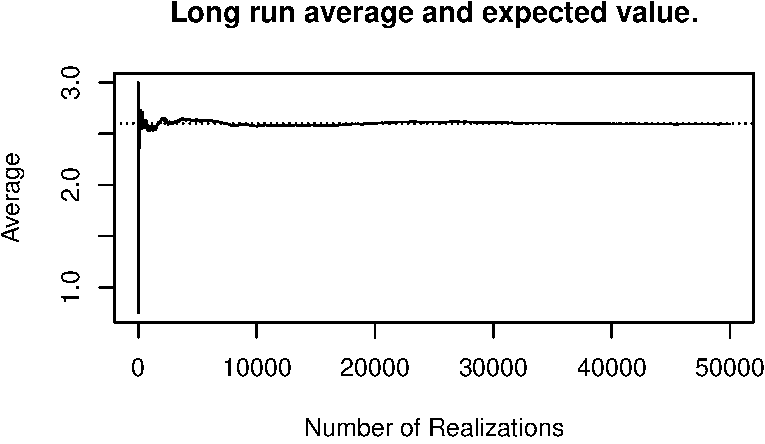
\includegraphics[keepaspectratio]{notes/chapter6_files/figure-pdf/fig-plot-1.pdf}}

}

\end{figure}%

\section{Which Measure of Central Tendency Should be
Used?}\label{which-measure-of-central-tendency-should-be-used}

Where the median demonstrated robustness against extreme values in the
distribution, the mean does not. For instance, if we consider the
distribution of incomes across a particular region, the mean will be
much higher than the median, since those families with exceptionally
high incomes will not be smoothed over as they were with medians. In
this case, the lack of robustness for the expected value will render the
mean a less representative summary for the true behaviour of the random
quantity.

To see this concretely consider a random variable which with equal
probability takes a value between \(1\) and \(9\). This will have
\(E[X] = 5\). Now, if the \(9\) is made to be \(1,000,000\), the
expected value will now be \(E[X] = 111115.\dot1\). This is a far cry
from the median which does not change from \(5\) in either case. This
lack of robustness is desirable in the event of the insurance example
from the median discussion, but will be less desirable in other
settings.

The mean, median, and mode are the three standard measures of central
tendency. They are single values which describe the standard behaviour
of a random quantity. Each of the three has merits as a measure, and
each has drawbacks for certain settings. The question of which to use
and when depends primarily on the question of interest under
consideration, rather than on features of the data alone.\footnote{The
  data is one consideration for which measure to use, but not the only
  one (and not the most important one).} Often, presenting more than one
measure can give a better sense of the distributional behaviour that any
one individual will.

\begin{example}[Charles and Sadie Reflect on the Cupcake
Adventures]\protect\hypertarget{exm-choosing-measure-of-central-tendency}{}\label{exm-choosing-measure-of-central-tendency}

Charles and Sadie decide it is worth stepping back and summarizing all
that has happened with regards to their cupcake adventures, trying to
ensure that distributions are always summarized fairly.

\begin{enumerate}
\def\labelenumi{\alph{enumi}.}
\tightlist
\item
  For the number of sprinkles per cupcake is the mean, median, or mode
  the best measure of central tendency?
\item
  For the amount happiness in customers, is the mean, median, or mode
  the best measure of central tendency?
\item
  For the number of customers who become ill eating at establishments,
  is the mean, median, or mode the best measure of central tendency?
\end{enumerate}

\begin{tcolorbox}[enhanced jigsaw, arc=.35mm, rightrule=.15mm, breakable, bottomrule=.15mm, left=2mm, toprule=.15mm, leftrule=.75mm, opacityback=0, colback=white, colframe=quarto-callout-color-frame]

\vspace{-3mm}\textbf{Solution}\vspace{3mm}

\begin{enumerate}
\def\labelenumi{\alph{enumi}.}
\item
  There is an argument that any of the measures here could work the
  best, it would depend on the individual's preferences. The mode makes
  a lot of sense as, if you are a regular customer, the mode is what you
  will experience day-to-day; most days you will have the modal number
  of sprinkles. The median may make sense as it provides a benchmark for
  measuring what constitutes a lot of sprinkles and a little. Half of
  the time you'll end up with a more sprinkled donut, half the time a
  less. The mean would be particularly interesting to note for the store
  owners themselves, since the mean is directly tied to totals: if the
  store knows that they sell \(100\) cupcakes per day, most days, then
  they also can expect to use \(100\) times the mean number of sprinkles
  in a day. This is helpful for planning.
\item
  The median is likely the most useful measure in this setting. The mode
  could be useful if happiness were not measured on a \(100,000\) point
  scale. The mean is likely a less relevant value here as we are not
  particularly concerned with the total happiness, and if there was a
  large skew or major outliers in this distribution, we would want to
  determine where the majority fall. This is more analogous to the
  income example rather than the insurance example.
\item
  In this case either the mode or mean are likely the best gauges. Here
  we do care about totals, and in particular, we do not want to smooth
  over outliers. It is very relevant if sometimes a lot of individuals
  become ill after eating an establishment, and the median would hide
  this information.
\end{enumerate}

\end{tcolorbox}

\end{example}

Despite the utility of all three measures, the expected value holds a
place of more central importance in probability and statistics. A lot of
this has to do with further mathematical properties of the mean. Because
of its central role, it is worth studying the expected value in some
more depth.

\section{Expected Values of Functions of Random
Variables}\label{expected-values-of-functions-of-random-variables}

Sometimes the value of a random variable needs to be mapped through a
function to give the value which is most relevant to us. Consider, for
instance, a situation wherein the side lengths of boxes being
manufactured by a specific supplier are random, due to incorrectly
calibrated tolerances in the machines. The resulting boxes are perfect
cubes. Suppose we are interested in the volume of the produced box not
the side length. If a box has side length \(x\), then its volume will be
\(x^3\), and so we may desire some way of computing \(E[X^3]\) rather
than \(E[X]\).

Generally, for a function \(g(X)\), we may want to compute \(E[g(X)]\).
It is important to recognize that \(E[g(X)] \neq g(E[X])\). This is a
common mistake.\footnote{and an attractive one, but a mistake
  nonetheless.} If we are unable to apply the function to the expected
value, then the question of how to compute the expected value remains.
Instead of applying the function to overall expected value, instead, we
apply the function to \emph{each} value in the defining relationship for
the expected value. That is,
\[E[g(X)] = \sum_{x\in\mathcal{X}} g(x)p_X(x).\] This is sometimes
referred to as the ``law of the unconscious statistician,'' a name which
may be aggressive enough to help remember the correct way to compute the
expectation.\footnote{Some statisticians dislike this name. I find it to
  be rather cute.}

\begin{tcolorbox}[enhanced jigsaw, arc=.35mm, title={The Law of the Unconscious Statistician}, rightrule=.15mm, coltitle=black, opacitybacktitle=0.6, colbacktitle=quarto-callout-tip-color!10!white, leftrule=.75mm, colback=white, breakable, titlerule=0mm, toptitle=1mm, bottomtitle=1mm, bottomrule=.15mm, toprule=.15mm, opacityback=0, left=2mm, colframe=quarto-callout-tip-color-frame]

The law of the unconscious statistician (LOTUS) states that, for a
random variable \(X\), if we wish to find \(E[g(X)]\), then we compute
\[E[g(X)] = \sum_{x\in\mathcal{X}} g(x)p_X(x).\]

\end{tcolorbox}

\begin{example}[The Happiness Scale
Inversion]\protect\hypertarget{exm-expected-value-transformation}{}\label{exm-expected-value-transformation}

Charles and Sadie have made really great strides working to protect
their favourite coffee shop from the new cupcake store. One day when
digging through the material more, they realize that the happiness
report produced by the company is even less accurate than they had
originally reported! The company reported the following probability mass
function for happiness points \[
p_X(x) = \begin{cases}
    \frac{x}{5,000,050,000} & x \in \{1,\dots,100 000\} \\
    0 & \text{otherwise}.
\end{cases}\] Charles and Sadie track down the source of this expression
and they find that, in fact, this does not measure happiness points at
all. Instead, the number of happiness points is a function of \(X\),
specifically, \(Z = 1/X\).

\begin{enumerate}
\def\labelenumi{\alph{enumi}.}
\tightlist
\item
  What is the expected value of \(X\)? Note, it may be helpful to recall
  that \(\sum_{x=1}^{k} x^2 = \frac{k(k+1)(2k+1)}{6}\).
\item
  What is the expected value of \(Z\)?
\end{enumerate}

\begin{tcolorbox}[enhanced jigsaw, arc=.35mm, rightrule=.15mm, breakable, bottomrule=.15mm, left=2mm, toprule=.15mm, leftrule=.75mm, opacityback=0, colback=white, colframe=quarto-callout-color-frame]

\vspace{-3mm}\textbf{Solution}\vspace{3mm}

\begin{enumerate}
\def\labelenumi{\alph{enumi}.}
\item
  Using directly the formula for \(E[X]\) gives \begin{align*}
  E[X] = \sum_{x=1}^{100000} xp_X(x) &= \sum_{x=1}^{100000} x\frac{x}{5000050000} \\
  &= \frac{1}{5000050000}\sum_{x=1}^{100000}x^2 \\
  &= \frac{1}{5000050000}\cdot\frac{100000(100000+1)(2(100000)+1)}{6} \\
  &= 66 667.
  \end{align*}
\item
  Applying the law of the unconscious statistician, gives \begin{align*}
  E[Z] = E[1/X] = \sum_{x=1}^{100000} \frac{1}{x}p_X(x) &= \sum_{x=1}^{100000} \frac{1}{x}\frac{x}{5000050000} \\
  &= \frac{1}{5000050000}\sum_{x=1}^{100000} 1 \\
  &= \frac{100000}{5000050000} \\
  &= \frac{2}{100001}.
  \end{align*}
\end{enumerate}

\end{tcolorbox}

\end{example}

These functions applied to random variables are often thought of as
``transformations'' of the random quantities. For instance, we
\emph{transformed} a side length into a volume. While the law of the
unconscious statistician will apply to any transformation for a random
variable, we can sometimes use shortcuts to circumvent its application.
In particular, when \(g(X) = aX + b\), for constant numbers \(a\) and
\(b\), we can greatly simplify the expected value of the transformation.
To see this note \begin{align*}
E[aX + b] &= \sum_{x\in\mathcal{X}}(ax + b)p_X(x) \\
&= \sum_{x\in\mathcal{X}}axp_X(x) + bp_X(x) \\
&= a\sum_{x\in\mathcal{X}}xp_X(x) + b\sum_{x\in\mathcal{X}}p_X(X) \\
&= aE[X] + b.
\end{align*} That is, in general, we have that
\(E[aX + b] = aE[X] + b\). Note that part of the property of the
linearity of expectation that we can immediately see if that the
expected value of any constant is always that constant. If we take
\(a = 0\), then we see that \(E[aX + b] = E[b] = b\). Thus, any time
that we need to take the expected value of any constant number, we know
that it is just that number.

This is particularly useful as linear transformations like \(aX+b\)
arise very commonly. For instance, most unit conversions are simple
linear combinations. If a random quantity is measured in one unit then
this result can be used to quickly convert expectations to another.

\begin{example}[Sadie's Trip to
America]\protect\hypertarget{exm-temperature-conversion}{}\label{exm-temperature-conversion}

Sadie has recently returned from a long trip to America. The trip was
long enough that temperatures measured in Fahrenheit started to make
sense. When Sadie and Charles begin to talk about the weather, Charles
brings up the temperature distribution of a possible summer vacation
spot. Unfortunately for Sadie, these temperatures are all in Celsius.
The distribution Charles provides is \[p_X(x) = \begin{cases}
    0.1 & x \in \{10, 11, 12, 13, 14\} \\
    0.05 & x \in \{15, 16, 17, 18, 19, 20, 21, 22, 23, 24\} \\
    0 & \text{otherwise}
\end{cases}\]

\begin{enumerate}
\def\labelenumi{\alph{enumi}.}
\tightlist
\item
  What is the expected temperature, in Celsius?
\item
  Supposing that the temperature in Fahrenheit is given by
  \(Y = 1.8X + 32\), what is the expected temperature in Fahrenheit?
\end{enumerate}

\begin{tcolorbox}[enhanced jigsaw, arc=.35mm, rightrule=.15mm, breakable, bottomrule=.15mm, left=2mm, toprule=.15mm, leftrule=.75mm, opacityback=0, colback=white, colframe=quarto-callout-color-frame]

\vspace{-3mm}\textbf{Solution}\vspace{3mm}

\begin{enumerate}
\def\labelenumi{\alph{enumi}.}
\item
  Here we find \begin{align*}
   \sum_{x=10}^{24} xp_X(x) &= 0.1\sum_{x=10}^{14}x + 0.05\sum_{x=15}^{24}x \\
   &= 15.75.
  \end{align*}
\item
  Since \(E[X] = 15.75\) then
  \(E[Y] = E[1.8X + 32] = 1.8E[X] + 32 = 60.35\).
\end{enumerate}

\end{tcolorbox}

\end{example}

This type of linear transformation also frequently comes up with games
of chance and payouts, or with scoring more generally.\footnote{For
  instance, suppose you are betting a certain amount on the results of a
  coin toss, or that you are taking a multiple choice test that gives
  \(2\) points for a correct answer.} Beyond being linear over simple
transformations, summations in general behave nicely with expectations.
Specifically, for any quantities separated by addition, say
\(g(X) + h(X)\), the expected value will be the sum of each expected
value. Formally, \begin{align*}
E[g(X) + h(X)] &= \sum_{x\in\mathcal{X}} (g(x) + h(x))p_X(x) \\
&= \sum_{x\in\mathcal{X}} g(x)p_X(x) + h(x)p_X(x) \\
&= \sum_{x\in\mathcal{X}} g(x)p_X(x) + \sum_{x\in\mathcal{X}} h(x)p_X(x) \\
&= E[g(X)] + E[h(X)].
\end{align*}

Behaving well under linearity is one of the very nice properties of
expectations. It will come in useful when dealing with a large variety
of important quantities, and as we will see shortly, this linearity will
also extend to multiple different random quantities.

Measures of central tendency are important to summarize the behaviour of
a random quantity. Whether using the mean, median, or mode, these
measures of location describe, on average, what to expect from
observations of the random quantity. However, understanding a
distribution requires understanding far more than simply the measures of
location. As was discussed previously, the probability mass function
captures the complete probabilistic behaviour of a discrete random
variable, it is only intuitive that some information would be lost with
a single numeric summary.

\begin{tcolorbox}[enhanced jigsaw, arc=.35mm, title={Equal Location Across Different Distributions}, rightrule=.15mm, coltitle=black, opacitybacktitle=0.6, colbacktitle=quarto-callout-warning-color!10!white, leftrule=.75mm, colback=white, breakable, titlerule=0mm, toptitle=1mm, bottomtitle=1mm, bottomrule=.15mm, toprule=.15mm, opacityback=0, left=2mm, colframe=quarto-callout-warning-color-frame]

Consider the following three distributions for three random variables,
\(X\), \(Y\), and \(Z\): \begin{align*}
p_X(x) = \begin{cases}
    0.25 & x = -1 \\
    0.5 & x = 0 \\ 
    0.25 & x = 1 \\
    0 & \text{otherwise}.
\end{cases} \quad
p_Y(y) &= \begin{cases}
    0.05 & x = -5 \\
    0.1 & x = -4 \\
    0.1 & x = -3 \\
    0.1 & x = -2\\
    0.1 & x = -1\\
    0.15 & x = 0 \\ 
    0.1 & x = 1\\
    0.1 & x = 2\\
    0.1 & x = 3\\
    0.1 & x = 4 \\
    0.05 & x = 5 \\
    0 & \text{otherwise}.
\end{cases} \quad
p_Z(z) = \begin{cases}
    0.25 & x = -400 \\
    0.5 & x = 0 \\
    \frac{1}{3196} & x \in \{1,\dots,799\}\\
    0 & \text{otherwise}.
\end{cases}.
\end{align*}

In each of these distributions we have the mean, median, and mode all
equalling \(0\).\footnotemark{} However, even just from a quick glance,
these distributions are all very, very differently behaved. The location
summaries here clearly miss much of the important information about
these different distributions. Spend some time trying to think of the
ways in which they differ from one another, and see if you can determine
\emph{what} is missing from relying solely on measures of location.

\end{tcolorbox}

\footnotetext{Try working this out!}

\section{Summarizing the Variability of a Random
Variable}\label{summarizing-the-variability-of-a-random-variable}

A key characteristic of the behaviour of a random variable which is not
captured by the measures of location is the variability of the quantity.
If we imagine taking repeated realizations of a random variable, the
variability of the random variable captures how much movement there will
be observation to observation. If a random variable has low variability,
we expect that the various observations will cluster together, becoming
not too distant from one another. If a random variable has high
variability, we expect the observations to jump around each time.

\subsection{The Range}\label{the-range}

Just as was the case with measures of location, there are several
measures of variability which may be applicable in any given setting.
One fairly basic measure of this variability is the range of possible
values: what is the highest possible value, what is the lowest possible
value, and how much distance is there between those two points?

\begin{definition}[Range]\protect\hypertarget{def-range}{}\label{def-range}

For a random variable, \(X\), the range of the random variable is
defined as \(\text{Range}(X) = \max(X) - \min(X)\). That is, it is the
distance between the maximum value that the random variable can take on,
and the minimum value that the random variable can take on. Sometimes
the range is reported with these outpoints explicitly specified.

\end{definition}

This is a fairly intuitive notion, and is particularly useful in the
equal probability model over a sequence of numbers. Consider dice. Dice
are typically defined by the range of values that they occupy, say \(1\)
to \(6\), or \(1\) to \(20\). Once you know the values present on any
die, you have a sense for how much the values can move observation to
observation.

\begin{example}[Charles and Sadie Explore Ice Cream
Flavors]\protect\hypertarget{exm-range-works}{}\label{exm-range-works}

Charles and Sadie have decided to spend their sunny afternoon exploring
various ice cream flavors at their local parlor, \emph{Symmetric
Scoops}. They notice that Scoops Galore offers a wide variety of
flavors, from classic vanilla to exotic dragon fruit swirl. Intrigued by
the selection, they decide to investigate the probability distribution
of a random variable, \(Y\), representing the number of unique flavors a
customer selects.

After discreetly observing several customers, Charles and Sadie jot down
their findings: \[
p_Y(y) = \begin{cases} 
0.2 & y = 1 \\
0.35 & y = 2 \\
0.3 & y = 3 \\
0.15 & y = 4 \\
0 & \text{otherwise}
\end{cases}
\]

What is the range of the random variable \(Y\), representing the number
of unique ice cream flavors a customer selects at Scoops Galore?

\begin{tcolorbox}[enhanced jigsaw, arc=.35mm, rightrule=.15mm, breakable, bottomrule=.15mm, left=2mm, toprule=.15mm, leftrule=.75mm, opacityback=0, colback=white, colframe=quarto-callout-color-frame]

\vspace{-3mm}\textbf{Solution}\vspace{3mm}

Looking at the defining relationship for this random variable, we can
see that the maximum value the distribution can take on is \(4\) (with
probability \(0.15\)) and the minimum value is \(1\) (with probability
\(0.2\)). As a result, we say that \(\text{Range}(Y) = 4 - 1 = 3\).

\end{tcolorbox}

\end{example}

While the range is an important measure to consider to determine the
behaviour of a random variable, it is a fairly crude measurement. It may
be the case that, while the extreme values are possible, they are
sufficiently unlikely so as to come up very infrequently and not remain
representative of the likely spread of observations. Alternatively, many
random variables have a theoretically infinite range. In these cases,
providing the range will likely not provide much utility.

\begin{example}[Charles and Sadie Explore Ice Cream Flavors,
Again]\protect\hypertarget{exm-range-dnw}{}\label{exm-range-dnw}

Having had so much fun at \emph{Symmetric Scoops} the first time,
Charles and Sadie return once more to continue to investigate customers
behaviour. When they arrive they notice a temporary promotion going on,
which happens on one randomly selected Sunday a year, where customers
can buy a \emph{Mega Sunda(y)e Extravaganza}, a wonderfully extravagant
creation that features scoops from all \(50\) flavours on offer. Working
on this today they find the following probability mass function for
\(Y\). \[
p_Y(y) = \begin{cases} 
0.2 & y = 1 \\
0.35 & y = 2 \\
0.3 & y = 3 \\
0.145 & y = 4 \\
0.005 & y = 50 \\
0 & \text{otherwise}
\end{cases}
\]

What is the range of the random variable \(Y\) now? Does this accurately
represent the dispersion we expect from \(Y\)?

\begin{tcolorbox}[enhanced jigsaw, arc=.35mm, rightrule=.15mm, breakable, bottomrule=.15mm, left=2mm, toprule=.15mm, leftrule=.75mm, opacityback=0, colback=white, colframe=quarto-callout-color-frame]

\vspace{-3mm}\textbf{Solution}\vspace{3mm}

Looking at the defining relationship for this random variable, we can
see that the maximum value the distribution can take on is \(50\) (with
probability \(0.005\)) and the minimum value is \(1\) (with probability
\(0.2\)). As a result, we say that \(\text{Range}(Y) = 50 - 1 = 49\).
This does \textbf{not} accurately represent the dispersion of the random
variable. Not only do very few customers order this when it is
available, it is also almost never available. As a result, the maximum
value (while possible) is not reflective of the usual behaviour of this
random quantity, and this displays one of the concerns with the range as
a measure of spread.

\end{tcolorbox}

\end{example}

\subsection{The Interquartile Range}\label{the-interquartile-range}

To remedy these two issues, we may think of techniques to modify the
range. Instead of taking the minimum and maximum possible values, we can
instead consider ranges of values which remain more plausible. A common
way to do this is to extend our concept of a median beyond the half-way
point. The median of a random variable \(X\), is the value, \(m\), such
that \(P(X \leq m) = 0.5\)\footnote{And, as a result, \(P(X > m) = 0.5\)
  as well.}. While there is good reason to care about the midpoint, we
can think of generalizing this to be \emph{any} probability.

That is, we could find a number \(z\), such that \(P(X \leq z) = 0.1\).
We could then use this value to conclude that the probability of
observing a value less than \(z\) is \(10\%\). These values are referred
to, generally, as \textbf{percentiles} and they are the natural
extension of medians.

\begin{definition}[Percentiles]\protect\hypertarget{def-percentile}{}\label{def-percentile}

The \(100p\)th percentile (e.g., \(70\)th percentile for \(p=0.7\), or
\(20\)th percentile for \(p=0.20\)), is denoted \(\zeta(p)\) and is the
value such that \(P(X \leq \zeta(p)) = p\). Thus, the median is given by
\(\zeta(0.5)\) and is also called the \(50\)th percentile.\footnote{Note
  that, when dealing with discrete random variables, it may not be
  possible to find a value \(\zeta(p)\) such that
  \(P(X \leq \zeta(p)) = p\) exactly. Instead, we typically define the
  percentile here to be such that
  \(P(X < \zeta(p)) < p \leq P(X \leq \zeta(p))\).}

\end{definition}

\begin{example}[Perplexed at the Ice Cream
Parlour]\protect\hypertarget{exm-percentile}{}\label{exm-percentile}

Charles and Sadie remained somewhat disappointed by their lack of
ability to accurately capture the behaviour of a random variable using
the range. To this end, they spend a lot more time at the ice cream
parlor, and come up with, what they believe, is the correct probability
mass function for how many flavours customers order, in total. \[
p_Y(y) = \begin{cases} 
    0.25 & y = 1 \\
    0.25 & y = 2 \\
    0.1 & y = 3 \\
    0.05 & y = 4 \\
    0.05 & y = 5 \\
    0.05 & y = 6 \\
    0.15 & y = 7 \\
    0.05 & y = 8 \\
    0.04 & y = 9 \\
    0.005 & y = 10 \\ 
    0.005 & y = 50 \\
    0 & \text{otherwise}
\end{cases}
\]

Using this probability mass function, find \(\zeta(0.25)\),
\(\zeta(0.5)\), \(\zeta(0.75)\), and \(\zeta(0.99)\). What do each of
these values mean?

\begin{tcolorbox}[enhanced jigsaw, arc=.35mm, rightrule=.15mm, breakable, bottomrule=.15mm, left=2mm, toprule=.15mm, leftrule=.75mm, opacityback=0, colback=white, colframe=quarto-callout-color-frame]

\vspace{-3mm}\textbf{Solution}\vspace{3mm}

\begin{enumerate}
\def\labelenumi{\alph{enumi}.}
\tightlist
\item
  \(\zeta(0.25)\) is found by looking for
  \(P(Y \leq \zeta(0.25)) = 0.25\). We note that
  \(P(Y \leq 1) = P(Y = 1) = 0.25\), and so \(\zeta(0.25) = 1\). This
  means that there is a \(25\%\) chance that a randomly selected
  individual will order \(1\) or fewer flavours.
\item
  \(\zeta(0.5)\) is found by looking for
  \(P(Y \leq \zeta(0.5)) = 0.25\). Note that
  \(P(Y \leq 2) = P(Y = 1) + P(Y = 2) = 0.5\), and so
  \(\zeta(0.5) = 2\). This means that \(50\%\) of customers order \(2\)
  or fewer flavours, and \(50\%\) of customers order more than \(2\)
  flavours.
\item
  \(\zeta(0.75)\) is found by looking for
  \(P(Y \leq \zeta(0.75)) = 0.75\). Note that we can continue the
  cumulative sums from the probability mass function. This gives, in
  order, \(0.25, 0.5, 0.6, 0.65, 0.7, 0.75, 0.9, 0.95, 0.99, 0.995, 1\).
  As a result, \(P(Y \leq 6) = 0.75\) and so \(\zeta(0.75) = 6\). This
  means that \(75\%\) of customers order \(7\) or fewer flavours (the
  remaining \(25\%\) order more than \(7\)).
\item
  \(\zeta(0.99)\) can be found through the same cumulative sums as in
  (c). This is given by \(y = 9\), such that \(P(Y \leq 9) = 0.99\), so
  \(\zeta(0.99) = 9\). This means that \(99\%\) of individuals order
  \(9\) or fewer flavours.
\end{enumerate}

\end{tcolorbox}

\end{example}

We can leverage percentiles to remedy some of the issues with the range
as a measure of variability. Framed in terms of percentiles, the minimum
value is \(\zeta(0)\), and the maximum value is \(\zeta(1)\). Instead of
considering the extreme endpoints, we can consider the difference
between more moderate percentiles. Doing so allows us to overcome the
major concerns outlined with the range. If we take \(\zeta(p_1)\) and
\(\zeta(p_2)\), for \(p_1 < p_2\), then the difference between
\(\zeta(p_2) - \zeta(p_1)\) can be seen as a measure of variability,
analogous to the range.

The most common choices would be to take \(\zeta(0.25)\) and
\(\zeta(0.75)\), the \(25\)th and \(75\)th percentiles, respectively.
These are also referred to as the first and third quartiles,
respectively. They are named as, taking \(\zeta(0.25)\), \(\zeta(0.5)\)
and \(\zeta(0.75)\), the distribution is cut into quarters.

With the first and third quartiles computed, we can compute the
\textbf{interquartile range}, which is given by
\(\zeta(0.75)-\zeta(0.25)\).

\begin{definition}[Interquartile Range
(IQR)]\protect\hypertarget{def-iqr}{}\label{def-iqr}

The interquartile range, or IQR, is defined as
\(\zeta(0.75) - \zeta(0.25)\), the difference between the third and
first quartiles. It is a measure of spread, and is typically denoted as
\(\text{IQR} = Q3 - Q1\), where \(Q\) stands for quartiles.

\end{definition}

Like the range, the IQR gives a measure of how much spread there tends
to be in a distribution. Unlike the range, however, we can be more
certain that both the first and third quartiles are reasonable values
around which repeated observations of the random variable would be
observed. Specifically, there is a probability of \(0.5\) that a value
between the first and third quartile will be observed. The larger the
\(\text{IQR}\), the more spread out these moderate observations will be,
and as a result, the more variable the distribution is.

\begin{example}[Addressing the Ice Cream
Perplexity]\protect\hypertarget{exm-percentile}{}\label{exm-percentile}

Having understood many of the percentiles of the distribution of ice
cream flavours ordered at \emph{Symmetric Scoops}, Charles and Sadie
decide to have another shot at capturing the spread. Recall that the
probability mass function for \(Y\), the number of ice cream flavours
ordered by a customer, is given by \[
p_Y(y) = \begin{cases} 
0.25 & y = 1 \\
0.25 & y = 2 \\
0.1 & y = 3 \\
0.05 & y = 4 \\
0.05 & y = 5 \\
0.05 & y = 6 \\
0.15 & y = 7 \\
0.05 & y = 8 \\
0.04 & y = 9 \\
0.005 & y = 10 \\ 
0.005 & y = 50 \\
0 & \text{otherwise}
\end{cases}
\]

What is the interquartile range for this population? How does this
compare to the range?

\begin{tcolorbox}[enhanced jigsaw, arc=.35mm, rightrule=.15mm, breakable, bottomrule=.15mm, left=2mm, toprule=.15mm, leftrule=.75mm, opacityback=0, colback=white, colframe=quarto-callout-color-frame]

\vspace{-3mm}\textbf{Solution}\vspace{3mm}

We know that \(\zeta(0.25) = 1\) and \(\zeta(0.75) = 6\). As a result,
the \(\text{IQR} = 6 - 1 = 5\). By contrast, the range is given by
\(50 - 1 = 49\). It is incredibly rare to observe a customer ordering
\(50\) flavours, as a result, using \(5\) is a better measure of spread
of the distribution. To see this, we could consider plotting a histogram
(more on these later on) that show the number of customers who order
each type, and then intuitively as for a good measure of how
\emph{spread out} the data are.

\pandocbounded{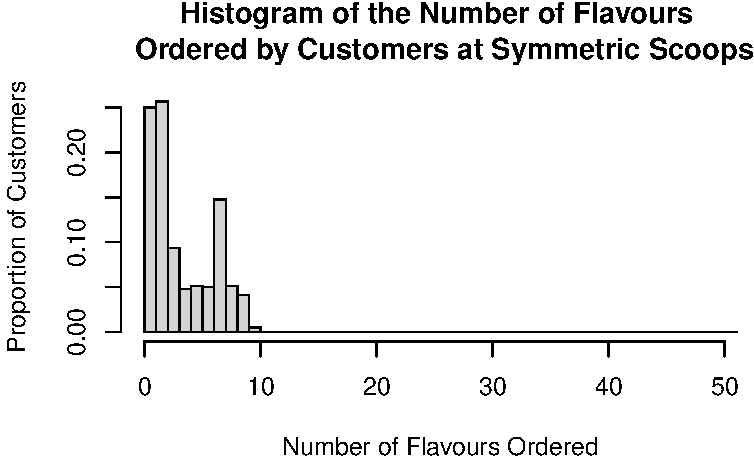
\includegraphics[keepaspectratio]{notes/chapter6_files/figure-pdf/symmetric_scoops_graph-1.pdf}}

\end{tcolorbox}

\end{example}

\subsection{The Variance and Mean Absolute
Deviation}\label{the-variance-and-mean-absolute-deviation}

Both the range and the interquartile range give a sense of the variation
in the distribution irrespective of the measures of location for that
distribution. Another plausible method for assessing the variability of
a distribution is to assess how far we expect observations to be from
its center. Intuitively, if observations of \(X\) are near the center
with high probability, then the distribution will be less variable than
if the average distance to the center is larger.

This intuitive measure of variability is useful for capturing the
behaviour of a random variable, particularly when paired with a measure
of location. However, we do have to be careful: not all measures of
dispersion based on this notion will be useful. Consider the most basic
possibility, \(X - E[X]\). We might ask, for instance, what is the
expected value of this quantity. If we take \(E[X - E[X]]\) then note
that this a linear combination in expectation since \(E[X]\) is just
some number. Thus, \(E[X-E[X]] = E[X] - E[X] = 0\). In other words, the
expected difference between a random variable and its mean is exactly
\(0\). We thus need to think harder about how best to turn this
intuition into a useful measure of spread.

The issue with this procedure is that some realizations are going to be
below the mean, making the difference negative, and some will be above
the mean, making the difference positive. Our defining relationship for
the mean relied on balancing these two sets of mass. However, when
discussing the variability of the random variable, we do not much care
whether the observations are lower than expected or higher than
expected, we simply care how much variability there is around what is
expected. To remedy this, we should consider only the distance between
the observation and the expectation, not the sign. That is, if \(X\) is
\(5\) below \(E[X]\) we should treat that the same as if \(X\) is \(5\)
above \(E[X]\).

There are two common ways to turn value into its magnitude in
mathematics generally: squaring the number and using absolute values.
Both of these tactics are useful approaches to defining measures of
spread, and they result in the \textbf{variance} when using the expected
value of the squared deviations, and the \textbf{mean absolute
deviation} when using the absolute value. While \(E[|X-E[X]|]\) is
perhaps the more intuitive quantity to consider, generally speaking it
will not be the one that we use.

\begin{definition}[Variance]\protect\hypertarget{def-variance}{}\label{def-variance}

The variance of a random variable, typically denoted \(\text{var}(X)\),
is given by the expected value of the squared deviations of a random
variable from its mean. That is,
\[\text{var}(X) = E\left[(X - E[X])^2\right].\]

\end{definition}

\begin{definition}[Mean Absolute
Deviation]\protect\hypertarget{def-MAD}{}\label{def-MAD}

The mean absolute deviation of a random variable, typically denoted
\(\text{MAD}(X)\), is given by the expected value of the absolute value
of the deviations of a random variable from its mean. That is,
\[\text{MAD}(X) = E\left[|X - E[X]|\right].\]

\end{definition}

In general when we need a positive quantity in mathematics it will
typically be preferable to consider the square to the absolute
value.\footnote{The reasons for this are plentiful, but generally
  squares are easier to handle than absolute values, and as a result
  become more natural quantities to consider.} The variance is
\textbf{the} central measure of deviation for random variables. When
discussing the variability of a random variable, it will almost
universally be in reference to the variance.

Note that if we take \(g(X) = (X-E[X])^2\), then the variance of \(X\)
is the expected value of a transformation. We have seen that to compute
these we apply the law of the unconscious statistician, and substitute
\(g(X)\) into the defining relationship for the expected value, which
for the variance gives
\[\text{var}(X) = \sum_{x\in\in\mathcal{X}} (x-E[X])^2p_X(x).\] In order
to compute the variance, we must also find the mean as the function
\(g(X)\) relies upon this value.

\begin{example}[Variation in the Number of Ice Cream Flavours
Ordered]\protect\hypertarget{exm-variance}{}\label{exm-variance}

Noting how different the range and IQR were of the distribution of
number of different flavours ordered by customers at the ice cream
parlour, Charles and Sadie decide to turn to the variance and mean
absolute deviation to try understand the distribution's variability
once-and-for-all. Recall that the probability mass function for \(Y\),
the number of ice cream flavours ordered by a customer, is given by \[
p_Y(y) = \begin{cases} 
0.25 & y = 1 \\
0.25 & y = 2 \\
0.1 & y = 3 \\
0.05 & y = 4 \\
0.05 & y = 5 \\
0.05 & y = 6 \\
0.15 & y = 7 \\
0.05 & y = 8 \\
0.04 & y = 9 \\
0.005 & y = 10 \\ 
0.005 & y = 50 \\
0 & \text{otherwise}
\end{cases}
\]

Find the variance and the mean absolute variation for this distribution.

\begin{tcolorbox}[enhanced jigsaw, arc=.35mm, rightrule=.15mm, breakable, bottomrule=.15mm, left=2mm, toprule=.15mm, leftrule=.75mm, opacityback=0, colback=white, colframe=quarto-callout-color-frame]

\vspace{-3mm}\textbf{Solution}\vspace{3mm}

For both \(\text{var}(Y)\) and \(\text{MAD}(Y)\) we require the expected
value of \(Y\). To this end note that
\begin{multline*}E[Y] = (0.25)(1) + (0.25)(2) + (0.1)(3) + (0.05)(4) + (0.05)(5) + (0.05)(6) + (0.15)(7) \\ + (0.05)(8) + (0.04)(9) + (0.005)(10) + (0.005)(50) = 3.91.\end{multline*}

Then, it can be useful to define a table with the probabilities,
absolute, and squared deviations, so that the summations can be made
easier.

\begin{longtable}[]{@{}cccc@{}}
\toprule\noalign{}
\(Y\) & \(p_Y(y)\) & \((Y - E[Y])^2\) & \(|Y - E[Y]|\) \\
\midrule\noalign{}
\endhead
\bottomrule\noalign{}
\endlastfoot
\(1\) & \(0.25\) & \(8.4681\) & \(2.91\) \\
\(2\) & \(0.25\) & \(3.6481\) & \(1.91\) \\
\(3\) & \(0.1\) & \(0.8281\) & \(0.91\) \\
\(4\) & \(0.05\) & \(0.0081\) & \(0.09\) \\
\(5\) & \(0.05\) & \(1.1881\) & \(1.09\) \\
\(6\) & \(0.05\) & \(4.3681\) & \(2.09\) \\
\(7\) & \(0.15\) & \(9.5481\) & \(3.09\) \\
\(8\) & \(0.05\) & \(16.7281\) & \(4.09\) \\
\(9\) & \(0.04\) & \(25.9081\) & \(5.09\) \\
\(10\) & \(0.005\) & \(37.0881\) & \(6.09\) \\
\(50\) & \(0.005\) & \(2124.2881\) & \(46.09\) \\
\end{longtable}

With this table we can compute both the variance and mean absolute
deviation by taking the second column times by the third, and adding up
those results (for the variance) and the second column times the fourth,
and adding up those results (for the MAD). Doing so results in
\(\text{var}(Y) = 17.5019\) and \(\text{MAD}(Y) = 2.592\).

\end{tcolorbox}

\end{example}

\subsection{Standard Deviation}\label{standard-deviation}

The higher that an individual random variable's variance is, the more
spread we expect there to be in repeated realizations of that quantity.
Specifically, the more spread out around the mean value the random
variable will be. A random variable with a low variance will concentrate
more around its mean value than one with a higher variance. One
confusing part of the variance of a random variable is in trying to
assess the units. Suppose that a random quantity is measured in a
particular set of units -- dollars, seconds, grams, or similar. In this
case, our interpretations of measures of location will all be in the
same units, which aids in drawing connections to the underlying
phenomenon that we are trying to study. However, because the variance is
squared, we cannot make the same extensions to it. Variance is not
measured in the regular units, but in the regular units, \emph{squared}.

Suppose you have a random time being measured, perhaps the reaction time
for some treatment to take effect in a treated patient. Finding the mean
or median will give you a result that you can read off in seconds. The
range and interquartile range both give you the spread in seconds.
However, if you work out the variance of this quantity it will be
measured in seconds squared -- a unit that is challenging to have much
intuition about. To remedy this we will often use a transformed version
of the variance, called the \textbf{standard deviation}, returning the
units to be only the original scale.

\begin{definition}[Standard
Deviation]\protect\hypertarget{def-sd}{}\label{def-sd}

The standard deviation of a random variable is the square root of the
variance, which is to say \[\text{SD}(X) = \sqrt{\text{var}(X)}.\]

\end{definition}

We do not often consider computing the standard deviation directly, and
so will most commonly refer to the variance when discussing the
behaviour of a random variable, but it is important to be able to move
seamlessly between these two measures of spread.

\begin{example}[Variation in the Number of Ice Cream Flavours Ordered,
the Finale]\protect\hypertarget{exm-sd}{}\label{exm-sd}

Having realized that the IQR and range are not directly comparable to
the variance, as they are measured in different units, Charles and Sadie
decide to end their investigation in the variability of the number of
ice cream flavours ordered by calculating the standard deviation of
\(Y\). Recall that the probability mass function for \(Y\), the number
of ice cream flavours ordered by a customer, is given by \[
p_Y(y) = \begin{cases} 
0.25 & y = 1 \\
0.25 & y = 2 \\
0.1 & y = 3 \\
0.05 & y = 4 \\
0.05 & y = 5 \\
0.05 & y = 6 \\
0.15 & y = 7 \\
0.05 & y = 8 \\
0.04 & y = 9 \\
0.005 & y = 10 \\ 
0.005 & y = 50 \\
0 & \text{otherwise}
\end{cases}.
\]

What is the standard deviation of this random variable?

\begin{tcolorbox}[enhanced jigsaw, arc=.35mm, rightrule=.15mm, breakable, bottomrule=.15mm, left=2mm, toprule=.15mm, leftrule=.75mm, opacityback=0, colback=white, colframe=quarto-callout-color-frame]

\vspace{-3mm}\textbf{Solution}\vspace{3mm}

The standard deviation is given by the square root of the variance. This
is given by \(\sqrt{17.5019} = 4.18353\).

\end{tcolorbox}

\end{example}

\begin{example}[The Dolphin
Olympics]\protect\hypertarget{exm-dolphin-olympics}{}\label{exm-dolphin-olympics}

Sadie and Charles, on a trip to a beach in a particularly quirky town,
find themselves watching the \textbf{dolphin Olympics}. These are a set
of games put on by the local dolphin populations where they see how high
they can jump from the water, and how many flips they can do while they
do it. Charles and Sadie get to work determining the probability
distributions related to the heights and the number of flips, with Sadie
taking the heights and Charles taking the number of flips. At the end of
the day they are discussing their findings and Sadie indicates that the
standard deviation of the height that was jumped was \(1.6m\). Charles
is intrigued, saying, ``I could have sworn that there was more variation
in the jump heights than in the number of flips, but the variance of the
flips was \(2.56\), greater than the variability in the heights!''

Is Charles correct? Why or why not?

\begin{tcolorbox}[enhanced jigsaw, arc=.35mm, rightrule=.15mm, breakable, bottomrule=.15mm, left=2mm, toprule=.15mm, leftrule=.75mm, opacityback=0, colback=white, colframe=quarto-callout-color-frame]

\vspace{-3mm}\textbf{Solution}\vspace{3mm}

Charles has compared the standard deviation of the first quantity to the
variance of the second. We must compare the same measure, and as a
result, conclude that the variance of the heights was \(1.6^2 = 2.56\),
exactly the same as the second.

\end{tcolorbox}

\end{example}

\section{Computing the Variance}\label{computing-the-variance}

When computing the variance of a random quantity, we often use a
shortcut for the formula, \[\text{var}(X) = E[X^2] - E[X]^2.\]
Generally, this is moderately more straightforward to calculate since
\(X^2\) is an easier transformation than \((X-E[X])^2\). This identity
will come back time and time again, with a lot of versatility in the
ways that it can be used. Typically, when a variance is needed to be
calculated the process is to simply compute \(E[X]\) and \(E[X^2]\), and
then apply this relationship.

\begin{tcolorbox}[enhanced jigsaw, arc=.35mm, title={Proof of the Variance Identity}, rightrule=.15mm, coltitle=black, opacitybacktitle=0.6, colbacktitle=quarto-callout-warning-color!10!white, leftrule=.75mm, colback=white, breakable, titlerule=0mm, toptitle=1mm, bottomtitle=1mm, bottomrule=.15mm, toprule=.15mm, opacityback=0, left=2mm, colframe=quarto-callout-warning-color-frame]

To determine the variance identity, we need only remember the definition
of the variance (being \(E[(X-E[X])^2]\)), and then use summation
techniques to manipulate the expression. To this end consider,
\begin{align*}
\text{var}(X) &= \sum_{x\in\mathcal{X}} (x-E[X])^2p_X(x) \\
&= \sum_{x\in\mathcal{X}} (x^2 - 2xE[X] + E[X]^2)p_X(x) \\
&=\sum_{x\in\mathcal{X}} x^2p_X(x) - 2E[X]\sum_{x\in\mathcal{X}}xp_X(x) + E[X^2]\sum_{x\in\mathcal{X}}p_X(x)\\
&= E[X^2] - 2E[X]E[X] + E[X]^2\\
&= E[X^2] - E[X]^2.
\end{align*}

\end{tcolorbox}

\begin{example}[Choosing the Outcome of a
Die]\protect\hypertarget{exm-var-calc}{}\label{exm-var-calc}

Charles and Sadie come across a new game of chance involving the rolling
of a die. In it a player chooses a number between \(1\) and \(6\). They
then roll a die (up to) \(6\) times. If they get their chosen number on
the first throw for the first time, they get \(\$1\). If they get their
chosen number on the second throw, they get \(\$2\). The same goes for
the first time seeing their chosen number from throws \(3\) through
\(6\). If they never get the chosen number, they have to pay \(\$1\).

What is the expected value and variance of a player playing this game?

\begin{tcolorbox}[enhanced jigsaw, arc=.35mm, rightrule=.15mm, breakable, bottomrule=.15mm, left=2mm, toprule=.15mm, leftrule=.75mm, opacityback=0, colback=white, colframe=quarto-callout-color-frame]

\vspace{-3mm}\textbf{Solution}\vspace{3mm}

Let \(X\) represent the winnings of a play of this game. We know that
\(X\) takes a value in \(\{-1, 1, 2, 3, 4, 5, 6\}\). The \(p_X(-1)\) is
given by the probability that the die never shows the chosen number. We
can view this as \(6\) independent trials, where each trial is the
result of a die roll. If \(A_j\) is the event that the die shows the
selected number, then we can calculate
\(P(A_1^C, A_2^C, A_3^C, A_4^C, A_5^C, A_6^C) = P(A_1^C)P(A_2^C)P(A_3^C)P(A_4^C)P(A_5^C)P(A_6^C)\).
Note that each of these probabilities is equivalent, and equivalently
equal to \(\dfrac{5}{6}\), and so this probability is
\(\left(\dfrac{5}{6}\right)^6 \approx 0.335\). The remainder of the
outcomes happen if the first time that the number shows up is on toss
\(j\). This means that we have \(A_1, \dots, A_{j-1}^C\) and then
\(A_j\) occurring. As a result, for \(j=1,\dots,6\) we get
\(P(A_1^C, \dots, A_{j-1}^C, A_j) = P(A_1^C)^{j-1}P(A_j)\). Note that
\(P(A_j) = \dfrac{1}{6}\), no matter \(j\), and so the total probability
here is \(\left(\dfrac{5}{6}\right)^{j-1}\left(\dfrac{1}{6}\right)\).
This fully defines the probability mass function.

To get the \(E[X]\) we can apply the standard expectation formula. To
get the variance we can note that \(\text{var}(X) = E[X^2] - E[X]^2\),
and so while we compute \(E[X]\) we can also compute \(E[X^2]\). To this
end
\[E[X] = (-1)\left(\frac{5}{5}\right)^6 + \frac{1}{6}\left[1 + 2\left(\frac{5}{6}\right) + 3\left(\frac{5}{6}\right)^{2} + 4\left(\frac{5}{6}\right)^{3} + 5\left(\frac{5}{6}\right)^{4}+ 6\left(\frac{5}{6}\right)^{5}\right].\]
Solving this gives approximately \(\$0.98\), so every play of the game
you would expect to earn \(98\) cents, approximately. To find
\(E[X^2]\), we use essentially the same setup, this time squaring the
values,
\[E[X] = (-1)^2\left(\frac{5}{5}\right)^6 + \frac{1}{6}\left[1^2 + 2^2\left(\frac{5}{6}\right) + 3^2\left(\frac{5}{6}\right)^{2} + 4^2\left(\frac{5}{6}\right)^{3} + 5^2\left(\frac{5}{6}\right)^{4}+ 6^2\left(\frac{5}{6}\right)^{5}\right].\]
This is \(8.728\), approximately. Then the variance will be given by
\[\text{var}(X) = E[X^2] - E[X]^2 \approx 8.728 - (0.98)^2 = 7.7676.\]

\end{tcolorbox}

\end{example}

\section{The Variance of
Transformations}\label{the-variance-of-transformations}

With expectations, we saw that \(E[g(X)]\) needed to be directly
computed from the definition. The same is true for variances of
transformations. Specifically, \(\text{var}(g(X))\) is given by
\(E[(g(X) - E[g(X)])^2]\) which can be simplified with the previous
relationship as \(E[g(X)^2] - E[g(X)]^2\). Just as with expectations, it
is important to realize that \(\text{var}(g(X)) \neq g(\text{var}(X))\),
and so dealing with transformations requires further work.

With expectations, we highlighted linear transformations as a special
case, with \(g(X) = aX + b\). For the variance, the linear
transformations are also worth distinguishing from others. In
particular, \[\text{var}(aX + b) = a^2\text{var}(X).\] In the same way
that the linearity of expectation demonstrates that the expected value
of any constant is that constant, we can use this identity to show that
the variance of constant is zero. However, we can also reason to this
based on our definitions so far. Suppose that we have a random variable
which is constant.\footnote{This seems to be an oxymoron, but it is
  perfectly well defined.} A constant \(b\) can be seen as a random
variable with probability distribution \(p_X(x) = 1\) if \(x=b\) and
\(p_X(x) = 0\) otherwise. The expected value is going to be
\(E[X] = 1(b) = b\), and \(E[X^2] = 1(b)^2 = b^2\). Thus,
\(\text{var}(b) = E[X^2] - E[X]^2 = b^2 - b^2 = 0\). From an intuitive
perspective, there is no variation around the mean of a constant. It is
always the same value. As a result, when taking the variance, we know
that it should be \(0\).

\begin{tcolorbox}[enhanced jigsaw, arc=.35mm, title={Proof of the Variance of Linear Transformations}, rightrule=.15mm, coltitle=black, opacitybacktitle=0.6, colbacktitle=quarto-callout-warning-color!10!white, leftrule=.75mm, colback=white, breakable, titlerule=0mm, toptitle=1mm, bottomtitle=1mm, bottomrule=.15mm, toprule=.15mm, opacityback=0, left=2mm, colframe=quarto-callout-warning-color-frame]

To calculate the variance of a linear transformation of a random
variable we can apply the standard identity for the variance, giving
\begin{align*}
E[(aX+b)^2] &= E[a^2X^2 + 2abX + b^2] \\
&= E[a^2X^2] + E[2abX] + E[b^2]\\
&= a^2E[X^2] + 2abE[X] + b^2.
\end{align*} Next, we note that \(E[aX + b] = aE[X] + b\) and so
\begin{align*}
E[aX + b]^2 &= (aE[X] + b)^2 \\
&= a^2E[X]^2 + 2abE[X] + b^2.\end{align*} Differencing these two
quantities gives
\[a^2E[X^2] + 2abE[X] + b^2 - a^2E[X]^2 - 2abE[X] - b^2 = a^2(E[X^2] - E[X]^2).\]
By noting that \(E[X^2] - E[X]^2\), we can complete the statement that
\[\text{var}(aX + b) = a^2\text{var}(X).\]

\end{tcolorbox}

Thus, when applying a linear transformation, only the multiplicative
constant matters, and it transforms the variance by a squared factor.
This should make some intuitive sense that the additive constant does
not change anything. If we consider that variance is a measure of
spread, adding a constant value to our random quantity will not make it
more or less spread out, it will simply shift where the spread is
located. This is not true of the mean, which measures where the center
of the distribution is, which helps explain why the result identities
are different.

\begin{example}[Sadie's Trip to
America]\protect\hypertarget{exm-var-linear-transformation}{}\label{exm-var-linear-transformation}

When Sadie had recently returned from a long trip to America, Charles
and Sadie worked out how to convert the expected values of temperatures
from Celsius to Fahrenheit. They now wish to do the same, with the
variances. The distribution of daily temperatures, in Celsius, is
\[p_X(x) = \begin{cases}
    0.1 & x \in \{10, 11, 12, 13, 14\} \\
    0.05 & x \in \{15, 16, 17, 18, 19, 20, 21, 22, 23, 24\} \\
    0 & \text{otherwise}
\end{cases}\]

\begin{enumerate}
\def\labelenumi{\alph{enumi}.}
\tightlist
\item
  What is the variance of temperatures, in Celsius?
\item
  Supposing that the temperature in Fahrenheit is given by
  \(Y = 1.8X + 32\), what is the variance of temperatures in Fahrenheit?
\end{enumerate}

\begin{tcolorbox}[enhanced jigsaw, arc=.35mm, rightrule=.15mm, breakable, bottomrule=.15mm, left=2mm, toprule=.15mm, leftrule=.75mm, opacityback=0, colback=white, colframe=quarto-callout-color-frame]

\vspace{-3mm}\textbf{Solution}\vspace{3mm}

\begin{enumerate}
\def\labelenumi{\alph{enumi}.}
\item
  Here we find \begin{align*}
   E[X] = \sum_{x=10}^{24} xp_X(x) &= 0.1\sum_{x=10}^{14}x + 0.05\sum_{x=15}^{24}x \\
   &= 15.75. \\
   E[X^2] = \sum_{x=10}^{24} x^2p_X(x) &= 0.1\sum_{x=10}^{14}x^2 + 0.05\sum_{x=15}^{24}x^2 \\
   &= 267.25 \\
   \text{var}(X) &= 267.25 - 15.75^2 \\
   &= 19.1875.
  \end{align*}
\item
  Since \(\text{var}(X) = 19.1875\), then we know that
  \(\text{var}(Y) = \text{var}(1.8X + 32) = 1.8^2\text{var}(X) = 62.1675\).
\end{enumerate}

\end{tcolorbox}

\end{example}

Unlike the expectation, the variance of additive terms will not
generally be the addition of the variances themselves. That is, we
cannot say that
\(\text{var}(g(X) + h(X)) = \text{var}(g(X)) + \text{var}(h(X))\).
Writing out the definition shows issue with this,
\[E[(g(X) + h(X))^2] = E[g(X)^2] + 2E[g(X)h(X)] + E[h(X)^2].\] The first
and third terms here are nicely separated and behave well. However, the
central term is not generally easy to simplify. You can view
\(g(X)h(X)\) as a function itself, and so
\[E[g(X)h(X)] \neq E[g(X)]E[h(X)].\] Instead, this will typically need
to be worked out for any specific set of functions.

\section*{Exercises}\label{exercises-4}
\addcontentsline{toc}{section}{Exercises}

\markright{Exercises}

\begin{exercise}[]\protect\hypertarget{exr-6.1}{}\label{exr-6.1}

Find the variance and standard deviation of the sum obtained in tossing
a pair of standard dice.

\end{exercise}

\begin{exercise}[]\protect\hypertarget{exr-6.2}{}\label{exr-6.2}

In a lottery there are \(200\) prizes of \(\$5\), \(20\) prizes of
\(\$25\), and \(5\) prizes of \(\$100\). Assuming that \(10,000\)
lottery tickets are to be issued and sold, what is the fair prices to
pay for a ticket?

\end{exercise}

\begin{exercise}[]\protect\hypertarget{exr-6.3}{}\label{exr-6.3}

Suppose that \(X\) is a random variable with mean \(9.5\) and variance
\(0.16\). For each of the following, identify whether you can determine
the mean and variance of the listed quantity, and if so, find it.

\begin{enumerate}
\def\labelenumi{\alph{enumi}.}
\tightlist
\item
  \(3X\).
\item
  \(2X + 4\).
\item
  \(X^2\).
\item
  \(\frac{X^3}{X^2}\).
\end{enumerate}

\end{exercise}

\begin{exercise}[]\protect\hypertarget{exr-6.4}{}\label{exr-6.4}

Consider the following pmf. \[
p(x) = \begin{cases}
        \frac{1}{5} & X \in \{0, 1, 2\} \\
        \frac{1}{10} & X \in \{3, 4\} \\
        \frac{1}{15} & X \in \{5, 6, 7\} \\
        0 & \text{otherwise}.
    \end{cases}
\]

Calculate:

\begin{enumerate}
\def\labelenumi{\alph{enumi}.}
\tightlist
\item
  \(E[X]\).
\item
  \(\text{var}(X)\).
\item
  \(\zeta(0.5)\).
\item
  \(\text{Range}(X)\).
\item
  \(\text{MAD}(X)\).
\item
  \(E[X^3]\).
\item
  \(\text{var}(X^3)\).
\item
  \(E[2X + 3X^2]\).
\item
  \(\text{var}(e^X)\).
\end{enumerate}

\end{exercise}

\begin{exercise}[]\protect\hypertarget{exr-6.5}{}\label{exr-6.5}

Peter and Paula play a game of chance that consists of several rounds.
Each individual round is won, with equal probabilities of \(1/2\), by
either Peter or Paula; the winner then receives one point. Successive
rounds are independent. Each has staked \$50 for a total of \$100, and
they agree that the game ends as soon as one of them has won a total of
5 points; this player then receives the \$100. After they have completed
four rounds, of which Peter has won three and Paula only one, a fire
breaks out so that they cannot continue their game.

\begin{enumerate}
\def\labelenumi{\alph{enumi}.}
\tightlist
\item
  How should the \$100 be divided between Peter and Paula?
\item
  How should the \$100 be divided in the general case, when Peter needs
  to win \(a\) more rounds and Paula needs to win \(b\) more rounds?
\end{enumerate}

\end{exercise}

\begin{exercise}[]\protect\hypertarget{exr-6.6}{}\label{exr-6.6}

Suppose that \(X\) is a random variable with mean \(\mu\) and variance
\(\sigma^2\). Prove that \[Z=\frac{X-\mu}{\sigma},\] is a random
variable with mean \(0\) and variance \(1\).

\end{exercise}

\begin{exercise}[]\protect\hypertarget{exr-6.7}{}\label{exr-6.7}

Describe several measures of location indicating the strengths and
drawbacks of each.

\end{exercise}

\begin{exercise}[]\protect\hypertarget{exr-6.8}{}\label{exr-6.8}

Describe several measures of variability indicating the strengths and
drawbacks of each.

\end{exercise}

\begin{exercise}[]\protect\hypertarget{exr-6.9}{}\label{exr-6.9}

~

\begin{enumerate}
\def\labelenumi{\alph{enumi}.}
\tightlist
\item
  Suppose that two random quantities have the same mode, median, and
  expected value. Is their distribution guaranteed to be the same? Is it
  guaranteed to be similar? Why?
\item
  Suppose that two random quantities have the same range, IQR, variance,
  and mean absolute deviation. Is their distribution guaranteed to be
  the same? Is it guaranteed to be similar? Why?
\item
  Suppose that two random quantities have the same percentiles for all
  values for which the percentiles are defined. Is their distribution
  guaranteed to be teh same? Is it guaranteed to be similar? Why?
\end{enumerate}

\end{exercise}

\begin{exercise}[]\protect\hypertarget{exr-6.10}{}\label{exr-6.10}

Is it possible for a random variable, which only takes on positive
values, to have a standard deviation which is larger than its mean?
Explain.

\end{exercise}

\begin{exercise}[]\protect\hypertarget{exr-6.11}{}\label{exr-6.11}

Is it possible to, knowing that \(\text{var}(X) > \text{var}(Y)\),
conclude anything regarding \(\text{MAD}(X)\) and \(\text{MAD}(Y)\)?
Explain.

\end{exercise}

\begin{exercise}[]\protect\hypertarget{exr-6.12}{}\label{exr-6.12}

Consider a bag containing three red marbles, two green marbles, and four
blue marbles. You randomly draw two marbles without replacement. Let
\(Y\) represent the number of green marbles drawn.

The probability mass function is given by, \[
p_Y(y) = \begin{cases} 
\frac{31}{36} & y = 0 \\
\frac{14}{36} & y = 1 \\
\frac{1}{36} & y = 2 \\
0 & \text{otherwise}
\end{cases}
\]

\begin{enumerate}
\def\labelenumi{\alph{enumi}.}
\tightlist
\item
  What is the expected value of \(X\)?
\item
  What is the mode of \(X\)?
\item
  What is the variance of \(X\)?
\item
  What is the range of \(X\)?
\item
  What is the standard deviation of \(X\)?
\end{enumerate}

\end{exercise}

\begin{exercise}[]\protect\hypertarget{exr-6.13}{}\label{exr-6.13}

Suppose you toss a biased coin three times. Let \(Z\) represent the
number of heads obtained.

The probability mass function is given by, \[
p_Z(z) = \begin{cases} 
\frac{1}{8} & z = 0 \\
\frac{3}{8} & z = 1 \\
\frac{3}{8} & z = 2 \\
\frac{1}{8} & z = 3 \\
0 & \text{otherwise}
\end{cases}
\]

\begin{enumerate}
\def\labelenumi{\alph{enumi}.}
\tightlist
\item
  What is the expected value of \(X\)?
\item
  What is the median of \(X\)?
\item
  What is the variance of \(X\)?
\item
  What is the standard deviation of \(X\)?
\end{enumerate}

\end{exercise}

\begin{exercise}[]\protect\hypertarget{exr-6.14}{}\label{exr-6.14}

Suppose you observe the number of cars passing a traffic light in a
minute. Let \(W\) represent the number of cars observed.

The probability mass function is given by, \[
p_W(w) = \begin{cases} 
\frac{1}{10} & w = 0 \\
\frac{2}{10} & w = 1 \\
\frac{3}{10} & w = 2 \\
\frac{2}{10} & w = 3 \\
\frac{1}{10} & w = 4 \\
0 & \text{otherwise}
\end{cases}
\]

\begin{enumerate}
\def\labelenumi{\alph{enumi}.}
\tightlist
\item
  What is the expected value of \(X\)?
\item
  What is the mode of \(X\)?
\item
  What is the variance of \(X\)?
\item
  What is \(\zeta(0.3)\)?
\item
  What is \(\zeta(0.8)\)?
\item
  What is the standard deviation of \(X\)?
\end{enumerate}

\end{exercise}

\begin{exercise}[]\protect\hypertarget{exr-6.15}{}\label{exr-6.15}

Consider a book containing 200 pages. You randomly select a page number.
Let \(X\) represent the sum of the digits in the page number selected.

\begin{enumerate}
\def\labelenumi{\alph{enumi}.}
\tightlist
\item
  What is the expected value of \(X\)?
\item
  What is the variance of \(X\)?
\item
  What is the range of \(X\)?
\item
  What is the standard deviation of \(X\)?
\end{enumerate}

\end{exercise}

\chapter{Expectations and Variances with Multiple Random
Variables}\label{expectations-and-variances-with-multiple-random-variables}

\section{Conditional Expectation}\label{conditional-expectation}

Up until this point we have considered the marginal probability
distribution when exploring the measures of central tendency and spread.
These help to summarize the marginal behaviour of a random quantity,
capturing the distribution of \(X\) alone. When introducing
distributions, we also made a point to introduce the conditional
distribution as one which is particularly relevant when there is extra
information. The question ``what do we expect to happen, given that we
have an additional piece of information?'' is not only well-defined, but
it is an incredibly common type of question to ask.\footnote{For
  instance, you might ask ``how long do we expect a patient to live,
  given that they received a particular treatment?'' or ``how much do we
  expect this house to sell for, given it has a certain square
  footage?'' or ``how many goals do we expect this hockey team to score,
  given their current lineup?'' A large number of questions which we may
  hope to answer using data can be framed as a question of conditional
  expectation.} To answer it, we require \textbf{conditional
expectations}.

\begin{definition}[]\protect\hypertarget{def-conditional-expectation}{}\label{def-conditional-expectation}

The conditional expectation of a random variable, \(X\), given a second
random variable, \(Y\), is the average value of \(X\) when we know the
value of \(Y\). Specifically, we write \(E[X|Y]\), and define this to be
\[E[X|Y] = \sum_{x\in\mathcal{X}} xp_{X|Y}(x|y),\] which is exactly
analogous to the defining relationship for \(E[X]\), replacing the
marginal probability mass function with the conditional probability mass
function.

\end{definition}

In principle, a conditional expectation is no more challenging to
calculate than a marginal expectation. Suppose we want to know the
expected value of \(X\) assuming that we know that a second random
quantity, \(Y\) has taken on the value \(y\). We write this as
\(E[X|Y=y]\), and we replace \(p_X(x)\) with \(p_{X|Y}(x|y)\) in the
defining relationship. That is
\[E[X|Y=y] = \sum_{x\in\mathcal{X}}xp_{X|Y}(x|y).\] We can think of the
conditional distribution of \(X|Y=y\) as simply being a distribution
itself, and then work with that no differently. The conditional
variance, which we denote \(\text{var}(X|Y=y)\) is defined in an exactly
analogous manner, giving \[\text{var}(X|Y) = E[(X - E[X|Y])^2|Y].\]

Above we supposed that we knew that \(Y=y\). However, sometimes we want
to work with the conditional distribution more generally. That is, we
want to investigate the behaviour of \(X|Y\), without yet knowing what
\(Y\) equals. We can use the same procedure as above, however, this time
we leave \(Y\) unspecified. We denote this as \(E[X|Y]\), and this
expression will be a function of \(Y\). Then, whenever a value for \(Y\)
is observed, we can specify \(Y=y\), deriving the specific value. We
will typically compute \(E[X|Y]\) rather than \(E[X|Y=y]\), since once
we have \(E[X|Y]\) we can easily find \(E[X|Y=y]\) for \emph{every}
value of \(y\).

\begin{example}[Charles Commences
Crocheting]\protect\hypertarget{exm-conditional-expectation}{}\label{exm-conditional-expectation}

Charles has recently taking up crocheting, but as it is a new skill, is
still in the phase of learning where mistakes are somewhat common. When
sitting down to practice, the number of rows that Charles can complete
in an hour is being recorded by Sadie, as a random quantity \(X\). After
these have been completed, Charles goes back through and counts the
number of mistakes that were made, recording this as \(Y\). In their
experiments they find that
\[p_{X,Y}(x,y) = \frac{44800}{854769} \frac{1}{(x-y)!y!} \left(\frac{21}{10}\right)^x\left(\frac{3}{7}\right)^{y}, \]
for \(x \in \{1,2,3,\dots,10\}\) and \(y \in\{0,1,2,\dots,y\}\). Sadie
works out that
\[p_X(x) = \frac{44800}{854769} \frac{3^x}{x!}, \quad x\in\{1,2,3,\dots,10\}.\]

\begin{enumerate}
\def\labelenumi{\alph{enumi}.}
\tightlist
\item
  How could Sadie have worked out \(p_X(x)\)? You do not need to
  actually compute it.
\item
  If we know that \(X = 3\), what is the expected value of \(Y\)?
\item
  Generally, given \(X\), write down an expression for the expected
  value of \(Y\).
\item
  \textbf{Challenge:} Can you simplify the expression in (c)? It may be
  useful to know that \(k\dbinom{n}{k} = n\dbinom{n-1}{k-1}\).
\item
  What is the variance of \(Y\), when \(X=3\)?
\end{enumerate}

\begin{tcolorbox}[enhanced jigsaw, arc=.35mm, rightrule=.15mm, breakable, bottomrule=.15mm, left=2mm, toprule=.15mm, leftrule=.75mm, opacityback=0, colback=white, colframe=quarto-callout-color-frame]

\vspace{-3mm}\textbf{Solution}\vspace{3mm}

\begin{enumerate}
\def\labelenumi{\alph{enumi}.}
\tightlist
\item
  Sadie could have used the process of marginalization. That is,
  \[p_X(x) = \sum_{y = 0}^{x} p_{X,Y}(x,y) = \sum_{y=0}^{x} \frac{44800}{854769} \frac{1}{(x-y)!y!} \left(\frac{21}{10}\right)^x\left(\frac{3}{7}\right)^{y}.\]
\item
  We want \(E[Y|X=3]\). For this, we can use \(p_{Y|X}(y|3)\) as the
  distribution, which is expressible as
  \[p_{Y|X}(y|3) = \frac{\frac{44800}{854769} \frac{1}{(3-y)!y!} \left(\frac{21}{10}\right)^3\left(\frac{3}{7}\right)^{y}}{\frac{44800}{854769} \frac{3^{3}}{(3)!}} = \left(\frac{7}{10}\right)^3\binom{3}{y}\left(\frac{3}{7}\right)^y,\]
  where \(y \in \{0,1,2,3\}\). Then, \begin{align*}
   E[Y|X=3] &= \sum_{y=0}^3 y\left(\frac{7}{10}\right)^3\binom{3}{y}\left(\frac{3}{7}\right)^y \\
   &= (1)\left(\frac{7}{10}\right)^3\binom{3}{1}\left(\frac{3}{7}\right)^1 + (2)\left(\frac{7}{10}\right)^3\binom{3}{2}\left(\frac{3}{7}\right)^2 + (3)\left(\frac{7}{10}\right)^3\binom{3}{3}\left(\frac{3}{7}\right)^3 \\
   &= \frac{9}{10} = 0.9.
  \end{align*}
\item
  Following the same process as above, we first get that the general
  conditional distribution is given by
  \[p_{Y|X}(y|x) = \frac{\frac{44800}{854769} \frac{1}{(x-y)!y!} \left(\frac{21}{10}\right)^x\left(\frac{3}{7}\right)^{y}}{\frac{44800}{854769} \frac{3^{x}}{(x)!}} = \binom{x}{y}\left(\frac{7}{10}\right)^x\left(\frac{3}{7}\right)^y,\]
  for \(y\in\{0,\dots,x\}\). Then the expected value of \(E[Y|X]\) can
  be found as \begin{align*}
  E[Y|X] &= \sum_{y=0}^x y\binom{x}{y}\left(\frac{7}{10}\right)^x\left(\frac{3}{7}\right)^y.
  \end{align*}
\item
  We have \begin{align*}
  E[Y|X] &= \sum_{y=0}^x y\binom{x}{y}\left(\frac{7}{10}\right)^x\left(\frac{3}{7}\right)^y \\
  &= \sum_{y=1}^x y\binom{x}{y}\left(\frac{7}{10}\right)^x\left(\frac{3}{7}\right)^y \\
  &= \sum_{y=1}^x x\binom{x-1}{y-1}\left(\frac{7}{10}\right)^x\left(\frac{3}{7}\right)^y \\
  &= \frac{3x}{10}\sum_{y=1}^x \binom{x-1}{y-1}\left(\frac{7}{10}\right)^{x-1}\left(\frac{3}{7}\right)^{y-1} \\
  &= \frac{3x}{10}\sum_{k=0}^{r} \binom{r}{k}\left(\frac{7}{10}\right)^r\left(\frac{3}{7}\right)^{k} \\
  &= \frac{3x}{10}\sum_{k=0}^{r} p_{Y|X}(k|r) \\
  &= \frac{3x}{10}.
  \end{align*}
\item
  We have seen that \(E[Y|X=3] = 0.9\). As a result, using the
  previously derived conditional probability distribution,
  \begin{align*}
   \text{var}(Y|X=3) &= \sum_{y=0}^3 (y-0.9)^2\left(\frac{7}{10}\right)^3\binom{3}{y}\left(\frac{3}{7}\right)^y \\
   &= 0.9^2\left(\frac{7}{10}\right)^3\binom{3}{0}\left(\frac{3}{7}\right)^0 + (0.1)^2\left(\frac{7}{10}\right)^3\binom{3}{1}\left(\frac{3}{7}\right)^1 \\
   &\quad + (1.1)^2\left(\frac{7}{10}\right)^3\binom{3}{2}\left(\frac{3}{7}\right)^2 + (2.1)^2\left(\frac{7}{10}\right)^3\binom{3}{3}\left(\frac{3}{7}\right)^3 \\
   &= 0.63
  \end{align*}
\end{enumerate}

\end{tcolorbox}

\end{example}

\section{Conditional Expectations as Random
Variables}\label{conditional-expectations-as-random-variables}

Since \(E[X|Y]\) is a function of an unknown random quantity, \(Y\),
\(E[X|Y]\) is also a random variable.\footnote{It is useful to keep in
  mind that anytime we do \emph{anything} with a random variable,
  mathematically, we produce an additional random variable. If we think
  of a random variable as being some mathematical variable whose value
  depends on the results of an experiment, then if we take that value
  and apply a function to it we have a \emph{new} value whose results
  also depend on the results of an experiment.} It is a transformation
of \(Y\), and as such, it will have some distribution, some expectation,
and some variance itself. This is often a confusing concept when it is
first introduced, so to recap:

\begin{itemize}
\tightlist
\item
  \(X\) and \(Y\) are both random variables;
\item
  \(E[X]\) and \(E[Y]\) are both constant, numerical values describing
  the distribution of \(X\) and \(Y\);
\item
  \(E[X|Y=y]\) and \(E[Y|X=x]\) are each numeric constants which
  summarize the distribution of \(X|Y=y\) and \(Y|X=x\) respectively;
\item
  \(E[X|Y]\) and \(E[Y|X]\) are functions of \(Y\) and \(X\),
  respectively, and can as such be seen as transformations of (and
  random quantities depending on) \(Y\) and \(X\) respectively.
\end{itemize}

We do not often think of the distribution of \(E[X|Y]\) directly,
however, there are very useful results regarding its expected value and
its variance, which will commonly be exploited. If we take the expected
value of \(E[X|Y]\) we will find that \(E[E[X|Y]] = E[X]\). Note that
since \(E[X|Y] = g(Y)\) for some transformation, \(g\), the outer
expectation is taken with respect to the distribution of \(Y\).
Sometimes when this may get confusing we will use notation to emphasize
this fact, specifically, \(E_Y[E_{X|Y}[X|Y]] = E_X[X]\). This notation
is not necessary, but it can clarify when there is much going on, and is
a useful technique to fallback on.

\begin{tcolorbox}[enhanced jigsaw, arc=.35mm, title={The Law of Total Expectation}, rightrule=.15mm, coltitle=black, opacitybacktitle=0.6, colbacktitle=quarto-callout-tip-color!10!white, leftrule=.75mm, colback=white, breakable, titlerule=0mm, toptitle=1mm, bottomtitle=1mm, bottomrule=.15mm, toprule=.15mm, opacityback=0, left=2mm, colframe=quarto-callout-tip-color-frame]

For any random quantities, \(X\) and \(Y\), the Law of Total Expectation
states that \[E[X] = E[E[X|Y]].\] That is, if we first compute the
conditional expectation of \(X\) given \(Y\), then take the expected
value of this quantity, we compute \(E[X]\).

\end{tcolorbox}

In the same way that it is sometimes easier to first condition on \(Y\)
in order to compute the marginal distribution of \(X\) via applications
of the law of total probability, so too can it be easier to first work
out conditional expectations, and then take the expected value of the
resulting expression.

\begin{tcolorbox}[enhanced jigsaw, arc=.35mm, title={Proof of the Law of Total Expectation}, rightrule=.15mm, coltitle=black, opacitybacktitle=0.6, colbacktitle=quarto-callout-warning-color!10!white, leftrule=.75mm, colback=white, breakable, titlerule=0mm, toptitle=1mm, bottomtitle=1mm, bottomrule=.15mm, toprule=.15mm, opacityback=0, left=2mm, colframe=quarto-callout-warning-color-frame]

To prove that law of total expectation, we note that \(E[X|Y]\) is a
random function of \(Y\). As a result, we can apply the LOTUS to
\(E[X|Y]\) as a function of \(Y\) when we take \(E[E[X|Y]]\). Doing so
yields, \begin{align*}
E_Y[E[X|Y]] &= \sum_{y\in\mathcal{Y}} E[X|Y]p_Y(y) \\
&= \sum_{y\in\mathcal{Y}}\left(\sum_{x\in\mathcal{X}}xp_{X|Y}(x|Y)\right)p_Y(y) \\
&= \sum_{y\in\mathcal{Y}}\sum_{x\in\mathcal{X}}x\frac{p_{X,Y}(x,y)}{p_Y(y)}p_Y(y)\\
&= \sum_{x\in\mathcal{X}}\sum_{y\in\mathcal{Y}}xp_{X,Y}(x,y)\\
&= \sum_{x\in\mathcal{X}} xp_X(x)\\
&= E[X].\end{align*} The remainder of the proof, following an
application of the LOTUS relies upon manipulating summations.

\end{tcolorbox}

\begin{example}[Charles Crochet
Mistakes]\protect\hypertarget{exm-law-of-total-expectation}{}\label{exm-law-of-total-expectation}

While Charles came to understand the expected number of mistakes being
made given a certain number of crochet lines being complete, it is
easier for Charles to consider this on the basis of hourly errors than
conditional hourly errors. Knowing that
\[p_{X,Y}(x,y) = \frac{44800}{854769} \frac{1}{(x-y)!y!} \left(\frac{21}{10}\right)^x\left(\frac{3}{7}\right)^{y}, \]
for \(x \in \{1,2,3,\dots,10\}\) and \(y \in\{0,1,2,\dots,y\}\), that
\[p_X(x) = \frac{44800}{854769} \frac{3^x}{x!}, \quad x\in\{1,2,3,\dots,10\},\]
and that \(E[Y|X] = \frac{3X}{10}\), what is \(E[Y]\)?

\begin{tcolorbox}[enhanced jigsaw, arc=.35mm, rightrule=.15mm, breakable, bottomrule=.15mm, left=2mm, toprule=.15mm, leftrule=.75mm, opacityback=0, colback=white, colframe=quarto-callout-color-frame]

\vspace{-3mm}\textbf{Solution}\vspace{3mm}

Here we can apply the law of total expectation. We have that
\(E[Y] = E[E[Y|X]] = E\left[\frac{3X}{10}\right] = \frac{3}{10}E[X]\).
Thus, we need to work out \(E[X]\), which can be done via the
probability mass function of \(X\). Specifically, \begin{align*}
E[X] &= \sum_{x=1}^{10} x\frac{44800}{854769} \frac{3^x}{x!} \\
&= \frac{44800}{854769} \sum_{x=1}^{10} \frac{3^x}{(x-1)!} \\
&= \frac{44800}{854769}\times\frac{67413}{1120} \\
&= \frac{898840}{284923} \approx 3.155. 
\end{align*} Thus, in total, the expected value of \(Y\) will be
\[\frac{3}{10}\times\frac{898840}{284923} = \frac{269652}{284923} \approx 0.946.\]

\end{tcolorbox}

\end{example}

\section{Conditional Variance}\label{conditional-variance}

While the conditional expectation is used often, the conditional
variance is less central to the study of random variables. As discussed,
briefly, the conditional variance is given by the same variance
relationship, replacing the marginal probability distribution with the
conditional one. Just as with expectations \(\text{var}(X|Y=y)\) is a
numeric quantity given by \(E[(X-E[X|Y=y])^2|Y=y]\) and
\(\text{var}(X|Y)\) is a random variable given by \(E[(X-E[X|Y])^2|Y]\).
This means that we can consider the distribution, and critically the
expected value of, \(\text{var}(X|Y)\). A core result relating to
conditional expectations and variances connects these concepts.

\begin{tcolorbox}[enhanced jigsaw, arc=.35mm, title={The Law of Total Variance}, rightrule=.15mm, coltitle=black, opacitybacktitle=0.6, colbacktitle=quarto-callout-tip-color!10!white, leftrule=.75mm, colback=white, breakable, titlerule=0mm, toptitle=1mm, bottomtitle=1mm, bottomrule=.15mm, toprule=.15mm, opacityback=0, left=2mm, colframe=quarto-callout-tip-color-frame]

For any random variables \(X\) and \(Y\), we can write
\[\text{var}(X) = E[\text{var}(X|Y)] + \text{var}(E[X|Y]).\] This result
can be viewed as decomposing the variance of a random quantity into two
separate components, and comes up again in later statistics courses. At
this point we can view this as a method for connecting the marginal
distribution through the conditional variance nad expectation.

\end{tcolorbox}

\begin{example}[Charles' Crochet
Consistency]\protect\hypertarget{exm-law-of-total-variance}{}\label{exm-law-of-total-variance}

Charles understands that the number of mistakes made per hour (\(Y\))
given the number of rows crocheted per hour (\(X\)) has
\(E[Y|X] = 0.3X\). Moreover, the variability in this estimate is given
by \(\text{var}(Y|X) = 0.21X\). Sadie has worked hard to find out that
\[E[X] = \frac{898840}{284923} \quad\text{ and }\quad \text{var}(X) = \frac{214410323010}{81181115929}.\]
Can Charles use this information to understand \(\text{var}(Y)\)?

\begin{tcolorbox}[enhanced jigsaw, arc=.35mm, rightrule=.15mm, breakable, bottomrule=.15mm, left=2mm, toprule=.15mm, leftrule=.75mm, opacityback=0, colback=white, colframe=quarto-callout-color-frame]

\vspace{-3mm}\textbf{Solution}\vspace{3mm}

We can apply the law of total variance. Specifically,
\[\text{var}(Y) = E[\text{var}(Y|X)] + \text{var}(E[Y|X]) = E[0.21X] + \text{var}(0.3X) = 0.21E[X] + 0.09\text{var}(X).\]
Plugging in the marginal values gives
\[\text{var}(Y) = 0.21\frac{898840}{284923} + 0.09\frac{214410323010}{81181115929} = \frac{730779688281}{811811159290} \approx 0.90.\]

\end{tcolorbox}

\end{example}

\section{Joint Expectations}\label{joint-expectations}

The final set of techniques to consider\footnote{At least, for now.}
relate to making use of the joint distribution between \(X\) and \(Y\).
Specifically, if we have any function of two random variables, say
\(g(X,Y)\) and we wish to find \(E[g(X,Y)]\). This follows in an exactly
analogous derivation to what we have seen so far. In this case, we
replace the marginal distribution with the joint distribution. The
variance extends in the same manner as well.

\begin{definition}[Joint
Expectation]\protect\hypertarget{def-joint-expectation}{}\label{def-joint-expectation}

The joint expectation of a function (\(g\)) of two random variables,
\(X\) and \(Y\), is written \(E[g(X,Y)]\). This is an expectation
computed with respect to the joint distribution of \(X\) and \(Y\),
giving
\[E[g(X,Y)] = \sum_{x\in\mathcal{X}}\sum_{y\in\mathcal{Y}}g(x,y)p_{X,Y}(x,y).\]
The joint expectation captures the location of a multivariate function,
and is readily extended to more than two random variables.

\end{definition}

\begin{definition}[Joint
Variance]\protect\hypertarget{def-joint-variance}{}\label{def-joint-variance}

The joint variance of a function (\(g\)) of two random variables, \(X\)
and \(Y\), is written \(\text{var}(g(X,Y))\). This is a variance
computed with respect to the joint distribution of \(X\) and \(Y\),
giving \[\text{var}(g(X,Y)) = E[(g(X,Y) - E[g(X,Y)])^2].\] The joint
variance captures the spread of a multivariate function, and is readily
extended to more than two random variables.

\end{definition}

For instance, if we want to consider the product of two random
variables, we could use this technique to determine \(E[XY]\) and
\(\text{var}(XY)\).

\begin{example}[Door-to-Door Charity Chocolate
Bars]\protect\hypertarget{exm-joint-expectation}{}\label{exm-joint-expectation}

Charles and Sadie are helping to raise money for a local charity, and to
do so, they are going around house-to-house to sell chocolate bars. As
they walk between the homes, they realize that depending on where in the
city they are, the number of houses that they visit in a day is going to
be vary. Moreover, each time they stop by a house, whether or not they
will make a sale is uncertain. If, in any given hour, they take \(Y\) to
be the number of houses that they visit, and \(X\) to be the number of
chocolate bars that they sell, then they work out that the joint
probability mass function of \(X\) and \(Y\) is given by
\[p_{X,Y}(x,y) = \frac{2y - 1}{36(y + 1)}, \quad y\in\{1,\dots,6\}, x\in\{0,\dots,y\}.\]

What is the expected number of chocolate bars per house that the visit?

\begin{tcolorbox}[enhanced jigsaw, arc=.35mm, rightrule=.15mm, breakable, bottomrule=.15mm, left=2mm, toprule=.15mm, leftrule=.75mm, opacityback=0, colback=white, colframe=quarto-callout-color-frame]

\vspace{-3mm}\textbf{Solution}\vspace{3mm}

We want \(E[g(X,Y)]\) where \(g(X,Y) = \dfrac{X}{Y}\). Thus, using the
defining relationship for joint probabilities we get \begin{align*}
E[g(X,Y)] &= E\left[\frac{X}{Y}\right] \\
&= \sum_{y=1}^{6}\sum_{x=0}^{y} \frac{x}{y}\cdot\frac{2y - 1}{36(y + 1)} \\
&= \sum_{y=1}^{6}\frac{2y-1}{36y(y + 1)}\sum_{x=0}^{y} x \\
&= \sum_{y=1}^{6}\frac{2y-1}{36y(y + 1)}\cdot\frac{y(y+1)}{2} \\
&= \sum_{y=1}^{6}\frac{2y-1}{72} \\
&= \frac{1}{72}\left[2\sum_{y=1}^{6} y - \sum_{y=1}^6 1\right]\\
&= \frac{1}{72}\left[42 - 6\right] = \frac{1}{2}.
\end{align*} As a result, they sell \(0.5\) chocolate bars per house
that they visit, on average.

\end{tcolorbox}

\end{example}

It is worth considering, briefly, the ways in which conditional and
joint expectations interact. Namely, if we know that \(Y=y\), then the
transformation \(g(X,y)\) only has one random component, which is \(X\).
As a result, taking \(E[g(X,Y)|Y=y] = E[g(X,y)|Y=y]\). If instead we use
the conditional distribution without a specific value, we still have
that \(Y\) is fixed within the expression, it is just fixed to an
unknown quantity. That is \(E[g(X,Y)|Y]\) will be a function of \(Y\).
We saw before that \(E[E[X|Y]] = E[X]\), and the same is true in the
joint case. Thus, one technique for computing the joint expectation,
\(g(X,Y)\) is to first compute the conditional expectation, and then
compute the marginal expectation of the resulting quantity.

\begin{example}[Door-to-Door Charity Chocolate Bars, Marginally
Easier]\protect\hypertarget{exm-joint-expectation-two}{}\label{exm-joint-expectation-two}

While walking around selling chocolate bars for charity, Charles and
Sadie realize that it is fairly straightforward\footnote{Comparatively
  speaking!} to marginalize the joint probability mass function for the
number of houses that they visit and the number of chocolate bars that
they sell, since \(X\) does not actually appear in the equation. That
is, when
\[p_{X,Y}(x,y) = \frac{2y - 1}{36(y + 1)}, \quad y\in\{1,\dots,6\}, x\in\{0,\dots,y\},\]
taking the sum
\(\sum_{x=0}^{y} p_{X,Y}(x,y) = (y+1)p_{X,Y}(x,y) = \dfrac{2y-1}{36}\).
This gives the marginal probability distribution of \(Y\). They also
realize that this has greatly simplified finding the conditional
probability distribution of \(X\) given \(Y\).

\begin{enumerate}
\def\labelenumi{\alph{enumi}.}
\tightlist
\item
  Find the expected value of the number of chocolate bars per house that
  they sell, given the number of houses they visit.
\item
  Use this result to determine the expected number of chocolate bars
  sold per visited house.
\end{enumerate}

\begin{tcolorbox}[enhanced jigsaw, arc=.35mm, rightrule=.15mm, breakable, bottomrule=.15mm, left=2mm, toprule=.15mm, leftrule=.75mm, opacityback=0, colback=white, colframe=quarto-callout-color-frame]

\vspace{-3mm}\textbf{Solution}\vspace{3mm}

\begin{enumerate}
\def\labelenumi{\alph{enumi}.}
\tightlist
\item
  Note that
  \[p_{X|Y}(x|y) = \frac{1}{y+1} \quad x \in \{0,1,\dots,y\}.\] As a
  result, we can compute
  \[E[\frac{X}{Y}|Y] \frac{1}{Y}E[X|Y]= \frac{1}{Y}\sum_{x=0}^{Y} \frac{x}{Y+1} = \frac{1}{Y(Y+1)}\cdot\frac{Y(Y+1)}{2} = \frac{1}{2}.\]
\item
  Note that,
  \[E\left[\frac{Y}{X}\right] = E\left[E\left[\left.\frac{Y}{X}\right|Y\right]\right] = E[0.5] = 0.5,\]
  just as before.
\end{enumerate}

\end{tcolorbox}

\end{example}

\subsection{Linear Combinations of Random
Variables}\label{linear-combinations-of-random-variables}

With this relationship, we can ask about taking combinations of random
variables. For instance, if we have two random variables \(X\) and
\(Y\), we can use this framework to understand how \(X + Y\) behaves. An
application of these rules with the function \(g(X,Y) = X + Y\) gives
\(E[X+Y] = E[X] + E[Y]\), and that
\(\text{var}(X + Y) = \text{var}(X) + \text{var}(Y) + 2E[(X-E[X])(Y - E[Y])]\).
Thus, we see that expectations are linear over combinations of random
variables, however, variances are not. The term
\(E[(X-E[X])(Y - E[Y])]\) is called the \textbf{covariance} of \(X\) and
\(Y\), and it is a measure of how related \(X\) and \(Y\) happen to be.

\begin{definition}[Covariance]\protect\hypertarget{def-covariance}{}\label{def-covariance}

The covariance of two random variables, \(X\) and \(Y\), is given by
\(\text{cov}(X,Y) = E[(X - E[X])(Y - E[Y])]\). The covariance measures
the relationship between \(X\) and \(Y\), where a positive covariance
value means that as \(X\) increases, \(Y\) will also increase on average
(and vice versa). A negative covariance means that as \(X\) increases,
\(Y\) will decrease on average (and vice versa).

\end{definition}

The covariance behaves similarly to the variance. We can see directly
from the definition that \(\text{cov}(X,X) = \text{var}(X)\). Moreover,
using similar arguments to those used for the variance, we can show that
\[\text{cov}(aX+b,cY+d) = ac\text{cov}(X,Y).\] Covariances remain
linear, so that
\begin{multline*}\text{cov}(X+Y,X+Y+Z)=\text{cov}(X,X)+\text{cov}(X,Y)+\text{cov}(X,Z)\\ +\text{cov}(Y,X)+\text{cov}(Y,Y)+\text{cov}(Y,Z).\end{multline*}
These make covariances somewhat nicer to deal with than variances, and
on occasion it may be easier to think of variances as covariances with
themselves.

\begin{tcolorbox}[enhanced jigsaw, arc=.35mm, title={Proofs for the Expectation and Variance of Linear Combinations of Random
Variables}, rightrule=.15mm, coltitle=black, opacitybacktitle=0.6, colbacktitle=quarto-callout-warning-color!10!white, leftrule=.75mm, colback=white, breakable, titlerule=0mm, toptitle=1mm, bottomtitle=1mm, bottomrule=.15mm, toprule=.15mm, opacityback=0, left=2mm, colframe=quarto-callout-warning-color-frame]

With \(g(X,Y) = X+Y\), we can consider applying the defining
relationship for joint expectations. That is \begin{align*}
E[X+Y] &= \sum_{x\in\mathcal{X}}\sum_{y\in\mathcal{Y}}(x+y)p_{X,Y}(x,y) \\
&= \sum_{x\in\mathcal{X}}x\sum_{y\in\mathcal{Y}}p_{X,Y}(x,y) + \sum_{y\in\mathcal{Y}}y\sum_{x\in\mathcal{X}}p_{X,Y}(x,y) \\
&= \sum_{x\in\mathcal{X}}xp_X(x) + \sum_{y\in\mathcal{Y}}yp_Y(y) \\
&= E[X] + E[Y].\end{align*}

For the variances, we apply the variance relationship, giving
\begin{align*}
E[(X+Y-E[X]-E[Y])^2] &= E[((X-E[X])+(Y-E[Y]))^2] \\
&= E[(X-E[X])^2] + E[(Y-E[Y])^2] \\
&\quad+ 2E[(X-E[X])(Y-E[Y])] \\
&= \text{var}(X) + \text{var}(Y) + 2E[(X-E[X])(Y-E[Y])].\end{align*}
Rewriting the covariance in more common terms gives,
\[\text{var}(X+Y) = \text{var}(X) + \text{var}(Y) + 2\text{cov}(X,Y).\]

\end{tcolorbox}

\begin{example}[Charles and Sadie's Orchard
Trip]\protect\hypertarget{exm-linear-combination-of-RV}{}\label{exm-linear-combination-of-RV}

Charles and Sadie adore visiting orchards when the season is right. They
are happy to go pick fruit, and then combine everything that they manage
together at the end. On one trip to a favourite orchard of theirs they
decide to split up and pick separately. This works well enough that on
the trip home they decide to start analyzing this behaviour. They take
\(X\) to be the quantity of fruit picked by Sadie, and \(Y\) to be the
quantity of fruit picked by Charles. Suppose that they figure that the
number of kilograms of fruit jointly picked by them is represented by
the probability mass function
\[p_{X,Y}(x,y) = \frac{14xy}{251(x + y)}, \quad x,y\in\{1,\dots,4\}.\]

\begin{enumerate}
\def\labelenumi{\alph{enumi}.}
\tightlist
\item
  What quantity of fruit does Sadie pick on average? Charles?
\item
  What is the variance of fruit picked by Sadie? Charles?
\item
  What is the covariance between the amount of fruit that Sadie and
  Charles each pick?
\item
  What is the expected total fruit picked between both Charles and
  Sadie?
\item
  What is the variance of the total fruit picked between both Charles
  and Sadie?
\end{enumerate}

\begin{tcolorbox}[enhanced jigsaw, arc=.35mm, rightrule=.15mm, breakable, bottomrule=.15mm, left=2mm, toprule=.15mm, leftrule=.75mm, opacityback=0, colback=white, colframe=quarto-callout-color-frame]

\vspace{-3mm}\textbf{Solution}\vspace{3mm}

\begin{enumerate}
\def\labelenumi{\alph{enumi}.}
\tightlist
\item
  Note that the joint distribution is symmetric in \(X\) and \(Y\) so
  they will have equal expected value. We solve for \(E[X]\) and note
  that \(E[Y]\) will be the same. \begin{align*}
  E[X] &= \sum_{x=1}^4 xp_X(x) \\
  &= \sum_{x=1}^4 x\sum_{y=1}^4 p_{X,Y}(x, y) \\
  &= \sum_{x=1}^4\sum_{y=1}^4 \frac{14x^2y}{251(x + y)} \\
  &= \frac{700}{251} \approx 2.789.
  \end{align*}
\item
  For the variance we note that they will also be equivalent between the
  two individuals. Since we have \(E[X]\) already, we simply compute
  \(E[X^2]\) which is given by \begin{align*}
  E[X^2] &= \sum_{x=1}^4 x^2p_X(x) \\
  &= \sum_{x=1}^4 x^2\sum_{y=1}^4 p_{X,Y}(x, y) \\
  &= \sum_{x=1}^4\sum_{y=1}^4 \frac{14x^3y}{251(x + y)} \\
  &= \frac{11169}{1255} \approx 8.900.
  \end{align*} Thus, the variance is going to be given by
  \[\text{var}(X) = \frac{11169}{1255} - \left(\frac{700}{251}\right)^2 = \frac{353419}{315005}.\]
\item
  The covariance is computable using the joint distribution directly,
  giving \begin{align*}
  \text{cov}(X,Y) &= E[(X-E[X])(Y-E[Y])] \\
  &= \sum_{x=1}^4\sum_{y=1}^4 \left(X-\frac{700}{251}\right)\left(Y-\frac{700}{251}\right)\frac{14xy}{251(x + y)} \\
  &= \frac{17581}{315005} \approx 0.059
  \end{align*}
\item
  We want \(E[X+Y] = E[X] + E[Y] = \frac{1400}{251}\). This could also
  be computed directly, \begin{align*}
  E[X+Y] &= \sum_{x=1}^4\sum_{y=1}^4 (x+y)\frac{14xy}{251(x + y)} \\
  &= \frac{14}{251}\sum_{x=1}^4\sum_{y=1}^{4}xy \\
  &= \frac{14}{251}\times 100 = \frac{1400}{251}.
  \end{align*}
\item
  We want
  \[\text{var}(X+Y) = \text{var}(X) + \text{var}(Y) + 2\text{cov}(X,Y) = 2\times\frac{353419}{315005} + 2\times\frac{17581}{315005} = \frac{148400}{63001}.\]
\end{enumerate}

\end{tcolorbox}

\end{example}

\section{Expectations when Random Variables are
Independent}\label{sec-indep-expectations}

Whenever we can assume independence of random quantities, we can greatly
simplify the expressions we are dealing with. Recall that the key
defining relationship with independence is that
\(p_{X,Y}(x,y) = p_X(x)p_Y(y)\). Suppose then that we can write
\(g(X,Y) = g_X(X)h_Y(Y)\). For instance, for the covariance we have
\(g(X,Y)=(x-E[X])(Y-E[Y])\) and so \(g_X(X) = X-E[X]\) and
\(h_Y(Y) = Y-E[Y]\). If we want to compute \(E[g(X,Y)]\) then we get
\begin{align*}
E[g(X,Y)] &= E[g_X(X)h_Y(Y)] \\
&= \sum_{x\in\mathcal{X}}\sum_{y\in\mathcal{Y}}g_X(x)h_Y(y)p_{X,Y}(x,y) \\
&= \sum_{x\in\mathcal{X}}\sum_{y\in\mathcal{Y}}g_X(x)h_Y(y)p_X(x)p_Y(y) \\
&=\sum_{x\in\mathcal{X}}g_X(x)p_X(x)\sum_{y\in\mathcal{Y}}h_Y(y)p_Y(y)\\
&= E[g_X(X)]E[h_Y(Y)].\end{align*} Thus, whenever random variables are
independent, we have the ability to separate them over their
expectations. Stated succinctly, whenever \(X\perp Y\), then
\[E[g_X(X)h_Y(Y)] = E[g_X(X)]E[h_Y(Y)].\]

\begin{example}[Sadie and Charles Turn back To
Dice]\protect\hypertarget{exm-independent-rv-expectation}{}\label{exm-independent-rv-expectation}

With a more thorough understanding of joint distributions, Sadie and
Charles turn back to games of chance. They are considering games where
dice are rolled a set number of times, and then the total sum is
recorded across all of the rolls. They want to understand both what
happens in expectation, and the variability of these trials.

\begin{enumerate}
\def\labelenumi{\alph{enumi}.}
\tightlist
\item
  Suppose that \(X_1\) is a single roll of a die. What is the mean and
  variance of the roll?
\item
  Suppose that \(X_1\) and \(X_2\) are the results from two independent
  rolls of a die. What is the mean and variance of \(X_1 + X_2\).
\item
  Suppose that \(X_1,\dots,X_n\) are the results from \(n\) independent
  rolls of a die. What is the mean and variance of \(\sum_{i=1}^n X_i\)?
\item
  Suppose that \(X_1,\dots,X_n\) are the results from \(n\) independent
  rolls of a die. Moreover, take \(Z\) to be the result of an additional
  independent die roll. What is the mean and variance of
  \(Z\times \sum_{i=1}^n X_i\)?
\end{enumerate}

\begin{tcolorbox}[enhanced jigsaw, arc=.35mm, rightrule=.15mm, breakable, bottomrule=.15mm, left=2mm, toprule=.15mm, leftrule=.75mm, opacityback=0, colback=white, colframe=quarto-callout-color-frame]

\vspace{-3mm}\textbf{Solution}\vspace{3mm}

\begin{enumerate}
\def\labelenumi{\alph{enumi}.}
\item
  We know that \(X_1\) takes on the values in \(\{1,\dots,6\}\) with
  equal probability each. Thus we have \begin{align*}
  E[X_1] &= \sum_{x=1}^6 \frac{x}{6} = \frac{21}{6} = 3.5 \\
  E[X_1^2] &= \sum_{x=1}^6 \frac{x^2}{6} = \frac{91}{6} \\
  \text{var}(X_1) &= \frac{91}{6} - \left(\frac{21}{6}\right)^2 = \frac{35}{12}.
  \end{align*}
\item
  Note that because \(X_1\) and \(X_2\) are independent, we get
  \begin{align*}
   E[X_1 + X_2] &= E[X_1] + E[X_2] \\
   &= 2\frac{21}{6} = 7.\\
   \text{var}(X_1 + X_2) &= \text{var}(X_1) + \text{var}(X_2) \\
   &= 2\frac{35}{12} = \frac{35}{6}.
  \end{align*}
\item
  Note that because \(X_1\) and \(X_2\) are independent, we get
  \begin{align*}
   E[\sum_{i=1}^n X_i] &= \sum_{i=1}^n E[X_i]\\
   &= \frac{21n}{6}\\
   \text{var}(\sum_{i=1}^nX_i) &= \sum_{i=1}^n\text{var}(X_i)\\
   &= \frac{35n}{12}.
  \end{align*}
\item
  Note that \(Z\) and \(X_1,\dots,X_n\) are all independent. As a result
  if we take \(T = \sum_{i=1}^n X_i\), then \(T \perp Z\) and so
  \(E[TZ] = E[T]E[Z]\). Thus, from (a), (b), and (c) we get
  \(E[ZT] = \frac{21}{6}\times\frac{21n}{6} = \frac{49n}{4}\).
\end{enumerate}

For the variance note that we get
\[\text{var}(TZ) = E[(TZ)^2] - E[TZ]^2 = E[T^2]E[Z^2] - E[TZ]^2.\] For
\(E[T^2]\) and \(E[Z^2]\) note that \(E[T^2] = \text{var}(T) + E[T]^2\),
and similarly for \(Z\). Thus
\[E[T^2] = \frac{35n}{12} + \left(\frac{21n}{6}\right)^2,\] and
\[E[Z^2] = \frac{91}{6},\] thus
\[\text{var}(TZ) = \left(\frac{35n}{12} + \left(\frac{21n}{6}\right)^2\right)\left(\frac{91}{6}\right) - \left( \frac{49n}{4}\right)^2 = \frac{245n(21n + 26)}{144}.\]

\end{tcolorbox}

\end{example}

Consider what this means for the covariance between independent random
variables. If \(X\perp Y\) then
\[\text{cov}(X,Y) = E[(X-E[X])(Y-E[Y])] = E[X-E[X]]E[Y-E[Y]].\] Note
that \(E[X - E[X]] = E[X] - E[X] = 0\), and the same for
\(E[Y - E[Y]]\). Thus, if \(X \perp Y\) then \(\text{cov}(X, Y) = 0\).
That is to say, if \(X\) and \(Y\) are independent, then
\(\text{cov}(X,Y)=0\). It is critical to note that this relationship
does \textbf{not} go both ways. You are able to have
\(\text{cov}(X,Y) = 0\) even if \(X\not\perp Y\).

While the covariance is interesting in and of itself, the result allows
us to simplify the expression for the variance of a sum of two random
variables. Specifically, for independent random variables \(X\) and
\(Y\) we also must have that
\(\text{var}(X+Y)=\text{var}(X)+\text{var}(Y)\). This further extends to
more than two random variables, where if (for instance) we have
\(X_1,X_2,\dots,X_n\) all independent, we get both that
\[E\left[\sum_{i=1}^n X_i\right] = \sum_{i=1}^n E[X_i],\] and that
\[\text{var}\left(\sum_{i=1}^n X_i\right) = \sum_{i=1}^n \text{var}(X_i).\]
These are relationships that we will use \textbf{heavily} once we begin
to consider statistics. Note, this extension to more than two random
variables applies to all of the concepts discussed throughout this
chapter.

In order to do so, the relevant joint distribution, or conditional
distribution would need to be substituted into the definitions. Often
the complexity here becomes a matter of keeping track of which
quantities are random, and which are not. For instance, if we have
\(X,Y,Z\) as random variables, then \(E[X|Y,Z]\) is a random function of
\(Y\) and \(Z\). We will still have that \(E[E[X|Y,Z]] = E[X]\),
however, the outer expectation is now the joint expectation with respect
to \(Y\) and \(Z\). As a result, we can also write \(E[E[X|Y,Z]|Y]\).
The first expectation will be with respect to \(X|Y,Z\), while the outer
expectation is with respect to \(Z|Y\). This is a useful demonstration
for when making the distribution of the expectation explicit may help
clarify what is being computed. In general, the innermost expectations
will always have more conditioning variables than the outer ones. Each
time we step out, we peel back one of hte conditional variables until
the outermost is either a marginal (or joint). This may help to keep
things clear.

\section*{Exercises}\label{exercises-5}
\addcontentsline{toc}{section}{Exercises}

\markright{Exercises}

Find the variance and standard deviation of the sum obtained in tossing
a pair of standard dice. (Note, this was Exercise~\ref{exr-6.1} as well;
however, now we can use a different technique for it.)

\begin{exercise}[]\protect\hypertarget{exr-7.2}{}\label{exr-7.2}

Consider the joint probability mass function of two random variables,
\(X\) and \(Y\), given by
\[P(X=x, Y=y) = \frac{1}{150}(x + y), 1\leq x, y\leq 5.\]

\begin{enumerate}
\def\labelenumi{\alph{enumi}.}
\tightlist
\item
  Find \(E[X|Y=2]\).
\item
  Find \(E[Y|X]\).
\item
  Find \(\text{var}(Y|X)\).
\end{enumerate}

\end{exercise}

\begin{exercise}[]\protect\hypertarget{exr-7.3}{}\label{exr-7.3}

Consider the joint probability mass function of two random variables,
\(X\) and \(Y\), given by
\[P(X=x, Y=y) = \frac{1}{12}(y - x)^2, 1\leq x, y\leq 3.\]

\begin{enumerate}
\def\labelenumi{\alph{enumi}.}
\tightlist
\item
  Find \(E[X|Y=1]\).
\item
  Find \(E[Y|X]\).
\item
  Find \(\text{var}(Y|X)\).
\item
  Find \(\text{cov}(X,Y)\).
\end{enumerate}

\end{exercise}

\begin{exercise}[]\protect\hypertarget{exr-7.4}{}\label{exr-7.4}

Consider the following joint probability mass function represented as a
contingency table:

\[
\begin{array}{c|ccc}
    & Y = 1 & Y = 2 & Y = 3 \\
\hline
X = 1 & 0.1 & 0.2 & 0.3 \\
X = 2 & 0.2 & 0.1 & 0.1 \\
\end{array}
\]

\begin{enumerate}
\def\labelenumi{\alph{enumi}.}
\tightlist
\item
  Find \(E[X]\).
\item
  Find \(E[Y]\).
\item
  Find \(\text{var}(X)\).
\item
  Find \(\text{var}(Y)\).
\item
  Find \(\text{cov}(X,Y)\).
\item
  Find the expected value and variance of \(X+Y\).
\end{enumerate}

\end{exercise}

\begin{exercise}[]\protect\hypertarget{exr-7.5}{}\label{exr-7.5}

Suppose that a particular disease is associated with two common types of
genetic mutations, say type \(A\) and type \(B\). Let \(A\) and \(B\)
correspond to the random variables which count the locations at which
each type of mutation has occurred. In order for a type \(B\) mutation
to occur, a type \(A\) must have also occurred at the same location, and
so we can say that
\[P(B=b|A=a) = \binom{a}{b}(0.25)^b(0.75)^{a-b}, \quad b\in\{0,1,2,\dots, a\}.\]
Moreover, suppose that
\[P(A=a) = \frac{10-a}{45} \quad a\in\{0,1,2,3,4,5\}.\]

\begin{enumerate}
\def\labelenumi{\alph{enumi}.}
\tightlist
\item
  Find \(E[B|A]\).
\item
  Find \(E[B]\).
\item
  Find \(\text{var}(B|A)\).
\item
  Find \(\text{var}(B)\).
\end{enumerate}

\end{exercise}

\begin{exercise}[]\protect\hypertarget{exr-7.6}{}\label{exr-7.6}

Suppose a factory produces two types of products: Widgets and Gadgets.
Let \(W\) and \(G\) represent the random variables denoting the number
of units produced for each type, in a particular hour. Suppose that the
following is observed as the joint probability mass function
\[P(W=w, G=g) = \frac{1}{80}, \quad w \in \{1,2,3,\dots,8\}, g \in \{1,2,3,\dots,10\}.\]

Find both the mean and variance of \(W+G\).

\end{exercise}

\chapter{The Named Discrete
Distributions}\label{sec-named-distributions}

\section{General Named Distributions and the Discrete
Uniform}\label{general-named-distributions-and-the-discrete-uniform}

So far, our discussion of probability distributions and their summaries
has centered on general results for arbitrary probability mass
functions. The basic premise has been that, by knowing a probability
mass function, you are able to understand the complete behaviour of a
random quantity. Directly from this mass function we are able to derive
summaries for the behaviour, for instance describing the location and
variability of the random variable. In short by knowing the probability
mass function\footnote{\ldots{} and to a lesser extent, the expected
  value and variance.} we immediately understand how the random variable
behaves. We have not, however, spent much time discussing where the
probability mass functions actually \emph{come} from.

We have seen one fairly general probability mass function, the one
deriving from the equally likely outcomes model. This probability mass
function is completely defined by the set of possible values that the
random variable can take on. Suppose that we restrict our attention to
the sample space being a set of \(k\) integers from \(a\) through to
\(a+k\).\footnote{Note that this assumption is not actually restrictive:
  if you have any \(k\) items you can simply label each of the items one
  of the numbers between \(1\) and \(k\) and take \(a=1\).} When setup
in this way, this distribution is often referred to as the
\textbf{discrete uniform distribution}. Typically, we will use the
values for the lower bound (\(a\)) and the upper bound (\(b=a+k\)) to
define \emph{which} discrete uniform we are discussing. If we say that
\(X\) follows a discrete uniform distribution with parameters \(a\) and
\(b\) we are say that \(X\) is a random variable which has an equal
probability of taking any of the integers from \(a\) to \(b\). Put
differently, we have that
\[p_X(x) = \begin{cases} \frac{1}{b-a+1} & x \in\{a,a+1,\dots,b\}\\ 0 & \text{otherwise}.\end{cases}\]

Whenever we want to say that \(X\) follows a particular distribution,
wwe use a mathematical shorthand to do so. Specifically, we write
\(X \sim \text{Distribution}(\text{parameters})\) to mean ``\(X\)
follows the \(\text{Distribution}\) with \(\text{parameters}\).'' For
instance, if \(X\) represents the results of a fair six-sided die roll,
we can write \(X\sim\text{Discrete Uniform}(1,6)\). We will typically
shorten this to something like \(X\sim\text{D.Unif}(1,6)\). Knowing the
probability mass function of \(X\), we also immediately can work out the
expectation and variance for the random variable. Doing this results in
\(E[X] = \frac{a+b}{2}\) and \(\text{var}(X) = \frac{(b-a+1)^2-1}{12}\).
This means that simply by knowing that a random variable follows a
discrete uniform distribution we also immediately know\footnote{Or, if
  we forget, can lookup.} any of the properties that we have discussed
up until this point.

\begin{tcolorbox}[enhanced jigsaw, arc=.35mm, title={Mean and Variance of Discrete Uniform}, rightrule=.15mm, coltitle=black, opacitybacktitle=0.6, colbacktitle=quarto-callout-warning-color!10!white, leftrule=.75mm, colback=white, breakable, titlerule=0mm, toptitle=1mm, bottomtitle=1mm, bottomrule=.15mm, toprule=.15mm, opacityback=0, left=2mm, colframe=quarto-callout-warning-color-frame]

Recall that \(E[X]\) is given by
\[E[X] = \sum_{x\in\mathcal{X}} xp_X(x).\] Thus, if we take \(X\) to be
from the discrete uniform then \begin{align*}
E[X] &= \sum_{x=a}^b x\frac{1}{b-a+1} \\
&= \frac{1}{b-a+1}\sum_{x=a}^b x \\
&= \frac{1}{b-a+1}\times\frac{1}{2}(b-a+1)(a+b) \\
&= \frac{a+b}{2}.
\end{align*} For the variance, we can take the same derivation as above,
this time solving \(E[X^2]\). For this we get \begin{align*}
E[X^2] &= \sum_{x=a}^b x^2\frac{1}{b-a+1} \\
&= \frac{1}{b-a+1}\sum_{x=a}^b x^2 \\
&= \frac{1}{b-a+1}\times\frac{1}{6}(b-a+1)(2a^2 + 2ab - a + 2b^2 + b) \\
&= \frac{2a^2 + 2ab - a + 2b^2 + b}{6}.
\end{align*} Then, \begin{align*}
\text{var}(X) &= E[X^2] - E[X]^2 \\
&= \frac{2a^2 + 2ab - a + 2b^2 + b}{6} - \left(\frac{a+b}{2}\right)^2 \\
&= \frac{8a^2 + 8ab - 4a + 8b^2 + 4b - 6a^2 - 12ab - 6b^2}{24} \\
&= \frac{2a^2 - 4ab - 4a + 4b + 2b^2}{24} \\
&= \frac{a^2 - 2ab - 2a + 2b + b^2}{12} \\
&= \frac{a^2 - 2ab - 2a + 2b + b^2 + 1 - 1}{12} \\
&= \frac{(b-a+1)^2 - 1}{12}.
\end{align*}

\end{tcolorbox}

This realization is particularly powerful. There are many real-world
quantities which, through inspection, must follow a discrete uniform
distribution. For instance, consider rolling a die. In the case of a die
roll we take \(a=1\), \(b=6\), and immediately understand that
\(E[X] = 3.5\), that \(\text{var}(X) = \frac{17}{6}\), and that the
probability of each value is \(\frac{1}{6}\). We could do the same
calculations for any die with any sides labeled in consecutive order.

\begin{example}[Charles and Sadie find Discrete Uniform
Quantities]\protect\hypertarget{exm-discrete-uniform}{}\label{exm-discrete-uniform}

As Charles and Sadie begin to learn about named distributions, they
decide that it is worthwhile to try to find examples of the named
distributions around them. To do so, they start discussing a number of
possibilities, each of them trying to describe whether and how different
quantities obey the distribution.

For each of the following, help Charles and Sadie provide a
justification of why a discrete uniform would (or would not be)
appropriate, including a description of the parameters.

\begin{enumerate}
\def\labelenumi{\alph{enumi}.}
\tightlist
\item
  At a recent hockey game, Charles and Sadie were spectators and the
  50-50 raffle was selected by choosing the seat number between \(1\)
  and \(4000\).
\item
  Charles' sibling is having a child, and Charles has been thinking
  about what day of the week the child is going to be born on.
\item
  Sadie enjoys playing the birthday-guessing-game when in public,
  wherein Sadie attempts to guess what day of the year random patrons of
  the coffee shop were born on.
\item
  In their free time, Charles and Sadie enjoy playing role-playing
  games. These games often necessitate the rolling of dice, from the
  standard six-sided ones, through to large twenty-sided dice, or
  smaller three-sided ones.
\item
  Charles' struggles to wake up in the mornings and as a result uses an
  alarm that plays a random song on a streaming music service. The song
  is selected from Charles' library at random, keeping each morning
  exciting!
\end{enumerate}

\begin{tcolorbox}[enhanced jigsaw, arc=.35mm, rightrule=.15mm, breakable, bottomrule=.15mm, left=2mm, toprule=.15mm, leftrule=.75mm, opacityback=0, colback=white, colframe=quarto-callout-color-frame]

\vspace{-3mm}\textbf{Solution}\vspace{3mm}

\begin{enumerate}
\def\labelenumi{\alph{enumi}.}
\tightlist
\item
  The winning seat can be treated as a random variable, \(X\), which is
  distributed according to \(\text{D.Unif}(1, 4000)\). The mean and
  variance are not particularly meaningful in this setting, however,
  each individual will have a constant probability of winning.
\item
  If the days of the week are labelled \(1\) through \(7\) (say, Sunday
  through Saturday), then it is reasonable to suspect that \(Y\)
  representing the numerically-encoded day of the week will follow
  approximately a \(\text{D. Unif}(1,7)\). It may be arguable that some
  days are less likely than others to be born on (empirically, Sundays
  appear to have about \(0.12\) which is less than \(1\) in \(7\)),
  however, it is probably a reasonably close approximation.
\item
  Here we can either view Sadie's guess \emph{or} the true birthday as
  the random quantity. If Sadie truly guesses at random then it is
  likely this will follow a \(\text{D. Unif}(1, 365)\), being
  well-represented by the discrete uniform. For one's true birthdays, if
  we are willing to ignore seasonal birth effects and leap years, then
  it is reasonable to assume that it too will be
  \(\text{D. Unif}(1,365)\), however, these are both effects that do
  truly exist and would slightly alter from the uniform probabilities.
\item
  Each roll of the die gives a discrete uniform based on the number of
  sides that it has. For any \(d\) sided die, we can represent it via a
  \(\text{D. Unif}(1,d)\). In these types of games, the mean and
  variance are more pertinent than in most of the other examples we have
  discussed. Importantly, if we roll multiple dice and take a sum (or a
  maximum, minimum, etc.) these no longer will be described by the
  uniform distribution.
\item
  If Charles were to enumerate the songs on the streaming service with
  \(1\) to \(n\), then the played song may follow a
  \(\text{D. Unif}(1, n)\) distribution.\footnotemark{}
\end{enumerate}

\end{tcolorbox}

\footnotetext{Interestingly, shuffle algorithms employed by streaming
companies typically deviate far from the discrete uniform distribution.
When Apple introduced shuffle to the iPod it originally had the next
song be chosen as a discrete uniform over the as-yet unplayed songs.
However, people found that this did not suitably feel \emph{random} as
maybe you would hear the same artist a few times in a row; they moved a
way from an equally-likely model of selection to have people \emph{feel}
like it was more random.}

\end{example}

While the discrete uniform can be useful for real-world applications, it
is also a comparatively simple distribution. The main point of this
discussion is not actually to introduce the discrete uniform, but rather
to introduce the concept of a \textbf{named distribution}. There are
processes in the world which occur frequently enough, in a wide array of
settings, with the same underlying structure for their uncertainty. If
we study one version of these general processes we can derive the mass
function, expectation, and variance for them. Then, we are easily able
to describe the probabilistic behaviour of other quantities following a
similar process. At that point, understanding the uncertainty of random
quantities becomes a matter of matching the processes to the correct
distribution, and then applying what we know about that distribution
directly. While not every process will directly correspond to a known,
named distribution, we can often get very close using just a handful of
these.\footnote{Somewhat interestingly, this phenomenon of getting far
  with a small amount of effort comes up in a large number of contexts.
  Often referred to as the \textbf{80-20 rule} the idea is that \(80\%\)
  of results can be achieved via \(20\%\) of efforts. So, for instance,
  approximately \(80\%\) of processes in the world can be described by
  \(20\%\) of probability distributions. This phenomenon is, itself,
  represented by a named distribution: the \textbf{Pareto distribution}.
  This, for me, is beautifully ironic.}

For each named distribution there is an underlying structure describing
the scenarios in which it arises. For instance, for the discrete
uniform, this is when there is a set of equally likely outcomes which
can be described using consecutive integers. Once matched, there will is
a probability mass function, an expected value, and a variance
associated with the distribution. Importantly, all of these quantities
will depend on some \textbf{parameters}. In the discrete uniform we used
the parameters \(a\) and \(b\). These parameters specify which
\emph{version} of the distribution is relevant for the underlying
scenario.

It is best to think of the named distributions as families of
distributions, with specific iterations being dictated by the parameter
values. If two processes follow the same distribution with different
parameters they will not be identically distributed, they are simply
drawn from the same family. If two processes have the same parameter
values and the same underlying distribution, they are identically
distributed and their probabilistic behaviour will be exactly the same.
For instance, there is no probabilistic difference between rolling a
fair, six-sided die or drawing a card at random from a set of \(6\)
cards labelled \(1\) through \(6\). There may be real-world differences
which matter, but from a probabilistic point of view, they are exactly
the same. This is a useful realization as it allows the use of simple
models to understand more complex phenomenon.

\section{The Bernoulli Distribution}\label{the-bernoulli-distribution}

Perhaps the best way to demonstrate the effectiveness of these simple
models is to introduce one of the most basic named probability
distribution, \textbf{the Bernoulli distribution}.\footnote{The
  Bernoulli distribution is named after Jacob Bernoulli. The Bernoulli
  family was an incredibly prominent family of mathematicians from
  Switzerland, with their hands all over much of mathematics.} The
Bernoulli distribution characterizes any statistical experiment with a
\emph{binary outcome} when these results are denoted \(0\) and \(1\).
The parameter that indexes the distribution is \(p\), which gives the
probability of observing a \(1\). The most straightforward application
of a Bernoulli random variable is the flip of a coin. Take \(X=1\) if a
head is shown, and \(X=0\) if a tails is shown. Then
\(X\sim\text{Bern}(p)\)\footnote{We use \(\text{Bern}\) is used for
  Bernoulli distributions}, with \(p=0.5\). If \(X\sim\text{Bern}(p)\)
then we know that
\[p_X(x) = \begin{cases} p^x(1-p)^{1-x} & x\in\{0,1\}\\ 0 & \text{otherwise}.\end{cases}\]
Further, we can show that that \(E[X] = p\) and
\(\text{var}(X) = p(1-p)\). We typically call \(X=1\) a ``success'' and
\(X=0\) a ``failure'' when discussing Bernoulli random variables.

A coin flip is, by itself, not particularly interesting. However
\emph{any} statistical experiment with binary outcomes coded this way
can be seen as a Bernoulli random variable. Suppose, for instance, you
are interested in whether you will pass a particular course or not.
There are two options, a ``success'' (passing) and a ``failure''
(failing), and the chances of this are governed by some probability
\(p\). Alternatively, suppose you want to know whether the next flight
you take will land safely, or whether a particular medical treatment
will effectively treat an illness. These are the same situations. Each
of these scenarios is analyzed in exactly the same way as a coin toss:
the probabilities change, but the underlying functions and mathematical
objects do not. There is no probabilistic difference between determining
whether a coin will come up heads or whether a plane will safely land.

\begin{example}[Charles and Sadie find Bernoulli
Quantities]\protect\hypertarget{exm-bernoulli}{}\label{exm-bernoulli}

In their ongoing quest to best understand the named distributions,
Charles ans Sadie continue their discussions of various quantities, and
how they may fit a Bernoulli distribution.

For each of the following, help Charles and Sadie provide a
justification of why a Bernoulli distribution would (or would not be)
appropriate, including a description of the parameter.

\begin{enumerate}
\def\labelenumi{\alph{enumi}.}
\tightlist
\item
  Charles and Sadie think about entering their favourite coffee shop,
  and seeing whether or not there is seating available for them.
\item
  Charles thinks about the games that they have played deciding on who
  would have to pay, based on the outcomes of a few coin tosses.
\item
  Sadie is going on a trip shortly, and wonders whether or not the plane
  will be running on schedule.
\item
  Charles and Sadie are big sports fans, and want to know whether the
  local team will win the upcoming match.
\item
  Sadie wants to take out a book from the library, but is not sure
  whether it is available.
\end{enumerate}

\begin{tcolorbox}[enhanced jigsaw, arc=.35mm, rightrule=.15mm, breakable, bottomrule=.15mm, left=2mm, toprule=.15mm, leftrule=.75mm, opacityback=0, colback=white, colframe=quarto-callout-color-frame]

\vspace{-3mm}\textbf{Solution}\vspace{3mm}

\begin{enumerate}
\def\labelenumi{\alph{enumi}.}
\tightlist
\item
  In this case we can treat \(X=1\) as there being seating available
  (``success'') and \(X=0\) as there not being seating available. The
  parameter, \(p\) would be given by the probability that there is
  seating available, which is likely not a known probability directly.
\item
  In this case we can treat \(X=1\) as Sadie having to pay, with \(X=0\)
  as Charles having to pay. The parameter \(p\) corresponds to the
  probability that Sadie pays, which in most of the original examples
  would have \(p=0.5\).
\item
  In this case we can treat \(X=1\) as the plane being on time, and
  \(X=0\) as it being late. The parameter \(p\) would correspond to the
  probability that the plane is late.
\item
  In this case we can treat \(X=1\) as the team winning the game, and
  \(X=0\) as them losing. The parameter \(p\) would correspond to the
  probability that they win.
\item
  In this case we can treat \(X=1\) as the book being available, and
  \(X=0\) as it being not available. The parameter \(p\) would
  correspond to the probability that it is available.
\end{enumerate}

\end{tcolorbox}

\end{example}

\section{The Binomial Distribution}\label{the-binomial-distribution}

A natural extension to tossing a coin once and seeing if it comes up
heads or not is tossing a coin \(n\) times and counting how many times
it comes up heads. If we take \(X\) to be the number of ``successes'' in
\(n\) independent and identically distributed Bernoulli trials, then we
say that \(X\) has a \textbf{binomial distribution}. The binomial
distribution is characterized by two different parameters, the number of
trials that are being performed, denoted \(n\), and the probability of a
success on each trial, \(p\). We write \(X\sim\text{Bin}(n,p)\).

\begin{example}[Missing All the Good
Games]\protect\hypertarget{exm-binomial}{}\label{exm-binomial}

Charles and Sadie often will attend hockey games together for their
local team. In order to keep their costs down, they try not to go to
every single game. Instead, each time a game comes around that they can
both attend, they roll a die. If it is a \(3\) or higher, they go,
otherwise they stay home. One season they are looking back over the
\(30\) games, and seeing which they attended and which they did not. The
team won \(19\) of the games, and lost the other \(11\). However, of the
\(18\) games that Charles and Sadie attended that season, they saw all
\(11\) losses and only \(7\) of the wins! They cannot help but feel like
they got very unlucky.

\begin{enumerate}
\def\labelenumi{\alph{enumi}.}
\tightlist
\item
  How many wins should Charles and Sadie have expected to see?
\item
  What is the variance in the number of wins that they could have
  expected?
\item
  What is the probability that, for a season record of \(19\) wins and
  \(11\) losses, they would have been present for \(7\) or fewer wins?
\end{enumerate}

\begin{tcolorbox}[enhanced jigsaw, arc=.35mm, rightrule=.15mm, breakable, bottomrule=.15mm, left=2mm, toprule=.15mm, leftrule=.75mm, opacityback=0, colback=white, colframe=quarto-callout-color-frame]

\vspace{-3mm}\textbf{Solution}\vspace{3mm}

Suppose that we take \(X\) to represent the number of winning games that
Sadie and Charles are present for. In this case, looking back on the
season, we know that \(X\) is going to be binomial with \(n=19\) and
\(p = \dfrac{2}{3}\), since they go if a \(3\) or greater is rolled on
the die. Thus, we can take \(X \sim \text{Bin}(19, \dfrac{2}{3})\).

\begin{enumerate}
\def\labelenumi{\alph{enumi}.}
\tightlist
\item
  \(E[X] = np = \dfrac{2}{3}(19) = 12.666\). Thus they should have
  expected to see around \(12\) or \(13\) wins.
\item
  \(\text{var}(X) = np(1-p) = 4.222\).
\item
  We want \(P(X \leq 7)\). For this we get \begin{align*}
  P(X \leq 7) &= \sum_{x=0}^7 p_X(x) \\
  &= \sum_{x=0}^7 \binom{19}{x}\left(\frac{2}{3}\right)^x\left(\frac{1}{3}\right)^{19-x} \\
  &= \frac{2876233}{387420489} \\
  &\approx 0.0074.
  \end{align*} This leaves them very unlucky.
\end{enumerate}

\end{tcolorbox}

\end{example}

If we know that \(X\sim\text{Bin}(n,p)\) then we also know that
\[p_X(x) = \begin{cases} \binom{n}{x}p^x(1-p)^{n-x} & x\in\{0,1,\dots,n\} \\ 0 &\text{otherwise}.\end{cases}\]
This is the first distribution we have seen which knowing the underlying
distribution would not have immediately translated into knowing the
probability mass function, which begins to illustrate why this is a
useful area of study. We can work out that \(E[X] = np\) and
\(\text{var}(X) = np(1-p)\).

\begin{example}[Charles and Sadie find Binomial
Quantities]\protect\hypertarget{exm-binomial-list}{}\label{exm-binomial-list}

The adventures in understanding named distributions continue, this time
Charles ans Sadie wonder where they may find Binomial distributions.

For each of the following, help Charles and Sadie provide a
justification of why a Binomial distribution would (or would not be)
appropriate, including a description of the parameters.

\begin{enumerate}
\def\labelenumi{\alph{enumi}.}
\tightlist
\item
  Charles rolls ten, six-sided dice, counting up the number of them
  which show a \(1\).
\item
  Charles and Sadie reflect on the record of who has paid during their
  past \(20\) visits to the coffee shop.
\item
  Sadie starts playing on a baseball league that uses a pitching
  machine, and wants to know, without practicing, how many hits occur in
  the first \(20\) \emph{at bats}.
\item
  Charles and Sadie distribute flyers for an upcoming concert that their
  folk-punk band is putting on. They hand out \(50\) flyers and are
  wondering how many people will show.
\item
  Charles and Sadie form a pub trivia team with some friends. One day,
  their friend who specializes in history is gone one day, and \(5\)
  multiple choice history questions come up. They want to know what
  their score will be randomly guessing on those questions.
\end{enumerate}

\begin{tcolorbox}[enhanced jigsaw, arc=.35mm, rightrule=.15mm, breakable, bottomrule=.15mm, left=2mm, toprule=.15mm, leftrule=.75mm, opacityback=0, colback=white, colframe=quarto-callout-color-frame]

\vspace{-3mm}\textbf{Solution}\vspace{3mm}

\begin{enumerate}
\def\labelenumi{\alph{enumi}.}
\tightlist
\item
  The number of dice showing a \(1\) is represented by a
  \(\text{Bin}(10, \dfrac{1}{6})\) distribution. Each die has an equal
  chance of showing a \(1\), independently from all other rolls, and
  each roll will definitely be either a \(1\) or not a \(1\).
\item
  We can take \(X\) to represent the number of times that Charles has
  paid. This will be given by a \(\text{Bin}(20, 0.5)\) distribution.
  Each time both are equally likely to pay, independent of all other
  times, and one of them will always pay.
\item
  We can take \(X\) to be the number of hits, and then claim that this
  will follow a \(\text{Bin}(20, p)\) distribution, where \(p\) is the
  probability that Sadie makes a hit. The caveats that the pitching
  machine is used and that Sadie does not practice are important since
  if different pitches were used, or different skill levels emerged as
  time progresses, then it may not satisfy the conditions of a binomial
  distribution.
\item
  Here we can take \(X\), the number who attend the show, as a
  \(\text{Bin}(50,p)\), where \(p\) is the probability that any
  individual who saw the flyer attends the show. In order for this to
  hold we need to assume that all individuals choose to attend or not
  individually, without influence from anyone else, and that the
  probability is constant across different people.
\item
  Suppose that there are \(4\) multiple choice options, then the number
  they answer correctly will follow a \(\text{Bin}(5,0.25)\)
  distribution. Assuming that their guesses are independent across the
  different questions, and that they do not have a better sense for some
  questions than others.
\end{enumerate}

\end{tcolorbox}

\end{example}

Note that the binomial distribution can be constructed by summing
independent and identically distributed Bernoulli variables.
Specifically, if
\(X_1,\dots,X_n\stackrel{iid}{\sim}\text{Bern}(p)\)\footnote{Note,
  \(\stackrel{iid}{\sim}\) means ``independent and identically
  distributed according to\ldots{}''} then taking
\[Y = \sum_{i=1}^n X_i\] gives a binomial distribution, with \(n\) and
\(p\). To understand this intuitively, note that if a Bernoulli comes up
\(1\) when we get a heads on a single flip of the coin, then if we flip
the coin \(n\) times and count the number of heads this is the same as
counting the number of \(1\)s from each corresponding Bernoulli trial.
Once we know this construction, we can use the properties we have
previously seen about independent random variables to work out the mean
and variance for the distribution.

\begin{tcolorbox}[enhanced jigsaw, arc=.35mm, title={Construction of Binomial Random Variables}, rightrule=.15mm, coltitle=black, opacitybacktitle=0.6, colbacktitle=quarto-callout-warning-color!10!white, leftrule=.75mm, colback=white, breakable, titlerule=0mm, toptitle=1mm, bottomtitle=1mm, bottomrule=.15mm, toprule=.15mm, opacityback=0, left=2mm, colframe=quarto-callout-warning-color-frame]

Suppose that we take
\(X_1,\dots,X_n \stackrel{iid}{\sim} \text{Bern}(p)\). Then, if we
define \[Y = \sum_{i=1}^n X_i\] we can work out \(E[Y]\) and
\(\text{var}(Y)\) directly. First,
\[E[Y] = E\left[\sum_{i=1}^n X_i\right] = \sum_{i=1}^n E[X_i] = nE[X_i] = np.\]
Moreover, owing to independence we get
\[\text{var}(Y) = \text{var}(\sum_{i=1}^n X_i) = \sum_{i=1}^n \text{var}(X_i) = np(1-p).\]
These are the same as what was listed for the binomial directly. We are
also able to derive the probability mass function of the binomial using
this construction.

If we note that \(P(X_1 = x) = p^{x}(1-p)^{1-x}\), then be independence
we cna write the joint probability mass function as the product of
these, which gives:
\begin{multline*}P(X_1=x_1, X_2 = x_2, \dots, X_k = x_k) = p^{x_1}(1-p)^{1-x_1}p^{x_2}(1-p)^{1-x_2}\cdots p^{x_n}(1-p)^{1-x_n} \\ = p^{\sum_{i=1}^n x_i}(1-p)^{n-\sum_{i=1}^n x_i} = p^{y}(1-p)^{n-y}.\end{multline*}
Consider how we could have \(Y = k\), for some \(k\in\{0,\dots,n\}\). In
order for this to be the case we would require exactly \(k\) of the
\(n\) Bernoulli random variables to be \(1\) and the other \(n-k\) to be
\(0\). So, for instance, we may have
\(\{X_1 = 1, X_2 = 1, \dots, X_k = 1, X_{k+1} = 0, \dots, X_n = 0\}\).
If we consider choosing which of the \(n\) trials should be \(1\), we
know that there will be \(\binom{n}{k}\) of these, and so that gives the
number of disjoint combinations that satisfy \(Y=k\). Combining this
with the joint probability mass function we worked out gives
\[P(Y=y) = \binom{n}{k}p^k(1-p)^{n-k},\] as required.

\end{tcolorbox}

It is important to note that, to get the binomial distribution, we have
made several key assumptions. First, we are counting the number of
successes in a \textbf{fixed} number of trials. In order for something
to be binomially distributed, we must know in advance how many trials
there are under consideration. Second, each of these trials must be
independent of one another. The outcome on one cannot impact any of the
others. Third, there must be a constant probability of success across
all trials. If the probabilities are shifting overtime, then a binomial
is no longer appropriate.

\begin{example}[Charles' and Sadie's Binomial
Mistakes]\protect\hypertarget{exm-binomial-assumption-violations}{}\label{exm-binomial-assumption-violations}

In trying to learn about the binomial distribution, Charles and Sadie
identified several candidates for quantities which did not satisfy a
binomial distribution. For each of the following, help Charles and Sadie
understand why a Binomial distribution would not be appropriate.

\begin{enumerate}
\def\labelenumi{\alph{enumi}.}
\tightlist
\item
  Charles rolls ten dice, of various different sizes, counting up the
  number of them which show a \(1\).
\item
  Charles and Sadie are considering the weather for the next week,
  thinking about how many days there will be rain.
\item
  Charles and Sadie consider handing out flyers for their band's
  concert, and give \(10\) flyers to a group of \(10\) friends walking
  by.
\item
  Sadie is considering a particular major league baseball player,
  considering the number of hits in a set number of \emph{at bats}.
\item
  Charles and Sadie are playing a game where they roll a die, then flip
  a coin the number of times that is shown on the die, counting up the
  total number of heads.
\end{enumerate}

\begin{tcolorbox}[enhanced jigsaw, arc=.35mm, rightrule=.15mm, breakable, bottomrule=.15mm, left=2mm, toprule=.15mm, leftrule=.75mm, opacityback=0, colback=white, colframe=quarto-callout-color-frame]

\vspace{-3mm}\textbf{Solution}\vspace{3mm}

\begin{enumerate}
\def\labelenumi{\alph{enumi}.}
\tightlist
\item
  The issue in this case is that, if the dice have different numbers of
  sides, the probability that they show a \(1\) will not be constant. As
  a result, there is no value of \(p\) that gives the probability of
  success on each trial.
\item
  The issue in this case is two-fold. First, it is unlikely that there
  is going to be a constant probability of rain. Even if there is, or we
  treat it as though it will be, it is unlikely that one day is
  independent of the next, all the time. That is to say, today's weather
  likely impacts tomorrows, removing independence.
\item
  In this case, it is unlikely that the group of \(10\) friends will
  independently decide to go or not. Likely if one goes, many will, and
  vice versa.
\item
  The issue here is that batters will bat against different pitches,
  which changes the probability of a hit. That is, some pitchers are
  less talented, and thus there is a higher probability of getting a hit
  against them.
\item
  The issue here is that there is not a set number of trials. Instead,
  the number of trials is random and dependent on the outcome of a
  previous statistical experiment.
\end{enumerate}

\end{tcolorbox}

\end{example}

\section{The Geometric Distribution}\label{the-geometric-distribution}

The binomial counted the number of successes in a fixed number of
trials. We may be interested in a related question, namely ``how many
trials would be needed to see a success?'' Instead of ``how many heads
in \(n\) flips of a coin?'' we may ask ``how many flips of a coin to get
a head?'' Much like the binomial, these quantities will be intimately
tied to the Bernoulli distribution. Once more we are envisioning a
sequence of independent and identically distributed trials being
performed. However, instead of knowing that we will stop after \(n\)
trials have been conducted, here we will only stop once we see a
particular result. Any random quantities following this process are said
to follow a \textbf{geometric distribution}. The geometric distribution
is parameterized with a single parameter, \(p\), the probability of
success. We write \(X\sim\text{Geo}(p)\), and have that
\[p_X(x) = \begin{cases}(1-p)^{x-1}p & x \geq 1 \\  0 & \text{otherwise}.\end{cases}\]
If \(X\sim\text{Geo}(p)\), then \(E[X] = \frac{1}{p}\) and
\(\text{var}(X) = \frac{1-p}{p^2}\).

\begin{example}[Charles Plays
Darts]\protect\hypertarget{exm-geometric}{}\label{exm-geometric}

Sadie is a very accomplished darts player. Charles is not. Despite
Sadie's best efforts, when Charles plays darts it is essentially
randomly choosing an area on the dartboard. In one friendly game,
Charles decides to only aim at the highest scoring region of the board -
the triple twenty. This region occupies about \(0.9\%\) of the total
area, and the two friends play with a rule where if Charles misses
entirely, another dart is thrown. Charles is curious as to how many
darts are going to be needed to be thrown until a triple twenty is hit.

\begin{enumerate}
\def\labelenumi{\alph{enumi}.}
\tightlist
\item
  Find the expected number of darts required.
\item
  Find the variance in the total number of darts required.
\item
  What is the probability that it takes \textbf{more} than \(5\) total
  throws to get a triple twenty?
\end{enumerate}

\begin{tcolorbox}[enhanced jigsaw, arc=.35mm, rightrule=.15mm, breakable, bottomrule=.15mm, left=2mm, toprule=.15mm, leftrule=.75mm, opacityback=0, colback=white, colframe=quarto-callout-color-frame]

\vspace{-3mm}\textbf{Solution}\vspace{3mm}

This is a geometric distribution with \(p=0.009\). Let
\(X \sim \text{Geo}(p)\) represent the number of darts that Charles
sees.

\begin{enumerate}
\def\labelenumi{\alph{enumi}.}
\tightlist
\item
  The expected number of darts required, \(E[X]\) is given by \(1/p\),
  which is \(\dfrac{1}{0.009} = 111.\dot1\).
\item
  The variance of the expected number of darts, \(\text{var}(X)\) is
  given by \(\frac{1-p}{p^2} = 12234.5679\).
\item
  To find \(P(X \geq 5)\) it is simpler to work with
  \(P(X < 5) = P(X=1) + P(X=2) + P(X = 3) + P(X=4)\). Then we take
  \begin{align*}
   P(X \geq 5) &= 1 - P(X < 5) \\
   &= 1 - (P(X=1) + P(X=2) + P(X = 3) + P(X=4))\\
   &= 1 - (0.009)(1-0.009)^{1-1} - (0.009)(1-0.009)^{2-1} \\
   &\quad - (0.009)(1-0.009)^{3-1} - (0.009)(1-0.009)^{4-1} \\
   &= 1 - (0.009)[1 + 0.991 + 0.991^2 + 0.991^3] \\
   &= 0.964483...
  \end{align*} Thus, with more than \(96\%\) probability, Charles will
  take \(X\) or more dart throws to hit the triple twenty.
\end{enumerate}

\end{tcolorbox}

\end{example}

The geometric distribution differs from other named distributions that
we have considered in that the random variable can take on an infinite
number of possible values. The probability that \(X\) exceeds a very
large threshold shrinks to \(0\), however, there is no maximum value
that can be observed. To form the geometric random variable we assume
that we are performing independent and identically distributed Bernoulli
trials, and that we stop only after the first observed
success.\footnote{In the framing we are using here, the random variable
  \(X\) counts the total number of trials \emph{including} the trail
  upon which the first success was reached. Sometimes you may see this
  distribution parameterized slightly differently, taking \(X\) to
  instead count the number of failures before the first success. To
  convert between the two framings we need only subtract \(1\). There is
  no meaningful difference in the underlying behaviour.}

\begin{example}[Charles and Sadie find Geometric
Quantities]\protect\hypertarget{exm-geometric-examples}{}\label{exm-geometric-examples}

Still working through their distributional knowledge, Charles and Sadie
are now hoping to identify geometric quantities.

For each of the following, help Charles and Sadie provide a
justification of why a Geometric distribution would (or would not be)
appropriate, including a description of the parameter.

\begin{enumerate}
\def\labelenumi{\alph{enumi}.}
\tightlist
\item
  Charles continues to roll a six-sided die until a \(6\) is gotten.
\item
  Sadie has paid for coffee for the last several times, they are both
  wondering how many more times until Charles will have to pay.
\item
  Charles is considering a new job which would require a whole lot of
  plane travel, and so Charles begins to wonder how many flights will
  run on time before the first delay.
\item
  Sadie, in a round of guess-their-birthday, starts to count the number
  of people it takes (guessing one birthday for each person) until a
  birthday is guessed correctly.
\item
  Charles and Sadie very much enjoy a particular brand of vegan peach
  yogurt, but it is hard to find. They want to consider how many stores
  they need to visit before they find it in stock.
\end{enumerate}

\begin{tcolorbox}[enhanced jigsaw, arc=.35mm, rightrule=.15mm, breakable, bottomrule=.15mm, left=2mm, toprule=.15mm, leftrule=.75mm, opacityback=0, colback=white, colframe=quarto-callout-color-frame]

\vspace{-3mm}\textbf{Solution}\vspace{3mm}

\begin{enumerate}
\def\labelenumi{\alph{enumi}.}
\tightlist
\item
  This will be \(\text{Geo}(\dfrac{1}{6})\), as the trials are all
  independent and identically distributed, and the rolling stops at the
  first success.
\item
  If we define ``Charles has to pay'' as a success, then the number of
  visits to the coffee shop, starting today, until Charles pays will be
  \(\text{Geo}(\dfrac{1}{2})\). Each trial is independent and
  identically distributed, and we stop counting when Charles pays.
\item
  In order for this to follow a geometric distribution we would require
  that each plane is equally likely to be delayed, and that there is no
  influence from one plane to another. If so, we take \(p\) to be the
  probability that a plane is delayed, and then \(X\) is the number of
  flights up-to and including the first delayed flight, and
  \(X\sim\text{Geo}(p)\).
\item
  Assuming that Sadie makes guesses independently of one another, each
  with a probability of \(\dfrac{1}{365}\) of being correct, then this
  will be \(X\sim\text{Geo}(\dfrac{1}{365})\).
\item
  If each store stocks with probability, \(p\), then the total number of
  stores until they purchase will be \(\text{Geo}(p)\). However, this
  will assume that each store is out-of-stock independently of each
  other store, and this seems unlikely to be the case supposing (for
  instance) a common supplier.
\end{enumerate}

\end{tcolorbox}

\end{example}

\section{The Negative Binomial
Distribution}\label{the-negative-binomial-distribution}

A natural way to make the geometric distribution more flexible is to not
stop after the first success, but rather after a set number of
successes. That is, instead of flipping a coin until we see a head, we
flip a coin until we see \(r\) heads. Any random quantity which follows
this general pattern is said to follow a \textbf{negative binomial
distribution}. We use two parameters to describe the negative binomial
distribution, \(r\) the number of successes we are looking to achieve,
and \(p\) the probability of a success on any given trial. We write
\(X\sim\text{NB}(r,p)\). If we know that \(X\sim\text{NB}(r,p)\), then
we immediately get
\[p_X(x) = \begin{cases}\binom{x-1}{r-1}p^r(1-p)^{x-r} & x\geq r \\ 0 &\text{otherwise}.\end{cases}\]
Moreover, we have \(E[X] = \frac{r}{p}\) and
\(\text{var}(X) = \frac{r(1-p)}{p^2}\). Setting \(r=1\), we get the same
quantities explored in the case of the geometric distribution. That is,
if \(X \sim \text{NB}(1,p)\) then we can also say that
\(X \sim \text{Geo}(p)\).\footnote{Like with the geometric distribution,
  we have taken \(X\) to represent the total number of trials
  considered, including the \(r\) successes. There are alternative
  parameterizations which would count how many \emph{failures} occur
  prior to the \(r\)th success, which can be viewed as the value we
  consider minus \(r\).}

\begin{example}[Charles and Sadie Try to Balance the Dart
Game]\protect\hypertarget{exm-negative-binomial}{}\label{exm-negative-binomial}

Charles and Sadie have been continuing to play darts quite often
together, and though Charles is improving, Sadie's expertise still makes
it an unfair game. As a result, they consider playing alternative
versions of the game in which Sadie is at a disadvantage in order to
make things more \emph{fair}. Charles has improved so that \(20\%\) of
the time, the aimed for area of the dart board is hit. Sadie, on the
other hand, hits with \(60\%\) accuracy. Suppose that they are
considering a game where Charles has to hit a spot \(3\) times, and then
Sadie has to hit the same spot \(r\) times. They are trying to figure
out \(r\) to make the game fair.

\begin{enumerate}
\def\labelenumi{\alph{enumi}.}
\tightlist
\item
  How many tosses will it take, on average, for Charles to hit the area
  on the target \(3\) times?
\item
  What should Charles and Sadie make \(r\), if they want it to take
  Sadie the same number of tosses on average as Charles?
\item
  If they set \(r\) as in (b), who has a higher variance in the number
  of tosses it takes?
\item
  What is the probability that Charles wins before Sadie has a chance to
  win?
\item
  What is the probability that Sadie wins on the first available turn?
\end{enumerate}

\begin{tcolorbox}[enhanced jigsaw, arc=.35mm, rightrule=.15mm, breakable, bottomrule=.15mm, left=2mm, toprule=.15mm, leftrule=.75mm, opacityback=0, colback=white, colframe=quarto-callout-color-frame]

\vspace{-3mm}\textbf{Solution}\vspace{3mm}

Let \(X\) be the number of tosses it takes for Charles and \(Y\) to be
the number of tosses it takes for Sadie. We have that
\(X \sim \text{NB}(3, 0.2)\), while \(Y\sim\text{NB}(r, 0.6)\).

\begin{enumerate}
\def\labelenumi{\alph{enumi}.}
\tightlist
\item
  We know that \(E[X] = \dfrac{3}{0.2} = 15\).
\item
  We have that \(E[Y] = \dfrac{r}{0.6}\). Setting this equal to \(15\)
  gives \[\frac{r}{0.6} = 15 \implies r = 15(0.6) = 9.\] Thus, they
  should set \(r = 9\).
\item
  We have that \(\text{var}(X) = \dfrac{3(0.8)}{0.2^2} = 60\) while
  \(\text{var}(Y) = \dfrac{9(0.4)}{0.6^2} = 10\). Thus, Charles has a
  far greater variance in the total number of tosses than Sadie.
\item
  In order for Charles to win before Sadie has a chance, this would
  require \(X < 9\). Thus, \begin{align*}
  P(X < 9) &= \sum_{x=3}^8 p_X(x) \\
  &= \sum_{x=3}^8 \binom{x-1}{2}(0.2)^3(0.8)^{x-3} \\
  &= \left(\frac{0.2}{0.8}\right)^3\left[\binom{2}{2} + \binom{3}{2}(0.8) + \binom{4}{2}(0.8)^2 + \binom{5}{2}(0.8)^3 \right.\\
  &\quad\left.+ \binom{6}{2}(0.8)^4 + \binom{7}{2}(0.8)^5\right] \\
  &= \frac{79329}{390625} \approx 0.203.
  \end{align*} Thus, approximately \(20\%\) of the time Charles will win
  before Sadie even can.
\item
  The probability that Sadie wins on the first turn is \(P(Y = 9)\). We
  get
  \[p_Y(9) = \binom{8}{8}(0.6)^9(0.4)^{9-9} = \frac{19683}{1953125} = 0.010078.\]
  Thus it is only around a \(1\%\) chance that Sadie wins on turn \(9\),
  the earliest possible turn for it.
\end{enumerate}

\end{tcolorbox}

\end{example}

\begin{example}[Charles and Sadie find Negative Binomial
Quantities]\protect\hypertarget{exm-negative-binomial-list}{}\label{exm-negative-binomial-list}

Having mastered many different distributions, Charles and Sadie fix
their attention of finding the negative binomial quantities in the world
around them.

For each of the following, help Charles and Sadie provide a
justification of why a negative binomial distribution would (or would
not be) appropriate, including a description of the parameters.

\begin{enumerate}
\def\labelenumi{\alph{enumi}.}
\tightlist
\item
  Charles continues to roll a six-sided die until there have been a
  total of six \(6\)s seen.
\item
  Charles sets aside \(\$100\) for coffee purchases in a different
  account. If Charles and Sadie's order comes to \(\$6.25\) per trip,
  how many trips until the account needs to be restocked.
\item
  Sadie decided that poker is very fun to play after the first time
  getting a royal flush.\footnote{Note, a royal flush is the set of
    cards \(10\) through ace of a single suit. This is the most rare
    poker hand in a standard game, occurring in only \(4\) ways of the
    \(\binom{52}{5}\) total possible hands.} Sadie is very interested
  how many more hands of poker are likely to be needed until this
  feeling comes around a few more times.
\item
  Charles is continuing to crochet. Charles wants to know how many
  granny squares are needed to be made until there are enough squares
  without any errors to give as holiday gifts this year.
\item
  Sadie and Charles need to sell a total of ten chocolate bars for their
  fundraiser. They want to know how many houses they will need to visit
  in order to achieve this.
\end{enumerate}

\begin{tcolorbox}[enhanced jigsaw, arc=.35mm, rightrule=.15mm, breakable, bottomrule=.15mm, left=2mm, toprule=.15mm, leftrule=.75mm, opacityback=0, colback=white, colframe=quarto-callout-color-frame]

\vspace{-3mm}\textbf{Solution}\vspace{3mm}

\begin{enumerate}
\def\labelenumi{\alph{enumi}.}
\tightlist
\item
  Each trial here is independent, identically distributed with a
  constant probability. Charles stops after \(6\) successes, and as a
  result the negative binomial is satisfied. \(X\) will follows a
  \(\text{NB}(6, \dfrac{1}{6})\) distribution.
\item
  Note that at \(\$6.25\) per order, \(\$100\) buys \(16\) orders. As a
  result, this process will end after \(16\) ``successes'', which is to
  say, times when Charles has to pay. We know from past examples that
  the probability Charles pays is \(0.5\), independent of all other
  cases, and as a result this will follow a \(\text{NB}(16, 0.5)\)
  distribution.
\item
  The probability of getting a royal flush is constant in poker
  hands\footnotemark{} Moreover, Sadie is interested in a set number of
  royal flushes being achieved (a few more maybe means \(3\) or so), and
  as a result, this falls into the category of negative binomial with
  \(r\) set to the number Sadie wants to see, and \(p\) being the
  probability of seeing a royal flush, which is approximately
  \(\dfrac{4}{\binom{52}{5}}\), depending on the type of poker being
  played.
\item
  Assuming that there are a set number of holiday gifts that Charles
  wants to give, then we can take this to be \(r\) from the negative
  binomial distribution. Assuming that Charles' odds of making a mistake
  on any granny square are constant at \(p\), then we can take the
  probability of success as \(1-p\). Under these assumptions, and
  assuming the squares are all independent of one another, then this
  will be \(\text{NB}(r, 1-p)\).
\item
  If we assume that each house, independently, buys chocolate bars with
  a constant probability, \(p\), then this will follow a
  \(\text{NB}(10, p)\) distribution.
\end{enumerate}

\end{tcolorbox}

\footnotetext{Depending on the type of poker being played, but it is
close enough to warrant the assumption likely.}

\end{example}

\section{The Hypergeometric
Distribution}\label{the-hypergeometric-distribution}

One of the use cases demonstrated for the binomial distribution is
drawing \emph{with} replacement. In order for the binomial distribution
to be relevant it must be the case that the probability of a success is
unchanging, and correspondingly, if the process under consideration is
random draws from a population then these draws must be with
replacement. Otherwise the probabilities would shift.\footnote{Note, if
  the population size is large enough drawing with or without
  replacement is essentially the same thing. Sometimes, in sufficiently
  large populations, we do not differentiate between draws with and
  without replacement.} Suppose that we are wish to draw the ace of
spades from a standard, shuffled deck of \(52\) cards. If we begin
drawing cards without returning them to the deck after each draw, the
probability that the next draw is the ace of spades is increasing over
the draws. At first, the probability is \(\dfrac{1}{52}\). If the first
card is not the ace of spades, then the next draw it will be
\(\dfrac{1}{51}\). This continues until eventually the probability will
grow to be \(1\). As a result, this type of scenario does not fit into
the independent and identically distributed Bernoulli trials that we
have been exploring.

We require a different setup to model drawing \textbf{without}
replacement from a finite population. Suppose that our population
consists of two types of items, ``successes'' and ``failures''. If we
are interested in counting how many successes we see in a set number of
draws, then this random quantity will follow a \textbf{hypergeometric
distribution}. The hypergeometric distribution is parameterized using
three different parameters: the number of items in the population,
\(N\), the number of these which are considered successes, \(M\), and
the total number of items that are to be drawn without replacement,
\(n\). We write \(X\sim\text{HG}(N,M,n)\). If \(X\sim\text{HG}(N,M,n)\)
then
\[p_X(x) = \begin{cases}\frac{\binom{N-M}{n-x}\binom{M}{x}}{\binom{N}{n}} & x\in\{\max\{0,M-N+n\},\dots,\min\{n,M\}\} \\ 0 &\text{otherwise}.\end{cases}\]
Moreover, \(E[X] = \frac{nM}{N}\) and the variance is given by
\[\text{var}(X) = n\frac{M}{N}\frac{N-M}{N}\frac{N-n}{N-1}.\]

\begin{example}[Charles Sock
Drawer]\protect\hypertarget{exm-hyper-geometric}{}\label{exm-hyper-geometric}

Charles firmly believes that socks should not be sold in
pairs.\footnote{What happens if you lose on sock? Why must you replace
  both of them? You can wear either sock on either foot. It really seems
  to be unnecessary that you cannot buy one at a time.} As a result,
Charles has decided to keep socks unpaired, free floating in the
drawers. In Charles' sock drawer there are \(13\) individual white
socks, \(8\) individual black socks, and \(9\) individual red socks. One
day, Charles is trying to wear matching socks because of a fancy dinner
party, however, it is dark when the socks are being selected.

\begin{enumerate}
\def\labelenumi{\alph{enumi}.}
\tightlist
\item
  If Charles takes two socks from the drawer, what is the probability
  that there is a matching pair of white socks?
\item
  If Charles takes two socks from the drawer, what is the probability
  that there is a matching pair of \textbf{any} colour?
\item
  If Charles takes \(5\) socks, how many of them are expected to be red?
  What is the variance of the number of red socks?
\item
  How many socks should Charles take out in order to expect to receive
  at least \(2\) black socks?
\end{enumerate}

\begin{tcolorbox}[enhanced jigsaw, arc=.35mm, rightrule=.15mm, breakable, bottomrule=.15mm, left=2mm, toprule=.15mm, leftrule=.75mm, opacityback=0, colback=white, colframe=quarto-callout-color-frame]

\vspace{-3mm}\textbf{Solution}\vspace{3mm}

We can view this as a hypergeometric distribution, where the specific
parameters depend on what we are defining as a success. There will
always be \(N=30\), and \(n\) will correspond to the number of socks
that are drawn.

\begin{enumerate}
\def\labelenumi{\alph{enumi}.}
\tightlist
\item
  Here there are \(M=13\) successes, \(N=30\), and \(n=2\). We wish to
  know \(p_X(2)\), and so we find
  \[p_X(2) = \frac{\binom{N-M}{n-x}\binom{M}{x}}{\binom{N}{n}} = \frac{\binom{30-13}{0}\binom{13}{2}}{\binom{30}{2}} = \frac{26}{145} \approx 0.1793.\]
\item
  We can say that
  \(P(\text{Pair}) = P(\text{Pair of White}) + P(\text{Pair of Red}) + P(\text{Pair of Black})\).
  We found \(P(\text{Pair of White})\) in (a), and the remaining terms
  will be similar, changing \(M=9\) for the red socks, and \(M=8\) for
  the black socks. Thus, \begin{align*}
   P(\text{Pair of Red}) &= \frac{\binom{30-9}{0}\binom{9}{2}}{\binom{30}{2}} \\
   &= \frac{12}{145} \\
   P(\text{Pair of Black}) &= \frac{\binom{30-8}{0}\binom{8}{2}}{\binom{30}{2}} \\
   &= \frac{28}{435} \\
   P(\text{Pair}) &= \frac{26}{145} + \frac{12}{145} + \frac{28}{435} \\
   &= \frac{142}{435} \\
   &= 0.3264.
  \end{align*} Thus, there is approximately a \(33\%\) chance that
  Charles draws a pair of socks.
\item
  Here we have \(M=9\) and \(n=5\). Thus, we find
  \[E[X] = \frac{(5)(9)}{30} = 1.5,\] and so \(1.5\) red socks are to be
  expected.\footnotemark{} For the variance, we get
  \[\text{var}(X) = 5\cdot\frac{9}{30}\cdot\frac{30-9}{30}\cdot\frac{30-5}{30-1} = \frac{105}{116} \approx 0.905.\]
\item
  In this case we want \(M=8\). In order to have \(E[X] \geq 2\) we
  require
  \[\frac{n(8)}{30} \geq 2 \implies n \geq \frac{2(30)}{8} = 7.5,\] and
  so Charles should draw at least \(8\) socks in order to expect to have
  at least \(2\) black socks in the set of drawn ones.
\end{enumerate}

\end{tcolorbox}

\footnotetext{Now, \(1.5\) socks can never be observed. As a result, you
may say that Charles expects to see either \(1\) or \(2\) red socks,
though, recall our way of interpreting the expected value.}

\end{example}

\begin{tcolorbox}[enhanced jigsaw, arc=.35mm, title={The Hypergeometric Distribution, Binomial Distribution, and Survey
Sampling}, rightrule=.15mm, coltitle=black, opacitybacktitle=0.6, colbacktitle=quarto-callout-note-color!10!white, leftrule=.75mm, colback=white, breakable, titlerule=0mm, toptitle=1mm, bottomtitle=1mm, bottomrule=.15mm, toprule=.15mm, opacityback=0, left=2mm, colframe=quarto-callout-note-color-frame]

The hypergeometric is closely linked to the binomial distribution. If we
consider the population described in the hypergeometric setup then the
probability of a success on the first draw is \(p=\frac{M}{N}\). Note
that \(E[X] = np\), exactly the same as in the binomial. However,
plugging this in for the variance we get
\(\text{var}(X) = np(1-p)\frac{N-n}{N-1}\). Notice that if \(n=1\), this
extra term is simply \(1\), and for \(n > 1\) it will be less than
\(1\). As a result, the variance of the hypergeometric is smaller than
the variance of the corresponding binomial. This makes intuitive sense.
In the hypergeometric setup, the fact that draws are without replacement
means that as more draws go on the probability of observing a success
increases, reducing the likelihood of long runs of no observed
successes. There is a cap on the behaviour of the random quantity thanks
to the finiteness of the population. Correspondingly, the multiplicative
term by which the variance shrinks, \(\frac{N-n}{N-1}\) is referred to
as the \textbf{finite population correction}. This factor differentiates
the behaviour of the hypergeometric and the binomial.

Note that as \(N\) becomes very, very large, as long as \(n\) is small
by comparison, the finite population correction will approach \(1\). In
other words, drawing without replacement in a large enough sample
behaves almost exactly the same as drawing with replacement in the same
sample. The binomial distribution can be used to approximate the
hypergeometric distribution, so long as the population is very large.
Again, this makes sense intuitively. If you have a deck with a million
cards in it, and you are going to draw \(2\), whether or not you return
the first one to the deck has very little bearing on the probabilities
associated with this scenario. Generally, the binomial distribution is
easier to work with, so this approximation can be useful in some
settings.

These types of considerations are deeply important in the field of
\textbf{survey sampling}. In survey sampling, researchers select
individuals from a population of interest, and have them respond to
questions, or collect information on the respondents. You can think of,
for instance, surveys that the university sends out or Canada-wide
surveys trying to gauge sentiment on various policies. Generally in a
survey you are going to be sampling \emph{without} replacement: you will
not include the same person in your sample more than once. However, it
may also be the case that you are taking a fairly small sample (say
\(n=1000\)) from a very large population (say \(N=40000000\)), at which
point the finite population correction factor equals \(0.999975\). This
may as well be \(1\) and you can simplify matters by using binomial
probabilities.

\end{tcolorbox}

\begin{example}[Charles and Sadie find Hypergeometric
Quantities]\protect\hypertarget{exm-hyper-geometric-list}{}\label{exm-hyper-geometric-list}

Charles and Sadie have almost made it through the set of distributions
that they want to learn, now moving on to the hypergeometric.

For each of the following, help Charles and Sadie provide a
justification of why a hypergeometric distribution would (or would not
be) appropriate, including a description of the parameters.

\begin{enumerate}
\def\labelenumi{\alph{enumi}.}
\tightlist
\item
  When streaming music, Charles will often shuffle the entire library.
  While listening through, Charles keeps tracks of the number of songs
  that come on which are favourites.
\item
  Sadie is considering the number of spades that are likely to show up
  in different poker hands, from different versions of the game where
  hands may not be \(5\) cards.
\item
  Charles and Sadie run a book club with some of their closest friends.
  Before each meeting, they take an anonymous vote as to whether the
  book was enjoyed or not, so that they know the total number of
  individuals who actually enjoyed the reading. If they know how many
  people will show up to a meeting, they are interested in how many of
  those people will have enjoyed the book.
\item
  Sadie learns of black swans, and wants to understand how many are
  likely to be seen if Sadie starts to view swans at a swan sanctuary.
\item
  Charles and Sadie are invited to partake in a survey. The survey is
  concerned with the number of people living in their town who support
  investments into transit infrastructure.
\end{enumerate}

\begin{tcolorbox}[enhanced jigsaw, arc=.35mm, rightrule=.15mm, breakable, bottomrule=.15mm, left=2mm, toprule=.15mm, leftrule=.75mm, opacityback=0, colback=white, colframe=quarto-callout-color-frame]

\vspace{-3mm}\textbf{Solution}\vspace{3mm}

\begin{enumerate}
\def\labelenumi{\alph{enumi}.}
\tightlist
\item
  This will be hypergeometric assuming that the shuffle algorithm does
  not play the same songs multiple times in a session. Here \(N\) is the
  total number of songs in the library, \(M\) is the number of songs
  which Charles considers to be favourites, and \(n\) is the number that
  Charles decides to listen to.
\item
  Assuming that the carts are dealt without replacement this will be
  hypergeometric. There are \(N=52\) total cards, \(M=13\) spades, and
  then \(n\) will correspond to the size of the hand (such as \(5\) or
  \(3\) or \(8\)).
\item
  This will be hypergeometric, assuming that there is actually random
  attendance at the meetings. Here, \(M\) will correspond to the number
  of individuals who enjoyed the book, \(N\) is the total size of the
  book club, and \(n\) is the number of people who can attend any given
  meeting.
\item
  In order for this to be hypergeometric, we would need to assume that
  Sadie is able to tell apart the different swans, so as to not count
  them more than once. In this case, \(M\) is the total number of black
  swans at the sanctuary, \(N\) is the total number of swans at the
  sanctuary, and \(n\) is the number of swans that Sadie looks at.
\item
  This will typically be a hypergeometric, as most surveys are without
  replacement. Here, \(N\) is the size of the possible population of
  individuals being surveyed, \(n\) is the size of the survey, and \(M\)
  is the number of people in the town who support investments into
  transit infrastructure.
\end{enumerate}

\end{tcolorbox}

\end{example}

\section{The Poisson Distribution}\label{the-poisson-distribution}

The hypergeometric strayed from the pattern of the previously introduced
distributions by not being represented as a sequence of Bernoulli
trials. However, it was still characterized by a sequence of repeated
trials. While many statistical experiments can be framed in this way,
there are of course processes which are not described by repeated
trials. Consider, for instance, any process where something is observed
for a set period of times and events may or may not occur during this
interval. Perhaps you sit on the side of the road and count the number
of cars traveling by a particular intersection over the course of an
hour. Each car going by is an event, but in this setting, the number of
events is the random quantity itself. None of the distributions
discussed until this point are suited to this type of process.

When we have events which occur at a constant rate, and our interest is
in the number of events which occur, then we can make use of the
\textbf{Poisson distribution}.\footnote{The Poisson distribution gets it
  name from the French mathematician, Siméon Poisson, rather than from
  the french word for \emph{fish}. Though, I suppose it is likely that
  the surname came from the french word for fish, so in a roundabout
  way, the distribution is sort of the \emph{Fish Distribution}.} The
Poisson distribution takes a single parameter, \(\lambda\), which is the
average rate of occurrence of the events over the time period we are
interested in. We write \(X\sim\text{Poi}(\lambda)\). If
\(X\sim\text{Poi}(\lambda)\) then
\[p_X(x) = \begin{cases} \frac{e^{-\lambda}\lambda^x}{x!} & x \geq 0 \\ 0 &\text{otherwise}.\end{cases}\]
Moreover, \(E[X]=\lambda\) and \(\text{var}(X) = \lambda\).\footnote{The
  Poisson distribution is interesting in that the mean and variance are
  always equal to one another.}

\begin{example}[Charles' Novella
Mistakes]\protect\hypertarget{exm-poi-dist}{}\label{exm-poi-dist}

Charles has decided to write a short novella. Hard at work, the novella
turns out to be \(105\) pages, at the time of completion. Charles sends
a copy off to the printer excited to share it with Sadie. After
printing, Charles realizes that the spellcheck on the program indicates
that there is a total of \(215\) errors. Mortified that these were not
corrected before handing it over to Sadie, Charles starts to work out
just how bad the situation is likely to be.

\begin{enumerate}
\def\labelenumi{\alph{enumi}.}
\tightlist
\item
  What is the average number of mistakes per page of the novella?
\item
  What is the variance for the number of mistakes per page in the
  novella?
\item
  What is the probability that there were no mistakes on the first page?
\item
  What is the probability that there were five or more mistakes on the
  first page?
\end{enumerate}

\begin{tcolorbox}[enhanced jigsaw, arc=.35mm, rightrule=.15mm, breakable, bottomrule=.15mm, left=2mm, toprule=.15mm, leftrule=.75mm, opacityback=0, colback=white, colframe=quarto-callout-color-frame]

\vspace{-3mm}\textbf{Solution}\vspace{3mm}

\begin{enumerate}
\def\labelenumi{\alph{enumi}.}
\tightlist
\item
  On average there will be \(\dfrac{215}{105} = \dfrac{43}{21}\) errors
  per page. We can take the distribution to be
  \(\text{Poi}(\dfrac{43}{21})\).
\item
  The variance for a Poisson distribution is given by \(\lambda\). Thus,
  it will be \(\dfrac{215}{105} = \dfrac{43}{21}\).
\item
  Here we want \(p_X(0)\). This is given by
  \[p_X(0) = \frac{e^{-43/21}(43/21)^0}{0!} = e^{-43/21} \approx 0.129.\]
  Thus, there is about a \(13\%\) chance that there are no errors on the
  first page.
\item
  Here we want
  \(P(X \geq 5) = 1 - P(X < 5) = 1 - (p_X(0) + p_X(1) + p_X(2) + p_X(3) + p_X(4))\).
  Solving this directly gives \begin{align*}
   P(X \geq 5) = 1 - P(X < 5) &= 1 - \sum_{x=0}^4 p_X(x) \\
   &= 1 - \sum_{x=0}^4 \frac{e^{-43/21}(43/21)^x}{x!} \\
   &\approx 0.0571.
  \end{align*} Thus, there is just over a \(5\%\) chance of there being
  \(5\) or more errors on the first page.
\end{enumerate}

\end{tcolorbox}

\end{example}

While the most common applications for the Poisson distribution have to
do with the occurrences of events throughout time, it is also possible
to view this as the occurrences of events throughout space. For
instance, if there is a manufacturer producing rope, then the number of
defects in a set length of rope is likely to follow the Poisson
distribution. Similarly, in a set geographic area, the number of birds
of a particular species is likely to follow a Poisson distribution. For
the Poisson distribution, we are typically thinking that there is a rate
at which events of interest occur, and we can use the Poisson
distribution to model the total number of occurrences over some
specified interval.

\begin{example}[Charles and Sadie find Poisson
Quantities]\protect\hypertarget{exm-poi-dist-list}{}\label{exm-poi-dist-list}

As the last named discrete distribution, Charles and Sadie are excitedly
exploring quantities around them which may be explained by the Poisson
distribution.

For each of the following, help Charles and Sadie provide a
justification of why a Poisson distribution would (or would not be)
appropriate, including a description of the parameter.

\begin{enumerate}
\def\labelenumi{\alph{enumi}.}
\tightlist
\item
  Charles got a small injury which required a trip to the emergency
  room. While there, Charles begins to count the number of people that
  arrive over the course of the next hour.
\item
  Sadie, while out exploring birds, decides to count the number of
  cardinals in a particular good viewing spot which is about \(100m^2\)
  in size.
\item
  Charles, while crocheting, realizes that sometimes the yarn in use has
  defects itself. Charles begins to think about the number of defects in
  \(200\) yards of yarn.
\item
  Charles and Sadie are sitting at a public park overlooking the water.
  They start to count the number of boats that pass by over the course
  of the two hours they sit there.
\item
  Sadie starts a blog sharing recipes for baking vegan breads, and
  begins to consider the number of visitors that show up to the site
  each day.
\end{enumerate}

\begin{tcolorbox}[enhanced jigsaw, arc=.35mm, rightrule=.15mm, breakable, bottomrule=.15mm, left=2mm, toprule=.15mm, leftrule=.75mm, opacityback=0, colback=white, colframe=quarto-callout-color-frame]

\vspace{-3mm}\textbf{Solution}\vspace{3mm}

\begin{enumerate}
\def\labelenumi{\alph{enumi}.}
\tightlist
\item
  Taking \(X\) to represent the number of individuals arriving to the
  emergency room in the next hour, this will reasonably follow a Poisson
  distribution. The parameter \(\lambda\) would represent the number of
  individuals who arrive per hour, on average. It is counting arrivals
  per hour.
\item
  If Sadie has a sense of the number of cardinals on average per
  \(100m^2\) area, then a Poisson will be appropriate, supposing that
  the birds are fairly uniformly spread out. The parameter \(\lambda\)
  would be the average number of birds in that size of region. It is
  counting occurrences per area.
\item
  If Charles knows the average number of defects per \(200\) yards of
  yarn, then this value can be taken to be \(\lambda\). Supposing that
  the defects occur uniformly, without dependence (e.g., one defect
  makes more likely around it) then a Poisson distribution is
  appropriate. It is counting defects per length of yarn.
\item
  We would take \(\lambda\) to represent the average number of boats in
  a two hour period passing by the location that they are sitting.
  Supposing that these happen independently, at roughly uniform rates,
  then a Poisson is likely appropriate. This would be counting arrivals
  per (two) hour(s).
\item
  If Sadie gets a measure of the average number of visitors per day to
  the website, then setting this to be \(\lambda\) gives a reasonable
  representation of traffic patterns. We would likely want to assume
  that the arrivals are not more on some days (for instance, the
  weekends) than others, but under these assumptions having
  \(X \sim \text{Poi}(\lambda)\) is likely reasonable.
\end{enumerate}

\end{tcolorbox}

\end{example}

\subsection{The Poisson Process}\label{sec-poisson-process}

One particularly useful feature of the Poisson distribution stems from
the fact that, when events of interest occur at a constant rate
overtime, we can find a relevant Poisson distribution to describe these
occurrences. When we model events in this manner, we refer to it as a
\textbf{Poisson process}.

\begin{tcolorbox}[enhanced jigsaw, arc=.35mm, title={The Poisson Process}, rightrule=.15mm, coltitle=black, opacitybacktitle=0.6, colbacktitle=quarto-callout-tip-color!10!white, leftrule=.75mm, colback=white, breakable, titlerule=0mm, toptitle=1mm, bottomtitle=1mm, bottomrule=.15mm, toprule=.15mm, opacityback=0, left=2mm, colframe=quarto-callout-tip-color-frame]

Suppose that \(X\) counts the number events over a period of time of
length \(t\). Further suppose that:

\begin{enumerate}
\def\labelenumi{\arabic{enumi}.}
\tightlist
\item
  Events at interest happen at a constant rate overtime. Denote the rate
  as \(\alpha\) (per unit time).
\item
  Events occur independently of one another, so that the occurrence of
  one event does not influence any others.
\item
  No two events occur at precisely the same time.
\end{enumerate}

Then, the number of events that occur during the time interval \(t\),
\(X\), are said to follow a \textbf{Poisson process}. Specifically,
\(X\) will follow a \(\text{Poi}(\alpha t)\) distribution.

\end{tcolorbox}

The utility of the Poisson process is that, supposing we can determine
the average rate of occurrence for any events, and supposing that we are
willing to make the independence and non-simultaneous assumptions for
the process, the distribution of events will always be Poisson. For
instance, if we know how many events occur per hour and want to know how
many events will occur per year, so long as the assumptions still hold,
we can scale up the rate of occurrences and continue to use a Poisson
distribution. For this reason, the Poisson distribution is frequently
deployed for modelling real-world phenomenon.

\begin{example}[Sadie's Vegan Bakery
Aspirations]\protect\hypertarget{exm-poi-process}{}\label{exm-poi-process}

With the success of Sadie's vegan baking blog, there is some excited
chatter about the prospects of opening up a real-world bakery! Before
committing to this investment, Sadie wants to have an idea of whether
the bakery would really be sustainable, and if so, what the staffing
needs would be. Based on Sadie's market research, it is expected that
\(168\) customers would arrive per week.

\begin{enumerate}
\def\labelenumi{\alph{enumi}.}
\tightlist
\item
  What assumptions would Sadie need to make in order to model this as a
  Poisson process? Is this likely to be accurate in actuality?
\item
  Sadie figures that it is important to bake everything fresh each day.
  If the bakery would be open 8 hours a day, 7 days a week, on average
  how many customers are expected to show up each day?
\item
  If each customer purchases 2 items on average, what is the probability
  that Sadie sells out on a day if each morning \(50\) items are baked?
\item
  Sadie is very concerned about the impact of waste on a successful
  business. Write an expression for the probability that Sadie has a
  certain amount of waste (\(w\)) given the preparation of \(n\) baked
  good at the start of each day. Assume that customers purchase 2 items
  on average.
\end{enumerate}

\begin{tcolorbox}[enhanced jigsaw, arc=.35mm, rightrule=.15mm, breakable, bottomrule=.15mm, left=2mm, toprule=.15mm, leftrule=.75mm, opacityback=0, colback=white, colframe=quarto-callout-color-frame]

\vspace{-3mm}\textbf{Solution}\vspace{3mm}

\begin{enumerate}
\def\labelenumi{\alph{enumi}.}
\item
  Sadie would need to be willing to assume that customers arrive at a
  constant rate overtime (throughout all hours of the day, days of the
  week, weeks of the year), that customer arrivals are independent of
  each other (one customer arriving does not impact any other customer
  arriving), and that no two customers arrive at precisely the same
  time. These are not very reasonable assumptions in practice. It is
  very likely that certain times of the day or certain days of the week
  would be more (or less) popular than others. Moreover, it seems likely
  that people may arrive in groups, violating the independence
  assumption.
\item
  If we make the assumptions regarding the Poisson process, then we know
  that the arrival rate, \(\alpha\), is \(168\) per week. A day is \(8\)
  hours, out of the full \(56\) available, and so it corresponds to
  \(t = \dfrac{1}{7}\). Thus, we know that the number of customers
  arriving per day will follow a
  \[\text{Poi}(\frac{1}{7}\times 168) = \text{Poi}(24),\] distribution,
  and as such the expected number of customers will be \(24\).
\item
  The number of purchases made by a customer is \(2\). As a result, the
  number of purchases per day will be \(2\times 24 = 48\). As a result,
  we can model the number of daily purchases as a \(\text{Poi}(48)\)
  distribution. If we want to know what the probability that Sadie sells
  out, we want to know
  \[P(X \geq 50) = 1 - P(X < 50) = 1 - \sum_{x = 0}^{49} \frac{(48)^xe^{-48}}{x!}.\]
  Using a computer to calculate this gives 0.4054.
\item
  If Sadie prepares \(n\) items, and wants to know the probability of
  having a certain amount of waste \(w\) (\(w \in \{0,1,\dots,n\}\)),
  this can be analyzed using the same \(\text{Poi}(48)\) from the
  previous part. Specifically, taking \(X\) to be the number of items
  sold in a day, then Sadie will be \(w\) waste if \(n - X = w\), or
  equivalently \(X = n + w\). Thus,
  \[P(W = w) = P(X = n + w) = \frac{(48)^{n+w}e^{-48}}{(n+w)!},\] for
  \(w = \{1, \dots, n\}\). The probability that there is no waste, is
  \[P(W = 0) = P(X \geq n) = 1 - \sum_{x = 0}^{n-1}\frac{(48)^{x}e^{-48}}{x!}.\]
\end{enumerate}

\end{tcolorbox}

\end{example}

It is important to note that a Poisson process can be defined over space
as well, not just time. For instance, if we know that errors occur in
the manufacturing of a particular chemical at a rate of \(1\) per
kiloliter, then the number of errors when producing any volume of the
chemicals will also follow a Poisson process. It is most common to
discuss the units as events per time, but every other unit will function
in the exact same manner.

\subsection{The Poisson Approximation to the
Binomial}\label{the-poisson-approximation-to-the-binomial}

The Poisson distribution and binomial distribution may appear, on the
surface, to be fairly disconnected from one another. The binomial
distribution counts the number of successes in a discrete number of
trials, where the number of trials is known in advance. The Poisson
distribution, on the other hand, counts the number of events that occur
not on repeated trials, but from a set window of observation. Both
distributions are counting the number of occurrences of an event within
a fixed observation window, but under very different circumstances.

Consider, however, what would happen if you began to perform more and
more trials in a binomial experiment, with each of these trials getting
closer and closer together. Intuitively, as this happens, the
statistical experiment at hand begins to look more and more like the
continual observation of a process. Consider, for instance, rolling a
die every second and watching for when a certain outcome is observed.
What if instead of once per second the die were rolled \(100\) times per
second? At some point, the individual experiments in the binomial
experiment begin to blend together into a continuous process. At this
point, the binomial and the Poisson distribution seemingly intersect: in
each, you are observing a process in continuous time, counting the
number of events that occur.

This intuition turns out to be correct. The Poisson distribution can be
thought of as the limiting distribution to the binomial distribution.
This can be formalized mathematically in the following manner.

\begin{tcolorbox}[enhanced jigsaw, arc=.35mm, title={Limiting Case of the Binomial}, rightrule=.15mm, coltitle=black, opacitybacktitle=0.6, colbacktitle=quarto-callout-tip-color!10!white, leftrule=.75mm, colback=white, breakable, titlerule=0mm, toptitle=1mm, bottomtitle=1mm, bottomrule=.15mm, toprule=.15mm, opacityback=0, left=2mm, colframe=quarto-callout-tip-color-frame]

Suppose that \(X \sim \text{Bin}(n, \dfrac{\lambda}{n})\), with
\(E[X] = \lambda\), and probability mass function
\[p(x) = \binom{n}{x}\left(\frac{\lambda}{n}\right)^x\left(1-\frac{\lambda}{n}\right)^{n-x}.\]
Then, \[\lim_{n\to\infty} p(x) = \frac{\lambda^{x}e^{-\lambda}}{x!},\]
which is the probability mass function for a \(\text{Poi}(\lambda)\)
random variable.

\end{tcolorbox}

Note that in order for the limiting behaviour of this to hold the
binomial requires both \(n\to\infty\) as well as \(p\to 0\) at such a
rate so that \(np = \lambda\) is constant. If this happens then in the
limit the two distributions exactly coincide. While it is unlikely to
perform a binomial experiment with infinite trials and a shrinking
success probability, we may be faced with binomial distributions that
have fairly high \(n\) and fairly low \(p\), and in these cases, we can
use the Poisson to approximate binomial probabilities.\footnote{As a
  rough rule of thumb, we would want to have \(n \geq 100\) and
  \(np \leq 10\).} In order to do so we say that if
\(X \sim \text{Binom}(n, p)\) then \(X \dot\sim \text{Poi}(np)\), where
\(\dot\sim\) is read ``is approximately distributed according to''.

The main utility of the approximation is that, especially for large
\(n\), binomial probabilities can be challenging to compute owing to the
need to calculate \(\dbinom{n}{x}\). Poisson probabilities are
comparatively straightforward, and as such, when a rough calculation is
all that is required, they can work fairly well.

\begin{figure}[H]

\caption{\label{fig-plot}This plot demonstrates the convergence of the
Binomial to the Poisson (in terms of probability mass function) as \(n\)
increases and \(p\) decreases, holding \(np\) constant. The red circles
show the Poisson probabilities, and the sequence of blue shapes show
several binomial distributions, with increasing \(n\), that are
progressively better approximated by the Poisson.}

\centering{

\pandocbounded{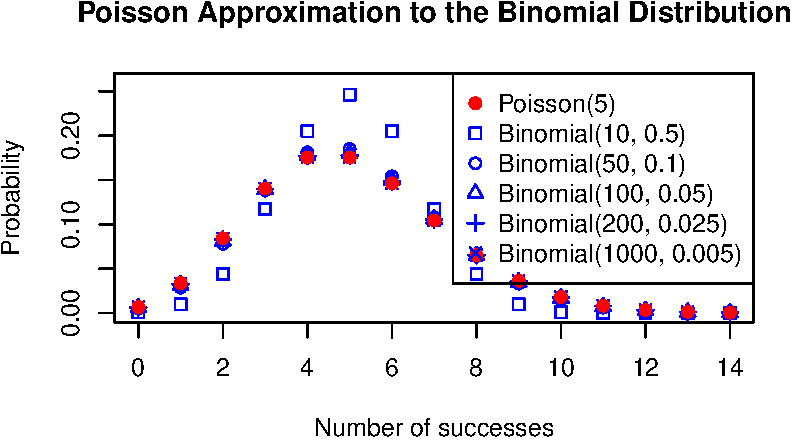
\includegraphics[keepaspectratio]{notes/chapter8_files/figure-pdf/fig-plot-1.pdf}}

}

\end{figure}%

\begin{example}[Charles' Viral Trick-Shot
Attempt]\protect\hypertarget{exm-poi-approx}{}\label{exm-poi-approx}

Charles has been watching online videos of seemingly impossible ``trick
shots'', where individuals toss household objects to land in
increasingly complex locations. Inspired by this trend, Charles decides
to try a version of this at home, where the goal is to bounce a dime off
of the table and have it land in an upright coke bottle. Suppose that
the probability that Charles succeeds on any given attempt of this trick
shot is \(0.01\).

\begin{enumerate}
\def\labelenumi{\alph{enumi}.}
\tightlist
\item
  If Charles attempts the trick shot \(100\) times, what is the
  probability that at least one of the attempts is successful?
\item
  How can the probability in part (a) be approximated using a Poisson?
  How close is the approximation.
\item
  Suppose that Charles instead attempts a new, more challenging the
  trick shot \(1000\) times. This shot has a success probability of just
  \(0.001\). What is the approximate probability that more than one of
  these attempts are successful?
\item
  Do you expect that the probability in (b) or (c) will be closer to the
  truth? Explain.
\end{enumerate}

\begin{tcolorbox}[enhanced jigsaw, arc=.35mm, rightrule=.15mm, breakable, bottomrule=.15mm, left=2mm, toprule=.15mm, leftrule=.75mm, opacityback=0, colback=white, colframe=quarto-callout-color-frame]

\vspace{-3mm}\textbf{Solution}\vspace{3mm}

\begin{enumerate}
\def\labelenumi{\alph{enumi}.}
\tightlist
\item
  The number of successes will follow a \(\text{Bin}(100, 0.01)\). We
  want to know \(P(X \geq 1) = 1 - P(X = 0)\), and so we can compute
  this by calculating
  \[P(X = 0) = \binom{100}{0}(0.01)^{0}(0.99)^{100} = 0.99^{100}.\] As a
  result, the probability of at least one success is \(1 - 0.99^{100}\)
  or approximately 0.634.
\item
  The binomial can be approximated using a
  \(\text{Poi}(100(0.01)) = \text{Poi}(1)\) distribution. In this case,
  \[P(X \geq 1) = 1 - P(X = 0) \approx 1 - \frac{e^{-1}1^0}{0!} = 1 - e^{-1} \approx 0.632.\]
  This approximation differs from the truth by 0.0018471.
\item
  This binomial can be approximated using the same \(\text{Poi}(1)\)
  distribution, since \(1000(0.001) = 1\). As a result, the approximate
  probability will still be \(1 - e^{-1} \approx 0.632\).
\item
  The probability in (c) should be closer to the truth since \(n\) is
  larger and the approximation is based on the limit as \(n\to\infty\).
  Thus, for larger \(n\) with constant \(np\), the approximation should
  improve. Indeed, if we check the actual binomial probability in the
  second case we get 0.6323046 which differs from the approximation by
  just 0.0001840164.
\end{enumerate}

\end{tcolorbox}

\end{example}

\section{Using Named Distributions}\label{using-named-distributions}

While many other named, discrete distributions exist, these are the most
common. When confronted with a problem in the real-world for which you
wish to understand the uncertainty associated with it, a reasonable
first step is to determine whether a named distribution is well-suited
to representing the underlying phenomenon. Is it a situation with
enumerated events which are equally likely? Use the discrete uniform. Is
it a binary outcome? Use the Bernoulli. Are you counting the number of
success in a fixed number of trials? Use the binomial. Are you running
repeated trials until a (certain number of) success(es)? Use the
geometric (or negative binomial). Are you sampling without replacement?
Use the hypergeometric. Are you counting events over a fixed space? Use
the Poisson.

Once identified, the distribution can be used in exactly the same way as
any probability mass function. That is, we still require all the
probability rules, event descriptions, and techniques from before. The
difference in these cases is that we immediately have access to the
correct form of the probability mass function, the expected value, and
the variance.

An additional utility with this approach to solving probability
questions is that, over time and repeated practice, you can build an
intuition as to the behaviour of random variables following these
various distributions. Probabilities in general can be deeply
unintuitive. It can be hard to assess, without formally working it out,
whether an event is likely or unlikely, let alone how likely an event
is. However, the lack of intuition from our wider experience can be
negated almost entirely by building of intuition through the repeated
application of these distributions. You can start to gain a sense of how
binomial random variables behave, being able to determine just from
inspection whether events seem plausible or not. Much of the study of
probability and statistics is about building a set of tools that can
overcome the flaws in our intuitive reasoning regarding uncertainty.
This comes only through practice, however, this framework of named
distributions provides a very solid foundation to perform such practice.

\subsection{Named Distributions in R}\label{named-distributions-in-r}

In R all of the named distributions that we have discussed, and in fact,
many that we have not discussed, are implemented to make calculations
easier. In particular, there are R functions which evaluate the
probability mass function for the various distributions. Alongside
these, there are also functions which calculate what we refer to as the
\emph{cumulative probability}\footnote{More on this in the coming
  chapter.}, which is to say the \(P(X\leq k)\) for some value \(k\).
These functions generally are called \texttt{d\{distname\}}, where
\texttt{\{distname\}} is the name of the relevant distribution. For
instance, \texttt{dbinom} for the binomial, \texttt{dpoi} for the
Poisson, and so forth. These will evaluate the probability mass function
at the relevant values. In order to evaluate the cumulative probability
at the specified values you would call \texttt{p\{distname\}}. These
functions take in a parameter for the value to evaluate at, and then
parameters that correspond to the various parameters from the
distributions themselves.

\begin{Shaded}
\begin{Highlighting}[]
\CommentTok{\# Binomial Distribution}
\FunctionTok{dbinom}\NormalTok{(}\DecValTok{3}\NormalTok{, }\AttributeTok{size =} \DecValTok{10}\NormalTok{, }\AttributeTok{p =} \FloatTok{0.5}\NormalTok{)     }\CommentTok{\# P(X = 3) if X\textasciitilde{}Bin(10, 0.5)}
\FunctionTok{pbinom}\NormalTok{(}\DecValTok{3}\NormalTok{, }\AttributeTok{size =} \DecValTok{10}\NormalTok{, }\AttributeTok{p =} \FloatTok{0.5}\NormalTok{)     }\CommentTok{\# P(X \textless{}= 3)}

\CommentTok{\# Geometric Distribution}
\FunctionTok{dgeom}\NormalTok{(}\DecValTok{10}\NormalTok{, }\AttributeTok{prob =} \FloatTok{0.1}\NormalTok{)             }\CommentTok{\# P(X=10) if X\textasciitilde{}Geo(0.1)}
\FunctionTok{pgeom}\NormalTok{(}\DecValTok{10}\NormalTok{, }\AttributeTok{prob =} \FloatTok{0.1}\NormalTok{)             }\CommentTok{\# P(X\textless{}=10)}

\CommentTok{\# Negative Binomial}
\FunctionTok{dnbinom}\NormalTok{(}\DecValTok{6}\NormalTok{, }\AttributeTok{size =} \DecValTok{3}\NormalTok{, }\AttributeTok{prob =} \FloatTok{0.2}\NormalTok{)  }\CommentTok{\# P(X=6) if X\textasciitilde{}NB(6, 0.2)}
\FunctionTok{pnbinom}\NormalTok{(}\DecValTok{6}\NormalTok{, }\AttributeTok{size =} \DecValTok{3}\NormalTok{, }\AttributeTok{prob =} \FloatTok{0.2}\NormalTok{)  }\CommentTok{\# P(X\textless{}=6)}

\CommentTok{\# Hypergeometric}
\CommentTok{\# In this case, X \textasciitilde{} HG(N=n+m, M = m, n = k)}
\FunctionTok{dhyper}\NormalTok{(}\DecValTok{2}\NormalTok{, }\AttributeTok{m =} \DecValTok{6}\NormalTok{, }\AttributeTok{n =} \DecValTok{9}\NormalTok{, }\AttributeTok{k =} \DecValTok{4}\NormalTok{)    }\CommentTok{\# P(X=2) X \textasciitilde{} HG(15, 6, 4)}
\FunctionTok{phyper}\NormalTok{(}\DecValTok{2}\NormalTok{, }\AttributeTok{m =} \DecValTok{6}\NormalTok{, }\AttributeTok{n =} \DecValTok{9}\NormalTok{, }\AttributeTok{k =} \DecValTok{4}\NormalTok{)    }\CommentTok{\# P(X\textless{}=2)}

\CommentTok{\# Poisson}
\FunctionTok{dpois}\NormalTok{(}\DecValTok{5}\NormalTok{, }\AttributeTok{lambda =} \DecValTok{4}\NormalTok{)              }\CommentTok{\# P(X=5) X \textasciitilde{} Poi(4)}
\FunctionTok{ppois}\NormalTok{(}\DecValTok{5}\NormalTok{, }\AttributeTok{lambda =} \DecValTok{4}\NormalTok{)              }\CommentTok{\# P(X\textless{}=5)}

\DocumentationTok{\#\# [1] 0.1171875}
\DocumentationTok{\#\# [1] 0.171875}
\DocumentationTok{\#\# [1] 0.03486784}
\DocumentationTok{\#\# [1] 0.6861894}
\DocumentationTok{\#\# [1] 0.05872026}
\DocumentationTok{\#\# [1] 0.2618025}
\DocumentationTok{\#\# [1] 0.3956044}
\DocumentationTok{\#\# [1] 0.8571429}
\DocumentationTok{\#\# [1] 0.1562935}
\DocumentationTok{\#\# [1] 0.7851304}
\end{Highlighting}
\end{Shaded}

Note that we have seen the \texttt{sample} function before, which is an
implementation of the discrete uniform. To implement the Bernoulli, we
can use the binomial distribution with \(n=1\). It is a worthwhile
exercise to see if you can use R to start answering the questions from
this chapter, numerically. This is the first prominent use case for R
programming which can save a tremendous amount of time, and is likely
the first use case that becomes directly relevant to the course
material.

\section*{Exercises}\label{exercises-6}
\addcontentsline{toc}{section}{Exercises}

\markright{Exercises}

\begin{exercise}[]\protect\hypertarget{exr-8.1}{}\label{exr-8.1}

For each of the following scenarios, describe which distribution the
indicated random variable most closely resembles, and why.

\begin{enumerate}
\def\labelenumi{\alph{enumi}.}
\tightlist
\item
  In a manufacturing process, you're interested in the number of trials
  required to produce the first defective item.
\item
  A hospital wants to study the number of patients arriving at the
  emergency room in a fixed time interval, where the arrival rate is low
  and the events are rare.
\item
  A quality control team inspects a batch of items and classifies each
  batch as either defective or non-defective.
\item
  In a survey, you want to determine the number of people who prefer
  online shopping over in-store shopping.
\item
  Researchers are studying a group of patients with a very rare disease.
  They wish to know whether a particular gene mutation is associated
  with the disease or not. They sample members of the population who
  have the disease to further study.
\item
  An online streaming platform wants to model the number of times a
  specific video is watched in an hour, given a known average view rate.
\item
  A baseball player wants is interested in the number of home runs they
  hit in a game, where the probability of hitting a home run is the same
  for each at-bat.
\item
  A call center manager wants to model the number of calls received per
  minute during a quiet period of the day.
\item
  In a network setup, multiple backup routers are used, and the network
  remains functional as long as a certain number of them are
  operational. A network engineer is interested in how many backup
  routers are needed to ensure network reliability under various failure
  scenarios.
\end{enumerate}

\end{exercise}

\begin{exercise}[]\protect\hypertarget{exr-8.2}{}\label{exr-8.2}

Show that if \(X\sim\text{Bern}(p)\) then \(E[X] = p\) and
\(\text{var}(X) = p(1-p)\).

\end{exercise}

\begin{exercise}[]\protect\hypertarget{exr-8.3}{}\label{exr-8.3}

Show that if \(X_1,\dots,X_r\stackrel{iid}{\sim}\text{Geo}(p)\) and
\(Y=\sum_{i=1}^r X_i\), then \(Y\) follows a negative binomial
distribution. Find the mean and variance of this distribution, and
indicate which negative binomial distribution it is.

\end{exercise}

\begin{exercise}[]\protect\hypertarget{exr-8.4}{}\label{exr-8.4}

Suppose that \(X\) follows a Binomial distribution with \(8\) trials and
probability of success \(0.4\). Find:

\begin{enumerate}
\def\labelenumi{\alph{enumi}.}
\tightlist
\item
  \(P(X=2)\).
\item
  \(P(X = 4)\).
\item
  \(P(X < 2)\).
\item
  \(P(X > 6)\).
\item
  \(E[X]\).
\item
  \(\text{var}(X)\).\\
\end{enumerate}

\end{exercise}

\begin{exercise}[]\protect\hypertarget{exr-8.5}{}\label{exr-8.5}

If \(20\%\) of bolts produced by a machine are defective, determine the
probability that out of \(4\) bolts chosen at random:

\begin{enumerate}
\def\labelenumi{\alph{enumi}.}
\tightlist
\item
  \(1\) is defective.
\item
  \(0\) are defective.
\item
  fewer than \(2\) bolts are defective.
\end{enumerate}

\end{exercise}

\begin{exercise}[]\protect\hypertarget{exr-8.6}{}\label{exr-8.6}

Of all the weld failures in a certain assembly, \(85\%\) of them occur
in the weld metal itself, and the remaining \(15\%\) occur in the base
metal. A sample of \(20\) weld failures is examined.

\begin{enumerate}
\def\labelenumi{\alph{enumi}.}
\tightlist
\item
  What is the probability that exactly five of them are base metal
  failures?
\item
  What is the probability that fewer than four of them are base metal
  failures?
\item
  What is the probability that none of them are base metal failures?
\end{enumerate}

\end{exercise}

\begin{exercise}[]\protect\hypertarget{exr-8.7}{}\label{exr-8.7}

Celeste and Dana are playing squash, and Dana is determined to win at
least two games. Unfortunately, his chance of winning any one game is
only \(\frac{1}{4}\), and this chance remains constant however many
games he plays against Celeste. The players agree to play \(5\) games
and, if Dana has won at least two by then, play ceases. Otherwise, Dana
persuades Celeste to play a further \(5\) games with him. What is the
probability that a. only \(5\) games are played, and Dana wins at least
two of them; a. that \(10\) games are played, and Dana wins at least two
of them.

\end{exercise}

\begin{exercise}[]\protect\hypertarget{exr-8.8}{}\label{exr-8.8}

A machine produces bolts, and for each bolt there is a probability \(p\)
of it being defective, where results for different bolts are assumed
independent. A large batch of the machine's production is inspected by a
customer in order to determine whether the batch should be purchased. In
the inspection, \(10\) bolts are selected at random and examined: if
none is defective the batch is accepted, and if three or more is
defective, the batch is rejected. If only \(1\) or \(2\) are defective,
a further batch of \(10\) is selected. If in total between the two
batches three or more are defective, the batch is rejected.

\begin{enumerate}
\def\labelenumi{\alph{enumi}.}
\tightlist
\item
  What is the probability that a decision is made at the first stage?
\item
  What is the probability that the batch is accepted if \(p=0.15\).
\end{enumerate}

\end{exercise}

\begin{exercise}[]\protect\hypertarget{exr-8.9}{}\label{exr-8.9}

Find the probability of getting a total of \(7\) at least once in three
tosses of a pair of fair dice.

\end{exercise}

\begin{exercise}[]\protect\hypertarget{exr-8.10}{}\label{exr-8.10}

Twenty air-conditioning units have been brought in for service. Twelve
of the units have broken compressors and the other eight have broken
fans. If seven of these units are randomly selected for repair, what is
probability that exactly three have broken fans?

\end{exercise}

\begin{exercise}[]\protect\hypertarget{exr-8.11}{}\label{exr-8.11}

The probability that a computer running a certain operating system
crashes on any given day is \(0.1\).

\begin{enumerate}
\def\labelenumi{\alph{enumi}.}
\tightlist
\item
  Find the probability that the computer crashes for the first time on
  the twelfth day.
\item
  Find the probability that the third crash comes on day \(30\).
\end{enumerate}

\end{exercise}

\begin{exercise}[]\protect\hypertarget{exr-8.12}{}\label{exr-8.12}

There are \(30\) restaurants in a particular town. If you assume that
\(4\) of them have health code violations, and a health inspector is
going to visit \(10\) of them at random, what is the probability that:

\begin{enumerate}
\def\labelenumi{\alph{enumi}.}
\tightlist
\item
  Exactly two of the restaurants visited will have violations.
\item
  None of the restaurants visited will have violations?
\end{enumerate}

\end{exercise}

\begin{exercise}[]\protect\hypertarget{exr-8.13}{}\label{exr-8.13}

A traffic light at a certain intersection is green \(0.5\) of the time,
yellow \(0.1\) of the time, and red the remainder of the time. A car
approaches the intersection once per day, at a random time. Suppose that
\(X\) represents the number of days until the car reaches three red
lights.

\begin{enumerate}
\def\labelenumi{\alph{enumi}.}
\tightlist
\item
  Find \(P(X = 7)\).
\item
  What is \(E[X]\).
\item
  Suppose that the car only drives on weekdays, and the first day under
  consideration is a Saturday. What is \(P(X \leq 18)\)?
\end{enumerate}

\end{exercise}

\begin{exercise}[]\protect\hypertarget{exr-8.14}{}\label{exr-8.14}

A computer program has a bug that causes it to fail in one out of every
thousand runs, on average. In order to find the bug the program is run,
independently, until it has failed \(5\) times.

\begin{enumerate}
\def\labelenumi{\alph{enumi}.}
\tightlist
\item
  How many times will the program need to run, on average?
\item
  If it takes \(30\) seconds to run the program, what is the standard
  deviation for the amount of time that this debugging will take?
\end{enumerate}

\end{exercise}

\begin{exercise}[]\protect\hypertarget{exr-8.15}{}\label{exr-8.15}

Ten items are to be sampled from a lot of \(60\). If more than one is
defective, the lot will be rejected. What is the probability that the
lot will be rejected if:

\begin{enumerate}
\def\labelenumi{\alph{enumi}.}
\tightlist
\item
  there are \(5\) defective items.
\item
  there are \(10\) defective items.
\item
  there are \(20\) defective items.
\end{enumerate}

\end{exercise}

\begin{exercise}[]\protect\hypertarget{exr-8.16}{}\label{exr-8.16}

Suppose that \(X\) is a Poisson random variable with rate \(4\). Find

\begin{enumerate}
\def\labelenumi{\alph{enumi}.}
\tightlist
\item
  \(P(X=1)\)
\item
  \(P(X=0)\)
\item
  \(P(X < 2)\)
\item
  \(P(X > 1)\)
\item
  \(E[X]\)
\item
  \(\text{var}(X)\).
\end{enumerate}

\end{exercise}

\begin{exercise}[]\protect\hypertarget{exr-8.17}{}\label{exr-8.17}

The number of flaws in a given area of aluminum foil happen uniformly at
a rate of \(3\) per square metre. If \(X\) represents the number of
flaws in a \(1m^2\) random sample of foil, what is

\begin{enumerate}
\def\labelenumi{\alph{enumi}.}
\tightlist
\item
  \(P(X=5)\).
\item
  \(P(X = 0)\).
\item
  \(P(X < 2)\).
\item
  \(P(X > 1)\).
\end{enumerate}

\end{exercise}

\begin{exercise}[]\protect\hypertarget{exr-8.18}{}\label{exr-8.18}

Negative reactions from a particular injection occur at a rate of \(1\)
per \(1000\) people in the population. Suppose that \(2000\) people
receive the injection.

\begin{enumerate}
\def\labelenumi{\alph{enumi}.}
\tightlist
\item
  What is the probability that exactly \(3\) individuals have a negative
  reaction?
\item
  What is the probability that more than \(2\) individuals have a
  negative reaction?
\end{enumerate}

\end{exercise}

\begin{exercise}[]\protect\hypertarget{exr-8.19}{}\label{exr-8.19}

A telephone exchange receives, on average, \(5\) calls per minute. Find
the probability that

\begin{enumerate}
\def\labelenumi{\alph{enumi}.}
\tightlist
\item
  in a \(1\) minute period, no calls are received.
\item
  in a \(2\) minute period, fewer than \(4\) calls are received.
\item
  in \(5\) separate \(1\) minute periods there are exactly four in which
  \(2\) or more calls are received.
\end{enumerate}

\end{exercise}

\begin{exercise}[]\protect\hypertarget{exr-8.20}{}\label{exr-8.20}

The number of defective components produced in a process follows a
Poisson distribution with a mean of \(20\). Every defective item has a
probability of \(0.6\) of being repaired, independently of all others.

\begin{enumerate}
\def\labelenumi{\alph{enumi}.}
\tightlist
\item
  Find the probability that exactly \(15\) defective components are
  produced.
\item
  Given that exactly \(15\) defective components are produced, find the
  probability that exactly \(10\) can be repaired.
\item
  If \(N\) is the number of components produced, and \(X\) is the number
  which are repairable, then given the value of \(N\), what is the pmf
  of \(X\)?
\end{enumerate}

\end{exercise}

\begin{exercise}[]\protect\hypertarget{exr-8.21}{}\label{exr-8.21}

Suppose that \(X \sim \text{Bin}(200, 0.04)\).

\begin{enumerate}
\def\labelenumi{\alph{enumi}.}
\tightlist
\item
  What is the approximate probability that \(X = 4\)?
\item
  Is your answer from (a) likely to be closer or further from the truth
  compared to if \(X\) followed a \(\text{Bin}(2000, 0.004)\)
  distribution? Explain.
\end{enumerate}

\end{exercise}

\begin{exercise}[]\protect\hypertarget{exr-8.22}{}\label{exr-8.22}

Suppose that a company manufactures components in lots. Their contracts
stipulate that in lots of \(200\), no more than \(4\) components can be
defective. If there are more than \(4\) defective components, the lot is
rejected. If each manufactured component has a probability of being
defective of \(0.01\), what is the approximate probability that the lot
is rejected?

\end{exercise}

\begin{exercise}[]\protect\hypertarget{exr-8.23}{}\label{exr-8.23}

The Poisson distribution has the property that, for
\(X\sim\text{Poi}(\lambda)\), \(E[X] = \text{var}(X)\). We also know
that the limiting distribution of a \(\text{Bin}(n, p)\) distribution is
a Poisson. Explain how these two facts can be reconciled with one
another.

\end{exercise}

\begin{exercise}[]\protect\hypertarget{exr-8.24}{}\label{exr-8.24}

Suppose that a popular website is analyzing their traffic to determine
the stability of their servers. Their analysis concludes that, on
average, \(3\) users per hour face a server issue preventing them from
accessing the service.

\begin{enumerate}
\def\labelenumi{\alph{enumi}.}
\tightlist
\item
  If, in in one particular hour, there are \(10,000\) visitors, what
  distribution best models the number of users who face server issues?
\item
  Suppose that the company is concerned with the number of individuals
  who cannot access the website over a \(2\) hour period, without
  knowing precisely how many visitors they receive during that time.
  Approximate the probability that they will have more than \(4\)
  visitors not being able to access the site, and explain why this is a
  reasonable approximation.
\end{enumerate}

\end{exercise}

\chapter{Continuous Random Variables}\label{sec-continuous-rv}

Our discussions of probability distributions and their summaries have
focused entirely on discrete random variables. To recap, a discrete
random variable is any random numeric quantity that can take on a
countable number of values. Discrete random variables are defined in
contrast to continuous random variables, which take on values over the
span of intervals in uncountably large sets. Suppose that \(X\) can take
any real number between \(0\) and \(1\). There is no way to enumerate
the set of possible values for this random quantity, and so it must not
be discrete.

Many quantities of interest are better treated as a continuous quantity
rather than a discrete one even when this is not technically correct.
For instance, time measured in seconds is often best thought of as
continuous, even though any stop watch used to grab these measurements
will have some limit to the precision with which they can measure.
Similarly, lengths and heights will often be better treated as
continuous quantities, even though any measuring device will necessarily
have some minimal threshold after which it cannot discern distances.
Thus, deciding whether a quantity is continuous or discrete is sometimes
a judgment call. In general discrete quantities are harder to work with
when the set of possibilities is very large. In these cases, not much is
lost by treating the random variables as though they were continuous.
This distinction is another area which requires the active development
of intuition, but once present, the distinctions become second
nature.\footnote{Recall Example~\ref{exm-discrete-vs-continuous-rv} for
  practice in this.}

\section{Continuous Versus Discrete}\label{continuous-versus-discrete}

Distinguishing whether a random quantity is continuous or discrete is
crucial as, broadly speaking, the two types of quantities are treated
differently. The same underlying ideas are present, but the distinctions
between the two settings require some careful thought. The use of
continuous random variables necessitates an understanding of
introductory calculus. These course notes are designed to be understood
without any experience in calculus, and as a result, we will first
present continuous random variables in general, without the need for
calculus. Additional sections containing the technical details follow.
Despite requiring calculus to be complete understood, continuous random
variables are \emph{the} dominant type of random variables outside of
introductory courses. As a result, understanding the distinctions, and
becoming familiar with how they are to be manipulated is an important
skill.

The key difference between discrete and continuous random variables is
that, for discrete random variables the behaviour is governed by
assessing \(P(X=x)\) for all possible values of \(x\), while for
continuous random variables \(P(X=x)=0\) for \textbf{every} value of
\(x\). This is likely a surprising statement, and as such it is worth
reiterating. With discrete random variables we discussed how all of the
probabilistic behaviour is governed by the probability mass function.
This is defined as \(p_X(x) = P(X=x)\). If \(X\) is a continuous random
variable, we must have \(P(X=x) = 0\). Correspondingly, continuous
random variables do not have probability mass functions, and to
understand the behaviour of these random variables we must us other
quantities.

\begin{tcolorbox}[enhanced jigsaw, arc=.35mm, title={Singleton Probabilities with Continuous Random Variables}, rightrule=.15mm, coltitle=black, opacitybacktitle=0.6, colbacktitle=quarto-callout-note-color!10!white, leftrule=.75mm, colback=white, breakable, titlerule=0mm, toptitle=1mm, bottomtitle=1mm, bottomrule=.15mm, toprule=.15mm, opacityback=0, left=2mm, colframe=quarto-callout-note-color-frame]

While the fact that \(P(X=x) = 0\) may seem unintuitive at first glance,
it is worth exploring this even further. The nature of a continuous
random variable is such that there is no possible way to enumerate all
of the values that are possible to be realized by the random quantity.
Suppose that we take a set of countably many possible observations and
gave each of these a probability of greater than \(0\) of occurring.
Even if we take an infinite number of them, there will still be an
uncountably infinite number of events in the sample space that we have
not accounted for. We know that the total probability of the sample
space must be \(1\), and so we must have the total probability of the
first set of events being less than \(1\)\footnotemark{}.

Now suppose we take another set of countably many events, again giving
each of them a positive probability. Once more the sum of all of these
probabilities must be less than \(1\), and specifically, the sum of both
sets must also be less than \(1\). Even after these two sets, there are
still uncountably infinite events to go and so we continue this process.
Because we always need the total probability to be \(1\) once all events
have been accounted for, and because we will always have uncountably
infinite events remaining to account for, we can \textbf{never} have a
positive probability assigned to each event in a set of events. Even if
we made the probability of each of these sets very, very
small\footnotemark{} after some fixed number of countable events the
probabilities would be greater than \(1\), which cannot happen. As such,
each event itself must have \(0\) probability.

An alternative technique for understanding this intuition is to think
about how unlikely it really would be to observe any specific value.
Suppose that \(X\) takes values on the interval \([0,1]\). Recall that,
when we defined probabilities, we discussed them as being the long run
proportion of time that an event occurs. Take some event, say \(X=0.5\).
Suppose that we took repeated measurements of \(X\) which are
independent and identically distributed. Now suppose that at some point
we exactly do observe \(X=0.5\). Should we expect that this will ever
happen again? The next time we get near \(0.5\), might we instead
observe \(0.51\) or \(0.49\) or \(0.5000000000000000001\) or any of the
other uncountably infinite values in the very near vicinity of \(0.5\)?
Each time that we make an observation the denominator of our proportion
is growing, but if every value between \(0\) and \(1\) is truly
possible, as time goes on the number of times that \(X=0.5\) must stay
much, much smaller than the total number of trials. If we continue this
off to infinity, in the limit, the probability must become \(0\).

This conclusion leads to a few different points. First, impossibility is
not the same as probability \(0\). Impossible events do have probability
\(0\), but possible events may also have probability \(0\). Events which
are outside of the sample space are impossible. Events inside the sample
space, even probability zero events, remain possible. Second, we require
alternative mathematical tools for discussing the probability of events
in a continuous setting. Ideally this would be analogous to a
probability mass function, but would somehow function in the case of
continuity.

\end{tcolorbox}

\footnotetext{If it summed to \(1\) then this would not be a continuous
random variable, since there would only be a countable number of
possible events.}

\footnotetext{Like, \(1\) in a million, or \(1\) in a billion, or \(1\)
in the number of atoms in the universe.}

\section{Cumulative Distribution
Functions}\label{cumulative-distribution-functions}

To begin building to the continuous analogue of the probability mass
function, we will start by focusing on events that are easier to define
in the continuous case. Suppose that \(X\) is defined on some continuous
interval. Instead of thinking of events relating to \(X=x\), we instead
turn our focus to events of the form \(X \in (a,b)\) for some interval
defined by the endpoints \(a\) and \(b\). Now note that, relying only on
our knowledge of probabilities relating to generic events, we can
rewrite \(P(X\in(a,b))\) slightly. Specifically, \begin{align*}
P(X\in(a,b)) &= 1 - P(X\not\in(a,b))\\
&= 1 - P(\{X < a\}\cup\{X > b\}) \\
&= 1 - \left(P(X < a) + P(X > b)\right)\\
&= 1 - P(X > b) - P(X < a)\\
&= P(X < b) - P(X < a).\end{align*}

\begin{figure}[H]

\caption{\label{fig-number-line}A number line showcasing the interval
\((a,b)\) and demonstrating how you can take everything less than \(b\)
and remove all that is less than \(a\) to be left with only \((a,b)\).}

\centering{

\pandocbounded{\includegraphics[keepaspectratio]{graphics/ch9-difference-in-numbers.png}}

}

\end{figure}%

In words we know that the probability that \(X\) falls into any
particular interval is given by the probability that it is less than the
upper bound of the interval minus the probability that it is less than
the lower bound of the interval. Notice that \(X < a\) is an event, and
if we knew how to assign probabilities to \(X<a\) for arbitrary \(a\),
then we could assign probabilities to any interval. Also note that, even
in the continuous case, it make sense to talk of \(P(X < a)\) for some
value \(a\). These intervals will contain an uncountably infinite number
of events, and as such, can certainly occur with greater than \(0\)
probability.

Consider an example with \(X\) defined on \([0,1]\). In this case we
know that \(P(X<1)=1\). Note that we could have written
\(P(X \leq 1) = 1\), which may have been more obviously true. However,
\(P(X\leq 1) = P(\{X<1\}\cup\{X=1\}) = P(X<1) + P(X=1)\) and we know
that \(P(X=1)=0\). In the continuous case we do not need to worry
whether we use \(X\leq a\) or \(X < a\), and we will interchange them
throughout.

\begin{example}[Charles and Sadie Wait for the
Bus]\protect\hypertarget{exm-charles-and-sadie-bus-times}{}\label{exm-charles-and-sadie-bus-times}

Charles and Sadie are visiting a large city and are getting around via
public transit while there. They are not quite familiar with the bus
schedules yet, but they know that the bus they are waiting for will show
up sometime in the next \(15\) minutes. They realize that this is a
continuous random quantity, and decide to pass the time by trying to
reason about how long they will be waiting for the bus to arrive. To do
so, they make the assumption that the bus is equally likely to show at
any point during this interval.

\begin{enumerate}
\def\labelenumi{\alph{enumi}.}
\tightlist
\item
  What is the probability that Charles and Sadie wait \(15\) or fewer
  minutes for the bus?
\item
  What is the probability that Charles and Sadie wait \(5\) or fewer
  minutes for the bus?
\item
  What is the probability that Charles and Sadie wait exactly \(7\)
  minutes for the bus?
\item
  What is the probability that Charles and Sadie wait between \(8\) and
  \(12\) minutes for the bus?
\item
  What is the probability that Charles and Sadie have to wait longer
  than \(13\) minutes for the bus?
\end{enumerate}

\begin{tcolorbox}[enhanced jigsaw, arc=.35mm, rightrule=.15mm, breakable, bottomrule=.15mm, left=2mm, toprule=.15mm, leftrule=.75mm, opacityback=0, colback=white, colframe=quarto-callout-color-frame]

\vspace{-3mm}\textbf{Solution}\vspace{3mm}

Let \(X\) represent the amount of time that they wait for the bus.

\begin{enumerate}
\def\labelenumi{\alph{enumi}.}
\tightlist
\item
  If we trust their judgment, then they have claimed that they will wait
  between \(0\) and \(15\) minutes for the bus. As a result,
  \(P(X \leq 15) = 1\).
\item
  Here we can reason that if any time is equally likely for the bus to
  arrive, then the first \(5\) minutes must be as likely as the second
  interval of \(5\) minutes or the third. That is, in the first \(5\)
  minutes there is a total of \(\dfrac{5}{15} = \dfrac{1}{3}\) of the
  possible arrival times taken up, and so we must conclude that
  \(P(X \leq 5) = \dfrac{1}{3}\).
\item
  This would be \(P(X = 7)\). \(X\) is a continuous quantity, and so
  \(P(X = 7) = 0\).
\item
  We can reason through this in two different ways. First, we can use
  the property discussed above that
  \(P(X \in (8, 12)) = P(X \leq 12) - P(X\leq 8)\), and then use the
  same procedure as in (b). That gives
  \[P(X \in (8, 12)) = \dfrac{12}{15} - \dfrac{8}{15} = \dfrac{4}{15}.\]
  Alternatively, because each interval of the same length must be
  equally likely, we can reason that this is just a length \(4\)
  interval. Thus, it must have the same likelihood as any other length
  \(4\) interval, given by \(\dfrac{4}{15}\).
\item
  Note that, longer than \(13\) is the complement to less than \(13\).
  Thus,
  \[P(X \geq 13) = 1 - P(X \leq 13) = 1 - \dfrac{13}{15} = \dfrac{2}{15}.\]
\end{enumerate}

\end{tcolorbox}

\end{example}

The centrality of events of the form \(X \leq a\) prompts further
consideration the \textbf{cumulative distribution function} (introduced
in Definition~\ref{def-cumulative-distribution-function}).

\begin{definition}[Cumulative Distribution
Function]\protect\hypertarget{def-cumulative-distribution-function}{}\label{def-cumulative-distribution-function}

The cumulative distribution function of a random variable \(X\),
typically denoted as \(F(x)\) or \(F_X(x)\), is defined as the function
that gives the probability that the random variable is less than or
equal to some threshold.

That is, \(F_X(x) = P(X \leq x)\). We may also refer to the cumulative
distribution function simply as the \textbf{distribution function}.

\end{definition}

Once we have defined the distribution function for a random variable,
using the above derivation we are able to determine the probability
associated with any events based on intervals. The cumulative
distribution function for continuous random variables is central to
nearly every probability calculation that is performed. In the discrete
case, since it is simply the summation of the probability mass function,
it tends to be a less useful quantity.

Suppose that, for a random variable \(X\), we know the cumulative
distribution function. This knowledge permits the computation of
\emph{any} probability associated with the random variable. Consider
some event defined in terms of \(X\) which we may wish to determine the
probability of. We know that events are subsets of the sample space.
Every one of these events can be written using our basic set operations
(unions, intersections, and complements) applied to intervals of the
form \((a,b)\) and sets of the form \(\{x\}\).\footnote{These are called
  singletons. We addressed these in terms of probability assignment
  using the language of singletons above. As a general rule, when
  working with continuous quantities, we simply ignore all of the
  singletons.} The axioms of probability allow us to compute
probabilities across the set operations. Further, our knowledge of the
cumulative distribution function, the conversion of \(P(X \in (a,b))\)
into \(F_X(b) - F_X(a)\), and the fact that \(P(X=x) = 0\) for all \(x\)
gives all of the results we need to derive probabilities for these
events.

\begin{example}[Charles and Sadie's Light
Bulbs]\protect\hypertarget{exm-lightbulb-cumulative-distribution-function}{}\label{exm-lightbulb-cumulative-distribution-function}

Charles and Sadie decide that they need to replace some light bulbs. In
their research online, a particular manufacturer of light bulbs,
\emph{Bayesian Brights}, lists the cumulative distribution function for
the lifetime of their bulbs, in hours. The model Charles and Sadie are
considering is said to have a lifetime (in hours) governed by
\[F_X(x) = 1 - \exp\left(-\frac{x}{10000}\right).\]

\begin{enumerate}
\def\labelenumi{\alph{enumi}.}
\tightlist
\item
  What is the probability that a purchased lightbulb lasts for less than
  \(5000\) hours?
\item
  What is the probability that a purchased lightbulb lasts for between
  \(7500\) and \(12000\) hours?
\item
  What is the probability that a purchased lightbulb lasts for more than
  \(8000\) hours?
\end{enumerate}

\begin{tcolorbox}[enhanced jigsaw, arc=.35mm, rightrule=.15mm, breakable, bottomrule=.15mm, left=2mm, toprule=.15mm, leftrule=.75mm, opacityback=0, colback=white, colframe=quarto-callout-color-frame]

\vspace{-3mm}\textbf{Solution}\vspace{3mm}

\begin{enumerate}
\def\labelenumi{\alph{enumi}.}
\tightlist
\item
  Using the given cumulative distribution function this can be
  calculated as
  \[P(X \leq 5000) = F(5000) = 1 - \exp\left(-\frac{5000}{10000}\right) = 1 - e^{-1/2} \approx 0.39346934.\]
\item
  Here we get
  \begin{multline*}P(X \in (7500,12000)) = P(X \leq 12000) - P(X\leq 7500) = F(12000) - F(7500) \\
  = \exp\left(-0.75\right) - \exp\left(-1.2\right) \approx 0.171172341.\end{multline*}
\item
  We can convert this to be the complement event so that it is
  expressible in terms of the cumulative distribution function. That is,
  \(P(X \geq 8000) = 1 - P(X \leq 8000)\), and so
  \[P(X \geq 8000) = 1 - F(8000) = 1 - (1 - e^{-0.8}) = e^{-0.8} \approx 0.449328964.\]
\end{enumerate}

\end{tcolorbox}

\end{example}

\section{The Probability Density
Function}\label{the-probability-density-function}

The distribution function will be the core object used to discuss the
probabilistic behaviour of a continuous random variable. All of the
behaviour of these random quantities will be described by the
distribution function, and as such we will take the distribution
function as a function which defines the distribution of a continuous
random quantity. This is all that we need in order to analyze these
random variables, however, it may be a little unsatisfying in contrast
with the discrete case.

We had set out to find a quantity that paralleled the probability mass
function. Instead, we concluded that the cumulative distribution
function can be made to play the same role in terms of describing the
behaviour of the random quantity. Still, it may be of interest for us to
have a function which takes into account the \emph{relative likelihood}
of being near some value. Suppose, for instance, that for a random
variable defined on \([0,1]\) we wanted to know how likely it was to be
in the vicinity of \(X=0.5\). We could take a small number, say
\(\delta = 0.01\) and calculate
\[P(X\in(0.5-\delta,0.5+\delta)) = F(0.5+\delta)-F(0.5-\delta).\] This
is perfectly well defined based on our discussions to this point. Now,
suppose that \(\delta\) is small enough so that it is reasonable to
assume that this probability is fairly evenly distributed throughout the
interval. Then, if we wanted to assign a likelihood to each value, we
could divide this total probability by the length of the interval,
\(2\delta\). As a result, in this case, the probability that \(X\) is
nearly \(0.5\) will be approximately given by the expression
\[\dfrac{F(0.5+\delta)-F(0.5-\delta)}{2\delta}.\]

We had taken \(\delta=0.01\), but the same process could be applied for
smaller and smaller \(\delta\), say \(0.001\) or \(0.0001\).
Intuitively, as the size of this interval shrinks more and more we are
getting a better and better estimate for the likelihood that the random
variable is in the immediate vicinity of \(0.5\). Moreover, as
\(\delta\) gets smaller and smaller our assumption of a uniform
probability over the interval becomes more and more reasonable.
Unfortunately, we cannot set \(\delta=0\), exactly. We can ask what
happens \emph{in the limit} as \(\delta\) continues to get smaller and
smaller. This question is in the purview of calculus, and can in fact be
answered. While working out the answer is beyond the scope of the
course, we will provide the result anyway.\footnote{If you have taken
  calculus, you may recognize this process as feeling related to the
  first principle definition of a derivative. While it is often
  described in a slightly different way, this feeling of connection is
  intentional.} The resulting function is called the \textbf{probability
density function}, and is related to the cumulative distribution
function through derivatives (and integrals).

\begin{definition}[Probability Density
Function]\protect\hypertarget{def-probability-density-function}{}\label{def-probability-density-function}

A random variable \(X\), with cumulative distribution function \(F(x)\),
is further characterized by its probability density function, denoted
\(f(x)\). The density function describes the relative likelihood of a
random variable taking on values in a particular interval, and mirrors
the behaviour of the probability mass function in the discrete case.
Formally, the probability density function is equal to the derivative of
the cumulative distribution function.

\end{definition}

Roughly speaking, the density function evaluates how likely it is for a
continuous quantity to be in a small neighbourhood of the given value.
Critically, \textbf{probability density functions do not give
probabilities directly}. In fact, probability density functions may give
values that are greater than \(1\)!\footnote{This is not a rare
  occurrence either. For instance, if we consider a random variable that
  will take on values in the interval \([0,0.5]\) with equal likelihood,
  the probability density function in this case will be \(f(x) = 2\).}
Still, if we see the shape of the probability density function, we can
state how likely it is to make observations near the results of
interest. We will often graph the density functions. The high points of
the graph indicate regions with more probability than the regions of the
graph which are lower. Again, the specific probability of any event
\(X=x\) will always be \(0\), but some events fall in neighbourhoods
which are more likely to observe than others.\footnote{Think about the
  fact that, while we may think of human adult heights as a continuous
  quantity, it is far more likely to observe a height around \(5\) feet
  \(6\) inches than around \(9\) feet \(2\) inches.}

\begin{example}[The Types of Busses in the
City]\protect\hypertarget{exm-bus-trips-two}{}\label{exm-bus-trips-two}

After returning from their trip to the big city, Charles and Sadie are
talking to their friend Garth, with a lot more experience in the matter.
Garth explains that there are actually several different types of
busses, with different arrival schedules over the \(15\) minute
interval. Knowing that Charles and Sadie have started to learn about
probability density functions, Garth draws out the following sketch,
giving the probability density function for three different busses.

\pandocbounded{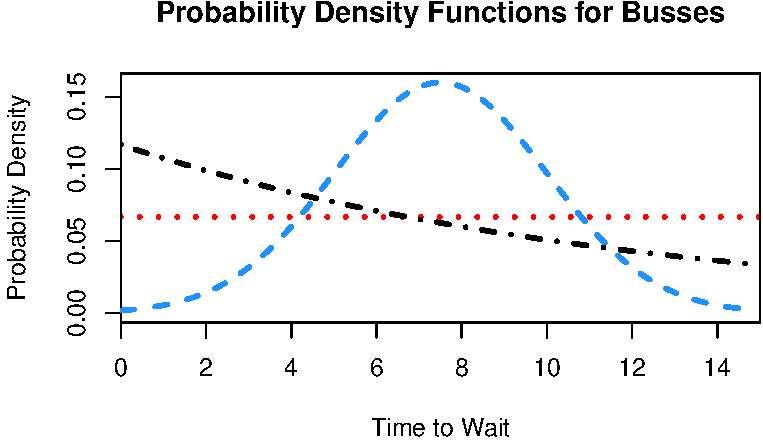
\includegraphics[keepaspectratio]{notes/chapter9_files/figure-pdf/unnamed-chunk-1-1.pdf}}

\begin{enumerate}
\def\labelenumi{\alph{enumi}.}
\tightlist
\item
  Which of the three buses is most likely to show up around the \(1\)
  minute mark?
\item
  Which of the three buses is most likely to show up around the \(6\)
  minute mark?
\item
  Which of the three buses is most likely to show up around the \(14\)
  minute mark?
\item
  Which bus is most likely to show up at \(10\) minutes exactly?
\item
  During which intervals would each of the buses be more likely than the
  other two to arrive?
\item
  Describe the behaviour of each of the three buses.
\end{enumerate}

\begin{tcolorbox}[enhanced jigsaw, arc=.35mm, rightrule=.15mm, breakable, bottomrule=.15mm, left=2mm, toprule=.15mm, leftrule=.75mm, opacityback=0, colback=white, colframe=quarto-callout-color-frame]

\vspace{-3mm}\textbf{Solution}\vspace{3mm}

\begin{enumerate}
\def\labelenumi{\alph{enumi}.}
\tightlist
\item
  At \(x = 1\), the black density is higher than the red density which
  is higher than the blue density. This gives the relative ranking that
  arrivals around \(1\) minute or more likely for the black bus than red
  or blue.
\item
  At \(x = 6\), the blue density is higher than the red or black
  densities, which are roughly the same, and as such, it is the most
  likely bus to arrive in the vicinity of \(6\) minutes.
\item
  At \(14\), the red density is higher than the black density which is
  higher than the blue. This gives the relative ordering of likelihood
  of arrivals.
\item
  All buses have probability \(0\) of arriving at \(10\) minutes exactly
  since these are the densities for continuous random variables.
\item
  The black bus is most likely to arrive for times up until around \(4\)
  minutes, where the blue bus is then the most likely to arrive until
  around \(11\) minutes, where the red bus is most likely to arrive
  until the \(15\) minute mark.
\item
  The red bus has an equal probability of arriving across the full
  interval. The black bus is more likely to arrive near the start of the
  interval, slowly decaying in likelihood as time goes on, while
  remaining fairly likely at the \(15\) minute mark. The blue bus is
  very unlikely to take a very short period of time, or a very long
  period of time, and far more likely to sit in the middle of the
  possible interval.
\end{enumerate}

\end{tcolorbox}

\end{example}

Formally, the probability of any event of interest, say
\(P(X \in [a,b])\) for some interval \([a,b]\), is given by the area
under the probability density function. As a result, if the probability
density function is plotted, then considering the area that is
encompassed within any particular interval (or set of intervals) is
equivalent to considering the probability that the random variable takes
on a value in that range. This can be particularly useful when working
with distributions and trying to get a sense of probabilities: drawing
out the density function, and then highlighting the area of interest is
an effective tool for understanding the probabilities that you are
dealing with.

\begin{example}[Non-Uniform Bus
Arrivals]\protect\hypertarget{exm-area-under-curve}{}\label{exm-area-under-curve}

After some further investigation, Charles and Sadie decide that the
uniformly arriving buses are not actually uniformly arriving. Instead,
there is a lower probability of arriving, which increases for the first
two minutes, then a uniform probability for the next eleven minutes,
followed by a decreasing probability for the final two minutes. Charles
draws a rough sketch of the density function that is expected.

\pandocbounded{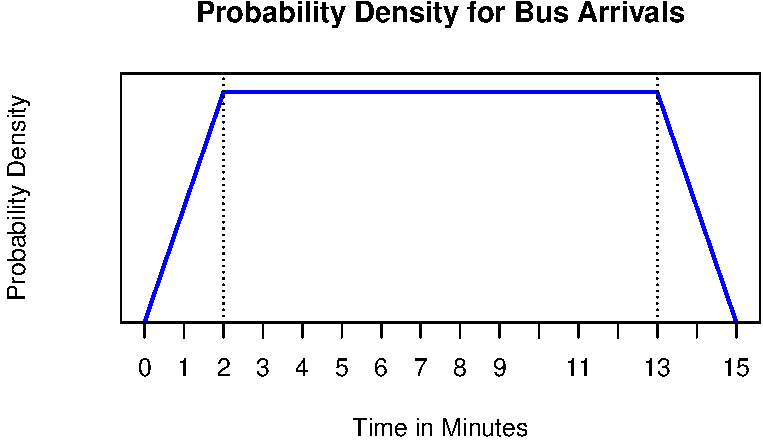
\includegraphics[keepaspectratio]{notes/chapter9_files/figure-pdf/unnamed-chunk-2-1.pdf}}

\begin{enumerate}
\def\labelenumi{\alph{enumi}.}
\tightlist
\item
  At what value is the uniform portion of the probability density
  function depicted?
\item
  What is the probability that the bus arrives in the first two minutes?
\item
  What is the probability that the bus arrives in the final four
  minutes?
\end{enumerate}

\begin{tcolorbox}[enhanced jigsaw, arc=.35mm, rightrule=.15mm, breakable, bottomrule=.15mm, left=2mm, toprule=.15mm, leftrule=.75mm, opacityback=0, colback=white, colframe=quarto-callout-color-frame]

\vspace{-3mm}\textbf{Solution}\vspace{3mm}

\begin{enumerate}
\def\labelenumi{\alph{enumi}.}
\item
  We know that the total probability must equal \(1\). Moreover, we know
  that the probability is given by the area under the curve. This area
  can be decomposed into two triangles, each with a base of \(2\) and an
  unknown height, \(h\), as well as a rectangle with a width of \(11\)
  and a height of \(h\). Thus, using geometric area formulae we get
  \[1 = 2\times\frac{1}{2}\times2\times h + 11\times h = 13h \implies h = \frac{1}{13}.\]
  Thus, the height will be \(\dfrac{1}{13}\).
\item
  The probability that the bus arrives in the first two minutes is the
  area under the curve between \(x = 0\) and \(x = 2\). This is given by
  a triangle with base \(2\) and height (from (a)) of \(\dfrac{1}{13}\).
  Thus, the probability that the bus arrives in the first two minutes is
  \(\dfrac{1}{2}\times2\times\dfrac{1}{13} = \dfrac{1}{13}\).
\item
  The probability that the bus arrives in the final four minutes is the
  same as the area under the curve between \(x=11\) and \(x=15\). This
  can either be computed as a trapezoidal area, or as the area of a
  rectangle plus that of a triangle. The triangle is equivalent to that
  computed for part (b), and the rectangle has a base of \(2\) and a
  height of \(\dfrac{1}{13}\), so that total the area is
  \[2\times\dfrac{1}{13} + \frac{1}{13} = \frac{3}{13}.\]
\end{enumerate}

\end{tcolorbox}

\end{example}

\subsection{\texorpdfstring{\(\int\) The Formal Mathematics for
Continuous Random
Variables}{\textbackslash int The Formal Mathematics for Continuous Random Variables}}\label{int-the-formal-mathematics-for-continuous-random-variables}

The use and understanding of a continuous cumulative distribution
function can be done completely without calculus. However, even while
motivating the idea of a probability density function we leaned on the
concept of limits. The connection between the cumulative distribution
function and the probability density function, as well as the use of the
probability density function for the computation of probabilities,
fundamentally relies on a grasp of differential and integral calculus.
Consider the example outlined above that \(X\) is near \(0.5\). We
argued that the probability is approximately \(2\delta f(0.5)\), where
we defined
\[f(0.5) = \lim_{\delta\to 0} \frac{F(0.5+\delta) - F(0.5-\delta)}{2\delta}.\]
This is precisely the first principles definition of a derivative,
meaning that
\[f(0.5) = \left.\frac{d}{dx} F(x)\right|_{x=0.5} = F'(0.5).\]

\begin{definition}[The Probability Density Function
(Calculus)]\protect\hypertarget{def-pdf-calculus}{}\label{def-pdf-calculus}

The probability density function, denoted \(f(x)\), of a random variable
\(X\) with cumulative distribution function \(F(x)\) is given by the
first derivative of the cumulative distribution function,
\[f(x) = \frac{d}{dx}F(x) = F'(x).\]

\end{definition}

The interpretation remains the same: the probability density function
gives a rough idea of how likely events near the desired outcome will
be, but does not itself give probabilities. In order to get specific
probabilities from the probability density function, we need to use the
area under the curve.

\begin{tcolorbox}[enhanced jigsaw, arc=.35mm, title={Calculating Probabilities with Probability Density Functions}, rightrule=.15mm, coltitle=black, opacitybacktitle=0.6, colbacktitle=quarto-callout-tip-color!10!white, leftrule=.75mm, colback=white, breakable, titlerule=0mm, toptitle=1mm, bottomtitle=1mm, bottomrule=.15mm, toprule=.15mm, opacityback=0, left=2mm, colframe=quarto-callout-tip-color-frame]

Suppose that we wish to calculate \(P(X \in (a, b))\) for a continuous
random variable \(X\) with probability density function \(f(x)\). This
is given by \[P(X \in (a,b)) = \int_{a}^b f(x)dx = F(a) - F(b),\] where
\(F(x)\) is the cumulative distribution function. Suppose that, instead
of a single interval, we wish to know the probability that \(A\) occurs,
where \(A\) is an event that is comprised of the union of many
intervals, say
\[A = (a_1, b_1) \cup (a_2, b_2) \cup \cdots \cup (a_k, c_k).\] In this
case we can apply the axiom of additivity to give,
\[P(A) = \int_{a_1}^{b_1}f(x)dx + \int_{a_2}^{b_2}f(x)dx + \cdots + \int_{a_k}^{b_k}f(x)dx.\]

\end{tcolorbox}

Using the fact that a probability density function is integrated in
order to derive probability expressions, we can discuss the required
features for a probability density function to be valid. These
properties stem, fundamentally, from the requirements (under the axioms
of probability) that \(P(E) \geq 0\) for all events and
\(P(\mathcal{S}) = 1\).

\begin{tcolorbox}[enhanced jigsaw, arc=.35mm, title={Properties of a Probability Density Function}, rightrule=.15mm, coltitle=black, opacitybacktitle=0.6, colbacktitle=quarto-callout-tip-color!10!white, leftrule=.75mm, colback=white, breakable, titlerule=0mm, toptitle=1mm, bottomtitle=1mm, bottomrule=.15mm, toprule=.15mm, opacityback=0, left=2mm, colframe=quarto-callout-tip-color-frame]

\begin{enumerate}
\def\labelenumi{\arabic{enumi}.}
\tightlist
\item
  \textbf{Non-negative}: A valid probability density function, \(f(x)\),
  will be such that \(f(x) \geq 0\) for all real-valued \(x\).
\item
  \textbf{Integrate to One}: A valid probability density function will
  be such that \[\int_{-\infty}^\infty f(x)dx = 1.\]
\end{enumerate}

\end{tcolorbox}

These properties are analogous to the properties for a probability mass
function, with one distinct difference: there is no requirement that the
density function be less than or equal to \(1\). The rationale is that
we require the complete area to be bounded above by \(1\) (in a property
that is analogous to the sum-to-one constraint of probability mass
functions), which occasionally results in probability density values
above \(1\).

Given that the density function is the first derivative of the
cumulative distribution function, we can apply the Fundamental Theorem
of Calculus to conclude that the cumulative distribution function must
be derived by integrating the density function. We can see this by
noting that \(F(x) = P(X \in (-\infty, x))\), which we stated was given
by integrating the density over \((-\infty, x)\).

\begin{definition}[The Cumulative Distribution Function
(Calculus)]\protect\hypertarget{def-cumulative-distribution-function-calculus}{}\label{def-cumulative-distribution-function-calculus}

The cumulative distribution function of a continuous random variable,
\(X\), computes the probability that \(X\) is less than or equal to a
threshold value \(x\). This can be computed as
\[F(x) = \int_{-\infty}^x f(t)dt.\]

\end{definition}

\begin{example}[A More Complicated Density for the
Bus]\protect\hypertarget{exm-finding-valid-pdf}{}\label{exm-finding-valid-pdf}

Charles and Sadie, while pleased with the added complexity afforded by
the probability density function in Example~\ref{exm-area-under-curve},
they are not sure that it is quite right. It seems that it is more
likely that the bus arrives around the halfway point than it is at any
other time throughout the interval. After playing around a bit, they
propose the following curve,
\[f(x) = \alpha\left(\frac{x}{15}\right)^2\left(1-\frac{x}{15}\right)^2, \quad x \in [0,15].\]
This curve seems to have a shape that better tracks the expected
arrivals.

\pandocbounded{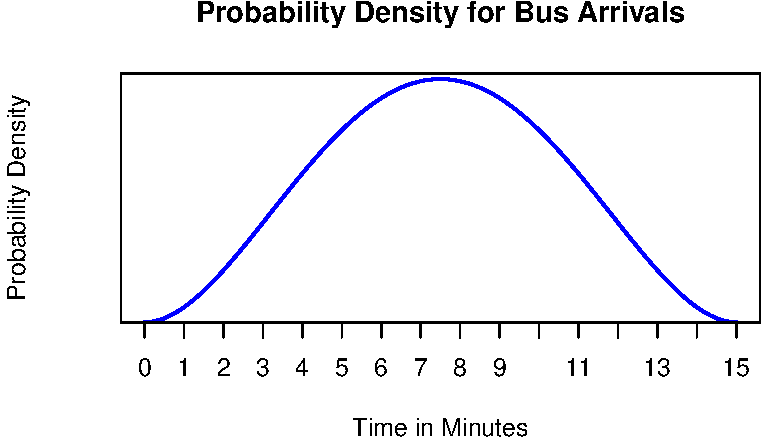
\includegraphics[keepaspectratio]{notes/chapter9_files/figure-pdf/unnamed-chunk-3-1.pdf}}

\begin{enumerate}
\def\labelenumi{\alph{enumi}.}
\tightlist
\item
  What is the value of \(\alpha\) that renders this curve a valid
  probability density function?
\item
  What is the probability that the bus arrives in the first two minutes?
\item
  What is the probability that the bus arrives in the final four
  minutes?
\end{enumerate}

\begin{tcolorbox}[enhanced jigsaw, arc=.35mm, rightrule=.15mm, breakable, bottomrule=.15mm, left=2mm, toprule=.15mm, leftrule=.75mm, opacityback=0, colback=white, colframe=quarto-callout-color-frame]

\vspace{-3mm}\textbf{Solution}\vspace{3mm}

\begin{enumerate}
\def\labelenumi{\alph{enumi}.}
\item
  We require both that the density function integrates to \(1\) and that
  it is always positive. Note that as long as \(\alpha > 0\), then
  \(f(x) \geq 0\), and so we will restrict attention only to solutions
  where \(\alpha > 0\). Beyond this, we require unit integration. That
  is, \begin{align*}
  1 &= \int_{0}^{15} \alpha \left(\frac{x}{15}\right)^2\left(1-\frac{x}{15}\right)^2dx \\
  &= 15\alpha\int_{0}^1 x^2(1 - x)^2dx \\
  &= 15\alpha\int_{0}^1 x^2(1 - 2x + x^2)dx \\
  &= 15\alpha\int_{0}^1 x^2 - 2x^3 + x^4dx \\
  &= 15\alpha\left[\frac{x^3}{3} - \frac{x^4}{2} + \frac{x^5}{5}\right]_{x=0}^1 \\
  &= 15\alpha\left[\frac{1}{3} - \frac{1}{2} + \frac{1}{5}\right] \\
  &= 15\alpha\frac{1}{30} \\
  &= \frac{\alpha}{2} \\
  \implies \alpha = 2.
  \end{align*}
\item
  The probabilities can then be derived by integrating the density over
  the given area. As an alternative solution, you can integrate the
  density to derive the cumulative distribution function, and then use
  this to solve for the probabilities. Both techniques are shown.

  To find \(F(x)\), we take \begin{align*}
       F(x) &= \int_{0}^{x}  2\left(\frac{t}{15}\right)^2\left(1-\frac{t}{15}\right)^2dt \\
       &= 30\left[\frac{t^3}{3} - \frac{t^4}{2} + \frac{t^5}{5}\right]_{t=0}^{t=x/15} \\
       &= 10\left(\frac{x}{15}\right)^3 - 15\left(\frac{x}{15}\right)^4 + 6\left(\frac{x}{15}\right)^5.
  \end{align*} Then, if we wish to find
  \[P(X \leq 2) = F(2) = 10\left(\frac{2}{15}\right)^3 - 15\left(\frac{2}{15}\right)^4 + 6\left(\frac{2}{15}\right)^5 = \frac{4864}{253125}.\]

  Alternatively, we could have solved
  \[\int_{0}^{2} 2\left(\frac{t}{15}\right)^2\left(1-\frac{t}{15}\right)^2dt = \frac{4864}{253125},\]
  directly, through the same integration steps outlined.
\item
  We can use the cumulative distribution function found previously, or
  else directly integrate. To directly integrate you would solve
  \[\int_{11}^{15} 2\left(\frac{t}{15}\right)^2\left(1-\frac{t}{15}\right)^2dt,\]
  however, given that \(F(x)\) is known it is simpler to use that. This
  is given by
  \[P(11 \leq X \leq 15) = F(15) - F(11) = 1 - F(11) = 1 - \left(10\left(\frac{11}{15}\right)^3 - 15\left(\frac{11}{15}\right)^4 + 6\left(\frac{11}{15}\right)^5\right),\]
  which gives \[P(11 \leq X \leq 15) = \frac{30848}{253125}.\]
\end{enumerate}

\end{tcolorbox}

\end{example}

\section{Using Continuous
Distributions}\label{using-continuous-distributions}

With the exception of the previously indicated differences, continuous
and discrete random variables are treated similarly. The tools to
analyze them differ\footnote{In the continuous case we cannot sum over
  the sample space, and so we must use techniques from calculus to
  mirror this process, for instance.}, but the fundamentals remain the
same. It is possible to compute expected values, medians, and modes,
with roughly the same interpretations. It is possible to describe the
range, interquartile range, and variance, with similar interpretations.
The axioms of probability still underpin the manipulation and analysis
of these random variables. The distinction is merely that in, place of
elementary mathematics to complete the calculations, calculus is
required.

\subsection{\texorpdfstring{\(\int\) Differences in Working With
Discrete and Continuous Random
Variables}{\textbackslash int Differences in Working With Discrete and Continuous Random Variables}}\label{int-differences-in-working-with-discrete-and-continuous-random-variables}

Most of what was covered for discrete random variables will hold for
continuous random variables as well, with the caveat that in the
continuous case we replace summations with integrals. We have seen this
to an extent already. In the discrete case, if a random variable \(X\)
has probability mass function \(p(x)\), then
\(P(a \leq X \leq b) = \sum_{x=a}^{b} p(x)\). Similarly, in the
continuous case, if the probability density function is \(f(x)\), then
we write \(P(a \leq X \leq b) = \sum_{a}^b f(x)dx\).

This holds across other defining identities as well, for instance
discussing the expected value or variance of a random variable. It is
worth highlighting the two major differences for working with continuous
random variables once more. First, while in the discrete case we think
predominantly of probabilities being defined on the singletons, with the
probability mass function encoding \(p(x) = P(X = x)\), these
probabilities are all zero for continuous random variables. We can make
this argument more concretely now using our technique for calculating
probabilities based on the density function, where
\[P(X = a) = P(a \leq X \leq a) = \int_{a}^{a} f(x)dx = 0.\] As a
result, no matter the value or the random variable under consideration,
we always know that \(P(X = x) = 0\) for continuous quantities.

Secondly, the density function does not directly encode probabilities,
and so can take on values greater than \(1\). As a result, when
considering the validity of a probability density function we need to
consider not the specific values of the density being bounded, but
rather the entire range.\footnote{As a note, the integrate to one and
  sum to one properties for density functions and mass functions,
  respectively, are an additional example of a situation wherein the sum
  and integral can be interchanged for one another.}

Beyond introductory courses and notes, it is quite common to discuss
only continuous random variables. In areas where both discrete and
continuous random variables are relevant, a common convention is to
simply define the integral sign in such a way so as to read it as a
summation if a discrete random variable is being used. That is, in
reading beyond these notes you may have authors express
\(\sum_{x=0}^5 p(x)\) as \(\int_{0}^5 p(x)dx\), where the summation is
implied if \(p(x)\) characterizes a discrete distribution. In these
notes we will continue separating out integrals and summations
explicitly.

\subsection{\texorpdfstring{\(\int\) Calculating Expected Values for
Continuous Random
Variables}{\textbackslash int Calculating Expected Values for Continuous Random Variables}}\label{int-calculating-expected-values-for-continuous-random-variables}

Using the convention that summations become integrals when moving from
discrete to continuous random variables, we can introduce the idea of a
continuous expected value.

\begin{definition}[Expected Value (Mean) of a Continuous Random
Variable]\protect\hypertarget{def-EV-continuous}{}\label{def-EV-continuous}

For a continuous random variable, \(X\), the expected value is
interpreted as the center of mass of the distribution. Supposing that
\(X\) has density function, \(f(x)\), then
\[E[X] = \int_{-\infty}^\infty xf(x)dx.\] When the random variable \(X\)
is defined on a bounded support \(\mathcal{X}\), the expected value can
be equivalently written as the integral only over that support
\[E[X] = \int_{\mathcal{X}} f(x)dx.\]

\end{definition}

Beyond the swapping of the summation for an integral, expected values
behave equivalently whether the underlying distribution is discrete or
continuous. That is, any of the properties relating to expected values
can be written in terms of the expectation notation, \(E[\cdot]\), with
the relevant sum or integral being computed as required. The quantities
are otherwise interpreted in the same manner as well. Notably, this
means that the Law of the Unconscious Statistician holds in the
continuous case.

\begin{tcolorbox}[enhanced jigsaw, arc=.35mm, title={The Law of the Unconscious Statistician}, rightrule=.15mm, coltitle=black, opacitybacktitle=0.6, colbacktitle=quarto-callout-tip-color!10!white, leftrule=.75mm, colback=white, breakable, titlerule=0mm, toptitle=1mm, bottomtitle=1mm, bottomrule=.15mm, toprule=.15mm, opacityback=0, left=2mm, colframe=quarto-callout-tip-color-frame]

The law of the unconscious statistician (LOTUS) states that, for a
random variable \(X\), if we wish to find \(E[g(X)]\), then we compute
\[E[g(X)] = \int_{-\infty}^\infty g(x)f_X(x)dx.\]

\end{tcolorbox}

Using the continuous version of the LOTUS, we can define the following
quantities which parallel their discrete counterparts.

\begin{tcolorbox}[enhanced jigsaw, arc=.35mm, title={Expected Value of a Linear Transformation}, rightrule=.15mm, coltitle=black, opacitybacktitle=0.6, colbacktitle=quarto-callout-tip-color!10!white, leftrule=.75mm, colback=white, breakable, titlerule=0mm, toptitle=1mm, bottomtitle=1mm, bottomrule=.15mm, toprule=.15mm, opacityback=0, left=2mm, colframe=quarto-callout-tip-color-frame]

If \(a\) and \(b\) are arbitrary real numbers then,
\[E[aX + b] = aE[X] + b.\]

\end{tcolorbox}

\begin{definition}[Variance]\protect\hypertarget{def-variance-continuous}{}\label{def-variance-continuous}

The variance of a random variable, typically denoted \(\text{var}(X)\),
is given by the expected value of the squared deviations of a random
variable from its mean. That is,
\[\text{var}(X) = E\left[(X - E[X])^2\right].\]

\end{definition}

\begin{tcolorbox}[enhanced jigsaw, arc=.35mm, title={Computing the Variance}, rightrule=.15mm, coltitle=black, opacitybacktitle=0.6, colbacktitle=quarto-callout-tip-color!10!white, leftrule=.75mm, colback=white, breakable, titlerule=0mm, toptitle=1mm, bottomtitle=1mm, bottomrule=.15mm, toprule=.15mm, opacityback=0, left=2mm, colframe=quarto-callout-tip-color-frame]

The variance of a random variable, \(X\), can be computed as
\[\text{var}(X) = E[(X - E[X])^2] = E[X^2] - E[X]^2.\]

\end{tcolorbox}

\begin{tcolorbox}[enhanced jigsaw, arc=.35mm, title={Variance of a Linear Transformation}, rightrule=.15mm, coltitle=black, opacitybacktitle=0.6, colbacktitle=quarto-callout-tip-color!10!white, leftrule=.75mm, colback=white, breakable, titlerule=0mm, toptitle=1mm, bottomtitle=1mm, bottomrule=.15mm, toprule=.15mm, opacityback=0, left=2mm, colframe=quarto-callout-tip-color-frame]

If \(a\) and \(b\) are arbitrary real numbers then,
\[\text{var}[aX + b] = a^2\text{var}(X).\]

\end{tcolorbox}

\begin{definition}[Standard
Deviation]\protect\hypertarget{def-sd-continuous}{}\label{def-sd-continuous}

The standard deviation of a random variable is the square root of the
variance, which is to say \[\text{SD}(X) = \sqrt{\text{var}(X)}.\]

\end{definition}

\begin{example}[Charles and Sadie Potato
Yield]\protect\hypertarget{exm-expectations-for-crvs}{}\label{exm-expectations-for-crvs}

Charles and Sadie have purchased a plot of land and they are looking to
do some sustainable development of it. In their planning, they are
looking at different crops that they could grow. Charles and Sadie
decide that potatoes sound particularly fun, and do some research into
the amount that they can anticipate from each plant. From their research
they find that the probability density function for single plant potato
yield (in pounds) is given by
\[f(x) = \frac{25}{52}\exp\left(-\frac{25x}{52}\right) \quad x \geq 0.\]

\begin{enumerate}
\def\labelenumi{\alph{enumi}.}
\tightlist
\item
  What is the expected yield, in pounds, for a single potato plant?
\item
  What is the variance and standard deviation for the yield for a single
  potato plant?
\item
  While Sadie is happy to work in pounds, Charles much prefers
  kilograms. Moreover, the yield given by the previous distribution
  function was over counting by \(0.2\)lbs per plant, since they had not
  considered the dirt that came with the harvest. What is the actual
  expected value, variance, and standard deviation for the total yield
  in kilograms (note, \(1\) kilogram is \(2.2\) pounds).
\end{enumerate}

\begin{tcolorbox}[enhanced jigsaw, arc=.35mm, rightrule=.15mm, breakable, bottomrule=.15mm, left=2mm, toprule=.15mm, leftrule=.75mm, opacityback=0, colback=white, colframe=quarto-callout-color-frame]

\vspace{-3mm}\textbf{Solution}\vspace{3mm}

\begin{enumerate}
\def\labelenumi{\alph{enumi}.}
\item
  To get the expected yield we find
  \[E[X] = \int_{0}^\infty xf(x)dx = \int_{0}^\infty x\frac{25}{52}\exp\left(-\frac{25x}{52}\right)dx.\]
  This can be solved via integration by parts as \begin{align*}
  E[X] &= \int_{0}^\infty x\frac{25}{52}\exp\left(-\frac{25x}{52}\right)dx \\
  &= \left[-x\exp\left(-\frac{25x}{52}\right)\right]_{x=0}^\infty + \int_{0}^\infty \exp\left(-\frac{25x}{52}\right)dx \\
  &= 0+\left[-\frac{52}{25}\exp\left(-\frac{25x}{52}\right)\right]_{x=0}^\infty \\
  &= \frac{52}{25}.
  \end{align*}
\item
  For the variance, we can use the fact that
  \(\text{var}(X) = E[X^2] - E[X]^2\). Note that \(E[X^2]\) can be
  computed in much the same way as \(E[X]\), requiring two applications
  of integration by parts, \begin{align*}
  E[X^2] &= \int_{0}^\infty x^2\frac{25}{52}\exp\left(-\frac{25x}{52}\right)dx \\
  &= \left[x^2\exp\left(-\frac{25x}{52}\right)\right]_{x=0}^\infty + 2\int_{0}^\infty x\exp\left(-\frac{25x}{52}\right) \\
  &= 2\int_{0}^\infty x\exp\left(-\frac{25x}{52}\right) \\
  &= 2\times\frac{52}{25}\times\int_{0}^\infty x\frac{25}{52}\exp\left(-\frac{25x}{52}\right) \\
  &= \frac{104}{25}\times E[X] \\
  &= \frac{104}{25}\times\frac{52}{25}.
  \end{align*} Thus,
  \[\text{var}(X) = \frac{104}{25}\times\frac{52}{25} - \left(\frac{52}{25}\right)^2 = \left(\frac{52}{25}\right)^2.\]
  As a result, \(\text{SD}(X) = E[X] = \frac{52}{25}\).
\item
  If \(X\) is the weight in pounds, then the new weight will be
  \[Y = frac{(X - 0.2)}{2.2} = \frac{1}{2.2}X - \frac{1}{11}.\] Then, we
  can apply the linear transformation theorems to get
  \[E[Y] = \frac{1}{2.2}E[X] - \frac{1}{11} = \frac{47}{55}.\]
  Similarly, we have
  \[\text{var}(Y) = \frac{1}{2.2^2}\text{var}(X) = \frac{2704}{3025}.\]
  This leads to a standard deviation of
  \[\text{SD}(X) = \frac{52}{55}.\]
\end{enumerate}

\end{tcolorbox}

\end{example}

\subsection{\texorpdfstring{\(\int\) Calculating Percentiles for
Continuous Random
Variables}{\textbackslash int Calculating Percentiles for Continuous Random Variables}}\label{int-calculating-percentiles-for-continuous-random-variables}

In the same way that expected values generalized from the discrete to
the continuous case, so too will percentiles.

\begin{definition}[Percentiles]\protect\hypertarget{def-percentile-continuous}{}\label{def-percentile-continuous}

The \(100p\)th percentile, is denoted \(\zeta(p)\) and is the value such
that \(P(X \leq \zeta(p)) = p\). Thus, the median is given by
\(\zeta(0.5)\) and is also called the \(50\)th percentile.

\end{definition}

A key distinction between percentiles in discrete case as compared to
the continuous case is that, in the discrete case, it was often not
possible to find \(\zeta(p)\) such that \(P(X \leq \zeta(p)) = p\) held
exactly. Instead, we found \(\zeta(p)\) such that
\(P(X \leq \zeta(p)) \geq p\) and \(P(X \geq \zeta(p)) \geq p\). In the
continuous case, this is not typically required. This gives two
(equivalent) techniques for solving for a given percentile using
continuous distributions. If the cumulative distribution function,
\(F(x)\), is known then \(\zeta(p) = F^{-1}(p)\).\footnote{When \(F\) is
  not strictly invertible, we can instead consider the generalized
  inverse based on the right-continuity of \(F\), giving
  \(F^{-1}(p) = \inf\{x\in\mathbb{R}\mid p \leq F(x)\}\).}

Alternatively, we can work from the density function directly and solve
the integral equation, \[\int_{-\infty}^{\zeta(p)} f(x)dx = p,\] for
\(\zeta(p)\). Doing so implicitly works out the cumulative distribution
function as an intermediate step, however, there are cases where there
is no closed-form solution for the cumulative distribution function but
this technique can still be used.

Given the definition of a percentile in the continuous case, we can
introduce both the median and the interquartile range as being exactly
analogous to the quantities in the discrete case.

\begin{definition}[Median
(Continuous)]\protect\hypertarget{def-median-continuous}{}\label{def-median-continuous}

The median of a distribution is the \(50\)th percentile, \(\zeta(0.5)\).
That is, the median \(m\) is the value such that \(P(X \leq m) = 0.5\).

\end{definition}

\begin{definition}[Interquartile Range
(IQR)]\protect\hypertarget{def-iqr-continuous}{}\label{def-iqr-continuous}

The interquartile range, or IQR, is defined as
\(\zeta(0.75) - \zeta(0.25)\), the difference between the third and
first quartiles. It is a measure of spread, and is typically denoted as
\(\text{IQR} = Q3 - Q1\), where \(Q\) stands for quartiles.

\end{definition}

\begin{example}[Median Potato
Yield]\protect\hypertarget{exm-expectations-for-crvs}{}\label{exm-expectations-for-crvs}

Still interested in the potatoes that they could grow on their land,
Charles and Sadie want to further investigate what they should expect
for the potatoes that they grow. While they now understand the mean and
variance, they figure that it is probably worth understanding the median
and interquartile range as well, as this may give a better capacity to
plan for the best and worst case scenarios. Suppose that the probability
density function for single plant potato yield (in pounds) is given by
\[f(x) = \frac{25}{52}\exp\left(-\frac{25x}{52}\right) \quad x \geq 0.\]

\begin{enumerate}
\def\labelenumi{\alph{enumi}.}
\tightlist
\item
  What is the median yield for a single potato plant?
\item
  What is the interquartile range for the yield of a single potato
  plant?
\end{enumerate}

\begin{tcolorbox}[enhanced jigsaw, arc=.35mm, rightrule=.15mm, breakable, bottomrule=.15mm, left=2mm, toprule=.15mm, leftrule=.75mm, opacityback=0, colback=white, colframe=quarto-callout-color-frame]

\vspace{-3mm}\textbf{Solution}\vspace{3mm}

\begin{enumerate}
\def\labelenumi{\alph{enumi}.}
\item
  For the median we need to solve \(F(x) = 0.5\) for \(x\). We could do
  this direct from the integral, or by first finding the cumulative
  distribution function. We will first find the cumulative distribution
  function to ease the efforts required for the interquartile range
  calculation. Note that
  \[F(x) = \int_{0}^x \frac{25}{52}\exp\left(-\frac{25t}{52}\right)dt = \left[-\exp\left(-\frac{25t}{52}\right)\right]_{t=0}^{x} = 1 - \exp\left(-\frac{25x}{52}\right).\]
  Then, we get \begin{align*}
  0.5 &= 1 - \exp\left(-\frac{25x}{52}\right) \\
  0.5 &= \exp\left(-\frac{25x}{52}\right) \\
  \log(0.5) &= -\frac{25x}{52} \\ 
  x &= \frac{52}{25}\log(2) \\
  &\approx 1.442.
  \end{align*}
\item
  The IQR first requires Q1 and Q3. Thus, we solve these in the same way
  as above. In fact, for general percentile we get \begin{align*}
  p &= 1 - \exp\left(-\frac{25x}{52}\right) \\
  1-p &= \exp\left(-\frac{25x}{52}\right) \\
  \log(1-p) &= -\frac{25x}{52} \\ 
  x &= \frac{52}{25}\log(\frac{1}{1-p}).
  \end{align*} Thus, we have
  \[\text{IQR} = \frac{52}{25}\log(\frac{1}{0.25}) - \frac{52}{25}\log(\frac{1}{0.75}) \approx 2.2851.\]
\end{enumerate}

\end{tcolorbox}

\end{example}

\subsection{The Named Continuous
Distributions}\label{the-named-continuous-distributions}

Just as with discrete distributions, there are named continuous
distributions. These are typically governed by either a density function
or cumulative distribution function, alongside the expected value and
variance. Just like the named discrete distributions, by matching the
underlying scenario to the correct process we are able to avoid a lot of
work in understanding the behaviour of the random quantities. Now,
because calculus is not assumed knowledge, we will not work too widely
with continuous random variables. We will introduce several named
continuous distributions: the uniform distribution\footnote{Which we
  have actually already seen.}, the normal distribution,\footnote{Which
  is far and away the most important distribution (discrete or
  continuous) in all of probability and statistics.} as well as the
\(t\), exponential and gamma distributions.\footnote{The exponential is
  actually a special case of the gamma distribution, as are several
  other important named distributions, which will be brought up as
  required.}

\section{The Uniform Distribution}\label{the-uniform-distribution}

The uniform distribution\footnote{Sometimes called the continuous
  uniform distribution to distinguish it from its discrete counterpart.}
is parameterized over an interval specified as \((a,b)\). On this
interval, equal probability density is given to every event, which is to
say that the density function is constant. Specifically, if
\(X\sim\text{Unif}(a,b)\) then
\[f(x) = \begin{cases}\frac{1}{b-a} & x \in (a,b) \\ 0 & \text{otherwise}.\end{cases}\]
From the density function we can find that
\[F(x) = \frac{x - a}{b - a}\] for \(x \in (a,b)\), with \(F(x) = 0\)
for \(x < a\) and \(F(x) = 1\) for \(x > b\). Moreover, we have
\(E[X] = \frac{a+b}{2}\) and \(\text{var}(X) = \frac{(b-a)^2}{12}\).

\begin{example}[Characterizing the Wait
Time]\protect\hypertarget{exm-charles-and-sadie-bus-times-expected}{}\label{exm-charles-and-sadie-bus-times-expected}

Still considering the wait time for buses in the city, Sadie points out
that the bus they were waiting for follows a \(\text{Unif}(0,15)\)
distribution. They can use their newfound wisdom to make deeper
conclusions about the process!\footnote{In
  Example~\ref{exm-charles-and-sadie-bus-times} we implicitly used the
  cumulative distribution function of the uniform. It is worth
  revisiting these probabilities \emph{knowing} that this is the case.}

\begin{enumerate}
\def\labelenumi{\alph{enumi}.}
\tightlist
\item
  How long should they expect to wait for the bus?
\item
  What is the variance for the amount of time that they will be waiting?
\end{enumerate}

\begin{tcolorbox}[enhanced jigsaw, arc=.35mm, rightrule=.15mm, breakable, bottomrule=.15mm, left=2mm, toprule=.15mm, leftrule=.75mm, opacityback=0, colback=white, colframe=quarto-callout-color-frame]

\vspace{-3mm}\textbf{Solution}\vspace{3mm}

Here, we know that \(X\sim\text{Unif}(0,15)\).

\begin{enumerate}
\def\labelenumi{\alph{enumi}.}
\tightlist
\item
  \(E[X]\) is \(\dfrac{a+b}{2} = \dfrac{0+15}{2} = 7.5\), so they should
  expect to wait \(7.5\) minutes.
\item
  The variance is \(\text{var}(X) = \dfrac{(15 - 0)^2}{12} = 18.75\).
\end{enumerate}

\end{tcolorbox}

\end{example}

The uniform distribution is analogous to the discrete uniform. Any time
there is an interval of possible outcomes which are all equally likely,
the uniform distribution is the distribution to use. Compared with other
distributions it is also fairly straightforward to work with, which
makes it a useful demonstration of the concepts relating the continuous
probability calculations.\footnote{For instance, in
  Example~\ref{exm-geometric}, we implicitly used a continuous uniform
  distribution to give the probability that Charles hits the dartboard.
  This type of reasoning is very prevalent.}

\section{The Normal Distribution}\label{the-normal-distribution}

The normal distribution, also sometimes referred to as the Gaussian
distribution, is a named continuous distribution function defined on the
complete real line. The distribution is far and away the most
prominently used distribution in all of probability and statistics. In
fact, most people have heard of normal distributions even if they are
not aware of this fact. Any time that there is a discussion of a bell
curve, for instance, this is in reference to the normal distribution.
Normally distributed quantities arise all over the place from
measurements of heights, grades, or reaction times through to levels of
job satisfaction, reading ability, or blood pressure. There is a
tremendous number of normally distributed phenomena naturally occurring
in the world, which renders the normal distribution deeply important
across a wide range of domains.

Perhaps more important than the places where the normal distribution
arises in nature are the places where it arises mathematically. Later in
these notes we will see a result, \emph{the central limit theorem},
which is one of the core results in all of statistics. Much of the
statistical theory that drives scientific inquiry sits atop the central
limit theorem. And at the core of the central limit theorem is the
normal distribution. It is virtually impossible to overstate the
importance of the normal distribution, and as a result, it is worthy of
investigation.

\subsection{The Specification of the
Distribution}\label{the-specification-of-the-distribution}

A normal distribution is parameterized by two parameters: the mean,
\(\mu\), and the variance \(\sigma^2\). We write
\(X\sim N(\mu,\sigma^2)\). These parameters directly correspond to the
relevant quantities such that \(E[X] = \mu\) and
\(\text{var}(X) = \sigma^2\). The density function is given by
\[f(x) = \frac{1}{\sqrt{2\pi}\sigma}\exp\left(-\frac{(x-\mu)^2}{2\sigma^2}\right).\]
This can be quite unwieldy to work with, however, when it is plotted we
see that the normal distribution takes on a bell curve which is centered
at \(\mu\).

\begin{figure}[H]

\caption{\label{fig-normal-density}Three normal distribution densities
plotted with mean 0 (red and blue), and mean 5 (black). The red density
has variance 1, the blue density has variance 4, and the black density
has variance 0.25.}

\centering{

\pandocbounded{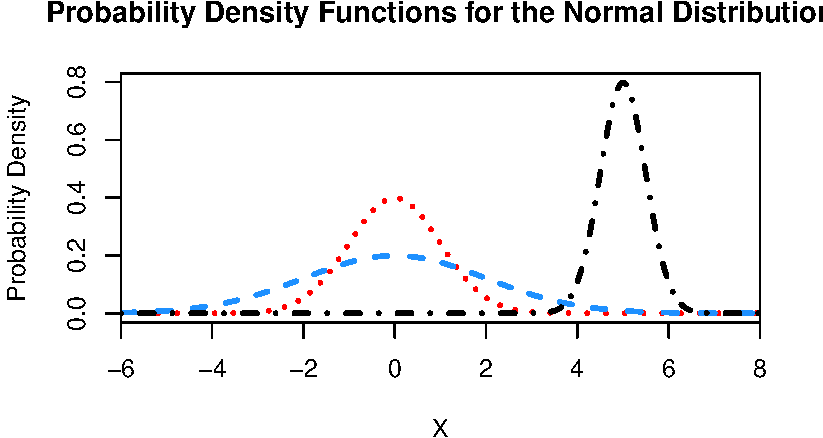
\includegraphics[keepaspectratio]{notes/chapter9_files/figure-pdf/fig-normal-density-1.pdf}}

}

\end{figure}%

\subsection{The Standard Normal
Distribution}\label{the-standard-normal-distribution}

Normally distributed random variables are particularly well-behaved. One
way in which this is true is that if you multiply a normally distributed
random variable by a constant, it will remain normally distributed, and
if you add a constant to a normally distributed random variable, it will
remain normally distributed. Consider, for \(X\sim N(\mu,\sigma^2)\),
taking the \(X - \mu\). From our discussions of expected values we know
that \(E[X-\mu] = E[X]-\mu = 0\). Furthermore, adding or subtracting a
constant will not change the variance. Thus,
\(X-\mu\sim N(0,\sigma^2)\).

Now, consider dividing this by \(\sigma\), or equivalently, multiply by
\(\dfrac{1}{\sigma}\). The expected value of the new quantity will be
\(\dfrac{1}{\sigma}\times 0 = 0\), and, from our discussions regarding
the variance of linear transformations, the variance of the new quantity
will be \(\frac{1}{\sigma^2}\times\sigma^2 = 1\). Taken together then,
if \(X\sim N(\mu,\sigma^2)\),
\[Z = \frac{X - \mu}{\sigma} \sim N(0,1).\] This holds true for
\emph{any} normal distribution with \emph{any} mean or variance values.
This straightforward transformation allows us to discuss normal
distributions in terms of \(N(0,1)\). We call this the \textbf{standard
normal distribution}, and will typically use \(Z\) to denote a random
variable from the standard normal distribution.

\begin{definition}[Standard Normal
Distribution]\protect\hypertarget{def-standard-normal}{}\label{def-standard-normal}

The standard normal distribution is the version of the normal
distribution with mean \(0\) and variance \(1\). We say that \(Z\)
follows a standard normal, and write \(Z\sim N(0,1)\), if the density of
\(Z\) is given by
\[f_Z(z) = \frac{1}{\sqrt{2\pi}}\exp\left(-\frac{z^2}{2}\right).\] We
denote the density of \(Z\) as \(\varphi(z)\), and the cumulative
distribution function of \(Z\) as \(\Phi(z)\). The cumulative
distribution function, \(\Phi(z)\), does not have a nice form to be
written down, however, it is a commonly applied enough function that
many computing languages have implemented it, including of course
R.\footnote{See Section~\ref{sec-r-continuous} for more details on this.}

\end{definition}

The utility in this process of converting normally distributed random
variables to be standard normal random variables, a process known as
\textbf{standardization}, is demonstrated by realizing that events can
be converted using the same transformations. Specifically, suppose we
have \(X \sim N(\mu,\sigma^2)\), and we want to find \(P(X \leq x)\).
Note that, \(X \leq x\) must also mean that
\[\frac{X-\mu}{\sigma} \leq \frac{x - \mu}{\sigma},\] through an
application of the same transformation to both sides. But we \emph{know}
that the left hand side of this inequality is exactly \(Z\), a standard
normal random variable with cumulative distribution function
\(\Phi(z)\). Thus,
\[P(X \leq x) = P\left(Z \leq \frac{x - \mu}{\sigma}\right) = \Phi\left(\frac{x-\mu}{\sigma}\right).\]
Using this trick of standardization any normal probability can be
converted into a probability regarding the standard normal.

\begin{example}[Charles and Sadie Explore House
Plants]\protect\hypertarget{exm-standardization-example}{}\label{exm-standardization-example}

Charles and Sadie learn that the heights of fully grown house plants are
often normally distributed. They are exploring which plants will work
best in their new apartment, but are finding it difficult to reason
about them in comparison to one another. Some plants end up being taller
on average with a lot more variability, while others may be shorter but
far more certain. Sadie realizes that the cumulative distribution
function of a standard normal, \(\Phi(z)\), can be evaluated using their
smart phones. As a result, they get to work expressing different
probabilities in terms of \(\Phi(z)\).

They are comparing four different plant species. These species have
heights according to the following random variables.

\begin{enumerate}
\def\labelenumi{\roman{enumi}.}
\tightlist
\item
  Plant \(A\) has height \(X\), which follows a normal distribution with
  mean \(90\) and variance \(100\).
\item
  Plant \(B\) has height \(Y\), which follows a \(N(110, 400)\)
  distribution.
\item
  Plant \(C\) has height \(V\), which follows a normal distribution
  centered on \(70\) with standard deviation \(7\).
\item
  Plant \(D\) has height \(W\), which follows a normal distribution with
  \(\mu=85\) and \(\sigma^2 = 81\).
\end{enumerate}

Express each of the following probabilities in terms of \(\Phi(z)\), the
cumulative distribution function of a standard normal random variable.

\begin{enumerate}
\def\labelenumi{\alph{enumi}.}
\tightlist
\item
  One spot the plants cannot be too tall. What is the probability that
  they can fit plant \(A\) into a spot which cannot accommodate plants
  taller than \(80\)cm?
\item
  A second spot would be strange to have too short of a plant in. If
  they require the plant to be at least \(125\)cm, what is the
  probability they can use plant \(B\)?
\item
  A third spot can accommodate plants that are either under \(60\)cm if
  they use a stand, or else over \(90\)cm. How likely is it that plant
  \(C\) will work in this spot?
\item
  A fourth spot requires a plant that is somewhere between \(80\)cm and
  \(90\)cm. What is the probability that plant \(D\) will work?
\end{enumerate}

\begin{tcolorbox}[enhanced jigsaw, arc=.35mm, rightrule=.15mm, breakable, bottomrule=.15mm, left=2mm, toprule=.15mm, leftrule=.75mm, opacityback=0, colback=white, colframe=quarto-callout-color-frame]

\vspace{-3mm}\textbf{Solution}\vspace{3mm}

\begin{enumerate}
\def\labelenumi{\alph{enumi}.}
\tightlist
\item
  Here we wish to standard a \(N(90, 100)\) random variable. To do this
  we note that
  \[\frac{X-90}{\sqrt{100}} = \frac{X - 90}{10} \sim N(0,1).\] Thus,
  taking \(Z \sim N(0,1)\), we know that
  \[P(X \leq 80) = P\left(\frac{X - 90}{10} \leq \frac{80 - 90}{10}\right) = P(Z \leq -1) = \Phi(-1).\]
\item
  Here we wish to standard a \(N(110, 400)\) random variable. To do this
  we note that
  \[\frac{Y-110}{\sqrt{400}} = \frac{Y - 110}{20} \sim N(0,1).\] Thus,
  taking \(Z \sim N(0,1)\), we know that
  \[P(Y \geq 125) = P\left(\frac{Y - 110}{20} \geq \frac{125 - 110}{20}\right) = P(Z \geq \frac{3}{4}) = 1 - \Phi(0.75).\]
\item
  Here we wish to standard a \(N(70, 49)\) random variable. To do this
  we note that \[\frac{V-70}{7} \sim N(0,1).\] Thus, taking
  \(Z \sim N(0,1)\), we know that
  \[P(V \leq 60) = P\left(\frac{V - 70}{7} \leq \frac{60 - 70}{7}\right) = P(Z \leq -\frac{10}{7}) = \Phi(-\frac{10}{7}).\]
  Moreover, we know that
  \[P(V \geq 90) = P\left(\frac{V - 70}{7} \geq \frac{90 - 70}{7}\right) = P(Z \geq \frac{20}{7}) = 1 - \Phi(\frac{20}{7}).\]
  Thus, the probability this will be acceptable will be
  \(1 - \Phi(\frac{20}{7}) + \Phi(-\frac{10}{7})\).
\item
  Here we wish to standard a \(N(85, 81)\) random variable. To do this
  we note that
  \[\frac{W-85}{\sqrt{81}} = \frac{W - 85}{9} \sim N(0,1).\] Thus,
  taking \(Z \sim N(0,1)\), we know that
  \begin{multline*}P(80 \leq W \leq 90) = P\left(\frac{80 - 85}{9} \leq \frac{W - 85}{9} \leq \frac{90 - 85}{9}\right) \\ = P(Z \leq \frac{5}{9}) - P(Z \leq -\frac{5}{9}) = \Phi(\frac{5}{9}) - \Phi(-\frac{5}{9}).\end{multline*}
\end{enumerate}

\end{tcolorbox}

\end{example}

As a result, combining our knowledge of continuous random variables,
with the process of standardization we are able to calculate normal
probabilities for any events relating to normally distributed random
quantities. Moreover, since the shape of the normal distribution is so
predictable, it is often easy to draw out the density function, and
indicate on this graphic the probabilities of interest, which in turn
helps with the required probability calculations. Calculating
probabilities from normal distributions remains a central component of
working with statistics and probabilities beyond these notes. Developing
the skills and intuition at this point, through repeated practice is a
key step in successfully navigating statistics here and beyond.

When you have access to a computer, and your interest is in calculating
a normal probability, as described above, there is not typically a need
for standardization. However, it remains an important skill for several
reasons. First, by always working with the same normal distribution, you
will develop a much more refined intuition for the likelihoods of
different events. It goes beyond working with the same family of
distributions, you get very used to working with exactly the same
distribution. Second, you will likely become quite familiar with certain
key \textbf{critical values} of the standard normal distribution. These
values arise frequently, and allow you to quickly approximate the
likelihood of different events. Finally, as we begin to move away from
studying probability and into studying statistics, the standard normal
will feature prominently there.

\subsection{The Empirical Rule and Chebyshev's
Inequality}\label{the-empirical-rule-and-chebyshevs-inequality}

Another way in which the normal distribution is well behaved is
summarized in the \textbf{emprical rule}. The shape of the distribution
is such that, no matter the specific mean or variance, all members of
the family remain quite similar. This enables the derivation of an easy,
approximate result, to help intuitively gauge the probabilities of
normal events.

\begin{tcolorbox}[enhanced jigsaw, arc=.35mm, title={The Empirical Rule}, rightrule=.15mm, coltitle=black, opacitybacktitle=0.6, colbacktitle=quarto-callout-tip-color!10!white, leftrule=.75mm, colback=white, breakable, titlerule=0mm, toptitle=1mm, bottomtitle=1mm, bottomrule=.15mm, toprule=.15mm, opacityback=0, left=2mm, colframe=quarto-callout-tip-color-frame]

The empirical rule is a mathematical result regarding the probability of
a normally distributed random variable. If \(X\) has a normal
distribution with mean \(\mu\) and variance \(\sigma^2\), then:

\begin{enumerate}
\def\labelenumi{\arabic{enumi}.}
\tightlist
\item
  The probability of observing a value within \(\sigma\) of the mean is
  approximately \(0.68\);
\item
  The probability of observing a value within \(2\sigma\) of the mean is
  approximately \(0.95\); and
\item
  The probability of observing a value within \(3\sigma\) of the mean is
  approximately \(0.997\).
\end{enumerate}

\pandocbounded{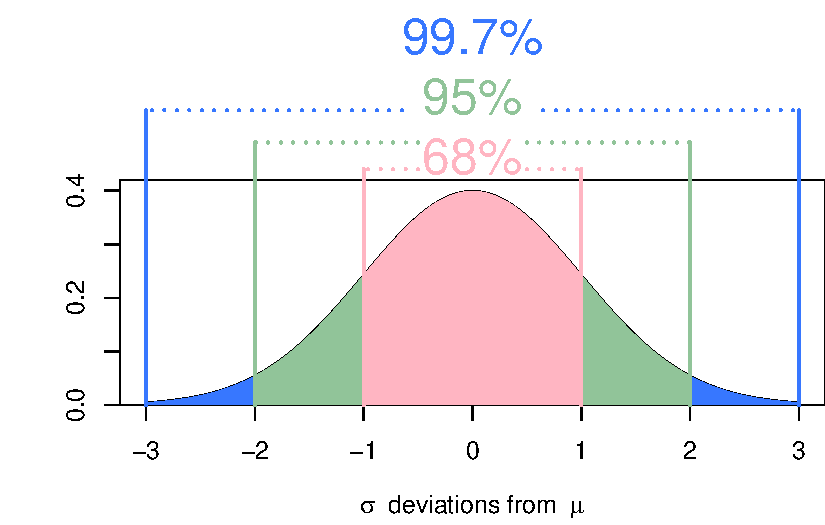
\includegraphics[keepaspectratio]{notes/chapter9_files/figure-pdf/empirical_rule-1.pdf}}

\end{tcolorbox}

In words, the empirical states that almost all of the observations from
a normal distribution will fall in the interval \(\mu\pm3\sigma\). In
mathematical terms, the empirical rule is summarized as \begin{align*}
    P(\mu-\sigma\leq X \leq \mu + \sigma) &\approx 0.68 \\ 
    P(\mu - 2\sigma \leq X \leq \mu + 2\sigma) &\approx 0.95 \\ 
    P(\mu - 3\sigma \leq X \leq \mu + 3\sigma) &\approx 0.997. 
\end{align*} With the standard normal we can replace \(\mu\) with \(0\),
and \(\sigma\) with \(1\) to get a version which is slightly more
concise to state. It is then possible to combine these different
intervals by recognizing the symmetry in the normal distribution. That
is, \(P(\mu \leq X \leq \mu + \sigma) \approx \dfrac{0.68}{2} = 0.34\).

\begin{example}[Charles and Sadie Can Never Have Enough House
Plants]\protect\hypertarget{exm-empirical-rule-calc}{}\label{exm-empirical-rule-calc}

Their standardization efforts paid off, and Charles and Sadie found some
plants that should fit the spaces that they need once they've grown up.
Because of how well the plants worked out, they wanted to buy some more.
They end up back at the store, and they know that they need to get a
plant that will grow to be between \(70\)cm and \(106\)cm. They have
several options for plants again:

\begin{enumerate}
\def\labelenumi{\roman{enumi}.}
\tightlist
\item
  A plant with heights \(X\) according to \(N(88, 36)\).
\item
  A plant with heights \(Y\) according to \(N(124, 324)\).
\item
  A plant with heights \(W\) according to \(N(82, 144)\).
\end{enumerate}

Unfortunately, Charles and Sadie forget their phones at home and so they
cannot make direct calculations using \(\Phi(z)\). Can you help them,
without using a normal probability calculator, determine which plant has
the highest probability of being acceptable?

\begin{tcolorbox}[enhanced jigsaw, arc=.35mm, rightrule=.15mm, breakable, bottomrule=.15mm, left=2mm, toprule=.15mm, leftrule=.75mm, opacityback=0, colback=white, colframe=quarto-callout-color-frame]

\vspace{-3mm}\textbf{Solution}\vspace{3mm}

Without access to \(\Phi(z)\) we can instead make use of the empirical
rule. Consider that for \(X\) we have \(\mu_X = 88\) and
\(\sigma = \sqrt{36} = 6\).

\begin{enumerate}
\def\labelenumi{\arabic{enumi}.}
\tightlist
\item
  If we take the interval \([70, 106]\) then we can consider the terms
  \[\frac{70-88}{6} = \frac{-18}{6} = -3 \quad\text{and}\quad \frac{106-88}{6} = 3.\]
  Thus,
  \(P(70 \leq X \leq 106) = P(\mu_X - 3\sigma_X \leq X \leq \mu_X + 3\sigma_X)\).
  Using the empirical rule we know that this probability is
  approximately \(0.997\).
\item
  We can approach the same tactics for \(Y\). This time, we get
  \[\frac{70-124}{\sqrt{324}} = -3 \quad\text{and}\quad \frac{106-124}{18} = -1\].
  Thus,
  \(P(70 \leq Y \leq 106) = P(\mu_Y - 3\sigma_Y \leq Y \leq \mu_Y - \sigma_Y)\).
  Note that from \(\mu\) to \(\mu-3\sigma\), according the empirical
  rule, there is \(\dfrac{0.997}{2} = 0.4985\) probability. Similarly,
  according to the empirical rule there is \(\dfrac{0.68}{2} = 0.34\)
  probability of being between \(\mu\) and \(\mu-\sigma\). Thus, if we
  take \(0.4985 - 0.34 = 0.1585\), this gives the probability of being
  between \(\mu-3\sigma\) and \(\mu-\sigma\), as required.
\item
  As above,
  \[\frac{70-82}{\sqrt{144}} = -1 \quad\text{and}\quad \frac{106-82}{12} = 2\].
  As a result,
  \(P(70 \leq W \leq 106) = P(\mu_W - \sigma_W \leq W \leq \mu_W + 2\sigma_W)\).
  Note that as in (2) there is \(0.34\) probability of being between
  \(\mu\) and \(\mu-\sigma\). To be between \(\mu\) and
  \(\mu + 2\sigma\) there will be probability
  \(\dfrac{0.95}{2} = 0.475\). As a result, the total probability here
  will be \(0.34 + 0.475 = 0.815\).
\end{enumerate}

As a result, the first plant has a \(0.997\) chance to fit, the second a
\(0.1585\), and the third a \(0.815\) (approximately).

\end{tcolorbox}

\end{example}

The empirical rule is not exact, and when computing probabilities with
access to statistical software it is likely of limited direct utility.
However, it is another tool to leverage to continue refining your
intuition for the behaviour of random quantities. It is also a good
``check'' to have, giving an immediate sense of the likelihood of
different events. If you compute an answer which seems to contradict the
empirical rule, take a second look. If you have someone tell you that
they have observed events which are out of line with the empirical rule,
be skeptical.

The empirical rule is a useful result to aid in building intuition
regarding the normal distribution. However, when quantities are not
normally distributed, it does not apply. A related, though somewhat
weaker result is Chebyshev's Inequality. This will hold for \emph{any}
distribution, and can be seen as a useful extension to the empirical
rule.

\begin{tcolorbox}[enhanced jigsaw, arc=.35mm, title={Chebyshev's Inequality}, rightrule=.15mm, coltitle=black, opacitybacktitle=0.6, colbacktitle=quarto-callout-tip-color!10!white, leftrule=.75mm, colback=white, breakable, titlerule=0mm, toptitle=1mm, bottomtitle=1mm, bottomrule=.15mm, toprule=.15mm, opacityback=0, left=2mm, colframe=quarto-callout-tip-color-frame]

Chebyshev's Inequality provides probabilistic bounds on the likelihood
of deviating from the mean for any random variable. In words, there is a
probability of \(0.75\) or more of observing an observation within two
standard deviations, and a probability of at least \(0.8889\) of
observing a value within three standard deviations of the mean.
Formally, for any \(k > 0\),
\[P(\mu - k\sigma \leq X \leq \mu + k\sigma) \geq 1 - \frac{1}{k^2}.\]

\end{tcolorbox}

Here \(k\) can be any real number which is greater than \(0\). If
\(k\leq 1\), this result is uninteresting since the bound simply is
\(0\). However, taking \(k=2\) gives the \(0.75\) lower bound outlined
above, which is a more useful result. Additionally, there is no
requirement for \(k\) to be an integer here, and so, for instance, the
probability of observing a value within \(\mu\pm\sqrt{2}\sigma\) is at
least \(0.5\), for all distributions.

\begin{example}[Fitting in the Strange
Plants]\protect\hypertarget{exm-chebyshevs-ineqaulity}{}\label{exm-chebyshevs-ineqaulity}

Charles and Sadie selected a plant to fit in the spot requiring one
between \(70\) and \(106\)cm. However, as they are checking out at the
store they see a plant that they like much better. They are conflicted
since they do not know whether this plant will satisfy normality
assumptions in its height. The worker tells them that on average the
plant grows to be \(88\)cm, and figures that the variance will be
approximately \(51.84\). Charles and Sadie want to be at least \(90\%\)
certain that the plant will fit. If they are, they will buy it!

\begin{enumerate}
\def\labelenumi{\alph{enumi}.}
\tightlist
\item
  If they assume that the plants heights are normally distributed,
  should they buy the plant?
\item
  If they do not assume that the plants heights are normally
  distributed, should they buy the plant?
\end{enumerate}

\begin{tcolorbox}[enhanced jigsaw, arc=.35mm, rightrule=.15mm, breakable, bottomrule=.15mm, left=2mm, toprule=.15mm, leftrule=.75mm, opacityback=0, colback=white, colframe=quarto-callout-color-frame]

\vspace{-3mm}\textbf{Solution}\vspace{3mm}

\begin{enumerate}
\def\labelenumi{\alph{enumi}.}
\tightlist
\item
  Note that in this case, we have a mean of \(88\) and a standard
  deviation of \(7.2\). As a result, we have that \(70\) is
  \(\mu - 2.5\sigma\) and \(106\) is \(\mu + 2.5\sigma\). The empirical
  rule does not tell us directly how to address probabilities in this
  case, however, we know that
  \[P(X \in [\mu-2\sigma, \mu+2\sigma]) \leq P(X \in [\mu - 2.5\sigma, \mu+2.5\sigma]) \leq P(X \in [\mu-3\sigma,\mu+3\sigma]).\]
  According to the empirical rule then we can say that, if this plant
  follows a normal distribution, the probability it is accessible will
  be between \(0.95\) and \(0.997\). If the normal distribution is a
  reasonable assumption, then they should buy the plant.
\item
  If the distribution is non-normal, then we can instead apply
  Chebyshev's inequality. Here we have \(k=2.5\), as solved for in (a).
  As a result,
  \[P(\mu - 2.5\sigma \leq X \leq \mu + 2.5\sigma) \geq 1 - \frac{1}{(2.5)^2} = 0.84.\]
  As a result, if they want to be \(90\%\) certain, without knowing more
  about the distribution they should \emph{not} purchase the plant.
\end{enumerate}

\end{tcolorbox}

\end{example}

\section{Closure of the Normal
Distribution}\label{closure-of-the-normal-distribution}

We have seen a certain type of \emph{closure property} for the normal
distribution when we discussed standardization. That is, adding and
multiplying by constants does not change the distribution when working
with normally distributed quantities. This is an interesting property
which does not hold for most distributions, and makes normally
distributed random variables quite nice to work with. The normal
distribution has an additional type of closure property which is
frequently used.

Suppose that \(X\) and \(Y\) are independent, with
\(X\sim N(\mu_X, \sigma_X^2)\), and \(Y\sim N(\mu_Y, \sigma_Y^2)\). In
this setting, \[X+Y\sim N(\mu_X+\mu_Y, \sigma_X^2 + \sigma_Y^2).\] That
is to say, the addition of two independent normally distributed random
variables will also be normally distributed. This extends beyond two in
the natural way, simply by applying and reapplying the rule (as many
times as is required).

\begin{tcolorbox}[enhanced jigsaw, arc=.35mm, title={Closure of the Normal Distribution}, rightrule=.15mm, coltitle=black, opacitybacktitle=0.6, colbacktitle=quarto-callout-tip-color!10!white, leftrule=.75mm, colback=white, breakable, titlerule=0mm, toptitle=1mm, bottomtitle=1mm, bottomrule=.15mm, toprule=.15mm, opacityback=0, left=2mm, colframe=quarto-callout-tip-color-frame]

Suppose that \(X_1, \dots, X_n\) are all independent, with each
\(X_i \sim N(\mu_i, \sigma_i^2)\). Then the summation
\[\sum_{i=1}^n X_i \sim N(\mu, \sigma^2),\] where
\(\mu = \sum_{i=1}^n \mu_i\) and \(\sigma^2 = \sum_{i=1}^n \sigma_i^2\).
Notably, if \(X_1,\dots,X_n \stackrel{iid}{\sim} N(\mu,\sigma^2)\), then
the summation will be \(N(n\mu, n\sigma^2)\).

\end{tcolorbox}

If instead of considering the summation, we consider the average of
\(n\) independent and identically distributed \(N(\mu,\sigma^2)\)
variables, then
\[\frac{1}{n}\sum_{i=1}^n X_i \sim N(\mu, \frac{\sigma^2}{n}).\] This
follows from an application of our standard expectation and variance
transformation rules. This type of result is central to the practice of
statistics, and this closure under addition further aids in the utility
of the normal distribution.

\section{Approximations Using the Normal
Distribution}\label{approximations-using-the-normal-distribution}

A final utility to the normal distribution is in its ability to
approximate other distributions. While several of these approximations
exist, we will focus on the normal approximation to the binomial as an
illustrative example. Historically, these approximations were critical
for computing probabilities by hand in a timely fashion. Owing to the
widespread use of statistical software, these use cases are more and
more limited. However, there are two major advantages to learning these
approximations. First, with an approximation it becomes easier to
leverage the intuition you will build regarding the normal distribution
in order to better understand the behaviour of other random quantities.
Second, the normal approximation has the same \emph{flavour} as many
results in statistics, and so it presents an additional path to
familiarity with these types of findings.

Suppose that \(X\sim\text{Bin}(n,p)\). Through knowledge of the binomial
distribution, we know that \(E[X] = np\) and
\(\text{var}(X) = np(1-p)\). If \(n\) is sufficiently large then it is
possible to approximate a binomial distribution using a normal
distribution with the corresponding mean and variance. That is, for
\(n\) large enough, we can take \(X\sim\text{Bin}(n,p)\) to have
approximately the same distribution as \[W\sim N(np, np(1-p)).\]

\begin{figure}[H]

\caption{\label{fig-normal-approximation}A plot showing the probability
mass function of a \(\text{Bin}(100, 0.25)\) distribution, with a
\(N(25, 18.75)\) density overlaid, demonstrating the utility of the
approximation.}

\centering{

\pandocbounded{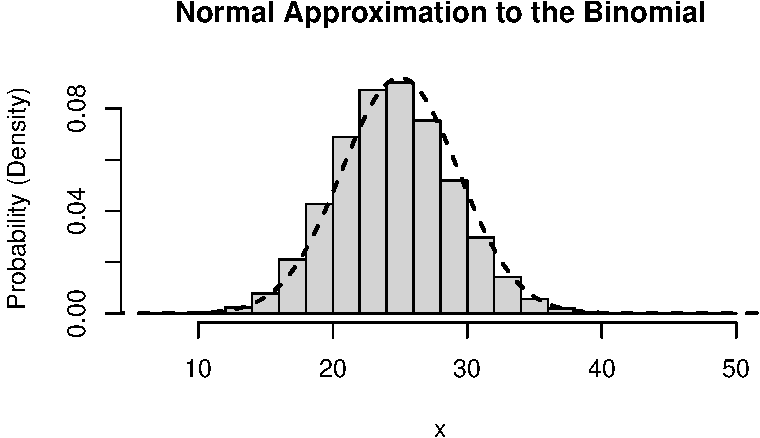
\includegraphics[keepaspectratio]{notes/chapter9_files/figure-pdf/fig-normal-approximation-1.pdf}}

}

\end{figure}%

One consideration that we need to make when applying this approximation
has to do with the fact that the normal distribution is continuous while
the binomial distribution is discrete. As a result, the normal
distribution can take on any value on the real line, where the binomial
is limited to the integers. A question that we must answer is what to do
with the non-integer valued numbers. The natural solution is to rely on
rounding. That is, for any value between \([1.5, 2.5)\) we would round
to the nearest integer, which is \(2\).

\begin{definition}[Continuity
Correction]\protect\hypertarget{def-continuity-correction}{}\label{def-continuity-correction}

The continuity correction is a technique for adjusting the probabilities
computed using a continuous approximation to a discrete random variable.
The correction relies on rounding non-integer values, which may be
observed with regards to the continuous random variable, to the
corresponding integer values for the discrete random variable that is
being approximated.

\end{definition}

This natural solution is in fact a fairly useful technique, and it is
the one that we will make use of in the normal approximation. While
rounding is quite natural, the process for leveraging this idea in
probability approximation is somewhat backwards. That is, we typically
will need to go from probabilities relating to \(X\) and transform those
into probabilities relating to \(W\). So, for instance, if we wish to
know \(P(X \leq 2)\), then we need to be able to make this a statement
regarding the random variable \(W\). In order to do this we need to ask
``what is the largest value for \(W\) that would get rounded to \(2\)?''
The answer is \(2.5\) and so \(P(X \leq 2) \approx P(W \leq 2.5)\).

A similar adjustment would be required if we instead wanted
\(P(X \geq 5)\). Here we would ask ``what is the smallest value for
\(W\) which would get rounded to \(5\)?'' and note that the answer is
\(4.5\). Thus, \(P(X \geq 5) \approx P(W \geq 4.5)\). Once we have
expressed the probability of interest in terms of the normal random
variable, we can use the standard techniques previously outlined to
compute the relevant probabilities. It is very important to note that
these two results are of the form \(X \geq x\) and \(X \leq x'\). If we
instead had considered \(X > x\) or \(X < x'\), we would need to take an
additional step.

For continuous random variables whether \(X \geq x\) or \(X > x\) is
considered makes no difference. However, for discrete random variables
this is not the case. As a result we should first convert the event the
an equivalent event which contains the equality sign within the
inequality, and then apply the continuity correction. That is, if we
want \(P(X > 3)\) first note that for \(X > 3\) to hold, we could
equivalently write this as \(X \geq 4\). Alternatively, if the event of
interest is \(X < 8\), this is the same as \(X \leq 7\).

\begin{example}[Charles and Sadie Payouts over a
Year]\protect\hypertarget{exm-normal-approximation}{}\label{exm-normal-approximation}

Charles and Sadie are back sitting at the coffee shop, reflecting on all
of the probability that they have learned since their games began. They
realize that each time they play the game to see who will pay, that is a
Bernoulli trial with \(0.5\) probability. As a result, over the course
of the year, if they go \(200\) times to get coffee, the number of times
each of them will have to pay is governed by a \(\text{Bin}(200, 0.5)\)
random variable. Charles realizes that this is infeasible to work with a
binomial distribution, and so seeks another way.\footnote{Note that, for
  instance,
  \(\binom{200}{75} = 168849997346404286704489530268603459022868706883102845056\).
  This is \(168\) septendecillion. This is \(3.2\) million times more
  than the number of possible arrangements of a chess board. This is a
  silly large number.} Sadie suggest that they could use the normal
approximation to the binomial.

\begin{enumerate}
\def\labelenumi{\alph{enumi}.}
\tightlist
\item
  What is the approximate probability that Charles pays more than
  \(115\) times in a year, expressed in terms of \(\Phi\).
\item
  What is the approximate probability that Sadie will pay between \(86\)
  and \(107\) times? Explain how this can be approximated numerically.
\item
  Give an upper and lower bound that both Charles and Sadie can be
  \(95\%\) sure they will pay between (that is, two numbers such that
  the probability they pay at least the lower and at most the upper
  bound is \(0.95\)).
\end{enumerate}

\begin{tcolorbox}[enhanced jigsaw, arc=.35mm, rightrule=.15mm, breakable, bottomrule=.15mm, left=2mm, toprule=.15mm, leftrule=.75mm, opacityback=0, colback=white, colframe=quarto-callout-color-frame]

\vspace{-3mm}\textbf{Solution}\vspace{3mm}

For these questions we will take \(X \sim \text{Bin}(200, 0.5)\), and
therefore, \(X \dot\sim W \sim N(100, 50)\). Thus, to calculate these
probabilities, we can use normal approximations, making sure to apply
the continuity corrections.

\begin{enumerate}
\def\labelenumi{\alph{enumi}.}
\tightlist
\item
  We want \(P(X > 115)\). This is the same as asking \(P(X \geq 116)\),
  and with the continuity correction,
  \(P(X \geq 116) \approx P(W \geq 115.5)\). Thus, we take
  \[P(W \geq 115.5) = P\left(Z \geq \frac{115.5 - 100}{\sqrt{50}}\right) = 1 - \Phi\left(2.192\right).\]
  This could be worked out using a normal probability
  calculator.\footnotemark{}
\item
  We want
  \[P(86 < X < 107) = P(87 \leq X \leq 106 \approx P(87.5 \leq W \leq 106.5).\]
  Note that if we consider
  \[\frac{106.5 - 100}{\sqrt{50}} = 0.919 \quad\text{and}\quad \frac{87.5 - 100}{\sqrt{50}} = -1.838.\]
  If we wanted to get a rough approximation of this, we could say that,
  from the empirical rule, the probability that
  \begin{multline*}P(\mu_W - 1.838\sigma_W \leq W \leq \mu_W + 0.919\sigma_W) \leq P(\mu_W - 2\sigma_W \leq W \leq \mu_W + \sigma_W) \\
  = \frac{0.68}{2} + \frac{0.95}{2} = 0.815.\end{multline*} Note that
  this gives an upper bound on the probability. We could also get a
  lower bound on the probability by moving in the other directions,
  \[P(\mu_W - 1.838\sigma_W \leq W \leq \mu_W + 0.919\sigma_W) \leq P(\mu_W - 2\sigma_W \leq W \leq \mu_W) = \frac{0.95}{2} = 0.475.\]
  This gives a fairly wide range, but we can be relatively confident it
  will be a lot closer to \(0.815\) than to \(0.475\), since the values
  are a lot close to \(-2\) and \(1\) than \(-1\) and
  \(0\).\footnotemark{}
\item
  Note that, if we use a normal approximation and the empirical rule, we
  know that there is approximately a \(0.95\) probability that a random
  variable falls within \(2\sigma\) of the mean. The mean of \(W\) is
  \(100\) and \(\sigma = \sqrt{50}\), so we can take the interval
  \([85.8578, 114.1421]\). Note that if we widen this slightly the
  probability will increase slightly, so that the probability
  \(W \in [85.5, 114.5]\) must be greater than \(0.95\). The quantity
  \(P(85.5 \leq W \leq 114.5)\) corresponds to
  \(P(86 \leq X \leq 114)\), and so we can say that Charles and Sadie
  can each be roughly \(95\%\) confident that they will need to pay
  between \(86\) and \(114\) times.\footnotemark{}
\end{enumerate}

\end{tcolorbox}

\footnotetext{Doing so results in 0.0141898. Note, if we had used a
binomial probability calculator instead, we would have gotten
0.0140627.}

\footnotetext{In fact, the actual probability here is 0.7824647.}

\footnotetext{The actual binomial probabilities here are 0.9519985,
while the normal approximation is 0.959695.}

\end{example}

When it is not necessary, it rarely makes sense to use an approximation.
There will be cases where the approximation is directly useful, and in
those moments it is great to be able to use it. This example of using
the normal distribution to approximate a discrete random variable serves
as a nice bridge from the study of probability to the study of
statistics. In statistics we take a different view of the types of
problems we have been considering to date, and we require the tools of
probability that have been brought forth. As a result, a deep comfort
with manipulating probability expressions is required to build a strong
foundation while studying statistics.

\section{\texorpdfstring{The \(t\)
Distribution}{The t Distribution}}\label{the-t-distribution}

The \(t\) distribution, or Student's \(t\) distribution named after the
individual who popularized the distribution,\footnote{William Gosset,
  was a statistician, chemist, and brewer who worked as the head brewer
  at Guinness. During his work there he was concerned with statistical
  problems related to testing the quality of ingredients. In this work,
  he made a discovery relating to the \(t\) distribution which was
  published in a scientific article under the pseudonym Student (hence,
  Student's \(t\) distribution). Guinness preferred that their employees
  used pseudonyms when publishing scientific articles, perhaps to ensure
  that trade secrets were kept secret, and hence Student's \(t\) was
  born.} is a bell-shaped distribution, not unlike the normal. It is
parameterized by a single parameter, typically denoted \(\nu\) and
referred to as the \textbf{degrees of freedom} of the distribution.

While it has a similar shape to the normal distribution, the \(t\)
distribution has \textbf{heavier tails} than the normal, which is to say
that the probability of observing an extreme event is larger in the
\(t\) than in the normal. The \(t\) distribution is always centered at
\(0\). Neither the probability density function nor the cumulative
distribution function are particularly nice,\footnote{The density
  function, for instance, is given by
  \[\frac{\Gamma(\frac{\nu+1}{2})}{\sqrt{\pi\nu}\Gamma(\frac{\nu}{2})}\left(1+\frac{x^2}{\nu}\right)^{-(\nu+1)/2},\]
  where \(\Gamma(\cdot)\) is the Gamma function, a mathematical
  expression touched on later.} however, the mean, median, and mode are
all \(0\). The variance of the \(t\) distribution is only properly
defined for \(\nu > 2\), and in this case if \(X \sim t_{\nu}\) then
\[\text{var}(X) = \frac{\nu}{\nu - 2}.\]

The parameter \(\nu\) is any real, positive number. Typically, \(\nu\)
is restricted to be a positive integer, for reasons that will become
clear later. As \(\nu\) increases, the tails of the \(t\) distribution
become smaller and smaller. In the limit, as \(\nu\) tends towards
\(\infty\), the \(t\) distribution approaches the standard normal. In
fact, when \(\nu \geq 30\), the two distributions are nearly identical.

\begin{figure}[H]

\caption{\label{fig-t-dist}The \(t\) distribution compared with the
standard normal. As the degrees of freedom increasing, the density
function for the \(t\) becomes closer and closer to the standard
normal's density function, and at \(\nu = \infty\) they theoretically
overlap.}

\centering{

\pandocbounded{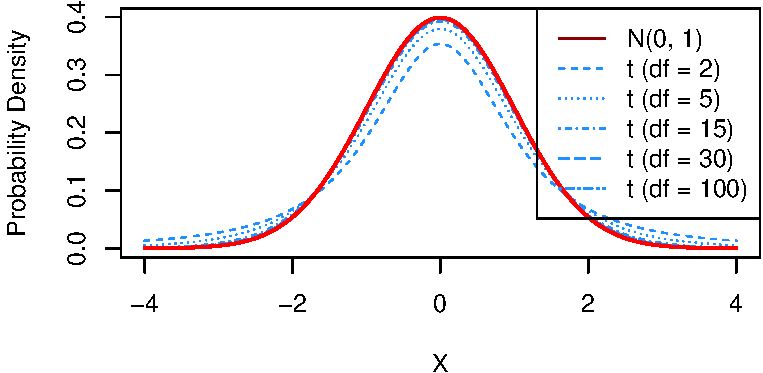
\includegraphics[keepaspectratio]{notes/chapter9_files/figure-pdf/fig-t-dist-1.pdf}}

}

\end{figure}%

Note that, compared with the normal distribution, the \(t\)
distributions (particularly with lower degrees of freedom) are more
likely to observe extreme events. Based on the empirical rule, we know
that the probability of observing an event outside of \(\pm 3\) on the
standard normal is \(0.3\%\). This is incredibly rare. By contrast, a
\(t\) distribution with \(2\) degrees of freedom has a 9.55\% chance of
observing a value outside of the interval \(\pm 3\). When it is said
that the \(t\) distribution has heavier tails, this is what is meant.

\begin{example}[Characterizing Scale
Errors]\protect\hypertarget{exm-t-distribution}{}\label{exm-t-distribution}

Charles and Sadie have been using a new kitchen scale to weigh the
vegetables that they have started to grow in their garden. They are
trying to keep a detailed log of the counts and weights of all the
vegetables that they harvest so that they may know what works and what
does not. Unfortunately, they realize that the scale that they are using
is not perfectly accurate and seems to be introducing random errors.
They begin to investigate these errors.

\begin{enumerate}
\def\labelenumi{\alph{enumi}.}
\tightlist
\item
  Suppose that, by repeatedly weighing a reference weight, they
  determine that the mean error is equal to \(0\) and the variance is
  equal to \(1\). If the errors are normally distributed, approximately
  how likely is it that Sadie and Charles observe an error that is
  greater than \(2\) grams?
\item
  Sadie and Charles are skeptical of the normality of the errors. They
  suspect that perhaps the variance they measured was incorrect, and
  should have actually been \(2\). If this is the case, what is the
  corresponding \(t\) distribution that would be valid?
\item
  If the errors truly follow the \(t\) distribution from part (b), is it
  more or less likely that Sadie and Charles will observe an error
  greater than \(2\) grams, compared with (a)? Explain.
\end{enumerate}

\begin{tcolorbox}[enhanced jigsaw, arc=.35mm, rightrule=.15mm, breakable, bottomrule=.15mm, left=2mm, toprule=.15mm, leftrule=.75mm, opacityback=0, colback=white, colframe=quarto-callout-color-frame]

\vspace{-3mm}\textbf{Solution}\vspace{3mm}

\begin{enumerate}
\def\labelenumi{\alph{enumi}.}
\item
  Given their findings this will follow a \(N(0, 1)\) distribution. By
  the empirical rule, we know that approximately \(95\%\) of
  observations will fall within \(\pm 2\) standard deviations of the
  mean, which in this case is \(1\) gram. Thus, they should observe
  errors that are smaller than \(2\) in magnitude \(95\%\) of the time,
  which means the probability of observing an error larger than this is
  approximately \(0.05\).
\item
  If instead they are faced with a \(t\) distribution, if the variance
  \(2\), then the number of degrees of freedom can be solved for by
  taking \[2 = \frac{\nu}{\nu - 2} \implies \nu = 4.\] As a result,
  based on their measured results this would suggest a \(t_4\)
  distribution.
\item
  If the true error distribution is \(t_4\), then it is more likely to
  observe extreme values since the tails of the \(t\) distribution are
  heavier than the tails of the normal distribution. Using the computer
  to estimate this probability gives 0.1161, which is quite a lot larger
  than the \(0.05\) from (a).
\end{enumerate}

\end{tcolorbox}

\end{example}

The \(t\) distribution, with its close connections to the normal
distribution, will often arise in statistical applications. While less
central than the normal, the \(t\) distribution is nevertheless very
important for statistical analyses, and will be explored in more depth
in the second part of these notes.

\section{The Exponential
Distribution}\label{the-exponential-distribution}

The exponential distribution is a single-parameter, skewed distribution
that is always positive. The distribution has a probability density
functioned supported on \([0,\infty)\), which exhibits exponential decay
over this interval, meaning that extreme events are possible, but fairly
unlikely. The probability density function is characterized by a single
parameter referred to as the rate, and is typically denoted using
\(\lambda\). Thus, if \(X \sim \text{Exp}(\lambda)\), then \(X\) is a
continuous random variable with probability density function given by
\[f(x) = \lambda\exp(-\lambda x), \ x \in [0,\infty).\] The cumulative
distribution function for the exponential can be obtained through
integration of the density, resulting in
\[F(x) = 1 - \exp(-\lambda x).\] Moreover, if
\(X \sim \text{Exp}(\lambda)\), then \(E[X] = \dfrac{1}{\lambda}\) and
\(\text{var}(X) = \dfrac{1}{\lambda^2}\).\footnote{Note, some authors
  instead parameterize the exponential distribution with the mean,
  \(\mu\). In this case, \(E[X] = \mu\), \(\text{var}(X) = \mu^2\), but
  the density will have \(\dfrac{1}{\mu}\) in place of \(\lambda\).}

\begin{figure}[H]

\caption{\label{fig-exp-dist}The exponential distribution shown for
decreasing values of \(\lambda\). Note that as the rate decreases, the
mean increases. As a result, at this resolution, the curve will appear
to flatten out. This has the effect of making larger events increasing
likely, while decreasing the relative likelihood of small events.}

\centering{

\pandocbounded{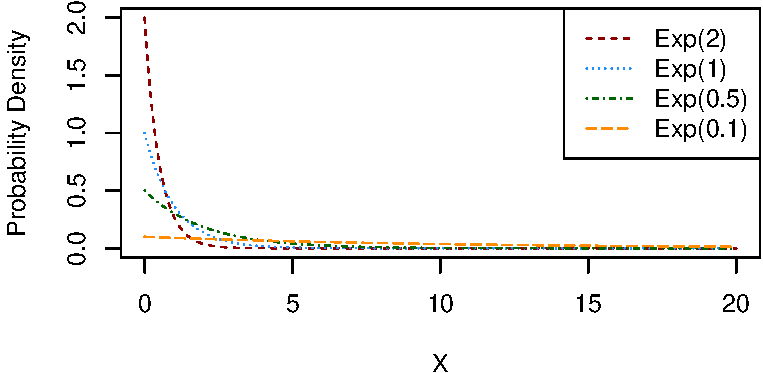
\includegraphics[keepaspectratio]{notes/chapter9_files/figure-pdf/fig-exp-dist-1.pdf}}

}

\end{figure}%

\begin{example}[Charles and Sadie Install Solar
Panels]\protect\hypertarget{exm-lifespan-of-solar-panels}{}\label{exm-lifespan-of-solar-panels}

Charles and Sadie are considering purchasing solar panels for a plot of
land they wish to develop. The manufacturer of the solar panels suggests
that the panels are exponentially distributed with a mean lifetime of 15
years.

\begin{enumerate}
\def\labelenumi{\alph{enumi}.}
\tightlist
\item
  What is the variance in the expected lifetime of these panels?
\item
  What is the probability that the panels will need to be replaced in
  less than \(10\) years?
\item
  What is the probability that the panels last at least \(20\) years
  before needing to be replaced?
\end{enumerate}

\begin{tcolorbox}[enhanced jigsaw, arc=.35mm, rightrule=.15mm, breakable, bottomrule=.15mm, left=2mm, toprule=.15mm, leftrule=.75mm, opacityback=0, colback=white, colframe=quarto-callout-color-frame]

\vspace{-3mm}\textbf{Solution}\vspace{3mm}

\begin{enumerate}
\def\labelenumi{\alph{enumi}.}
\tightlist
\item
  The mean lifespan is \(15\) and so we must have that
  \(\lambda = \dfrac{1}{15}\). Thus,
  \(X \sim \text{Exp}(\dfrac{1}{15})\), and
  \(\text{var}(X) = \dfrac{1}{225}\).
\item
  This is
  \[P(X \leq 10) = F(10) = 1 - \exp(-\dfrac{10}{15}) =  1 - \exp(-2/3) \approx 0.48658.\]
\item
  This is
  \[P(X \geq 20) = 1 - F(20) = 1 - (1 - \exp(-\dfrac{20}{15})) = \exp(-4/3) \approx 0.26360.\]
\end{enumerate}

\end{tcolorbox}

\end{example}

\subsection{The Memoryless Property of the Exponential
Distribution}\label{the-memoryless-property-of-the-exponential-distribution}

The exponential distribution has one particularly important property
that makes it a mathematically convenient model, while often challenging
its validity for real-world applications. Specifically, the exponential
distribution exhibits a \textbf{memoryless} property.\footnote{The
  exponential distribution shares this property with the geometric
  distribution, and can as such be thought of as a continuous analog to
  the geometric distribution.} The memoryless property states, roughly,
that if you observe a process that is exponentially distributed before
an event has been observed, the remaining time until an event will by
exponentially distributed with the same parameter, with the current time
being counted as zero. That is, the process seems to not have any memory
of the elapsed duration.

\begin{tcolorbox}[enhanced jigsaw, arc=.35mm, title={The Memoryless Property of an Exponential}, rightrule=.15mm, coltitle=black, opacitybacktitle=0.6, colbacktitle=quarto-callout-tip-color!10!white, leftrule=.75mm, colback=white, breakable, titlerule=0mm, toptitle=1mm, bottomtitle=1mm, bottomrule=.15mm, toprule=.15mm, opacityback=0, left=2mm, colframe=quarto-callout-tip-color-frame]

Suppose that \(X \sim \text{Exp}(\lambda)\). Then, for any real numbers
\(t \geq s \geq 0\), \[P(X \geq t | X \geq s) = P(X \geq t - s).\] In
this way, the elapsed time does not impact future probabilities, as the
process ``forgets''.

\end{tcolorbox}

Suppose that the lifespan of an electrical component is thought to be
exponentially distributed with parameter \(\lambda\). Then, we could
work out the probability that the component lasts at least \(10\) years
to be \(1 - F(10) = \exp(-10\lambda)\). However, suppose that we knew
that the component had already been in service for \(8\) years. Given
this information, we can conclude that the probability that the
component will last another \(10\) years, is
\[P(X \geq 18 | X \geq 8) = P(X \geq 18-8) = P(X \geq 10) = \exp(-10\lambda).\]
Thus, if we know the component has been in service for \(10\) years and
is still functioning, then it will be equally likely that it will last
to \(18\) years as it was to have lasted to \(10\) from the start.

\begin{tcolorbox}[enhanced jigsaw, arc=.35mm, title={Proof of the Memoryless Property}, rightrule=.15mm, coltitle=black, opacitybacktitle=0.6, colbacktitle=quarto-callout-warning-color!10!white, leftrule=.75mm, colback=white, breakable, titlerule=0mm, toptitle=1mm, bottomtitle=1mm, bottomrule=.15mm, toprule=.15mm, opacityback=0, left=2mm, colframe=quarto-callout-warning-color-frame]

Note that the memoryless property can be proved using our standard
notions of joint and conditional probabilities. Specifically, suppose
that \(X \sim \text{Exp}(\lambda)\), and take the event \(A\) to be
\(\{ X \geq t \}\) and the event \(B\) to be \(\{X \geq s \}\), for
\(t \geq s\). Thus, if \(A\) occurs then we know that \(B\) also occurs,
since \(t \geq s\), and as such we have that
\(A\cap B = A = \{X \geq t\}\). Thus, \begin{align*}
P(X \geq t | X \geq s) &= \frac{P(A \cap B)}{P(B)} \\
&= \frac{P(A)}{P(B)} \\
&= \frac{\exp(-t\lambda)}{\exp(-s\lambda)} \\
&= \exp(-(t-s)\lambda) \\
&= P(X \geq t - s).
\end{align*}

\end{tcolorbox}

\begin{example}[Charles and Sadie Consider Used Solar
Panels]\protect\hypertarget{exm-lifespan-of-solar-panels}{}\label{exm-lifespan-of-solar-panels}

Charles and Sadie, in doing research on solar panels, are considering
going the route of purchasing used solar panels instead of the new ones.
The two options in front of them are to go with the new solar panels
with a mean lifetime of \(15\) years, or purchase the used panels
instead. When they were manufactured, the panels had an anticipated
lifespan of \(18\) years, but they have been in service (and are still
functioning) for a total of \(12\) years so far.

\begin{enumerate}
\def\labelenumi{\alph{enumi}.}
\tightlist
\item
  Which is more likely: that the new solar panels will last \(15\) years
  or that the used solar panels will last to a total of \(27\) years,
  given the current status?
\item
  Is the exponential distribution likely to be reasonable for this
  setting? Explain.
\end{enumerate}

\begin{tcolorbox}[enhanced jigsaw, arc=.35mm, rightrule=.15mm, breakable, bottomrule=.15mm, left=2mm, toprule=.15mm, leftrule=.75mm, opacityback=0, colback=white, colframe=quarto-callout-color-frame]

\vspace{-3mm}\textbf{Solution}\vspace{3mm}

\begin{enumerate}
\def\labelenumi{\alph{enumi}.}
\tightlist
\item
  We know that
  \(P(X \geq 15) = 1 - F(15) = 1 - (1 - \exp(-15/15)) = \exp(-1)\).
  Thus, there is a probability of approximately \(0.3679\) that the new
  panels will last for \(15\) years. Using the memoryless property we
  can work out the probability for the used panels.
  \[P(X' \geq 27 | X' \geq 12) = P(X' \geq 27-12) = P(X' \geq 15).\]
  Since the used panels have a mean of \(18\), the rate will be
  \(\dfrac{1}{18}\), and so the probability is
  \(\exp(-\dfrac{15}{18}) \approx 0.4346\). Thus, it is more likely that
  the used panels survive to \(27\) than the new panels surviving to
  \(15\), given that we have observed the new panels functioning at
  \(12\) years.
\item
  The exponential distribution is likely not appropriate in this case,
  owing to the memoryless property. Specifically, it seems unlikely that
  a panel that has been in use for \(15\) years will continue
  functioning for an additional \(15\) years with the same probability
  as it was to hit \(15\) years in the first place. We know that as
  panels are in use, they are likely suffering ongoing deterioration
  from exposure, just simply through use.
\end{enumerate}

\end{tcolorbox}

\end{example}

\subsection{The Exponential Distribution and Poisson
Processes}\label{the-exponential-distribution-and-poisson-processes}

The exponential distribution is closely related to the Poisson
distribution through the Poisson process (recall
Section~\ref{sec-poisson-process} for the definition of the Poisson
process). In particular, recall that in a Poisson process we are
counting the number of events that occur over a particular interval. We
concluded that the number of events, under the assumptions of the
Poisson process, that occur during a set interval will follow a
particular Poisson distribution. The exponential distribution arises in
this context as the distribution for the \textbf{interarrival times}.
That is, the number of events that occur during an interval will follow
a Poisson distribution, however, the time between any two consecutive
events will follow an exponential distribution, with the same rate
parameter.

\begin{tcolorbox}[enhanced jigsaw, arc=.35mm, title={The Interarrival Times for a Poisson Process}, rightrule=.15mm, coltitle=black, opacitybacktitle=0.6, colbacktitle=quarto-callout-tip-color!10!white, leftrule=.75mm, colback=white, breakable, titlerule=0mm, toptitle=1mm, bottomtitle=1mm, bottomrule=.15mm, toprule=.15mm, opacityback=0, left=2mm, colframe=quarto-callout-tip-color-frame]

Suppose that \(X\) follows a Poisson process with rate \(\alpha\). Then
the time between any two successive events will be distributed according
to a \(\text{Exp}(\alpha)\) distribution.

\end{tcolorbox}

\begin{example}[Sadie's Vegan Bakery Aspirations:
Revisited]\protect\hypertarget{exm-exp-poi-process}{}\label{exm-exp-poi-process}

Sadie has continued to consider the prospect of opening up a vegan
bakery. Market research continues to suggest that it is expected that
\(168\) customers would arrive per week, supposing that Sadie's bakery
was open \(8\) hours a day, \(7\) days a week.

\begin{enumerate}
\def\labelenumi{\alph{enumi}.}
\tightlist
\item
  How long (in hours) should Sadie expect to wait before the first
  customer arrives?
\item
  How long (in hours) should Sadie expect to wait between the 99th and
  100th customer arrivals?
\item
  Suppose that Sadie was having a particularly slow start to the day,
  and it had been \(45\) minutes with no customers. What is the
  probability Sadie has to wait at least another \(15\) minutes before
  one finally arrives?
\end{enumerate}

\begin{tcolorbox}[enhanced jigsaw, arc=.35mm, rightrule=.15mm, breakable, bottomrule=.15mm, left=2mm, toprule=.15mm, leftrule=.75mm, opacityback=0, colback=white, colframe=quarto-callout-color-frame]

\vspace{-3mm}\textbf{Solution}\vspace{3mm}

\begin{enumerate}
\def\labelenumi{\alph{enumi}.}
\tightlist
\item
  Customers arrive at a rate of \(3\) per hour, and thus, the time
  between any customers arriving will be distributed as an
  \(\text{Exp}(3)\) random variable. As a result, Sadie should expect to
  wait \(\dfrac{1}{3}\) hours (or \(20\) minutes) for the first
  customer.
\item
  Because all interarrival times are distributed the same way, the time
  between the \(99\)th and \(100\)th customer is distributed exactly as
  the time between the \(0\)th and \(1\)st, and as a result, the answer
  is the same as part (a).
\item
  Let \(T\) be the time of arrival for the first customer. We want to
  know \(P(T > 1 | T > \dfrac{3}{4})\) which we can solve for knowing
  that \(T \sim \text{Exp}(3)\) and as such the memoryless property
  applies. Thus,
  \[P(T > 1 | T > \dfrac{3}{4}) = P(T > \dfrac{1}{4}) = 1 - (1 - \exp(-\dfrac{3}{4})) = \exp(-3/4) \approx 0.4724.\]
\end{enumerate}

\end{tcolorbox}

\end{example}

\subsection{The Exponential Distribution in the
Real-World}\label{the-exponential-distribution-in-the-real-world}

The exponential distribution arises frequently in the modelling of
extreme events and in the lifetimes of objects. Most frequently, it
arises as the interarrival time in Poisson processes. While it is often
not a perfect representation of the underlying reality, it will
frequently work well enough to provide useful results. The exponential
distribution is itself a part of a large family of distributions know as
the gamma distribution. We will consider the Gamma distribution next,
however, owing to the compact form and the frequent use of the
exponential distribution, it is worth considering separate from the
remainder of the gamma family distributions.

\section{\texorpdfstring{\(\int\) The Gamma
Distribution}{\textbackslash int The Gamma Distribution}}\label{int-the-gamma-distribution}

The Gamma distribution is a two-parameter distribution, supported on
\([0,\infty)\). The distributions parameters are typically denoted
\(\alpha\) and \(\beta\) and are referred to as the \textbf{shape} and
\textbf{scale} parameter, respectively. The probability density function
for \(X \sim \text{Gamma}(\alpha, \beta)\) is given by
\[f(x) = \frac{1}{\Gamma(\alpha)\beta^{\alpha}}x^{\alpha - 1}\exp(-\frac{x}{\beta}).\]
In this expression, \(\Gamma(\alpha)\) is the \textbf{Gamma function}, a
function which is expressible in general only via an integral.

\begin{definition}[Gamma
Function]\protect\hypertarget{def-gamma-function}{}\label{def-gamma-function}

The Gamma function, denoted \(\Gamma(k)\), is a function given by
\[\Gamma(k) = \int_{0}^\infty x^{k-1}e^{-x}dx.\] If \(k\) is a positive
integer, then \(\Gamma(k) = (k-1)!\), and in general,
\(\Gamma(k) = (k-1)\Gamma(k - 1)\).

\end{definition}

Note that if \(X \sim \text{Gamma}(\alpha, \beta)\), then
\(E[X] = \alpha\beta\) and \(\text{var}(X) = \alpha\beta^2\).\footnote{As
  is the case with many distributions, some authors will use a different
  parametrization of the Gamma distribution. In particular, they may use
  parameters that equal \(\alpha\) and then \(1/\beta\), making the
  necessary substitutions in the different quantities.} The cumulative
distribution function can be expressed as
\[F(x) = \frac{1}{\Gamma(\alpha)}\gamma(\alpha, \frac{x}{\beta}),\]
where \(\gamma(a, b)\) is the lower incomplete gamma function, given by
\[\gamma(a, b) = \int_{0}^b x^{a-1}e^{-x}dx.\]

\begin{figure}[H]

\caption{\label{fig-gamma-dist}The Gamma distribution shown for various
combinations of \(\alpha\) and \(\beta\).}

\centering{

\pandocbounded{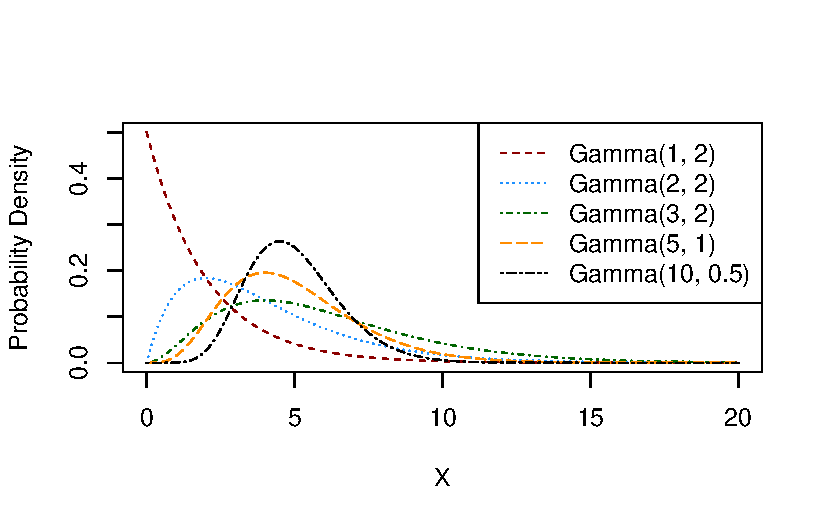
\includegraphics[keepaspectratio]{notes/chapter9_files/figure-pdf/fig-gamma-dist-1.pdf}}

}

\end{figure}%

\subsection{Connection to Other
Distributions}\label{connection-to-other-distributions}

It was briefly mentioned above that the exponential distribution is
actually a special case of the Gamma distribution. If we investigate the
corresponding desnity functions we may note that taking \(\alpha = 1\)
and \(\beta = \dfrac{1}{\lambda}\) gives us
\[f(x) = \lambda\exp(-\lambda x),\] which is exactly the exponential
probability density function. As a result we can say that
\(\text{Exp}(\lambda) = \text{Gamma}(1, 1/\lambda)\). The Gamma
distribution is connected to several important distributions that arise
throughout the study of probability and statistics.

Beyond the exponential, the most prominent distribution which is
connecte to the Gamma is the chi-squared distribution. The chi-squared
distribution is a distribution that arises in many statistical inference
procedures. It is characterized by a single parameter, \(\nu\), referred
to as the degrees of freedom. To characterize the chi-squared
distribution with \(\nu\) degrees of freedom, denoted \(\chi^2_\nu\), we
take \(X \sim \text{Gamma}(\nu/2, 2)\). Thus, the mean of the
distribution is \(\nu\) and the variance is \(2\nu\).

\begin{figure}[H]

\caption{\label{fig-chisq-dist}The chi-sqaured distribution shown for
increasing degrees of freedom.}

\centering{

\pandocbounded{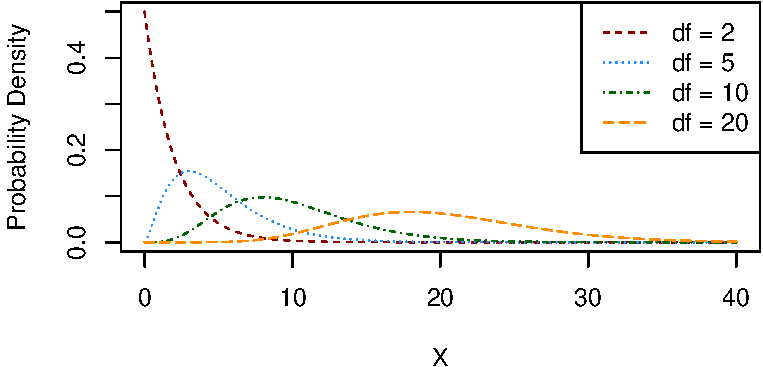
\includegraphics[keepaspectratio]{notes/chapter9_files/figure-pdf/fig-chisq-dist-1.pdf}}

}

\end{figure}%

\section{Continuous Probability Calculations in
R}\label{sec-r-continuous}

Just as with the named discrete distributions, R provides functions for
calculating probabilities related to continuous random variables. The
relevant functions are, as in the discrete case, \texttt{d\{distname\}}
and \texttt{p\{distname\}}, where \texttt{\{distname\}} is one the named
distributions. These evaluate the density and cumulative distribution
functions, respectively. So for instance, \texttt{dnorm} and
\texttt{pnorm} calculate normal probabilities, \texttt{dt} and
\texttt{pt} calculate probability for the \(t\) distribution,
\texttt{dexp} and \texttt{pexp} calculate exponential probabilities,
\texttt{dgamma} and \texttt{pgamma} calculate Gamma probabilities, and
\texttt{dchisq} and \texttt{pchisq} calculate the chi-squared
probabilities.

Each function takes in a set of parameters to indicate which of the
specific distributions is being considered. Note, it is important to
ensure that the correct parameterizations are used. For the normal, the
functions can take arguments for the mean and standard
deviation\footnote{Recall, the standard deviation is the square root of
  the variance.} of the normal. If not provided, it will default to the
standard normal. The \(t\) and chi-squared distributions each take a
degrees of freedom argument, named \texttt{df}. For the exponential, the
parameter is named \texttt{rate}. The Gamma distribution can be
parameterized either as the shape/scale, or the shape/rate
characterization, where we learned the former.

\begin{Shaded}
\begin{Highlighting}[]
\DocumentationTok{\#\# Normality}
\CommentTok{\# N(0, 1)}
\FunctionTok{dnorm}\NormalTok{(}\FloatTok{0.25}\NormalTok{) }\CommentTok{\# f(0.25)}
\FunctionTok{pnorm}\NormalTok{(}\FloatTok{0.25}\NormalTok{) }\CommentTok{\# P(X \textless{}= 0.25)}

\CommentTok{\# N(5, 4)}
\FunctionTok{dnorm}\NormalTok{(}\FloatTok{4.9}\NormalTok{, }\AttributeTok{mean =} \DecValTok{5}\NormalTok{, }\AttributeTok{sd =} \FunctionTok{sqrt}\NormalTok{(}\DecValTok{4}\NormalTok{)) }\CommentTok{\# f(4.9)}
\FunctionTok{pnorm}\NormalTok{(}\FloatTok{4.9}\NormalTok{, }\AttributeTok{mean =} \DecValTok{5}\NormalTok{, }\AttributeTok{sd =} \FunctionTok{sqrt}\NormalTok{(}\DecValTok{4}\NormalTok{)) }\CommentTok{\# P(X \textless{}= 4.9)}

\CommentTok{\# N(0, 1) {-} Explicitly}
\FunctionTok{dnorm}\NormalTok{(}\DecValTok{1}\NormalTok{, }\AttributeTok{mean =} \DecValTok{0}\NormalTok{, }\AttributeTok{sd =} \DecValTok{1}\NormalTok{) }\CommentTok{\# f(1)}
\FunctionTok{pnorm}\NormalTok{(}\DecValTok{1}\NormalTok{, }\AttributeTok{mean =} \DecValTok{0}\NormalTok{, }\AttributeTok{sd =} \DecValTok{1}\NormalTok{) }\CommentTok{\# P(X \textless{}= 1)}

\DocumentationTok{\#\# t{-}Distribution}
\CommentTok{\# t\_5}
\FunctionTok{dt}\NormalTok{(}\FloatTok{0.25}\NormalTok{, }\AttributeTok{df =} \DecValTok{5}\NormalTok{)}
\FunctionTok{pt}\NormalTok{(}\FloatTok{0.25}\NormalTok{, }\AttributeTok{df =} \DecValTok{5}\NormalTok{)}

\CommentTok{\# Consider the approach to the normal distribution}
\ControlFlowTok{for}\NormalTok{(df }\ControlFlowTok{in} \DecValTok{2}\SpecialCharTok{:}\DecValTok{30}\NormalTok{) \{}
  \FunctionTok{print}\NormalTok{(}\FunctionTok{paste0}\NormalTok{(}\StringTok{"The difference at df="}\NormalTok{, df, }\StringTok{" is "}\NormalTok{, }
                \FunctionTok{dt}\NormalTok{(}\DecValTok{0}\NormalTok{, }\AttributeTok{df=}\NormalTok{df) }\SpecialCharTok{{-}} \FunctionTok{dnorm}\NormalTok{(}\DecValTok{0}\NormalTok{)))}
\NormalTok{\}}

\DocumentationTok{\#\# Exponential Distribution}
\FunctionTok{dexp}\NormalTok{(}\DecValTok{2}\NormalTok{, }\AttributeTok{rate =} \DecValTok{1}\SpecialCharTok{/}\DecValTok{2}\NormalTok{)}
\FunctionTok{pexp}\NormalTok{(}\DecValTok{2}\NormalTok{, }\AttributeTok{rate =} \DecValTok{1}\SpecialCharTok{/}\DecValTok{2}\NormalTok{)}

\DocumentationTok{\#\# Gamma Distribution}
\FunctionTok{dgamma}\NormalTok{(}\DecValTok{2}\NormalTok{, }\AttributeTok{shape =} \DecValTok{1}\NormalTok{, }\AttributeTok{scale =} \DecValTok{2}\NormalTok{) }\CommentTok{\# Exp(2)}
\FunctionTok{pgamma}\NormalTok{(}\DecValTok{2}\NormalTok{, }\AttributeTok{shape =} \DecValTok{1}\NormalTok{, }\AttributeTok{scale =} \DecValTok{2}\NormalTok{) }\CommentTok{\# Exp(2)}

\DocumentationTok{\#\# Chisquare Distribution}
\FunctionTok{dchisq}\NormalTok{(}\DecValTok{2}\NormalTok{, }\AttributeTok{df =} \DecValTok{5}\NormalTok{)}
\FunctionTok{pchisq}\NormalTok{(}\DecValTok{2}\NormalTok{, }\AttributeTok{df =} \DecValTok{5}\NormalTok{)}

\CommentTok{\# Using Gamma Functions}
\FunctionTok{dgamma}\NormalTok{(}\DecValTok{2}\NormalTok{, }\AttributeTok{shape =} \DecValTok{5}\SpecialCharTok{/}\DecValTok{2}\NormalTok{, }\AttributeTok{scale =} \DecValTok{2}\NormalTok{)}
\FunctionTok{pgamma}\NormalTok{(}\DecValTok{2}\NormalTok{, }\AttributeTok{shape =} \DecValTok{5}\SpecialCharTok{/}\DecValTok{2}\NormalTok{, }\AttributeTok{scale =} \DecValTok{2}\NormalTok{)}

\DocumentationTok{\#\# [1] 0.3866681}
\DocumentationTok{\#\# [1] 0.5987063}
\DocumentationTok{\#\# [1] 0.199222}
\DocumentationTok{\#\# [1] 0.4800612}
\DocumentationTok{\#\# [1] 0.2419707}
\DocumentationTok{\#\# [1] 0.8413447}
\DocumentationTok{\#\# [1] 0.36572}
\DocumentationTok{\#\# [1] 0.5937329}
\DocumentationTok{\#\# [1] "The difference at df=2 is {-}0.0453888898081589"}
\DocumentationTok{\#\# [1] "The difference at df=3 is {-}0.0313896834535713"}
\DocumentationTok{\#\# [1] "The difference at df=4 is {-}0.0239422804014327"}
\DocumentationTok{\#\# [1] "The difference at df=5 is {-}0.0193355905789382"}
\DocumentationTok{\#\# [1] "The difference at df=6 is {-}0.0162095080915611"}
\DocumentationTok{\#\# [1] "The difference at df=7 is {-}0.0139508295691653"}
\DocumentationTok{\#\# [1] "The difference at df=8 is {-}0.0122432594400395"}
\DocumentationTok{\#\# [1] "The difference at df=9 is {-}0.0109073715297641"}
\DocumentationTok{\#\# [1] "The difference at df=10 is {-}0.00983389643540161"}
\DocumentationTok{\#\# [1] "The difference at df=11 is {-}0.00895252334474339"}
\DocumentationTok{\#\# [1] "The difference at df=12 is {-}0.00821597517837541"}
\DocumentationTok{\#\# [1] "The difference at df=13 is {-}0.00759129841351724"}
\DocumentationTok{\#\# [1] "The difference at df=14 is {-}0.00705482460894713"}
\DocumentationTok{\#\# [1] "The difference at df=15 is {-}0.00658911756135444"}
\DocumentationTok{\#\# [1] "The difference at df=16 is {-}0.0061810499326827"}
\DocumentationTok{\#\# [1] "The difference at df=17 is {-}0.00582055039416196"}
\DocumentationTok{\#\# [1] "The difference at df=18 is {-}0.00549976367829647"}
\DocumentationTok{\#\# [1] "The difference at df=19 is {-}0.00521247310882905"}
\DocumentationTok{\#\# [1] "The difference at df=20 is {-}0.00495369469000007"}
\DocumentationTok{\#\# [1] "The difference at df=21 is {-}0.00471938611875367"}
\DocumentationTok{\#\# [1] "The difference at df=22 is {-}0.00450623448251958"}
\DocumentationTok{\#\# [1] "The difference at df=23 is {-}0.00431149889709365"}
\DocumentationTok{\#\# [1] "The difference at df=24 is {-}0.00413289218794199"}
\DocumentationTok{\#\# [1] "The difference at df=25 is {-}0.00396849076497147"}
\DocumentationTok{\#\# [1] "The difference at df=26 is {-}0.00381666515429396"}
\DocumentationTok{\#\# [1] "The difference at df=27 is {-}0.00367602586770638"}
\DocumentationTok{\#\# [1] "The difference at df=28 is {-}0.00354538080016037"}
\DocumentationTok{\#\# [1] "The difference at df=29 is {-}0.0034237013897046"}
\DocumentationTok{\#\# [1] "The difference at df=30 is {-}0.00331009550733491"}
\DocumentationTok{\#\# [1] 0.1839397}
\DocumentationTok{\#\# [1] 0.6321206}
\DocumentationTok{\#\# [1] 0.1839397}
\DocumentationTok{\#\# [1] 0.6321206}
\DocumentationTok{\#\# [1] 0.1383692}
\DocumentationTok{\#\# [1] 0.150855}
\DocumentationTok{\#\# [1] 0.1383692}
\DocumentationTok{\#\# [1] 0.150855}
\end{Highlighting}
\end{Shaded}

\section*{Exercises}\label{exercises-7}
\addcontentsline{toc}{section}{Exercises}

\markright{Exercises}

\begin{exercise}[]\protect\hypertarget{exr-9.1}{}\label{exr-9.1}

A boy is trying to climb a slippery pole and finds that he can climb to
a height of at least \(1.850\) m once in \(5\) attempts, and to a height
of at least \(1.700\) m nine times out of ten. Assuming that the heights
he reaches form a normal distribution:

\begin{enumerate}
\def\labelenumi{\alph{enumi}.}
\tightlist
\item
  What is the mean and standard deviation of the distribution?
\item
  If he climbs the pole \(1000\) times, what height can he expect to
  exceed once? Express your answer in terms of \(\Phi(z)\).
\end{enumerate}

\end{exercise}

\begin{exercise}[]\protect\hypertarget{exr-9.2}{}\label{exr-9.2}

A machine produces widgets of which an average of \(10\%\) are
defective.

\begin{enumerate}
\def\labelenumi{\alph{enumi}.}
\tightlist
\item
  Find an approximate value for the probability that a random sample of
  \(500\) of these articles contains more than \(25\) which are
  defective.
\item
  What, approximately, is the probability that the sample contains fewer
  than \(60\) defectives?
\end{enumerate}

\end{exercise}

\begin{exercise}[]\protect\hypertarget{exr-9.3}{}\label{exr-9.3}

The mean inside diameter of a sample of \(200\) washers produced by a
machine is \(0.502\) inches with a standard deviation of \(0.005\)
inches. The purpose for which these washers are intended allows for a
maximum tolerance in the diameter of \(0.496\) to \(0.508\). If we
assume that the washer diameters are normally distributed, what is the
probability that a washer is defective?

\end{exercise}

\begin{exercise}[]\protect\hypertarget{exr-9.4}{}\label{exr-9.4}

The wingspans of the females of a certain species of bird of prey form a
normal distribution with mean \(168.75\)cm and a standard deviation of
\(6.5\)cm. The wingspans of males of the species are normally
distributed with mean \(162.5\) and standard deviation of \(6\). What is
the probability if, with a male and female selected at random, the male
has the longer wingspan?

\end{exercise}

\begin{exercise}[]\protect\hypertarget{exr-9.5}{}\label{exr-9.5}

~

\begin{enumerate}
\def\labelenumi{\alph{enumi}.}
\tightlist
\item
  Find the probability of getting between \(3\) and \(6\) heads
  inclusive in \(10\) tosses of a fair coin.
\item
  Approximate the same probability using the normal approximation. How
  close is the approximation?
\end{enumerate}

\end{exercise}

\begin{exercise}[]\protect\hypertarget{exr-9.6}{}\label{exr-9.6}

Suppose that the cumulative distribution function of \(T\) is
\[F(t) = 1 - e^{-0.45t}.\]

\begin{enumerate}
\def\labelenumi{\alph{enumi}.}
\tightlist
\item
  Find \(P(T > 3)\).
\item
  Find the median of \(T\).
\end{enumerate}

\end{exercise}

\begin{exercise}[]\protect\hypertarget{exr-9.7}{}\label{exr-9.7}

Suppose that for a random variable, \(X\),
\[F(x) = \frac{x(x^2 + 9x + 27)}{(x+3)^3}.\]

\begin{enumerate}
\def\labelenumi{\alph{enumi}.}
\tightlist
\item
  What is the probability \(X\) falls between \(1\) and \(3\)?
\item
  What is the median of \(X\)?
\item
  What is \(\zeta(0.3)\) for \(X\)?
\end{enumerate}

\end{exercise}

\begin{exercise}[]\protect\hypertarget{exr-9.8}{}\label{exr-9.8}

Resistors labeled \(100\Omega\) have true resistances that uniformly
fall between \(80\Omega\) and \(120\Omega\). Let \(X\) be the mass of a
randomly chosen resistor.

\begin{enumerate}
\def\labelenumi{\alph{enumi}.}
\tightlist
\item
  What is the probability that a resistor has resistance equal to
  \(90\Omega\).
\item
  What proportion of resistors have resistance less than \(90\Omega\)?
\item
  Find the mean resistance.
\item
  Find the variance of the resistances.
\item
  Find the probability that the resistance is less than \(k\Omega\), for
  arbitrary \(k\).
\item
  Find the median resistance.
\end{enumerate}

\end{exercise}

\begin{exercise}[]\protect\hypertarget{exr-9.9}{}\label{exr-9.9}

Suppose that a random variable \(X\) is defined on \([1,\infty)\). We
know that \(E[X] = 5\) and \(\text{var}(X) = 3\).

\begin{enumerate}
\def\labelenumi{\alph{enumi}.}
\tightlist
\item
  Give a bound on \(P(X \geq 10)\).
\item
  Find a value, \(a\), such that \(P(X \geq a)\).
\end{enumerate}

\end{exercise}

\begin{exercise}[]\protect\hypertarget{exr-9.10}{}\label{exr-9.10}

Suppose that \(X\) is drawn from a \(\text{Unif}(-8,2)\) distribution.

\begin{enumerate}
\def\labelenumi{\alph{enumi}.}
\tightlist
\item
  What is \(P(-6 \leq X \leq 0)\)?
\item
  Approximate this probability using Chebyshev's Inequality. How close
  are the two results?
\end{enumerate}

\end{exercise}

\begin{exercise}[]\protect\hypertarget{exr-9.11}{}\label{exr-9.11}

Suppose that lifespans of tortoises are normally distributed with a mean
of \(100\) and variance of \(81\).

\begin{enumerate}
\def\labelenumi{\alph{enumi}.}
\tightlist
\item
  What is the probability that a tortoise lives between \(91\) and
  \(118\) years?
\item
  What is the probability that a tortoise lives less than \(100\) years?
\item
  What is the probability that a tortoise lives less than \(127\) years?
\item
  What is the probability that a tortoise lives longer than \(109\)
  years?
\end{enumerate}

\end{exercise}

\begin{exercise}[]\protect\hypertarget{exr-9.12}{}\label{exr-9.12}

The heights of students in a class follow a normal distribution with a
mean of 65 inches and a standard deviation of 4 inches.

\begin{enumerate}
\def\labelenumi{\alph{enumi}.}
\tightlist
\item
  Express the probability that a students is between 57 and 73 inches
  tall in terms of \(\Phi(z)\).
\item
  Estimate the probability from (a).
\end{enumerate}

\end{exercise}

\begin{exercise}[]\protect\hypertarget{exr-9.13}{}\label{exr-9.13}

A factory produces light bulbs with a mean lifespan of 1000 hours and a
standard deviation of 50 hours. Suppose the lifespan of the bulbs
follows a normal distribution.

\begin{enumerate}
\def\labelenumi{\alph{enumi}.}
\tightlist
\item
  What percentage of bulbs can be expected to last between \(950\) and
  \(1100\) hours? Express the probability in terms of \(\Phi(z)\).
\item
  Estimate the probability from (a).
\end{enumerate}

\end{exercise}

\begin{exercise}[]\protect\hypertarget{exr-9.14}{}\label{exr-9.14}

A farmer grows apples with a mean weight of 150 grams and a standard
deviation of 20 grams. Suppose the weights follow a normal distribution.

\begin{enumerate}
\def\labelenumi{\alph{enumi}.}
\tightlist
\item
  What percentage of apples weigh between \(110\) and \(130\) grams?
  Express the probability in terms of \(\Phi(z)\).
\item
  Estimate the probability from (a).
\end{enumerate}

\end{exercise}

\begin{exercise}[]\protect\hypertarget{exr-9.15}{}\label{exr-9.15}

A survey indicates that the average monthly income for employees in a
company is \$3000 with a standard deviation of \$500. Suppose the
incomes follow a normal distribution.

\begin{enumerate}
\def\labelenumi{\alph{enumi}.}
\tightlist
\item
  What percentage of employees earn between \$3000 and \$3500 per month?
  Express the probability in terms of \(\Phi(z)\).
\item
  Estimate the probability from (a).
\end{enumerate}

\end{exercise}

\begin{exercise}[]\protect\hypertarget{exr-9.16}{}\label{exr-9.16}

For each of the following, indicate and explain whether the following
properties could belong to a valid PDF.

\begin{enumerate}
\def\labelenumi{\alph{enumi}.}
\tightlist
\item
  \(f(x) < 0\) for some \(x \in \mathbb{R}\).
\item
  \(f(x) > 1\) for some \(x \in\mathbb{R}\).
\item
  \(f(x) > \frac{\pi}{\ell}\) over an interval of length \(\ell\).
\item
  \(f(-|x|) > 0\) for all \(x\in\mathbb{R}\).
\end{enumerate}

\end{exercise}

\begin{exercise}[]\protect\hypertarget{exr-9.17}{}\label{exr-9.17}

A manufacturer of chemicals rates the quality of batches based on a
number of factors, with different uses cases requiring different purity.
A batch with a quality score labeled \(100\) has a true quality that
falls between \(80\) and \$120.

Suppose that \(X\) represents the quality of a particular batch of the
chemical, with probability density function of \(X\) is given by
\[f(x) = \begin{cases}
        \frac{x - 80}{800} & 80 < x < 120 \\ 
        0 & \text{otherwise}.
    \end{cases}\]

\begin{enumerate}
\def\labelenumi{\alph{enumi}.}
\tightlist
\item
  What is the probability that the chemical has quality equal to \(90\).
\item
  What proportion of batches have quality less than \(90\)?
\item
  Find the mean quality.
\item
  Find the variance of the quality.
\item
  Find the probability that the quality is less than \(k\), for
  arbitrary \(k\).
\item
  Find the median quality.
\end{enumerate}

\end{exercise}

\begin{exercise}[]\protect\hypertarget{exr-9.18}{}\label{exr-9.18}

A particular fungus has a lifetime governed by the density function
\[f(x) = \begin{cases}
        \frac{81}{(x + 3)^4} & x > 0 \\
        0 & \text{otherwise}
    \end{cases}.\]

\begin{enumerate}
\def\labelenumi{\alph{enumi}.}
\tightlist
\item
  What is the probability that the fungus survives more than \(3\)
  years?
\item
  What is the probability that the fungus survives between \(1\) and
  \(3\) years?
\item
  What is the mean lifetime?
\item
  What is the variance of the lifetimes?
\item
  What is the cumulative distribution function of the lifetime?
\item
  What is the median lifetime?
\item
  What is the \(30\)th percentile of the lifetime?
\end{enumerate}

\end{exercise}

\begin{exercise}[]\protect\hypertarget{exr-9.19}{}\label{exr-9.19}

A certain part being manufactured can have errors in its length. These
errors are random and follow the following probability density function,
\[f(x) = \begin{cases}
\frac{e^{-x}}{1-e^{-1}} & 0 < x < 1 \\
0 & \text{otherwise}
\end{cases}.\]

\begin{enumerate}
\def\labelenumi{\alph{enumi}.}
\tightlist
\item
  What is the probability that the error is less than \(0.2\)mm?
\item
  What is the mean error?
\item
  What is the variance of the error?
\item
  Find the cumulative distribution function of the error.
\item
  Find the median error.
\item
  If the specification is that the error is between \(0\) and \(0.3\),
  what is the probability the specification is met?
\end{enumerate}

\end{exercise}

\begin{exercise}[]\protect\hypertarget{exr-9.20}{}\label{exr-9.20}

A random variable \(X\) has the density function
\[f(x) = \frac{c}{x^2+1},\] where \(-\infty<x<\infty\).

\begin{enumerate}
\def\labelenumi{\alph{enumi}.}
\tightlist
\item
  What is the value of \(c\)?
\item
  What is the probability that \(X^2\) lies between \(\frac{1}{3}\) and
  \(1\)?
\end{enumerate}

\end{exercise}

\begin{exercise}[]\protect\hypertarget{exr-9.21}{}\label{exr-9.21}

Find the expected value and variance of a random variable \(X\), with
density \(f(x) = 2e^{-2|x|}\), for \(x \in \mathbb{R}\).

\end{exercise}

\begin{exercise}[]\protect\hypertarget{exr-9.22}{}\label{exr-9.22}

A sample of \(10\) observations is made at random from a continuous
distribution with density \(f(x)\). What is the probability that the
first and last observations are smaller than the other \(8\)?

\end{exercise}

\begin{exercise}[]\protect\hypertarget{exr-9.23}{}\label{exr-9.23}

A continuous random variable \(X\), with \(E[X] = 1\), has probability
density function \(f_X(x)\) given by
\[f_X(x) = \begin{cases}a(b-x)^2 & 0 \leq x \leq b, \\ 0 & \text{otherwise}\end{cases}.\]
Find the values of \(a\) and \(b\).

\end{exercise}

\begin{exercise}[]\protect\hypertarget{exr-9.24}{}\label{exr-9.24}

Suppose that \(T \sim \text{Exp}(0.45)\). Find:

\begin{enumerate}
\def\labelenumi{\alph{enumi}.}
\tightlist
\item
  \(E[T]\).
\item
  \(\text{var}(T)\).
\item
  \(P(T > 3)\).
\item
  The median of \(T\).
\end{enumerate}

\end{exercise}

\begin{exercise}[]\protect\hypertarget{exr-9.25}{}\label{exr-9.25}

The time between requests to a web server is exponentially distributed
with mean \(0.5\) seconds.

\begin{enumerate}
\def\labelenumi{\alph{enumi}.}
\tightlist
\item
  What is the value of \(\lambda\)?
\item
  What is the median time between requests?
\item
  What is the \(80\)th percentile of request times?
\item
  What is the probability that more than \(1\) second elapses between
  requests.
\item
  If there have been no requests for the past two seconds, what is the
  probability that more than one additional second will elapse before
  the next request?
\end{enumerate}

\end{exercise}

\begin{exercise}[]\protect\hypertarget{exr-9.26}{}\label{exr-9.26}

A certain type of component can be purchased new or used. Fifty percent
of all new components last more than five years, but only thirty percent
of used components last more than five years. Is it possible that the
lifetimes of these components are exponentially distributed? Why?

\end{exercise}

\begin{exercise}[]\protect\hypertarget{exr-9.27}{}\label{exr-9.27}

The number of traffic accidents at a certain intersection is modeled by
a Poisson process with a mean of \(3\) accidents per year.

\begin{enumerate}
\def\labelenumi{\alph{enumi}.}
\tightlist
\item
  Find the mean waiting time between accidents.
\item
  Find the standard deviation of the waiting times between accidents.
\item
  Find the probability that more than one year elapses between
  accidents.
\item
  If no accidents have occurred within the last six months, what is the
  probability that an accident will occur within the next year?
\end{enumerate}

\end{exercise}

\begin{exercise}[]\protect\hypertarget{exr-9.28}{}\label{exr-9.28}

~

\begin{enumerate}
\def\labelenumi{\alph{enumi}.}
\tightlist
\item
  Show that the mean of the exponential distribution is \(1/\lambda\),
  and that its variance is \(1/\lambda^2\).
\item
  Suppose there are two independent random variables, \(X\) and \(Y\),
  with \(X \sim \text{Exp}(\alpha)\) and \(Y\sim\text{Exp}(2\alpha)\).
  If \(T = \text{min}\{X, Y\}\), then show that
  \(P(T \geq \alpha) = e^{-3/2}\).
\end{enumerate}

\end{exercise}

\part{Part 2: Statistics}

\chapter{Introduction to Statistics}\label{introduction-to-statistics}

\section{From Probability to
Statistics}\label{from-probability-to-statistics}

Until this point we have focused on the study of probability. At its
core, probability is a subject which seeks to quantify the uncertainty
present in statistical experiments. In the study of probability we begin
by first making assumptions about the state of the world\footnote{For
  instance, we assume that particular probability mass functions hold,
  that certain distributions are present, that random quantities are
  independent} and from there we draw conclusions about what must be
true about the state of uncertainty in the world. In this regard,
probability answers questions of the form ``if this is true about the
world, what should we see?'' For instance, if a fair coin is tossed
\(100\) times, what is the likelihood that more than half of the tosses
come up heads? We have made the assumption that we have a fair coin,
tossed independently, and we wish to quantify our degree of uncertainty
about this scenario.

This is not the only way that we could frame problems related to
uncertainty. For instance, what if we asked ``given the results from
\(100\) tosses of this coin, do we believe that the coin is fair?'' This
inversion of the previous question starts from the observation of
information from an experiment and asks questions about the underlying
mechanisms that generated these data.\footnote{Note, the word
  \emph{data} is a plural noun in English. That is, we say ``The
  observed data are \ldots{}'' rather than ``The observed data is
  \ldots{}'' Some statisticians care deeply about correcting this
  misconception, and forget how weird those types of sentences to
  non-statisticians. I promise it will eventually sound more familiar!}
This type of question is addressed by the field of \textbf{statistics}.

\begin{definition}[Statistics (Field of
Study)]\protect\hypertarget{def-statistics}{}\label{def-statistics}

Statistics is the discipline in which data are collected, analyzed, and
presented with the goal of understanding the mechanisms through which
those data were generated.

\end{definition}

In Probability we make assumptions about the world and calculate
probabilities. These probabilities describe what we should expect to see
if we were to observe the processes as they were assumed to exist. In
Statistics, we collect information from statistical experiments, and use
these data to infer what conditions were likely to have given rise to
our observations. We are back solving for what set of assumptions is
most plausible, given the observations. Uncertainty remains at the core
of statistics. We will rarely be able to know \emph{for certain} what
different assumptions gave rise to the data that we observe, but instead
look to clarify and quantify the ever-present uncertainty. Probability
remains central to the study of statistics. Specifically, probability is
the core tool for quantifying the ever-present uncertainty. Probability
statements are the language of Statistics. As a result, the study of
Statistics is largely the study of how we can take the set of tools that
have been developed throughout the first part of these notes, and apply
them in the reverse direction. Statistics gives us the tools that we
need to make sense of the world around us. Statistics serves as a
process for evaluating the quality of evidence and drawing conclusions
from it. Statistics is the necessary area of study to draw informed
conclusions from the information that we collect. Ultimately, it is
Statistics which powers quantitative decision-making. Virtually every
avenue of the modern world demands that we make decisions on the basis
of incomplete or imperfect information, and through Statistics we can
ensure that these decisions are as informed as possible.

\section{Background and Data}\label{background-and-data}

It is important to formalize some terminology upon which we will rely. A
key challenge in formalizing these ideas is that, for many of these
central concepts, we have an intuitive or colloquial sense of the idea.
Just as with Probability, a large part of our goal during the early
phases of learning Statistics revolves around connecting formalized
ideas to intuitive concepts that we are familiar with from other
contexts.

\begin{definition}[Data]\protect\hypertarget{def-data}{}\label{def-data}

Facts, figures, observations, or recordings in virtually any form
(images, sounds, text, measurements) which are gathered and processed to
form and communicate conclusions.

\end{definition}

Data sit at the center of Statistics as the prime objects of study. We
are concerned with how we can take data and draw valid conclusions. This
may be by ensuring that the data are collected in a way which is
suitable to draw conclusions, or by finding ways to graphically display
the information within collected data, or by drawing inferences about
the world using the data on hand. Data are the prime focus of
Statistics. The data themselves are not particularly descriptive or
actionable. Instead, the data are transformed into useful information
through statistical techniques. We will broadly refer to any such
process as a statistical analysis.

The goal of a statistical analysis can be placed into one of four
categories. These categories define the four purposes of statistics.

\begin{enumerate}
\def\labelenumi{\arabic{enumi}.}
\tightlist
\item
  \textbf{Descriptive statistics}: Descriptive statistics focuses on
  organizing and summarizing information. With descriptive statistics we
  seek to \textbf{describe} the current state of the world which lead to
  the data we have collected.
\item
  \textbf{Inferential statistics}: Inferential statistics provides
  methods for drawing conclusions and quantifying the uncertainty
  surrounding these conclusions, regarding a population or process
  response for the data collected. With inferential statistics we seek
  to \textbf{infer} the underlying truth about a population or process
  of interest.
\item
  \textbf{Predictive statistics}: Predictive statistics provides methods
  for making predictions regarding the future behaviour of a process or
  population based on past observations from that population or process.
  With predictive statistics we seek to \textbf{predict} what is to come
  in the future.
\item
  \textbf{Prescriptive statistics}: Prescriptive statistics provides
  methods for suggesting interventions into a population or process
  according to its likely impact on a chosen criterion. With
  prescriptive statistics we seek to \textbf{prescribe} interventions
  based on what is likely to happen.
\end{enumerate}

\begin{example}[Charles and Sadie Categorized
Questions]\protect\hypertarget{exm-type-of-statistics}{}\label{exm-type-of-statistics}

Back out for coffee after a relaxing break, Charles and Sadie turn their
attention to thinking about the possible use cases for Statistics. They
begin to play a game, trying to identify which of the four major
categories would be most appropriate to address their various questions
of interest. For each of the following, identify whether the problem is
best approached through descriptive, inferential, predictive, or
prescriptive statistical techniques.

\begin{enumerate}
\def\labelenumi{\alph{enumi}.}
\tightlist
\item
  Charles wonders how many people, on average, visit the coffee shop
  each day.
\item
  Sadie wonders if the type of music playing in the shop impacts what
  purchases customers make.
\item
  Charles wants to determine how many chocolate chip cookies the coffee
  shop should prepare for Saturday morning.
\item
  Sadie wonders what the most common drink add-in is.
\item
  Charles wants to know how much the coffee shop should sell their
  coffees for, if they are trying to maximize income.
\item
  Sadie wants to understand how many people have signed up for the
  loyalty program.
\item
  Charles wonders if there is a meaningful difference between people's
  orders who sign up for the loyalty program and those who don't.
\item
  Sadie, in turn, questions how much the loyalty program is likely to
  grow over the next month.
\item
  Charles wants to understand how the reward tiers can be changed to
  grow the royalty program faster.
\end{enumerate}

\begin{tcolorbox}[enhanced jigsaw, arc=.35mm, rightrule=.15mm, breakable, bottomrule=.15mm, left=2mm, toprule=.15mm, leftrule=.75mm, opacityback=0, colback=white, colframe=quarto-callout-color-frame]

\vspace{-3mm}\textbf{Solution}\vspace{3mm}

\begin{enumerate}
\def\labelenumi{\alph{enumi}.}
\tightlist
\item
  This is \textbf{descriptive}. This is an attempt to describe the state
  of the world as it exists.
\item
  This is \textbf{inferential}. This is an attempt to draw conclusions
  regarding the true state of the world.
\item
  This is \textbf{predictive}. This is an attempt to understand the
  future behaviour of uncertain quantities.
\item
  This is \textbf{descriptive}. This is an attempt to describe the state
  of the world as it exists.
\item
  This is \textbf{prescriptive}. This is an attempt to suggest an
  intervention to achieve a desired outcome.
\item
  This is \textbf{descriptive}. This is an attempt to describe the state
  of the world as it exists.
\item
  This is \textbf{inferential}. This is an attempt to draw conclusions
  regarding the true state of the world.
\item
  This is \textbf{predictive}. This is an attempt to understand the
  future behaviour of uncertain quantities.
\item
  This is \textbf{prescriptive}. This is an attempt to suggest an
  intervention to achieve a desired outcome.
\end{enumerate}

\end{tcolorbox}

\end{example}

Each of the various roles that statistics can play is defined in terms
of \textbf{populations}\footnote{or \emph{processes}}. We understand
this at an intuitive level, and this intuition is strong place to begin
to formalize Statistics.

\begin{definition}[Population]\protect\hypertarget{def-population}{}\label{def-population}

The collection of all individuals or items that are under consideration
in a study or experiment.

\end{definition}

In many settings, the population is a well-defined, concrete idea. We
may think of all individuals who attend a particular university, all
birds of a species living in a particular park, all cars of a particular
model made last year at a given factory. In each of these cases we can
envision taking all members of the population\footnote{Be that
  individuals or objects.} and placing them in one location. If we were
able to do this, any questions we had about the population could be
directly answered. This is not typically possible in these cases owing
to practical considerations regarding the resources that would be
required.\footnote{It is not impossible to do so. For instance,
  governments often run national censuses, which are a full survey of
  every member of the population of a country. These are incredibly
  large undertakings, however, and are not feasible in many settings.}
In many other settings, we cannot even imagine grouping the entire
population of interest together, since the population is less concretely
defined.

Consider, for instance, investigating the quality of vaccines that are
produced at a particular facility. This facility will continue producing
vaccines indefinitely into the future, and we may wish to know about the
set of these future items. Similarly, we may wish to understand the
impact of a particular teaching style on children's ability to learn
math skills. In this case, we are not concerned with one particular
school or one particular school board or one particular set of students.
Rather we want to know how children \textbf{in general} respond to this
teaching intervention. In cases like these the population of interest is
less concrete and more \textbf{conceptual}. It is not a specific
well-defined group of individuals or items, and it may be possibly
infinite. Instead of being able to collect all the items of the
population together we are only able to assess any individual or item
and answer ``is this a member of the described population?''. We refer
to these as \textbf{conceptual populations}.

\begin{definition}[Conceptual
Population]\protect\hypertarget{def-conceptual-pop}{}\label{def-conceptual-pop}

A set of individuals, items, or observations which are hypothetical in
the sense that they do not tangibly exist as a concrete group, but
instead share a common feature which defines the population. The units
in the conceptual population are linked through the circumstances that
they arise under resulting from conditions which are equivalent in some
way. Sometimes conceptual populations are called \textbf{hypothetical
populations}.

\end{definition}

The utility of a conceptual population is that it allows us to unify the
framework of Statistics whether we are studying groups of people or
objects that really do exist in front of us, or those which we can
describe but not collect. Even something as well-defined as the
population of a country, for instance, is a population which may be
conceptual in many regards. There are constantly new individuals being
born in the country, those who are dying, those moving to or away from
it. Still, none of us are confused about what we mean by the
``population of a country''. Likewise, conceptual populations in
statistics are well-defined, even if they remain intangible.

\begin{example}[Charles and Sadie Identify
Populations]\protect\hypertarget{exm-populations}{}\label{exm-populations}

Charles and Sadie had such fun identifying the uses for statistics
during their last conversation, today at coffee they decide to identify
populations of interest. They open up the local paper to the science
section, and begin to read the headlines. For each headline, indicate
the population of interest and specify whether or not this is a
conceptual population.

\begin{enumerate}
\def\labelenumi{\alph{enumi}.}
\tightlist
\item
  ``Study Finds Link Between Coffee Consumption and Productivity in
  Office Workers''
\item
  ``Research Shows Decline in Pollinator Populations Across Agricultural
  Regions''
\item
  ``Poll Indicates Attitudes Toward Healthcare Reform Among Registered
  Voters''
\item
  ``Research Reveals Impact of Air Pollution on Respiratory Health Among
  Children in New York City in 2023''
\item
  ``Survey Explores Relationship Between Social Support and Mental
  Health Among LGBTQ+ Youth''
\item
  ``Poll Indicates Satisfaction with Public Transportation Among
  Commuters in Metropolitan Areas in Canada''
\end{enumerate}

\begin{tcolorbox}[enhanced jigsaw, arc=.35mm, rightrule=.15mm, breakable, bottomrule=.15mm, left=2mm, toprule=.15mm, leftrule=.75mm, opacityback=0, colback=white, colframe=quarto-callout-color-frame]

\vspace{-3mm}\textbf{Solution}\vspace{3mm}

\begin{enumerate}
\def\labelenumi{\alph{enumi}.}
\tightlist
\item
  The population of interest here is simply ``office workers''. This is
  a conceptual population as we can easily tell whether someone belongs
  to the population (ask whether they work in an office), but we cannot
  easily describe the complete group of individuals.
\item
  The population of interest here is pollinators in agricultural
  regions. This is a conceptual population as it will be constantly
  shifting and changing. We are able to describe whether a particular
  animal is a pollinator living in an agricultural region, but we are
  not able to enumerate through the animals which would satisfy this.
\item
  The population of interest here is registered voters (wherever the
  study is run). This is not a conceptual population as a voter registry
  contains a list of all the people within this population. It may be
  the case that this will change over time, but we can concretely
  determine the population at this point in time.
\item
  The population is children in New York City in 2023. This is not a
  conceptual population as, while there is not any practical way of
  gathering all children living in New York City in 2023 together in one
  place, this is a fully describable population that (given enough
  resources) could be gathered together.
\item
  The population of interest here is LGBTQ+ youth. This is a conceptual
  population, as we are able to assess membership to the population, but
  not fully enumerate the members.
\item
  The population here is Canadian metropolitan-area commuters. This is a
  conceptual population.
\end{enumerate}

\end{tcolorbox}

\end{example}

Ultimately, our goal with statistics is to understand a population.
However, as a general rule, we are unable to directly observe the
entirety of the population. While it is typically infeasible to observe
the entire population, we are often able to observe some units from the
population. These units, when collected together, are referred to as a
\textbf{sample}.

\begin{definition}[Sample]\protect\hypertarget{def-sample}{}\label{def-sample}

A sample is a subset of a population which is observed, and as a result,
information regarding these units is obtainable.

\end{definition}

Thus, taken together we are interested in a particular population. We
are typically unable to observe our population in full, and instead
content ourselves with the capacity to view a subset of this population,
which is referred to as a sample. Generally speaking, we are interested
in some numeric quantities which describe the population. Perhaps we
wish to know the average height of students in a school, or the total
number of calls that are made at a company over a period of time, or the
maximum litter size for a breed of house cats, or the proportion of
defective units produced during a manufacturing run. In each of these
situations, the question of interest relates to a quantity describing
the population. If we were able to view the entirety of the population,
we could simply compute the value of quantity. We refer to such
quantities as \textbf{parameters}.

\begin{definition}[Parameter]\protect\hypertarget{def-parameter}{}\label{def-parameter}

A parameter is a numeric quantity of interest which is defined for to a
population. A parameter captures the behaviour of the population.
Typically, the value of parameters will be unknown and unknowable.

\end{definition}

The fact that parameters are generally unknowable is the central tension
at the heart of many statistical problems. To resolve this tension we
turn our focus towards quantities which can be computed, namely those
which are derived from samples that we have taken. These quantities are
aptly named \textbf{statistics}.

\begin{definition}[Statistics
(Quantities)]\protect\hypertarget{def-statistics-quantity}{}\label{def-statistics-quantity}

A statistic is a numeric quantity of interest that is computed on a
sample. Any quantity which is calculated based on observed data from a
sample is a statistic.

\end{definition}

In this regard, Statistics as a subject is the study of statistics (as
quantities). For instance, if we take the average height of a group of
students, or the number of calls made by a selection of employees during
a period of time, or the maximum size that a particular cat breeder has
for a litter, or the proportion of defective products from a random
selection of items sampled from a manufacturing run, each of these are
statistics. Note that to differentiate a statistic from a parameter we
are functionally differentiating between whether the quantity was
computed on a sample or a population. There is no difference in the
quantity itself, it is what the quantity is computed with respect to.

Thus, with these definitions we are able to concretely outline the
process of statistics. We have interest in a particular population,
conceptual or otherwise. Specifically, we have questions which are
answered by parameters defined for this population. These parameters are
unknowable since it is infeasible to observe all members of the
population, and so instead we turn to taking observations for subsets of
the population. These subsets are called samples, and samples are
observable. Once observed, we are able to compute quantities of interest
on the samples, referred to as statistics. It is our hope that somehow
these statistics will be representative of the underlying parameters of
interest, thus allowing us to answer the questions about the populations
using information from the sample.

\begin{figure}[H]

\caption{\label{fig-population-sample}On overview of the process of
statistics. Visualized is the complete population, which is unable to be
observed in full. There exist a parameter (or parameters) of interest
that are computable from this population. We take a sample (subset) of
this population, and can more accurately observe this sample, allowing
us to compute the value of a statistic. This statistic is meant to
correspond to the parameter of interest.}

\centering{

\pandocbounded{\includegraphics[keepaspectratio]{graphics/ch10-population-sampling.png}}

}

\end{figure}%

\begin{example}[Experiments in the Coffee
Shop]\protect\hypertarget{exm-process-of-statistics}{}\label{exm-process-of-statistics}

Charles and Sadie, fully bought into the process of statistics, decide
to put their new knowledge to the test. To do so they wish to determine
how the process of statistics would apply to the world around them, in
the coffee shop. For each of the following scenarios indicate what the
population of interest would be, whether it is conceptual or concrete,
identify the parameter of interest, a possible sample of size \(4\), and
the relevant statistic.

\begin{enumerate}
\def\labelenumi{\alph{enumi}.}
\tightlist
\item
  To understand the daily traffic in the coffee shop, Charles counts the
  number of individuals who pass into the store in a particular hour.
\item
  To better understand the profitability of the store, Sadie collects
  the receipt totals for each of the customers arriving at the coffee
  shop.
\item
  To understand how the coffee shop has integrated into the community,
  both Charles and Sadie monitor the proportion of customers who are
  students at the local school, each day.
\end{enumerate}

\begin{tcolorbox}[enhanced jigsaw, arc=.35mm, rightrule=.15mm, breakable, bottomrule=.15mm, left=2mm, toprule=.15mm, leftrule=.75mm, opacityback=0, colback=white, colframe=quarto-callout-color-frame]

\vspace{-3mm}\textbf{Solution}\vspace{3mm}

\begin{enumerate}
\def\labelenumi{\alph{enumi}.}
\tightlist
\item
  The population of interest is the customers of the coffee shop. This
  is a conceptual population. The parameter of interest is the average
  number of customers per day arriving at the coffee shop. Notably,
  Charles is measuring the average number per hour rather than per day,
  but this could be accommodated for during the analysis. Samples of
  size \(4\) would observe watching four separate hours, and counting
  the number of customers in the store each hour: one possibility would
  be \(\{5, 35, 3, 22\}\). The statistic calculated is likely the
  average per hour (or a scaled version to convert it to the day). Based
  on the sample that is \(16.25\).
\item
  The population of interest is the purchases made at the coffee shop.
  This is a conceptual population. The parameter of interest is the
  average size of a purchase. Samples of size \(4\) would include any
  four observations of totals that could be observed at the store,
  perhaps \(\{\$1.20, \$23.18, \$14.21, \$5.87\}\). The statistic of
  interest would be the average size of the transaction. Based on the
  sample that is \(\$11.115\).
\item
  Here, the population of interest is the customers of the coffee shop.
  This is a conceptual population. The parameter of interest is the
  proportion of customers who are students at the local school. A sample
  of size \(4\) would be any four proportions observed from the day,
  perhaps \(\{0.2, 0.1, 0.08, 0.25\}\). The statistic of interest is the
  average proportion, based on the sample that is \(0.1825\).
\end{enumerate}

\end{tcolorbox}

\end{example}

With this process outlined, we can revisit the roles that statistics
will serve. Ultimately, our goal is to effectively use collected
data\footnote{The sample.} to discern and communicate information. We
look to do this by:

\begin{enumerate}
\def\labelenumi{\arabic{enumi}.}
\tightlist
\item
  \textbf{describing} the collected data, conveying the information that
  we have gathered;
\item
  \textbf{inferring} conclusions about our population parameters from
  our sample statistics;
\item
  \textbf{predicting} out-of-sample observations, based on the sampled
  ones; or
\item
  \textbf{prescribing} interventions for the population to influence a
  parameter.
\end{enumerate}

The value in each of these applications stems from the capacity that we
have to connect the sample to the population. As a result, much of our
statistical focus centers on finding ways to ensure that our conclusions
drawn from our sample are reflective of the overall population.

To understand how this is possible, consider an experiment which seeks
to determine whether a particular coin is fair. Suppose that we toss it
\(100\) times, and see \(54\) heads. Is this a fair coin? While we
cannot be entirely sure, this seems to be more-or-less in line with the
number of heads that we would expect to see if the coin were fair. There
is uncertainty present, but we can be more certain that this is a fair
coin compared to our beliefs prior to running the experiment. Now
imagine that instead of seeing \(54\) heads on \(100\) tosses, we had
seen \(94\). Immediately we should be skeptical that this coin is fair.
It is perfectly possible that we see \(94\) heads on \(100\) tosses of a
fair coin\footnote{The probability of this is
  \(0.00000000000000000000094036353533487965306938402439390200376889694666715513449162\),
  which is very, very small, but not zero.}, but it is not likely. It
does not seem to be what we would expect to observe, and as a result, we
are right to be skeptical of this.

This intuitive connection between what we can say about the population
and the sample relies upon the sample being representative of the
population. We would not take flips from another coin to be evidence of
whether our coin is biased. We would not consider the sample to be
particularly representative if instead of writing down every result, we
ignored every time that more than one tail came up in a row. The
intuitions we have about the relationship between our sample and our
population rely on the assumption that the sample represents the
population in some meaningful sense. Choosing a representative sample
is, as a result, an important aspect of the statistical process.

\section{Sampling}\label{sampling}

Sampling is an area of study within statistics which focuses on the
process through which units are recruited from the population into our
sample. If the units we observe are biased in some way, or are
inappropriately recruited, then it is immediately clear that conclusions
drawn about the sample will not be transportable to the population.
Imagine, for instance, that we are interested in the height of students
at a university. If our sample contains only members of the basketball
and volleyball teams, this will not be reflective of the heights of most
students at the school. Our sample is unrepresentative. With sampling
our goal is to select the sample in such a way to make guarantees about
the information we learn from it, quantifying our uncertainty, and being
relatively confident in our conclusions.

When we deal with populations which are conceptual in nature it may make
less sense to think of sampling directly. For instance, it seems strange
to think of our previous example of repeatedly rolling a die in the same
manner that we think of recruiting students and measuring their heights.
In the case where we wish to learn about a process rather than a
concrete population, we will often frame the generation of our sample
not through the language of \emph{sampling} but rather through the
language of \textbf{experimental design}. The design of experiments
refers to the same set of factors that are considered for sampling: how
can we ensure that the units we observe will be representative of the
underlying population or process. However, with experimental design it
is largely the case that we are in direct control of the types of
factors that may lead our process to being unrepresentative. It is up to
us to ensure that the units that are being generated, through the
conceptual population, are representative of the units we are interested
in based on the research question.

Our focus in this class will be on investigating several of the
techniques used in sampling and experimental design to ensure that the
samples we use are related to the population of interest in predictable
ways. It will always be possible that, even following best practices and
being very careful with our implementation, we end up choosing a sample
or having experimental units which are non-representative. This is
uncertainty which is unavoidable in any scientific inquiry. Our goal
then is to understand this uncertainty, to quantify it, and to ensure
that we are able to understand precisely how big of a risk is this lack
of representation, and how that will change the results we can report.
We begin by describing techniques which can be used to ensure that
samples are good representations for the populations of interest. In the
next section, we will turn to the same types of considerations for
experimental design.

\subsection{Simple Random Sampling}\label{simple-random-sampling}

When considering the process of data collection via sampling, the
primary decision to make is on the \textbf{sampling design}. The
sampling design refers to the strategy that is employed to decide which
members of the population will comprise the sample. Some sampling
designs will not result in valid or representative samples. The most
straightforward sampling design, which, if applied correctly, will
produce valid samples is simple random sampling.

\begin{definition}[Simple Random
Sampling]\protect\hypertarget{def-simple-random-sampling}{}\label{def-simple-random-sampling}

Simple random sampling is a sampling procedure in which each possible
sample of a given size is equally likely to be obtained.

\end{definition}

Simple random sampling produces a \textbf{simple random sample}. Simple
random sampling is far and away the most important sampling scheme. It
is an effective way of drawing a representative sample itself, it is
intuitive, and it forms the basis of many other, more complex sampling
schemes. Generally, we can think of simple random sampling as
\textbf{sampling without replacement}.\footnote{This, as we will
  remember from our previous chapters, makes the hypergeometric
  distribution deeply connected to simple random sampling.} Suppose we
take our population to correspond to items in an urn, each labelled with
the corresponding unit. Then a simple random sample is typically formed
by selecting \(n\) items from the urn without replacement. Those which
are selected form the sample. If desired, for any reason at all, it is
possible to form a simple random sample \textbf{with replacement}, where
in this setting the balls would be placed back into the urn after each
selection. Whether the sample is to be formed with or without
replacement, the same general procedure will be followed. Each member of
the population will get assigned a numeric label (from \(1\) through to
\(N\), the population size) and then software is used to select a subset
of \(n\) of the labels.

\begin{example}[Rating Coffee
Orders]\protect\hypertarget{exm-sadie-samples-drinks}{}\label{exm-sadie-samples-drinks}

Charles and Sadie are still attending the coffee shop, and Charles is
still working through the \(960\) different orders that are available
(recall Example~\ref{exm-counting-coffee-orders}). Sadie, with a
stronger grasp on statistics now, decides to try to understand the
general quality of orders at the coffee shop. To do so, instead of
ordering every possible meal (as Charles is doing), Sadie considers a
simple random sample of possible orders.

\begin{enumerate}
\def\labelenumi{\alph{enumi}.}
\tightlist
\item
  Suppose that Sadie wants to understand the quality based on the next
  twenty visits to the coffee shop. Describe the procedure for forming a
  simple random sample.
\item
  What is the probability that Sadie's current order will be one of the
  orders included in the simple random sample?
\end{enumerate}

\begin{tcolorbox}[enhanced jigsaw, arc=.35mm, rightrule=.15mm, breakable, bottomrule=.15mm, left=2mm, toprule=.15mm, leftrule=.75mm, opacityback=0, colback=white, colframe=quarto-callout-color-frame]

\vspace{-3mm}\textbf{Solution}\vspace{3mm}

\begin{enumerate}
\def\labelenumi{\alph{enumi}.}
\tightlist
\item
  Sadie desires a simple random sample of size \(n=20\) from the
  \(N=960\) different orders. To do so, suppose that we order each of
  the orders from \(1,2,\dots,960\) (perhaps ordered based on the order
  in which Charles will try them). Then Sadie will randomly select,
  without replacement, \(20\) numbers from these values. These orders
  will then be taken over the next twenty visits, with Sadie recording
  whatever information is relevant for each of them. For instance, Sadie
  may end up select the orders corresponding to:
\end{enumerate}

\begin{verbatim}
##  [1] 834 499 529 376 910 931 549 620 623 169 419 754 296  80 276 342 918 855 265
## [20]  87
\end{verbatim}

\begin{enumerate}
\def\labelenumi{\alph{enumi}.}
\setcounter{enumi}{1}
\tightlist
\item
  Sadie's current order is \(1\) of the possible options of the \(960\).
  While we can work this out from first principles, we can also take
  this to be a hypergeometric random variable with \(n=20\), \(N=960\),
  and \(M=1\). Then we want \(P(X = 1)\). For this, using the
  probability mass function of a hypergeometric random variable, we get
  \[P(X = 1) = \frac{\binom{1}{1}\binom{959}{19}}{\binom{960}{20}} = \frac{1}{48}.\]
  Note this is \(\dfrac{20}{960} = \dfrac{n}{N}\). In general, this will
  be true for \textbf{any} simple random sample.
\end{enumerate}

\end{tcolorbox}

\end{example}

There is an appeal in the simplicity of simple random sampling.
Moreover, it is quite clear how, as long as enough units are sampled,
simple random sampling will result in a sample which is representative
of the overall population. Despite these benefits, there are some
drawbacks that are not easily overcome in the simple random sampling
paradigm. For instance, if you imagine a situation in which your sample
is spread over a large geographic region, it is unlikely to be practical
to form a simple random sample. Additionally, if you do not have a list
of all population members, a simple random sample cannot be formed as
described.\footnote{There are ways of doing this, but they are more
  complex and fall beyond the scope of these notes.} Another practical
concern involves sampling in this regard when units have a natural
ordering. Suppose that you are looking to test the impact of a new
cancer therapy, and wish to form a sample of current cancer patients who
will receive the experimental treatment to see if it improves over the
current practice. If you form through simple random sampling it is
possible that you will have only patients who are newly diagnosed or
else only patients who have had their diagnosis for a long time. Neither
situation is a particularly effective method for testing the therapy,
and it becomes a large practice issue where you likely want to ensure
that you have both sets of individuals represented in the sample.

To overcome these issues with simple random sampling, alternative
sampling designs have been proposed. These alternatives can lead to more
convenience in the sampling, and perhaps yield more accurate results
than a simple random sample can. It is important to note that these
alternative designs are only more effective when the design itself is
taken into account when analyzing or describing the data.

\subsection{Systematic Random
Sampling}\label{systematic-random-sampling}

One alternative design to simple random sampling, which is closely
related, is known as systematic random sampling.

\begin{definition}[Systematic Random
Sampling]\protect\hypertarget{def-systematic-rs}{}\label{def-systematic-rs}

In systematic random sampling the sample is selected by choosing a
random starting point from the list of members of the population, and
then sampling every \(k\)th member until the desired sample size is
reached.

\end{definition}

Systematic sampling forms a sample that looks like a simple random
sample, but it is more straightforward to implement. If you want a
sample of size \(50\) from a population of size \(500\), then by
selecting every \(10\)th member of the population, you will achieve the
sample you desire. You want to be able to pick any individual from the
population, and so you should randomly select the starting point before
picking every \(10\)th member. Selecting every \(10th\) individual is
more straightforward administratively than generating random numbers and
sampling those indices, particularly when there is a natural ordering of
the individuals. However, there are some implementation decisions which
need to be made, notably: what should \(k\) be and who should be the
first individual included? It is common to have the process of
systematic random sampling described as follows.

\begin{enumerate}
\def\labelenumi{\arabic{enumi}.}
\tightlist
\item
  Divide the population size, \(N\), by the desired sample size, \(n\),
  and round the result down to the nearest whole number. This will be
  \(k\).
\item
  Select a number, \(m\), randomly between \(1\) and \(k\). This will be
  the starting point.
\item
  Include in the sample \(m\), \(m+k\), \(m+2k\), and so forth until the
  last unit of the sample.
\end{enumerate}

This will generally form a usable sample, if its shortcomings are
properly accounted for. However, it is not without its shortcomings as a
procedure.

To understand why this can lead to issues suppose that we have \(N=7\),
and want to form a sample of size \(n=3\). Using this procedure we get
\(k=2\), as the result of rounding down \(\dfrac{7}{3}=2.33\dot3\).
Next, we select either \(1\) or \(2\) as our starting point. If we
select \(1\) then we end up including \(\{1,3,5\}\) and if we select
\(2\) then we get \(\{2,4,6\}\). Note that in we will never select item
number \(7\), which means that there is no chance it is represented in
our sample. This is a problem. There are plenty of ways to resolve this
concern, some of which lead to other issues themselves.

One small modification that can be made is to select \(m\) between \(1\)
and \(N-(n-1)k\).\footnote{Instead of selecting \(m\) between \(1\) and
  \(k\).} This will ensure that it is always possible to select up to
the last unit. In our example with \(N=7\) and \(n=3\), the starting
point is selected from \(1,2,3\) giving in addition to the two
possibilities outlined above, \(\{3,5,7\}\) as a third option. This
alleviates the issues of not including some members of the population in
any possible sample. When this technique is used, however, it is worth
noting that some elements become more likely to be included than the
others.\footnote{For instance, \(3\) and \(5\) both show up twice, while
  every other element shows up only once.} This can be accounted for
during analysis, but it needs to be completely understood to do so.

\begin{example}[Randomly Sampling Customer
Experience]\protect\hypertarget{exm-systematic-sampling}{}\label{exm-systematic-sampling}

Sadie, content with the results of the simple random sampling of
possible meals, decides to try to understand the overall customer
satisfaction of individuals coming into the coffee shop. Charles
suggests that a systematic sample may be in order, and they set out
planning this.

Suppose that Charles and Sadie expect there to be \(98\) customers
arriving in a day, and they wish to sample \(10\) of them.

\begin{enumerate}
\def\labelenumi{\alph{enumi}.}
\tightlist
\item
  Describe the process of forming a systematic sample from this
  population, including the specific values for the choices that are
  made.
\item
  What is a risk of this sampling design?
\end{enumerate}

\begin{tcolorbox}[enhanced jigsaw, arc=.35mm, rightrule=.15mm, breakable, bottomrule=.15mm, left=2mm, toprule=.15mm, leftrule=.75mm, opacityback=0, colback=white, colframe=quarto-callout-color-frame]

\vspace{-3mm}\textbf{Solution}\vspace{3mm}

\begin{enumerate}
\def\labelenumi{\alph{enumi}.}
\tightlist
\item
  Here we have \(N=98\) and want \(n=10\), thus we take
  \(k = \lfloor\dfrac{98}{10}\rfloor = 9\). We want to select the
  starting value between \(1\) and
  \(98 - 9\times(10-1) = 98 - 81 = 17\). Thus, there are a total of
  \(17\) different samples we could wind up with. These are summarized
  as follows:
\end{enumerate}

\begin{verbatim}
##       [,1] [,2] [,3] [,4] [,5] [,6] [,7] [,8] [,9] [,10]
##  [1,]    1   10   19   28   37   46   55   64   73    82
##  [2,]    2   11   20   29   38   47   56   65   74    83
##  [3,]    3   12   21   30   39   48   57   66   75    84
##  [4,]    4   13   22   31   40   49   58   67   76    85
##  [5,]    5   14   23   32   41   50   59   68   77    86
##  [6,]    6   15   24   33   42   51   60   69   78    87
##  [7,]    7   16   25   34   43   52   61   70   79    88
##  [8,]    8   17   26   35   44   53   62   71   80    89
##  [9,]    9   18   27   36   45   54   63   72   81    90
## [10,]   10   19   28   37   46   55   64   73   82    91
## [11,]   11   20   29   38   47   56   65   74   83    92
## [12,]   12   21   30   39   48   57   66   75   84    93
## [13,]   13   22   31   40   49   58   67   76   85    94
## [14,]   14   23   32   41   50   59   68   77   86    95
## [15,]   15   24   33   42   51   60   69   78   87    96
## [16,]   16   25   34   43   52   61   70   79   88    97
## [17,]   17   26   35   44   53   62   71   80   89    98
\end{verbatim}

\begin{enumerate}
\def\labelenumi{\alph{enumi}.}
\setcounter{enumi}{1}
\tightlist
\item
  This sampling design has several risks. The first is that there is no
  guarantee that \(N=98\) is the correct population size. As a result,
  this could end up not producing \(n=10\) or having \(n=10\) before the
  end of the day. A second possible issue is if there are temporal
  patterns to customers arriving, such that groups of customers are
  missed with high probability. Cyclical patterns do not lend themselves
  well to systematic sampling, and it is plausible that customer
  arrivals to a coffee shop may exhibit some cyclical tendencies.
\end{enumerate}

\end{tcolorbox}

\end{example}

\subsection{Cluster Sampling}\label{cluster-sampling}

While systematic sampling can be a more straightforward method for
implementing a sample that looks like a simple random sample, it is
generally not going to alleviate concerns with (for instance) geographic
separation. In this case the issue with either of the two aforementioned
sampling schemes is that they each would take substantial resources to
send researchers to the area where the units to be sampled are. A remedy
to this is to turn to \textbf{cluster sampling}.

\begin{definition}[Cluster
Sampling]\protect\hypertarget{def-cluster-sampling}{}\label{def-cluster-sampling}

In cluster sampling individuals are grouped together into
\emph{clusters}. The clusters are then sampled at random, according to a
simple random sampling scheme. Any selected cluster is then sampled in
full.

\end{definition}

For instance, you may define clusters based on the geographic region
that is occupied. This way you can ensure, for instance, that you only
visit a set number of geographic regions, while still sampling enough
individuals to collect useful data. A key criterion for cluster sampling
to be valid is that each cluster should represent the overall population
well. This can be an issue where members of a cluster are often more
similar to one another than to members of other clusters. As a result,
you can end up with an unrepresentative sample owing to the clustered
nature of the sampling. In order to form a cluster sample, the procedure
is essentially equivalent to simple random sampling. First, the
population is divided into groups (clusters) which are labelled from
\(1\) through to the number of clusters that there are. Then, the
clusters are randomly sampled, according to a simple random sample.
Finally, all members of the selected clusters are included into the
overall sample.

\begin{example}[Charles and Sadie Sample their
City]\protect\hypertarget{exm-clustered-sample}{}\label{exm-clustered-sample}

Charles and Sadie are reflecting upon the chocolate bars that they sold
for charity in the past. They want to understand the feelings that
members of their city have towards charitable giving. They feel that
sampling \(300\) homes is a useful number, but given that they will be
going door-to-door, they want to do this in a clustered pattern. The
city is made up of \(947\) blocks, each with \(20\) homes on it.

\begin{enumerate}
\def\labelenumi{\alph{enumi}.}
\tightlist
\item
  Describe how Charles and Sadie could use clustered sampling to form
  the sample that they desire.
\item
  What issues may arise using clustered sampling in this way?
\end{enumerate}

\begin{tcolorbox}[enhanced jigsaw, arc=.35mm, rightrule=.15mm, breakable, bottomrule=.15mm, left=2mm, toprule=.15mm, leftrule=.75mm, opacityback=0, colback=white, colframe=quarto-callout-color-frame]

\vspace{-3mm}\textbf{Solution}\vspace{3mm}

\begin{enumerate}
\def\labelenumi{\alph{enumi}.}
\tightlist
\item
  Here we have \(N=18940\) and we want a sample of \(n=300\). In order
  to achieve \(n=300\), we require selecting \(15\) clusters, since each
  cluster has \(20\) homes in it. Thus, Charles and Sadie should label
  the blocks \(1\) through \(947\), and then select \(15\) of these at
  random. Once the \(15\) blocks are selected, all \(20\) homes on each
  should be visited. One possible sample would be:
\end{enumerate}

\begin{verbatim}
##  [1] 834 499 529 376 910 931 549 620 623 169 419 754 296  80 276
\end{verbatim}

\begin{enumerate}
\def\labelenumi{\alph{enumi}.}
\setcounter{enumi}{1}
\tightlist
\item
  A major issue with this type of clustering is that homes that are on
  the same block are likely to be fairly homogenous. That is, city
  blocks will often be divided by socioeconomic status, education, and
  other demographic factors. As a result, selecting a full cluster is
  not likely to give a representative cross-section of the complete
  city, and instead, is likely to be skewed based on which clusters
  happen to be included. It seems very likely that with a survey
  investigating thoughts towards charitable giving, socioeconomic
  factors will play a role.
\end{enumerate}

\end{tcolorbox}

\end{example}

The major concern with cluster sampling is that, if the clusters are
grouped together based on relevant information, the sample becomes
predictably unrepresentative of the overall population. Because the
clusters are often naturally formed based on a relevant factor (like
geographic location), if this factor influences the topic that is being
studied, the clustering design will influence the validity of the
results. Still, cluster sampling, when done correctly, alleviates many
of the difficulties with practically implementing a simple random
sample.

\begin{remark}[Systematic Sampling as Cluster Sampling]
Mathematically, systematic sampling can be seen as a particular form of
cluster sampling. To see this note that, once \(k\) and \(m\) are
defined, the set of individuals who are included in any given sample are
completely defined and grouped together. As a result, you could preform
these groupings of individuals, and treat those as clusters together.
Then, instead of sampling individuals, you are sampling a cluster of
individuals.

The key difference between cluster sampling and systematic sampling is
that the clusters in systematic sampling are not typically naturally
defined. There is not normally going to be a clear separation forming
the groups in this way, and as a result, it may not be easier to run a
geographically isolated systematic sample than it is to run a
geographically isolated simple random sample. However, the understanding
of equivalence mathematically is useful when data from these samples are
to be analyzed as the tools from cluster random sampling can be put to
use to validly analyze systematic data.
\end{remark}

\subsection{Stratified Random
Sampling}\label{stratified-random-sampling}

The key issue with cluster sampling is that natural clusters of
individuals typically exhibit self-similarity. This is an issue when
your sample is formed via complete clusters, however, it can be turned
into a benefit to ensure a greater reliability of the sample itself.
Exploiting this self-similarity leads to a sampling technique known as
stratified sampling.

\begin{definition}[Stratified
Sampling]\protect\hypertarget{def-stratified-sampling}{}\label{def-stratified-sampling}

In stratified sampling the population is divided into
\emph{subpopulations} known as strata. These strata should be comprised
of groups of similar individuals. A simple random sample is formed
within each stratum, and each of the simple random samples are combined
to form the overall sample.

\end{definition}

The major benefits of stratified sampling are two-fold. First, you will
typically have more precision in your conclusions being drawn than from
other sampling schemes. The reason being that individuals within a
stratum will be similar to one another, and so the variability that will
arise based on which individuals are included is smaller than in other
sampling schemes. Second, you are able to split your data into the
different subpopulations describing results and conclusions for each
group of individuals. This allows us to make conclusions both at the
population level as a whole, but also at the subpopulation level, which
is often of direct interest.

To implement stratified sampling, you need to decide how many
individuals will be sampled within each stratum. A simple but effective
way of doing this is to use \textbf{proportional allocation}. With
proportional allocation the strata that are larger will have more
members sampled than the strata which are smaller, which is a natural
decision to make. To implement stratified random sampling with
proportional allocation: 1. Divide the population into strata, based on
a relevant and natural dividing criteria. 2. Within each stratum,
conduct a simple random sample of size \(n_j\), where \(n_j\) is given
by \(n\times\frac{N_j}{N}\), where \(n\) is the desired sample size,
\(N_j\) is the size of the \(j\)th strata, and \(N\) is the size of the
population as a whole. This should be rounded to the nearest whole
number. 3. Form the sample by including all members from each of the
sampled strata.

\begin{example}[Charles and Sadie Push for Transportation
Infrastructure]\protect\hypertarget{exm-stratified-sampling}{}\label{exm-stratified-sampling}

Charles and Sadie have faced some push-back on their attempts to
increase access to well-funded public transportation options within
their city. To understand better where the resistance is coming from,
they decide to conduct a survey of households in the town. There are
\(18940\) total homes in the city, and Charles and Sadie figure that
perhaps household income levels will influence opinions on investments
in public infrastructure. Charles and Sadie categorize \(940\) of these
households as high income, \(10000\) as middle income, and the remaining
\(8000\) as low income. Suppose that they want a sample of size
approximately \(75\) from this population.

\begin{enumerate}
\def\labelenumi{\alph{enumi}.}
\tightlist
\item
  Describe how a stratified sample can be formed in this setting.
\item
  What potential drawbacks are there with using stratified sampling
  here?
\item
  What other factors may have been useful to segment the population into
  natural strata?
\end{enumerate}

\begin{tcolorbox}[enhanced jigsaw, arc=.35mm, rightrule=.15mm, breakable, bottomrule=.15mm, left=2mm, toprule=.15mm, leftrule=.75mm, opacityback=0, colback=white, colframe=quarto-callout-color-frame]

\vspace{-3mm}\textbf{Solution}\vspace{3mm}

\begin{enumerate}
\def\labelenumi{\alph{enumi}.}
\tightlist
\item
  This population is made up of three strata, with \(N_1 = 940\),
  \(N_2 = 10000\), and \(N_3 = 8000\). Using proportional allocation
  this will result in a sample from the first of size
  \(n_1 = \dfrac{940}{18940}\times 75 = 3.7 \approx 4\). For the second
  we get \(n_2 = \dfrac{10000}{18940}\times 75 = 39.6 \approx 40\). For
  the third we get
  \(n_3 = \dfrac{8000}{18940}\times 75 = 31.6 \approx 32\). Taken
  together this gives \(76\) as the sample size, which is close to
  desired. Then, three separate simple random samples are to be formed.
  The first is a sample of \(4\) homes randomly selected from the
  numbers, \(\{1,\dots,940\}\), the second is \(40\) homes randomly
  selected from \(\{1,\dots,10000\}\) middle income homes, and the
  remaining \(32\) are selected from \(\{1,\dots,8000\}\) from the low
  income households. These three groups are combined, and interviewed to
  form the overall sample.
\item
  The major drawback is that this is likely to result in a costly
  sampling scheme. Specifically, as contrasted with the cluster sampling
  in Example~\ref{exm-clustered-sample}, there is no guarantee that
  Charles and Sadie would not be required to travel across many of the
  blocks in their city. It is possible that to visit the \(76\)
  households, they have to visit \(76\) different blocks, which greatly
  increases the cost of administering the sample as described.
\item
  It may have also been useful to stratify the population, for instance,
  based on vehicle ownership, based on commuter status, or based on
  political leanings. Each of these is likely to be relevant to subgroup
  analyzes, while also reducing the variability within the strata
  themselves.
\end{enumerate}

\end{tcolorbox}

\end{example}

While stratified samples are often the most efficient samples,
statistically, they do not alleviate many of the practical concerns
regarding simple random samples. In fact, in some cases, these issues
may even be exacerbated. If, for instance, strata are formed on the
basis of geographic location, then forming a stratified sample will
guarantee that it is required to visit each geographic location. The
sampling scheme which is selected should be concordant with the goals of
the analysis as well as the restrictions and constraints that are at
play.

\subsection{Multistage Sampling}\label{multistage-sampling}

Sometimes the nature of the population, question of interest, or
constraints at play render any single sampling design ineffective to
construct a useful sample. In these cases multistage sampling can be an
effective way of tailoring the sampling design to the specific
requirements.

\begin{definition}[Multistage
Sampling]\protect\hypertarget{def-multistage-sample}{}\label{def-multistage-sample}

In multistage sampling one or more of the discussed sampling techniques
are combined into a multistage procedure to effectively and efficiently
target the population of interest. Multistage sampling may combine
simple random sampling, systematic random sampling, cluster sampling, or
stratified sampling in different sequences and orders to achieve a
custom-specified sampling scheme.

\end{definition}

For example, household surveys are commonly run. To do so, a researcher
may randomly sample cities in the area of interest. Within those cities,
they may stratify based on region in the city, and within each region
cluster based on the blocks. Then, a simple random sample within the
blocks is taken, and those households are selected. This sampling scheme
can be understood in relation to each of the component sampling schemes,
and creates a flexible way of constructing a sampling scheme which meets
the needs of the situation.

\section{Experimental Design}\label{experimental-design}

While sampling is often a useful framing for collecting data, there are
times when our goal is not to simply understand the way that a
population is, but rather to understand the impact of particular
intervention. Consider, for instance, studies which look at the efficacy
of medical treatments, the utility of new fertilizers on agricultural
yield, or the impact of political interventions on climate change. In
each of these cases we are not interested in the current state of a
population, but rather how some action influences the state of a
population. For this, we turn to the process of experiment design. In
experimental design we seek to understand how \textbf{experimental
units} have their \textbf{response variables} impacted, based on the
\textbf{levels} of particular \textbf{factors}, or \textbf{treatments}.
In plain language our goal is to understand how specific interventions
influence some trait in a population. To proceed we formally define each
of these concepts.

\begin{definition}[Experimental
units]\protect\hypertarget{def-experimental-unit}{}\label{def-experimental-unit}

Individuals or items upon which the experiment is being performed. If
the experimental units are humans, we will often call them subjects or
patients, in place of units.

\end{definition}

\begin{definition}[Response
Variable]\protect\hypertarget{def-response-variable}{}\label{def-response-variable}

The characteristic or trait of the experimental unit that is measured or
observed. The experiment's purpose is to understand how a response
variable reacts to a particular intervention.

\end{definition}

\begin{definition}[Factor]\protect\hypertarget{def-factor}{}\label{def-factor}

A variable whose effect on the response variable is of interest. The
factor is the variable which is being controlled or manipulated within
the experiment, and is the \emph{cause} of the change in response
variables.

\end{definition}

\begin{definition}[Levels]\protect\hypertarget{def-levels}{}\label{def-levels}

The possible values of a factor. We are often comparing two or more
levels of the factor, determining how specific levels impact the
response variable.

\end{definition}

\begin{definition}[Treatment]\protect\hypertarget{def-treatment}{}\label{def-treatment}

A treatment refers to the complete experimental condition. That is, the
set of all levels across all factors that are assigned to an
experimental unit. In one-factor experiments, this is the levels of the
single factor. In multifactor experiments, a treatment is a combination
of the levels of the factors.

\end{definition}

In an experiment, experimental units are observed after having been
given the treatment. The response variable is measured, and compared
across the different levels of the factors (or across the different
treatments) to determine how the various treatments impact the outcome.
In a well-structured experiment it is possible to conclude that the
treatment \emph{causes} a particular impact on the response variable, so
long as the analysis takes into account the limitations of the
experiment that was run.

\begin{example}[Sadie's House Plant
Growth]\protect\hypertarget{exm-treatments}{}\label{exm-treatments}

Sadie has become very interested in understanding the conditions under
which houseplants will thrive. Through some informal experimentation
Sadie believes that the frequency of watering, type of fertilizer, and
amount of sunlight are all important factors in the plant growth. Sadie
is predominantly interested in determining the impact on the height of
the plants.

\begin{enumerate}
\def\labelenumi{\alph{enumi}.}
\tightlist
\item
  Indicate the experimental units, response variable, factor(s),
  possible level(s), and treatment(s) in this proposed experiment.
\item
  Indicate further examples of response variables and factors that may
  be relevant to Sadie's question of interest.
\end{enumerate}

\begin{tcolorbox}[enhanced jigsaw, arc=.35mm, rightrule=.15mm, breakable, bottomrule=.15mm, left=2mm, toprule=.15mm, leftrule=.75mm, opacityback=0, colback=white, colframe=quarto-callout-color-frame]

\vspace{-3mm}\textbf{Solution}\vspace{3mm}

\begin{enumerate}
\def\labelenumi{\alph{enumi}.}
\tightlist
\item
  In this experiment, the units are the houseplants that Sadie is
  watching. The response variable will be the height of the plants
  (measured in, for instance, centimeters). The factors under
  consideration are the frequency of watering, type of fertilizer, and
  the amount of sunlight. Some possible levels for frequency of watering
  may be weekly, versus biweekly, versus monthly. Some possible levels
  for type of fertilizers may be natural compost, synthetic compost, or
  no fertilizer. Some possible levels for the amount of sunlight may be
  direct, indirect, or no sunlight. The treatments will consist of the
  combinations of the different levels for the three outlined factors
  (for instance, weekly watering, with natural compost, and direct
  sunlight; weekly watering, with natural compost, and indirect
  sunlight; etc.). If these levels are considered, then there will be a
  total of \(3\times 3 \times 3 = 27\) treatments under consideration.
\item
  Sadie may instead wish to measure something like leaf size, or stem
  width, or number of flowering plants. Each of these will produce
  different results, and will be useful for slightly different sets of
  considerations that Sadie may have. For other factors, Sadie may
  consider the pot size, or perhaps exposure to other
  stimulus.\footnotemark{}
\end{enumerate}

\end{tcolorbox}

\footnotetext{For instance, some people claim that music will help with
plant growth.}

\end{example}

\subsection{The Principles of Experimental
Design}\label{the-principles-of-experimental-design}

Just as there were many different schemes for constructing a sample,
there are also many different experimental designs. We will explore two
common designs, but it is useful to first understand the guiding
philosophy of experimentation in Statistics. There are three key factors
that ensure that data collected from an experiment are useful for
drawing scientific conclusions.

First, is the idea of statistical control. It is not enough to know
whether a particular treatment was followed by a positive response in
the response variable. Instead, we require there to be some point of
comparison. We call this point of comparison a statistical
\textbf{control}. The idea is that we should always be comparing two or
more treatments, even when our interest is in one particular treatment.
If the treatment of interest is truly beneficial, we should be able to
see this by comparison to other treatments. This way, we are able to
ensure that the changes in the response variable that we see are related
to our intervention, rather than by random chance. Sometimes we wish to
see whether a particular treatment is effective, and there does not
exist another treatment option that is a plausible candidate. In these
cases, we will often take a treatment option to be ``nothing at all'',
which is to say no direct intervention on the given factor.\footnote{In
  medical studies this takes the form of a placebo: a treatment which
  looks like a medical treatment but has no active ingredients.} In this
way our control can still be used to see if our active intervention
improves over doing nothing, when that is the alternative.

Beyond statistical controls, experiments rely on \textbf{randomization}
and \textbf{replication}. With randomization, the idea is that the
treatment that each experimental unit gets should be randomly selected
without consideration of the specific unit. This way unintentional
selection bias can be avoided within the groups. For instance, in a
medical study, if you end up giving the experimental treatment to
patients who are otherwise healthier, then you may expect that the
experimental treatment will produce better results not because it was
more effective, but because the patients who received it are the ones
who are expected to have better outcomes irrespective of treatments. In
addition to randomization, replication serves a central role in
experimentation. The experiment should be conducted on a sufficient
number of experimental units to ensure that random noise does not cloud
conclusions. In particular, the sufficient sample size will ensure that
the groups created via randomization will truly resemble each other, and
the more units in the study, the better able you are to discern
differences which exist between treatments. These principles can be put
to work across various different experimental designs, depending on the
specific experimental setup and constraints that are at play.

\subsection{Completely Randomized
Design}\label{completely-randomized-design}

The key question when defining an experimental design is how do the
experimental units get assigned to the various treatment options. The
most obvious choice is to randomly assign each unit to one of the
treatment options, ignoring any underlying factors about the units. This
is considered a \textbf{completely randomized design}.

\begin{definition}[Completely Randomized
Design]\protect\hypertarget{def-completely-randomized-design}{}\label{def-completely-randomized-design}

A completely randomized design is one in which the experimental units
are randomly divided into groups, one for each treatment in the
experiment. The treatments are then assigned to each of the groups,
randomly selected for each.

\end{definition}

Typically, we will consider an equal assignment of numbers of
experimental units to each treatment option, though this is not strictly
required. In the completely randomized design, we ignore anything that
we may know about the experimental units beforehand.

\begin{example}[Sadie's Houseplants: Completely Randomized
Design]\protect\hypertarget{exm-completely-randomized-design}{}\label{exm-completely-randomized-design}

Sadie is going forth with experimentation to understand how different
factors impact the height of houseplants. Sadie decides to test
treatments comprised of combinations of three factors: watering
frequency (low frequency high volume versus high frequency low volume),
fertilizer use (store bought fertilizer, versus homemade compost, versus
no fertilizer), and sun exposure (direct sun exposure, versus indirect
sun exposure, versus artificial light exposure). There are a total of
\(72\) houseplants, and Sadie wishes to use a completely randomized
design.

Describe how this experiment can proceed as outlined by Sadie.

\begin{tcolorbox}[enhanced jigsaw, arc=.35mm, rightrule=.15mm, breakable, bottomrule=.15mm, left=2mm, toprule=.15mm, leftrule=.75mm, opacityback=0, colback=white, colframe=quarto-callout-color-frame]

\vspace{-3mm}\textbf{Solution}\vspace{3mm}

There are a total of \(2\times3\times 3 = 18\) different treatment
options. This means that for each treatment option,
\(\dfrac{72}{18} = 4\) houseplants should be assigned to it. We can form
these \(18\) groups by sampling \textbf{without replacement} from the
numbers \(1\) through \(72\), \(4\) at a time. Each number is assigned
to one of the houseplants, and that form the groups. For instance, the
\(18\) groups may be:

\begin{verbatim}
##       [,1] [,2] [,3] [,4]
##  [1,]   66   48   47   38
##  [2,]   17   34    1   15
##  [3,]   14    8   68   71
##  [4,]   35   26   62   42
##  [5,]   37   11   61    2
##  [6,]   72    4   19   67
##  [7,]   41   64   18   25
##  [8,]   69   39   10   70
##  [9,]   50   53   30   33
## [10,]   40   29   31   24
## [11,]   16   49   32   36
## [12,]   20   44   55   51
## [13,]   22   65   59   54
## [14,]   60    6   13   45
## [15,]   23    3   52   46
## [16,]    9    5   43   57
## [17,]   58   28   63    7
## [18,]   56   27   21   12
\end{verbatim}

Then, each of the groups gets assigned one of the treatments (low
frequency/store bought/direct exposure; low frequency/store
bought/indirect; low frequency/store bought/artificial; etc.). The
treatments are given to the units, and then the heights are measured and
recorded alongside the treatment that was assigned.

\end{tcolorbox}

\end{example}

There are at least two shortcomings of completely randomized designs
which we may wish to overcome. The first is that, in a completely
randomized design, we may not be able to understand the impact on
subpopulations of interest. Because randomization occurs without
consideration of any other factor it is also not possible to directly
analyze how treatment may impact the outcome variable segmented by these
factors. While this is often not the primary question of interest, it
will often be the case that having answers to these types of questions
is desirable. Second, a completely randomized design may be less
efficient at capturing the true effect of treatment, when treatment is
mediated by other factors. If some groups of experimental units respond
more favourably\footnote{Or less favourably\ldots{}} than others,
ensuring that treatment allocation is split within these groups will
lead to more precise estimates of the true treatment effect. As a
result, we will often turn to more involved experimental designs to
allocate treatment options.

\subsection{Randomized Block Design}\label{randomized-block-design}

When we wished to exploit the structure of a population in sampling,
making use of systematic differences, we divided the population into
groups called strata on the basis of these traits. We can do the same
thing with our experimental units forming \textbf{blocks} of
experimental units. This blocking procedure gives rise to the
\emph{randomized block design}, an alternative to a completely
randomized design.

\begin{definition}[Randomized Block
Design]\protect\hypertarget{def-randomized-block-design}{}\label{def-randomized-block-design}

A randomized block design assigns treatments randomly to all units
within a block of experimental units. That is, the experimental units
are separated into various blocks, and then within each block a
completely randomized procedure is used.

\end{definition}

With the use of the block design, you are able to assess not only is
there an overall impact of treatment on the response variable, but also
is this impact of treatment impacted\footnote{Or ``mediated''.} through
the blocking factor(s). This may be of scientific interest directly, and
it also may help to ensure that random noise does not erode the ability
to discern the true impact of treatment on the outcome. Typically,
blocking factors will be natural factors which are suspected, or known,
to influence the outcome, but which are of secondary interest to the
experimenter.

\begin{example}[Sadie's House Plants: Randomized Block
Design]\protect\hypertarget{exm-randomized-block}{}\label{exm-randomized-block}

Of Sadie's \(72\) plants, \(18\) of them are species of trees, \(18\) of
them are species of vines or other crawlers, and the remaining \(36\)
are flowering plants. If Sadie decides to test treatments comprised of
combinations of three factors, watering frequency (low frequency high
volume versus high frequency low volume), fertilizer use (store bought
fertilizer, versus homemade compost, versus no fertilizer), and sun
exposure (direct sun exposure, versus indirect sun exposure, versus
artificial light exposure), how can a randomized block design to perform
this experiment?

\begin{tcolorbox}[enhanced jigsaw, arc=.35mm, rightrule=.15mm, breakable, bottomrule=.15mm, left=2mm, toprule=.15mm, leftrule=.75mm, opacityback=0, colback=white, colframe=quarto-callout-color-frame]

\vspace{-3mm}\textbf{Solution}\vspace{3mm}

Here, the type of plant is the natural blocking factor. There are \(18\)
different treatment options. This means that for each type of plant we
perform a completely randomized design with \(18\) treatments. To do so,
we can assign each of the trees to a single treatment option (there are
\(18\) trees and \(18\) treatments, so this is a matter of simply
randomizing the order of treatments and assigning one to each), we can
assign each of the vines to a single treatment option (same as with the
trees). For the flowering plants, there are \(36\) of them and \(18\)
treatments, so each treatment should have two different plants. If we
label the flowering plants \(1\) through \(36\), then we can simply draw
\textbf{without replacement} from the numbers \(1\) through \(36\),
\(2\) at a time. For instance, the \(18\) groups may be:

\begin{verbatim}
##       [,1] [,2]
##  [1,]    2   11
##  [2,]   17    4
##  [3,]   14   10
##  [4,]   36   21
##  [5,]   15    1
##  [6,]    9   29
##  [7,]    3   12
##  [8,]   18    7
##  [9,]    8   26
## [10,]   16   35
## [11,]   20   24
## [12,]   22    5
## [13,]   25   30
## [14,]   23   19
## [15,]   31   32
## [16,]   27    6
## [17,]   33   34
## [18,]   28   13
\end{verbatim}

Then, each of the groups, within each of the blocks gets assigned one of
the treatments (low frequency/store bought/direct exposure; low
frequency/store bought/indirect; low frequency/store bought/artificial;
etc.). The treatments are given to the units, and then the heights are
measured and recorded alongside the block and the treatment that was
assigned.

\end{tcolorbox}

\end{example}

\section{Data Description and
Organization}\label{data-description-and-organization}

Whether data are collected via sampling or experimentation, it is
important to ensure that statistical principles are followed so that the
observed data are representative of the population of interest and
useful for accomplishing the goals of the statistical analysis. There is
a substantial amount of statistical work which goes into ensuring that
data collection is valid. Once valid data have been collected, we must
\emph{do} something with them. As previously discussed, there are
typically four use cases for data. In these notes, our focus is on
description and inference. Before we can use the data to describe
patterns or conduct inference, we must first develop a shared language
around what data \emph{are}. Some of this has been informally introduced
throughout our discussions thus far, however, the formal definition
remains important for ensuring the foundation for statistical analyses.

\begin{definition}[Variable]\protect\hypertarget{def-variable}{}\label{def-variable}

A characteristic or trait that can vary from one observation to the next
is called a variable. Variables are the relevant pieces of information
that are recorded in our data. We may have one or more variable recorded
for each individual unit in our data.

\end{definition}

\begin{definition}[Observation]\protect\hypertarget{def-observation}{}\label{def-observation}

An observation is an individual piece of data. Our data are comprised of
multiple observations across the various units in our sample (or on our
experimental units).

\end{definition}

Generally speaking, we make observations of variables, and together this
forms our data. We use the data to answer the questions of interest or
conduct our analyses. Every variable can be categorized as either a
\textbf{qualitative} or \textbf{quantitative} variable. Qualitative
variables are the non-numeric variables we observe, following categories
or other less structured formats. Quantitative are numeric variables.

\begin{definition}[Qualitative
Variable]\protect\hypertarget{def-qualitative-variable}{}\label{def-qualitative-variable}

Any variable which is not numerical, such as those which fit into
categories, are referred to as qualitative variables.

\end{definition}

\begin{definition}[Quantitative
Variable]\protect\hypertarget{def-quantitative-variable}{}\label{def-quantitative-variable}

A quantitative variable is any variable which is described numerically.

\end{definition}

Quantitative variables can be either discrete or continuous. We saw this
distinction when working with random variables, and the distinction is
equivalent in the case of variables in a collected dataset as well. A
variable is considered discrete if it can take on a (countable) number
of values (that can be listed). A variable is considered continuous if
it can take on any value from a defined range of values. Often times,
just as with random variables, we make the distinction based on how we
wish to think about the variables, rather than based on the theoretical
underlying truth.\footnote{As a result, times, heights, or volumes will
  often be considered continuous even if theoretically they are
  discretized.}

\begin{definition}[Discrete
Variable]\protect\hypertarget{def-discrete-var}{}\label{def-discrete-var}

A quantitative variable which can take on values from a countable set.
There are either finitely many options for the variable, or else a
countably infinite number.

\end{definition}

\begin{definition}[Continuous
Variable]\protect\hypertarget{def-continuous-var}{}\label{def-continuous-var}

A quantitative variable that can take on an uncountably infinite number
of values is called continuous. Continuous variables can theoretically
take on any value over a range of values, with the possibilities unable
to be enumerated.

\end{definition}

\begin{example}[Charles and Sadie Categorize
Variables]\protect\hypertarget{exm-variable-type}{}\label{exm-variable-type}

Charles and Sadie realize that oftentimes there are many ways of
measuring qualities or traits that are of interest in a study. Upon
realizing this, they begin to discuss a number of topics, considering
how they may be measured.

For each of the following traits, discuss different options for
variables that could represent the quantity discussed. For each, include
possibilities which are qualitative and those which are quantitative,
and specify whether the quantitative are discrete or continuous.

\begin{enumerate}
\def\labelenumi{\alph{enumi}.}
\tightlist
\item
  Charles suggests that there are many ways of thinking about attained
  education.
\item
  Sadie, still thinking of plants, realizes that there may be many ways
  of thinking about the size of different plants.
\item
  Based on an overheard conversation, Charles wonders how socioeconomic
  status may be measured.
\item
  Sadie, after enjoying a snack at the coffee shop, thinks about how we
  might measure the quality of food.
\end{enumerate}

\begin{tcolorbox}[enhanced jigsaw, arc=.35mm, rightrule=.15mm, breakable, bottomrule=.15mm, left=2mm, toprule=.15mm, leftrule=.75mm, opacityback=0, colback=white, colframe=quarto-callout-color-frame]

\vspace{-3mm}\textbf{Solution}\vspace{3mm}

\begin{enumerate}
\def\labelenumi{\alph{enumi}.}
\tightlist
\item
  Attained education may be a qualitative variable if it is described
  via categories (for instance, high school, college diploma,
  undergraduate degree, etc.) It could almost be made to be quantitative
  if, for instance, you measured the total number of years that someone
  had formal education for. This would be a discrete quantitative
  variable.
\item
  The size of different plants could be qualitative by using subjective
  sizes (for instance, small, medium, and large). It is possible to
  measure these quantitatively as well, for instance by considering the
  height or volume of the plant. Likely height and volume both are best
  considered continuous values, but they may be discretized in certain
  datasets.
\item
  Socioeconomic status can be a qualitative variable if, for instance,
  it is categorized on the basis of high/medium/low. To form a
  quantitative variable here you may consider household income, or
  wealth. Depending on how income or wealth are measured it may be
  discrete (for instance, counting the number of thousands of dollars)
  or continuous (if you listed exact dollar figures). This is an example
  of a variable which is \emph{always} discrete, technically, but may be
  better treated as continuous.
\item
  Food quality could be categorically rated (bad/average/good), or on a
  similar graded scale (S/A/B/C/D). Alternatively, the food could be
  subjectively graded numerically, giving for instance a star rating
  (out of \(5\)) or a rating out of \(100\). Likely these ratings would
  be discrete, but would be possible to come up with a continuous rating
  scale if that were desired.
\end{enumerate}

\end{tcolorbox}

\end{example}

\section{From Data to Insight}\label{from-data-to-insight}

Whether data are collected via sampling or via experiments, the data
themselves are not particularly useful for insight. If you are presented
with a large dataset, it will likely not be possible to directly
interpret the data, or communicate a message. Instead, we need to take
the data as input and convert them to more useful products. The
remainder of these notes will focus on ways of doing this within
statistics.

We will focus both on how to summarize and communicate data that have
been collected, and then how to begin gaining insight from these data.
These are the first two roles of statistics, as introduced before:
description and inference. All the roles that statistics plays build
from the idea that we have been able to collect data which are somehow
relevant and representative of the underlying population of interest. We
investigate the data, describe what has been observed in the sample, or
attempt to conduct inference not because we are interested in the data
themselves, but because we hope that the data will be reflective of the
population of interest. We are not primarily interested in the
statistics that we calculate, but in what these statistics say about the
parameters of interest.

It is important, as we begin to explore how we can use data directly, to
keep in mind that the entire statistical enterprise relies on having
high quality data available. This relies on having measured the factors
that we care about, in ways that are meaningful. It relies on
representative samples and well-designed experiments. Without adhering
to the principles discussed throughout this chapter, statistics cannot
proceed in a way which addresses our goals. High quality data is not a
substitute for statistical analysis, but it is a prerequisite for it.

\section*{Exercises}\label{exercises-8}
\addcontentsline{toc}{section}{Exercises}

\markright{Exercises}

\begin{exercise}[]\protect\hypertarget{exr-10.1}{}\label{exr-10.1}

For each of the following scenarios, identify the population of interest
and the sample. Is the described sampling effective for studying the
population of interest?

\begin{enumerate}
\def\labelenumi{\alph{enumi}.}
\tightlist
\item
  A television network wants to gauge the viewership of a new reality TV
  show. They collect ratings data from 1,000 households in a specific
  region.
\item
  Researchers are studying the effects of a new exercise program on
  heart health. They recruit 50 adults from a local fitness center.
\item
  A civil engineering firm is studying the strength of concrete in a
  particular city by taking core samples from randomly selected
  buildings.
\item
  A hospital is conducting a patient satisfaction survey to improve its
  services. They send questionnaires to 300 patients who recently stayed
  at the hospital.
\item
  A polling agency conducts a survey to predict the outcome of an
  upcoming election. They interview 2,000 registered voters across the
  country.
\item
  Researchers are investigating the prevalence of a specific genetic
  mutation associated with a rare disease in a certain region. They
  collect DNA samples from 500 individuals living in that area.
\item
  An aerospace company is conducting a study to determine the
  reliability of a new aircraft engine. They collect performance data
  from 20 engines produced in their factory.
\item
  A public health agency is conducting a study to assess the vaccination
  coverage for a new vaccine in a specific age group. They survey 1,000
  children aged 5 to 12 in a given city.
\item
  A software development company is conducting a usability test on a new
  mobile app. They invite 50 users from their customer database to
  participate and provide feedback.
\item
  A car manufacturer wants to test the fuel efficiency of its new
  electric vehicle model by collecting data from 100 vehicles sold in
  the United States.
\end{enumerate}

\end{exercise}

\begin{exercise}[]\protect\hypertarget{exr-10.2}{}\label{exr-10.2}

Define the population for each of the following scenarios.

\begin{enumerate}
\def\labelenumi{\alph{enumi}.}
\tightlist
\item
  A shipment of bolts is received from a vendor. To check whether the
  shipment is acceptable with regard to shear strength, an engineer
  reaches into the container and selects \(10\) bolts, one by one, to
  test.
\item
  The resistance of a certain resistor is measured five times with the
  same ohmmeter.
\item
  A graduate student majoring in environmental science is part of a
  study team that is assessing the risk posed to human health of a
  certain contaminant present in tap water in their town. Part of the
  assessment process involves estimating the amount of time that people
  who live in that town are in contact with tap water. The student
  recruits residents of the town to keep diaries for a month, detailing
  day-by-day the amount of time they were in contact with tap water.
\item
  Eight welds are made with the same process, and the strength of each
  is measured.
\item
  A quality engineer needs to estimate the percentage of parts
  manufactured on a certain day that are defective. At 2:30 in the
  afternoon he samples the last \(100\) parts to be manufactured.
\end{enumerate}

\end{exercise}

\begin{exercise}[]\protect\hypertarget{exr-10.3}{}\label{exr-10.3}

For each of the following descriptions, indicate whether the described
quantity is a parameter or a statistic. Why?

\begin{enumerate}
\def\labelenumi{\alph{enumi}.}
\tightlist
\item
  The average height of all adults in the world.
\item
  The average income of a sample of 100 households in a city.
\item
  The proportion of students who passed a standardized test in a
  specific school.
\item
  The median age of all people living in a country.
\item
  The unemployment rate for the entire country.
\item
  The mean score of your friends on a recent quiz.
\item
  The percentage of cars in a state that are electric vehicles.
\item
  The percentage of cars in a parking lot that are electric vehicles.
\item
  The variation of a species' weight in a national park.
\item
  The percentage of customers who prefer brand A over brand B in a
  nationwide survey.
\item
  The average number of students per classroom in a school district.
\item
  The proportion of people who voted for a specific candidate in a
  county.
\item
  The range of salaries in a particular company.
\item
  The range of salaries in a particular department at a company.
\item
  The percentage of defective products in an entire manufacturing plant.
\item
  The percentage of defective products in a batch from a manufacturing
  plant.
\item
  The most common age of all employees in a corporation.
\item
  The percentage of students who participate in extracurricular
  activities in a specific school district.
\item
  The spread in test scores for all students in a university.
\item
  Is the percentage of households with pets in a country.
\end{enumerate}

\end{exercise}

\begin{exercise}[]\protect\hypertarget{exr-10.4}{}\label{exr-10.4}

For each of the following variables, identify whether it is a
categorical or numeric variable. For the numeric variables, identify
whether it is discrete or continuous. Explain.

\begin{enumerate}
\def\labelenumi{\alph{enumi}.}
\tightlist
\item
  The colour of cars in a parking lot.
\item
  The number of books a person has read.
\item
  The contents of a shopping cart at the grocery store.
\item
  Temperature measured in degrees Celsius.
\item
  Self-identified gender.
\item
  Height in centimeters.
\item
  The genre of a film.
\item
  Household income.
\item
  Socioeconomic status.
\item
  Age for study participants.
\end{enumerate}

\end{exercise}

\begin{exercise}[]\protect\hypertarget{exr-10.5}{}\label{exr-10.5}

For each of the following questions, identify whether this would be
addressed through descriptive, inferential, predictive, or prescriptive
statistics. Why?

\begin{enumerate}
\def\labelenumi{\alph{enumi}.}
\tightlist
\item
  What is the average income of employees in our company?
\item
  What are next year's sales trends for our product going to be?
\item
  How many students passed the math exam last year?
\item
  Is there a difference in test scores between students who received
  extra tutoring and those who did not?
\item
  What percentage of customers are likely to purchase our new product
  based on market research?
\item
  Can we recommend changes to the manufacturing process to reduce
  defects in our products?
\item
  How confident are we that the recent increase in website traffic will
  lead to higher sales?
\item
  What are the key factors influencing employee job satisfaction in our
  organization?
\item
  Should we implement a new marketing strategy based on customer
  feedback and buying patterns?
\item
  What is the margin of error for the survey results on public opinion
  regarding a proposed policy change?
\end{enumerate}

\end{exercise}

\begin{exercise}[]\protect\hypertarget{exr-10.6}{}\label{exr-10.6}

For each of the following scenarios, indicate whether the described
sampling method is simple random sampling, systematic random sampling,
cluster random sampling, stratified random sampling, or multistage
sampling. For each, indicate whether it is an appropriate choice, and
what the drawbacks of using it may be.

\begin{enumerate}
\def\labelenumi{\alph{enumi}.}
\tightlist
\item
  To understand commuting habits in a city, researchers divide the
  population into income brackets and then randomly select individuals
  from each bracket.
\item
  A university wants to study the satisfaction level of its students.
  They randomly select several classrooms and survey all the students
  present in those classrooms.
\item
  A market researcher selects every 10th person who enters a shopping
  mall to participate in a survey about consumer preferences.
\item
  A pharmaceutical company wants to test a new drug. They randomly
  select five hospitals and then sample all the patients being treated
  for the targeted condition in those hospitals.
\item
  A city council wants to assess the opinion of its citizens on a
  proposed policy change. They divide the city into neighborhoods and
  randomly select a few neighborhoods, from which they randomly select
  households to survey.
\item
  A company wants to know the opinion of its employees about a new HR
  policy. They randomly select employees from the company list to survey
  about the policy.
\item
  A magazine wants to survey its readers about their preferences for
  future content. They randomly select subscribers from each
  geographical region where the magazine is distributed.
\item
  A political pollster wants to gauge voter preferences in a country.
  They divide the country into regions and randomly select a few regions
  to conduct interviews with a random selection of eligible voters.
\item
  A company wants to study the spending habits of different age groups.
  They divide the population into age brackets and then randomly select
  individuals from each bracket.
\item
  A bank wants to assess customer satisfaction with its services. They
  decide to survey every 15th customer that enters a particular branch
  location on a particular day.
\end{enumerate}

\end{exercise}

\begin{exercise}[]\protect\hypertarget{exr-10.7}{}\label{exr-10.7}

For each of the following scenarios, indicate what sampling scheme may
be appropriate, and discuss the rationale (weighing the benefits and
costs) for implementing it.

\begin{enumerate}
\def\labelenumi{\alph{enumi}.}
\tightlist
\item
  A city council wants to assess the opinions of citizens on a new
  recycling program.
\item
  A university conducts research on student satisfaction with campus
  facilities.
\item
  A political campaign team aims to understand voter preferences in a
  state election
\item
  A national magazine conducts a survey to determine readers'
  preferences for content.
\item
  A health organization plans to conduct a study on the prevalence of a
  rare disease in the country.
\item
  A wildlife conservation organization wants to study the population
  dynamics of a rare species in a national park.
\item
  A sports league conducts a survey to gather feedback from fans about
  their experiences attending games.
\item
  A government agency wants to assess the impact of a policy change on
  small businesses across the country.
\item
  A tourism board wants to gather feedback from tourists visiting a
  popular destination
\item
  A financial institution wants to analyze customer satisfaction with
  online banking services
\item
  A climate research institute plans to study the effects of climate
  change on ecosystems in a specific region.
\end{enumerate}

\end{exercise}

\begin{exercise}[]\protect\hypertarget{exr-10.8}{}\label{exr-10.8}

A software company wants to gather feedback from its users about a new
feature in their application. They have a database of 5,000 active
users, and they plan to randomly select 200 of them for the feedback
survey.

\begin{enumerate}
\def\labelenumi{\alph{enumi}.}
\tightlist
\item
  Describe how a simple random sample can be implemented in this
  situation.
\item
  What concerns may the company have with using the simple random sample
  in this setting?
\item
  What are the advantages to using simple random sampling for this
  particular use case?
\item
  Would any of the other sampling schemes be useful for this particular
  problem? Explain.
\end{enumerate}

\end{exercise}

\begin{exercise}[]\protect\hypertarget{exr-10.9}{}\label{exr-10.9}

Conservationists want to assess the population of a specific wildlife
species in a forest reserve. They are unable to conduct a census of the
reserve, and instead rely on having divided the reserve into several
regions, from which they plan to do a simple random sample and then
count the prevalence of the species in each of the sampled regions.
Suppose that they divide the reserve into \(500\) regions, and have the
capacity to sample \(20\) of them.

\begin{enumerate}
\def\labelenumi{\alph{enumi}.}
\tightlist
\item
  Describe how a simple random sample can be implemented in this
  situation.
\item
  What concerns may the conservationists have with using the simple
  random sample in this setting?
\item
  What are the advantages to using simple random sampling for this
  particular use case?
\item
  Would any of the other sampling schemes be useful for this particular
  problem? Explain.
\end{enumerate}

\end{exercise}

\begin{exercise}[]\protect\hypertarget{exr-10.10}{}\label{exr-10.10}

A manufacturing company produces thousands of identical products daily
and wants to ensure quality control by inspecting a sample of the
products. The company wants to select a sample of products for
inspection without inspecting every single item, as it would be
time-consuming and costly. They decide that of the \(20,000\) products
produced per week, they want to sample and test \(100\) of them.

\begin{enumerate}
\def\labelenumi{\alph{enumi}.}
\tightlist
\item
  Describe how the company can use systematic random sampling to
  approach this problem.
\item
  What concerns may the company have with using systematic random
  sampling in this setting?
\item
  What are the advantages to systematic random sampling for this
  particular use case?
\item
  Would any of the other sampling schemes be useful for this particular
  problem? Explain.
\end{enumerate}

\end{exercise}

\begin{exercise}[]\protect\hypertarget{exr-10.11}{}\label{exr-10.11}

A research team wants to study the air quality in a city over a period
of one month. They plan to collect hour-long air samples hourly at
various locations throughout the city over the course of a month. They
have the resources to collect \(50\) samples at each location.

\begin{enumerate}
\def\labelenumi{\alph{enumi}.}
\tightlist
\item
  Describe how systematic random sampling can be implemented in this
  situation.
\item
  What concerns may the there be with using systematic random sampling
  in this setting?
\item
  Suppose instead the researchers only had resources to collect \(20\)
  samples per location. How might this cause further issues?
\item
  What are the advantages to systematic random sampling for this
  particular use case?
\item
  Would any of the other sampling schemes be useful for this particular
  problem? Explain.
\end{enumerate}

\end{exercise}

\begin{exercise}[]\protect\hypertarget{exr-10.12}{}\label{exr-10.12}

A marketing agency wants to conduct a survey to assess consumer
preferences for a new product in a large city. The city can be divided
into roughly \(50\) neighbourhoods which are dispersed throughout the
city. On average, each neighbourhood has approximately \(100\) houses.
In total, the agency has the resources to visit approximately \(500\)
houses.

\begin{enumerate}
\def\labelenumi{\alph{enumi}.}
\tightlist
\item
  Describe how cluster random sampling can be implemented in this
  situation.
\item
  What concerns may the agency have with using cluster random sampling
  in this setting?
\item
  Is the agency guaranteed to have a sample size of \(500\)? Why or why
  not?
\item
  What are the advantages to using cluster random sampling for this
  particular use case?
\item
  Would any of the other sampling schemes be useful for this particular
  problem? Explain.
\end{enumerate}

\end{exercise}

\begin{exercise}[]\protect\hypertarget{exr-10.13}{}\label{exr-10.13}

A school district wants to assess the effectiveness of a new teaching
method across multiple schools. There are \(50\) schools in the district
in total, and the new teaching method will be best served by being
implemented throughout the entirety of the school at once. As a result,
all teachers and students at the selected schools will be interviewed to
assess its efficacy. Resources exist to trial this at \(5\) schools.

\begin{enumerate}
\def\labelenumi{\alph{enumi}.}
\tightlist
\item
  Describe how cluster random sampling can be implemented in this
  situation.
\item
  What will the sample size be in this situation? Explain.
\item
  What concerns may the agency have with using cluster random sampling
  in this setting?
\item
  What are the advantages to using cluster random sampling for this
  particular use case?
\item
  Would any of the other sampling schemes be useful for this particular
  problem? Explain.
\end{enumerate}

\end{exercise}

\begin{exercise}[]\protect\hypertarget{exr-10.14}{}\label{exr-10.14}

A health department wants to assess the prevalence of a disease in a
city with a diverse population. They plan to divide the population into
age groups (children, adults, seniors) and randomly select individuals
from each group for testing. In this city, there are \(8000\) children,
\(15000\) adults, and \(6000\) seniors.

\begin{enumerate}
\def\labelenumi{\alph{enumi}.}
\tightlist
\item
  Describe how stratified random sampling, with proportional allocation,
  can be implemented in this situation.
\item
  What concerns may the health department have with using stratified
  random sampling in this setting?
\item
  What are the advantages to using stratified random sampling for this
  particular use case?
\item
  Would any of the other sampling schemes be useful for this particular
  problem? Explain.
\end{enumerate}

\end{exercise}

\begin{exercise}[]\protect\hypertarget{exr-10.15}{}\label{exr-10.15}

A research team wants to study the academic performance of students in a
school district with schools of varying socioeconomic status. They plan
to divide students into socioeconomic strata (low, medium, high) and
randomly select students from each stratum for analysis. There are
approximately \(3000\), \(4000\), and \(1000\) students living in low,
medium, and high socioeconomic areas in the city.

\begin{enumerate}
\def\labelenumi{\alph{enumi}.}
\tightlist
\item
  Describe how stratified random sampling can be implemented in this
  situation.
\item
  What concerns may the research team have with using stratified random
  sampling in this setting?
\item
  What are the advantages to using stratified random sampling for this
  particular use case?
\item
  Would any of the other sampling schemes be useful for this particular
  problem? Explain.
\item
  How might the researchers decide to stratify this population
  differently? How might this choice inform the conclusions that are
  drawn from the analysis?
\end{enumerate}

\end{exercise}

\begin{exercise}[]\protect\hypertarget{exr-10.16}{}\label{exr-10.16}

For each of the following techniques for generating a sample, describe
the issues which may arise from the sample, and suggest alternative
schemes which may alleviate those concerns.

\begin{enumerate}
\def\labelenumi{\alph{enumi}.}
\tightlist
\item
  A marketing team wants to gather feedback on customer preferences at a
  local convenience store. They approach customers who happen to be in
  the store at the time of the survey and ask them to participate.
\item
  A student organization conducts a survey on campus cafeteria food
  quality by approaching students dining in the cafeteria during lunch
  hours and asking them to participate.
\item
  A company conducts a poll on social media platforms to gather opinions
  on a new product feature. They post the poll on their social media
  pages and invite followers to participate.
\item
  A nonprofit organization conducts a survey on housing insecurity by
  approaching individuals accessing community support programs, and
  asking them to participate.
\item
  A company sends out an online survey to its email subscribers to
  gather feedback on a recent product launch. They invite subscribers to
  participate by clicking on a link in the email.
\end{enumerate}

\end{exercise}

\begin{exercise}[]\protect\hypertarget{exr-10.17}{}\label{exr-10.17}

For each of the following experiments, identify the experimental units,
response variable, factor(s), possible level(s), and treatment(s).

\begin{enumerate}
\def\labelenumi{\alph{enumi}.}
\tightlist
\item
  A study is conducted to investigate the effect of different fertilizer
  types on the growth of tomato plants.
\item
  Researchers want to test the effectiveness of three different teaching
  methods on students' math test scores.
\item
  A pharmaceutical company wants to evaluate the impact of two dosage
  levels of a new medication, coupled with differing levels of physical
  activity regimens and dietary changes, on patients' blood pressure.
\item
  An environmental organization plans to assess the effect of varying
  light conditions on the growth of algae in aquatic ecosystems.
\item
  A psychology research team aims to study the influence of different
  music genres and modes of listening (through speakers or headphones)
  on individuals' mood and productivity levels.
\item
  A sports scientist wants to investigate the impact of hydration levels
  on athletes' performance during endurance exercises.
\item
  A food manufacturer conducts a study to determine the effect of
  preparation methods and cooking temperatures on the nutritional
  content of vegetables.
\item
  Researchers plan to investigate the effect of different sleep
  durations (6 hours, 8 hours, and 10 hours) on cognitive function and
  alertness levels.
\item
  A wildlife biologist wants to assess the impact of habitat types
  (forest, grassland, and wetland) and prevalence of predators on bird
  species diversity.
\item
  A social scientist aims to study the effect of social media usage
  (low, moderate, and high) on individuals' self-esteem levels.
\item
  A transportation agency aims to assess the impact of traffic
  congestion levels (low, moderate, and high) on air pollution levels in
  urban areas.
\end{enumerate}

\end{exercise}

\begin{exercise}[]\protect\hypertarget{exr-10.18}{}\label{exr-10.18}

~

\begin{enumerate}
\def\labelenumi{\alph{enumi}.}
\tightlist
\item
  Describe what statistical controls are and the importance of
  statistical controls in experimental design.
\item
  Describe what randomization is and the importance of randomization in
  experimental design.
\item
  Describe what replication is and the importance of replication in
  experimental design.
\end{enumerate}

\end{exercise}

\begin{exercise}[]\protect\hypertarget{exr-10.19}{}\label{exr-10.19}

For each of the following experimental designs, identify an issue with
the proposed design, and indicate a possible remedy for it.

\begin{enumerate}
\def\labelenumi{\alph{enumi}.}
\tightlist
\item
  A pharmaceutical company tests the efficacy of a new drug by
  administering it to a group of patients with a specific
\item
  A study aims to investigate the effect of exercise on blood pressure
  by comparing the blood pressure before-and-after the exercise program
  for a group of individuals.
\item
  A psychologist conducts an experiment to examine the impact of music
  genre on stress levels by randomly assigning participants to either
  listen to music several genres of music or to sit quietly for 10
  minutes, then measures their stress levels. There are \(8\)
  participants in the study, and \(7\) genres of music being compared.
\item
  A nutritionist wants to evaluate the effect of a new diet plan on
  cholesterol levels by recruiting volunteers and asking them to follow
  the diet plan for one month, then measuring their cholesterol levels
  at the end of the month.
\item
  An agriculture researcher tests the effectiveness of a new pesticide
  by spraying it on one field of crops and leaving another field
  untreated, then comparing the yield of the two fields.
\item
  A medical researcher considers the efficacy of a new surgical
  intervention to a previous pharmaceutical treatment. The surgical
  intervention is performed on a set of individuals who are deemed
  healthy enough to undergo surgery, and the pharmaceutical treatment is
  used for the others.
\end{enumerate}

\end{exercise}

\begin{exercise}[]\protect\hypertarget{exr-10.20}{}\label{exr-10.20}

Suppose you want to investigate the effect of different types of
exercise on heart rate. The response variable is heart rate, and the
factors are the types of exercise. The possible treatment levels include
running, jogging, cycling, and swimming. How would you implement a
completely randomized design for this experiment?

\end{exercise}

\begin{exercise}[]\protect\hypertarget{exr-10.21}{}\label{exr-10.21}

You are interested in examining the influence of different teaching
methods on student test scores. The response variable is test score
improvement, and the factors are treatment is teaching method. The
teaching method is defined based on course structure (lecture-based
teaching, problem-based learning, and group discussions), the amount of
contact time (low, medium, or high), and the format of lesson delivery
(slides, whiteboard, or video delivery). How would you implement a
completely randomized design for this study?

\end{exercise}

\begin{exercise}[]\protect\hypertarget{exr-10.22}{}\label{exr-10.22}

Suppose you want to investigate the effect of various study methods on
exam performance. The response variable is exam score, and the factors
are study methods. However, you suspect that students' initial knowledge
levels might affect the results. How would you implement a randomized
block design for this experiment?

\end{exercise}

\begin{exercise}[]\protect\hypertarget{exr-10.23}{}\label{exr-10.23}

You aim to study the impact of different fertilizer types on crop yield.
The response variable is crop yield, and the factors are fertilizer
types. However, you suspect that soil quality might affect the results.
How can you design a randomized block experiment to account for this?

\end{exercise}

\begin{exercise}[]\protect\hypertarget{exr-10.24}{}\label{exr-10.24}

You are interested in examining the influence of various medication
dosages on patient recovery time. The response variable is recovery
time, and the factors are medication dosages. However, you suspect that
age might influence patients' responses to the medications. How would
you implement a randomized block design for this study?

\end{exercise}

\begin{exercise}[]\protect\hypertarget{exr-10.25}{}\label{exr-10.25}

For each of the following variables, indicate whether it is a
qualitative or quantitative variable. If it is quantitative, indicate
whether it is discrete or continuous. If the variable can fit into
multiple categories, explain.

\begin{enumerate}
\def\labelenumi{\alph{enumi}.}
\tightlist
\item
  Age
\item
  Gender
\item
  Height
\item
  Favorite colour
\item
  Income
\item
  Marital Status
\item
  Temperature
\item
  Education Level
\item
  Number of Siblings
\item
  Blood Type
\item
  Shoe Size
\item
  Political Affiliation
\item
  Grade Point Average (GPA)
\item
  Type of Car Owned
\item
  Number of Pets
\item
  Number of Facebook Friends
\item
  Opinion on a Political Issue
\item
  Annual Rainfall
\item
  Type of Smartphone Owned
\item
  Level of Agreement on a Survey Question
\end{enumerate}

\end{exercise}

\chapter{An Introduction to Descriptive
Statistics}\label{sec-desc-statistics}

\section{The Purpose of Descriptive
Statistics}\label{the-purpose-of-descriptive-statistics}

Suppose that you have collected a dataset, either through a sample of
individuals or else through an experiment. You have likely done this
with the understanding that these data provide useful insight into the
world around you, that they will better inform decisions, or elucidate
the truth about questions of interest. However, the data themselves
provide very little information directly. Looking through a spreadsheet
of numeric values is not a sound way to gather useful insight from data.
Instead, we need to rely on pictorial and summary statistics, which take
the data and describe or summarize the useful features that we are
likely to care about.

We may use tables, charts, graphs, or other numerical summaries. The
idea is that we want to use these tools to describe the
\textbf{distribution} of the dataset. Recall from our study of
probability that the distribution of a random variable is the
probabilistic behaviour of the random quantity. The distribution of the
dataset similarly refers to what values the data take on, and with what
frequency those values occur.

We will continue with the same type of notation that has been used
throughout our study of probability. A variable, when it has not yet
been observed, will be represented by a capital letter, say \(X\). This
notation will emphasize the fact that, until we have our sample, \(X\)
can be thought of as unknown and random. Once we make observations for a
variable, we denote these observations as \(x\). So, if we for instance,
observe a sample of \(100\) individuals, we may observe
\(x_1, x_2, \dots, x_{100}\) for these individuals.

In general, we will use \(x_i\) to represent the \(i\)th observation of
\(X\), in a sample of size \(n\). We may have multiple different
variables that are observed for each individual. In this case, we may
use \(Y=y_1,\dots,y_n\) or \(Z=z_1,\dots,z_n\). Generally, the ordering
of the data will be arbitrary, which is to say there is no meaningful
difference between individual \(i=1\) and \(i=10\), except that \(i=1\)
happens to written first in the data. With this notation, we are able to
begin considering how to display data for effective summarization. When
describing or summarizing data that have been collected, we will
consider numeric summaries, tabular summaries, as well as graphical
summaries. For numeric and tabular summaries we are thinking about
condensing the data that have been collected into key representations of
these values. The information will often be presented in the form of
data itself -- which is to say, a table of summary numbers -- however,
it is done so in a way to highlight the key features of the larger
dataset. The other alternative is to use graphical displays of
information.

\begin{tcolorbox}[enhanced jigsaw, arc=.35mm, title={The Connection between Data and Random Variables}, rightrule=.15mm, coltitle=black, opacitybacktitle=0.6, colbacktitle=quarto-callout-note-color!10!white, leftrule=.75mm, colback=white, breakable, titlerule=0mm, toptitle=1mm, bottomtitle=1mm, bottomrule=.15mm, toprule=.15mm, opacityback=0, left=2mm, colframe=quarto-callout-note-color-frame]

We previously thought of the collection and generation of data through
both sampling and experimental design. The idea was that there was a
population or a random process which we wanted to understand, but which
could not be fully observed. Instead, we rely on being able to observe
partial information from this, through our collected data. When we begin
to discuss descriptive statistics, we will be considering the
description of the data we have collected themselves -- the experimental
results or sample. The utility of describing these data stems primarily
from the fact that, if we have followed best statistical practices while
collecting these data, we \emph{should} find that they are
representative of the complete population. We will rarely be able to say
that they are \emph{perfect} representations for the population, but we
are able to use our insight from them to draw conclusions about the
population.

Because of this we constantly need to keep two quantities in our minds:
the population and the sample. From our perspective, the sample is data,
they are pieces of information that we have actually observed. The
population, however, is random. It is unobservable, except through the
sample or experiment. If we envision a numeric variable of interest, for
instance, then once we have collected our sample we will have specific
numeric values for this variable for those people in our sample. Which
values we observe depends on which members of the population we happened
to sample, and if we were to take another random sample, we would get
different realizations for this. As a result, we can view sampling and
observing as performing a \textbf{statistical experiment}. That is,
there is some random quantity of interest, \(X\), which we only see a
value for (\(x\)) once we take our sample. At that point, we know that
\(X = x\).

This is \emph{precisely} the notion of random variables introduced
earlier on. That is, we view the quantities that we are going to measure
as being random in the population, and our observations of them are
\textbf{realizations of the random variable}. If we knew the
distribution of these quantities then we could make different statements
regarding the likelihood of observing various events. As a general rule,
however, we do not know the exactly population distribution, and instead
are trying to make inference about it through the use of the observed
values. The notation introduced above emphasizes this point. We use
lower case \(x\) to represent the values since lowercase letters
represent observations that have actually been made. When discussing the
unrealized values in the population, these can be expressed as capital
letters.

For instance, suppose we conduct a survey of heights in some population.
We might say: consider the height of an individual in the population to
be a random quantity, denoted by \(X\). If we want to understand
\(E[X]\) we can do so by first drawing a sample of \(n\) individuals
from the population. If we draw these individuals independently, then we
can think of each individual's height as a random variable,
\(X_1,\dots,X_n\) independent and identically distributed from the
distribution of heights in the population. Once we actually select and
sample the values we observe \(x_1,\dots,x_n\), where we are saying that
\(X_1 = x_1\), \(X_2 = x_2\), and so on through to \(X_n = x_n\). At
this point, we have seen actual realizations for \(X_i\), and we can use
these realizations to try to draw conclusions about \(E[X]\). If we were
to repeat this process many times over, each time we did it, we would
see different values for \(X_i\), depending on who is included in our
sample. Thus, \(X_i\) is a random variable.

\end{tcolorbox}

\subsection{The Utility of Data
Visualizations}\label{the-utility-of-data-visualizations}

Graphical displays of information, or graphs, use visual representations
of qualitative or quantitative data in order to provide an overview of
key features of the distribution. If used well, this can allow for an
efficient display of dense information in a manner which is easily
interpretable. The type of informational display used depends,
primarily, on two factors: what feature of the distribution are you
trying to emphasize, and what type of data are you working with.
Broadly, the types of graphics for qualitative data will differ from
those for quantitative data. As multiple variables are collected, and
the relationships between these different variables becomes the most
interesting component of the distribution, we may combine both
qualitative and quantitative variables together into a single display.

Historically, there has been a set of graphics which are considered
standard, and which would be taught in an introductory course. We will
understand the construction and utility of several, common
visualizations. However, the landscape around data visualization has
rapidly evolved in recent years. Aided by powerful and comparatively
straightforward computer programs, far more creativity and artistry has
been injected into the world of data visualizations. There are plenty of
electronic visualizations which are interactive, there are people
effectively using video or audio mediums to add to the display, and the
constraints of ``standard practice'' have largely been overcome. This
advancement in technology is not a universal gain, as with every
possibility of doing something novel and effective with this technology
there are at least an equal number of ways to do something which
obscures the truth. Still, data visualization has emerged as a field in
its own regard, one which combines statistics, design, and artistry
together to great effect.\footnote{To get a glimpse into the world of
  graphical displays of information, used both well and poorly, it is
  worth a scroll through of two subreddits:
  \href{https://www.reddit.com/r/dataisbeautiful/}{/r/dataisbeautiful}
  and \href{https://www.reddit.com/r/dataisugly/}{/r/dataisugly}. While
  I do not universally agree with the categorization of these, a lot of
  the posts at least demonstrate the ways in which modern technology has
  expanded the potential for creativity.}

Because of this, we will not cover the entire suite of historical
figures. Graphs such as the stem-and-leaf plot or dot plot, while not
entirely without purpose, were created prior to the advent of modern
computer graphics. This enabled individuals to construct plots by hand,
or with primitive early computers, and these were useful for those
settings. The utility of by-hand plot construction is greatly
diminished, and the advancement of graphics engines has rendered many of
these plots essentially out-of-use. Rather than spend time learning or
constructing these, we will instead focus on plots which remain in
frequent use.

\begin{tcolorbox}[enhanced jigsaw, arc=.35mm, title={The Historic Utility of Data Visualizations}, rightrule=.15mm, coltitle=black, opacitybacktitle=0.6, colbacktitle=quarto-callout-warning-color!10!white, leftrule=.75mm, colback=white, breakable, titlerule=0mm, toptitle=1mm, bottomtitle=1mm, bottomrule=.15mm, toprule=.15mm, opacityback=0, left=2mm, colframe=quarto-callout-warning-color-frame]

Throughout history there have been many prominent illustrations of the
utility of data visualizations. Two prominent examples that come to mind
are Florence Nightingale, with her work on causes of death during the
Crimean War\footnotemark{} and John Snow, with his work mapping an 1854
cholera outbreak in London.\footnotemark{}

Florence Nightingale, a British nurse who worked during the Crimean war,
recognized that little was being done to prevent illness transmission
throughout the military. She also recognized the importance of conveying
the information in ways that would be properly seen and processed by
those in positions of decision-making authority. Noting that there was a
tendency to overlook tables of figures and data, she instead proposed
several graphical displays of the information which would more
convincingly illustrate the problem. This served as an important step in
the use of data visualizations to tell compelling stories with data.

John Snow was an English physician who was an early proponent of the
germ-theory of disease. This was proposed as an alternative to the then
dominant \emph{miasma theory}, which more or less attributed disease to
``bad air''. After a cholera outbreak in London in 1854, John Snow
mapped out the houses in the are which had individuals sick with
cholera. Using this graphic, it became evident that the cases of cholera
were clustering around a particular water pump on broad street, lending
strong evidence to the thought that this was the cause of transmission.
This stands as a foundational study in epidemiology which informs
practice to this day.\footnotemark{}

\begin{figure}[H]

\caption{\label{fig-graphical-displays}Famous historical graphics
produced by Florence Nightingale and John Snow which served great
utility in improving health at their time, and stand as an important
recognition of the power of visualizing data in a way that renders the
message easily interpretable.}

\begin{minipage}{0.50\linewidth}

\subcaption{\label{fig-florence}One of Florence Nightingale's data
visualizations demonstrating death of soldiers during the Crimean War.
The blue area in these plots demonstrates the rate of deaths of
preventible illness over the course of the war, the red/pink areas
represent deaths from wounds, and the black areas represent all other
causes. This clearly demonstrates the outsized impact that the policies
had on the health of soldiers.}

\centering{

\pandocbounded{\includegraphics[keepaspectratio]{graphics/ch11-florence.jpg}}

}

\end{minipage}%
%
\begin{minipage}{0.50\linewidth}

\subcaption{\label{fig-snow}The map produced by John Snow illustrating
the cholera outbreak. Infected areas are illustrated by the dark shaded
rectangles, which appear to cluster around the pump, indicated near the
center of the map on broad street. As households move further and
further from this central location, the number of cases evidently drops
off, providing a strong indication that this may be the cause.}

\centering{

\pandocbounded{\includegraphics[keepaspectratio]{graphics/ch11-snow.jpg}}

}

\end{minipage}%

\end{figure}%

\end{tcolorbox}

\footnotetext{Read more about this in
\href{https://www.scientificamerican.com/article/how-florence-nightingale-changed-data-visualization-forever/}{this
Scientific American article}.}

\footnotetext{Read more about this in
\href{https://www.mun.ca/biology/scarr/4270_Cholera_outbreak_1854.html}{this
brief description}.}

\footnotetext{There is some indication that, while the identification of
the water pump lead to it being shutoff by the city, the cases of
cholera were already reducing by this point. It is thus unclear whether
the intervention was timely enough to be effective. However, the impact
of the finding looms large to this day.}

Outside of graphical summaries, we will also consider numeric summaries.
These summaries are typically useful for describing particular features
of the data which may be of direct interest. These types of summaries
are analogous to the summaries we saw for random variables where we
condensed probability mass functions into measures of location and
measures of variability. When we did this, we lost much of the nuance of
the probabilistic behaviour, however, it became far easier to have a
general sense of how a random variable will behave. The same concerns
will exist in summarizing data. The more we summarize, the more
information we will lose, however, the more we will be able to fully
appreciate the numeric summaries that we do have. Descriptive statistics
is often about balancing these competing interests.

As previously mentioned, the tools that we will use to summarize data
will depend primarily on the type of data that we have. The summaries
available to summarize the behaviour of a qualitative variable differ
from those available for quantitative variables. We will begin with a
discussion of summarizing qualitative variables.

\section{Descriptive Statistics for Qualitative
Variables}\label{descriptive-statistics-for-qualitative-variables}

Qualitative variables are those which are not numeric. As a discipline
descending from math, statistics centers the ability to quantify
information in a large number of its techniques. This presents a
challenge with the tools that we have to summarize qualitative data.
While the modern tendency to fuse graphics and art has enabled graphical
displays of qualitative information, at its core, the process of
descriptive statistics for qualitative data relies on first translating
the qualitative information into numeric information. While the exact
procedure for doing this will depend on the exact data in
question\footnote{For instance, if you are looking at measurements of
  some quantity over time, time can be used as a ``numeric quantity''.
  If the data are geographic in nature, perhaps the locations of
  different events, then you can use geographic location (latitude and
  longitude) as numeric data, to place them on a map. These two ideas
  have been combined to create some very effective and compelling data
  visualizations. Notably, \emph{1945-1998} is a work of art by Isao
  Hashimoto, which shows a time lapse video of every nuclear detonation
  between 1945 and 1998. The video, available on
  \href{https://www.youtube.com/watch?v=LLCF7vPanrY}{YouTube} can be
  quite affecting. It is very heavy, and while I think a phenomenal
  representation of the way in which data can be conveyed effectively,
  please only watch if you are in a position to do so.} the most common
method for extracting numeric representations from qualitative data is
through the use of a \textbf{frequency distribution}.

\begin{definition}[Frequency
Distribution]\protect\hypertarget{def-frequency-distribution}{}\label{def-frequency-distribution}

The frequency distribution summarizes the distinct values that a
variable can take on, along with the number of observations that
equalled each value. The frequency distribution can be thought of as the
distribution of drawing a single observation from the sample at random.

\end{definition}

The frequency distribution is a useful and intuitive way of summarizing
a qualitative variable, numerically. In order to find the frequency
distribution, the categories of the variable are listed through, and
then the number of observations in each category are tallied up. This
can be reported in tabular form, similar to contingency
tables\footnote{Recall from Section~\ref{sec-contingency-tables} a
  contingency table summarizes a frequency distribution in two or more
  variables.} or graphically through the use of bar plots.\footnote{You
  can use other types of plots as well, such as pie charts. Most
  statisticians will be adamant in their disavowal of pie charts because
  they are typically pretty bad at doing what they set out to do.} When
expressed in tabular form, it can be useful to work out the
\textbf{relative frequencies} in addition to (or in place of) the
counts, giving the proportion of observations for each category. This
gives added context to the raw numbers themselves.

\begin{example}[Charles and Sadie Count Coffee
Orders]\protect\hypertarget{exm-coffee-orders}{}\label{exm-coffee-orders}

Sitting in the coffee shop, Charles and Sadie begin to wonder how common
the various different coffee orders are. They decide to categorize each
order into one of the following categories, based on what was ordered:
coffee only, coffee with food, coffee and non-coffee drinks, coffee with
food and non-coffee drinks, food only, food with non-coffee drinks, and
non-coffee drinks only. Over the course of an hour observing they
collect the following data.

\begin{itemize}
\tightlist
\item
  Coffee + Food + Drink
\item
  Coffee
\item
  Coffee
\item
  Coffee + Drink
\item
  Coffee
\end{itemize}

\begin{itemize}
\tightlist
\item
  Coffee + Food
\item
  Coffee
\item
  Coffee + Drink
\item
  Drink
\item
  Food
\end{itemize}

\begin{itemize}
\tightlist
\item
  Coffee
\item
  Food + Drink
\item
  Food + Drink
\item
  Coffee
\item
  Food
\end{itemize}

Based on these data:

\begin{enumerate}
\def\labelenumi{\alph{enumi}.}
\tightlist
\item
  Write down the tabular frequency distribution for these data.
\item
  Write down the relative frequencies for these data.
\item
  Which order was observed the most? The least?
\item
  What is the most common order in the population?
\end{enumerate}

\begin{tcolorbox}[enhanced jigsaw, arc=.35mm, rightrule=.15mm, breakable, bottomrule=.15mm, left=2mm, toprule=.15mm, leftrule=.75mm, opacityback=0, colback=white, colframe=quarto-callout-color-frame]

\vspace{-3mm}\textbf{Solution}\vspace{3mm}

\begin{enumerate}
\def\labelenumi{\alph{enumi}.}
\tightlist
\item
  We will complete (a) and (b) together in a single table. First note
  that there are \(6\) realizations of coffee, \(1\) of drink, \(2\) of
  food, \(2\) of coffee with drink, \(1\) of coffee with food, \(1\) of
  coffee with food and drink, and \(2\) of food and drink.
\item
  This leads to a total of \(15\) orders in the hour, and so taken
  together we can write down the following frequency distribution.
\end{enumerate}

\begin{longtable}[]{@{}lcc@{}}
\toprule\noalign{}
Order & Frequency (Count) & Relative Frequency \\
\midrule\noalign{}
\endhead
\bottomrule\noalign{}
\endlastfoot
Coffee & \(6\) & \(6/15 = 0.4\) \\
Drink & \(1\) & \(1/15 = 0.06666\) \\
Food & \(2\) & \(2/15 = 0.13333\) \\
Coffee + Drink & \(2\) & \(2/15 = 0.13333\) \\
Coffee + Food & \(1\) & \(1/15 = 0.06666\) \\
Coffee + Food + Drink & \(1\) & \(1/15 = 0.06666\) \\
Food + Drink & \(2\) & \(2/15 = 0.13333\) \\
\end{longtable}

\begin{enumerate}
\def\labelenumi{\alph{enumi}.}
\setcounter{enumi}{2}
\tightlist
\item
  The most frequent order was coffee alone. This was observed by \(6\)
  customers. The least frequent orders were drinks alone, coffee with
  food, and coffee with food and another drink. These were observed
  \(1\) time each.
\item
  These data are from a sample, and by all accounts, not even a random
  sample. It is important to always keep in mind that there is a
  difference between population parameters and sample statistics. It is
  possible that coffee is the most common order in the morning, and that
  food is far more common later on throughout the day: if the hour
  watched was in the morning, that could explain this pattern at
  present. We are only able to \textbf{describe} what we observed,
  rather than \textbf{infer} about the population, based on this
  summary.
\end{enumerate}

\end{tcolorbox}

\end{example}

To express the frequency distribution in graphical form, we typically
will make use of a bar plot. A bar plot is a graphic which along one
axis (typically the x-axis, though horizontal plots exist) the distinct
values of a qualitative variable are listed. Then, along the other axis,
the frequencies of those are listed. The values are displayed based on
rectangles with equal width for each category, and with a height that
goes out to the value that of the observed variable. Then, to read the
bar plot, we observe which rectangles are taller (corresponding to more
prevalent values in the sample) or smaller (corresponding to values
which were more rare in the sample). We can compare across categories,
or even back solve for the entire frequency distribution.

\begin{example}[Charles and Sadie Count Coffee Orders,
Representatively]\protect\hypertarget{exm-coffee-orders-redux}{}\label{exm-coffee-orders-redux}

With the understanding of the flawed methodology that they exhibited on
their first attempt, Charles and Sadie decide to perform a random sample
to collect data on the different coffee orders made at the local coffee
shop. To this end, they randomly select different days of the week,
different hours of the day, and then they observe all of the orders that
come in over that time. Sadie produces the following bar plot based on
their collected data.

\pandocbounded{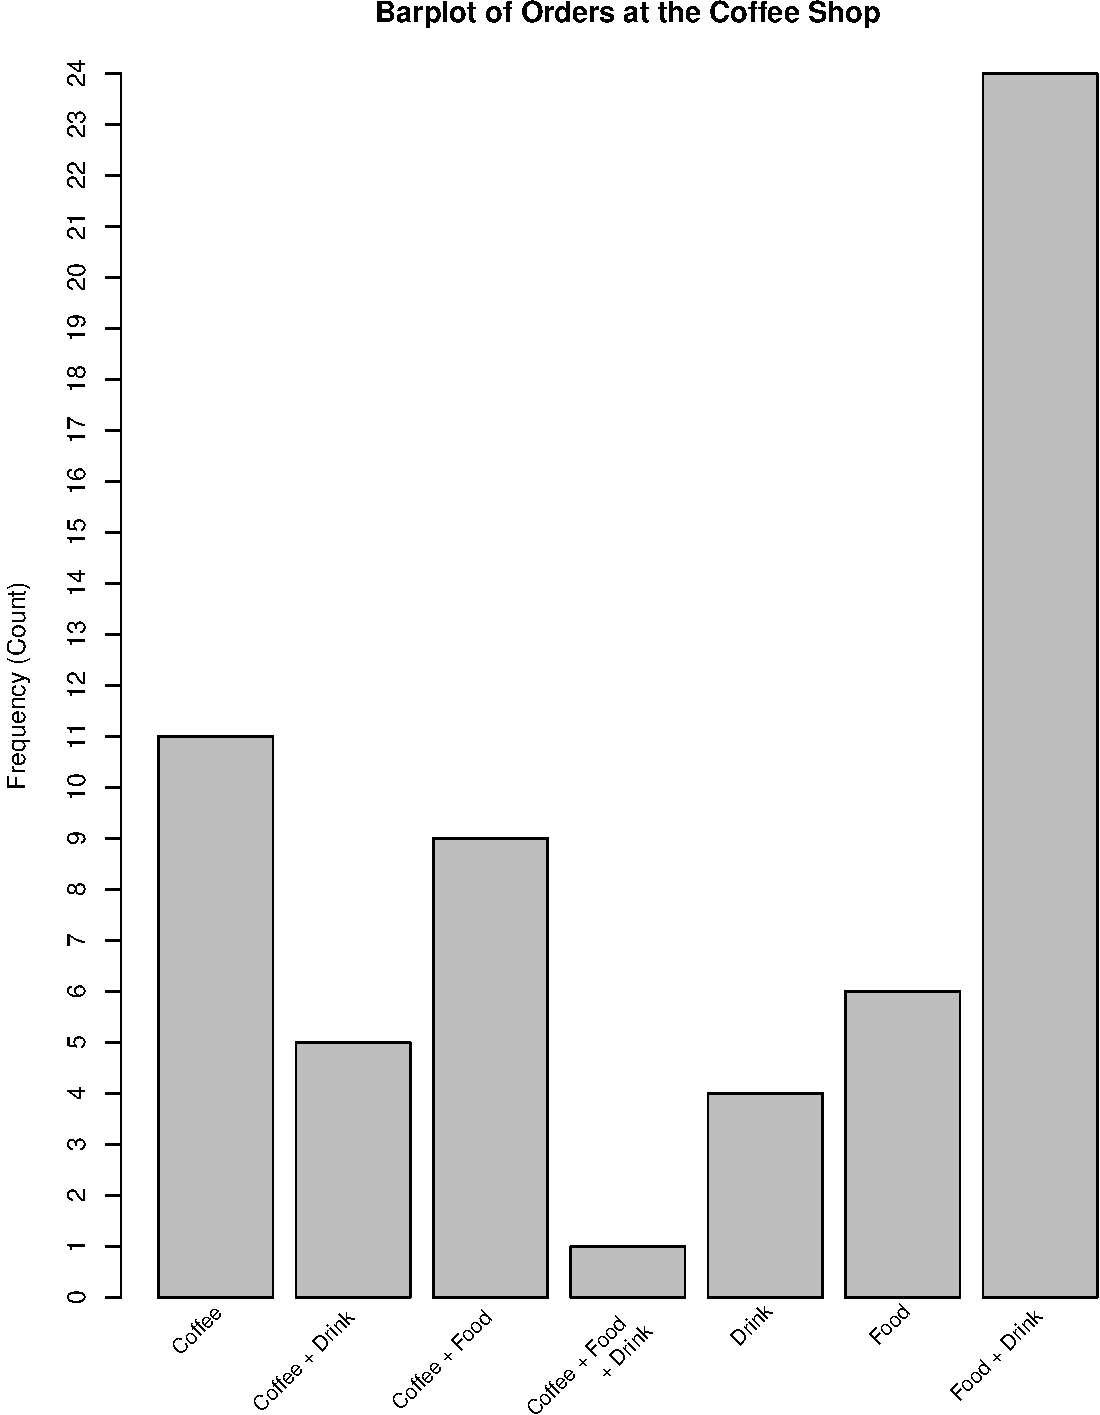
\includegraphics[keepaspectratio]{notes/chapter11_files/figure-pdf/sadie_coffee_barplot-1.pdf}}

Based on this plot, answer the following questions.

\begin{enumerate}
\def\labelenumi{\alph{enumi}.}
\tightlist
\item
  Which is the most common order in the sample, and what is the
  frequency with which it is ordered?
\item
  If there are a total of \(60\) orders, what is the relative frequency
  of the least common order?
\item
  How many orders had any coffee drink in the order?
\item
  Describe the overall frequency distribution.
\end{enumerate}

\begin{tcolorbox}[enhanced jigsaw, arc=.35mm, rightrule=.15mm, breakable, bottomrule=.15mm, left=2mm, toprule=.15mm, leftrule=.75mm, opacityback=0, colback=white, colframe=quarto-callout-color-frame]

\vspace{-3mm}\textbf{Solution}\vspace{3mm}

\begin{enumerate}
\def\labelenumi{\alph{enumi}.}
\tightlist
\item
  In this sample, there are \(24\) orders of Food + Drink, which is the
  most common order.
\item
  The least common order is a coffee + food + drink, which occurred
  \(\dfrac{1}{60} = 0.01666\) proportion of the time in the sample.
\item
  In total there were \(11 + 5 + 9 + 1 = 26\) orders with coffee in
  them. This accounts for \(\dfrac{26}{60} = 0.433333\) of all orders.
\item
  The most common order was food and a non-coffee drink, which was more
  than twice as common as the next most frequent order of just a coffee.
  It was very unlikely for people to get all three categories of item.
  People got coffee with food more frequently than food alone, drinks
  alone, or coffee with drinks.
\end{enumerate}

\end{tcolorbox}

\end{example}

Whenever we present a descriptive statistic, be that a numerical summary
or a graphical summary, it is always worth asking the question: ``what
are we trying to highlight?'' In the case of frequency distributions, we
are typically thinking about highlighting the total counts and cross
category comparisons of the different values. Often times these are
comparisons that we wish to make and using a bar chart for this is quite
effective. However, depending on what we are trying to communicate,
there may be alternative choices that make sense to make. It is always
important to ensure that your visualization or summary is informed by
the goal of your presentation, rather than by outside guidance.
Descriptive statistics is fundamentally a field predicated upon
communication. With that said, any time that we are presented with an
observed qualitative variable, the frequency distribution completely
contains all of the information in the data. It may not always be the
most useful presentation of the data, however, it is a way of
summarizing everything that we know about that variable alone. As a
result, deep comfort with frequency distributions will be instrumental
to effective communication and description of qualitative data.

\begin{example}[Charles finds Palmer's
Penguins]\protect\hypertarget{exm-palmer-penguins}{}\label{exm-palmer-penguins}

While daydreaming one day, Charles imagines the chance to work at the
Palmer Station in Antarctica, researching penguins. The day dreams lead
to a rich imagination, envisioning all species of penguins across the
various islands. As the day dreams wind-on, Charles begins to count the
penguins, leading to the following observations.

\begin{longtable*}[t]{>{}lrrr}
\toprule
 & Biscoe & Dream & Torgersen\\
\midrule
\textbf{Adelie} & 44 & 56 & 52\\
\textbf{Chinstrap} & 0 & 68 & 0\\
\textbf{Gentoo} & 124 & 0 & 0\\
\bottomrule
\end{longtable*}

Using these data\footnote{Horst AM, Hill AP, Gorman KB (2020).
  palmerpenguins: Palmer Archipelago (Antarctica) penguin data. R
  package Version 0.1.0. https://allisonhorst.github.io/palmerpenguins/.
  doi:10.5281/zenodo.3960218.} answer the following.

\begin{enumerate}
\def\labelenumi{\alph{enumi}.}
\tightlist
\item
  Write down the complete frequency distribution for penguin species.
\item
  Write down the complete frequency distribution for the inhabited
  island.
\item
  Describe or sketch the bar plots for each of the relevant frequency
  distributions.
\end{enumerate}

\begin{tcolorbox}[enhanced jigsaw, arc=.35mm, rightrule=.15mm, breakable, bottomrule=.15mm, left=2mm, toprule=.15mm, leftrule=.75mm, opacityback=0, colback=white, colframe=quarto-callout-color-frame]

\vspace{-3mm}\textbf{Solution}\vspace{3mm}

\begin{enumerate}
\def\labelenumi{\alph{enumi}.}
\tightlist
\item
  To get the distribution for species, we add up along each row to get
  the total observed data into a frequency table. The relative frequency
  is divided by \(344\).
\end{enumerate}

\begin{longtable*}[t]{>{}lrr}
\toprule
 & Frequency & Relative Frequency\\
\midrule
\textbf{Adelie} & 152 & 0.4418605\\
\textbf{Chinstrap} & 68 & 0.1976744\\
\textbf{Gentoo} & 124 & 0.3604651\\
\bottomrule
\end{longtable*}

\begin{enumerate}
\def\labelenumi{\alph{enumi}.}
\setcounter{enumi}{1}
\tightlist
\item
  To get the distribution for locations, we add up along each column to
  get the total observed data into a frequency table.
\end{enumerate}

\begin{longtable*}[t]{>{}lrr}
\toprule
 & Frequency & Relative Frequency\\
\midrule
\textbf{Biscoe} & 168 & 0.4883721\\
\textbf{Dream} & 124 & 0.3604651\\
\textbf{Torgersen} & 52 & 0.1511628\\
\bottomrule
\end{longtable*}

\begin{enumerate}
\def\labelenumi{\alph{enumi}.}
\setcounter{enumi}{2}
\tightlist
\item
  The following represent the two bar plots for each distribution.
\end{enumerate}

\begin{figure}[H]

\begin{minipage}{0.50\linewidth}
\pandocbounded{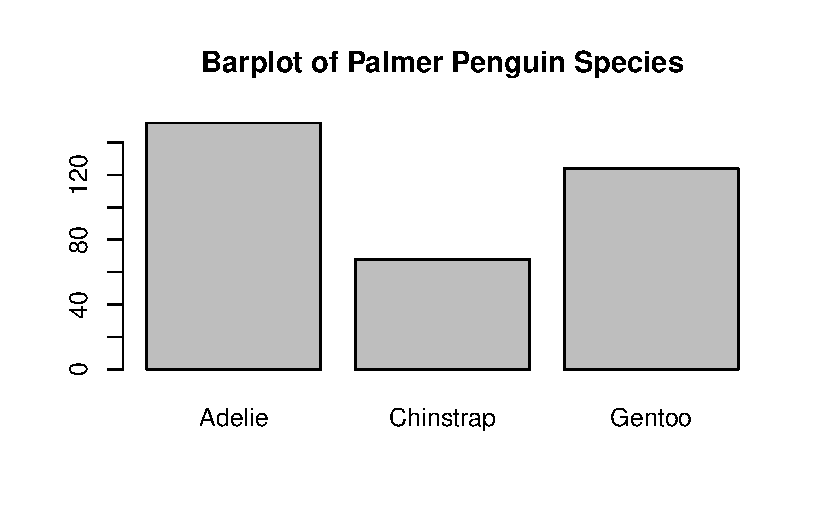
\includegraphics[keepaspectratio]{notes/chapter11_files/figure-pdf/penguin_bar_plot-1.pdf}}\end{minipage}%
%
\begin{minipage}{0.50\linewidth}
\pandocbounded{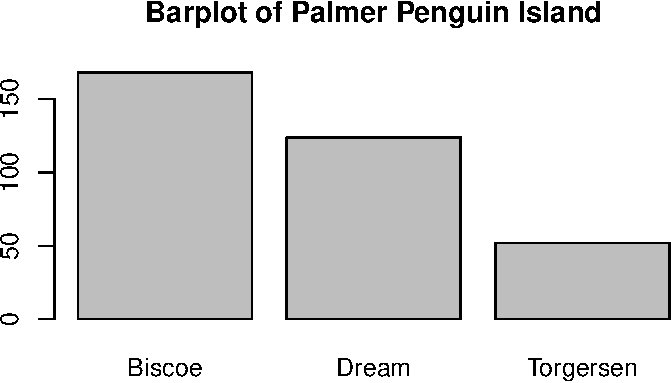
\includegraphics[keepaspectratio]{notes/chapter11_files/figure-pdf/penguin_bar_plot-2.pdf}}\end{minipage}%

\end{figure}%

\end{tcolorbox}

\end{example}

\section{Descriptive Statistics for Quantitative
Variables}\label{descriptive-statistics-for-quantitative-variables}

Where our approach for qualitative data was to first summarize the data
numerically, and then analyze, with quantitative data the first step is
unnecessary. When our data are numeric to begin, we can work directly
with them in order to begin to summarize the behaviour of the observed
variables. Despite this change in process, the frequency distribution
remains an impactful concept in summarizing and describing data which
have been observed.

\subsection{The Frequency Distribution for Quantitative
Variables}\label{the-frequency-distribution-for-quantitative-variables}

If the quantitative variables that have been observed are discrete, the
frequency distribution can proceed in an exactly equivalent way as in
the qualitative case. If, however, we have quantitative variables our
frequency distribution needs to be adjusted. The issue is that, if a
variable of interest is continuous, we do not expect to ever observe the
same value more than once. This renders the frequency distribution to
look something like a broken comb\footnote{\pandocbounded{\includegraphics[keepaspectratio]{graphics/ch11-broken_comb.png}}},
rather than having any interesting features. To avoid this happening, we
consider the process of \textbf{binning} quantitative variables, where
values are placed into \textbf{bins} or \textbf{classes}, consisting of
intervals, in order to better understand the structure of the frequency
distribution.

\begin{definition}[Data
Binning]\protect\hypertarget{def-data-binning}{}\label{def-data-binning}

Data binning is a (pre-processing) step of a data analysis in which
quantitative variables (typically continuous ones) are placed into
\textbf{bins} or \textbf{classes} based on their underlying value. If a
quantitative variable \(x\) takes values in the interval \([a,b]\), then
the interval \([a,b]\) is divided into several sub-intervals, say
\([a,p_1], [p_1, p_2], \dots, [p_{k-1},b]\). Then, each observed value
for \(x\), \(x_i\) is placed into its corresponding bin, before the data
are analyzed.

\end{definition}

As a general rule, bins should be selected either based on some
subject-matter justification (such that they are meaningful to the
underlying data), or else to accurately balance the trade-offs of
smoothness and accuracy in the frequency distribution. That is, we want
to select enough bins so that the true behaviour of the data are
correctly represented, while not selecting so many that noise and
variability are the primary conclusions to be drawn from the summaries.
Plenty of methods to select the number of bins have been proposed, and
in most software packages for devising frequency distributions various
techniques will be implemented. It is worth ensuring that the technique
selected for any particular use case accurately summarizes and describes
the available data. Generally, \(10-30\) bins will likely suffice,
though fewer or more may be necessary in certain situations.

The only hard-and-fast rules of binning is that, first, bins
should\footnote{Almost always.} be of equal width. That is, if you take
\([0,1)\) to be the first bin in your data, then every bin should be of
length \(1\). Second, bins should\footnote{Again, almost always.} span
the complete range of your observed data. If you have points ranging
from \(0\) to \(1000\), every value between \(0\) and \(1000\) should be
contained in some bin. Once binned, quantitative frequency distributions
can be described in exactly the same manner that qualitative were.

\begin{example}[Charles and Sadie Count Coffee Order
Items]\protect\hypertarget{exm-coffee-orders-counts}{}\label{exm-coffee-orders-counts}

After their success in understanding the makeup of different coffee
orders, Charles and Sadie set their sights on understanding the quantity
of items ordered by customers at the coffee shop. The observe customers
for an hour and consider the total number of items each customer orders.
The following observations are made.

\begin{itemize}
\tightlist
\item
  3
\item
  1
\item
  4
\end{itemize}

\begin{itemize}
\tightlist
\item
  2
\item
  1
\item
  1
\end{itemize}

\begin{itemize}
\tightlist
\item
  1
\item
  6
\item
  2
\end{itemize}

\begin{itemize}
\tightlist
\item
  3
\item
  1
\end{itemize}

\begin{itemize}
\tightlist
\item
  2
\item
  1
\end{itemize}

\begin{itemize}
\tightlist
\item
  3
\item
  2
\end{itemize}

Based on these data, answer the following questions.

\begin{enumerate}
\def\labelenumi{\alph{enumi}.}
\tightlist
\item
  Write down the frequency distribution for the number of items on each
  order. Include the relative frequency for each observation.
\item
  Is data binning required for this frequency distribution? Describe.
\end{enumerate}

\begin{tcolorbox}[enhanced jigsaw, arc=.35mm, rightrule=.15mm, breakable, bottomrule=.15mm, left=2mm, toprule=.15mm, leftrule=.75mm, opacityback=0, colback=white, colframe=quarto-callout-color-frame]

\vspace{-3mm}\textbf{Solution}\vspace{3mm}

\begin{enumerate}
\def\labelenumi{\alph{enumi}.}
\tightlist
\item
  Here the relevant categories are \(\{1,2,3,4,5,6\}\). We get
\end{enumerate}

\begin{longtable}[]{@{}lcc@{}}
\toprule\noalign{}
Order Size & Frequency (Count) & Relative Frequency \\
\midrule\noalign{}
\endhead
\bottomrule\noalign{}
\endlastfoot
1 & \(6\) & \(6/15 = 0.4\) \\
2 & \(4\) & \(4/15 = 0.266666\) \\
3 & \(3\) & \(3/15 = 0.333333\) \\
4 & \(1\) & \(1/15 = 0.066666\) \\
5 & \(0\) & \(0/15 = 0\) \\
6 & \(1\) & \(1/15 = 0.066666\) \\
\end{longtable}

\begin{enumerate}
\def\labelenumi{\alph{enumi}.}
\setcounter{enumi}{1}
\tightlist
\item
  No.~These data are discrete, and given that there are only \(6\) total
  categories there would be no particular utility to binning here. If
  the data were continuous, or were discrete with sufficiently many
  categories so as to be better treated as continuous than discrete,
  then binning would be pertinent.
\end{enumerate}

\end{tcolorbox}

\end{example}

\begin{example}[Charles and Sadie Count Coffee Order
Values]\protect\hypertarget{exm-coffee-orders-values}{}\label{exm-coffee-orders-values}

As a final way of understanding the distribution of different coffee
orders, Charles and Sadie decide to observe the total cost of orders for
various customers coming through the store. The following observations
are made over the course of an hour.

\begin{itemize}
\tightlist
\item
  \$2.25
\item
  \$2.20
\item
  \$5.13
\end{itemize}

\begin{itemize}
\tightlist
\item
  \$1.30
\item
  \$2.02
\item
  \$4.91
\end{itemize}

\begin{itemize}
\tightlist
\item
  \$1.64
\item
  \$3.49
\item
  \$0.98
\end{itemize}

\begin{itemize}
\tightlist
\item
  \$2.97
\item
  \$3.84
\end{itemize}

\begin{itemize}
\tightlist
\item
  \$5.30
\item
  \$2.53
\end{itemize}

\begin{itemize}
\tightlist
\item
  \$2.45
\item
  \$4.66
\end{itemize}

Based on these data, answer the following questions.

\begin{enumerate}
\def\labelenumi{\alph{enumi}.}
\tightlist
\item
  Describe the considerations that should be made for bin sizes. Would a
  bin size of \(\$0.10\) be reasonable? What about one that is
  \(\$3.00\)?
\item
  Suppose that a bin size of \(\$0.50\) is used, starting at \(0.50\).
  Write down the frequency distribution.
\end{enumerate}

\begin{tcolorbox}[enhanced jigsaw, arc=.35mm, rightrule=.15mm, breakable, bottomrule=.15mm, left=2mm, toprule=.15mm, leftrule=.75mm, opacityback=0, colback=white, colframe=quarto-callout-color-frame]

\vspace{-3mm}\textbf{Solution}\vspace{3mm}

\begin{enumerate}
\def\labelenumi{\alph{enumi}.}
\tightlist
\item
  The smallest observed value is \(0.98\) and the largest observed value
  is \(5.30\). That means that our bins should encapsulate both of these
  end points, and be evenly spaced throughout. Because there are only
  \(15\) data points, we likely want fewer bins rather than more, to
  ensure that our bins are not predominantly empty or with single items.
  If we use \(0.10\), we would require \(43\) bins at least to include
  all of the data. This would guarantee that most bins were empty, and
  is far too small of a divide to be useful. If we used \(\$3.00\), we
  would span the full range in \(2\) to \(3\) bins. This is likely not
  particularly informative either, this time giving too little of a
  breakdown of the various values.
\item
  The following is the relevant frequency distribution.
\end{enumerate}

\begin{longtable}[]{@{}lcc@{}}
\toprule\noalign{}
Bin & Frequency (Count) & Relative Frequency \\
\midrule\noalign{}
\endhead
\bottomrule\noalign{}
\endlastfoot
\([0.50,1.00)\) & \(1\) & \(1/15 = 0.066666666\) \\
\([1.00,1.50)\) & \(1\) & \(1/15 = 0.066666666\) \\
\([1.50,2.00)\) & \(1\) & \(1/15 = 0.066666666\) \\
\([2.00,2.50)\) & \(4\) & \(4/15 = 0.266666666\) \\
\([2.50,3.00)\) & \(2\) & \(2/15 = 0.133333333\) \\
\([3.00,3.50)\) & \(1\) & \(1/15 = 0.066666666\) \\
\([3.50,4.00)\) & \(1\) & \(1/15 = 0.066666666\) \\
\([4.00,4.50)\) & \(0\) & \(0/15 = 0\) \\
\([4.50,5.00)\) & \(2\) & \(2/15 = 0.0.1333333\) \\
\([5.00,5.50)\) & \(2\) & \(2/15 = 0.0.1333333\) \\
\end{longtable}

\end{tcolorbox}

\end{example}

While the tabular representation of the frequency distribution for
quantitative variables is a relevant summary, and one which serves a key
role, we will see that there are far more ways of summarizing the
behaviour of quantitative variables. Before that, however, it is worth
determining how to graphically represent a quantitative frequency
distribution, through the use of histograms.

\subsection{Using Histograms for Visualizing Quantitative Frequency
Distributions}\label{using-histograms-for-visualizing-quantitative-frequency-distributions}

If we expand the idea of a barplot to quantitative variables, we get the
\textbf{histogram}. A histogram is primarily useful for displaying the
distribution of a single quantitative variable. To do so, the horizontal
(x-axis) represents the value of the variable of interest, and the
corresponding vertical (y-axis) represents the frequency with which that
value occurs in the data. That is, higher points correspond to more
frequently occurring values, and lower points correspond to less
frequently occurring values.

If the data are binned, then the histogram displays counts within the
bins rather than at the values themselves. Just as with a barplot, the
graphic proceeds by drawing a rectangle, with a height equal to the
frequency, and a width equal to the length of the interval. The larger
the rectangle, the more points that were observed in that range.

Sometimes, instead of having the y-axis measure the frequency, we may
take it to measure the \textbf{density} of falling in that range. The
density is given by the probability that a value in that range is
observed, divided by the width of the range. For instance, if \(10\) of
\(50\) observations fell between \(2\) and \(4\), then the height of the
rectangle using the density representation would be
\(\dfrac{10/50}{4-2} = 0.1\). So long as every bin has an equal width,
the same relative heights will occur whether using the frequency or
density versions.

A key difference between histograms and barplots is that, since the data
in a histogram are numeric, we typically consider the x-axis to be
continuous. This means that the bins of the histograms expand along the
complete axis, and adjacent bins will touch one another. In a barplot
there is separation between these categories since there are no values
between the two of them.

\begin{example}[Charles and Sadie Plot the Coffee
Orders]\protect\hypertarget{exm-coffee-orders}{}\label{exm-coffee-orders}

Charles and Sadie realize that to make sure that they have a full
understanding of the total spend that customers have at the coffee shop
they should likely collect more data, and data which are spread out
randomly over times of the day and days of the week. As a result, they
conduct another random survey. Once collected, both Charles and Sadie
produce histograms for the totals, as seen here.

\begin{figure}

\begin{minipage}{\linewidth}
\pandocbounded{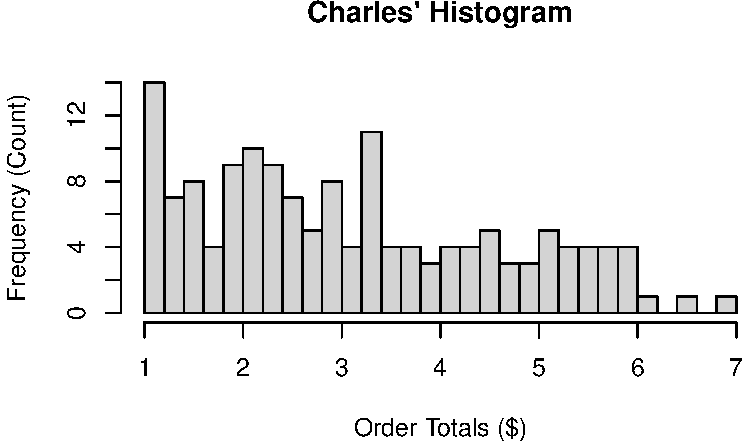
\includegraphics[keepaspectratio]{notes/chapter11_files/figure-pdf/coffee_sale_histograms-1.pdf}}\end{minipage}%
\newline
\begin{minipage}{\linewidth}
\pandocbounded{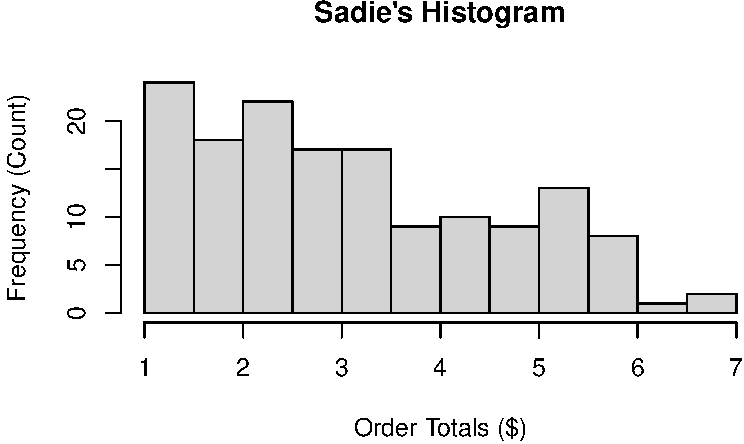
\includegraphics[keepaspectratio]{notes/chapter11_files/figure-pdf/coffee_sale_histograms-2.pdf}}\end{minipage}%

\end{figure}%

\begin{enumerate}
\def\labelenumi{\alph{enumi}.}
\tightlist
\item
  What is the approximate bin width used by Charles? By Sadie?
\item
  Describe the frequency distribution as depicted by both histograms.
\item
  Does one histogram do a better job than the other at representing
  these data? Explain.
\end{enumerate}

\begin{tcolorbox}[enhanced jigsaw, arc=.35mm, rightrule=.15mm, breakable, bottomrule=.15mm, left=2mm, toprule=.15mm, leftrule=.75mm, opacityback=0, colback=white, colframe=quarto-callout-color-frame]

\vspace{-3mm}\textbf{Solution}\vspace{3mm}

\begin{enumerate}
\def\labelenumi{\alph{enumi}.}
\tightlist
\item
  We can see that in every dollar along the x-axis, Sadie has two
  histogram rectangles. This suggests a bin width of approximately
  \(0.50\). For Charles, there are \(5\) per dollar, and as a result,
  the bin width will be approximately \(0.20\).
\item
  Both plots demonstrate that the most frequent order totals are
  comparatively low, with values around \(\$1.00\). With the histogram
  provided by Sadie, the order totals are fairly uniform between \(1\)
  and \(3.50\), with a small spike around \(2.00\). Following that, the
  order totals are fairly uniform between \(3.50\) and \(6\), before
  falling again above \(6.00\). The patterns in the histogram from
  Charles are similar, but with slightly more information. While there
  is a fairly uniform distribution of observations beyond \(3.40\), and
  then a dip beyond \(6.00\), for the smaller values there is an
  oscillating pattern. They spike around \(1.00\), \(2.00\), \(3.00\),
  and \(3.40\), with the other values being appreciably lower. Still,
  the lower values are definitely higher on average than the higher
  values, with roughly equivalent breakpoints as was seen with Sadie's.
\item
  The preferred histogram here will likely depend on the use case for
  the data. The data that Charles is demonstrating provides more
  specific information, however, it is possible that this added
  information is more noise than useful. It would be interesting to look
  at, for instance, the prices of various items at the store to see if
  there was a reason for the peaks: otherwise, it could be seen to be
  random variation that is not particularly noisy. Sadie's pattern, by
  contrast, is far more explicable, but it gains this by smoothing over
  a lot of the fine details within the graphic. Perhaps a graph that
  balances these two would be more suitable.
\end{enumerate}

\begin{figure}[H]

\begin{minipage}{\linewidth}
\pandocbounded{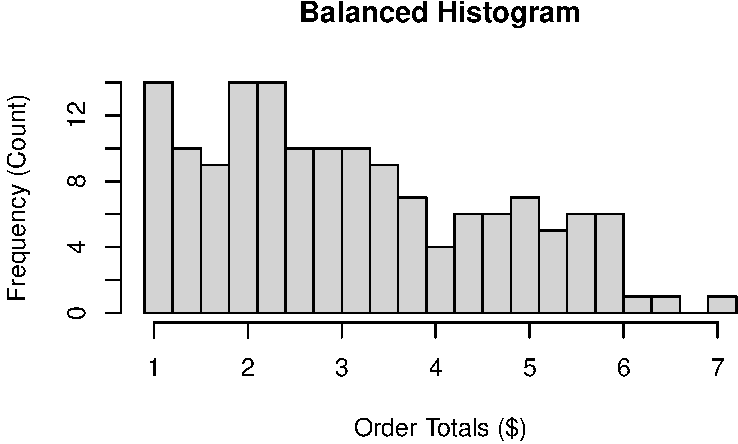
\includegraphics[keepaspectratio]{notes/chapter11_files/figure-pdf/coffee_sale_histogram_answer-1.pdf}}\end{minipage}%

\end{figure}%

\end{tcolorbox}

\end{example}

A histogram is a useful graphical display since it succinctly summarizes
the entire distribution of a particular variable. You can easily see the
range of the data, the points which came up frequently in your
observations, those which were rare, and how this behaviour is expressed
throughout. It will allow you to readily view points that appear to not
fit the trend of the rest of your data, and to investigate a single
variable at a glance.

When constructing a histogram, the primary decision that needs to be
made is how many bins you should use, or equivalently, how large your
bins should be. As you have more and more observations you can typically
get away with using smaller bin sizes as, even at the smaller sizes, you
likely still have observations that fall into the given intervals. Just
as with the discussion on data binning, software that implement
histogram construction often provide several techniques for choosing a
bin size, or the number of bins, in order to best summarize the data. It
is worth considering these for the problem at hand, and ensuring that
the choice that is made illustrates the data faithfully.

\subsection{Characteristics of the Frequency
Distribution}\label{characteristics-of-the-frequency-distribution}

While we will typically focus on graphically displaying the distribution
of a dataset, it is useful to consider what it is specifically that we
are trying to display, and what are the properties of a dataset which
are of interest to us? We are primarily concerned with three properties
of a distribution: the location, the spread, and the skewness. We have
seen all three of these concepts when discussing random variables, but
their importance becomes central when summarizing data. More concretely,
when describing data we want to make sure to describe the \textbf{shape}
of the distribution, the \textbf{centre} of the distribution, and the
\textbf{spread} of a distribution. Each of these three concepts have
different measures or components which, when taken together, serve as a
more complete description of the frequency distribution.

\begin{definition}[Shape (of a
Distribution)]\protect\hypertarget{def-shape}{}\label{def-shape}

The shape of the data distribution refers to the general pattern of
points that are observed in the specific dataset. Typically, the shape
of a distribution is decomposed into the \textbf{modality} and
\textbf{skewness} of the distribution.

The modality refers to the number of peaks that are visible in the
distribution: points that are higher than the surrounding points. A
distribution is unimodal with one peak, bimodal with two peaks, or
multimodal with more than two.

The skewness corresponds to how symmetric (or not) a distribution is. If
a distribution can be mirrored around its center, with the same
behaviour above and below the central point, we describe it as
symmetric. If a distribution has differing tail-behaviour, extending out
in a direction, we say that it is skewed. A distribution that has a
long-tail to the right is called \textbf{right skewed} or
\textbf{positive skewed}, where a distribution that has a long-tail to
the left is called \textbf{left skewed} or \textbf{negative skewed}.

\end{definition}

To describe the shape of a frequency distribution, we describe the
modality and the skewness of it. These two features combine to give a
good sense of the general picture of the distribution, such that someone
should be able to sketch a reasonable approximation to the frequency
distribution from the description. However, there are many distributions
with the same modality and skewness, which are otherwise quite distinct.
To understand these differences, it is useful to turn towards measures
of location, or central tendency, and measures of spread, or
variability.

\begin{definition}[Location (Central
Tendency)]\protect\hypertarget{def-location}{}\label{def-location}

The location of data, also referred to as the central tendency, is a
description of where observations in the dataset tended to fall around.
This can be measured as the sample mode, the sample median, or the
sample mean, and is typically summarized using all three. Measures of
central tendency give a sense as to where the middle of the data were,
where various definitions of middle can be used.

\end{definition}

Just as with random variables, measures of location come about by asking
what we ``expect'' to see in the data. When we are discussing samples,
rather than random variables, we are instead answering questions around
what we saw on average, or what we tended to see in the observed data.
Location summaries are quite common, and quite intuitive. You may
indicate the most common value, which is the sample mode, or the overall
average, the sample mean. However, just as with random variables, the
measures of central tendency only tell a partial story. The other key
feature of the data is the spread.

\begin{definition}[Spread
(Variability)]\protect\hypertarget{def-spread}{}\label{def-spread}

The spread of data is a measure of how separated the data are, and how
they tend to be spaced around the location. The spread can be captured
using particular measurements, such as the sample variance, sample IQR,
or sample range as was done with random variables. The may also refer to
the tail behaviour of the data, which looks at how likely values are as
they move further and further from the center of the data.

A distribution is said to be \textbf{heavy-tailed} if points that are
far from the measures of central tendency are quite frequent in the
data, and is said to be \textbf{light-tailed} otherwise. These concepts
can be formalized more rigorously, however, it is often taken to be an
informal rather than formal check.\footnote{Which is to say, we rely on
  the \emph{vibes} of the tails, rather than their mathematical
  behaviour explicitly.}

\end{definition}

The spread of the data gives a measure as to how concentrated (or not)
the observations were. Data which are widely spread out will have large
measures of variability compared to those which are less spread out.
When combined with the measures of central tendency, as well as a
description of the shape of the distribution, it is possible to develop
a fairly clear picture of the behaviour of the data, summarized rather
succinctly.

\subsection{The Shape of a
Distribution}\label{the-shape-of-a-distribution}

As indicated, the shape of a distribution is primarily defined by the
modality and skewness of the distribution. That is to say, when asked to
describe the shape of the distribution, you should report on the
modality (including the values of the modal points), as well as on the
symmetry or skewness of the distribution.

\begin{definition}[Modality]\protect\hypertarget{def-modality}{}\label{def-modality}

Modality refers to the number of \textbf{local} peaks that a frequency
distribution has. That is, the number of times that there are values in
the frequency distribution that are higher than those in close proximity
to them. If looking at the histogram we are looking for the number of
``hills'' that exist. Modality is classified by the number, and values,
of the different modal points.

A distribution with one local maximum is considered \textbf{unimodal}. A
distribution with two local maxima is considered \textbf{bimodal}. A
distribution with three or more local maxima is considered
\textbf{multimodal}.

\end{definition}

It is important to emphasize that a frequency distribution may have only
one mode, but may be multimodal. That is, we do not require each of the
peaks to tend to equate to exactly the same level to be considered
peaks. Instead, we compare them to only the points that are around them.
This way, we can capture the idea of \emph{local behaviour} indicating
that certain regions appeared more frequently than others around them,
which is often of direct interest to us. It is also important to
recognize that, if reading modal points from a histogram, the number of
breaks and the number of observations will likely change the perception
of the modality. There will often be judgment calls when discussing the
number of modes that a histogram exhibits, with reasonable disagreement
being possible. As a general rule, you should not consider small noisy
peaks adjacent to others to be additional modal points, unless there is
a good reason to do so. If you envision drawing a smooth line over the
full distribution of data, the modal points will come where you draw the
crests of the hills.

\begin{tcolorbox}[enhanced jigsaw, arc=.35mm, title={Identifying the Modality of Distributions}, rightrule=.15mm, coltitle=black, opacitybacktitle=0.6, colbacktitle=quarto-callout-tip-color!10!white, leftrule=.75mm, colback=white, breakable, titlerule=0mm, toptitle=1mm, bottomtitle=1mm, bottomrule=.15mm, toprule=.15mm, opacityback=0, left=2mm, colframe=quarto-callout-tip-color-frame]

\subsection*{Unimodal}\label{unimodal}
\addcontentsline{toc}{subsection}{Unimodal}

Data which exhibit a single peak, whether this is in the center or off
to one side, are considered to be \textbf{unimodal}.

\begin{figure}[H]

\begin{minipage}{0.33\linewidth}
\pandocbounded{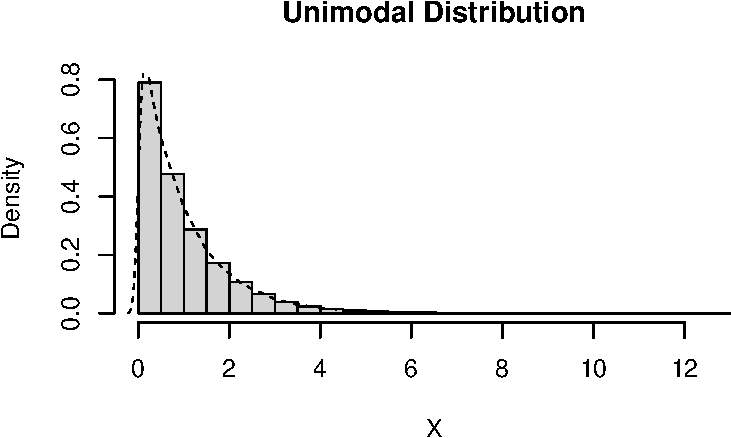
\includegraphics[keepaspectratio]{notes/chapter11_files/figure-pdf/unimodal_demo-1.pdf}}\end{minipage}%
%
\begin{minipage}{0.33\linewidth}
\pandocbounded{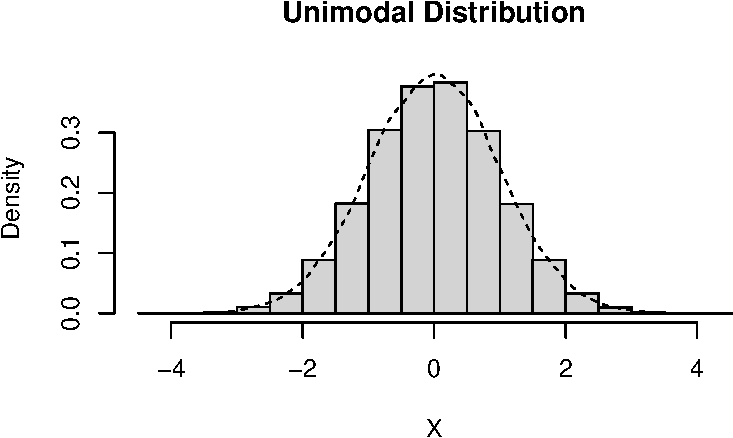
\includegraphics[keepaspectratio]{notes/chapter11_files/figure-pdf/unimodal_demo-2.pdf}}\end{minipage}%
%
\begin{minipage}{0.33\linewidth}
\pandocbounded{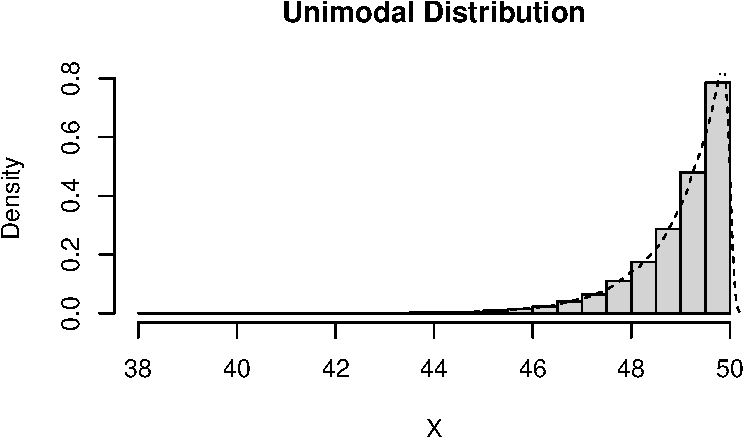
\includegraphics[keepaspectratio]{notes/chapter11_files/figure-pdf/unimodal_demo-3.pdf}}\end{minipage}%

\end{figure}%

\subsection*{Bimodal}\label{bimodal}
\addcontentsline{toc}{subsection}{Bimodal}

Data which exhibit exactly two peaks are considered to be
\textbf{bimodal}.

\begin{figure}[H]

\begin{minipage}{0.33\linewidth}
\pandocbounded{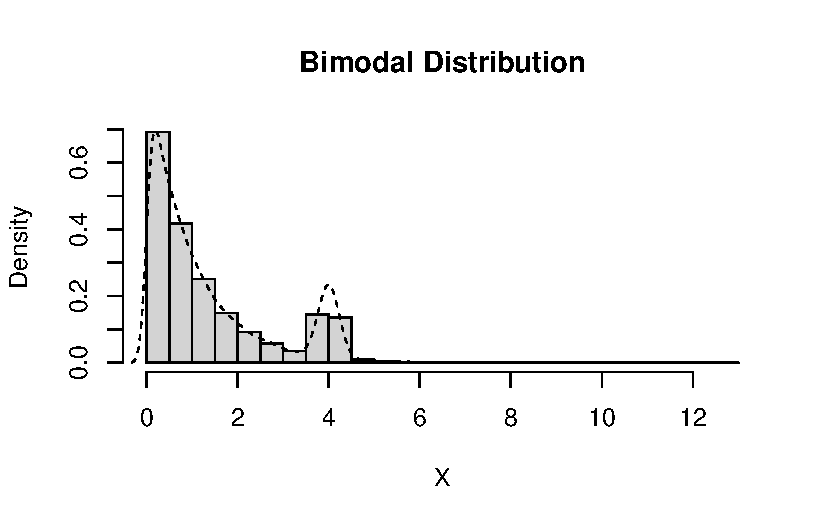
\includegraphics[keepaspectratio]{notes/chapter11_files/figure-pdf/bimodal_demo-1.pdf}}\end{minipage}%
%
\begin{minipage}{0.33\linewidth}
\pandocbounded{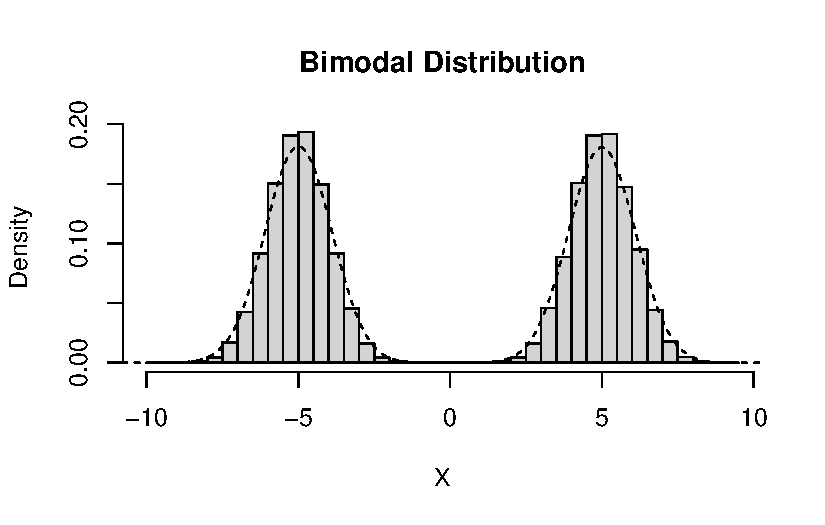
\includegraphics[keepaspectratio]{notes/chapter11_files/figure-pdf/bimodal_demo-2.pdf}}\end{minipage}%
%
\begin{minipage}{0.33\linewidth}
\pandocbounded{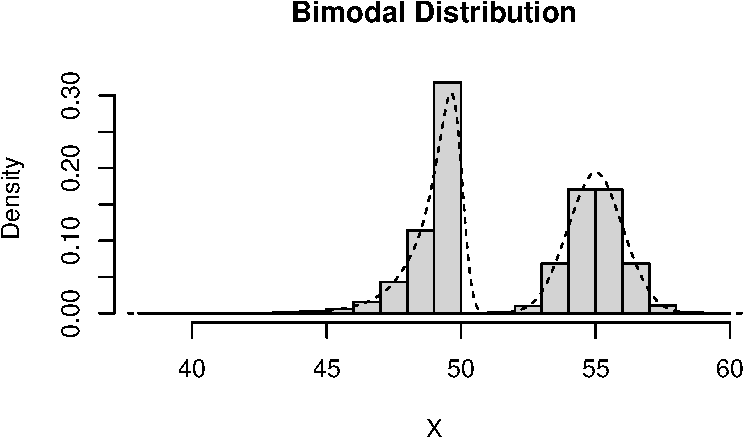
\includegraphics[keepaspectratio]{notes/chapter11_files/figure-pdf/bimodal_demo-3.pdf}}\end{minipage}%

\end{figure}%

\subsection*{Multimodal}\label{multimodal}
\addcontentsline{toc}{subsection}{Multimodal}

Data which exhibit more than two peaks are considered to be
\textbf{multimodal}.

\begin{figure}[H]

\begin{minipage}{0.33\linewidth}
\pandocbounded{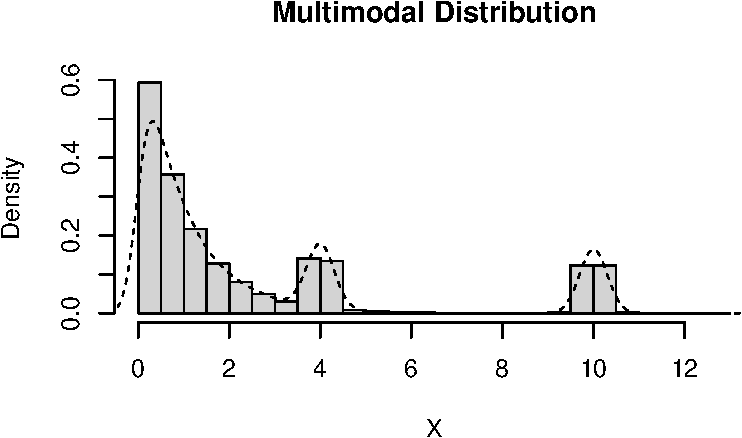
\includegraphics[keepaspectratio]{notes/chapter11_files/figure-pdf/mutlimodal_demo-1.pdf}}\end{minipage}%
%
\begin{minipage}{0.33\linewidth}
\pandocbounded{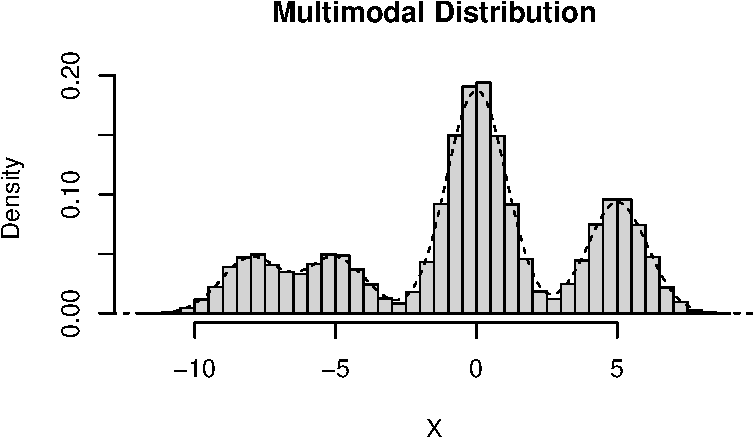
\includegraphics[keepaspectratio]{notes/chapter11_files/figure-pdf/mutlimodal_demo-2.pdf}}\end{minipage}%
%
\begin{minipage}{0.33\linewidth}
\pandocbounded{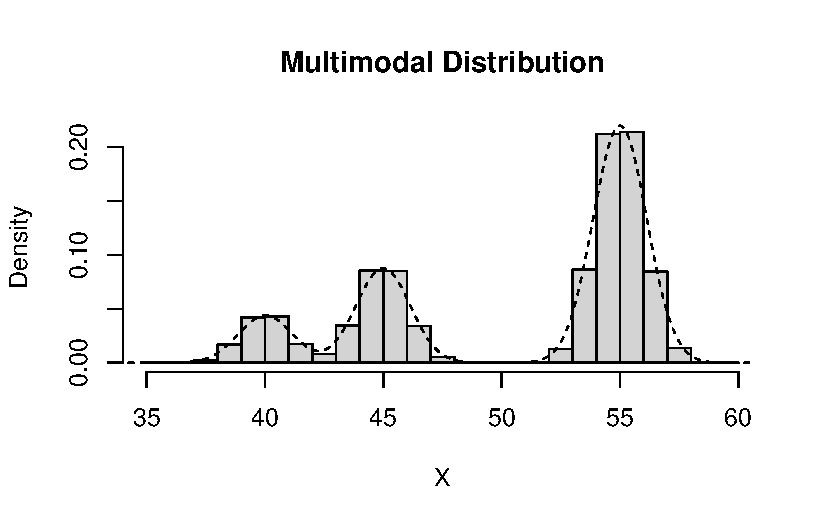
\includegraphics[keepaspectratio]{notes/chapter11_files/figure-pdf/mutlimodal_demo-3.pdf}}\end{minipage}%

\end{figure}%

\end{tcolorbox}

Beyond modality is the skewness. Skewness, or conversely, symmetry is a
way of describing the \textbf{tail behaviour} of a distribution. As you
move away from the central values, the most common values, or the middle
values of a distribution, the tails are the values that are far from
where you started but still present in the data. In general, if the
tails going to the positive and negative directions look similar, the
data are said to be symmetric. Otherwise, the data are said to be
skewed. We differentiate skewness based on the direction that the tail
travels.

\begin{definition}[Skewness]\protect\hypertarget{def-skewness}{}\label{def-skewness}

Data which are nonsymmetric are said to be skewed. The lack of symmetry
can be identified by the behaviour of the tails of a distribution,
differentiating between \textbf{positive} (or right) skew and
\textbf{negative} (or left) skew.

Data are right-skewed if the tail is longer to the righthand side of the
figure. Data are left-skewed if the tail is longer to the lefthand side
of the figure.

\end{definition}

Sometimes skewness is quite dramatic, being very evident in which
direction the skew will be. In other cases the data are not symmetric,
but are also not evidently skewed. In these settings it is worth
investigating the data in slightly more depth to try to understand
whether the lack of symmetry (or skewness) can be explained based on
some particular values, and if the remaining data exhibit a more
predictable pattern.

\begin{tcolorbox}[enhanced jigsaw, arc=.35mm, title={Identifying the Skewness of a Distribution}, rightrule=.15mm, coltitle=black, opacitybacktitle=0.6, colbacktitle=quarto-callout-tip-color!10!white, leftrule=.75mm, colback=white, breakable, titlerule=0mm, toptitle=1mm, bottomtitle=1mm, bottomrule=.15mm, toprule=.15mm, opacityback=0, left=2mm, colframe=quarto-callout-tip-color-frame]

To identify whether data are symmetric, right-skewed, or left-skewed,
you consider the beahviour of the tails.

\begin{figure}[H]

\begin{minipage}{0.33\linewidth}
\pandocbounded{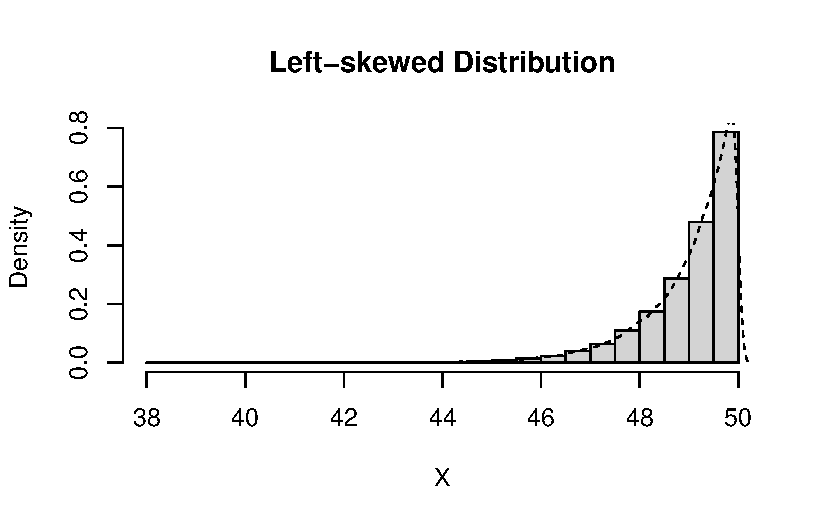
\includegraphics[keepaspectratio]{notes/chapter11_files/figure-pdf/skewness_of_distribution-1.pdf}}\end{minipage}%
%
\begin{minipage}{0.33\linewidth}
\pandocbounded{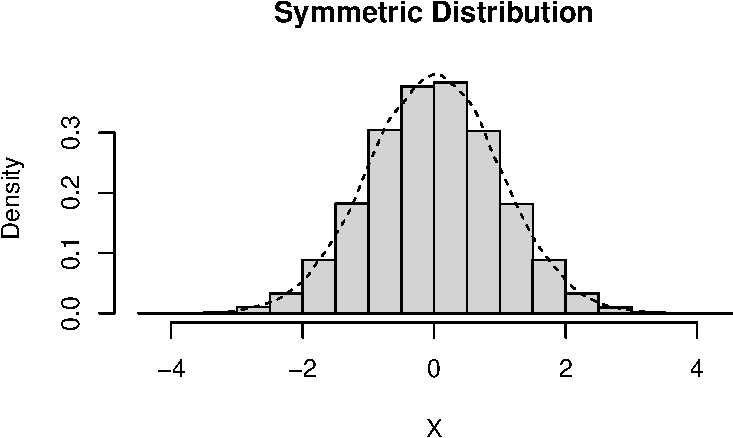
\includegraphics[keepaspectratio]{notes/chapter11_files/figure-pdf/skewness_of_distribution-2.pdf}}\end{minipage}%
%
\begin{minipage}{0.33\linewidth}
\pandocbounded{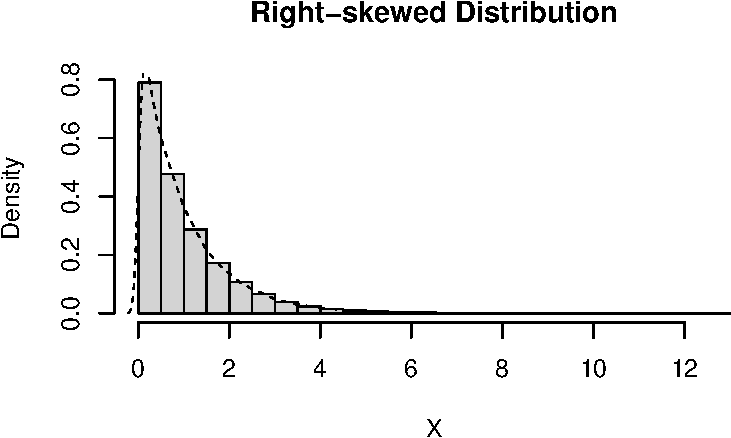
\includegraphics[keepaspectratio]{notes/chapter11_files/figure-pdf/skewness_of_distribution-3.pdf}}\end{minipage}%

\end{figure}%

\end{tcolorbox}

As a result, when asked to identify the shape of a distribution, you are
being asked about the key features of the distribution: how many modal
points are there, and where are those located, and what is happening
with the tails of the distribution? Beyond these points, discussion of
the shape of the distribution largely centers around giving added
context to the nuance with the provided descriptors. For instance, if
the skewness is not partiuclarly pronounced, that can be discussed. If
modal points are not clearly delineated, that should be acknowledged.
Once described, an individual should be able to sketch out a rough
distributional curve that approximately mirrors the behaviour of the
frequency distribution.

\begin{example}[Sadie Records the Timing of Hockey
Events]\protect\hypertarget{exm-charles-sadie-modality}{}\label{exm-charles-sadie-modality}

Sadie, being a big sports fan, has started to record and analyze the
timing of different events throughout the game. Charles decides to help
out by producing histograms for the time that these events happen at.
Sadie records the time that
\href{https://en.wikipedia.org/wiki/Face-off}{faceoffs} occur at, that
\href{https://en.wikipedia.org/wiki/Goal_(ice_hockey)}{goals} are scored
at, and when
\href{https://en.wikipedia.org/wiki/Penalty_(ice_hockey)}{penalties} are
taken.\footnote{For reference, NHL games are 60 minutes long
  (potentially longer if no one is winning at the end of the time),
  divided into 3 periods. When play is stopped, a face-off takes place
  to start the play again. Penalties occur when rules are violated by
  one of the teams. On the histograms, the start of the three periods
  are indicated in red dotted lines. These data come from a random
  sample of \(200\) games during the 2022-2023 NHL regular season.} The
histograms are provided below.

\pandocbounded{\includegraphics[keepaspectratio]{graphics/ch11-goal-hist.png}}

\pandocbounded{\includegraphics[keepaspectratio]{graphics/ch11-faceoff-hist.png}}

\pandocbounded{\includegraphics[keepaspectratio]{graphics/ch11-penalty-hist.png}}

\begin{enumerate}
\def\labelenumi{\alph{enumi}.}
\tightlist
\item
  Describe the shape of the distribution of goal times in NHL regular
  season games.
\item
  Describe the shape of the distribution of faceoff times in NHL regular
  season games.
\item
  Describe the shape of the distribution of penalty times in NHL regular
  season games.
\item
  Indicate any difficulties in describing these distributions.
\end{enumerate}

\begin{tcolorbox}[enhanced jigsaw, arc=.35mm, rightrule=.15mm, breakable, bottomrule=.15mm, left=2mm, toprule=.15mm, leftrule=.75mm, opacityback=0, colback=white, colframe=quarto-callout-color-frame]

\vspace{-3mm}\textbf{Solution}\vspace{3mm}

\begin{enumerate}
\def\labelenumi{\alph{enumi}.}
\tightlist
\item
  The distribution is approximately \textbf{bimodal}, with modal points
  at approximately \(30\) and \(60\) minutes. The distribution is
  non-symmetric, since higher frequency of goals are scored near the end
  of the game than at the beginning, making it a left-skewed
  distribution. If the final bin is ignored, which may be reasonable
  given that the final minute of game has different dynamics than other
  times, the distribution appears roughly symmetric.
\item
  This distribution is approximately \textbf{multimodal}. The modes
  occur at \(0\), \(20\), and \(40\) minutes. Every period starts with a
  faceoff, and as a result, every game will have faceoffs taken at
  exactly \(0\), \(20\), and \(40\) minutes into it. There are some
  points which may be described as modal points around \(10\) minutes
  and around \(30\) minutes, but these are far less obvious than the
  other three. The distribution is non-symmetric owing to the lack of a
  modal point at \(60\) minutes. Because of this, we may say that there
  is a slight positive skew to the distribution. It seems more sensible,
  however, to indicate that in the absence of the three modal points
  that are clearly explicable, it is a roughly symmetric distribution
  that is approximately uniform across the whole range.
\item
  The modality of the penalty timings is difficult to describe. It may
  be reasonable to describe this as multimodal with modes appear around
  \(20\), \(25\), \(38\), \(45\), and \(60\). However, this may also
  represent some histogram noise that is better to smooth over. In that
  case, perhaps you suggest that the three modal points are around
  \(20\), and \(40\), and around \(50\). The distribution does not
  exhibit perfect symmetry, owing to the spike near the end of the
  games, however, there seems to be little apparent skewness in the
  distribution. With the points near the end of the game removed, it is
  a mostly symmetric plot, however, with those points in there is some
  negative skewness indicated.
\item
  While the first two distributions are fairly clear to describe in
  shape, the penalties are a lot less evident. This becomes even more
  apparent when we consider how the number of bins selected impacts the
  overall shape of the distribution. Consider the following histograms
  (if online, you can click to enlarge them). With few bins, this
  distribution appears to be approximately symmetric with a single mode
  in the middle of the distribution. As more and more are added, the
  pattern remains rather similar until a within-period distribution
  emerges: the first period has a negative skew, unimodal distribution,
  the second a fairly uniform symmetric distribution, and the third a
  bimodal negative skew distribution. As we continue to add bins we see
  histograms that look similar to the one we considered, before getting
  to a point that looks more or less consistent throughout the range,
  with seemingly random spikes at various times. These demonstrate the
  importance of bin size selection, and illustrate the challenges that
  can occur when trying to describe real-world data.
\end{enumerate}

\begin{figure}[H]

\begin{minipage}{0.20\linewidth}
\pandocbounded{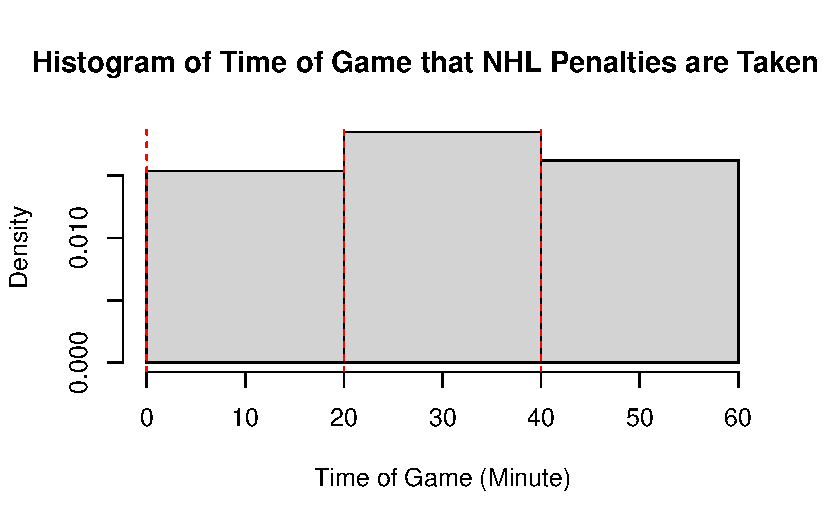
\includegraphics[keepaspectratio]{notes/chapter11_files/figure-pdf/penalty_hist-1.pdf}}\end{minipage}%
%
\begin{minipage}{0.20\linewidth}
\pandocbounded{\includegraphics[keepaspectratio]{notes/chapter11_files/figure-pdf/penalty_hist-2.pdf}}\end{minipage}%
%
\begin{minipage}{0.20\linewidth}
\pandocbounded{\includegraphics[keepaspectratio]{notes/chapter11_files/figure-pdf/penalty_hist-3.pdf}}\end{minipage}%
%
\begin{minipage}{0.20\linewidth}
\pandocbounded{\includegraphics[keepaspectratio]{notes/chapter11_files/figure-pdf/penalty_hist-4.pdf}}\end{minipage}%
%
\begin{minipage}{0.20\linewidth}
\pandocbounded{\includegraphics[keepaspectratio]{notes/chapter11_files/figure-pdf/penalty_hist-5.pdf}}\end{minipage}%
\newline
\begin{minipage}{0.20\linewidth}
\pandocbounded{\includegraphics[keepaspectratio]{notes/chapter11_files/figure-pdf/penalty_hist-6.pdf}}\end{minipage}%
%
\begin{minipage}{0.20\linewidth}
\pandocbounded{\includegraphics[keepaspectratio]{notes/chapter11_files/figure-pdf/penalty_hist-7.pdf}}\end{minipage}%
%
\begin{minipage}{0.20\linewidth}
\pandocbounded{\includegraphics[keepaspectratio]{notes/chapter11_files/figure-pdf/penalty_hist-8.pdf}}\end{minipage}%
%
\begin{minipage}{0.20\linewidth}
\pandocbounded{\includegraphics[keepaspectratio]{notes/chapter11_files/figure-pdf/penalty_hist-9.pdf}}\end{minipage}%
%
\begin{minipage}{0.20\linewidth}
\pandocbounded{\includegraphics[keepaspectratio]{notes/chapter11_files/figure-pdf/penalty_hist-10.pdf}}\end{minipage}%
\newline
\begin{minipage}{0.20\linewidth}
\pandocbounded{\includegraphics[keepaspectratio]{notes/chapter11_files/figure-pdf/penalty_hist-11.pdf}}\end{minipage}%
%
\begin{minipage}{0.20\linewidth}
\pandocbounded{\includegraphics[keepaspectratio]{notes/chapter11_files/figure-pdf/penalty_hist-12.pdf}}\end{minipage}%
%
\begin{minipage}{0.20\linewidth}
\pandocbounded{\includegraphics[keepaspectratio]{notes/chapter11_files/figure-pdf/penalty_hist-13.pdf}}\end{minipage}%
%
\begin{minipage}{0.20\linewidth}
\pandocbounded{\includegraphics[keepaspectratio]{notes/chapter11_files/figure-pdf/penalty_hist-14.pdf}}\end{minipage}%
%
\begin{minipage}{0.20\linewidth}
\pandocbounded{\includegraphics[keepaspectratio]{notes/chapter11_files/figure-pdf/penalty_hist-15.pdf}}\end{minipage}%
\newline
\begin{minipage}{0.20\linewidth}
\pandocbounded{\includegraphics[keepaspectratio]{notes/chapter11_files/figure-pdf/penalty_hist-16.pdf}}\end{minipage}%
%
\begin{minipage}{0.20\linewidth}
\pandocbounded{\includegraphics[keepaspectratio]{notes/chapter11_files/figure-pdf/penalty_hist-17.pdf}}\end{minipage}%
%
\begin{minipage}{0.20\linewidth}
\pandocbounded{\includegraphics[keepaspectratio]{notes/chapter11_files/figure-pdf/penalty_hist-18.pdf}}\end{minipage}%
%
\begin{minipage}{0.20\linewidth}
\pandocbounded{\includegraphics[keepaspectratio]{notes/chapter11_files/figure-pdf/penalty_hist-19.pdf}}\end{minipage}%

\end{figure}%

\end{tcolorbox}

\end{example}

\subsection{Measures of Location}\label{measures-of-location}

The shape of a distribution is described in fairly general terms. If you
know that a distribution is right-skewed and unimodal, with a peak
around \(10\), there are many plausible distributions that could be
drawn for what this would look like. While often times this shape
captures the most pertinent information for a distribution, sometimes we
require more. To add specificity, we can consider the location or
central tendency of a frequency distribution. The main measures of
location are the sample mean, sample median, and sample mode. These
correspond to the exact quantities that we saw in random variables, this
time computed on the data directly.

\begin{definition}[Sample
Mode]\protect\hypertarget{def-sample-mode}{}\label{def-sample-mode}

The sample mode is the most common value observed in a dataset. When
there are more than one value which appear equally often, these are all
consider modes. If a variable is binned, we may define the mode in terms
of the classes rather than the specific value, depending on the context.

\end{definition}

Whichever value appears most often is given as the mode. This is
analogous to the most probable value for a random variable. The sample
mode and the modal points are related to one another. When discussing
modality, we contented ourselves with approximations, considering values
\emph{near} the actual modal points when defining the peaks. When
discussing the sample mode we are looking for a specific value, or a
specific category of values, which actually gives the most frequent
value.

\begin{definition}[Sample
Median]\protect\hypertarget{def-sample-median}{}\label{def-sample-median}

The sample median is the middle point after ordering the observed data.
If there are an even number of observations it is the mean between the
two middle points. If we order the observed data as
\(x_{(1)} \leq x_{(2)} \leq \cdots \leq x_{(n)}\), then the median is
defined as \[\text{Median} = \begin{cases}
    x_{([n+1]/2)} & n \text{ is odd}; \\
    \dfrac{1}{2}\left(x_{(n/2)} + x_{(n/2 + 1)}\right) & n \text{ is even}.
\end{cases}\] That is, it is the middle point when there is an odd
number of observations in the data, and it is the average of the two
middle points when there are an even number of observations.

\end{definition}

The sample median has the same interpretation as the population median
we previously saw. There will always be \(50\%\) of the observations
which are less than or equal to the median, and always \$50\% of the
observations which are greater than or equal to the median. This puts
the median as the center of the distribution, when measured in terms of
frequencies.

\begin{definition}[Sample
Mean]\protect\hypertarget{def-sample-mean}{}\label{def-sample-mean}

The sample mean is the standard arithmetic average. If we observe
\(x_1,\dots,x_n\), then we write the mean as \(\overline{x}\), and this
is calculated as \[\overline{x} = \frac{1}{n}\sum_{i=1}^n x_i.\]

\end{definition}

The mean is a very commonly reported measure for the center of a
distribution. it is also referred to as the average. Just as with random
variables and the expected value, the mean can be viewed as balancing
the mass of observations. If you place equal mass at each of the
observations, then the mean would be the point which balances a seesaw
holding those masses.

\begin{example}[Charles' Penguin Bill
Lengths]\protect\hypertarget{exm-compute-central-tendency}{}\label{exm-compute-central-tendency}

Continuing on in day-dreaming adventures at the Palmer Station in
Antarctica, Charles envisions recording the bill lengths of a random
sampling of the penguins that are observed. These day-dreamed values are
recorded, and Charles would look to summarize the general behaviour of
these points, considering the measures of central tendency of them.

\begin{longtable}[]{@{}
  >{\centering\arraybackslash}p{(\linewidth - 18\tabcolsep) * \real{0.1000}}
  >{\centering\arraybackslash}p{(\linewidth - 18\tabcolsep) * \real{0.1000}}
  >{\centering\arraybackslash}p{(\linewidth - 18\tabcolsep) * \real{0.1000}}
  >{\centering\arraybackslash}p{(\linewidth - 18\tabcolsep) * \real{0.1000}}
  >{\centering\arraybackslash}p{(\linewidth - 18\tabcolsep) * \real{0.1000}}
  >{\centering\arraybackslash}p{(\linewidth - 18\tabcolsep) * \real{0.1000}}
  >{\centering\arraybackslash}p{(\linewidth - 18\tabcolsep) * \real{0.1000}}
  >{\centering\arraybackslash}p{(\linewidth - 18\tabcolsep) * \real{0.1000}}
  >{\centering\arraybackslash}p{(\linewidth - 18\tabcolsep) * \real{0.1000}}
  >{\centering\arraybackslash}p{(\linewidth - 18\tabcolsep) * \real{0.1000}}@{}}
\toprule\noalign{}
\endhead
\bottomrule\noalign{}
\endlastfoot
49.0 & 37.8 & 45.8 & 39.0 & 43.2 & 48.8 & 37.8 & 49.1 & 40.9 & 37.3 \\
\end{longtable}

\begin{enumerate}
\def\labelenumi{\alph{enumi}.}
\tightlist
\item
  What is the sample mean of these data?
\item
  What is the sample median of these data?
\item
  What is the sample mode of these data?
\item
  What is the expected value for the bill length in the population?
  Explain.
\end{enumerate}

\begin{tcolorbox}[enhanced jigsaw, arc=.35mm, rightrule=.15mm, breakable, bottomrule=.15mm, left=2mm, toprule=.15mm, leftrule=.75mm, opacityback=0, colback=white, colframe=quarto-callout-color-frame]

\vspace{-3mm}\textbf{Solution}\vspace{3mm}

\begin{enumerate}
\def\labelenumi{\alph{enumi}.}
\item
  For the sample mean, we compute \begin{align*}
  \overline{x} &= \frac{1}{10}(49.0 +  37.8 + 45.8 + 39.0 + 43.2 + 48.8 +  37.8 + 49.1 + 40.9 + 37.3) \\
  &= \frac{428.7}{10} \\
  &= 42.87
  \end{align*}
\item
  For the median, we first consider ordering the values in ascending
  order.
\end{enumerate}

\begin{longtable}[]{@{}
  >{\centering\arraybackslash}p{(\linewidth - 18\tabcolsep) * \real{0.1000}}
  >{\centering\arraybackslash}p{(\linewidth - 18\tabcolsep) * \real{0.1000}}
  >{\centering\arraybackslash}p{(\linewidth - 18\tabcolsep) * \real{0.1000}}
  >{\centering\arraybackslash}p{(\linewidth - 18\tabcolsep) * \real{0.1000}}
  >{\centering\arraybackslash}p{(\linewidth - 18\tabcolsep) * \real{0.1000}}
  >{\centering\arraybackslash}p{(\linewidth - 18\tabcolsep) * \real{0.1000}}
  >{\centering\arraybackslash}p{(\linewidth - 18\tabcolsep) * \real{0.1000}}
  >{\centering\arraybackslash}p{(\linewidth - 18\tabcolsep) * \real{0.1000}}
  >{\centering\arraybackslash}p{(\linewidth - 18\tabcolsep) * \real{0.1000}}
  >{\centering\arraybackslash}p{(\linewidth - 18\tabcolsep) * \real{0.1000}}@{}}
\toprule\noalign{}
\endhead
\bottomrule\noalign{}
\endlastfoot
37.3 & 37.8 & 37.8 & 39.0 & 40.9 & 43.2 & 45.8 & 48.8 & 49.0 & 49.1 \\
\end{longtable}

Then we note that the two middle values are \(40.9\) and \(43.2\), so we
get that \[\text{Median} = \frac{1}{2}(40.9 + 43.2) = 42.05.\]

\begin{enumerate}
\def\labelenumi{\alph{enumi}.}
\setcounter{enumi}{2}
\tightlist
\item
  The only repeated value in these data is \(37.8\), and so that makes
  it the mode.
\item
  We do not know, given this information, what the population expected
  value will be. We do not have access to enough information to compute
  the parameter, and instead must rely on using only our sample
  statistics. These are measures of the data that are observed, rather
  than the full population.
\end{enumerate}

\end{tcolorbox}

\end{example}

The three common measures of central tendency will often be explicitly
computed and reported when access to the data is directly available.
These can also be approximately indicated using a histogram of a
frequency distribution. The mode will be the bin with the highest
frequency, or equivalently, the highest point on the histogram. The
median will be found in the bin which contains the middle observation.
This can be challenging to find exactly without counting, but an
approximation is likely possible. The mean will be found in the bin
which balances the mass of the distribution. You can imagine asking
yourself: where would the fulcrum need to go in order to balance a
seesaw with these weights on it. The answer will tell you where the mean
is. Note that this process, without explicit observations, will not be
exact. Instead, it is in our interest to attempt to find approximately
correct solutions to these questions, getting a general sense of the
measures of central tendency from a graphical representation.

\begin{example}[Unknown Histogram
Markings]\protect\hypertarget{exm-identify-points}{}\label{exm-identify-points}

Charles wanted to help Sadie with the hockey analysis from before. To do
so, Charles worked out the mean, median, and mode for each of the
distributions, and indicated this on the histograms with black vertical
markings. Unfortunately, Charles does not remember which marking is
which. For each of the following graphics, indicate which of the three
solid vertical markings corresponds to the mean, median, and mode, or
describe why it is not possible to tell.

\begin{enumerate}
\def\labelenumi{\alph{enumi}.}
\tightlist
\item
  \pandocbounded{\includegraphics[keepaspectratio]{graphics/ch11-faceoff-plot-marked.png}}
\item
  \pandocbounded{\includegraphics[keepaspectratio]{graphics/ch11-heart-rate.png}}
\end{enumerate}

\begin{tcolorbox}[enhanced jigsaw, arc=.35mm, rightrule=.15mm, breakable, bottomrule=.15mm, left=2mm, toprule=.15mm, leftrule=.75mm, opacityback=0, colback=white, colframe=quarto-callout-color-frame]

\vspace{-3mm}\textbf{Solution}\vspace{3mm}

\begin{enumerate}
\def\labelenumi{\alph{enumi}.}
\tightlist
\item
  In this plot only two markings are differentiable from one another:
  one in the bin immediately before \(30\) and one in the bin
  immediately before \(40\). We know that the mode of the distribution
  falls into the bin around \(40\), and so the two lines here indicate
  the mean and the median. With the plot we should expect that the mean
  is slightly higher than the median, since the tail extends ever so
  slightly beyond symmetry to the positive side.
\item
  Here we can discern the mode to be marked around the \(80\) minute
  mark. The other two markings, for the mean and median, are marked in
  the bin just beyond \(40\). Here we know that the mean should be
  higher than the median, since the outlying spike later on will have
  the effect of pulling-up the observed mean, without impacting the
  median. Thus, we observe in order the median, mean, then mode.
\end{enumerate}

\end{tcolorbox}

\end{example}

It is also important to remember that, for each of these quantities,
when computed on a dataset, we refer to them as \emph{sample} measures.
That is, we call the mode the \textbf{sample mode}, the median the
\textbf{sample median}, and the mean the \textbf{sample mean}. This
terminology emphasizes that our calculations are not with respect to a
theoretical random variable with some assumed probability distribution,
but rather from a sample of data that was actually observed. Recall that
we view our sample as being \textbf{realizations} of a random quantity,
either as a random process or from a larger population. That is, we can
think of these measures as \textbf{statistics} computed on a sample,
rather than the \textbf{parameters} that could be computed on the
population.

\subsection{Measures of Spread or
Variability}\label{measures-of-spread-or-variability}

When we introduced the concept of the expected value, and other measures
of location of a random variable, we indicated that these would be
insufficient to accurately summarize the behaviour of a random quantity.
The same is true of a frequency distribution. Once again, by
complementing the measures of central tendency with measures of spread,
we are better able to understand the data which were actually observed,
and use this to inform our understanding of the data. Combining
variability, with central tendency, and distributional shape gives a
good overall picture of what was observed, in a digestible summary form.
The primary measures of variability for a dataset's distribution are the
same quantities used to measure variability of a random variable: the
(sample) variance, (sample) IQR, and (sample) range.

\begin{definition}[Sample
Range]\protect\hypertarget{def-sample-range}{}\label{def-sample-range}

The sample range is the observed range in the data set. We define the
sample range to be the difference between the maximum observed data
point and the minimum observed data point. That is, if the ordered data
is observed as \[x_{(1)} \leq x_{(2)} \leq \cdots \leq x_{(n)},\] then
the sample range is
\[\text{Range} = \max\{x\} - \min\{x\} = x_{(n)} - x_{(1)}.\] Just as
with the range of a random variable, the range may be reported as either
the distance between the minimum and maximum, or else as the minimum and
maximum points themselves.

\end{definition}

Just as with random variables, the sample range gives a rather coarse
view of variability within a datset. The sample range does give
information regarding the values that are \emph{possible}, based on what
was observed within the data, but it does not necessarily provide a
reasonable representation of which values were commonly expressed
throughout the data. A single outlying point can drramatically impact
the range, without meaningfully changing the observed patterns. For this
reason, we will often consider the sample IQR instead.

\begin{definition}[Sample Interquartile Range
(IQR)]\protect\hypertarget{def-sample-IQR}{}\label{def-sample-IQR}

The sample interquartile range is the difference between the first and
third quartiles in the dataset. That is, it is the length that spans the
middle \(50\%\) of observations within the variable. The sample IQR is
computed as \(\text{IQR} = Q3 - Q1\), where \(Q3\) and \(Q1\) are the
third and first quartiles.

In order to compute \(Q1\) you compute the median of the first half of
the data. In order to compute \(Q3\) you compute the median of the
second half of the data. If there are an odd number of points, the
central point is computed in both. That is, taking
\[x_{(1)} \leq x_{(2)} \leq \cdots \leq x_{(n)},\] then for the first
quartile,
\[Q1 = \begin{cases}\text{Median}\{x_{(1)}, x_{(2)},\dots, x_{(n/2)}\} & n \text{ even} \\ \text{Median}\{x_{(1)}, x_{(2)}, \dots, x_{([n+1]/2)}\} & n \text{ odd}\end{cases}.\]
The third quartile, \(Q3\), is computed similarly as
\[Q3 = \begin{cases}\text{Median}\{x_{(n/2+1)}, x_{(n/2 + 2)},\dots, x_{(n)}\} & n \text{ even} \\ \text{Median}\{x_{([n+1]/2)}, x_{([n+1]/2+1)}, \dots, x_{(n)}\} & n \text{ odd}\end{cases}.\]

\end{definition}

The interquartile range has the same benefits when compared to the range
in a sample as it did for random variables. Outlying points that
substantially deviate from the trends that are actually observed do not
make a large difference on the sample IQR, where they will on the sample
range. This can be desirable for understanding the variability in
\emph{most} of the data. Just as with random variables, the range and
IQR are analogous in that they give a full representation of how spread
out the data are. It is also possible to conceive of variability as how
far from \emph{average} data tend to be. For this, we consider the
sample variance (and standard deviation).

\begin{definition}[Sample
Variance]\protect\hypertarget{def-sample-variance}{}\label{def-sample-variance}

The sample variance is an analogue to the population variance, measuring
how far data are from the sample mean, on average. To compute the sample
variance we take the following form
\[s^2 = \frac{1}{n-1}\sum_{i=1}^n (x_i - \overline{x})^2.\] Note that
the division here is by \(n-1\) rather than by \(n\).\footnote{This
  makes the sample variance \textbf{unbiased} for the true variance. If
  you conceive of the sample variance as a random quantity, one that
  depends on what sample you actually take, dividing by \(n-1\) rather
  than by \(n\) will make it so that \(E[S^2] = \text{var}(X)\), where
  if you divide by \(n\) this will not be the case.} Notice that if
\(n\) is large, dividing by \(n\) or by \(n-1\) will give roughly the
same results.

\end{definition}

The sample variance has the same underlying concern as the variance of a
random variable: namely, it is a squared quantity. As a result, we will
often consider the \textbf{sample standard deviation}, which is given by
the square root of the sample variance, as an alternative representation
of the sample variability.

\begin{definition}[Sample Standard
Deviation]\protect\hypertarget{def-sample-sd}{}\label{def-sample-sd}

The sample standard deviation is an analogue to the population standard
deviation, giving an approximate measure of the mean deviation from the
sample mean, measured in the same units. The sample standard deviation
is given by the square root of the sample variance, which is to say
\[\text{SD} = s = \sqrt{s^2} = \sqrt{\frac{1}{n-1}\sum_{i=1}^n (x_i - \overline{x})^2}.\]

\end{definition}

These measures of spread are also useful to supplement the understanding
of the behaviour of a dataset that is provided by the measures of
central tendency. Specifically, by reporting measures of central
tendency, alongside measures of spread, and a description of the shape
of the distribution, you are able to describe and summarize the
beahviour of a dataset in a concise manner in such a way so as to allow
for a deep understanding of the patterns that have emerged.

\begin{example}[Sadie Questions the Spread in Bill
Lengths]\protect\hypertarget{exm-compute-spread}{}\label{exm-compute-spread}

After having described the central tendency of the bill length data that
Charles day dreamed about, Sadie inquires about the variability in the
data. Charles, so focused on the penguins themselves, had not even
stopped to consider how much variability may be present in these data.
Sadie decides to help out by computing measures of sample variability.

\begin{longtable}[]{@{}
  >{\centering\arraybackslash}p{(\linewidth - 18\tabcolsep) * \real{0.1000}}
  >{\centering\arraybackslash}p{(\linewidth - 18\tabcolsep) * \real{0.1000}}
  >{\centering\arraybackslash}p{(\linewidth - 18\tabcolsep) * \real{0.1000}}
  >{\centering\arraybackslash}p{(\linewidth - 18\tabcolsep) * \real{0.1000}}
  >{\centering\arraybackslash}p{(\linewidth - 18\tabcolsep) * \real{0.1000}}
  >{\centering\arraybackslash}p{(\linewidth - 18\tabcolsep) * \real{0.1000}}
  >{\centering\arraybackslash}p{(\linewidth - 18\tabcolsep) * \real{0.1000}}
  >{\centering\arraybackslash}p{(\linewidth - 18\tabcolsep) * \real{0.1000}}
  >{\centering\arraybackslash}p{(\linewidth - 18\tabcolsep) * \real{0.1000}}
  >{\centering\arraybackslash}p{(\linewidth - 18\tabcolsep) * \real{0.1000}}@{}}
\toprule\noalign{}
\endhead
\bottomrule\noalign{}
\endlastfoot
49.0 & 37.8 & 45.8 & 39.0 & 43.2 & 48.8 & 37.8 & 49.1 & 40.9 & 37.3 \\
\end{longtable}

\begin{enumerate}
\def\labelenumi{\alph{enumi}.}
\tightlist
\item
  What is the sample range of these data?
\item
  What is the sample IQR of these data?
\item
  What is the sample variance of these data? What is the sample standard
  deviation?
\item
  What is the variance of the bill lengths? Explain.
\end{enumerate}

\begin{tcolorbox}[enhanced jigsaw, arc=.35mm, rightrule=.15mm, breakable, bottomrule=.15mm, left=2mm, toprule=.15mm, leftrule=.75mm, opacityback=0, colback=white, colframe=quarto-callout-color-frame]

\vspace{-3mm}\textbf{Solution}\vspace{3mm}

The solution is made easier by first ordering the data. Consider

\begin{longtable}[]{@{}
  >{\centering\arraybackslash}p{(\linewidth - 18\tabcolsep) * \real{0.1000}}
  >{\centering\arraybackslash}p{(\linewidth - 18\tabcolsep) * \real{0.1000}}
  >{\centering\arraybackslash}p{(\linewidth - 18\tabcolsep) * \real{0.1000}}
  >{\centering\arraybackslash}p{(\linewidth - 18\tabcolsep) * \real{0.1000}}
  >{\centering\arraybackslash}p{(\linewidth - 18\tabcolsep) * \real{0.1000}}
  >{\centering\arraybackslash}p{(\linewidth - 18\tabcolsep) * \real{0.1000}}
  >{\centering\arraybackslash}p{(\linewidth - 18\tabcolsep) * \real{0.1000}}
  >{\centering\arraybackslash}p{(\linewidth - 18\tabcolsep) * \real{0.1000}}
  >{\centering\arraybackslash}p{(\linewidth - 18\tabcolsep) * \real{0.1000}}
  >{\centering\arraybackslash}p{(\linewidth - 18\tabcolsep) * \real{0.1000}}@{}}
\toprule\noalign{}
\endhead
\bottomrule\noalign{}
\endlastfoot
37.3 & 37.8 & 37.8 & 39.0 & 40.9 & 43.2 & 45.8 & 48.8 & 49.0 & 49.1 \\
\end{longtable}

\begin{enumerate}
\def\labelenumi{\alph{enumi}.}
\tightlist
\item
  The largest value is \(49.1\) and the smallest is \(37.3\). As a
  result the sample range is \(49.1 - 37.3 = 11.8\).
\item
  To find the sample IQR we find \(Q1\) and \(Q3\). There are \(10\)
  points, so \(Q1\) is the median of the first five, and \(Q3\) is the
  median of the last \(5\). The first five points are
  \(37.3, 37.8, 37.8, 39.0, 40.9\) so \(Q1 = 37.8\). The last \(5\)
  points are \(43.2, 45.8,  48.8, 49.0, 49.1\) so \(Q3 =  48.8\). Thus,
  the IQR is \(48.8 - 37.8 = 11\).
\item
  For the sample variance, we first note that (from
  Example~\ref{exm-compute-central-tendency}), we know that
  \(\overline{X} = 42.87\). Thus, we get \begin{align*}
  s^2 &= \frac{1}{n-1}\sum_{i=1}^n(x_i - \overline{x})^2 \\
  &= \frac{1}{9}\left((37.3 - 42.87)^2 + (37.8 - 42.87)^2 + (37.8-42.87)^2 + (39 - 42.87)^2\right. \\
  &\left.+ (40.9-42.87)^2 + (43.2-42.87)^2 + (45.8 - 42.87)^2 + (48.8 - 42.87)^2 + \right.\\
  &\left.(49 -42.87)^2 + (49.1 - 42.87)^2\right) \\
  &= 24.6156
  \end{align*} For the sample standard deviation, we simply take the
  square root fo this, giving \(s = \sqrt{24.6156} = 4.9615\).
\item
  We do not know, given this information, what the population variance
  will be. We do not have access to enough information to compute the
  parameter, and instead must rely on using only our sample statistics.
  These are measures of the data that are observed, rather than the full
  population.
\end{enumerate}

\end{tcolorbox}

\end{example}

\subsection{The Five Number Summary and
Boxplots}\label{the-five-number-summary-and-boxplots}

Histograms display a substantial amount of information for the entire
observed distribution. They display the shape of the distribution, as
well as the details as to which observations are likely or unlikely
values, allowing this to be seen in one place. This amount of detail is
often very useful, but on occasion it can obscure the larger picture.
This becomes particularly apparent when we wish to compare the
distribution of two different variables, or perhaps the same variable
across two or more categories. In these situations, the numeric
summaries that we have discussed end up holding more weight. While it is
very often to report the mean along with the standard deviation, as the
two values complement eachother well, it is also very common to report
the so-called \textbf{five number summary} of a data.

\begin{definition}[Five Number
Summary]\protect\hypertarget{def-five-number-summary}{}\label{def-five-number-summary}

The five number summary is a method for reporting a set of descriptive
statistics for a set of observed data. The five number summary consists
of five numbers, listed in order. This is given by
\[\min(x), Q1, \text{Median}(x), Q3, \max(x).\] That is, the five number
summary reports the minimum, the first quartile, the median, the third
quartile, and the maximum value from a dataset. Doing so provides a
succinct summary of both the location as well as the spread of observed
data.

\end{definition}

From the five number summary we also immediately know the range, and the
IQR. While it is useful to specifically report the values of the five
number summary, it can be even more effectively to display this
graphically. Boxplots are a graphical display which leverage this idea.
For a variable, the boxplot displays the minimum, the maximum, the
median, as well as the first and third quartiles \(Q1\) and \(Q3\), in
ascending order, for a given variable. In order to do this, a box is
drawn starting at \(Q1\) and going up to \(Q3\). Then, the median is
marked in the middle of this box. Extending from the box are the
\emph{whiskers}.

Each whisker is drawn out a length of \(1.5\) times the observed IQR,
stopping at the highest (or lowest) point within that range. Thus, if
all points fall within \(1.5\) times the IQR of either \(Q1\) or \(Q3\),
then the whiskers will stop at the minimum or maximum point observed. If
not, there are points beyond those included in the whiskers: these are
typically referred to as outliers. The outliers are drawn beyond the
whiskers of a boxplot, drawing a single dot for each point.

\begin{figure}[H]

\caption{\label{fig-boxplot-labels}A visual representation of a boxplot.
The five number summary is included, along with an indication of which
values fall outside of an expected range by using the whiskers to
indicate \(1.5\) times the IQR.}

\centering{

\pandocbounded{\includegraphics[keepaspectratio]{graphics/ch11-boxplot-labeled.png}}

}

\end{figure}%

\begin{example}[Boxplots and Numeric
Summaries]\protect\hypertarget{exm-boxplots-from-numeric-summaries}{}\label{exm-boxplots-from-numeric-summaries}

Charles and Sadie have gotten very much into the summarizing data from
the penguins. For the first sample of penguins, they have measurements
of bill lengths in mm, with the following observations.

\begin{longtable}[]{@{}
  >{\centering\arraybackslash}p{(\linewidth - 18\tabcolsep) * \real{0.1000}}
  >{\centering\arraybackslash}p{(\linewidth - 18\tabcolsep) * \real{0.1000}}
  >{\centering\arraybackslash}p{(\linewidth - 18\tabcolsep) * \real{0.1000}}
  >{\centering\arraybackslash}p{(\linewidth - 18\tabcolsep) * \real{0.1000}}
  >{\centering\arraybackslash}p{(\linewidth - 18\tabcolsep) * \real{0.1000}}
  >{\centering\arraybackslash}p{(\linewidth - 18\tabcolsep) * \real{0.1000}}
  >{\centering\arraybackslash}p{(\linewidth - 18\tabcolsep) * \real{0.1000}}
  >{\centering\arraybackslash}p{(\linewidth - 18\tabcolsep) * \real{0.1000}}
  >{\centering\arraybackslash}p{(\linewidth - 18\tabcolsep) * \real{0.1000}}
  >{\centering\arraybackslash}p{(\linewidth - 18\tabcolsep) * \real{0.1000}}@{}}
\toprule\noalign{}
\endhead
\bottomrule\noalign{}
\endlastfoot
49.0 & 37.8 & 45.8 & 39.0 & 43.2 & 48.8 & 37.8 & 49.1 & 40.9 & 37.3 \\
\end{longtable}

They took another two samples with other bill length measurements, but
seemed to have lost the data directly. Fortunately, they have the five
number summaries. These are given by the following.

\begin{longtable}[]{@{}cccccc@{}}
\toprule\noalign{}
Sample & Min & Q1 & Median & Q3 & Max \\
\midrule\noalign{}
\endhead
\bottomrule\noalign{}
\endlastfoot
2 & 32 & 40 & 43 & 45 & 52 \\
3 & 34 & 37 & 41 & 49 & 50 \\
\end{longtable}

\begin{enumerate}
\def\labelenumi{\alph{enumi}.}
\tightlist
\item
  Write down the five number summary for the first sample.
\item
  Sketch a boxplot for the first sample, or explain why it is not
  possible.
\item
  Sketch a boxplot for the second sample, or explain why it is not
  possible.
\item
  Sketch a boxplot for the third sample, or explain why it is not
  possible.
\end{enumerate}

\begin{tcolorbox}[enhanced jigsaw, arc=.35mm, rightrule=.15mm, breakable, bottomrule=.15mm, left=2mm, toprule=.15mm, leftrule=.75mm, opacityback=0, colback=white, colframe=quarto-callout-color-frame]

\vspace{-3mm}\textbf{Solution}\vspace{3mm}

\begin{enumerate}
\def\labelenumi{\alph{enumi}.}
\tightlist
\item
  In the previous examples, Example~\ref{exm-compute-central-tendency}
  and Example~\ref{exm-compute-spread}, we found that the five number
  summary would be given by \(37.3, 37.8, 42.05, 48.8, 49.1\).
\item
  The boxplot here will have a box drawn from \(37.8\) to \(48.8\), with
  a median line drawn at \(42.05\). The whiskers will extend for
  \(37.3\) which is only \(0.5\) beneath \(Q1\) and so there will be no
  outlier points drawn. The upper whisker will be drawn out to \(49.1\)
  which is only \(0.3\) above \(Q3\) and so it will be drawn without
  outlier points. This can be pictured as follows.
\end{enumerate}

\pandocbounded{\includegraphics[keepaspectratio]{notes/chapter11_files/figure-pdf/unnamed-chunk-13-1.pdf}}

\begin{enumerate}
\def\labelenumi{\alph{enumi}.}
\setcounter{enumi}{2}
\tightlist
\item
  In this case we will be unable to draw a boxplot for the sample. The
  issue is that the minimum point is \(32\) which is \(8\) below \(Q1\).
  The IQR is \(45 - 40 = 5\), and so \(1.5\times 5 = 7.5\). As a result,
  the minimum would need to be drawn as an outlier point, which means
  that we cannot know where the whiskers will stop. This concern is not
  present on the upper side, where the whisker would be extended to
  \(52\).
\item
  Here we can use the \(5\) number summary to draw the boxplot directly.
  The box would be drawn from \(37\) to \(49\), with the medina marked
  at \(41\). The whiskers would extend down to \(34\) (\(3\) below
  \(Q1\)) and up to \(50\) (\(1\) above \(Q3\)). This can be pictured as
  follows.
\end{enumerate}

\pandocbounded{\includegraphics[keepaspectratio]{notes/chapter11_files/figure-pdf/unnamed-chunk-14-1.pdf}}

\end{tcolorbox}

\end{example}

It is important to note that the boxplot is inspired by the five number
summary, but it encodes slightly more information. It will be precisely
the same whenever the maximum and minimum fall within \(1.5\) times the
IQR of the first and third quartiles, but it will include further
information in all other cases. This is done to indicate points which
are \textbf{outliers}, those which appear to deviate from expected
trends (of nicely behaved data).\footnote{Outliers are a topic that
  necessitate a great deal of discussion to approach with care. As a
  general rule, I would be skeptical of any analysis you see which
  excludes outliers on the basis of a statistical test. Outliers,
  especially as assessed from these types of rules, are better
  understood as points that demonstrate that the data are heavy-tailed
  rather than points which should be ignored.}

Typically, the boxplots will be drawn so that multiple plots are shown
on the same graph. In order to read a boxplot you can compare the
medians, and then the spread. The typical variability of the quantity is
contained within the box portion, and plots which have largely
overlapping boxes are often thought to behave similarly. The whiskers
represent the outer limits of what is expected within the data: if both
whiskers are roughly the same length, the distribution appears to be
mostly symmetric. If one is longer than the other, the distribution
exhibits either positive or negative skew. The outliers can contribute
to the illustration of skewness on the distribution, but are typically
less representative of the distribution itself. A boxplot with a lot of
outliers is suggestive of a dataset with far heavier tails than is
typical for most well-behaved data, and any analysis on these data
should proceed cautiously.

\begin{example}[Penguin Species
Comparisons]\protect\hypertarget{exm-comparing-penguin-species}{}\label{exm-comparing-penguin-species}

The enthusiasm that Charles and Sadie had for the penguin data lead them
to reaching out to some researchers who have actually studied the
penguins. The researchers, grateful to share their work with
enthusiastic individuals, sent a series of boxplots comparing multiple
different measurements broken up by penguing species and by the sex of
the penguins. Charles and Sadie begin to study these various boxplots,
comparing the distributions illustrated by each of the boxplots, and
trying to determine differences in observations. For each of the
following boxplots, compare the location and spread of the various
distributions represented, and briefly describe what is observed. The
following boxplots are given for:

\begin{enumerate}
\def\labelenumi{\alph{enumi}.}
\tightlist
\item
  Bill length by species.
\item
  Bill depth by species.
\item
  Flipper length by sex.
\item
  Body mass by sex.
\end{enumerate}

\begin{figure}

\begin{minipage}{0.50\linewidth}
\pandocbounded{\includegraphics[keepaspectratio]{notes/chapter11_files/figure-pdf/unnamed-chunk-15-1.pdf}}\end{minipage}%
%
\begin{minipage}{0.50\linewidth}
\pandocbounded{\includegraphics[keepaspectratio]{notes/chapter11_files/figure-pdf/unnamed-chunk-15-2.pdf}}\end{minipage}%
\newline
\begin{minipage}{0.50\linewidth}
\pandocbounded{\includegraphics[keepaspectratio]{notes/chapter11_files/figure-pdf/unnamed-chunk-15-3.pdf}}\end{minipage}%
%
\begin{minipage}{0.50\linewidth}
\pandocbounded{\includegraphics[keepaspectratio]{notes/chapter11_files/figure-pdf/unnamed-chunk-15-4.pdf}}\end{minipage}%

\end{figure}%

\begin{tcolorbox}[enhanced jigsaw, arc=.35mm, rightrule=.15mm, breakable, bottomrule=.15mm, left=2mm, toprule=.15mm, leftrule=.75mm, opacityback=0, colback=white, colframe=quarto-callout-color-frame]

\vspace{-3mm}\textbf{Solution}\vspace{3mm}

\begin{enumerate}
\def\labelenumi{\alph{enumi}.}
\item
  By way of comparison, the adelie pegnuins appear to have less long
  bills than both the chinstrap and the gentoos, even when accounting
  for variability. We can see this since the median is substantially
  lower, and the box does not appear to overlap at all. The chinstrap
  and gentoo have more comparable bill length,s with the chinstrap being
  slightly larger in general, but with the gentoo having extreme
  observations that are the longest observed.

  The adelie have a median of just below \(40\), will an interquartile
  range from about \(37\) to around \(41\), and all observations falling
  between about \(32\) and \(46\). The chinstrap have a median length
  around \(50\), with an interquartile range from about \(46\) through
  \(51\), and a full data span between about \(41\) and \(58\). The
  gentoo have a median of around \(47\), with a fairly small IQR,
  spanning from around \(46\) to around \(50\). There are no negative
  outliers, all points falling above about \(41\), but the highest point
  extends to nearly \(60\), sitting beyond the outlier limit of around
  \(56\).

  The specific five number summary (not easily read directly from the
  boxplots are):
\end{enumerate}

\begin{longtable}[]{@{}lrrr@{}}
\toprule\noalign{}
& Adelie & Chinstrap & Gentoo \\
\midrule\noalign{}
\endhead
\bottomrule\noalign{}
\endlastfoot
Min & 32.10 & 40.90 & 40.90 \\
Q1 & 36.75 & 46.30 & 45.30 \\
Median & 38.80 & 49.55 & 47.30 \\
Q3 & 40.75 & 51.15 & 49.55 \\
Max & 46.00 & 58.00 & 59.60 \\
\end{longtable}

\begin{enumerate}
\def\labelenumi{\alph{enumi}.}
\setcounter{enumi}{1}
\item
  The adelie an chinstrap penguins exhibit roughly the same location,
  with the chinstrap exhibiting slightly more variability in terms of
  IQR and slightly less variability in terms of the overall range. The
  gentoo have less deep bills than either of the other species, with
  very little overlap between them at all.

  The adlie have a median depth of around \(18.5\), with an IQR ranging
  from just under \(18\) to around \(19\). There is one outlying
  observation, sitting above \(21\), with no outliers in the negative
  direction. The smallest observed bill depth is around \(15.5\). The
  chinstrap have a similar median, again around \(18.5\), with an IQR
  spanning from just below \(18\) to just over \(19\). The range of the
  data, however, sit from around \(16.5\) through to approxiamtely
  \(21\), with no extreme outlying observations. The gentoo have a
  median that is a little ways above \(15\), with an IQR from just above
  \(14\) to around \(16\). The range of the data in total is from around
  \(13\) to around \(17\).

  The specific five number summary (not easily read directly from the
  boxplots are):
\end{enumerate}

\begin{longtable}[]{@{}lrrr@{}}
\toprule\noalign{}
& Adelie & Chinstrap & Gentoo \\
\midrule\noalign{}
\endhead
\bottomrule\noalign{}
\endlastfoot
Min & 15.5 & 16.40 & 13.1 \\
Q1 & 17.5 & 17.50 & 14.2 \\
Median & 18.4 & 18.45 & 15.0 \\
Q3 & 19.0 & 19.40 & 15.7 \\
Max & 21.5 & 20.80 & 17.3 \\
\end{longtable}

\begin{enumerate}
\def\labelenumi{\alph{enumi}.}
\setcounter{enumi}{2}
\item
  Male penguins have slightly longer flippers, on average, but with
  fairly substantial overlap. Both males and females tend to exhibit
  similar spread, both in terms of the IQR and the range of the data,
  and the it quite a lot of overlap for both. For each species, the
  median sits closer to the first quartile than the third quartile,
  which suggests that there is likely some skewness in the positive
  direction, at least throughout the bulk of theo bservations.

  To summarize each distribution, you should be able to determine the
  approximate locations of each of the five numbers from the summary.
  There are no outliers for any of the measurements. The specific five
  number summary (not easily read with specificity from the boxplots
  are):
\end{enumerate}

\begin{longtable}[]{@{}lrr@{}}
\toprule\noalign{}
& Female & Male \\
\midrule\noalign{}
\endhead
\bottomrule\noalign{}
\endlastfoot
Min & 172 & 178.0 \\
Q1 & 187 & 193.0 \\
Median & 193 & 200.5 \\
Q3 & 210 & 219.0 \\
Max & 222 & 231.0 \\
\end{longtable}

\begin{enumerate}
\def\labelenumi{\alph{enumi}.}
\setcounter{enumi}{3}
\item
  Male penguins weigh more on average than the females. The male
  penguins also seem to exhibit a wider spread, both in terms of the IQR
  and the overall range. There is a substantial amount of overlap
  between the main data, however, less so than for flipper length. Just
  as with flipper length, the median sits closer to the first quartile
  than the third, suggesting that there is a slight positive skew in the
  data.

  To summarize each distribution, you should be able to determine the
  approximate locations of each of the five numbers from the summary.
  There are no outliers for any of the measurements. The specific five
  number summary (not easily read with specificity from the boxplots
  are):
\end{enumerate}

\begin{longtable}[]{@{}lrr@{}}
\toprule\noalign{}
& Female & Male \\
\midrule\noalign{}
\endhead
\bottomrule\noalign{}
\endlastfoot
Min & 2700 & 3250 \\
Q1 & 3350 & 3900 \\
Median & 3650 & 4300 \\
Q3 & 4550 & 5325 \\
Max & 5200 & 6300 \\
\end{longtable}

\end{tcolorbox}

\end{example}

\section*{Exercises}\label{exercises-9}
\addcontentsline{toc}{section}{Exercises}

\markright{Exercises}

\begin{exercise}[]\protect\hypertarget{exr-11.0A}{}\label{exr-11.0A}

In a survey conducted among students, they were asked about their
favorite colors. The options were red, blue, green, yellow, and orange.
Below are the responses from 10 students. Use these data to construct a
frequency distribution.

\begin{quote}
Red, Blue, Green, Yellow, Orange, Blue, Red, Green, Green, Yellow
\end{quote}

\end{exercise}

\begin{exercise}[]\protect\hypertarget{exr-11.0B}{}\label{exr-11.0B}

A group of students was surveyed about their preferred leisure
activities. The options included reading, playing sports, watching
movies, listening to music, and playing video games. Below are the
responses from 15 students. Construct the frequency distribution for
these data.

\begin{quote}
Reading, Playing Sports, Watching Movies, Listening to Music, Playing
Video Games, Reading, Playing Sports, Watching Movies, Watching Movies,
Listening to Music, Playing Video Games, Reading, Reading, Playing
Sports, Playing Sports
\end{quote}

\end{exercise}

\begin{exercise}[]\protect\hypertarget{exr-11.0C}{}\label{exr-11.0C}

In a class of 30 students, each student was asked to choose their
favorite genre of music from rock, pop, hip-hop, jazz, and classical.
Below are the responses for 10 of them.

\begin{quote}
Rock, Pop, Pop, Hip-Hop, Jazz, Classical, Rock, Pop, Pop, Hip-Hop
\end{quote}

\begin{enumerate}
\def\labelenumi{\alph{enumi}.}
\tightlist
\item
  Use these responses to construct a frequency distribution for the
  data.
\item
  What proportion of the \(30\) students preferred rock?
\end{enumerate}

\end{exercise}

\begin{exercise}[]\protect\hypertarget{exr-11.1A}{}\label{exr-11.1A}

A survey was conducted to find out how many pets each household owns.
Below are the responses from 20 households.

\begin{quote}
2, 1, 3, 0, 2, 1, 4, 2, 0, 1, 2, 3, 2, 1, 5, 2, 3, 1, 0, 2
\end{quote}

\begin{enumerate}
\def\labelenumi{\alph{enumi}.}
\tightlist
\item
  What type of variable is this?
\item
  Write down the frequency distribution for these data. What bin width
  should you use?
\item
  Find the five number summary for these data.
\item
  What is the mode for this variable?
\end{enumerate}

\end{exercise}

\begin{exercise}[]\protect\hypertarget{exr-11.1B}{}\label{exr-11.1B}

The number of books read by students over the summer break was
collected. Below are the responses from 8 students.

\begin{quote}
4, 6, 2, 1, 3, 0, 1, 3
\end{quote}

\begin{enumerate}
\def\labelenumi{\alph{enumi}.}
\tightlist
\item
  Write down the frequency distribution for these data.
\item
  Find the five number summary for these data.
\item
  Find the mean and standard deviation for these data.
\end{enumerate}

\end{exercise}

\begin{exercise}[]\protect\hypertarget{exr-11.2A}{}\label{exr-11.2A}

The time taken (in minutes) by students to complete a quiz was recorded.
Below are the times taken by 20 students.

\begin{quote}
20, 25, 30, 35, 40, 22, 28, 33, 37, 42, 24, 29, 31, 36, 39, 21, 26, 32,
38, 41
\end{quote}

\begin{enumerate}
\def\labelenumi{\alph{enumi}.}
\tightlist
\item
  What type of variable is this best treated as?
\item
  Write down a frequency distribution for these data. What bin width did
  you use?
\item
  Find the five number summary for these data.
\item
  What is the mode for this variable?
\end{enumerate}

\end{exercise}

\begin{exercise}[]\protect\hypertarget{exr-11.2B}{}\label{exr-11.2B}

A survey asked participants about their monthly expenses on groceries,
ranging from \$100 to \$1000. Below are the reported expenses from 5
participants.

\begin{quote}
251, 326, 182, 509, 427
\end{quote}

\begin{enumerate}
\def\labelenumi{\alph{enumi}.}
\tightlist
\item
  Write down the frequency distribution for these data.
\item
  Find the five number summary for these data.
\item
  Find the mean and standard deviation for these data.
\end{enumerate}

\end{exercise}

\begin{exercise}[]\protect\hypertarget{exr-11.1}{}\label{exr-11.1}

Consider the following histogram displaying the distribution of volumes
for black cherry trees.

\pandocbounded{\includegraphics[keepaspectratio]{graphics/tree_volume.png}}

\begin{enumerate}
\def\labelenumi{\alph{enumi}.}
\tightlist
\item
  Describe the distribution of the data set.
\item
  What is the bin width used?
\item
  What is the relative frequency of trees between \(10\) and \(20\)
  cubic feet?
\item
  Are there any notable outliers, (points which otherwise seem to
  deviate from the overall pattern)? Describe why this may be the case.
\item
  How would the relative frequency between \(10\) and \(20\) change if
  \(4\) observations between \(60\) and \(70\) were added?
\end{enumerate}

\end{exercise}

\begin{exercise}[]\protect\hypertarget{exr-11.2}{}\label{exr-11.2}

Consider the following histogram displaying the distribution of heights
for black cherry trees.
\pandocbounded{\includegraphics[keepaspectratio]{graphics/tree_height.png}}

\begin{enumerate}
\def\labelenumi{\alph{enumi}.}
\tightlist
\item
  Describe the distribution of the data set.
\item
  What is the bin width used?
\item
  What is the relative frequency of trees between \(70\) and \(75\)
  cubic feet?
\item
  Are there any notable outliers, (points which otherwise seem to
  deviate from the overall pattern)? Describe why this may be the case.
\end{enumerate}

\end{exercise}

\begin{exercise}[]\protect\hypertarget{exr-11.3}{}\label{exr-11.3}

Consider the following histogram displaying the distribution of lengths
of major rivers in the US.
\pandocbounded{\includegraphics[keepaspectratio]{graphics/hist_rivers.png}}

\begin{enumerate}
\def\labelenumi{\alph{enumi}.}
\tightlist
\item
  Describe the distribution of the data set.
\item
  What is the bin width used?
\item
  Are there any notable outliers, (points which otherwise seem to
  deviate from the overall pattern)? Describe why this may be the case.
\item
  When might this be an effective plot? When might this plot be
  ineffective?
\item
  Approximately what percentage of observations were longer than
  \(2000\)?
\end{enumerate}

\end{exercise}

\begin{exercise}[]\protect\hypertarget{exr-11.4}{}\label{exr-11.4}

Consider the following histogram displaying the distribution of lengths
of major rivers in the US, containing only the data on the rivers under
\(2000\) miles.

\pandocbounded{\includegraphics[keepaspectratio]{graphics/hist_rivers2.png}}

\begin{enumerate}
\def\labelenumi{\alph{enumi}.}
\tightlist
\item
  Describe the distribution of the data set.
\item
  How many bins are there?
\item
  Are there any notable outliers, (points which otherwise seem to
  deviate from the overall pattern)? Describe why this may be the case.
\item
  Describe how the previous histogram (from Exercise~\ref{exr-11.3})
  would change if the bin width for this graph were used.
\item
  Approximately what percentage of observations fell between \(1000\)
  and \(1500\)?
\end{enumerate}

\end{exercise}

\begin{exercise}[]\protect\hypertarget{exr-11.5}{}\label{exr-11.5}

Consider the following histogram depicting industrial pressure
measurements.

\pandocbounded{\includegraphics[keepaspectratio]{graphics/pressure.png}}

\begin{enumerate}
\def\labelenumi{\alph{enumi}.}
\tightlist
\item
  Describe the distribution of the data set.
\item
  What is the bin width used?
\item
  Are there any notable outliers, (points which otherwise seem to
  deviate from the overall pattern)? Describe why this may be the case.
\item
  Suppose that measurements beyond \(100\) are known to be the result of
  a transcription error, and they actually should have been recorded
  between \(90\) and \(95\). Describe the distribution that would arise.
\item
  Approximately what proportion of observations were below \(75\) or
  above \(90\)?
\end{enumerate}

\end{exercise}

\begin{exercise}[]\protect\hypertarget{exr-11.6}{}\label{exr-11.6}

Data from the file used to generate the following histogram was
accidentally deleted where observations from the independent variable
equaled \(4\). If there were \(240\) total observations, how many
observations were for \(4\)?

\pandocbounded{\includegraphics[keepaspectratio]{graphics/hist2.png}}

\end{exercise}

\begin{exercise}[]\protect\hypertarget{exr-11.7}{}\label{exr-11.7}

Consider the following histogram displaying the distribution of volumes
for black cherry trees.

\pandocbounded{\includegraphics[keepaspectratio]{graphics/tree_volume.png}}

Using the plot, answer the following:

\begin{enumerate}
\def\labelenumi{\alph{enumi}.}
\tightlist
\item
  What is the median of the distribution?
\item
  What is the approximate mean of the distribution?
\item
  What is the mode of the distribution?
\item
  Which measure of central tendency is the best for the distribution?
\item
  Calculate (or approximate) several measures of variation for the
  distribution.
\end{enumerate}

\end{exercise}

\begin{exercise}[]\protect\hypertarget{exr-11.8}{}\label{exr-11.8}

Consider the following histogram displaying the distribution of heights
for black cherry trees.

\pandocbounded{\includegraphics[keepaspectratio]{graphics/tree_height.png}}

Using the plot, answer the following:

\begin{enumerate}
\def\labelenumi{\alph{enumi}.}
\tightlist
\item
  What is the median of the distribution?
\item
  What is the approximate mean of the distribution?
\item
  What is the mode of the distribution?
\item
  Which measure of central tendency is the best for the distribution?
\item
  Calculate (or approximate) several measures of variation for the
  distribution.
\end{enumerate}

\end{exercise}

\begin{exercise}[]\protect\hypertarget{exr-11.9}{}\label{exr-11.9}

Consider the following histogram displaying the distribution of lengths
of major rivers in the US.

\pandocbounded{\includegraphics[keepaspectratio]{graphics/hist_rivers.png}}

Using the plot, answer the following:

\begin{enumerate}
\def\labelenumi{\alph{enumi}.}
\tightlist
\item
  What is the median of the distribution?
\item
  What is the approximate mean of the distribution?
\item
  What is the mode of the distribution?
\item
  Which measure of central tendency is the best for the distribution?
\item
  Calculate (or approximate) several measures of variation for the
  distribution.
\end{enumerate}

\end{exercise}

\begin{exercise}[]\protect\hypertarget{exr-11.10}{}\label{exr-11.10}

Consider the following histogram displaying the distribution of lengths
of major rivers in the US, containing only the data on the rivers under
\(2000\) miles.

\pandocbounded{\includegraphics[keepaspectratio]{graphics/hist_rivers2.png}}

Using the plot, answer the following:

\begin{enumerate}
\def\labelenumi{\alph{enumi}.}
\tightlist
\item
  What is the median of the distribution?
\item
  What is the approximate mean of the distribution?
\item
  What is the mode of the distribution?
\item
  Which measure of central tendency is the best for the distribution?
\item
  Will the measure of variation be larger or smaller when you restrict
  to the shorter rivers?
\end{enumerate}

\end{exercise}

\begin{exercise}[]\protect\hypertarget{exr-11.11}{}\label{exr-11.11}

Consider the following histogram depicting industrial pressure
measurements.

\pandocbounded{\includegraphics[keepaspectratio]{graphics/pressure.png}}

Using the plot, answer the following:

\begin{enumerate}
\def\labelenumi{\alph{enumi}.}
\tightlist
\item
  What is the median of the distribution?
\item
  What is the approximate mean of the distribution?
\item
  What is the mode of the distribution?
\item
  Which measure of central tendency is the best for the distribution?
\item
  Calculate (or approximate) several measures of variation for the
  distribution.
\item
  Suppose that measurements beyond \(100\) are known to be the result of
  a transcription error, and they actually should have been recorded
  between \(90\) and \(95\). What measure of central tendency is best
  for the distribution?
\end{enumerate}

\end{exercise}

\begin{exercise}[]\protect\hypertarget{exr-11.12}{}\label{exr-11.12}

Consider a quantitative variable measured in a dataset.

\begin{enumerate}
\def\labelenumi{\alph{enumi}.}
\tightlist
\item
  Is the sample mean always equal to one of the values in the sample?
  If. so, explain why. If not, give an example.
\item
  Is the sample median always equal to one of the values in the sample?
  If. so, explain why. If not, give an example.
\item
  Is the sample mode always equal to one of the values in the sample?
  If. so, explain why. If not, give an example.
\end{enumerate}

\end{exercise}

\begin{exercise}[]\protect\hypertarget{exr-11.13}{}\label{exr-11.13}

In one group of \(20\) individuals, the mean height was \(178\)cm. In a
second group of \(30\) individuals the mean height was \(164\)cm. What
is the mean height for both groups, when they are put together?

\end{exercise}

\begin{exercise}[]\protect\hypertarget{exr-11.14}{}\label{exr-11.14}

There are \(10\) employees in a particular division of a company. Their
salaries have a mean of \(70,000\), a median of \(55,000\), and a
standard deviation of \(20,000\). The largest number on the list is
\(100,000\).

A clerical error is made which enters the maximum value as a
\(1,000,000\) rather than \(100,000\).

\begin{enumerate}
\def\labelenumi{\alph{enumi}.}
\tightlist
\item
  What is the mean of the altered data?
\item
  What is the median of the altered data?
\item
  What is the standard deviation of the altered data?
\end{enumerate}

\end{exercise}

\begin{exercise}[]\protect\hypertarget{exr-11.15}{}\label{exr-11.15}

Four research teams caught groups of ganges dolphins, consisting of
\(15\), \(20\), \(10,\) and \(18\) dolphins each. The reported mean
weights (in pounds) of the groups were \(162\), \(148\), \(153\) and
\(140\), respectively. What was the overall mean of all the dolphins?

\end{exercise}

\begin{exercise}[]\protect\hypertarget{exr-11.16}{}\label{exr-11.16}

A certain company is considering giving employees a weekly raise.
Currently, the average weekly salary at the company is \(1000\), with a
standard deviation of \(100\).

\begin{enumerate}
\def\labelenumi{\alph{enumi}.}
\tightlist
\item
  What would happen to the mean and standard deviation if a \(\$50\)
  raise were given to every employee?
\item
  What would happen to the mean and standard deviation if a \(5\%\)
  raise were given to every employee?
\end{enumerate}

\end{exercise}

\begin{exercise}[]\protect\hypertarget{exr-11.17}{}\label{exr-11.17}

Match each of the following boxplots (A)-(D), with the histograms
(1)-(4).

\pandocbounded{\includegraphics[keepaspectratio]{graphics/matching1.png}}

\end{exercise}

\chapter{Sampling Distributions}\label{sec-sampling-distributions}

\section{The Goal, and Fundamental Dilemma, of
Statistics}\label{the-goal-and-fundamental-dilemma-of-statistics}

Recall that the goal of statistics, at the most basic of levels, is to
draw conclusions regarding the parameter values in a population of
interest by analyzing a sample and computing statistics. Revisit
Figure~\ref{fig-population-sample} for a visual representation of this
procedure. In Chapter~\ref{sec-desc-statistics} we discussed in depth
the study of descriptive statistics. Descriptive statistics aim to
describe the data that have been observed through the study, through the
computation of sample statistics or similar graphical procedures. That
is, using the techniques from descriptive statistics we can take a
sample and derive statistics from it. The fundamental dilemma we are
faced with, however, is that a statistic will not typically equal a
parameter value exactly. That is, the value we compute using a sample
for any property\footnote{Be that a mean, variance, median, maximum, or
  so forth.} will not equal the value that the same property would take
on in the population. As a result, while descriptive statistics allow us
to understand thoroughly the data that we have collected, they do not
(alone) address the complete goal of statistics.

To compliment descriptive statistics we wish to be able to make
statements about how sample statistics relate to, or are connected to,
parameter values. In order to do so it is worth asking why do the values
of statistics tend to differ from the values of the corresponding
parameters. Intuitively, the issue we are faced with is that a sample
does not include every element of the population. As a result,
quantities computed on a sample will differ from the same quantities
computed in the population owing to the different make-up of the sample.
We could envision what would happen if we took a second, different
sample from the same population. We would likely get different elements
in the sample, and as a result, anything computed on the sample would
differ from the first time. If we continued to take samples, compute the
values, and compare them we would find that each sample is subtly
different from every other, leading to the values of statistics moving
around sample-to-sample. Of course, if we could access the full
population, the value of the parameter would never change since there is
only one, true value. These differences sample-to-sample are referred to
as \textbf{sampling variability}, and explains the core reason why
statistics and parameters differ from one another.

\begin{definition}[Sampling
Variability]\protect\hypertarget{def-sampling-variability}{}\label{def-sampling-variability}

Sampling variability refers to the variation that occurs between samples
drawn from the same population (whether the same method for selection is
used or not). This variability manifests itself in the values of
statistics that are computed on a sample, where repeated sampling from
the same population will result in different values for the statistics.
This variability is inherent in the sampling process and emerges owing
to the fact that each sample will consist of different elements from the
same population.

\end{definition}

To understand this procedure completely, consider the following
population of squares, depicted visually. If we had access to this
entire population we would be able to determine any parameter value that
we would like to know about, for instance, understanding the proportion
of black squares present (in the population this results in a proportion
of 0.195).

\begin{figure}[H]

\caption{\label{fig-population-visual}The population of squares.
Consider each colour to represent a trait or variable for each
individual in the population.}

\centering{

\pandocbounded{\includegraphics[keepaspectratio]{notes/chapter12_files/figure-pdf/fig-population-visual-1.pdf}}

}

\end{figure}%

Generally, we will be unable to observe an entire population, and
instead would be required to take random samples. If we take samples of
size \(10\) from the population we may end up with something like the
following.

\begin{figure}[H]

\caption{\label{fig-first-sample}A single sample from the population. In
this sample of size \(10\), \(2\) of the resulting squares are black,
making the sample proportion \(0.2\).}

\centering{

\pandocbounded{\includegraphics[keepaspectratio]{notes/chapter12_files/figure-pdf/fig-first-sample-1.pdf}}

}

\end{figure}%

This sample, however, was not the only sample that we could have seen.
Consider the following \(16\) samples. In each of them the number of
black squares (and thus the proportion of black squares) differs. These
differences arise naturally based on which squares happened to be
included in the sample, and those that happened to be ignored. If we
continued to sample more and more from the population and work out the
corresponding proportion of black squares observed, we would see the
proportions continue to vary.

\begin{figure}[H]

\caption{\label{fig-all-samples}Sixteen samples from the population.
Each sample exhibits a different proportion of squares which are black,
and as a result, a different sample proportion. Because this proportion
differs from sample-to-sample we say that it is subject to sampling
variability.}

\centering{

\pandocbounded{\includegraphics[keepaspectratio]{notes/chapter12_files/figure-pdf/fig-all-samples-1.pdf}}

}

\end{figure}%

Owing to sampling variability, every time that we take a sample we
expect to get a different value for our statistic. Because of this we
can often regard the value of the statistic as being random. Ultimately,
if the members of our sample determine the value of our statistic, and
the members of our sample are randomly selected, then we know that the
value of our statistic is a random value. Any numeric quantity which
takes on random values is referred to as a random variable
(Definition~\ref{def-random-variable}) and as a result
\textbf{statistics are random variables}. Because statistics are random
variables we must also conclude that \textbf{statistics have
distributions}. The distribution of a statistic is referred to as the
\textbf{sampling distribution} for the statistic, and serves as the
primary tool for understanding how well the values of statistics and
parameters agree with one another.

\begin{example}[Sadie, Charles, and
Ketchup]\protect\hypertarget{exm-charles-and-sadie-ketchup}{}\label{exm-charles-and-sadie-ketchup}

Sadie and Charles get along quite well in most regards, however, they
cannot agree at all on ketchup. Specifically, Charles finds ketchup to
be repugnant, disliking even being in its presence. Sadie, on the other
hand, finds it to be quite pleasant and will happily enjoy it alongside
many dishes. This is a frequent point of contention for them. As a
result, they decide that they should take a survey of the individuals at
their favourite coffee shop to settle the debate once-and-for-all. Thus,
they go around asking each individual their thoughts on ketchup.

\begin{enumerate}
\def\labelenumi{\alph{enumi}.}
\tightlist
\item
  In the population as a whole, the number of people who like ketchup is
  best described by what distribution? What is the parameter of interest
  for Charles and Sadie?
\item
  If it is found that more people in the coffee shop agree with Charles
  than with Sadie, does that mean that more people in the population
  dislike ketchup? Explain.
\end{enumerate}

\begin{tcolorbox}[enhanced jigsaw, arc=.35mm, rightrule=.15mm, breakable, bottomrule=.15mm, left=2mm, toprule=.15mm, leftrule=.75mm, opacityback=0, colback=white, colframe=quarto-callout-color-frame]

\vspace{-3mm}\textbf{Solution}\vspace{3mm}

\begin{enumerate}
\def\labelenumi{\alph{enumi}.}
\tightlist
\item
  The population distribution should be approximately binomial. The
  relevant parameter will be \(p\), the probability of ``success''. Here
  \(p\) can either represent the proportion of individuals who like (or
  dislike) ketchup, depending on the ways in which the questions were
  phrased.
\item
  No, not necessarily. Because of sampling variability, it is possible
  to have selected a sample that shows a much different proportion than
  the true proportion in the population. It may be the case that it is
  close, or that it is far off. However, the general procedure of
  computing a statistic on a population is random and as such, the
  variation needs to be accounted for when drawing conclusions.
\end{enumerate}

\end{tcolorbox}

\end{example}

\section{Sampling Distributions}\label{sampling-distributions}

\begin{definition}[Sampling
Distribution]\protect\hypertarget{def-sampling-distribution}{}\label{def-sampling-distribution}

A sampling distribution is the distribution of a sample statistic. The
sampling distribution arises due to sampling variability, rendering
samples -- and statistics computed using samples -- random.

\end{definition}

The fact that statistics are random variables is the critical
realization that facilitates inferential statistics. However, this is a
concept which is not always immediately clear. It is worth reemphasizing
how sampling distributions emerge, and how they differ from both
frequency (or data) distributions, and from the underlying population
distributions. We first consider a population. In this population the
trait of interest will differ between individuals, and these differences
will be summarized by a relevant parameter. When populations are
large\footnote{In small populations the same general procedure still
  applies, however, it will often be the case that in smaller
  populations we have a lesser need for deep statistical methodologies.
  Instead, we will be able to rely on census techniques or similar.} we
can view the trait in the population as being randomly distributed. We
are thinking that, if we were to observe a single individual from the
population, their value of the trait would follow some distribution. We
call this underlying distribution the \textbf{population distribution}.
Our interest is ultimately in the population distribution.

We can then think of taking a random, finite sample from the population.
We can measure the value of the trait for all individuals in the sample.
These observations constitute an observable dataset. Within these data
we can discuss the \textbf{frequency distribution} or the \textbf{data
distribution}, which summarizes how often values of the trait occurred
in the sample. The data distribution describes what we actually
observed, and we can characterize it exactly. We hope that our sample
was a good sample\footnote{Meaning that it generally represents the
  underlying population.} and as a result, we hope that the data
distribution is similar to the population distribution. However, we do
not expect that these distributions will coincide directly since our
sample is a subset of the population, meaning many values have been
excluded. Using this sample we are able to compute statistics that are
the sample version of the parameters of interest. These statistics
characterize the data distribution in a similar way to the parameters
characterize the population distribution.

We can then imagine repeating this process of sampling many times. Each
time we do we would receive a slightly different sample, which in turn
produces a slightly different data distribution, and as a result a
slightly different statistic value. Suppose that we recorded the value
of the statistic each time that we took our sample, and then re-sampled
again. Doing this over and over again would produce a set of values for
the statistics. These values would be seen as specific realizations from
the distribution of possible realizations of the sample. This
distribution is the \textbf{sampling distribution}. The sampling
distribution characterizes the random variability in the value of a
sample statistic, were we able to repeatedly compute this over many
different samples. The more spread that is in the sampling distribution,
the more we expect different samples to differ from one another in terms
of the value of the relevant statistic.

Consider the previous example of sampling squares from the population in
Figure~\ref{fig-population-visual}. If we continued to do this over, and
over again, and we recorded the proportion of squares that were black,
the resulting distribution would the sampling distribution of the
proportion of black squares. Looking at this distribution we could then
ask ``given a single sample from the population, how likely are we to
get a representative value for the sample proportion?'' If this
probability is high then we can be relatively confident that a sample
will provide us with a useful guess to the true parameter value. If this
probability is low, we cannot be sure that we are learning much from the
sample.

\begin{figure}[H]

\caption{\label{fig-sampling-dist}The sampling distribution for the
proportion of black squares in samples of size \(10\) from the
population of coloured squares. This distribution can be thought to
emerge from the process of repeatedly sampling from the population,
computing the resulting statistic, and then recording those statistics
into a dataset itself. Moreover, we can read the probabilities here as
stating ``the probability that the proportion of black squares in a
sample of size \(10\) will take on \(x\) is \(y\).''}

\centering{

\pandocbounded{\includegraphics[keepaspectratio]{notes/chapter12_files/figure-pdf/fig-sampling-dist-1.pdf}}

}

\end{figure}%

If the sampling distribution of a statistic were known exactly, then
probabilities could be computed regarding that statistic in the same way
as probabilities are computed for \emph{any} random variable. In our
example, for instance, if we took \(\rho\) to represent the sample
proportion for a random sample of size \(10\), then we could claim that
\[P(\rho = 0.2) \approx 0.3056561.\] Because we know the value of the
population parameter, and because \(0.2\) is as close to \(0.195\) as a
sample can get in a population of size \(10\), we can thus say that
nearly \(31\%\) of samples will provide an estimate that is as close to
the truth as is possible, given the sample size. If we instead consider
\[P(0.1 \leq \rho \leq 0.3) \approx 0.7792981,\] and so nearly \(78\%\)
of our samples should be within \(1\) of the closest sample value to the
true population parameter. That is, we can use the sampling distribution
to assess how reliable our statistic is as a proxy for the parameter
value.

A major difficulty in the application of this procedure in practice is
that typically we do not have the true population on hand to either
directly compute the sampling distribution, or to know what the true
parameter value should be. If we did have access to the full population
we would not need to use samples in the first place. Despite these
limitations, the sampling distribution is still the key tool in
unlocking an assessment of reliability of statistics as proxies for
parameters. By recognizing that the sampling distribution is inherently
useful in explaining the random behaviour of statistics, all that
remains is being able to connect the sampling distribution to the
population distribution. Fortunately, we will often find that, even
without knowing the specific sampling distribution, we can make
definitive statements about the link between the sampling distribution
and the population distribution, giving a bridge between statistics and
the corresponding parameters.

\begin{example}[Sadie, Charles, and Ketchup (Repeated Over and
Over)]\protect\hypertarget{exm-charles-and-sadie-ketchup-two}{}\label{exm-charles-and-sadie-ketchup-two}

After recognizing the lack of scientific validity of their single
sample, Charles and Sadie decide that they should repeat their survey
many times over. Each time they gather a sample of individuals and ask
whether they agree with Charles or Sadie more. They do this many, many
times, and report the proportion of individuals who agree with Sadie in
the following chart.

\pandocbounded{\includegraphics[keepaspectratio]{notes/chapter12_files/figure-pdf/unnamed-chunk-7-1.pdf}}

\begin{enumerate}
\def\labelenumi{\alph{enumi}.}
\tightlist
\item
  How is this graph related to the data distribution? The population
  distribution? The sampling distribution?
\item
  According to this graph, what is (approximately) the probability that
  in a sample they will find more people agreeing with Sadie?
\item
  What conclusions can be drawn?
\end{enumerate}

\begin{tcolorbox}[enhanced jigsaw, arc=.35mm, rightrule=.15mm, breakable, bottomrule=.15mm, left=2mm, toprule=.15mm, leftrule=.75mm, opacityback=0, colback=white, colframe=quarto-callout-color-frame]

\vspace{-3mm}\textbf{Solution}\vspace{3mm}

\begin{enumerate}
\def\labelenumi{\alph{enumi}.}
\tightlist
\item
  This graph shows the sampling distribution of the proportion of
  individuals who like ketchup in samples at random from the population.
  The population distribution would be binary, with everyone being
  either a \(1\) or a \(0\), however, the proportion in the \(0\)
  category should be related to the proportions realized in this graphic
  (so, around a 50-50 split). The data distribution would be comprised
  of observations from a single sample, where individuals in that sample
  were split at \(1\) and \(0\) as well. These observations would give
  rise to a single proportion displayed here.
\item
  According to the graph it appears that the data are split roughly
  50-50 with proportions above and below \(0.5\). That is, it seems
  about equally likely that in a sample of individuals more people agree
  with Charles or more people agree with Sadie.
\item
  While drawing any definitive conclusions here is challenging from the
  graphic alone, owing to sampling variability, it seems likely that we
  could suggest that there is not a strong preference one way or the
  other in the population. If there were we would expect that more
  proportions would end up falling in favour of either Charles or Sadie,
  rather than the equal split that we actually observe.
\end{enumerate}

\end{tcolorbox}

\end{example}

\section{The Sampling Distribution of a Sample
Mean}\label{the-sampling-distribution-of-a-sample-mean}

As an illustrative example demonstrating the connection between the
sampling distribution and the population distribution we will consider
the case of sample means. Note that sample means are among the most
important statistics that are worked with and so this example is
representative of a large quantity of statistics in practical use.
Moreover, statistics like sample proportions can be thought of as the
sample mean of binary data.\footnote{To see this, consider the example
  of the population of coloured squares. For each square in our sample,
  record a \(1\) if the square is black and a \(0\) otherwise. Then, the
  sample mean \(\overline{x}\) is computed as
  \(\frac{1}{n}\sum_{i=1}^n x_i\). This is equivalent to the number of
  \(i\) that have \(x_i = 1\) divided by the total number, or put
  differently, the number of squares that are black divided by the total
  number of squares. In this sense, the proportion of black squares
  \emph{is} a sample mean, and the ensuing discussion applies equally
  well to either case.} Other statistics can be analyzed in a similar
manner, allowing us to draw similar conclusions for other parameters of
interest.

\subsection{Characterizing the Sampling Distribution of the Sample
Mean}\label{characterizing-the-sampling-distribution-of-the-sample-mean}

Consider an arbitrary population distribution for some trait. Suppose
that \(X\) is a random variable that is drawn from this population
distribution, so that the mean in the population is \(E[X]\) and the
variance in the population is \(\text{var}(X)\). We will typically
denote \(E[X] = \mu\) and \(\text{var}(X) = \sigma^2\), as we did for
normal populations. Now, if we consider drawing a sample of size \(n\)
from this population, and if we suppose that these are drawn
independently of one another, then our sample can be thought of as a
collection of \(n\) independent and identically distributed
(Definition~\ref{def-iid}) random variables, denoted
\(X_1, X_2, \dots, X_n\). Each of these random variables will have mean
\(\mu\) and variance \(\sigma^2\), and each is independent of all the
others. Then, the sample mean of this hypothetical sample is given by
\[\overline{X} = \frac{1}{n}\sum_{i=1}^n X_i.\] Note that we are using
the same notation we used for random variables where capital letters
indicate a random quantity, and the corresponding lowercase letters
represent a specific value. Thus, \(\overline{X}\) is thought of as a
random variable which represents the sample mean for a random sample. If
we actually take a sample and compute the mean, we would have a
corresponding \(\overline{x}\), which is just one realization of the
random variable \(\overline{X}\).

Since \(\overline{X}\) is random it has a distribution. Because it is a
statistic, its distribution is a \textbf{sampling distribution}, and in
particular it is the sampling distribution of the sample mean. The
specific form of this distribution will not generally be known, however,
we can ask questions regarding parameters of this distribution (that is,
sampling distribution parameters). Specifically, we may ask ourselves
whether it is possible to determine \(E[\overline{X}]\) and
\(\text{var}(\overline{X})\). Note that these are not the same as
\(E[X]\) and \(\text{var}(X)\), where the former are the parameters of
the sampling distribution and the latter are the parameters of the
population distribution.

\begin{tcolorbox}[enhanced jigsaw, arc=.35mm, title={The Mean and Variance for the Sampling Distribution of the Sample Mean}, rightrule=.15mm, coltitle=black, opacitybacktitle=0.6, colbacktitle=quarto-callout-tip-color!10!white, leftrule=.75mm, colback=white, breakable, titlerule=0mm, toptitle=1mm, bottomtitle=1mm, bottomrule=.15mm, toprule=.15mm, opacityback=0, left=2mm, colframe=quarto-callout-tip-color-frame]

Using the properties of expectation and variance of independent and
identically distributed samples discussed in
Section~\ref{sec-indep-expectations}, we can claim that no matter the
population distribution,
\[E[\overline{X}] = \mu \quad\text{ and }\quad \text{var}(\overline{X}) = \frac{\sigma^2}{n}.\]
That is, the mean and variance of the sampling distribution of the
sample mean correspond to the mean of the population distribution and
the variance of the population distribution scaled by the sample size,
respectively.

\end{tcolorbox}

Practically this means that the sample mean is centered on the true
population mean, and on average should be correct. Moreover, the
variance of the sample mean is related to the variance in the
population\footnote{The more variability in the population the more
  variability in statistics computed from the population. This should
  make some intuitive sense. If a population is very concentrated in
  values, it does not really matter what sample you take as everyone
  will be close to one another, and most sample will be similar. If
  instead, the population has a lot of variability, then the specific
  sample will matter a great deal, and you will expect tremendous
  variability sample-to-sample.} and is inversely related to the sample
size. The relationship to the sample size gives a mathematical
justification for the intuition that ``larger samples are preferable.''
It makes sense that if your sample size is larger, you will get a better
estimate of the truth. This can be justified since, as the sample size
grows, the variance of the sampling distribution shrinks, and the
sampling distribution becomes more heavily concentrated around the true
population mean. It is constructive to consider what happens to the
variability in the sampling distribution as the sample size increases
\(n\to\infty\).

Specifically, as the sample size grows more and more, the variance
shrinks smaller and smaller. Eventually, in the limit, the variance will
shrink all the way to \(0\). At this point, we will be left with a
sample mean that is exactly equal to the population mean, since
\(E[X] = E[\overline{X}]\) and the variance of \(\overline{X}\) is zero.
Of course, if we could take an infinite sample we would have taken every
member of the population into the sample, and so we should expect that
the two align in that case. Now, it will never be the case that we have
a truly infinite sample, and so there will always be some variability
that remains in the sampling distribution. However, the reduction in
variance occurs even at finite samples. As more and more members are
included in the sample, there is less and less variability in the
statistic, and the results become more and more concentrated around the
true population value. The important point of this characterization is
that it does not matter what the population distribution is, nor what
the value for the sample mean is.

More often than not when discussing the variability of the sampling
distribution the measure of choice will be the standard deviation rather
than the variance. That is, instead of reporting that
\(\text{var}(\overline{X}) = \dfrac{\sigma^2}{n}\), it is far more
common to report that
\(\text{SD}(\overline{X}) = \dfrac{\sigma}{\sqrt{n}}\). These two
quantities hold the same information, and it is straightforward to move
from one to the other by either taking the square root or squaring the
quantity. Now, when the standard deviation is computed for a statistic,
such as the sample mean, it is not typically referred to as a standard
deviation. Instead, it is called a \textbf{standard error}.

\begin{definition}[Standard Error (of a
statistic)]\protect\hypertarget{def-standard-error}{}\label{def-standard-error}

For any statistic \(\widehat{\theta}\) the standard error of the
statistic is given by its standard deviation. That is,
\[\text{SE}(\widehat{\theta}) = \text{SD}(\widehat{\theta}).\]

\end{definition}

\begin{definition}[Standard Error (of the Sample
Mean)]\protect\hypertarget{def-standard-error-mean}{}\label{def-standard-error-mean}

The standard error of the sample mean (SEM) is the standard error of
\(\overline{X}\). For a population with variance \(\sigma^2\), this is
given by \[\text{SE}(\overline{X}) = \frac{\sigma}{\sqrt{n}}.\]

\end{definition}

The standard error is a useful metric since, if reported alongside the
estimate, we can directly quantify the uncertainty of the statistic. A
higher standard error equates directly to more uncertainty in the
statistic and this uncertainty is measured on the same scale as the
statistic itself. Now, in practice, you will not have an exact value for
the standard error since it relies on knowledge of \(\sigma\). Still, it
will often be the case that we can get a good sense as to the standard
error via the sample standard deviation, and use this quantity in
place.\footnote{Note, some authors refer to the standard error as the
  standard error using the sample standard deviation instead. That is,
  they define the standard error of the sample mean to be
  \(\dfrac{s}{\sqrt{n}}\) rather than \(\dfrac{\sigma}{\sqrt{n}}\). This
  has the benefit of being able to be computed, but the drawback of not
  being the true value of the standard deviation of the statistic. In
  these notes we will refer to this, where relevant, as the estimated
  standard error, and we will view this quantity as a guess at the true
  standard error.}

\begin{example}[Charles and Sadie Visit the
Zoo]\protect\hypertarget{exm-charles-and-sadie-zoo-trip}{}\label{exm-charles-and-sadie-zoo-trip}

One day Charles and Sadie decide to visit the local zoo (a zoo with a
strong focus on conservation research). Charles and Sadie learn that:

\begin{itemize}
\tightlist
\item
  Eastern lowland gorillas weigh on average around \(407\)lbs, with a
  standard deviation of approximately \(65\)lbs.
\item
  Sumatran elephants weigh on average around \(6600\)lbs, with a
  standard deviation of approximately \(750\)lbs.
\item
  Leatherback sea turtles weigh on average around \(1036\)lbs, with a
  standard deviation of approximately \(125\)lbs.
\end{itemize}

Charles and Sadie think about finding samples of \(16\) of each of these
species in the wild.

\begin{enumerate}
\def\labelenumi{\alph{enumi}.}
\tightlist
\item
  Characterize the sampling distribution for each of the species.
\item
  If larger samples were taken, how would this change the mean and
  standard error of the sampling distributions?
\item
  Suppose a sample of size \(n\) is taken of leatherback turtles. How
  large of a sample of Sumatran elephants would be needed to have the
  same standard error of the sample mean?
\end{enumerate}

\begin{tcolorbox}[enhanced jigsaw, arc=.35mm, rightrule=.15mm, breakable, bottomrule=.15mm, left=2mm, toprule=.15mm, leftrule=.75mm, opacityback=0, colback=white, colframe=quarto-callout-color-frame]

\vspace{-3mm}\textbf{Solution}\vspace{3mm}

\begin{enumerate}
\def\labelenumi{\alph{enumi}.}
\tightlist
\item
  For the gorillas, the sampling distribution will be characterized by a
  mean of \(407\) and a variance of \(\dfrac{65^2}{16} = 264.0625\). The
  standard error is given by \(\dfrac{65}{\sqrt{16}} = 16.25\). For the
  elephants, the sampling distribution's mean will be \(6600\) with a
  variance of \(35156.25\) and a standard error of \(187.5\). Finally,
  the sea turtles will have a sampling distribution characterized by a
  mean of \(1036\) with a variance of \(976.5625\) and a standard error
  of \(31.25\).
\item
  No matter the sample size, the mean of the sampling distribution does
  not change. As the sample size increases, however, the standard error
  will decrease. As a result, we would expect less variability in the
  sampling distribution with larger samples compared to the sampling
  distribution with smaller samples.
\item
  Suppose \(n_2\) elephants are sampled. The standard errors are given
  by \(\dfrac{125}{\sqrt{n}}\) and \(\dfrac{750}{\sqrt{n_2}}\),
  respectively. Thus, we get \begin{align*}
   \frac{125}{\sqrt{n}} &= \frac{750}{\sqrt{n_2}} \\
   \sqrt{n_2} &= 6\sqrt{n} \\
   n_2 &= 36n.
  \end{align*} As a result, you would need to sample \(36\) times as
  many elephants as you did turtles to have the same standard error.
\end{enumerate}

\end{tcolorbox}

\end{example}

\begin{tcolorbox}[enhanced jigsaw, arc=.35mm, title={Chebyshev's Inequality and Bounds on the Sampling Distribution of the
Sample Mean}, rightrule=.15mm, coltitle=black, opacitybacktitle=0.6, colbacktitle=quarto-callout-warning-color!10!white, leftrule=.75mm, colback=white, breakable, titlerule=0mm, toptitle=1mm, bottomtitle=1mm, bottomrule=.15mm, toprule=.15mm, opacityback=0, left=2mm, colframe=quarto-callout-warning-color-frame]

Suppose that the population variance is known but that the population
mean is unknown. Moreover, the population distribution is unknown. In
this case, we can still apply Chebyshev's inequality to make probability
statements regarding the likelihood that \(\overline{X}\) is close to
\(\mu\). Recall that Chebyshev's inequality states that, for a random
variable \(X\) with mean \(\mu\) and standard deviation \(\sigma\),
\[P(\mu - k\sigma \leq X \leq \mu + k\sigma) \geq 1 - \frac{1}{k^2}.\]
Suppose then that we consider the sample mean, \(\overline{X}\) to be
the random variable of interest. The standard deviation of
\(\overline{X}\) is \(\text{SE}(\overline{X}) = \sigma/\sqrt{n}\). Then,
if we take \(\delta\) to be some positive value, we can state that the
probability that \(\overline{X}\) is within \(\delta\) of \(\mu\) is at
least,
\[P(\mu - \delta \leq \overline{X} \leq \mu + \delta) \geq 1 - \frac{\sigma^2}{\delta^2n^2}.\]
This will hold for any positive value of \(\delta\).

If we take \(\delta = 2\dfrac{\sigma}{\sqrt{n}}\), for instance, then we
will find that the probability that the sample mean is within two
standard errors of the true population mean is at least \(0.75\). That
is, no matter the distribution of the population, there is always at
least a \(0.75\) chance that the sample mean will be within two standard
errors of the truth. This gives further justification for reporting the
standard error.

\end{tcolorbox}

\subsection{The Sampling Distribution of the Sample Mean in Normal
Populations}\label{the-sampling-distribution-of-the-sample-mean-in-normal-populations}

While it is possible to make concrete statements regarding the
relationship between the parameters of the sampling distribution and the
population distribution, we are not able to make concrete probability
statements regarding the sample mean in general.\footnote{We can
  lower-bound the probabilities using Chebyshev's inequality, but this
  is not necessarily a useful lower bound.} However, in certain cases we
are able to make stronger statements regarding the sampling
distribution. These statements stem from knowledge that we may have of
the underlying population. While it may be unrealistic to make strong
assumptions regarding the values of population parameters, it is often
the case that we may have a general idea of the shape of the underlying
distribution. In Chapter~\ref{sec-named-distributions} and in
Chapter~\ref{sec-continuous-rv} we discussed how certain named
distributions emerge as a result of the underlying processes, and how
these can be identified based on the particulars of a given scenario. If
you are in a case where you are willing to make an assumption regarding
the shape of the population distribution, it may be possible to make
stronger statements regarding the sampling distribution.

The most common assumption to make regarding an underlying population
distribution is that the population is (approximately) normally
distributed. That is, we assume that \(X \sim N(\mu,\sigma^2)\), where
we perhaps have no knowledge as to what the values of \(\mu\) or
\(\sigma^2\) are. Making this assumption regarding the shape of the
distribution allows us to fully characterize the sampling distribution
of \(\overline{X}\). To do so, we need only revisit the closure
properties of the normal distribution. Specifically, if we have multiple
quantities which are independent of one another, and each of them
follows a normal distribution, then the sum of these random quantities
will also follow a normal distribution. In addition, if we have a
normally distributed random variable, and we multiply it by a constant,
then the result will \emph{still} be a normally distributed random
variable.

The sample mean is constructed by first taking a sum of a set of random
variables, and then second multiplying this summation by
\(\dfrac{1}{n}\). If the population is normally distributed then this is
the sum of a set of normally distributed random variables, and as a
result, will be normally distributed itself. That is, whenever the
population distribution is normally distributed, the sampling
distribution of the sample mean will also be normally distributed.

\begin{tcolorbox}[enhanced jigsaw, arc=.35mm, title={The Sampling Distribution of the Sample Mean in Normal Populations}, rightrule=.15mm, coltitle=black, opacitybacktitle=0.6, colbacktitle=quarto-callout-tip-color!10!white, leftrule=.75mm, colback=white, breakable, titlerule=0mm, toptitle=1mm, bottomtitle=1mm, bottomrule=.15mm, toprule=.15mm, opacityback=0, left=2mm, colframe=quarto-callout-tip-color-frame]

Suppose that a population is normally distributed with mean \(\mu\) and
variance \(\sigma^2\). Then, supposing a random sample is taken
independently, giving \(X_1,\dots,X_n\), the sampling distribution of
the sample mean will be such that
\[\overline{X} \sim N(\mu, \frac{\sigma^2}{n}).\]

\end{tcolorbox}

In these cases, it is possible to make more concrete statements
regarding the behaviour of the sample mean. For instance, an application
of the empirical rule tells us that in approximately \(95\%\) of cases,
the sample mean will be within two standard errors of the true mean.
Supposing that the population variance is not too large, or the sample
size is sufficiently large, this gives reasonable certainty that the
sample mean is a good proxy for the population mean. Using this result
to make definitive probability statements still requires knowledge of
\(\sigma^2\) in the population, which will often be an unrealistic
assumption. In the coming chapters we will learn how to overcome this
shortcoming and quantify the uncertainty in the values of statistics
even without direct knowledge of the population variance. A more
pressing question, however, is whether there are any strong statements
that can be made about the distribution of the sample mean when the
population is not normally distributed.

\begin{example}[Charles and Sadie Consider their Zoo
Trip]\protect\hypertarget{exm-charles-and-sadie-zoo-trip-normal}{}\label{exm-charles-and-sadie-zoo-trip-normal}

After returning from the zoo, Charles and Sadie wish to figure out
whether the zoo appeared to have a good representation of the animals or
not. They record all of the following information:

\begin{itemize}
\tightlist
\item
  Eastern lowland gorillas weigh on average around \(407\)lbs, with a
  standard deviation of approximately \(65\)lbs. The zoo had \(4\)
  gorillas with an average weight of \(342\)lbs.
\item
  Sumatran elephants weigh on average around \(6600\)lbs, with a
  standard deviation of approximately \(750\)lbs. The zoo had \(25\)
  elephants with an average weight of \(6750\)lbs.
\item
  Leatherback sea turtles weigh on average around \(1036\)lbs, with a
  standard deviation of approximately \(125\)lbs. The zoo had \(64\)
  turtles, with an average weight of \(1030\)lbs.
\end{itemize}

In order to proceed, Charles and Sadie are willing to assume that the
animals all have weights that are approximately normally distributed in
the population.

\begin{enumerate}
\def\labelenumi{\alph{enumi}.}
\tightlist
\item
  Describe the sampling distributions for each animal from the zoo.
\item
  If the sample of gorillas is randomly selected from the wild, what is
  the probability that the zoo would have a sample weight as low (or
  lower) as what they have?
\item
  If the sample of elephants is randomly selected from the wild, what is
  the probability that the zoo would have a sample weight as high (or
  higher) as what they have?
\item
  If the sample of turtles is randomly selected from the wild, what is
  the probability that the zoo would have a sample weight between
  \(1020.375\) and \(1051.625\)?
\end{enumerate}

\begin{tcolorbox}[enhanced jigsaw, arc=.35mm, rightrule=.15mm, breakable, bottomrule=.15mm, left=2mm, toprule=.15mm, leftrule=.75mm, opacityback=0, colback=white, colframe=quarto-callout-color-frame]

\vspace{-3mm}\textbf{Solution}\vspace{3mm}

\begin{enumerate}
\def\labelenumi{\alph{enumi}.}
\tightlist
\item
  Because the populations are normally distributed all of the sampling
  distributions will be normally distributed as well. Let \(G\), \(E\),
  and \(T\) represent the random variables corresponding to gorillas,
  elephants, and turtles respectively. Then \begin{align*}
  \overline{G} &\sim N\left(407, \frac{4225}{4}\right)  \\
  \overline{E} &\sim N\left(6600, \frac{562500}{25}\right) =  N\left(6600, 22500\right)\\
  \overline{T} &\sim N\left(1036, \frac{15625}{64}\right).
  \end{align*}
\item
  Since the sampling distribution is normal we can compute this as
  \begin{align*}
  P(\overline{G} \leq 342) &= P(\frac{\overline{G} - 407}{\sqrt{4225/4}} \leq \frac{342 - 407}{\sqrt{4225/4}}) \\
  &= \Phi\left(-2\right) \\
  &\approx 0.025.
  \end{align*} The final approximation stems from an application of the
  empirical rule.
\item
  As above, we can take \begin{align*}
  P(\overline{E} \geq 6750) &= 1 - P(\overline{E} \leq 6750) \\
   &= 1 - P(\frac{\overline{E} - 6600}{\sqrt{22500}} \leq \frac{6750 - 6600}{\sqrt{22500}}) \\
  &= 1 - \Phi(1) \\
  &\approx 0.16.
  \end{align*}
\item
  For the turtles we get \begin{align*}
  P(1020.375 \leq \overline{T} \leq 1051.625) &= P(\frac{1020.375 - 1036}{\sqrt{15625/64}} \leq \frac{\overline{T} - 1036}{\sqrt{15625/64}} \leq \frac{1051.625 - 1036}{\sqrt{15625/64}}) \\
  &= \Phi(1) - \Phi(-1) \\
  &\approx 0.68.
  \end{align*}
\end{enumerate}

\end{tcolorbox}

\end{example}

\subsection{The Central Limit Theorem}\label{the-central-limit-theorem}

If the underlying population does not follow a normal distribution it
will not be the case that the sampling distribution is \emph{exactly}
normally distributed. However, a remarkable result states that, while we
cannot state that a normal distribution will be \emph{exactly} correct
for the sampling distribution, we can state that, in large enough
samples, the normal distribution will be \emph{approximately} correct
for the sampling distribution. That is to say, no matter the population
distribution, if the sample size is large enough, the sample mean will
have a distribution that is approximately normal. This statement is
known as the \textbf{Central Limit Theorem}, and it sits at the heart of
many of the results we will leverage for inferential statistics.

\begin{tcolorbox}[enhanced jigsaw, arc=.35mm, title={The Central Limit Theorem (CLT)}, rightrule=.15mm, coltitle=black, opacitybacktitle=0.6, colbacktitle=quarto-callout-tip-color!10!white, leftrule=.75mm, colback=white, breakable, titlerule=0mm, toptitle=1mm, bottomtitle=1mm, bottomrule=.15mm, toprule=.15mm, opacityback=0, left=2mm, colframe=quarto-callout-tip-color-frame]

Suppose that \(X\) is drawn from a population with mean \(\mu\) and
variance \(\sigma^2\), but an otherwise unspecified distribution. If a
sample of size \(n\) is drawn from this population, giving
\(X_1,\dots,X_n\), then supposing that \(n\) is large enough, we will
have that
\[\overline{X} = \frac{1}{n}\sum_{i=1}^n X_i \dot\sim N(\mu, \frac{\sigma^2}{n}),\]
where \(\dot\sim\) means ``is approximately distributed as''. More
formally, we can state that as \(n\to\infty\), the distribution of
\(\overline{X}\) converges to a normal distribution.

\end{tcolorbox}

The power of this result is difficult to overstate. Simply put, if \(n\)
is sufficiently large then we do not need to know \emph{anything} about
the underlying population distribution in order to make use of the
results from the normal distribution in assessing its behaviour. No
matter the underlying population we can calculate using normal
probabilities, make use of the empirical rule, and make definitive
statements like those in the previous section. Importantly, these
probabilities will not be exactly correct, however, even for moderate
large \(n\), they will likely be close enough to be very useful. A
natural question regarding the application of the Central Limit Theorem
is then how large does \(n\) have to be? The short answer is that it
depends. The required sample size for \(n\) depends primarily on how
close to normality the original population is. If you have a population
that is approximately normal to begin, even very small sample sizes will
suffice for approximate normality. If the original population is further
from normality then it will take larger samples to apply the CLT.

\begin{figure}[H]

\caption{This plots shows the convergence of the sampling distribution
of the sample mean to the normal distribution for three different
populations. In the top row the population distribution is shown,
followed by the sampling distribution for the sample mean over
increasing values of \(n\). While all three end up following a normal
distribution, and all three end-up having very little variance as the
sample size grows (the \(x\)-axis are held constant across all plots),
we can see that normality emerges more quickly for the populations that
are closer to normality to begin.}

{\centering \pandocbounded{\includegraphics[keepaspectratio]{notes/chapter12_files/figure-pdf/Convergence of Sampling Distributions via the CLT-1.pdf}}

}

\end{figure}%

Often, the concrete advice will be that, if \(n \geq 30\), the CLT will
apply. As with most hard-and-fast rules, I would advise against
following this dogmatically. The issue is two-fold. First, if
populations are near to normality then the CLT will likely provide a
suitable approximation for much smaller \(n\) than \(30\). Second, and
more concerning, if the initial population is sufficiently far from
normality it may require substantially larger sample sizes for the
sampling distribution to appear normal. Instead of using a definitive,
arbitrary cutoff, it is more sensible to consider the problem at hand,
the likely shape of the population, and the sensitivity of your
conclusions to the assumption that the CLT Is a good approximation.
While it is hard to establish a clear-cut rule, it is always the case
that as \(n\) increases in size the approximation becomes more and more
reasonable. Throughout these course notes we will endeavour to make
clear whenever the sample size is ``large enough'' for the CLT to hold.
When in doubt, taking \(n\geq 30\) provides a useful starting point.

\begin{example}[Charles and Sadie Re-Consider their Zoo
Trip]\protect\hypertarget{exm-charles-and-sadie-zoo-trip-nonnormal}{}\label{exm-charles-and-sadie-zoo-trip-nonnormal}

After working out the probabilities associated with their zoo trip and
the likelihood of observing what they observed
(Example~\ref{exm-charles-and-sadie-zoo-trip-normal}), Charles and Sadie
do some additional research. They learn that their assumptions around
the normally distributed weights of the animals likely does not hold.
Instead, they learn that

\begin{itemize}
\tightlist
\item
  The weights of gorillas are far from normal, with different modes
  emerging depending on various factors around the gorilla. The zoo had
  a sample of size \(4\).
\item
  The weights of elephants are close to normal, but not exactly so --
  there is more variability than would be expected in a normal
  population. The zoo had a sample of size \(25\).
\item
  The weights of sea turtles are far from normal, exhibiting skewness
  and multi-modality. The zoo had a sample of size \(64\).
\end{itemize}

\begin{enumerate}
\def\labelenumi{\alph{enumi}.}
\tightlist
\item
  Which of the conclusions that Charles and Sadie have previously drawn
  are still justified? Why and how?
\item
  Which of the conclusions that Charles and Sadie have previously drawn
  are no longer justified? Why?
\end{enumerate}

\begin{tcolorbox}[enhanced jigsaw, arc=.35mm, rightrule=.15mm, breakable, bottomrule=.15mm, left=2mm, toprule=.15mm, leftrule=.75mm, opacityback=0, colback=white, colframe=quarto-callout-color-frame]

\vspace{-3mm}\textbf{Solution}\vspace{3mm}

\begin{enumerate}
\def\labelenumi{\alph{enumi}.}
\tightlist
\item
  Concluding that the sampling distribution for the sample mean weight
  of elephants is normally distributed is likely still justifiable. This
  is because the sample size (\(25\)) is likely large enough to invoke
  the CLT, meaning that the sampling distribution will be approximately
  normally distributed. This is justifiable since the population is
  approximately normal. Concluding that the sampling distribution for
  the sample mean weight of sea turtles is approximately normal is also
  likely justifiable. This is because, despite the fact that the
  population distribution is far from normal, the sample is large enough
  (\(64\)) to invoke the CLT. The distributions here will not be exactly
  normal, however, they will be close enough to use it as an
  approximation.
\item
  Concluding that the sampling distribution for the sample mean weight
  of the gorillas is normal is no longer justified. Because the sample
  size is very small (\(4\)) we cannot use the CLT. As a result, we
  would rely on the population distribution being normal in order to use
  normal probabilities; however, in this case, the population is far
  from normal, invalidating the assumption.
\end{enumerate}

\end{tcolorbox}

\end{example}

\section{Exploring Sampling Distributions in
R}\label{exploring-sampling-distributions-in-r}

The fact that the sampling distribution is best interpreted as the
distribution that arises from repeatedly computing a particular
statistic renders statistical programming to be an effective tool for
exploring the ideas associated with sampling variability and sample
statistics. If the population distribution is known, then it is possible
to (using the previously discussed tools for drawing samples from named
distributions) to work out empirically the sampling distribution for
\emph{any} statistic. Moreover, we can use R to determine the necessary
sample sizes in order for the sampling distribution of the sample mean
to appear approximately normal. The process in all of these cases is
similar: we repeatedly sample from the population distribution, compute
the estimated statistic, and then record this value. Then, we can plot
the sampling distribution by plotting the result of the various
estimates.

\begin{Shaded}
\begin{Highlighting}[]
\CommentTok{\# First Set a Seed to Ensure Replicability}
\FunctionTok{set.seed}\NormalTok{(}\DecValTok{31415}\NormalTok{)}

\CommentTok{\# Next define the sample size and population parameters}
\CommentTok{\# and the number of times to repeat the experiment}
\NormalTok{n }\OtherTok{\textless{}{-}} \DecValTok{10}
\NormalTok{rate }\OtherTok{\textless{}{-}} \DecValTok{4} \CommentTok{\# We will use Exp(4)}
\NormalTok{replicates }\OtherTok{\textless{}{-}} \DecValTok{1000}

\CommentTok{\# Store the Results in a Vector}
\NormalTok{estimates }\OtherTok{\textless{}{-}} \FunctionTok{c}\NormalTok{()}

\CommentTok{\# Repeatedly compute the statistic of interest}
\ControlFlowTok{for}\NormalTok{(ii }\ControlFlowTok{in} \DecValTok{1}\SpecialCharTok{:}\NormalTok{replicates) \{}
\NormalTok{    sample }\OtherTok{\textless{}{-}} \FunctionTok{rexp}\NormalTok{(n, }\AttributeTok{rate =}\NormalTok{ rate)}
\NormalTok{    estimates }\OtherTok{\textless{}{-}} \FunctionTok{c}\NormalTok{(estimates, }\FunctionTok{mean}\NormalTok{(sample)) }\CommentTok{\# Add the statistic}
\NormalTok{\}}

\CommentTok{\# Produce the Resulting Histogram}
\FunctionTok{hist}\NormalTok{(estimates, }\AttributeTok{main =} \StringTok{"Sampling Distribution of Sample Mean"}\NormalTok{)}
\end{Highlighting}
\end{Shaded}

\pandocbounded{\includegraphics[keepaspectratio]{notes/chapter12_files/figure-pdf/unnamed-chunk-9-1.pdf}}

The results of this first experiment demonstrate that, if the population
is exponentially distributed, a sample of size \(10\) is insufficient to
approximate normality. Consider what happens as you increase the sample
size to the shape of the histogram. We can also see that the
approximated mean and variance are close to what we would theoretically
expect them to be, namely \(\dfrac{1}{4}\) and \(\dfrac{1}{160}\). If
the number of replicates were increased, these values should become
closer to the truth.

Perhaps more useful than considering the sampling distribution of the
sample mean, however, is the use of statistical software to consider the
sampling distributions of other statistics. Try to determine how you may
modify this code to look at the sampling distribution for the sample
variance, or the sample median, or the sample minimum, or any other
statistic that can be computed on a sample. The following code will do
just that for a normally distributed population.

\begin{Shaded}
\begin{Highlighting}[]
\CommentTok{\# Set a Seed to Ensure Replicability}
\FunctionTok{set.seed}\NormalTok{(}\DecValTok{31415}\NormalTok{)}

\CommentTok{\# Define the Parameters of Interest}
\NormalTok{n }\OtherTok{\textless{}{-}} \DecValTok{50}
\NormalTok{replicates }\OtherTok{\textless{}{-}} \DecValTok{5000}
\NormalTok{mean }\OtherTok{\textless{}{-}} \DecValTok{62}
\NormalTok{sd }\OtherTok{\textless{}{-}} \DecValTok{3}

\CommentTok{\# Define holders for the various statistics}
\NormalTok{medians }\OtherTok{\textless{}{-}} \FunctionTok{c}\NormalTok{()}
\NormalTok{variances }\OtherTok{\textless{}{-}} \FunctionTok{c}\NormalTok{()}
\NormalTok{minimums }\OtherTok{\textless{}{-}} \FunctionTok{c}\NormalTok{()}

\CommentTok{\# Loop over the various replicates to work out the sampling distributions}
\ControlFlowTok{for}\NormalTok{ (ii }\ControlFlowTok{in} \DecValTok{1}\SpecialCharTok{:}\NormalTok{replicates) \{}
\NormalTok{    sample }\OtherTok{\textless{}{-}} \FunctionTok{rnorm}\NormalTok{(n, }\AttributeTok{mean =}\NormalTok{ mean, }\AttributeTok{sd =}\NormalTok{ sd)}

    \CommentTok{\# Compute the statistics}
\NormalTok{    medians }\OtherTok{\textless{}{-}} \FunctionTok{c}\NormalTok{(medians, }\FunctionTok{median}\NormalTok{(sample))}
\NormalTok{    variances }\OtherTok{\textless{}{-}} \FunctionTok{c}\NormalTok{(variances, }\FunctionTok{var}\NormalTok{(sample))}
\NormalTok{    minimums }\OtherTok{\textless{}{-}} \FunctionTok{c}\NormalTok{(minimums, }\FunctionTok{min}\NormalTok{(sample))}
\NormalTok{\}}

\CommentTok{\# Output Histograms for the Sampling Distributions}
\FunctionTok{hist}\NormalTok{(medians, }\AttributeTok{main =} \StringTok{"Sampling Distribution for the Median"}\NormalTok{)}
\end{Highlighting}
\end{Shaded}

\pandocbounded{\includegraphics[keepaspectratio]{notes/chapter12_files/figure-pdf/unnamed-chunk-10-1.pdf}}

\begin{Shaded}
\begin{Highlighting}[]
\FunctionTok{hist}\NormalTok{(variances, }\AttributeTok{main =} \StringTok{"Sampling Distribution for the Variance"}\NormalTok{)}
\end{Highlighting}
\end{Shaded}

\pandocbounded{\includegraphics[keepaspectratio]{notes/chapter12_files/figure-pdf/unnamed-chunk-10-2.pdf}}

\begin{Shaded}
\begin{Highlighting}[]
\FunctionTok{hist}\NormalTok{(minimums, }\AttributeTok{main =} \StringTok{"Sampling Distribution for the Minimum"}\NormalTok{)}
\end{Highlighting}
\end{Shaded}

\pandocbounded{\includegraphics[keepaspectratio]{notes/chapter12_files/figure-pdf/unnamed-chunk-10-3.pdf}}

The use of these \emph{simulations} to determine the sampling
distribution is an incredibly powerful tool in statistics. It allows us
to work with quantities practically, even when the theory is too
cumbersome to derive. What is more, the same ideas can be extended to
approximate sampling distributions even when the population distribution
is not known at all. The process is called \emph{bootstrapping}, and it
is one of the most powerful ideas that has been derived in modern
statistics.

\section*{Exercises}\label{exercises-10}
\addcontentsline{toc}{section}{Exercises}

\markright{Exercises}

\begin{exercise}[]\protect\hypertarget{exr-12.0}{}\label{exr-12.0}

Describe the concept of sampling variability.

\end{exercise}

\begin{exercise}[]\protect\hypertarget{exr-12.00}{}\label{exr-12.00}

A certain process for manufacturing CPUs has been in use for a period of
time, and it is known that \(12\%\) of the CPUs it produces are
defective. A new process that is supposed to reduce the proportion of
defectives is being tested. In a simple random sample of \(100\) CPUs
produced by the new process, \(12\) were defective.

\begin{enumerate}
\def\labelenumi{\alph{enumi}.}
\tightlist
\item
  One of the engineers suggests that the test proves that the new
  process is no better than the old process, since the proportion of
  defectives in the sample is the same. Is this conclusion justified?
  Explain.
\item
  Assume that there had been only \(11\) defective CPUs in the sample of
  \(100\). Would this have proven that the new process is better?
  Explain.
\item
  Which outcome represents strong evidence that the new process is
  better: finding \(11\) defective CPUs or finding \(2\) defective CPUs?
\end{enumerate}

\end{exercise}

\begin{exercise}[]\protect\hypertarget{exr-12.000}{}\label{exr-12.000}

There is an intuitive sense that larger samples from a study will
produce more reliable results. Describe why this is the case.

\end{exercise}

\begin{exercise}[]\protect\hypertarget{exr-12.1}{}\label{exr-12.1}

Describe the difference between a sampling distribution and a population
distribution.

\end{exercise}

\begin{exercise}[]\protect\hypertarget{exr-12.2}{}\label{exr-12.2}

Suppose that you are told that the sampling distribution for the mean
weight of a manufactured component is given \(N(10, 3)\).

\begin{enumerate}
\def\labelenumi{\alph{enumi}.}
\tightlist
\item
  How likely is it that, in a random sample of these components, the
  calculated mean will exceed \(13\)?
\item
  What is the population mean weight for these components?
\item
  If the sample size is \(50\), what is the population variance?
\item
  Do you think that the population is normally distributed? Explain.
\end{enumerate}

\end{exercise}

\begin{exercise}[]\protect\hypertarget{exr-12.3}{}\label{exr-12.3}

When a particular machine is correctly calibrated, it produces a mean
chemical yield which follows a \(N(50, 4)\) distribution. Three batches
are produced and yields of \(48\), \(46\), and \(56\) are observed.

\begin{enumerate}
\def\labelenumi{\alph{enumi}.}
\tightlist
\item
  If the machine is correctly calibrated, how likely is it for you to
  observe a mean yield less than or equal to \(48\)?
\item
  If the machine is correctly calibrated, how likely is it for you to
  observe a mean yield less than or equal to \(46\)?
\item
  If the machine is correctly calibrated, how likely is it for you to
  observe a mean yield greater than or equal to \(56\)?
\item
  Do you believe that the machine is correctly calibrated? Why?
\end{enumerate}

\end{exercise}

\begin{exercise}[]\protect\hypertarget{exr-12.4}{}\label{exr-12.4}

Suppose that \(X\sim \text{Bern}(p)\). If we take multiple, independent
realizations of \(X\), denoted \(X_i\), then the total of these
realizations, \(T = \sum_{i=1}^n X_i\) follows a \(\text{Bin}(n,p)\)
distribution.

\begin{enumerate}
\def\labelenumi{\alph{enumi}.}
\tightlist
\item
  Suppose that Jim is a strong poker player, and wins \(45\%\) of hands
  that he plays. What is the distribution of the result of a poker hand
  for Jim?
\item
  If Jim were to play \(100\) hands in an evening, what is the sampling
  distribution for the total number of hands that Jim wins in the
  evening?
\item
  What is the probability that Jim wins the \(47\)th hand of poker?
\item
  On any given night, what is the probability that Jim wins between
  \(30\) and \(80\) hands of poker?
\end{enumerate}

\end{exercise}

\begin{exercise}[]\protect\hypertarget{exr-12.5}{}\label{exr-12.5}

It has been found that \(2\%\) of the tools produced by a certain
machine are defective. Suppose a shipment of \(400\) tools are received.

\begin{enumerate}
\def\labelenumi{\alph{enumi}.}
\tightlist
\item
  What is the probability that \(3\%\) or more are defective?
\item
  What is the probability that \(2\%\) or less will be defective?
\end{enumerate}

\end{exercise}

\begin{exercise}[]\protect\hypertarget{exr-12.6}{}\label{exr-12.6}

In a large box containing many, many marbles, the mean weight is
\(5.02\) grams with a standard deviation of \(0.3\) grams. Suppose that
an elementary school student wishes to bring \(100\) marbles to school
to play with at recess. Their parents are concerned about the weight
added to the student's backpack.

\begin{enumerate}
\def\labelenumi{\alph{enumi}.}
\tightlist
\item
  What is the probability that the student's marbles will weigh between
  \(496\) and \(500\) grams?
\item
  What is the probability that the student's marbles will weigh more
  than \(510\) grams?
\end{enumerate}

\end{exercise}

\begin{exercise}[]\protect\hypertarget{exr-12.7}{}\label{exr-12.7}

Assume that the heights of \(3000\) students are normally distributed
with a mean of \(68\) inches and a standard deviation of \(3\) inches.

\begin{enumerate}
\def\labelenumi{\alph{enumi}.}
\tightlist
\item
  If \(80\) samples consisting of \(25\) students each are obtained,
  what would be the expected mean and standard deviation of the
  resulting sampling distribution of means if sampling were done with
  replacement?
\item
  Would you expect these results to change if sampling were done without
  replacement? Explain.
\end{enumerate}

\end{exercise}

\begin{exercise}[]\protect\hypertarget{exr-12.8}{}\label{exr-12.8}

An automated process attempts to fill containers of a particular
chemical with exactly \(350\)mL of the chemical. Owing to random
variation in the process, however, the fill amount is random with a mean
of \(350.01\)mL and a standard deviation of \(0.2\)mL.

\begin{enumerate}
\def\labelenumi{\alph{enumi}.}
\tightlist
\item
  What is the probability that the mean volume of a sample of \(100\)
  containers is less than \(350\)mL?
\item
  If instead the process were re-calibrated to increase the mean fill
  volume to \(350.03\), what is the probability that the sample of size
  \(100\) will result in a mean fill less than \(350\)mL?
\end{enumerate}

\end{exercise}

\begin{exercise}[]\protect\hypertarget{exr-12.9}{}\label{exr-12.9}

A simple random sample of \(100\) individuals is chosen from a
population with a mean height of \(70\) inches and a standard deviation
of \(2.5\) inches.

\begin{enumerate}
\def\labelenumi{\alph{enumi}.}
\tightlist
\item
  Describe the sampling distribution for this mean height of this
  sample.
\item
  What is the probability that the average height of the sample is
  greater than \(69.5\)?
\end{enumerate}

\end{exercise}

\begin{exercise}[]\protect\hypertarget{exr-12.10}{}\label{exr-12.10}

Among adults in a large city, \(30\%\) attended university. A simple
random sample of \(100\) adults is taken.

\begin{enumerate}
\def\labelenumi{\alph{enumi}.}
\tightlist
\item
  What is the population distribution?
\item
  What is the approximate sampling distribution for the proportion of
  adults who attended university in the sample?
\item
  What is the probability that more than \(35\) of the sampled adults
  attended university?
\end{enumerate}

\end{exercise}

\begin{exercise}[]\protect\hypertarget{exr-12.11}{}\label{exr-12.11}

Suppose that houses in a town have a mean living space of \(1742\)
square feet with a standard deviation of \(568\) square feet.

\begin{enumerate}
\def\labelenumi{\alph{enumi}.}
\tightlist
\item
  Describe the sampling distribution for a mean sample of \(25\) homes.
\item
  How would the parameters of the sampling distribution change if
  \(400\) homes were sampled instead?
\item
  If the population distribution is normally distributed, what is the
  sampling distribution in a sample of \(n\) homes?
\item
  If the population is not normally distributed, what is the sampling
  distribution in a sample of \(n\) homes?
\end{enumerate}

\end{exercise}

\begin{exercise}[]\protect\hypertarget{exr-12.12}{}\label{exr-12.12}

Suppose that \(X\) is taken to represent the number of individuals
living in households. Suppose that it is known that \(X\) has a mean of
\(2.5\) and a standard deviation of \(1.4\).

\begin{enumerate}
\def\labelenumi{\alph{enumi}.}
\tightlist
\item
  Is the population likely to be normally distributed? Explain.
\item
  Suppose that a sample of \(3\) households is taken. What can we say
  about the probability that the sample mean exceeds \(3\)?
\item
  Suppose that a sample of \(49\) households is taken. What can we say
  about the probability that the sample mean exceeds \(3\)?
\end{enumerate}

\end{exercise}

\begin{exercise}[]\protect\hypertarget{exr-12.13}{}\label{exr-12.13}

Suppose that \(X\) is a random variable representing the birth weights
for children in a neonatal unit at a local hospital. Suppose that the
mean weight in the unit is \(2500\) grams, with a standard deviation of
\(360\) grams.

\begin{enumerate}
\def\labelenumi{\alph{enumi}.}
\tightlist
\item
  Suppose that samples of size \(400\) are taken. What is the
  approximate sampling distribution for the sample mean?
\item
  What is the approximate probability that the sample mean is within
  \(36\) grams of the true mean (either above or below)?
\end{enumerate}

\end{exercise}

\chapter{Methods of Estimation}\label{methods-of-estimation}

\section{The Role of Estimation, Estimators, and
Estimates}\label{the-role-of-estimation-estimators-and-estimates}

When introducing sample statistics, we had been discussing their role as
relating to population parameters. That is, to formalize the process we
are following we started from the position that there is a population
that we wish to learn about, and specifically some parameter(s) in that
population whose value we would like to know. Owing to the fundamental
limitations we are faced with\footnote{For instance, the population
  being too large, us being resource constrained, it being a
  \emph{conceptual population} without any finite representation,
  laziness\ldots{} any of the usual culprits!} we are unable to directly
observe the population in full. As a result, the parameter value remains
unknown to us. Instead, we attempt to understand the population by
observing a sample. We are able to consider the distribution of this
sample via the \emph{data distribution}, and we are able to compute
statistics on this sample. These statistics, intuitively, are connected
to the parameter values of interest.\footnote{For instance, we may be
  interest in the population mean and as a result we compute the sample
  mean.} The \emph{sampling distribution} of the sample statistics
provides one technique for codifying the connection between the
parameter value and the value of the statistic that we can compute.

In this process it is possible to view statistics as serving two
distinct, but related, roles. The first is as a means of describing the
true sample. That is, we use statistics in the description of the data
distribution, and they provide a description of what we actually
observed. The second is as a ``guess'' as to the value of an unknown
parameter. The process of using data to ``guess'' the value of an
unknown parameter is referred to as \textbf{estimation}, and it is one
of the primary goals of statistical inference.

\begin{definition}[Estimation]\protect\hypertarget{def-estimation}{}\label{def-estimation}

Any procedure that attempts to infer the value of a parameter in a
population using information from a sample is referred to as estimation.
With estimation, statistics are computed from data with the explicit
goal of providing information about the population.

\end{definition}

Thus, if we are interested in the mean value for some trait in a
population, we take a sample, and using this sample compute the sample
mean for this value, then we can view this as a procedure to estimate to
true mean in the population. This process of estimation will not,
generally, give us an exact value for the population parameter, however,
if we follow efficient estimation procedures, we can be fairly confident
that the reported values will be close to the truth.

We will formalize the process of estimation by considering an arbitrary
parameter in the population. Suppose that this parameter has an unknown
value, denoted \(\theta\).\footnote{Thus, \(\theta\) may be the value of
  the true mean in the population, or the variance, or the \(75\)th
  percentile. Any possible value that we could compute, if we had access
  to the full population, can be encompassed in this framework.} Owing
to limitations in our ability to directly observe the population, we
cannot directly compute \(\theta\). Instead, it is our goal to determine
an \emph{estimated value} for \(\theta\) using data that are observed in
a sample. Before we have collected any data at all, we can determine a
procedure that we could follow to generate these estimated values. This
procedure is referred to as an \textbf{estimator}.

\begin{definition}[Estimator]\protect\hypertarget{def-estimator}{}\label{def-estimator}

An estimator is a mathematical procedure (function) that takes in
observable data (from a sample) and outputs an estimate for a parameter
value. Estimators are specific to the parameter that they are attempting
to estimate. For instance, if \(\theta\) is an unknown parameter of
interest, then we may define
\[\widehat{\theta}(X_1,X_2,\dots,X_n) = \widehat{\theta},\] as a
procedure that takes in a sample (\(X_1, \dots, X_n\)) and outputs a
value. In this framework we hope that, once computed,
\(\widehat{\theta} \approx \theta\).

\end{definition}

Estimators are simply statistics that are computed with the goal of
approximating the value of a parameter. Thus, any of the statistics that
we have seen previously can be viewed as estimators. The sample mean,
\[\overline{X} = \widehat{\mu} = \frac{1}{n}\sum_{i=1}^n X_i,\] can be
viewed as an estimator of the population mean, \(\mu\). The sample
variance,
\[S^2 = \widehat{\sigma}^2 = \frac{1}{n-1}\sum_{i=1}^n (X_i - \overline{X})^2,\]
can be viewed as an estimator of the population variance, \(\sigma^2\).
The defining feature of an estimator is that it is a \emph{mathematical
function}, meaning that it takes in data that may be observed in a
sample. An estimator is \textbf{not} a specific numeric value. Because
estimators take as input data from a sample, and because we regard the
data from samples as being random, \textbf{estimators are random
variables}. For instance, the value of the sample mean can be regarded
as a random value \emph{prior} to a sample being observed.

The fact that estimators are random variables means that estimators have
distributions. Estimators are, however, just statistics. In
Chapter~\ref{sec-sampling-distributions} we defined the \textbf{sampling
distribution of a statistic}. The sampling distribution of a statistic
was the distribution of a statistic when it was regarded as a process
that takes in random data, and outputs a value. The sampling
distribution emerges by considering the repeated sampling of data and
the computation of a statistic using these data. Estimators have
sampling distributions in exactly the same way. That is, we may consider
repeatedly drawing samples from a population of interest. On each of
these samples we may apply our estimator to generate a guess as the the
parameter value. If we repeated this over many different samples, we
would observe many different values computed by the estimator. These
values would differ owing to sampling variability. The distribution that
emerges from this repeated process is the \textbf{sampling distribution
of an estimator}.

\begin{example}[Charles' Excitement for the Hockey
Season]\protect\hypertarget{exm-hockey-season-mean}{}\label{exm-hockey-season-mean}

As the summer came to a close, Charles began to get very excited about
the upcoming hockey season. This time of year is always exciting as
teams begin to make roster announcements, and Charles is excitedly
scrolling through the list of players currently under contract. When
hockey is being played there are typically 6 individuals on the ice at
any point for each team, the goalie and 5 skaters. Charles recognizes
that this group of 6 players is not a perfectly random sample, but
decides to consider it as such anyways. If the 6 players were regarded
as a random sample, Charles recognizes that the average weight of the
players on the ice at any time could be viewed as an estimator of the
average weight of players on the team as a whole.

Curious as to how such an estimator would behave, Charles records the
following data, comprising the weight of every player (in pounds)
currently on the roster.

\begin{longtable}[]{@{}
  >{\centering\arraybackslash}p{(\linewidth - 18\tabcolsep) * \real{0.0833}}
  >{\centering\arraybackslash}p{(\linewidth - 18\tabcolsep) * \real{0.0833}}
  >{\centering\arraybackslash}p{(\linewidth - 18\tabcolsep) * \real{0.0833}}
  >{\centering\arraybackslash}p{(\linewidth - 18\tabcolsep) * \real{0.0833}}
  >{\centering\arraybackslash}p{(\linewidth - 18\tabcolsep) * \real{0.0833}}
  >{\centering\arraybackslash}p{(\linewidth - 18\tabcolsep) * \real{0.0833}}
  >{\centering\arraybackslash}p{(\linewidth - 18\tabcolsep) * \real{0.0833}}
  >{\centering\arraybackslash}p{(\linewidth - 18\tabcolsep) * \real{0.0833}}
  >{\centering\arraybackslash}p{(\linewidth - 18\tabcolsep) * \real{0.0833}}
  >{\centering\arraybackslash}p{(\linewidth - 18\tabcolsep) * \real{0.0833}}@{}}
\toprule\noalign{}
\endhead
\bottomrule\noalign{}
\endlastfoot
224 & 216 & 178 & 190 & 175 & 217 & 217 & 188 & 192 & 187 \\
181 & 183 & 170 & 184 & 202 & 166 & 181 & 215 & 179 & 199 \\
196 & 217 & 192 & 178 & 230 & 212 & 209 & 188 & 202 & 193 \\
201 & 158 & 220 & 196 & 209 & 238 & 202 & 196 & 240 & 205 \\
225 & 222 & 207 & & & & & & & \\
\end{longtable}

Because this represents the entire population, Charles is able to know
that the true average weight for players on this team is 199.5348837
pounds.

\begin{enumerate}
\def\labelenumi{\alph{enumi}.}
\tightlist
\item
  Describe the sampling distribution of the estimator outlined by
  Charles.
\item
  Describe how different realizations from the sampling distribution
  could be generated. Generate several of these values, explaining the
  procedure.
\item
  (Challenge) construct a histogram that represents the probability mass
  function for the sampling distribution of the estimator.
\end{enumerate}

\begin{tcolorbox}[enhanced jigsaw, arc=.35mm, rightrule=.15mm, breakable, bottomrule=.15mm, left=2mm, toprule=.15mm, leftrule=.75mm, opacityback=0, colback=white, colframe=quarto-callout-color-frame]

\vspace{-3mm}\textbf{Solution}\vspace{3mm}

\begin{enumerate}
\def\labelenumi{\alph{enumi}.}
\tightlist
\item
  The sampling distribution can be constructed by conceiving of every
  sample of size \(6\) from this population as being equally likely.
  There are \(\dbinom{43}{6}\) different combinations of \(6\) players
  that can be selected here, and each of these combinations is thought
  of as being equally likely. Then, with each combination, the sample
  mean
  \[\overline{x} = \frac{1}{6}(x_1 + x_2 + x_3 + x_4 + x_5 + x_6),\] can
  be computed. This value will be assigned probability
  \[\frac{1}{\binom{43}{6}}.\] Now, it is important to note that there
  are multiple combinations that will result in the same
  \(\overline{x}\), and as a result, when summarizing the probabilities
  some combinations will have higher probability than others. Still, the
  sampling distribution of the estimator can be conceived of as being
  the equally likely probability model applied to the sample of
  \(6096454\) possible combinations of players.
\item
  A realization of the sampling distribution is generated by selecting
  \(6\) individuals at random and computing their average weight. For
  instance, if we number the players from left-to-right, top-to-bottom,
  \(1\) through \(43\), then perhaps we select 2, 17, 14, 35, 37, 43 as
  a sample. These individuals have weights 216, 181, 184, 209, 202, 207,
  resulting in a sample average of 199.8333333. Note that this is
  reasonably close to the population mean, but not exactly equal. We can
  consider doing this several times over.

  \begin{itemize}
  \tightlist
  \item
    A sample of 41, 35, 40, 16, 20, 22 produces weights of 225, 209,
    205, 166, 199, 217 with a mean of 203.5.
  \item
    A sample of 22, 23, 9, 42, 40, 34 produces weights of 217, 192, 192,
    222, 205, 196 with a mean of 204.
  \item
    A sample of 8, 26, 11, 4, 41, 34 produces weights of 188, 212, 181,
    190, 225, 196 with a mean of 198.6666667.
  \item
    A sample of 29, 4, 42, 35, 6, 3 produces weights of 202, 190, 222,
    209, 217, 178 with a mean of 203.
  \end{itemize}
\item
  Because there are over 6 million possible combinations, it is
  infeasible to consider this by-hand. Instead, we can use R, for
  instance, to construct all possible combinations of the sample
  weights, and plot these together.
\end{enumerate}

\pandocbounded{\includegraphics[keepaspectratio]{notes/chapter13_files/figure-pdf/unnamed-chunk-3-1.pdf}}

\end{tcolorbox}

\end{example}

While the value of an estimator is random when the estimator is thought
of as a mathematical procedure, once we have data, we are able to
compute an exact value using the estimator. The value that the sample
mean will take on, before we have observed a sample, is unknown and
random. However, once we have taken a sample, the value of the sample
mean is some fixed number. These fixed values that are computed using
estimators are referred to as \textbf{estimates}. We will typically
regard estimates as ``guesses'' of the value of a parameter.

\begin{definition}[Estimate]\protect\hypertarget{def-estimate}{}\label{def-estimate}

A constant value that is computed using an estimator is referred to as
an estimate. An estimate is derived by applying some estimator,
\(\widehat{\theta}\), to an observed sample of data,
\(X_1=x_1, X_2=x_2,\dots, X_n=x_n\). Once computed, the value of the
estimate is regarded as a proxy for the value of the parameter,
\(\theta\).

\end{definition}

Because estimates are constant values, computed for a specific sample,
estimates are \emph{not} random. There is no distribution for estimates.
Instead, they are simply numeric values that are tied to the specific
sample from which they were computed. Thus, in the population there are
parameters, which take on some unknown, constant value. These are not
random, however, they are also unobservable. In an attempt to infer the
value of a parameter, we can devise a mathematical procedure used for
estimation. This procedure, referred to as an estimator, is a random
function since it takes in data from an unobserved sample. The
distribution of the estimator is the sampling distribution. Once a
sample is actually drawn, the estimator can be applied to the sample,
producing an estimate. The estimate is a fixed numeric value, and as
such is not random. Unlike the parameter value, the value of the
estimate \emph{is} known since it is derived from a sample. The goal of
estimation is to have the value of the estimate be a reasonable
approximation for the value of the parameter.

\begin{example}[Charles and the Starting
Line]\protect\hypertarget{exm-the-starting-line}{}\label{exm-the-starting-line}

Still invested in the upcoming hockey season, Charles decides to
continue investigating the weights of the players. Instead of
considering the full roster, Charles begins to consider the population
as simply the members of the team who will likely be on the ice to start
the first game of the season, excluding the goalie. Taking these \(5\)
individuals as the populations, the relevant weights are: \(175\),
\(212\), \(230\), \(196\), and \(201\). Suppose that these are
considered the population, and Charles considers estimating values about
this population through the use of samples.

\begin{enumerate}
\def\labelenumi{\alph{enumi}.}
\tightlist
\item
  Write down the complete sampling distribution for the sample mean if
  samples of size \(2\) are taken.
\item
  Write down an estimate for the population mean if a sample of size
  \(3\) is taken. What estimator did you use?
\item
  Suppose that instead of considering the average, Charles is interested
  in the minimum weight of the players. What estimator can be used to
  estimate this value from samples of size \(4\)? What is the
  corresponding sampling distribution.
\item
  Describe, in relation to this current setup, the difference between
  the sampling distribution and the population distribution.
\end{enumerate}

\begin{tcolorbox}[enhanced jigsaw, arc=.35mm, rightrule=.15mm, breakable, bottomrule=.15mm, left=2mm, toprule=.15mm, leftrule=.75mm, opacityback=0, colback=white, colframe=quarto-callout-color-frame]

\vspace{-3mm}\textbf{Solution}\vspace{3mm}

\begin{enumerate}
\def\labelenumi{\alph{enumi}.}
\item
  There are a total of \(\dbinom{5}{2} = 10\) possible samples that can
  be taken. These result in:

  \begin{itemize}
  \tightlist
  \item
    \(175\), \(212\) for a mean of \(193.5\)
  \item
    \(175\), \(230\) for a mean of \(202.5\)
  \item
    \(175\), \(196\) for a mean of \(185.5\)
  \item
    \(175\), \(201\) for a mean of \(188\)
  \item
    \(212\), \(230\) for a mean of \(221\)
  \item
    \(212\), \(196\) for a mean of \(204\)
  \item
    \(212\), \(201\) for a mean of \(206.5\)
  \item
    \(230\), \(196\) for a mean of \(213\)
  \item
    \(230\), \(201\) for a mean of \(215.5\)
  \item
    \(196\), \(201\) for a mean of \(198.5\)
  \end{itemize}

  There are no repeated values here and so the sampling distribution is
  an equally likely probability model with the set of possible outcomes
  equalling
  \[\mathcal{X} = \{193.5, 202.5, 182.5, 188, 221, 204, 206.5, 213, 215.5, 198.5\}.\]
  Specifically, each outcome has probability \(0.1\).
\item
  Suppose that the sample we obtained was \(175, 196, 230\). Then if we
  used the sample mean as the estimator, we would estimate the value of
  the population mean to be \[\frac{601}{3} = 200.333333.\]
\item
  We could consider using the sample minimum as the estimator. In this
  case, with samples of size \(4\) there are \(5\) possible samples (one
  where each observation is held out). In every sample where \(175\) is
  included, it will be the minimum. In the sample where it is not
  included, the minimum will be \(196\). Thus, suppose that we take
  \(X_{(1)}\) to be the sample minimum estimator, then
  \[p_{X_{(1)}}(x) = \begin{cases}
  \frac{4}{5} & x = 175 \\
  \frac{1}{5} & x = 196 \\
  0 & \text{otherwise}
  \end{cases}.\]
\item
  Here, the five measurements of weight correspond to the population. If
  we sample from these five individuals, then any statistics that are
  computed using this sample will be an estimate of the relevant value
  in the population. These samples, containing just a subset of the five
  weights, are subject to sampling variability based on which individual
  observations are included or are not included. As a result, if we
  envision the set of possible samples that \emph{could} be realized we
  can discuss the distribution of the statistics via the sampling
  distribution. These distributions answer the question ``if we were to
  repeatedly sample from this population, what is the probability we
  will observe particular values for the computed estimate?'' For
  instance, in (c) we saw that if we take samples of size \(4\) from the
  population, there is a \(0.8\) probability that the estimated minimum
  will exactly equal the population minimum. This \(0.8\) comes from the
  sampling distribution of the sample minimum.
\end{enumerate}

\end{tcolorbox}

\end{example}

The process described above is more specifically referred to as
\textbf{point estimation}. In point estimation, we form \textbf{point
estimators} and generate the corresponding \textbf{point estimates} to
approximate the value of a parameter using one, single value. That is, a
point estimator outputs a single number that should be our ``best
guess'' to the value of the parameter. Point estimation stands in
contrast to \textbf{interval estimation} where instead of making a guess
of a single value, we give a range of plausible values that the
parameter may take on. Typically, if something is referred to as an
``estimator'' or an ``estimate'', it is implied that this is in
reference to a ``point estimator'' or a ``point estimate''. We will
investigate interval estimation in the coming chapters.

\section{Assessing the Performance of
Estimators}\label{assessing-the-performance-of-estimators}

The process of estimation described above is a seemingly intuitive
method for approximating parameter values through the use of sample
statistics. However, to this point we have not stopped to consider
whether this intuitive procedure actually works well \emph{in practice}.
To remedy this, we need to devise techniques that will allow us to
assess the performance of estimators broadly. We want to be sure that,
if we are using an estimate as an approximation for a parameter, we can
be reasonably certain that this is a justifiable thing to do. While
defining the performance of an estimator requires some care,
intuitively, an estimator will have better performance if it typically
produces estimates that are close to the truth.

\subsection{The Bias of an Estimator}\label{the-bias-of-an-estimator}

One way to formalize the performance of an estimator is to suggest that
we want estimates to be close to the truth, on average. Intuitively, an
estimator that is reliable is one that, were it to be computed over and
over again, would have a typical value that is close to the parameter.
Now, because estimators are random functions and they have
distributions, it is also possible to conceive of the expected value of
an estimator. If an estimator is reliable it is reasonable to suggest
that the expected value of the estimator should be close to the
parameter. As a result, we can define a measure of performance based on
how far the estimator is from the truth, on average. We call this the
\textbf{bias} of an estimator.

\begin{definition}[Bias (of an
estimator)]\protect\hypertarget{def-bias-estimator}{}\label{def-bias-estimator}

The bias of an estimator, \(\widehat{\theta}\), of a parameter
\(\theta\) is a measure of the expected difference between the estimator
and the truth. That is,
\[\text{Bias}(\widehat{\theta}) = E[\widehat{\theta} - \theta] = E[\widehat{\theta}] - \theta.\]

\end{definition}

All else equal, it is preferable to have estimators that have a low
bias. If the bias is low then on average we expect the estimator to be
close to the truth. A low bias provides a reasonable justification for
using an estimator in many situations. In the event that the bias of an
estimator is shown to be \(0\), we call the estimator \textbf{unbiased}.

\begin{definition}[Unbiased
Estimator]\protect\hypertarget{def-unbiased-estimator}{}\label{def-unbiased-estimator}

An unbiased estimator is any estimator, \(\widehat{\theta}\), with a
bias of \(0\). That is,
\[E[\widehat{\theta}] - \theta = 0 \implies E[\widehat{\theta}] = \theta.\]

\end{definition}

If an estimator is unbiased then its expectation exactly coincides with
the truth. If you were able to take many different samples, compute
estimates on each of those samples, and then take the average of those
various estimates, an unbiased estimator will have this average coincide
with the true parameter value. This is typically a desirable trait, and
it is very common to try to find unbiased estimators for parameters of
interest. Many of the common estimators that we have seen are unbiased.
Despite the utility of unbiased estimators, knowing that something is
unbiased is not enough to justify its use. Moreover, it is often
possible to find many different unbiased estimators for the same
parameter, which nevertheless give different estimates. In these cases
it is important to be able to choose between different estimators on the
basis of additional performance metrics.

\begin{example}[Sadie and Charles Explore
Bias]\protect\hypertarget{exm-x1-versus-xbar}{}\label{exm-x1-versus-xbar}

Fascinated by having the bias to assess the quality of estimators,
Charles and Sadie turn their attention to trying to determine as many
ways of estimating population means as they can think of. For each of
the following pairs of estimators, assess the bias of each of them and
determine which estimator is preferable based on the bias alone.

\begin{enumerate}
\def\labelenumi{\alph{enumi}.}
\tightlist
\item
  Charles considers an arbitrary population and suggests that both
  \(\overline{X}\), the sample mean, as well as \(X_1\), the first
  observation, may be used to estimate the mean of the distribution.
\item
  Sadie, thinking of a Poisson distribution, suggests that both the
  sample variance, \(S^2\), as well as \(\dfrac{1}{2}(X_1 - X_2)^2\) may
  work to estimate \(\lambda\).
\item
  In a normal population, Charles and Sadie both want to estimate
  \(\mu^2\). Charles suggests taking the average of \(X_i^2\), that is
  \[\frac{1}{n}\sum_{i=1}^n X_i^2,\] while Sadie suggests taking
  \(\overline{X}^2\).
\end{enumerate}

\begin{tcolorbox}[enhanced jigsaw, arc=.35mm, rightrule=.15mm, breakable, bottomrule=.15mm, left=2mm, toprule=.15mm, leftrule=.75mm, opacityback=0, colback=white, colframe=quarto-callout-color-frame]

\vspace{-3mm}\textbf{Solution}\vspace{3mm}

\begin{enumerate}
\def\labelenumi{\alph{enumi}.}
\tightlist
\item
  Both of these estimators are unbiased for the truth. To see this note
  that
  \[E[\overline{X}] = E\left[\frac{1}{n}\sum_{i=1}^n X_i\right] = \frac{1}{n}\sum_{i=1}^n E[X_i] = \mu.\]
  Similarly, we know that \(E[X_i] = \mu\) for all \(i = 1,\dots, n\) so
  \(E[X_1] = \mu\). As a result, the bias of both estimators are the
  same and selecting either is equivalent in terms of the bias.
\item
  Recall that for a Poisson distribution,
  \(E[X] = \text{var}(X) = \lambda\). Thus, \begin{align*}
  E[S^2] &= E\left[\frac{1}{n-1}\sum_{i=1}^n (X_i - \overline{X})^2\right] \\
   &= \frac{1}{n-1}\sum_{i=1}^n E[(X_i - \lambda + \lambda - \overline{X})^2] \\
   &= \frac{1}{n-1}\sum_{i=1}^n E[(X_i - \lambda)^2] + 2E[(X_i - \lambda)(\lambda - \overline{X})] + E[(\lambda - \overline{X})^2] \\
   &= \frac{1}{n-1}\sum_{i=1}^n \text{var}(X_i) - 2E[(X_i - \lambda)(\overline{X} - \lambda)] + \text{var}(\overline{X}) \\
   &= \frac{1}{n-1}\sum_{i=1}^n \left[\lambda - \frac{2}{n}\sum_{j=1}^n E[(X_i-\lambda)(X_j-\lambda)] + \frac{\lambda}{n}\right] \\
   &= \frac{1}{n-1}\sum_{i=1}^n \left[\lambda - \frac{2}{n}E[(X_i-\lambda)^2] + \frac{\lambda}{n}\right] \\
   &= \frac{1}{n-1}\sum_{i=1}^n \lambda - \frac{\lambda}{n} \\
   &= \lambda.
  \end{align*} On the other hand, we have that \begin{align*}
    E\left[\frac{1}{2}(X_1 - X_2)^2\right] &= \frac{1}{2}\left(E[X_1^2] - 2E[X_1X_2] + E[X_2^2]\right)\\
    &= \frac{1}{2}\left((\lambda + \lambda^2) - 2E[X_1]E[X_2] + (\lambda + \lambda^2)\right) \\
    &= \lambda.
  \end{align*} As a result, both of the proposed estimators are unbiased
  and just as in the previous case, they cannot be selected between one
  another based on bias alone.
\item
  First, consider the expected value of Charles' estimator. Notably,
  \begin{align*}
  E\left[\frac{1}{n}\sum_{i=1}^nX_i^2\right] &= \frac{1}{n}\sum_{i=1}^n E[X_i^2] \\
  &= \frac{1}{n}\sum_{i=1}^n (\sigma^2 + \mu^2) \\
  &= \sigma^2 + \mu^2.
  \end{align*} Meanwhile, for Sadie's estimator we find \begin{align*}
    E\left[\overline{X}^2\right] &= \text{var}(\overline{X}) + E[\overline{X}]^2 \\
    &= \frac{\sigma^2}{n} + \mu^2. 
  \end{align*} As a result, both estimators are biased. The one proposed
  by Charles has a bias of \[\sigma^2 + \mu^2 - \mu^2 = \sigma^2,\]
  while Sadie's has a bias of
  \[\frac{\sigma^2}{n} + \mu^2 - \mu^2 = \frac{\sigma^2}{n}.\] As a
  result, Sadie's estimator has a smaller bias and is preferable in that
  regard.
\end{enumerate}

In a normal population, Charles and Sadie both want to estimate
\(\mu^2\). Charles suggests taking the average of \(X_i^2\), that is
\[\frac{1}{n}\sum_{i=1}^n X_i^2,\] while Sadie suggests taking
\(\overline{X}^2\).

\end{tcolorbox}

\end{example}

\begin{tcolorbox}[enhanced jigsaw, arc=.35mm, title={A Note on Variance Estimation}, rightrule=.15mm, coltitle=black, opacitybacktitle=0.6, colbacktitle=quarto-callout-note-color!10!white, leftrule=.75mm, colback=white, breakable, titlerule=0mm, toptitle=1mm, bottomtitle=1mm, bottomrule=.15mm, toprule=.15mm, opacityback=0, left=2mm, colframe=quarto-callout-note-color-frame]

The standard technique for computing the sample variance is to take
\[\widehat{\sigma}^2 = \frac{1}{n-1}\sum_{i=1}^n (X_i - \overline{X})^2.\]
This is a slightly strange formula for the sample variance where it
would feel far more natural for
\[\widehat{\sigma}^2 = \frac{1}{n}\sum_{i=1}^n (X_i - \overline{X})^2.\]
However, the reason that the first technique is typically used is
because it is an unbiased estimator, where the more natural version is
biased. To see this consider \begin{align*}
    E[\widehat{\sigma}^2] &= E\left[\frac{1}{n}\sum_{i=1}^n (X_i - \overline{X})^2\right] \\
    &= \frac{1}{n-1}\sum_{i=1}^n E[(X_i - \mu + \mu - \overline{X})^2] \\
    &= \frac{1}{n-1}\sum_{i=1}^n E[(X_i - \mu)^2] + 2E[(X_i - \mu)(\mu - \overline{X})] + E[(\mu - \overline{X})^2] \\
    &= \frac{1}{n-1}\sum_{i=1}^n \text{var}(X_i) - 2E[(X_i - \mu)(\overline{X} - \mu)] + \text{var}(\overline{X}) \\
    &= \frac{1}{n-1}\sum_{i=1}^n \left[\sigma^2 - \frac{2}{n}\sum_{j=1}^n E[(X_i-\mu)(X_j-\mu)] + \frac{\sigma^2}{n}\right] \\
    &= \frac{1}{n-1}\sum_{i=1}^n \left[\sigma^2 - \frac{2}{n}E[(X_i-\mu)^2] + \frac{\sigma^2}{n}\right] \\
    &= \frac{1}{n-1}\sum_{i=1}^n \sigma^2 - \frac{\sigma^2}{n} \\
    &= \sigma^2.
\end{align*} Note that in this derivation, the first step simply adds
\(0\) (by adding and subtract \(\mu\)). Moreover, when trying to find
\(E[(X_i - \mu)(X_j - \mu)]\) we use the fact that if \(i\neq j\) then
\(X_i \perp X_j\) and so
\[E[(X_i - \mu)(X_j - \mu)] = E[(X_i - \mu)]E[(X_j - \mu)],\] which is
zero. Thus, dividing by \(n-1\) gives an unbiased estimator for
\(\sigma^2\).

Note that this means that if we instead divided by \(n\) we would find
that the bias were
\[\frac{n-1}{n}\sigma^2 - \sigma^2 = \frac{-\sigma^2}{n}.\] As \(n\)
increases this bias tends towards \(0\) and the differences between the
two estimators is minimal.

\end{tcolorbox}

When we summarized random variables with location summaries we saw that
the variability inherent in the random variable was missed. We can think
of bias as being a measure of the estimators location, relative to the
truth. In this sense the variability of the estimator is also overlooked
when reporting bias. We may consider two estimators, each of which is
unbiased for the truth. In terms of their \emph{average} location, there
is no difference between the two of them. However, it may be the case
that one of the estimators is far more variable than the other. If this
is so then we know that, while on average it will equal the true value,
we will also expect it to be further from the truth on any given
realization. That is, a good estimator is one that is close to the truth
on average, but that also is not \emph{too} variable. If the estimator
moves around a lot, it is less reliable, and any given estimate from the
estimator may be likely to be quite far from the truth. Thus, just as
with random variables we needed to include measures of location and
variability, so too with estimators should include measures of the bias
and variance.

\subsection{The Variance of an
Estimator}\label{the-variance-of-an-estimator}

Remembering that estimators are random variables and are realizations
from a sampling distribution, we are able to discuss the variance of an
estimator in exactly the same way as we would discuss the variance of
any random quantity.

\begin{definition}[Variance of an
Estimator]\protect\hypertarget{def-estimator-variance}{}\label{def-estimator-variance}

The variance of an estimator is the variance of the sampling
distribution of the estimator. That is, an estimator
\(\widehat{\theta}\), will have variance given by
\[\text{var}(\widehat{\theta}) = E[(\widehat{\theta} - E[\widehat{\theta}])^2] = E[\widehat{\theta}^2] - E[\widehat{\theta}]^2.\]
If an estimator is unbiased then \(E[\widehat{\theta}] = \theta\) and
the variance simplifies to
\[\text{var}(\widehat{\theta}) = E[\widehat{\theta}^2] - \theta^2.\]

\end{definition}

The variance of an estimator can be interpreted in much the same way as
the variance of any random variable is. Specifically, variance is a
measure of the spread around an estimator's mean. If the process of
drawing samples and computing estimates were to be repeated over and
over again, then a higher variance estimator will have more spread in
the estimates that are computed as compared to a lower variance
estimator. In this sense, the variance of an estimator serves as a
measure of the reliability of the estimator. It is typically preferable,
all else equal, to have an estimator with low variability. This gives
more confidence that any estimate that is computed is likely to be near
any other estimate that could have been computed, with less
susceptibility to the specifics of the random sample.\footnote{Note that
  it may not \emph{always} be the case that a low variance is
  preferable, even between two estimators that have the same bias.
  Consider if the bias of two estimators is \emph{really} bad. In this
  case, an estimator with low variance is guaranteed to give you an
  estimate that is really bad, in the sense that it will be far from the
  truth. On the other hand, a high variance estimator may give you an
  estimate that is really bad, however, the higher variability may also
  mean that it gives an estimate closer to the truth then would be
  feasible from the low variance estimator. This is not a typical case,
  and you would be ill-advised to rely on this high-bias/high-variance
  estimator in practice, but the example is useful to demonstrate the
  true concern with variance: it is less predictably close to its
  expected value.}

\begin{example}[Sadie and Charles Moved Beyond
Bias]\protect\hypertarget{exm-beyond-bias}{}\label{exm-beyond-bias}

Content in their exploration of bias alone, Sadie and Charles realize
that they must be missing part of the picture. In particular, they found
two estimators that have equivalent bias but, intuitively, they each
know that they are not equivalent estimators. They want to understand
why that is. Together, they set out to investigate the two estimators
that Charles was considering for the population mean of an arbitrary
distribution.

\begin{enumerate}
\def\labelenumi{\alph{enumi}.}
\tightlist
\item
  In an arbitrary population, is \(\overline{X}\), the sample mean, or
  \(X_1\), the first observation, a better estimator for the mean of the
  distribution? Why?
\item
  Suppose that an estimator is considered of the form
  \[\widehat{\theta} = \sum_{i=1}^n \omega_iX_i,\] where
  \(\sum_{i=1}^n \omega_i = 1\). Then the sample mean takes
  \(\omega_i = \dfrac{1}{n}\) for all \(i\), and the first point takes
  \(\omega_1 = 1\) and \(\omega_i = 0\) for all other points. How does
  this general estimator compare to the sample mean?
\end{enumerate}

\begin{tcolorbox}[enhanced jigsaw, arc=.35mm, rightrule=.15mm, breakable, bottomrule=.15mm, left=2mm, toprule=.15mm, leftrule=.75mm, opacityback=0, colback=white, colframe=quarto-callout-color-frame]

\vspace{-3mm}\textbf{Solution}\vspace{3mm}

\begin{enumerate}
\def\labelenumi{\alph{enumi}.}
\tightlist
\item
  The sample mean is a better estimator than the first observation. The
  bias is the same for each estimator and so we can directly compare the
  variance. The variance of \(\overline{X}\) is
  \[\text{var}(\overline{X}) = \frac{\sigma^2}{n}.\] On the other hand,
  the first data point, \(X_1\), will have variance \(\sigma^2\). As a
  result, the variance for the single estimator is \(n\) times larger
  than the variance of the sample mean, justifying its use instead.
\item
  First, we consider the bias. Note that \begin{align*}
  E[\widehat{\theta}] = E\left[\sum_{i=1}^n \omega_iX_i\right] \\
  &= \sum_{i=1}^n \omega_iE[X_i] \\
  &= \sum_{i=1}^n \omega_i\mu \\
  &= \mu\sum_{i=1}^n \omega_i = \mu.
  \end{align*} Thus, the estimator is unbiased. Then, to consider the
  variance of the estimator we get \begin{align*}
  \text{var}(\widehat{\theta}) &= \text{var}\left(\sum_{i=1}^n \omega_iX_i\right) \\
  &= \sum_{i=1}^n \text{var}(\omega_iX_i) \\
  &= \sum_{i=1}^n \omega_i^2\text{var}(X_i) \\
  &= \sigma^2\sum_{i=1}^n \omega_i^2.
  \end{align*} Then, the variance of the estimator depends on
  \(\sum_{i=1}^n \omega_i^2\).\footnotemark{}
\end{enumerate}

\end{tcolorbox}

\footnotetext{It can be shown that, subject to the constraint that
\(\sum_{i=1}^n \omega_i = 1\), the sum of squares is minimized for
\(\omega_i = \frac{1}{n}\). This is an exercise that you can complete if
you are familiar with Lagrange multipliers!}

\end{example}

In many cases the variance of an estimator becomes a secondary
consideration once the bias is known to be small. If you have shown a
comparatively small bias for two estimators then by reducing the
variance of the estimator you are increasing the probability that the
estimates produced will be near the truth. This becomes especially
relevant when the estimators under consideration are unbiased. When
comparing two unbiased estimators, the natural point of comparison is in
the variance. We know that on average both estimators will produce
estimates of the truth. To have a more useful estimator for a single
sample, however, we want the one that will more reliability produce
values that are close to the truth, which is to say, the lower variance
estimator. In fact, if we consider only unbiased estimators, then it
would be most ideal to search for the unbiased estimator with the lowest
possible variance, the so-called \textbf{minimum variance unbiased
estimator}.

\begin{definition}[Minimum Variance Unbiased Estimator
(MVUE)]\protect\hypertarget{def-mvue}{}\label{def-mvue}

The minimum variance unbiased estimator (MVUE) is the unbiased estimator
for a parameter that has the smallest possible variance among all
unbiased estimators for that parameter. That is, if
\(\widehat{\theta}^*\) is the MVUE, and \(\widehat{\theta}\) is any
estimator such that \(E[\widehat{\theta}] = \theta\), then
\[\text{var}(\widehat{\theta}^*) \leq \text{var}(\widehat{\theta}).\]

\end{definition}

Generally, the MVUE will depend on both the underlying population
distribution and on the parameter that is being estimated. It is also
often the case that MVUEs are not feasible to find. However, in cases
where they are known and easy to calculate, there is a strong
justification for their application. Specifically, the MVUE is
guaranteed to be the lowest variance estimator among any estimator that
will be correct on average. Some commonly applied estimators happen to
be the MVUEs. For instance, if the data are normally distributed then
\(\overline{X}\) is the MVUE for \(\mu\). Moreover, if the data are from
a binomial distribution, then \(\widehat{p}\), the sample proportion, is
the MVUE for \(p\). In general, however, the sample mean will not be the
MVUE for the population mean, nor will the sample variance be the MVUE
for the population variance. Despite this, the sample mean and variance
remain useful estimators for their respective parameters. Why is this
the case?

The MVUE codifies one possible condition for the \emph{optimality} of an
estimator. That is, if we define the optimal estimator to be unbiased
and with low variance, then the MVUE is optimal. However, this is a
rather restrictive definition for optimality. Specifically, requiring
estimators to be unbiased removes many useful estimators that wind-up
performing better on average. Often it will be possible to sacrifice a
little bit in terms of the bias for major gains in terms of the
variance. Doing this may be worthwhile, undermining the optimality of
the MVUE. What's more, the MVUE only considers the properties of bias
and variance in performance assessment. While the bias and variance are
the most commonly applied metrics for estimator performance, other
considerations are often useful, depending on the context.

\subsection{The Mean Squared Error, Accuracy, and
Precision}\label{the-mean-squared-error-accuracy-and-precision}

The MVUE achieves a fairly restrictive trade-off between the bias and
variance of the estimator. Specifically, by only considering estimators
that are unbiased, the MVUE begins from a restrictive place. As was
previously argued, it is important to consider both the mean and the
variance when assessing the performance on estimator, though, that does
not specifically necessitate considering unbiased estimators. Instead,
we may wish to consider estimators that are able to be biased, but only
if there is a sufficient reduction in variance to justify this. In
essence, we are hoping to find estimators that minimize both quantities
simultaneously. As it turns out, this is well-summarized through the use
of the \textbf{mean squared error}.

\begin{definition}[Mean Squared
Error]\protect\hypertarget{def-mse}{}\label{def-mse}

The mean squared error (MSE) of an estimator is the expected square
distance between the estimator and the true value of the parameter. If
\(\widehat{\theta}\) is an estimator for \(\theta\), then
\[\text{MSE}(\widehat{\theta}) = E[(\widehat{\theta} - \theta)^2].\]

\end{definition}

Estimators with lower MSE values are typically preferred, all else
equal. The MSE of an estimator at first glance appears to be similar to
the variance. However, where in the variance the squared distance is
computed to the expected value of the estimator,
\(E[\widehat{\theta}]\), for the MSE the squared distance is computed to
the true value of the estimator, \(\theta\). Note that for unbiased
estimators we know that \(E[\widehat{\theta}] = \theta\), and so if the
bias of an estimator is \(0\), then the MSE is exactly equal to the
variance. However, even when the bias of the estimator is non-zero, the
MSE still balances the bias and the variance of the estimator. This is
best seen through the bias-variance decomposition.

\begin{tcolorbox}[enhanced jigsaw, arc=.35mm, title={The Bias-Variance Decomposition}, rightrule=.15mm, coltitle=black, opacitybacktitle=0.6, colbacktitle=quarto-callout-tip-color!10!white, leftrule=.75mm, colback=white, breakable, titlerule=0mm, toptitle=1mm, bottomtitle=1mm, bottomrule=.15mm, toprule=.15mm, opacityback=0, left=2mm, colframe=quarto-callout-tip-color-frame]

The mean squared error of an estimator can be decomposed such that
\[\text{MSE}(\widehat{\theta}) = \text{Bias}(\widehat{\theta})^2 + \text{var}(\widehat{\theta}).\]
In this way, reducing the MSE is akin to the simultaneous reduction of
the bias and the variance, allowing a trade-off between them.

\end{tcolorbox}

The decomposition of the MSE into the bias and variance formalizes the
notion that we wish to simultaneously minimize each quantity. It also
directly allows us to consider the tradeoff between bias and variance
that is inherent in much of statistics. Often, by reducing the variance
of an estimator you must incur extra bias, or by reducing the bias, you
must incur extra variance. The MSE provides a metric to consider to
understand when these tradeoffs are worthwhile and when they are not. In
a sense, finding minimal MSE estimators is a generalization of the
procedure of finding the MVUE. In this case, however, we are permitted
to consider estimators which have positive bias (so long as their
reduced variance justifies consideration).

\begin{example}[Charles and Sadie Consider Variance
Estimators]\protect\hypertarget{exm-bias-variance-variance-estimator}{}\label{exm-bias-variance-variance-estimator}

When introduced originally, Charles was quite perturbed by the sample
variance formula and the division by \(n-1\). In a conversation with
Sadie, Charles expressed some frustration that the formula should just
divide by \(n\). What's the big difference between the two, after all?
Sadie, remembering this conversation, returns to Charles and points out
that at least they now understand that the \(n-1\) exists to make the
estimator unbiased. Charles was satisfied until learning of the MSE and
bias-variance decomposition. ``Why not sacrifice some bias in exchange
for a more interpretable formula? What is really being lost?'' Sadie
points out that they could answer this by considering the MSE of the
estimators. Charles thinks that is a great idea and recalls reading
somewhere that, in a normal population, the variance of \(S^2\) is
\(\dfrac{2\sigma^4}{n-1}\).

\begin{enumerate}
\def\labelenumi{\alph{enumi}.}
\tightlist
\item
  What is the MSE of \(S^2\)?
\item
  What is the MSE of the variance estimator that divides by \(n\) in
  place of \(n-1\)?
\item
  Frustrated by the arbitrariness, Charles declares, ``Why not divide by
  \(n+1\) instead?'' If this were done, what would the MSE be?
\item
  Which of the three estimators is quantitatively the best?
\end{enumerate}

\begin{tcolorbox}[enhanced jigsaw, arc=.35mm, rightrule=.15mm, breakable, bottomrule=.15mm, left=2mm, toprule=.15mm, leftrule=.75mm, opacityback=0, colback=white, colframe=quarto-callout-color-frame]

\vspace{-3mm}\textbf{Solution}\vspace{3mm}

\begin{enumerate}
\def\labelenumi{\alph{enumi}.}
\tightlist
\item
  Note that given that \(E[S^2] = \sigma^2\), the bias of the estimator
  is \(0\). As a result,
  \[\text{MSE}(S^2) = \text{var}(S^2) = \frac{2}{n-1}\sigma^4.\]
\item
  To find the MSE we consider first the bias. We know that the estimator
  can be written as \(\dfrac{n-1}{n}S^2\) and so
  \[E\left[\frac{n-1}{n}S^2\right] = \frac{n-1}{n}E[S^2] = \frac{n-1}{n}\sigma^2.\]
  Thus, the bias is given by
  \[\frac{n-1}{n}\sigma^2 - \sigma^2 = \frac{-\sigma^2}{n}.\] We can
  perform a similar calculation for the variance, giving
  \[\text{var}\left(\frac{n-1}{n}S^2\right) = \frac{(n-1)^2}{n^2}\text{var}(S^2) = 2\frac{(n-1)}{n^2}\sigma^4.\]
  Then we get that
  \[\text{MSE}(S_{n}^2) = \left(-\frac{\sigma^2}{n}\right)^2 + 2\frac{(n-1)}{n^2}\sigma^4 = \frac{2n - 1}{n^2}\sigma^4.\]
\item
  We can use a similar procedure here. Note that
  \[S_{n+1}^2 = \frac{n-1}{n+1}S^2\] and so for the bias we get
  \[\left(\frac{n-1}{n+1} - 1\right)\sigma^2 = \frac{-2\sigma^2}{n+1}.\]
  Then, working on the variance we find
  \[\text{var}(S_{n+1}^2) = 2\frac{(n-1)}{(n+1)^2}\sigma^4.\] Thus,
  combined the MSE is given by
  \[\text{MSE}(S_{n+1}^2) = \frac{2n + 2}{(n+1)^2}\sigma^4 = \frac{2}{n+1}\sigma^4.\]
\item
  We can compare the three different MSEs either algebraically,
  graphically, or via example. The following graph plots their
  respective values for \(n=2\) through to \(n=30\). Note that if
  \(n=1\) then all estimators will produce \(0\) so it is not a valid
  point of comparison. Also note that this is simply graphing the
  constant multiple of \(\sigma^4\). This can be interpreted as either a
  case where \(\sigma^2 = 1\) or else as the multiple of the squared
  variance that is relevant.
\end{enumerate}

\pandocbounded{\includegraphics[keepaspectratio]{notes/chapter13_files/figure-pdf/unnamed-chunk-4-1.pdf}}

Note that the lowest MSE is the estimator dividing by \(n+1\), followed
by that dividing by \(n\), followed by the standard variance estimator.
Algebraically it is clear the see that
\(\text{MSE}(S^2) \geq \text{MSE}(S_{n+1}^2)\), since dividing by
\(n+1\) will be smaller for all \(n\). While it is slightly more
involved, it is possible to show that dividing by \(n\) will always fall
between these two. That is, quantitatively, the best estimator (of those
considered) for the variance of a normal population is the sample
variance that divides by \(n+1\) rather than by \(n-1\).

\end{tcolorbox}

\end{example}

The innate tradeoff between the bias and variance of estimators is
understandable through its analogue in \emph{accuracy} and
\emph{precision}. When speaking of the bias of an estimator we are
speaking primarily of the accuracy of the estimator. To say that the
bias is low is to say that, on average, we expect the estimated values
to center on the truth. On average, a low bias estimator will be nearly
correct. This says nothing to how tightly the points concentrate around
the truth. In contrast, the variance of the estimator is a measure of
the precision of the estimator. A low variance estimator will frequently
take values that are clustered around one another. This cluster may or
may not be near the true value, however, there will be minimal spread in
them. A perfect estimator would have high accuracy (low bias) and high
precision (low variance), however, it will often be the case that we can
achieve on aim or the other. Using the MSE allows us to quantitatively
consider the tradeoffs between accuracy and precision, and find an
estimator that strikes a good balance.

\begin{figure}[H]

\caption{\label{fig-accuracy-precision}A plot demonstrating the
difference between high accuracy (with low precision) and high precision
(with low accuracy). Higher accuracy refers to the tendency to be
centered correctly on the truth. High precision refers for the tendency
to be tightly clustered together. The accuracy is analogous to the bias
of an estimator where the precision is analogous to the variance of an
estimator. The mean squared error combines both concepts.}

\centering{

\pandocbounded{\includegraphics[keepaspectratio]{notes/chapter13_files/figure-pdf/fig-accuracy-precision-1.pdf}}

}

\end{figure}%

In general, unless otherwise specified, the best estimator to use in a
given situation will be the estimator with the lowest MSE. There may be
scenarios where an unbiased estimator is particularly important, in
which case, you may instead search for the MVUE. Alternatively, there
may scenarios where the precision is of utmost importance, seeking the
lowest variance estimator among those that are reasonable. Still, more
often than not, the minimal MSE estimator will be preferred from a
performance perspective. With that said, there are occasionally
considerations beyond the bias or variance of an estimator that ought to
be considered when assessing performance.

\subsection{Conditions Beyond the Mean Squared
Error}\label{conditions-beyond-the-mean-squared-error}

While it is typically the case that our primary concern is the MSE of an
estimator, there are other considerations that we may need to make on
occasion. It is important to always consider that we are assessing
estimators for a particular purpose in a particular setting. The
generality of the MSE rule makes it a useful place to start, however, we
should always be cognizant of the particular demands of our scenario.
For instance, the bias, variance, and MSE of an estimator are all
dependent on the sampling distribution of the estimator. The sampling
distribution, in turn, will often depend on the population distribution.
As a result, estimators that minimize the MSE will typically only
minimize the MSE for a specific population distribution. If the
estimator is applied to data drawn from a different population, the MSE
will typically change. As a result, if we are uncertain about the
population distribution we may prefer to find an estimator that will
perform well regardless of what the truth happens to be, even if it has
a higher MSE for certain populations than other estimators. This is a
measure of the \emph{robustness} of an estimator.

\begin{definition}[Robust
(Estimator)]\protect\hypertarget{def-robustness}{}\label{def-robustness}

Roughly speaking, an estimator is said to be robust if the estimator
performs well even when the distributional assumptions made regarding
the estimators are incorrect.

\end{definition}

Robustness is a property which, when present, gives more certainty that
the estimators will perform well in practice. There are also practical
considerations we may need to make regarding estimators. For instance,
we may be concerned with how well we are able to compute estimates using
the estimators. If an estimator is theoretically performant, but in
practice, it requires substantial computational resources to calculate,
then it may not be practical in use. Additionally, there may be
assumptions beyond the distributional assumptions addressed with
robustness required for certain estimators. It may be preferable to
select an estimator with fewer assumptions, or perhaps, less restrictive
assumptions, even if that means sacrificing quantitative performance.
One final consideration that may be required is the popularity of the
estimator. In certain fields there are expected analytical pathways
since the individuals working or researching in those fields are used to
interpreting particular estimators. In these cases, even if a more
performant estimator exists, the added utility of estimating quantities
that others know and understand, and the capacity to compare to work
that was previously done, may be a benefit worthy of consideration.

\begin{example}[Understanding the Sample Variance
Estimator]\protect\hypertarget{exm-charles-and-sadie-more-variance}{}\label{exm-charles-and-sadie-more-variance}

Charles and Sadie continue to discuss the sample variance estimator.
After determining (Example~\ref{exm-bias-variance-variance-estimator})
that the MSE of the estimator that divides by \(n+1\) has a better MSE
than the estimator that divides by \(n-1\), Charles is perturbed that it
has become so common to take the sample variance to be defined as the
unbiased estimator. When discussing with Sadie, Charles notes that
unbiasedness is only one small part of an estimators performance, and
that it is an arbitrary decision to select it. Sadie, sensing the
frustration that Charles feel at the scenario, suggests that they do an
exercise together of making an argument in favour of each of the three
estimators that they have been studying, \(S^2\), \(S_{n}^2\), and,
\(S_{n+1}^2\).

What may the arguments include?

\begin{tcolorbox}[enhanced jigsaw, arc=.35mm, rightrule=.15mm, breakable, bottomrule=.15mm, left=2mm, toprule=.15mm, leftrule=.75mm, opacityback=0, colback=white, colframe=quarto-callout-color-frame]

\vspace{-3mm}\textbf{Solution}\vspace{3mm}

For \(S^2\), the primary argument quantitatively is that it is unbiased.
Moreover, for even moderate \(n\), the reduction in the MSE that the
other estimators achieve over \(S^2\) will be minimal, and as such, the
unbiasedness is a desirable property. Moreover, when sample variances
are computed and reported, it is most common that they will be computed
and reported according to \(S^2\). As a result, it is important for
interpretability and communication to estimate variance in the same
manner when discussing results with other people.

For \(S_n^2\), the primary argument is that it is conceptually
straightforward. It mirrors the sample mean, and feels far less
arbitrary than either \(S^2\) or \(S_{n+1}^2\). While the estimator is
biased, for moderate \(n\) the bias will be fairly small, and despite
the bias, the MSE is an improvement over the MSE of \(S^2\). As a
result, you can gain simplicity of the estimator, improve the
performance in terms of MSE, and only minimally sacrifice on the bias.

For \(S_{n+1}^2\), the primary argument is that it is the best estimator
by the standards of the MSE. When considering accuracy and precision
jointly, it will perform better than either \(S^2\) or \(S_n^2\). What
is more, the bias that the estimator has is minimal for even moderate
\(n\). The added complexity of the formula feels no more complex, and no
more arbitrary, than the complexity in the formula for taking \(n-1\),
and this complexity could be justified by appealing to the optimality of
the estimator.

\end{tcolorbox}

\end{example}

There are undoubtedly considerations beyond those listed here that may
be worth considering. The overarching point is that, ultimately,
estimators are meant to be tools that provide useful information in
particular settings. It is important to keep the context of the
estimation problem in mind when selecting an estimator, rather than
simply deferring to a rigid quantitative principle.

\section{Procedures for Estimation}\label{procedures-for-estimation}

In most situations considered until this point, the parameter of
interest in the population has been a quantity with a well defined
sample analog. For instance, we were concerned with the population mean,
\(\mu\), and as such it made sense to consider the sample mean,
\(\overline{X}\), as an estimator. This is a reasonable approach for
parameters that map well onto descriptive statistics, however, many
distributions will be characterized by parameters that do not have
well-studied sample variants. Despite this, there will still often be a
need to derive estimators for these parameters. As a result, it is
desirable to have strategies that can be applied in order to derive
estimators for parameters of interest in general. We refer to such
strategies as \emph{estimation procedures}.

There are two particularly prominent estimation procedures, which
together, cover many of the most common estimators in frequent use.
These are \textbf{maximum likelihood estimators} and \textbf{method of
moment estimators}. In maximum likelihood estimation, the goal is to
determine the parameter value that, if it were the correct value, would
result in the highest likelihood of observing the sample that is
observed. These estimators are in frequent use and have many desirable
theoretical properties. Calculating the maximum likelihood estimator
relies on differential calculus, as it necessitates us solving
optimization problems.\footnote{That is to say, problems where we seek
  the value that will maximize a function. If you have take differential
  calculus, these types of questions are likely commonplace.} Method of
moments estimators, on the other hand, take the intuitive idea of
matching sample and population statistics directly, and generalize this
to account for arbitrary parameters to be estimated. As a result, the
method of moments procedure is quite intuitive, and provides an
accessible introduction to general estimation techniques.

\section{Method of Moments
Estimators}\label{method-of-moments-estimators}

Fundamentally, method of moments estimators are derived by finding
estimators that match \textbf{population moments} to \textbf{sample
moments}. To understand this fully, we start by defining moments.

\begin{definition}[(Population)
Moments]\protect\hypertarget{def-moments}{}\label{def-moments}

The \(k\)th population moment of a random variable \(X\) is defined to
be \$\(m_K = E[X^k]\). Thus, the expected value is the first population
moment, \(E[X^2]\) is the second, and so forth. In general, if the
population distribution is characterized by a parameter \(\theta\), then
the population moments will be functions of the unknown parameter
\(\theta\).

\end{definition}

The population moments can, in a sense, be thought of as containing most
of the information in the distribution. As a result, two distributions
that share the same set moments can, in many situations, be thought of
as the same distribution. Thus, if an estimator of \(\theta\) reproduces
the population moments then this estimator can be regarded as a useful
estimator, at least in theory. As a result, in method of moments
estimation, we match population moments to sample moments.

\begin{definition}[Sample
Moments]\protect\hypertarget{def-sample-moments}{}\label{def-sample-moments}

The \(k\)th sample moment of a random sample, \(X_1,\dots,X_n\), is
given by the sample average of \(X_i^k\). That is,
\[\widehat{m}_k = \frac{1}{n}\sum_{i=1}^n X_i^k.\] The \(k\)th sample
moment can be regarded as an estimator for the \(k\)th population
moment. Moreover, the \(k\)th sample moment will be unbiased for the
\(k\)th population moment.

\end{definition}

Given an observed sample it is possible to calculate specific values for
any sample moment. We know that these estimators are unbiased for the
corresponding population moments, and that the corresponding population
moments are functions of the unknown parameter \(\theta\). This
motivates the method of moments estimation procedure.

\begin{tcolorbox}[enhanced jigsaw, arc=.35mm, title={Method of Moments Procedure}, rightrule=.15mm, coltitle=black, opacitybacktitle=0.6, colbacktitle=quarto-callout-tip-color!10!white, leftrule=.75mm, colback=white, breakable, titlerule=0mm, toptitle=1mm, bottomtitle=1mm, bottomrule=.15mm, toprule=.15mm, opacityback=0, left=2mm, colframe=quarto-callout-tip-color-frame]

Suppose that a population is characterized by an unknown parameter,
\(\theta\). Suppose that \(\theta\) has \(L\) components. The goal is to
estimate \(\theta\) using a sample \(X_1,\dots,X_n\). To proceed, the
method of moments estimator, \(\widehat{\theta}_\text{MoM}\), is
calculated as follows:

\begin{enumerate}
\def\labelenumi{\arabic{enumi}.}
\tightlist
\item
  Compute the first \(L\) population moments, \(m_1,\dots,m_L\)
  producing \(L\) functions of \(\theta\). Note, if any of the first
  \(L\) population moments do not depend on \(\theta\), continue
  computing these until there are \(L\) equations.
\item
  Compute the \(L\) sample moments,
  \(\widehat{m}_1,\dots,\widehat{m}_L\), corresponding to each of the
  population moments computed.
\item
  For each \(j = 1, \dots, L\), set \[m_j(\theta) = \widehat{m}_j.\]
\item
  Finally, simultaneously solve the \(L\) equations for \(\theta\).
\end{enumerate}

The solution to these equations produces
\(\widehat{\theta}_\text{MoM}\).

\end{tcolorbox}

\begin{example}[Charles Estimates the Weight Distribution of Hockey
Players]\protect\hypertarget{exm-method-of-moments-one}{}\label{exm-method-of-moments-one}

With a firmer understanding of estimation procedures, Charles returns to
the earlier fascination regarding the weights of professional hockey
players. In particular, Charles, making the assumption that the weights
across the entire league are normally distributed with a mean of \(\mu\)
and a variance of \(\sigma^2\), wants to estimate these values from a
sample of \(5\) observations.

\begin{enumerate}
\def\labelenumi{\alph{enumi}.}
\tightlist
\item
  Write down the method of moments estimators for \(\mu\) and
  \(\sigma^2\) in a normal population.
\item
  If Charles samples 188, 212, 181, 190, 225, 196, what are the
  estimated values for \(\mu\) and \(\sigma^2\)?
\end{enumerate}

\begin{tcolorbox}[enhanced jigsaw, arc=.35mm, rightrule=.15mm, breakable, bottomrule=.15mm, left=2mm, toprule=.15mm, leftrule=.75mm, opacityback=0, colback=white, colframe=quarto-callout-color-frame]

\vspace{-3mm}\textbf{Solution}\vspace{3mm}

\begin{enumerate}
\def\labelenumi{\alph{enumi}.}
\tightlist
\item
  First, we find the population moments. Note that \(E[X] = \mu\).
  Moreover, we know that \(\sigma^2 = E[X^2] - E[X]^2\), and so
  \(E[X^2] = \sigma^2 + E[X]^2 = \sigma^2 + \mu^2\). Thus, taking
  \(\widehat{m}_1\) and \(\widehat{m}_2\) to be the first two sample
  moments, we get: \begin{align*}
    \mu &= \widehat{m}_1 \\
    \sigma^2 + \mu^2 &= \widehat{m}_2 \\
    \implies \sigma^2 &= \widehat{m}_2 - \mu^2 \\
    &= \widehat{m}_2 - \widehat{m}_1^2.
  \end{align*} Thus, the estimators are \(\widehat{m}_1\) and
  \(\widehat{m}_2 - \widehat{m}_1^2\), respectively.
\item
  In this sample we can find that \(\widehat{m}_1\) is given by 198.6667
  and that \(\widehat{m}_2\) is given by 39698.33. \footnotemark{}
  Taking these values into the formula derived in the previous part
  gives an estimate for \(\mu\) as 198.6667 and and estimate for
  \(\sigma^2\) as 229.8889.
\end{enumerate}

\end{tcolorbox}

\footnotetext{Note: this is \emph{not} the sample variance. It is the
mean of \(X_i^2\). Thus, you square the data, and then average the
results.}

\end{example}

\begin{example}[Sadie's
Game]\protect\hypertarget{exm-sadies-game}{}\label{exm-sadies-game}

Sadie has started playing a new game with Charles. The game goes as
follows. First, Sadie selects a random sized die, without Charles seeing
the die. Then, Sadie will roll the die and flip a coin. If the coin
comes up heads, the number that turned up on the die is told to Charles.
If the coin comes up tails, the number is reported as a negative value.
Charles does not see this process at all, and is just told that a string
of numbers from a discrete uniform distribution between \(-a\) and \(a\)
will be reported.

\begin{enumerate}
\def\labelenumi{\alph{enumi}.}
\tightlist
\item
  If Charles gets to hear \(n\) numbers and then has to guess \(a\),
  what is the method of moments estimator that could be used?
\item
  Suppose that Charles observes -5, 2, 3, 0. What is the method of
  moments estimate?
\end{enumerate}

\begin{tcolorbox}[enhanced jigsaw, arc=.35mm, rightrule=.15mm, breakable, bottomrule=.15mm, left=2mm, toprule=.15mm, leftrule=.75mm, opacityback=0, colback=white, colframe=quarto-callout-color-frame]

\vspace{-3mm}\textbf{Solution}\vspace{3mm}

\begin{enumerate}
\def\labelenumi{\alph{enumi}.}
\tightlist
\item
  The first step is to derive the population moments. Note that for the
  discrete uniform on the interval between \(a\) and \(b\) we have
  \[E[X] = \frac{a+b}{2}.\] Thus, in this case that results in
  \(E[X] = 0\). As a result, we must turn to the second population
  moment in order to use the method of moments estimators since \(E[X]\)
  does not depend on \(\theta\). To this end we have
  \[\text{var}(X) = \frac{(a - (-a) + 1)^2 - 1}{12} = \frac{(2a + 1)^2 - 1}{12}.\]
  Note that here, \(\text{var}(X) = E[X^2]\), since \(E[X] = 0\). Thus,
  we can set \(\widehat{m}_2\) equal to this moment and solve for \(a\).
  This gives \begin{align*}
  \frac{(2a + 1)^2 - 1}{12} &= \widehat{m}_2 \\
  4a^2 + 4a + 1 - 1 - 12\widehat{m}_2 &= 0 \\
  a^2 + a - 3\widehat{m}_2 &= 0 \\
  \implies a &= \frac{-1 \pm \sqrt{1 + 12\widehat{m}_2}}{2}.
  \end{align*} Since \(a\) is positive, we need only consider the
  positive root in this case, giving
  \(\widehat{a} = \dfrac{-1 + \sqrt{1 + 12\widehat{m}_2}}{2}\).
\item
  From this sample, the second sample moment is equal to 9.5. Thus,
  applying the result from above this would give estimates of either
  4.8619.
\end{enumerate}

\end{tcolorbox}

\end{example}

Intuitively, this procedures takes the population moments, matches them
to the sample moments, and defines the estimator to be the value of the
parameter that equates these two sets of quantities. This is a
reasonable sounding approach to derive estimators and, in practice,
method of moments estimators perform quite well. Specifically, the
method of moments estimators tend to be fairly robust to distributional
assumptions, making them appropriate across a wide variety of
populations and modelling scenarios. Beyond the robustness and
intuitiveness, the method of moments estimators tend to be fairly
performant, and are often easy to compute. All of these factors make
this an attractive estimation technique in practice. With that said,
there are some notable shortcomings of the method of moments procedure.

\subsection{Shortcomings of the Method of Moments
Procedure}\label{shortcomings-of-the-method-of-moments-procedure}

There are three shortcomings of the method of moments procedures.
Whether these shortcomings will override the utility and benefits of
these techniques will depend on the specific scenario in which the
estimators are being applied. The first concern is that, in order to
calculate the method of moments estimators, we must assume that the
population moments actually exist. While it is uncommon in practice,
there are many distributions which do not have moments, or do not have
all of their moments, and in these settings, it is not possible to use
the method of moments technique at all. Second, the method of moments
estimators tend to be biased for the true parameter values. This is not
universally true, however, in most scenarios with even moderate
complexity, the resulting estimators will not be unbiased. As discussed
previously, the existence of bias does not disqualify an estimator from
being useful or performant, however, it can be a shortcoming of the
technique in certain settings. Finally, the estimates produced through
the method of moments are not guaranteed to be valid estimates for the
parameters. For instance, using method of moments estimators may result
in variances that are negative, proportions greater than one, or other
impossible estimates. These estimates can often be assessed to be
evidently incorrect when they arise in practice, however, the fact that
such estimates are possible at all can render the methods of moments to
be of limited utility in certain scenarios.

\subsection{Method of Moment Estimation in
R}\label{method-of-moment-estimation-in-r}

While it will often be the case that explicit forms for the method of
moments estimators can be derived, this is not always straightforward,
and not always desired. Instead, we may choose to leverage R to
numerically work out the estimator for the method of moments, rather
than doing so by hand. There are several possible approaches to this
depending on the size of the parameter, \(\theta\), that we wish to
estimate as well as on the information that we already know. In
particular, if \(\theta\) is a single parameter then we can use a more
straightforward technique compared to if \(\theta\) is multidimensional.
Further, we will differentiate the scenario where we know the closed
form version of the population moments from those scenarios where we are
only aware of the underlying distribution.

\subsubsection*{One Dimensional Parameter with Known
Moment}\label{one-dimensional-parameter-with-known-moment}
\addcontentsline{toc}{subsubsection}{One Dimensional Parameter with
Known Moment}

In the simplest case we have a single dimensional parameter, \(\theta\),
and we know the population moments. In this case we can make use of the
R \texttt{uniroot} function, which solves for the value of \(x\) such
that \(f(x) = 0\) for some specified function. To use \texttt{uniroot},
we need to provide the function that we wish to solve for the root of,
as well as an interval over which we are searching for a root. The idea
is that we will define a function,
\[f(\widehat{\theta}) = m_1(\widehat{\theta}) - \widehat{m}_1.\] The
value for which \(f\) is equal to \(0\) will correspond to the value for
\(\widehat{\theta}\) that equates \(m_1 = \widehat{m}_1\), which is what
is required for a single dimensional parameter. Consider, for instance,
the exponential distribution, characterized by a single parameter
\(\lambda\). The first moment of an exponential distribution is
\(\frac{1}{\lambda}\). In this case we will have \(\theta = \lambda\) as
a single dimensional parameter, and so we can use the following
procedure.

\begin{Shaded}
\begin{Highlighting}[]
\CommentTok{\# Define a function for population moment from theta }
\NormalTok{exp.moment1 }\OtherTok{\textless{}{-}} \ControlFlowTok{function}\NormalTok{(theta) \{}
  \DecValTok{1} \SpecialCharTok{/}\NormalTok{ theta}
\NormalTok{\}}

\CommentTok{\# Define a function that finds the method of moments estimator for }
\CommentTok{\# an exponential population.}
\CommentTok{\# This will take \textquotesingle{}x\textquotesingle{}, which is the sample, as well as a lower value}
\CommentTok{\# and upper value for the parameter, theta. This will default to }
\CommentTok{\# 0.01 and 100, respectively.}
\NormalTok{exp.MOMestimator }\OtherTok{\textless{}{-}} \ControlFlowTok{function}\NormalTok{(x, }\AttributeTok{lower =} \FloatTok{0.01}\NormalTok{, }\AttributeTok{upper =} \DecValTok{100}\NormalTok{) \{}
  \CommentTok{\# Work out the first sample moment}
\NormalTok{  sample.moment\_1 }\OtherTok{\textless{}{-}} \FunctionTok{mean}\NormalTok{(x)}

  \CommentTok{\# Define the function that we wish to find the root of}
\NormalTok{  f }\OtherTok{\textless{}{-}} \ControlFlowTok{function}\NormalTok{(theta) \{}
    \FunctionTok{exp.moment1}\NormalTok{(theta) }\SpecialCharTok{{-}}\NormalTok{ sample.moment\_1}
\NormalTok{  \}}

  \CommentTok{\# Call uniroot to figure out where f = 0}
\NormalTok{  root }\OtherTok{\textless{}{-}} \FunctionTok{uniroot}\NormalTok{(f, }\AttributeTok{interval =} \FunctionTok{c}\NormalTok{(lower, upper))}

  \CommentTok{\# Return the root.}
\NormalTok{  root}\SpecialCharTok{$}\NormalTok{root}
\NormalTok{\}}

\CommentTok{\# Test this out with some different exponential samples}
\FunctionTok{set.seed}\NormalTok{(}\DecValTok{31415}\NormalTok{) }
\NormalTok{X1 }\OtherTok{\textless{}{-}} \FunctionTok{rexp}\NormalTok{(}\AttributeTok{n =} \DecValTok{50}\NormalTok{, }\AttributeTok{rate =} \DecValTok{3}\NormalTok{)}
\NormalTok{X2 }\OtherTok{\textless{}{-}} \FunctionTok{rexp}\NormalTok{(}\AttributeTok{n =} \DecValTok{20}\NormalTok{, }\AttributeTok{rate =} \DecValTok{80}\NormalTok{)}
\NormalTok{X3 }\OtherTok{\textless{}{-}} \FunctionTok{rexp}\NormalTok{(}\AttributeTok{n =} \DecValTok{100}\NormalTok{, }\AttributeTok{rate =} \DecValTok{1}\NormalTok{)}

\FunctionTok{exp.MOMestimator}\NormalTok{(X1)}
\FunctionTok{exp.MOMestimator}\NormalTok{(X2)}
\FunctionTok{exp.MOMestimator}\NormalTok{(X3)}
\DocumentationTok{\#\# [1] 3.220898}
\DocumentationTok{\#\# [1] 81.96959}
\DocumentationTok{\#\# [1] 0.975613}
\end{Highlighting}
\end{Shaded}

\subsubsection*{One Dimensional Parameter with Unknown
Moment}\label{one-dimensional-parameter-with-unknown-moment}
\addcontentsline{toc}{subsubsection}{One Dimensional Parameter with
Unknown Moment}

If the moment is unknown then it is often still possible to workout the
method of moment estimator, however, it is required to use R to solve
for the approximate moment(s) of the distribution in place of using the
closed form solution. This will typically be less efficient, and there
may be stability concerns with the computation, however, in many
scenarios this will provide a quicker technique for approximating the
solution. To do so we will make use of either \texttt{sum} for discrete
distributions or \texttt{integrate} for continuous distributions. Note
that if \(X\) is discrete then \[E[X^k] = \sum_{x} x^kp_X(x),\] and if
\(X\) is a continuous random variable then
\[E[X^k] = \int_{x} x^kf_X(x)dx.\] As long as we know either \(p_X(x)\)
or \(f_X(x)\) then we can leverage R to directly compute these values.
Consider the same example as above, without assuming knowledge of
\texttt{exp.moment1}.

\begin{Shaded}
\begin{Highlighting}[]
\CommentTok{\# Define a function to estimate the population moment from theta }
\NormalTok{exp.moment1\_est }\OtherTok{\textless{}{-}} \ControlFlowTok{function}\NormalTok{(theta) \{}
  \CommentTok{\# Define the function that can be integrate to find E[X]}
\NormalTok{  f }\OtherTok{\textless{}{-}} \ControlFlowTok{function}\NormalTok{(x) \{}
    \CommentTok{\# Recall that dexp is the exponential density function. Could have also used}
    \CommentTok{\# theta * exp({-}theta * x) directly. }

\NormalTok{    x }\SpecialCharTok{*} \FunctionTok{dexp}\NormalTok{(x, }\AttributeTok{rate =}\NormalTok{ theta)}
\NormalTok{  \}}

  \CommentTok{\# Integrate the function from x = 0 .. Inf}
\NormalTok{  moment }\OtherTok{\textless{}{-}} \FunctionTok{integrate}\NormalTok{(f, }\AttributeTok{lower =} \DecValTok{0}\NormalTok{, }\AttributeTok{upper =} \ConstantTok{Inf}\NormalTok{)}

\NormalTok{  moment}\SpecialCharTok{$}\NormalTok{value}
\NormalTok{\}}

\CommentTok{\# Define a function that finds the method of moments estimator for }
\CommentTok{\# an exponential population.}
\CommentTok{\# This will take \textquotesingle{}x\textquotesingle{}, which is the sample, as well as a lower value}
\CommentTok{\# and upper value for the parameter, theta. This will default to }
\CommentTok{\# 0.01 and 100, respectively.}
\NormalTok{exp.MOMestimator }\OtherTok{\textless{}{-}} \ControlFlowTok{function}\NormalTok{(x, }\AttributeTok{lower =} \FloatTok{0.01}\NormalTok{, }\AttributeTok{upper =} \DecValTok{100}\NormalTok{) \{}
  \CommentTok{\# Work out the first sample moment}
\NormalTok{  sample.moment\_1 }\OtherTok{\textless{}{-}} \FunctionTok{mean}\NormalTok{(x)}

  \CommentTok{\# Define the function that we wish to find the root of}
\NormalTok{  f }\OtherTok{\textless{}{-}} \ControlFlowTok{function}\NormalTok{(theta) \{}
    \FunctionTok{exp.moment1\_est}\NormalTok{(theta) }\SpecialCharTok{{-}}\NormalTok{ sample.moment\_1}
\NormalTok{  \}}

  \CommentTok{\# Call uniroot to figure out where f = 0}
\NormalTok{  root }\OtherTok{\textless{}{-}} \FunctionTok{uniroot}\NormalTok{(f, }\AttributeTok{interval =} \FunctionTok{c}\NormalTok{(lower, upper))}

  \CommentTok{\# Return the root.}
\NormalTok{  root}\SpecialCharTok{$}\NormalTok{root}
\NormalTok{\}}

\CommentTok{\# Test this out with some different exponential samples}
\FunctionTok{set.seed}\NormalTok{(}\DecValTok{31415}\NormalTok{) }
\NormalTok{X1 }\OtherTok{\textless{}{-}} \FunctionTok{rexp}\NormalTok{(}\AttributeTok{n =} \DecValTok{50}\NormalTok{, }\AttributeTok{rate =} \DecValTok{3}\NormalTok{)}
\NormalTok{X2 }\OtherTok{\textless{}{-}} \FunctionTok{rexp}\NormalTok{(}\AttributeTok{n =} \DecValTok{20}\NormalTok{, }\AttributeTok{rate =} \DecValTok{80}\NormalTok{)}
\NormalTok{X3 }\OtherTok{\textless{}{-}} \FunctionTok{rexp}\NormalTok{(}\AttributeTok{n =} \DecValTok{100}\NormalTok{, }\AttributeTok{rate =} \DecValTok{1}\NormalTok{)}

\FunctionTok{exp.MOMestimator}\NormalTok{(X1)}
\FunctionTok{exp.MOMestimator}\NormalTok{(X2)}
\FunctionTok{exp.MOMestimator}\NormalTok{(X3)}
\DocumentationTok{\#\# [1] 3.220898}
\DocumentationTok{\#\# [1] 81.96959}
\DocumentationTok{\#\# [1] 0.975613}
\end{Highlighting}
\end{Shaded}

Notice that these estimates are effectively identical to the above
estimates when the population moments were assumed to be known. Note
that effectively the same procedure can be applied in the case of a
discrete random variable however, instead of integrating over
\texttt{x}, we form a vector of the outputs of \(xp_X(x)\) and then sum
over this. For instance, suppose that we have a hypergeometric
distribution where we do not know the number of `success' items, but we
do know that there are \(100\) items in total and that our sample will
be of size \(10\).

\begin{Shaded}
\begin{Highlighting}[]
\CommentTok{\# Estimate the expected value from a HG(100, theta, 10)}
\CommentTok{\# Note that theta must fall between 0 and theta.}
\NormalTok{HG.moment1\_est }\OtherTok{\textless{}{-}} \ControlFlowTok{function}\NormalTok{(theta) \{}
  \CommentTok{\# Define the function that we would like to sum over the values}
  \CommentTok{\# of \textquotesingle{}x\textquotesingle{}.}
\NormalTok{  f }\OtherTok{\textless{}{-}} \ControlFlowTok{function}\NormalTok{(x) \{}
\NormalTok{    x }\SpecialCharTok{*} \FunctionTok{dhyper}\NormalTok{(x, }\AttributeTok{m =}\NormalTok{ theta, }\AttributeTok{n =} \DecValTok{100} \SpecialCharTok{{-}}\NormalTok{ theta, }\AttributeTok{k =} \DecValTok{10}\NormalTok{)}
\NormalTok{  \}}

\NormalTok{  xvals }\OtherTok{\textless{}{-}} \DecValTok{0}\SpecialCharTok{:}\NormalTok{theta}

  \CommentTok{\# Return the expected value calculated as sum x*f(x)}
  \FunctionTok{sum}\NormalTok{(}\FunctionTok{f}\NormalTok{(xvals)) }
\NormalTok{\}}

\CommentTok{\# Define a function that finds the method of moments estimator for }
\CommentTok{\# a hypergeometric population.}
\CommentTok{\# This will take \textquotesingle{}x\textquotesingle{}, which is the sample, as well as a lower value}
\CommentTok{\# and upper value for the parameter, theta. This will default to }
\CommentTok{\# 0.01 and 100, respectively.}
\NormalTok{HG.MOMestimator }\OtherTok{\textless{}{-}} \ControlFlowTok{function}\NormalTok{(x, }\AttributeTok{lower =} \DecValTok{0}\NormalTok{, }\AttributeTok{upper =} \DecValTok{100}\NormalTok{) \{}
  \CommentTok{\# Work out the first sample moment}
\NormalTok{  sample.moment\_1 }\OtherTok{\textless{}{-}} \FunctionTok{mean}\NormalTok{(x)}

  \CommentTok{\# Define the function that we wish to find the root of}
\NormalTok{  f }\OtherTok{\textless{}{-}} \ControlFlowTok{function}\NormalTok{(theta) \{}
    \CommentTok{\# Theta can only be whole values. }
    \CommentTok{\# round it to the nearest whole.}
\NormalTok{    theta }\OtherTok{\textless{}{-}} \FunctionTok{round}\NormalTok{(theta)}
    \FunctionTok{HG.moment1\_est}\NormalTok{(theta) }\SpecialCharTok{{-}}\NormalTok{ sample.moment\_1}
\NormalTok{  \}}

  \CommentTok{\# Call uniroot to figure out where f = 0}
\NormalTok{  root }\OtherTok{\textless{}{-}} \FunctionTok{uniroot}\NormalTok{(f, }\AttributeTok{interval =} \FunctionTok{c}\NormalTok{(lower, upper))}

  \CommentTok{\# Return the root, rounded to the nearest whole}
  \FunctionTok{round}\NormalTok{(root}\SpecialCharTok{$}\NormalTok{root)}
\NormalTok{\}}

\CommentTok{\# Test this out with some different HG samples}
\FunctionTok{set.seed}\NormalTok{(}\DecValTok{31415}\NormalTok{) }
\NormalTok{X1 }\OtherTok{\textless{}{-}} \FunctionTok{rhyper}\NormalTok{(}\AttributeTok{nn =} \DecValTok{50}\NormalTok{, }\AttributeTok{m =} \DecValTok{20}\NormalTok{, }\AttributeTok{n =} \DecValTok{80}\NormalTok{, }\AttributeTok{k =} \DecValTok{10}\NormalTok{)}
\NormalTok{X2 }\OtherTok{\textless{}{-}} \FunctionTok{rhyper}\NormalTok{(}\AttributeTok{nn =} \DecValTok{20}\NormalTok{, }\AttributeTok{m =} \DecValTok{50}\NormalTok{, }\AttributeTok{n =} \DecValTok{50}\NormalTok{, }\AttributeTok{k =} \DecValTok{10}\NormalTok{)}
\NormalTok{X3 }\OtherTok{\textless{}{-}} \FunctionTok{rhyper}\NormalTok{(}\AttributeTok{nn =} \DecValTok{100}\NormalTok{, }\AttributeTok{m =} \DecValTok{5}\NormalTok{, }\AttributeTok{n =} \DecValTok{95}\NormalTok{, }\AttributeTok{k =} \DecValTok{10}\NormalTok{)}

\FunctionTok{HG.MOMestimator}\NormalTok{(X1)}
\FunctionTok{HG.MOMestimator}\NormalTok{(X2)}
\FunctionTok{HG.MOMestimator}\NormalTok{(X3)}
\DocumentationTok{\#\# [1] 19}
\DocumentationTok{\#\# [1] 53}
\DocumentationTok{\#\# [1] 5}
\end{Highlighting}
\end{Shaded}

\subsubsection*{Multidimensional
Parameters}\label{multidimensional-parameters}
\addcontentsline{toc}{subsubsection}{Multidimensional Parameters}

The same general procedure can be applied when \(\theta\) has more than
one parameter. The changes that are required are two-fold. First, it is
required to define multiple functions for the required population
moments and, correspondingly, multiple equations to set to be equal to
zero. Second, the \texttt{uniroot} function only applies for one
dimensional equations and so we must instead use a technique designed
for higher dimensional solving. For instance, the \texttt{multiroot}
function from the \texttt{rootSolve} package can be applied.
Alternatively, we can turn this into an optimization rather than a root
finding problem and apply \texttt{optim}. Beyond these changes the
process is similar. The functions for population moments can either be
explicitly encoded or approximated numerically, and the process will
work whether there is a discrete or continuous random variable under
consideration. While the procedure is conceptually straightforward, root
finding and optimization in multiple dimensions can be fairly unstable
computationally. As a result, it will often be the case that other
tricks from computational statistics are required in order to accurately
determine the roots of the functions, and in turn, solve for the method
of moments estimation. For the interested, I would advise you looking
into the documentation on \texttt{multiroot} and \texttt{optim},
however, a deeper exploration of these packages is beyond the scope of
these notes.

\section*{Exercises}\label{exercises-11}
\addcontentsline{toc}{section}{Exercises}

\markright{Exercises}

\begin{exercise}[]\protect\hypertarget{exr-13.1}{}\label{exr-13.1}

Describe the difference between an estimator and an estimate.

\end{exercise}

\begin{exercise}[]\protect\hypertarget{exr-13.2}{}\label{exr-13.2}

Suppose that a sample of size \(250\) is drawn from a population with a
distribution with mean \(25\) and variance \(5\). The sample mean,
denoted \(\overline{x}\), is found to be \(23.3\). What is the
probability that \(\overline{x}\) is less than or equal to \(25\)?

\end{exercise}

\begin{exercise}[]\protect\hypertarget{exr-13.3}{}\label{exr-13.3}

A set of \(10\) houses in a particular area are being sampled to
understand their weekly grocery expenses. Suppose that the average
grocery spend during the week under study is denoted \(\mu\). Moreover,
suppose that in the sample of \(10\) observations, the houses spend:
\(103\), \(156\), \(118\), \(89\), \(125\), \(147\), \(122\), \(109\),
\(138\), and \(99\).

\begin{enumerate}
\def\labelenumi{\alph{enumi}.}
\tightlist
\item
  Compute a point estimate for \(\mu\).
\item
  Suppose that there are \(10,000\) houses in this area. Let \(\tau\)
  denote the total amount spent by all of these houses during the week.
  Estimate \(\tau\) using the data collected. What estimator did you
  use?
\item
  Use the data given data to estimate \(p\), the proportion of all
  houses that spend at least \(100\) in a week on groceries.
\item
  Give a point estimate of the population median spend based on the
  sample. What estimator did you use?
\end{enumerate}

\end{exercise}

\begin{exercise}[]\protect\hypertarget{exr-13.4}{}\label{exr-13.4}

In a random sample of \(80\) components of a certain type, \(12\) are
found the be defective.

\begin{enumerate}
\def\labelenumi{\alph{enumi}.}
\tightlist
\item
  Give a point estimate of the proportion of all such components that
  are not defective.
\item
  A system is the be constructed by randomly selecting two of these
  components and combining them in sequence. The connection will
  function if and only if both components function correctly. Estimate
  the proportion of all such systems that will work properly.
\end{enumerate}

\end{exercise}

\begin{exercise}[]\protect\hypertarget{exr-13.5}{}\label{exr-13.5}

Show that the estimator for the sample variance which divides by \(n\)
is bias. That is,
\[S_n^2 = \frac{1}{n}\sum_{i=1}^n (X_i - \overline{X})^2,\] is a biased
estimator of \(\sigma^2\).

\end{exercise}

\begin{exercise}[]\protect\hypertarget{exr-13.6}{}\label{exr-13.6}

Show that the sample variance estimator is unbiased. That is,
\[S_{n-1}^2 = \frac{1}{n-1}\sum_{i=1}^n (X_i - \overline{X})^2,\] is an
unbiased estimator of \(\sigma^2\).

\end{exercise}

\begin{exercise}[]\protect\hypertarget{exr-13.7}{}\label{exr-13.7}

Suppose that we wish to estimate the population mean from a sample of
size \(n\geq 1\). We consider the two estimators,
\(\widehat{\theta}_1 = \overline{X}\) and \(\widehat{\theta}_2 = X_1\).

\begin{enumerate}
\def\labelenumi{\alph{enumi}.}
\tightlist
\item
  Which estimator has a lower bias?
\item
  Which estimator has a lower variance?
\item
  Which is the better estimator?
\end{enumerate}

\end{exercise}

\begin{exercise}[]\protect\hypertarget{exr-13.8}{}\label{exr-13.8}

Suppose that a square plot of land with side length \(\mu\) is desired.
To form this plot, a long measuring stick of side length \(\mu\) is
used. The value of \(\mu\) is unknown, and as a result, the area of the
plots are unknown. In order to determine this, you make measurements of
the measuring stick, denoted \(X_1,\dots,X_n\). Assume that each \(X_i\)
is unbiased for \(\mu\), with variance \(\sigma^2\).

\begin{enumerate}
\def\labelenumi{\alph{enumi}.}
\tightlist
\item
  Is \(\overline{X}^2\) an unbiased estimator for \(\mu^2\)?
\item
  Suppose you consider estimators of the form \(\overline{X}^2 - kS^2\).
  What value of \(k\) makes this an unbiased estimator?
\end{enumerate}

\end{exercise}

\begin{exercise}[]\protect\hypertarget{exr-13.9}{}\label{exr-13.9}

Let \(X_1,X_2,\dots,X_n\) represent a random sample from the
distribution
\[f(x;\theta) = \frac{x}{\theta}\exp\left(-\frac{x^2}{2\theta}\right) \quad x > 0. \]

\begin{enumerate}
\def\labelenumi{\alph{enumi}.}
\tightlist
\item
  It can be shown that \(E[X^2] = 2\theta\).\footnote{Try to show this!}
  Use this fact to construct an unbiased estimator of \(\theta\) based
  on \(X_1\).
\item
  Construct an unbiased estimator of \(\theta\) based on
  \(\sum_{i=1}^n X_i^2\).
\end{enumerate}

\end{exercise}

\begin{exercise}[]\protect\hypertarget{exr-13.10}{}\label{exr-13.10}

Consider a random sample \(X_1,\dots,X_n\) from the pdf
\[f(x;\theta) = 0.5(1+\theta x) \quad -1\leq x\leq 1.\] The value of
\(\theta\) falls in the range \([-1,1]\). Show that
\(\widehat{\theta} = 3\overline{X}\) is an unbiased estimator of
\(\theta\).

\end{exercise}

\begin{exercise}[]\protect\hypertarget{exr-13.11}{}\label{exr-13.11}

Let \(X_1,\dots,X_n\) be Bernoulli random variables, independently
drawn, with success probability \(p\). What is a method of moments
estimator for \(p\)?

\end{exercise}

\begin{exercise}[]\protect\hypertarget{exr-13.12}{}\label{exr-13.12}

Suppose that the proportion of allotted time that a randomly selected
student spends working on a certain test is denoted \(X\). Suppose that
the pdf of \(X\) is given by \[f(x;\theta) = \begin{cases}
(\theta + 1)x^\theta & 0 \leq x \leq 1 \\
0 & \text{otherwise}
\end{cases}.\] Here we have \(-1 < \theta\).

\begin{enumerate}
\def\labelenumi{\alph{enumi}.}
\tightlist
\item
  Use the method of moments to obtain an estimator of \(\theta\).
\item
  Consider a sample of \(10\) observations given by \(0.92\), \(0.79\),
  \(0.90\), \(0.65\), \(0.86\), \(0.47\), \(0.73\), \(0.97\), \(0.94\),
  and \(0.77\). What is an estimate of \(\theta\)?
\end{enumerate}

\end{exercise}

\begin{exercise}[]\protect\hypertarget{exr-13.13}{}\label{exr-13.13}

Suppose that \(X \sim \text{Unif}(-\theta,\theta)\).

\begin{enumerate}
\def\labelenumi{\alph{enumi}.}
\tightlist
\item
  What is the method of moments estimator for \(\theta\) based on a
  sample of size \(n\)?
\item
  Is this estimator unbiased for \(\theta\)?
\end{enumerate}

\end{exercise}

\begin{exercise}[]\protect\hypertarget{exr-13.14}{}\label{exr-13.14}

Show that the method of moments estimator for the mean of a distribution
is unbiased.

\end{exercise}

\begin{exercise}[]\protect\hypertarget{exr-13.15}{}\label{exr-13.15}

Are method of moments estimators always unbiased? Justify your answer.

\end{exercise}

\chapter{Confidence Intervals}\label{confidence-intervals}

\section{Interval Estimation and Quantifying
Uncertainty}\label{interval-estimation-and-quantifying-uncertainty}

The primary concern with point estimation is that, regardless of the
procedure we use, we never expect that \(\widehat{\theta}\) will equal
the true parameter, \(\theta\). Instead, by using statistically valid
estimation techniques, we hope to have estimators that are \emph{close}
to the truth. Moreover, using the sampling distribution, or assessing
the MSE of an estimator can quantify how \emph{close} is close. Still,
even the most performant estimators are unlikely to exactly equal the
truth. What's more, reporting the estimated value will not, on its own,
convey any information about the reliability of the estimator. To solve
these issues we can turn to \textbf{interval estimation}. Specifically,
with interval estimation we form estimators that do not give a single
value for a parameter of interest, but rather, a range of plausible
values.

\begin{definition}[Interval
Estimator]\protect\hypertarget{def-interval-estimator}{}\label{def-interval-estimator}

An interval estimator is a mathematical procedure (function) that takes
in observable data (from a sample) and outputs an estimated range for a
parameter value. Interval estimators are specific to the parameter that
they are attempting to estimate.

\end{definition}

There are several different types of interval estimators, including
confidence intervals, credible intervals, likelihood intervals, and
prediction intervals. Confidence intervals are rooted in frequentist
probability theory, the framework we have been exploring throughout, and
will serve as the primary focus of this chapter.\footnote{Credible
  intervals are similar to confidence intervals, but approached through
  the Bayesian paradigm. Likelihood intervals are related to maximum
  likelihood estimation, and provide a rather interpretable framework
  for interval estimation. Prediction intervals, as the name suggests,
  are related to predictive statistics and allow the uncertainty of
  predictions to be quantified.} With any interval estimator the goal is
to not only provide an estimate of the likely value of a parameter, but
also to quantify the uncertainty around this estimate. Providing the
interval communicates that, while it is suspected that the parameter is
near the point estimate, it is not possible to be entirely sure of
exactly where. When reported intervals are more narrow, there is a
higher level of precision attributed to the estimate. When reported
intervals are wider, there is less certainty ascribed to the estimate.
As a result, interval estimates convey a significant amount of
information about the parameter, and the estimation procedure that was
used.

\section{Confidence Intervals in
General}\label{confidence-intervals-in-general}

Ideally, we would like to be able to form an interval that has a direct
probability statement associated with it. For instance, we may wish to
form an interval, \((a, b)\), such that \(P(\theta \in (a, b))\) is
known explicitly. Unfortunately, in the frequentist paradigm, \(\theta\)
is not a random quantity. The statement \(P(\theta \in (a, b))\) is akin
to writing \(P(2 \in (4, 6))\): this probability is either \(0\) or it
is \(1\).\footnote{In this case, it is zero since \(2\) is not in the
  interval \((4, 6)\).} We need to hold in mind that the uncertainty in
estimation does not stem from the parameter value, \(\theta\), and
instead stems from the estimator, \(\widehat{\theta}\) (and its sampling
distribution).

The statement \(P(\widehat{\theta} \in (a, b))\) can be interpreted as a
sensible probability, where here the probability is taken with respect
to the sampling distribution. To form our confidence intervals, we start
with this idea. Specifically, we attempt to find values \(a\) and \(b\)
such that \(P(a \leq \widehat{\theta} \leq b) = p\) for some suitably
high threshold, \(p\). This interval, \((a, b)\), can be thought of as
an interval that will contain the estimated value with high probability.
If \(p=0.95\) then, based on the sampling distribution, there is a
\(95\%\) chance that the computed estimator will fall between \(a\) and
\(b\).

Note that this interval, \((a, b)\) is not yet an interval for the true
parameter; it is an interval for our estimator. However, it will almost
always be the case that the endpoints of the interval, \(a\) and \(b\),
depend on the parameters of the sampling distribution. Recall that the
sampling distribution's parameters are connected to the population
distributions parameters, and so we can view \(a\) and \(b\) as
depending directly on \(\theta\). To emphasize this point, we write
\[P\left(a(\theta) \leq \widehat{\theta} \leq b(\theta)\right) = p.\] It
is important to remember that, in this expression, the only random
quantity is \(\widehat{\theta}\). However, we have an expression that we
know will be true with high probability, that contains both \(\theta\)
and \(\widehat{\theta}\). We can exploit this to form confidence
intervals.

The lower bound of our interval occurs where
\(a(\theta) = \widehat{\theta}\). Note that \(a\) is some function of
\(\theta\), and so we can think of the \emph{inverse function} of \(a\),
and apply it to both sides.\footnote{Recall that an inverse function is
  the function, \(f^{-1}\) such that \(f^{-1}(f(x)) = x\). So if
  \(f(x) = \log(x)\), then \(f^{-1}(x) = \exp(x)\). If \(f(x) = x\) then
  \(f^{-1} = \frac{1}{x}\) and so forth.} That is,
\[a^{-1}(a(\theta)) = a^{-1}(\widehat{\theta}) \implies \theta = a^{-1}(\widehat{\theta}).\]
Similarly, applying the same rationale with \(b^{-1}\) to the upper
bound on the interval provides a secondary bound,
\(\theta = b^{-1}(\widehat{\theta})\).

\begin{example}[Car Washes for
Charity]\protect\hypertarget{exm-equivalence-of-intervals}{}\label{exm-equivalence-of-intervals}

Charles and Sadie have decided that, to raise money for the local animal
shelter, they will run a car wash. They recognize that the main cost in
running the car wash is the water used for it, and that the key variable
in terms of throughput of their cash wash is the time it takes for a car
to be cleaned. They are trying to determine how to price and time their
washes. Charles suggests that they should aim for using between \(100\)
and \(300\) liters to wash a car, and Sadie notes that the amount of
water being used is likely \(5T + 10\) liters, where \(T\) is the time
in minutes.

Given this information, what is the equivalent interval for the time per
car through their car wash?

\begin{tcolorbox}[enhanced jigsaw, arc=.35mm, rightrule=.15mm, breakable, bottomrule=.15mm, left=2mm, toprule=.15mm, leftrule=.75mm, opacityback=0, colback=white, colframe=quarto-callout-color-frame]

\vspace{-3mm}\textbf{Solution}\vspace{3mm}

Note that we are told \[100 \leq 5T + 10 \leq 300.\] We can invert this
interval to find an interval for \(T\) instead. Thus, we get
\(100 \leq 5T + 10\) which means \(T \geq 18\). Similarly,
\(5T + 10 \leq 300\) means that \(T \leq 58\). Thus, if the interval for
water use is \((100, 300)\), then the interval for time will be
\((18, 58)\) minutes.

\end{tcolorbox}

\end{example}

Taken together this means that whenever \(\widehat{\theta}\) falls in
the interval with endpoints \(a(\theta)\) and \(b(\theta)\), it is
equivalent to say that \(\theta\) falls in the interval with end points
\(a^{-1}(\widehat{\theta})\) and
\(b^{-1}(\widehat{\theta})\).\footnote{Note that very often we will find
  that \(a^{-1}(\widehat{\theta}) \geq b^{-1}(\widehat{\theta})\), and
  so the endpoints \emph{switch}. This is not always the case, but
  frequently occurs.} Thus, if we know that \(\widehat{\theta}\) falls
between \(a(\theta)\) and \(b(\theta)\) with probability \(p\), this is
mathematically equivalent to saying that \(\theta\) falls between
\(a^{-1}(\widehat{\theta})\) and \(b^{-1}(\widehat{\theta})\) with
probability \(p\) as well. This inverted interval gives the confidence
interval for \(\theta\).

\begin{definition}[Confidence
Interval]\protect\hypertarget{def-confidence-interval}{}\label{def-confidence-interval}

A confidence interval for the parameter \(\theta\) is an interval given
by \((L(\widehat{\theta}), U(\widehat{\theta})\) such that
\[P(L(\widehat{\theta}) \leq \theta \leq U(\widehat{\theta})) = p,\] for
some set level of \(p\). Often the confidence interval will be expressed
in terms of \(p=1-\alpha\), where \(\alpha\) is referred to as the level
of significance. It is important to note that in this expression,
\(L(\widehat{\theta})\) and \(U(\widehat{\theta})\) are random
quantities, where \(\theta\) is fixed. Correspondingly, the confidence
probability can be written as
\[P(L(\widehat{\theta}) \leq \theta \leq U(\widehat{\theta})) = P(L(\widehat{\theta}) \leq \theta,  U(\widehat{\theta}) \geq \theta) = p.\]

\end{definition}

Conceptually, a confidence interval provides an interval that, prior to
conducting our estimation, we know there is a set threshold for the
probability that the true parameter falls within its bounds. In our
framing of the confidence intervals the random variables are
\(U(\widehat{\theta})\) and \(L(\widehat{\theta})\) corresponding to
\(a^{-1}(\widehat{\theta})\) and \(b^{-1}(\widehat{\theta})\). These can
be viewed more generally as \(U(X_1, X_2, \dots, X_n)\) and
\(L(X_1, X_2, \dots, X_n)\), being functions of the random sample. In
this sense, both \(U\) and \(L\) are point estimators themselves.
However, instead of estimating the parameter value directly, they are
estimating upper and lower bounds for the parameter value. This is
important to keep in mind since, fundamentally, it is the estimator that
is random,\footnote{With its randomness endowed thanks to the random
  sampling} not the parameter.

It is theoretically possible that there are many estimators, \(U\) and
\(L\), that would satisfy the given probability statements. We generally
need some manner of choosing which interval to use. The most important
feature of any confidence interval is the length, which is to say
\(U(\widehat{\theta}) - L(\widehat{\theta})\). All else equal, we prefer
shorter intervals, since these give a more precise estimate of the true
parameter value. We typically constrain our confidence interval
definition to be such that \(U(\widehat{\theta}) - L(\widehat{\theta})\)
is as small as possible, and select estimators that achieve this
optimality.

\begin{example}[Charles Tufts a
Rug]\protect\hypertarget{exm-multiple-intervals}{}\label{exm-multiple-intervals}

Charles has become very intrigued by tufting, making rugs using yarn,
but is still learning, and has not fully calibrated the amount of yarn
required for each project. For the size of rugs that Charles has been
making, the internet states that the amount of yarn used per rug
(measured in kg) can be thought of as coming from a \(N(5, 1)\)
distribution.

Charles wants to use this information to be confident in the average
amount of yarn used, per rug, for the next \(9\) rugs made. With the
help of Sadie, they determine three possible intervals:

\begin{enumerate}
\def\labelenumi{\arabic{enumi}.}
\tightlist
\item
  \((4, 5)\).
\item
  \((5, 6)\).
\item
  \((4.77596, 5.22404)\).
\end{enumerate}

\begin{enumerate}
\def\labelenumi{\alph{enumi}.}
\tightlist
\item
  Work out the approximate level of confidence that they should have in
  each interval. Note that \(\Phi(0.67212) \approx 0.7492463\).
\item
  Which of these intervals is the best to take as the basis of a
  confidence interval for Charles to use? Explain.
\end{enumerate}

\begin{tcolorbox}[enhanced jigsaw, arc=.35mm, rightrule=.15mm, breakable, bottomrule=.15mm, left=2mm, toprule=.15mm, leftrule=.75mm, opacityback=0, colback=white, colframe=quarto-callout-color-frame]

\vspace{-3mm}\textbf{Solution}\vspace{3mm}

\begin{enumerate}
\def\labelenumi{\alph{enumi}.}
\tightlist
\item
  Note that the next \(9\) rugs will have a sampling distribution given
  by \(N(5, \frac{1}{9})\). We can compute the probability of each
  interval on this basis. Specifically,
  \[P(4 \leq \overline{X} \leq 5) = P(\frac{4-5}{1/3} \leq Z \leq 0) = \Phi(0) - \Phi(-3).\]
  Note that, using the empirical rule we know that this is going to be
  approximately \(\frac{0.997}{2} = 0.4985\). The calculation for the
  second interval proceeds exactly the same way, giving
  \(\Phi(3) - \Phi(0) \approx 0.4985\) by the empirical rule. For the
  third interval we take
  \[\begin{split}P(4.77596 \leq \overline{X} \leq 5.22404) = P(\frac{4.77596-5}{1/3} \leq Z \leq \frac{5.22404-5}{1/3}) \\ = \Phi(0.67212) - \Phi(-0.67212).\end{split}\]
  From the question hint we have that
  \(\Phi(0.67212) \approx 0.7492463\), and
  \(\Phi(-0.67212) \approx 1 - 0.7492463.\) Thus, taken together the
  coverage of the third interval is
  \[0.7492463 - (1 - 0.7492463) = 0.4984926 \approx 0.4985.\] All three
  intervals have the same coverage.
\item
  The third interval will be preferred. Each of the intervals gives the
  same coverage probabilities and the same level of confidence can be
  placed in all three of them. Thus, the main point of differentiation
  stems from the width of the intervals. The first two have a width of
  \(1\), whereas the third is \(0.448\) wide. This is less than half the
  width, with the same overall level of confidence. This will allow
  Charles to have a much more precise estimate of the amount of yarn
  used, without sacrificing the level of confidence in that estimate.\\
\end{enumerate}

\end{tcolorbox}

\end{example}

\section{Interpretation of Confidence
Intervals}\label{interpretation-of-confidence-intervals}

The construction of the confidence interval follows a fairly natural
idea. We want an interval with a high probability of containing the
truth, and so we start with an interval for our estimator and invert
this to have an interval for the parameter. This procedure, while
intuitive in construction, obscures the nuance in the probability
statements that we can make. We must be very careful in the
interpretation of a confidence interval.

Recall that the random component in the interval is the endpoints, \(U\)
and \(L\). These endpoints are estimators, and so the probability
distribution associated with them is the sampling distribution of the
estimators. Sampling distributions capture the behaviour of an estimator
when we repeatedly draw samples and compute estimates on those samples.
Thus, \(P(L \leq \theta \leq U) = p\) means that, if we were to
repeatedly draw samples from the population, use those samples to
compute \(L(\widehat{\theta})\) and \(U(\widehat{\theta})\), and then
check whether
\(L(\widehat{\theta}) \leq \theta \leq U(\widehat{\theta})\) holds, in
the long-run \(p\) proportion of those runs would satisfy this
condition. This is how we must interpret the confidence intervals.

Formally, a \(100p\%\) confidence interval interpreted by noting that,
were this procedure to be repeated across many, many samples, the
proportion of these samples that contain the true parameter will tend
towards \(p\) as the number of samples tends towards \(\infty\). Note
that this is \textbf{not} a statement regarding any specific confidence
interval, but rather, it is a statement regarding the procedure of
constructing the confidence intervals.

As an alternative framing, we can consider applying the procedure in
practice. Suppose that we have yet to take our sample, but we know that
we will form the confidence interval as
\(\left(L(\widehat{\theta}), U(\widehat{\theta})\right)\). Prior to
observing any data, we know that this procedure will have a \(p\)
probability of containing the true parameter, \(\theta\). However, once
we collect data and compute the values, we get
\(L(\widehat{\theta}) = \ell\) and \(U(\widehat{\theta}) = u\) for some
fixed values \(\ell\) and \(u\). Now, the statement
\(P(\ell \leq \theta \leq u)\) is either equal to \(1\), if
\(\ell \leq \theta \leq u\) holds, or it is equal to \(0\) otherwise. We
do not know whether it is \(0\) or it is \(1\), but we do know that the
probability is not \(p\).

\begin{example}[The Probability of Rolling a
Six]\protect\hypertarget{exm-confidence-interval-interpretation-incorrect}{}\label{exm-confidence-interval-interpretation-incorrect}

Charles is working hard to truly understand the valid, and invalid, ways
of interpreting confidence intervals. Sadie, who seems to have
understood the concepts more thoroughly, is trying to help. Charles is
particularly hung up on the idea that the process itself can be
interpreted probabilistically, even when the specific interval that is
formed cannot. Sadie, recognizing that this is the hang-up, works
through the following thought experiment with Charles. Sadie asks the
following questions.

\begin{enumerate}
\def\labelenumi{\alph{enumi}.}
\tightlist
\item
  Suppose that I have a fair die in my hand. Before I have rolled it,
  what is the probability that the die shows a \(6\)?
\item
  Once the die is rolled, and the die is showing a \(5\), what is the
  probability that the die shows a \(6\)?
\item
  If instead, after the die were rolled, it showed a \(6\), what is the
  probability that the die shows a \(6\)?
\item
  What can we say about the probability that the die shows a \(6\), in
  general, after it is rolled?
\item
  How does this relate to the confidence interval interpretation?
\end{enumerate}

\begin{tcolorbox}[enhanced jigsaw, arc=.35mm, rightrule=.15mm, breakable, bottomrule=.15mm, left=2mm, toprule=.15mm, leftrule=.75mm, opacityback=0, colback=white, colframe=quarto-callout-color-frame]

\vspace{-3mm}\textbf{Solution}\vspace{3mm}

\begin{enumerate}
\def\labelenumi{\alph{enumi}.}
\tightlist
\item
  Before the die is rolled, because it is a fair die, the probability it
  shows a \(6\) is \(\dfrac{1}{6}\). This is precisely what we mean by
  the fact that the die is fair.
\item
  If the die is rolled and it shows a \(5\), the probability that it
  equals \(6\) is \(0\). That is, once it does not equal \(6\), we know
  for certain it is not \(6\).
\item
  If the die is rolled and it shows a \(6\), the probability that it
  equals \(6\) is \(1\). That is, once it does equal \(6\), we know for
  certain that it is \(6\).
\item
  After the die is rolled, the probability will be either \(0\) or it
  will be \(1\), depending on whether it was a \(6\) or not. We do not
  know until we have observed it whether it is \(0\) or it is \(1\), but
  necessarily one of those probabilities is the truth.
\item
  In a confidence interval, the probability is not attributed to the
  specific interval, but rather to the process. Relating to the die
  example, the specific realization that is shown after the die is
  rolled is analogous to the specific interval. We know that depending
  on whether we see a \(6\) or it is not the probability is \(1\) or
  \(0\). Similarly, once computed, a specific interval has either \(0\)
  or \(1\) probability of containing the truth. Still, the process
  through which the interval was formed produces a predictable
  probability of forming intervals with the true value, just as the
  process of rolling the die produces predictable probabilities of
  showing \(6\).
\end{enumerate}

\end{tcolorbox}

\end{example}

The confidence threshold in a confidence interval relates to the
procedure, not to any specific interval produced by that procedure. That
is, we can put our confidence in constructing intervals in this way
knowing that, if we always follow this procedure, over time our
intervals will be correct in a specific proportion of cases. However, we
cannot use this to make claims about any specific confidence interval.
We do not know in any given sample whether the interval is one that
contains the truth, or one that does not. In fact, we cannot know this,
without learning what the true parameter value is.

This makes confidence intervals clunky to interpret. Notably, the
interpretation of a confidence interval never makes reference to the
specific interval that we have computed. Instead, the interpretation of
the confidence interval gives a description of the procedure that
created the interval, and ascribes a level of confidence to this
underlying procedure.\footnote{Note that it is not uncommon to see that
  an interval is interpretable as ``We are \(100p\%\) confident that the
  parameter is in the interval.'' This confidence is, importantly, not a
  probability, and this is taken as short hand to mean that, if we were
  to repeatedly find confidence intervals following this practice, in
  \(100p\%\) of them we would find the truth. I think that this
  statement tends to lead to more confusion, and as such, I would advise
  against this interpretation until you are \emph{very} confident in
  your understanding.}

Further misconceptions of confidence intervals commonly occur. For
instance, individuals will commonly interpret a confidence interval to
mean that \(p\) proportion of the sample data lie within the interval.
This is incorrect for two reasons. First, the confidence interval is a
statement regarding an estimator or parameter value, rather than the
sample value itself. From the same sample you can calculate different
confidence intervals for different parameters.\footnote{For instance, we
  will see how to calculate confidence intervals for both the mean and
  the variance of a random sample. These will be different and are
  disconnected from the sample values.} Second, this interpretation
further relies on the thought that a confidence interval is interpreted
specific to a particular sample. This is not the case.

Alternatively, individuals may misinterpret a confidence interval as
stating that, were we to repeatedly sample from the population and
compute the estimator, in \(p\) proportion of these trials the estimated
value will be contained in the interval we have computed. This
misinterpretation is appealing as it seems to use the repeated draws
from the population. However, note two concerns. First, this
interpretation also relies on giving interpretation to the specific
interval that we have computed, which the correct interpretation cannot.
Second, this interpretation makes a probability statement regarding the
estimator, rather than the parameter (or the endpoints of the interval).
Remember that \(U\) and \(L\) are the random components, and they are
calibrated such that \(P(L \leq \theta \leq U) = p\). This is not a
probability statement relating to where the estimate is likely to show
up, rather one regarding the true value.

\begin{example}[Bird Watching
Confidence]\protect\hypertarget{exm-ci-interpretation}{}\label{exm-ci-interpretation}

Sadie and Charles have continued their bird watching adventures. As
their statistical knowledge has expanded, they have continued to
integrate this new found knowledge into their trips. Lately, they have
begun to consider confidence intervals, and so with a little help from
their friend Garth, they work out the confidence interval for the
average number of rare birds at a particular location that they enjoy
traveling to. They find that the \(90\%\) confidence interval is given
by \((1.4, 8.5)\). Seeing as confidence intervals are still new to them,
they start trying to work out the interpretation of this statement
together. Help them out by answering their questions, with explanations.

\begin{enumerate}
\def\labelenumi{\alph{enumi}.}
\tightlist
\item
  Charles wonders, ``Does this mean that, if we go, there is a \(90\%\)
  chance we will see between \(1.4\) and \(8.5\) rare birds?''
\item
  Sadie responds, questioning ``Perhaps it means that, if we go many,
  many, many times, in \(90\%\) of cases we will see in this range?''
\item
  Charles questions, ``Could it mean that, from the sample data we have
  collected, \(90\%\) of observations fall between \(1.4\) and
  \(8.5\)?''
\item
  Sadie follows up, ``Or that, if we were to perform the sampling many
  times, and calculate the sample average for each of those, then
  \(90\%\) of sample averages should fall between \(1.4\) and \(8.5\)?''
\item
  What does it actually mean?
\end{enumerate}

\begin{tcolorbox}[enhanced jigsaw, arc=.35mm, rightrule=.15mm, breakable, bottomrule=.15mm, left=2mm, toprule=.15mm, leftrule=.75mm, opacityback=0, colback=white, colframe=quarto-callout-color-frame]

\vspace{-3mm}\textbf{Solution}\vspace{3mm}

\begin{enumerate}
\def\labelenumi{\alph{enumi}.}
\tightlist
\item
  This does not mean that there is a \(90\%\) chance we will see between
  \(1.4\) and \(8.5\) birds. The concern here is that we cannot apply
  the interpretation to any specific interval. Instead, we need to be
  thinking about the procedure generating the interval. There is a
  \(90\%\) chance that the procedure generates an interval that is
  valid, but we cannot know about any specific interval we are looking
  at.
\item
  This statement is just a rephrasing of Charles' first statement. To
  have a \(90\%\) chance of seeing between \(1.4\) and \(8.5\) rare
  birds is to say that, if you observe birds many, many times, then in
  \(90\%\) of those cases you observe in that range. It is an incorrect
  interpretation for the same reason as above.
\item
  No.~Confidence intervals are never making comments about what has been
  observed in the sample, they are instead designed to be inferential
  about the population at large. We are not capturing information about
  past samples. The other important note is that, this is a confidence
  interval for the mean, not for the observations themselves.
\item
  Again, this is a tempting misinterpretation. Here, Sadie has the
  correct idea of repeatedly performing experiments, however, the idea
  is not that in repeated experiments the current interval will contain
  the sample mean. Rather, in repeated experiments, the computed
  interval will contain the true mean. That is, once again, we need to
  focus on the population mean not the sample values, and we need to
  focus on the procedure, not the specific interval.
\item
  This confidence interval is not interpreted on its own. However, we
  can say that, were we to continue to make observations and use these
  observations to compute confidence intervals, following the exact same
  procedure, in \(90\%\) of those cases we would find an interval that
  contains the truth. We can also say, practically, that there is a fair
  amount of variability in the number of birds that are likely to be
  seen, and so Charles and Sadie should likely prepare themselves for
  the possibility of wide swings between different trips. An alternative
  way of interpreting the interval is to note that, before any data were
  analyzed, the probability that they would calculate an interval
  containing the truth was \(0.9\).
\end{enumerate}

\end{tcolorbox}

\end{example}

In practice, the utility of reporting a confidence interval is that it
conveys a sense of uncertainty. Wider intervals suggest that we should
put less assurance in the value of the point estimate than more narrow
intervals. Moreover, given a confidence interval, there is little reason
to think that one value in this interval is more likely to correspond to
the truth than any other value. We can use the intervals to determine
whether decisions that are made on the basis of estimation would be made
under all scenarios implied by the interval. If conclusions differ
assuming that \(\theta = U\) compared to \(\theta = L\), care should be
put into making more conservative decisions, since based on the sample
there is little reason to differentiate between these points.

\section{Confidence Intervals for the
Mean}\label{confidence-intervals-for-the-mean}

While confidence intervals can be derived for any parameter of interest,
as previously discussed, we are very commonly interested in the means of
populations. Moreover, owing to the Central Limit Theorem, the sampling
distribution of a sample mean is often easy to approximate. We will
primarily focus on confidence intervals for the means of distribution.
We differentiate the procedure based on whether the population is itself
normally distributed or not.

\subsection{Confidence Intervals in Normal
Populations}\label{confidence-intervals-in-normal-populations}

If our population is normally distributed then the sample mean is known
to be exactly normally distributed as well. The sampling distribution
depends on both the population mean, \(\mu\), as well as on the
population variance, \(\sigma^2\). Suppose that we wanted to determine
\(P(a \leq \overline{X} \leq b)\), for some values \(a\) and \(b\), then
we know that
\[P(a \leq \overline{X} \leq b) = P\left(\frac{a - \mu}{\sigma/\sqrt{n}} \leq Z \leq \frac{b - \mu}{\sigma/\sqrt{n}}\right) = \Phi\left(\frac{b - \mu}{\sigma/\sqrt{n}}\right) - \Phi\left(\frac{a - \mu}{\sigma/\sqrt{n}}\right).\]

If \(\sigma^2\) is known then we can use the percentiles of the standard
normal distribution to solve for what \(a\) and \(b\) would have to be.
Specifically, if we take the two end points to be symmetric, then we
want to solve for
\[\Phi\left(\frac{b - \mu}{\sigma/\sqrt{n}}\right) = 1 - \frac{1-p}{2},\quad\text{and}\quad\Phi\left(\frac{a - \mu}{\sigma/\sqrt{n}}\right) = \frac{1-p}{2}.\]
If we did this then we would find that
\[P(a \leq \overline{X} \leq b) = 1 - \frac{1-p}{2} - \frac{1-p}{2} = p,\]
as desired.

To solve for these quantities, we note that these are exactly the
quantiles of the standard normal distribution. That is,
\begin{align*}\Phi\left(\frac{b - \mu}{\sigma/\sqrt{n}}\right) &= 1 - \frac{1-p}{2} \implies \frac{b - \mu}{\sigma/\sqrt{n}} = Z_{1 - \frac{1-p}{2}}, \\ 
\Phi\left(\frac{a - \mu}{\sigma/\sqrt{n}}\right) &= \frac{1-p}{2} \implies \frac{a - \mu}{\sigma/\sqrt{n}} = Z_{\frac{1-p}{2}}.\end{align*}
Note that, by symmetry, \(Z_{(1-p)/2} = -Z_{1 - (1-p)/2}\), so we take
\[Z_{(1-p)/2}\frac{\sigma}{\sqrt{n}} + \mu \leq \overline{X} \leq Z_{1-(1-p)/2}\dfrac{\sigma}{\sqrt{n}} + \mu.\]
This interval can then be inverted to give an interval for \(\mu\).
Namely, \begin{align*}
Z_{(1-p)/2}\frac{\sigma}{\sqrt{n}} + \mu &\leq \overline{X} \\
\implies \mu &\leq \overline{X} - Z_{(1-p)/2}\frac{\sigma}{\sqrt{n}} \\
&= \overline{X} + Z_{1 - (1-p)/2}\frac{\sigma}{\sqrt{n}} \\ 
\overline{X} \leq Z_{1-(1-p)/2}\dfrac{\sigma}{\sqrt{n}} + \mu \\
\implies \overline{X} - \leq Z_{1-(1-p)/2}\dfrac{\sigma}{\sqrt{n}} &\leq \mu.
\end{align*}

These two bounds give rise to the confidence intervals for the mean of a
normal population, when \(\sigma\) is known.

\begin{tcolorbox}[enhanced jigsaw, arc=.35mm, title={Confidence Intervals for the Mean (Known \(\sigma\) in a Normal
Population)}, rightrule=.15mm, coltitle=black, opacitybacktitle=0.6, colbacktitle=quarto-callout-tip-color!10!white, leftrule=.75mm, colback=white, breakable, titlerule=0mm, toptitle=1mm, bottomtitle=1mm, bottomrule=.15mm, toprule=.15mm, opacityback=0, left=2mm, colframe=quarto-callout-tip-color-frame]

If a population is known to be normally distributed, with a known
population standard deviation, \(\sigma\), then a \(100p\%\) confidence
interval for the mean is given by
\[(\overline{X} - \leq Z_{1-(1-p)/2}\dfrac{\sigma}{\sqrt{n}}, \overline{X} + Z_{1 - (1-p)/2}\frac{\sigma}{\sqrt{n}}).\]
This is often expressed as
\[\overline{X} \pm Z_{(1-p)/2}\frac{\sigma}{\sqrt{n}}.\]

\end{tcolorbox}

\begin{tcolorbox}[enhanced jigsaw, arc=.35mm, title={Common Normal Critical Values}, rightrule=.15mm, coltitle=black, opacitybacktitle=0.6, colbacktitle=quarto-callout-warning-color!10!white, leftrule=.75mm, colback=white, breakable, titlerule=0mm, toptitle=1mm, bottomtitle=1mm, bottomrule=.15mm, toprule=.15mm, opacityback=0, left=2mm, colframe=quarto-callout-warning-color-frame]

When introducing the normal distribution, we discussed the percentiles
of the normal as normal critical values. We discussed how these can be
found using the \texttt{qnorm} function in R. In most introductory
statistics references, they will contain tables of normal critical
values, giving the mappings between the \(Z\) values and their
probabilities. The following are commonly used \(Z\) values, provided
for reference.

\begin{longtable}[]{@{}
  >{\centering\arraybackslash}p{(\linewidth - 6\tabcolsep) * \real{0.0500}}
  >{\centering\arraybackslash}p{(\linewidth - 6\tabcolsep) * \real{0.0500}}
  >{\centering\arraybackslash}p{(\linewidth - 6\tabcolsep) * \real{0.0500}}
  >{\centering\arraybackslash}p{(\linewidth - 6\tabcolsep) * \real{0.0500}}@{}}
\toprule\noalign{}
\begin{minipage}[b]{\linewidth}\centering
\(\alpha\)
\end{minipage} & \begin{minipage}[b]{\linewidth}\centering
\(Z_{\alpha}\)
\end{minipage} & \begin{minipage}[b]{\linewidth}\centering
\(\alpha\)
\end{minipage} & \begin{minipage}[b]{\linewidth}\centering
\(Z_{\alpha}\)
\end{minipage} \\
\midrule\noalign{}
\endhead
\bottomrule\noalign{}
\endlastfoot
0.005 & -2.58 & 0.995 & 2.58 \\
0.010 & -2.33 & 0.990 & 2.33 \\
0.025 & -1.96 & 0.975 & 1.96 \\
0.050 & -1.64 & 0.950 & 1.64 \\
0.100 & -1.28 & 0.900 & 1.28 \\
\end{longtable}

\end{tcolorbox}

\begin{example}[Charle's Nap
Times]\protect\hypertarget{exm-mean-ci-known-variance}{}\label{exm-mean-ci-known-variance}

Charles is a frequent napper. Sadie, on the other hand, cannot take naps
at all. Sadie often has a significant amount of boredom while Charles
naps away, and so Sadie starts to record the length of the naps that
Charles takes, in minutes. Over the last \(5\) days, Charles' naps have
been: \[33.2, \ 29.6, \ 29.7, \ 31.7, \ 29.1.\]

\begin{enumerate}
\def\labelenumi{\alph{enumi}.}
\tightlist
\item
  What is an estimate for the average length of Charles' naps?
\item
  Sadie assumes that Charles' naps are normally distributed, with a
  variance of \(4\). Find a \(90\%\) confidence interval for the average
  nap length.
\item
  Using the same assumptions, find a \(95\%\) confidence interval for
  the average nap length.
\item
  How would an \(80\%\) confidence interval compare? A \(99.9\%\)
  interval? Explain.
\end{enumerate}

\begin{tcolorbox}[enhanced jigsaw, arc=.35mm, rightrule=.15mm, breakable, bottomrule=.15mm, left=2mm, toprule=.15mm, leftrule=.75mm, opacityback=0, colback=white, colframe=quarto-callout-color-frame]

\vspace{-3mm}\textbf{Solution}\vspace{3mm}

\begin{enumerate}
\def\labelenumi{\alph{enumi}.}
\tightlist
\item
  We can use the sample average to estimate the population average. This
  is given by
  \[\frac{1}{5}\left(33.2 + 29.6 + 29.7 + 31.7 + 29.1\right) = 30.66\]
\item
  Assuming normality and with known variance, we can take
  \[\overline{X} \pm Z_{(1-p)/2}\frac{\sigma}{\sqrt{n}}.\] Here,
  \(\sigma = 2\), \(\sqrt{n} = \sqrt{5}\), \(\overline{X} = 30.66\). For
  a \(90\%\) confidence interval, we have \((1 - 0.9) / 2 = 0.05\), and
  thus \(Z_{(1-p)/2} = -1.64\). We get
  \[30.66 \pm 1.64\frac{2}{\sqrt{5}} = (29.19, 32.13).\]
\item
  For a \(95\%\) confidence interval, we change the critical value to be
  given by \(Z_{(1-0.95)/2} = -1.96\). Thus,
  \[30.66 \pm 1.96\frac{2}{\sqrt{5}} = (28.91, 32.41).\]
\item
  As the confidence level increases, the width of the confidence level
  must also increase. Thus, we should find that an \(80\%\) confidence
  interval is more tightly centered around \(30.66\) and a \(99.9\%\)
  confidence interval is more widely spread out. Indeed, using
  \texttt{R} we can find these to be \((29.51, 31.81)\) for the \(80\%\)
  interval, and \((27.72, 33.6)\) for the \(99.9\%\) interval.
\end{enumerate}

\end{tcolorbox}

\end{example}

If the variance is not known, then this procedure cannot be followed
directly. An obvious alteration to make is to substitute \(s^2\) for
\(\sigma^2\) in the expression for the confidence interval. However, if
we consider the quantity \[\frac{\overline{X} - \mu}{s/\sqrt{n}},\] this
will no longer follow a normal distribution. Instead, assuming that
\(\overline{X}\) is normally distributed, this ratio follows a \(t\)
distribution with \(n-1\) degrees of freedom. Otherwise, the same
procedure can be followed, this time needing the critical values from
the \(t_{n-1}\) distribution rather than the standard normal
distribution.

\begin{tcolorbox}[enhanced jigsaw, arc=.35mm, title={Confidence Intervals for the Mean (Unknown \(\sigma\) in a Normal
Population)}, rightrule=.15mm, coltitle=black, opacitybacktitle=0.6, colbacktitle=quarto-callout-tip-color!10!white, leftrule=.75mm, colback=white, breakable, titlerule=0mm, toptitle=1mm, bottomtitle=1mm, bottomrule=.15mm, toprule=.15mm, opacityback=0, left=2mm, colframe=quarto-callout-tip-color-frame]

If a population is known to be normally distributed, with an unknown
population standard deviation, then a \(100p\%\) confidence interval for
the mean is given by
\[(\overline{X} - \leq t_{n-1, 1-(1-p)/2}\dfrac{s}{\sqrt{n}}, \overline{X} + t_{n-1, 1 - (1-p)/2}\frac{s}{\sqrt{n}}).\]
This is often expressed as
\[\overline{X} \pm t_{n-1, (1-p)/2}\frac{s}{\sqrt{n}}.\]

\end{tcolorbox}

\begin{example}[Charle's Continues
Napping]\protect\hypertarget{exm-mean-ci-unknown-variance}{}\label{exm-mean-ci-unknown-variance}

Charles has maintained the pattern of daily naps. Sadie, understanding
more about confidence intervals, decides to revisit the intervals for
the length of Charles' naps. This time, instead of assuming that the
variance is known to be \(4\), Sadie wants to leverage the same data as
was used to find the mean. Specifically, Sadie has recorded that over a
\(5\) day stretch, the length of Charles' naps have been:
\[33.2, \ 29.6, \ 29.7, \ 31.7, \ 29.1.\] While Sadie does not want to
presume that the variance is known, for now, the assumption of normality
still feels reasonable.

\begin{enumerate}
\def\labelenumi{\alph{enumi}.}
\tightlist
\item
  What is the sample variance?
\item
  Using the sample variance, how could Sadie construct a \(90\%\)
  confidence interval for the mean?
\item
  What critical value would need to be used to calculate a \(95\%\)
  confidence interval in this case? A \(99\%\) one?
\end{enumerate}

\begin{tcolorbox}[enhanced jigsaw, arc=.35mm, rightrule=.15mm, breakable, bottomrule=.15mm, left=2mm, toprule=.15mm, leftrule=.75mm, opacityback=0, colback=white, colframe=quarto-callout-color-frame]

\vspace{-3mm}\textbf{Solution}\vspace{3mm}

\begin{enumerate}
\def\labelenumi{\alph{enumi}.}
\tightlist
\item
  For the sample variance, we calculate
  \[\begin{split}\frac{1}{5-1}\left((33.2 - 30.66)^2 + (29.6-30.66)^2 + (29.7 - 30.66)^2 \right.\\
  \left. + (31.7 - 30.66)^2 + (29.1 - 30.66)^2\right) = 3.003.\end{split}\]
\item
  Since the population is normally distributed, with an unknown
  variance, Sadie can use the form
  \[\overline{X} \pm t_{n-1,(1-p)/2}\frac{s}{\sqrt{n}},\] to form
  confidence intervals. Here, \(\overline{X} = 30.66\), \(n = 5\),
  \(s = \sqrt{3.003}\), and \(p=0.9\). Thus, the critical value to use
  is the \(t_{4, 0.05}\) value, and the form of the interval will be
  \[30.66 \pm t_{4, 0.05}\sqrt{\frac{3.003}{5}} = 30.66 \pm t_{4, 0.05}\sqrt{0.6006}.\]
  Using \texttt{R}, we can call \texttt{qt(0.05,\ 4)} to determine that
  the critical value is approximately -2.13, to fill in for the specific
  value of \(t_{4, 0.05}\).
\item
  Here we would still reference the \(t\) distribution with \(4\)
  degrees of freedom, but now instead of the \(0.05\) percentile, we
  would need to look at either the \(0.025\) or \(0.005\) percentiles.
  This would give, \(t_{4, 0.025} \approx -2.78\) and
  \(t_{4, 0.005} \approx -4.6\).
\end{enumerate}

\end{tcolorbox}

\end{example}

In both scenarios, the confidence interval forms a symmetric interval
around the estimated mean, \(\overline{X}\), and is based on critical
values from the relevant sampling distribution. If \(n\) is sufficiently
large than \(t_{n-1, \alpha} \approx Z_{\alpha}\), and so in these cases
it is sometimes acceptable to use the \(Z\)-based intervals, as though
\(\sigma\) were known. These intervals are justified on the basis of the
population being normally distributed. What if this is not an assumption
we can make?

\subsection{Confidence Intervals in Non-Normal
Populations}\label{confidence-intervals-in-non-normal-populations}

When populations are non-normal, there are two possible techniques for
forming confidence intervals for the mean. In the first, we can attempt
to use the assumed population distribution to derive an exact confidence
interval for the mean, based on the true sampling distribution. This
would need to be worked out for every individual population
distribution, and would be valid only for that distribution.
Alternatively, if our sample sizes are large enough, then we can use the
Central Limit Theorem to indicate that \(\overline{X}\) will be
approximately normally distributed. In this case, we can follow the same
procedures outlined above. Note that doing so will not give
\textbf{exact} confidence intervals, instead settling for
\textbf{approximate} confidence intervals. These are often reliable
enough in practice.

\begin{tcolorbox}[enhanced jigsaw, arc=.35mm, title={Approximate Confidence Intervals for the Mean}, rightrule=.15mm, coltitle=black, opacitybacktitle=0.6, colbacktitle=quarto-callout-tip-color!10!white, leftrule=.75mm, colback=white, breakable, titlerule=0mm, toptitle=1mm, bottomtitle=1mm, bottomrule=.15mm, toprule=.15mm, opacityback=0, left=2mm, colframe=quarto-callout-tip-color-frame]

For a sufficiently large sample size, such that Central Limit Theorem
applies, a a \(100p\%\) confidence interval for the mean is given by
\[(\overline{X} - \leq t_{n-1, 1-(1-p)/2}\dfrac{s}{\sqrt{n}}, \overline{X} + t_{n-1, 1 - (1-p)/2}\frac{s}{\sqrt{n}}).\]
This is often expressed as
\[\overline{X} \pm t_{n-1, (1-p)/2}\frac{s}{\sqrt{n}}.\]

\end{tcolorbox}

\begin{example}[Charles' Naps are Not
Normal]\protect\hypertarget{exm-mean-ci-non-normal}{}\label{exm-mean-ci-non-normal}

Sadie realizes that the assumption that Charles' nap lengths are
normally distributed may not be correct, and begins to wonder how this
may impact the calculations that have been done before. Recall that
previously Sadie had recorded \(5\) nap lengths for Charles, giving
\[33.2, \ 29.6, \ 29.7, \ 31.7, \ 29.1.\]

\begin{enumerate}
\def\labelenumi{\alph{enumi}.}
\tightlist
\item
  Can Sadie use these data, assuming that they are not normal, to
  compute a confidence interval for the mean length of Charles' naps?
  Explain.
\item
  Suppose that Sadie records data over two months, giving \(n=60\). Over
  this time, the mean nap length is \(31.10\) and the standard deviation
  is \(8.61\). How may Sadie use this information to construct a
  \(100p\%\) confidence interval for the length of the nap.
\item
  Given that \(n\) is fairly large, what will be the approximate value
  of the critical value needed for a \(95\%\) confidence interval. Use
  this to write down an approximate \(95\%\) confidence interval.
\end{enumerate}

\begin{tcolorbox}[enhanced jigsaw, arc=.35mm, rightrule=.15mm, breakable, bottomrule=.15mm, left=2mm, toprule=.15mm, leftrule=.75mm, opacityback=0, colback=white, colframe=quarto-callout-color-frame]

\vspace{-3mm}\textbf{Solution}\vspace{3mm}

\begin{enumerate}
\def\labelenumi{\alph{enumi}.}
\tightlist
\item
  No.~The issue is that, without normality, we rely on the Central Limit
  Theorem to form the confidence intervals. However, in order for the
  CLT to apply, we must have a large enough sample. A sample of size
  \(5\) is not going to be large enough to invoke the CLT, and as a
  result, we either need to make other assumptions about the population,
  or else collect more data.
\item
  In this case, we can use the CLT to form the confidence interval.
  Namely we get
  \[\overline{X} \pm t_{n-1, (1-p)/2}\frac{s}{\sqrt{n}} = 31.10 \pm t_{59, (1-p)/2}\frac{8.61}{\sqrt{60}}.\]
  Here the critical values come from the \(t_{59}\) distribution, and
  could be computed for any level of interest.
\item
  When \(n\) is large, we get that \(t_{n, \alpha} \approx Z_{\alpha}\).
  Because of this, we can take the critical value to be approximately
  \(Z_{0.025} = -1.96\).\footnotemark{} Using this value we get
  \[31.10 \pm 1.96\frac{8.61}{\sqrt{60}} = (30.92, 35.28).\]
\end{enumerate}

\end{tcolorbox}

\footnotetext{Note, in this case, the true value would be \(-2\), which
is fairly close.}

\end{example}

We previously discussed how, in the event of having data from a binomial
experiment, we can view the estimator of the success probability,
\(\widehat{p}\) as a sample mean. This means that, supposing that we
wish to find a confidence interval for a proportion, we can follow
fundamentally the same procedure. A key distinction here is that, in the
case of binomial data, the estimated variance is not \(s^2\) but rather
\(n\widehat{p}(1 - \widehat{p})\). Practically, this means that we can
use the standard normal critical values for our confidence intervals,
rather than the \(t\) values.\footnote{Note that, for large \(n\) these
  two sets of values are essentially equivalent. This means that if you
  had used the \(t\) values, it would not result in meaningfully
  different results, however, the \(Z\) values are justified in this
  setting.}

\begin{tcolorbox}[enhanced jigsaw, arc=.35mm, title={Approximate Confidence Intervals for a Proportion}, rightrule=.15mm, coltitle=black, opacitybacktitle=0.6, colbacktitle=quarto-callout-tip-color!10!white, leftrule=.75mm, colback=white, breakable, titlerule=0mm, toptitle=1mm, bottomtitle=1mm, bottomrule=.15mm, toprule=.15mm, opacityback=0, left=2mm, colframe=quarto-callout-tip-color-frame]

For a sufficiently large sample size, such that Central Limit Theorem
applies, a a \(100p\%\) confidence interval for a proportion is given by
\[(\widehat{p} - Z_{1-(1-p)/2}\sqrt{\dfrac{\widehat{p}(1-\widehat{p})}{n}}, \overline{X} + Z_{1 - (1-p)/2}\sqrt{\dfrac{\widehat{p}(1-\widehat{p})}{n}}).\]
This is often expressed as
\[\widehat{p} \pm Z_{(1-p)/2}\sqrt{\dfrac{\widehat{p}(1-\widehat{p})}{n}}.\]

\end{tcolorbox}

\section{Confidence Intervals for the
Variance}\label{confidence-intervals-for-the-variance}

It is important to recognize that, while the formulae for confidence
intervals for the means are used frequently, the process of forming a
confidence interval is equivalent regardless of the parameter that is
under consideration. Generally, a confidence interval can be found by
first finding an interval around the estimator, and then inverting this
interval to form one around the parameter value. The key step in this
process is determining the sampling distribution for the relevant
statistic. As such, when learning confidence intervals, it is best to
focus on the overarching procedure and understand where each formula is
coming from, rather than specifically pattern matching to find which
formula to use. When considering the mean, we use the \(Z\) or \(t\)
critical values depending on whether the sampling distribution follows a
normal or a \(t\) distribution. Recognizing this enables confidence
intervals for any parameters for which the sampling distribution is
known.

As an example of how this procedure can be applied, consider taking a
normal population, and forming a confidence interval for the variance.
In order to do so, we would first want to find an interval around
\(S^2\) that would hold with probability \(p\), and then invert this
interval. This relies on knowledge of the sampling distribution of
\(S^2\).

\begin{tcolorbox}[enhanced jigsaw, arc=.35mm, title={The Sampling Distribution of \(S^2\)}, rightrule=.15mm, coltitle=black, opacitybacktitle=0.6, colbacktitle=quarto-callout-note-color!10!white, leftrule=.75mm, colback=white, breakable, titlerule=0mm, toptitle=1mm, bottomtitle=1mm, bottomrule=.15mm, toprule=.15mm, opacityback=0, left=2mm, colframe=quarto-callout-note-color-frame]

If the population is normally distributed, with mean \(\mu\) and
variance \(\sigma^2\), then the sampling distribution of
\[S^2 = \frac{1}{n-1}\sum_{i=1}^n (x_i - \overline{x})^2,\] can be
derived by noting that \[\frac{(n-1)}{\sigma^2}S^2 \sim \chi^2_{n-1}.\]
This is, notably, not precisely the sampling distribution of \(S^2\)
directly, however, it can be manipulated to give probability statements
regarding \(S^2\).

\end{tcolorbox}

Using this result, we can then form a confidence interval for \(S^2\).
We start by finding constants, \(a\) and \(b\), such that
\[P(a \leq S^2 \leq b) = p \implies P\left(\frac{(n-1)a}{\sigma^2} \leq \frac{(n-1)S^2}{\sigma^2} \leq \frac{(n-1)b}{\sigma^2}\right) = p.\]
Noting the sampling distribution, we require
\[\frac{(n-1)a}{\sigma^2} = \chi^2_{n-1,(1-p)/2} \quad\text{and}\quad \frac{(n-1)b}{\sigma^2} = \chi^2_{n-1,1-(1-p)/2}.\]
Unlike the normal distribution, the chi-squared distribution is not
symmetric, and the critical values will not be equal in magnitude. We
can take this interval for \(S^2\), and solve it for \(\sigma^2\)
instead. Doing so gives
\[\chi^2_{n-1,(1-p)/2} \leq \frac{(n-1)S^2}{\sigma^2} \implies \sigma^2 \leq \frac{(n-1)S^2}{\chi^2_{n-1,(1-p)/2}} = U(S^2),\]
as the upper bound on the confidence interval, and
\[\frac{(n-1)S^2}{\sigma^2} \leq \chi^2_{n-1,1-(1-p)/2} \implies L(S^2) = \frac{(n-1)S^2}{\chi^2_{n-1,1-(1-p)/2}} \leq \sigma^2,\]
as the lower bound.

\begin{tcolorbox}[enhanced jigsaw, arc=.35mm, title={Confidence Intervals for the Sample Variance}, rightrule=.15mm, coltitle=black, opacitybacktitle=0.6, colbacktitle=quarto-callout-tip-color!10!white, leftrule=.75mm, colback=white, breakable, titlerule=0mm, toptitle=1mm, bottomtitle=1mm, bottomrule=.15mm, toprule=.15mm, opacityback=0, left=2mm, colframe=quarto-callout-tip-color-frame]

For a normally distributed population, a confidence interval for the
variance is formed by taking
\[\left(\frac{(n-1)S^2}{\chi^2_{n-1,1-(1-p)/2}}, \frac{(n-1)S^2}{\chi^2_{n-1,(1-p)/2}}\right).\]
Here, the critical values from the \(\chi^2\) distribution are given by
the \(1-(1-p)/2\) and \((1-p)/2\) quantiles, respectively. This is
sometimes expressed using a different definition for the critical
values.

\end{tcolorbox}

Note that this derivation follows directly from knowledge of the
sampling distribution of \(S^2\). Had we been given a different result,
we could have worked through the same procedure, resulting in different
interval formula with the same underlying process. This specific result
importantly relies on the assumption that the population is normally
distributed. Were we in a situation where this is not the case, the
formula do not hold, regardless of the size of the sample. To find
confidence intervals for sample variances in non-normal populations, we
require results regarding their sampling distributions.

It is also worth considering how we may use this result to form
confidence intervals for standard deviations. Generally speaking,
confidence intervals are \textbf{not} invariant to transformations. By
this we mean that, even though \(\sigma = \sqrt{\sigma^2}\), taking the
confidence interval \((\sqrt{L(S^2)}, \sqrt{U(S^2)})\) will not result
in an exact confidence interval for \(\sigma\). Despite the fact that
this will not generally be exactly correct, this is the procedure we
tend to use. That is, if we have a confidence interval for a parameter,
\(\theta\), given by \[(L(\widehat{\theta}), U(\widehat{\theta})),\] and
we wish to have a confidence interval for some transformation,
\(g(\theta)\), we will typically use
\[\left(g(L(\widehat{\theta})), g(U(\widehat{\theta}))\right).\] As long
as \(g\) is a nicely behaved function, this will typically result in an
acceptably close approximation.\footnote{By nicely behaved, we mean
  monotonic. That is, if \(a \leq b\), then \(g(a) \leq g(b)\) or
  \(g(a) \geq g(b)\) should hold. This means that taking
  \(g(x) = \sqrt{x}\) is nicely behaved, but taking \(g(x) = x^2\) is
  not. The concern with a function like \(g(x) = x^2\) comes from what
  would happen if, for instance, our initial interval were \((-2, 2)\).
  Then transforming this interval gives \((4, 4)\) which is clearly
  incorrect. There are ways of working around this, however,
  considerations of more complex transformations are beyond the scope of
  these notes.} Supposing that we have a confidence interval for
\(\sigma^2\), then we can form a confidence interval for \(\sigma\)
simply by taking the square root of the end points.

\begin{example}[Charles' Tufting Supplier
Variability]\protect\hypertarget{exm-variance-ci}{}\label{exm-variance-ci}

Charles has been continuing to learn to tuft. One issue that has been
coming up is in the variability of the durability of the yarn across
different batches from the same supplier. Charles has found that it is
important to approximately match the tensile strength of yarns on the
same rug, otherwise it can lead to suboptimal results. Curious about how
much variability there truly is in the tensile strength from the main
supplier, Charles takes the following measurements:
\[20.29, 14.78, 13.9, 15.5, 20.05, 14.72.\]

\begin{enumerate}
\def\labelenumi{\alph{enumi}.}
\tightlist
\item
  What is the estimated variance of the yarn strength from this
  supplier?
\item
  How can Charles use this information to form a \(95\%\) confidence
  interval for the strength of the yarn?
\item
  Supposing that a confidence interval is found for the variance as
  \((3.24, 49.0)\), what is a confidence interval for the standard
  deviation? Is this exact? Explain.
\end{enumerate}

\begin{tcolorbox}[enhanced jigsaw, arc=.35mm, rightrule=.15mm, breakable, bottomrule=.15mm, left=2mm, toprule=.15mm, leftrule=.75mm, opacityback=0, colback=white, colframe=quarto-callout-color-frame]

\vspace{-3mm}\textbf{Solution}\vspace{3mm}

\begin{enumerate}
\def\labelenumi{\alph{enumi}.}
\tightlist
\item
  For the sample variance, we first need to get the sample mean. This is
  given by
  \[\frac{1}{6}\left(20.29 + 14.78 + 13.9 + 15.5 + 20.05 + 14.72\right) = 16.54.\]
  Then, we take
  \[\begin{split}\frac{1}{6-1}\left((20.29 - 16.54)^2 + (14.78 - 16.54)^2 + (13.9 - 16.54)^2 \right. \\ \left. + (15.5 - 16.54)^2 + (20.05 - 16.54)^2\right) = 8.16876.\end{split}\]
\item
  To form the confidence interval in this setting we note that, assuming
  the observations are normally distributed, then the scaled sample mean
  will follow a \(\chi^2_{n-1}\) distribution, where \(n=6\). Thus, we
  take
  \[\left(\frac{(n-1)S^2}{\chi^2_{n-1,1-(1-p)/2}}, \frac{(n-1)S^2}{\chi^2_{n-1,(1-p)/2}}\right)\]
  where \(s^2 = 8.16876\), \(n=6\), and \(p=0.95\). Plugging in, this
  gives
  \[\left(\frac{(5)(8.16876)}{\chi^2_{5,0.975}}, \frac{(5)(8.16876)}{\chi^2_{5,0.025}}\right).\]
  If we use \texttt{R} to compute the critical values, this gives
  \((3.1828399, 49.1376676)\).
\item
  Given the interval \((3.24, 49.0)\), we can approximate a confidence
  interval for the standard deviation by square rooting the end points.
  This gives \((1.8, 7)\). This is not exact, since confidence intervals
  are not typically invariant to transformations. Instead, this will be
  approximate, but will typically be close enough in practice.
\end{enumerate}

\end{tcolorbox}

\end{example}

\section{Margin of Error and Sample
Sizing}\label{margin-of-error-and-sample-sizing}

When communicating the results of a scientific study, it is typically
considered best practice to report confidence intervals alongside point
estimates. This conveys the uncertainty in the estimate, and it gives
the individual consuming the results the ability to make decisions based
on the sensitivity of these results to the reported values. Knowing that
you are likely to report a confidence interval, you can use the form of
the confidence interval to make planning decisions regarding the study.

When forming confidence intervals for the mean, all of the intervals we
considered took the form \(\overline{X} \pm \Omega\), where \(\Omega\)
depended on the underlying variability, the sampling distribution, the
degree of confidence, as well as the sample size. We call this term, the
\textbf{margin of error}.

\begin{definition}[Margin of
Error]\protect\hypertarget{def-margin-of-error}{}\label{def-margin-of-error}

In a symmetric confidence interval, the margin of error is defined to be
the distance from the point estimate to the upper or lower confidence
bounds. That is, a confidence interval for \(\theta\) can be expressed
as \[\widehat{\theta} \pm \text{M.E.}(\widehat{\theta}),\] where
\(\text{M.E}(\widehat{\theta})\) corresponds to the margin of error. The
width of a confidence interval is always \(2\times\text{M.E.}\).

\end{definition}

As noted previously, all else equal we would prefer a confidence
interval that is less wide. This is equivalent to saying that we prefer
a smaller margin of error. We can consider how the various choices that
we make may influence the overall width of the confidence interval.
Consider a normal population, with known variance. In this setting
\[\text{M.E.}(\overline{X}) = Z_{1-(1-p)/2}\frac{\sigma}{\sqrt{n}}.\]
The three components of this formula are \(p\), \(\sigma\), and \(n\).
Note that, as \(p\) increases, \(1-(1-p)/2\) also increases, and so
\(Z_{1-(1-p)/2}\) will also increase. This means that if we want a
higher \(p\), the confidence interval must get wider.\footnote{This
  should make intuitive sense. If you want to have a \(80\%\) chance of
  containing the truth you can afford to give a narrower interval than
  if you wanted to have a \(99\%\) chance of containing the truth.}
Similarly, if \(\sigma\) is larger, then the confidence interval will
also be wider. This is not under control of the researcher, but it is to
say that in more varied populations, confidence intervals will tend to
be wider.\footnote{This should also make intuitive sense. If we are
  trying to understand the center of a distribution, the more spread out
  our data are, the less certain we will be of our results. The less
  spread out, the more certain we can be.} Finally, we see that as \(n\)
increases, the width of the confidence interval will decrease. This is a
choice that the researcher gets to make.

Noting that as the sample size increases the width of the confidence
interval decreases, we can use this relationship to decide what sample
size our study should rely on. Specifically, if a researcher knows the
variance (or has an estimated value for the sample variance), then they
can determine what \(n\) is required in order to achieve a set margin of
error. For instance, perhaps you want to have a \(99\%\) confidence
interval that will give a margin of error of no more than \(0.01\). By
setting the margin of error equal to \(0.01\), and taking \(p = 0.99\),
you can determine that
\[n \geq \left(Z_{0.995}\frac{\sigma}{0.01}\right)^2.\] As long as the
value for \(\sigma\) is correct, this will guarantee the desired result.

\begin{example}[Tensile Strength
Averages]\protect\hypertarget{exm-sample-sizing-for-ci}{}\label{exm-sample-sizing-for-ci}

Charles has been continuing to deal with high variability in the tensile
strength of the main yarn supplier. There is another possible supplier
to use, however, Charles wants to be very sure that the average tensile
strength of the new supplier's yarn is acceptable as well. Charles will
be happy if a \(90\%\) confidence interval is within \(0.1\) of the true
average tensile strength. From experience and word-of-mouth, Charles
suspects that the new supplier has a tensile strength variability of
approximately \(4\).

\begin{enumerate}
\def\labelenumi{\alph{enumi}.}
\tightlist
\item
  How many balls of yarn should Charles buy in order to form the desired
  confidence interval?
\item
  What if Charles were content with being within \(1\) of the true
  average?
\item
  Suppose that instead of estimating the average, Charles wants to
  estimate the proportion of balls of yarn from the new supplier with a
  strength that exceeds that of the old supplier. To do so, Charles buys
  pairs of balls of yarn, and compares the strength of each of them,
  reporting whether the new supplier is higher or lower. Approximately
  how many pairs of balls of yarn would be required so that the
  proportion can be estimated to within \(0.01\) of the true proportion,
  with \(95\%\) confidence?
\end{enumerate}

\begin{tcolorbox}[enhanced jigsaw, arc=.35mm, rightrule=.15mm, breakable, bottomrule=.15mm, left=2mm, toprule=.15mm, leftrule=.75mm, opacityback=0, colback=white, colframe=quarto-callout-color-frame]

\vspace{-3mm}\textbf{Solution}\vspace{3mm}

\begin{enumerate}
\def\labelenumi{\alph{enumi}.}
\tightlist
\item
  Here, Charles wants a margin of error equal to \(0.1\). We know that,
  in this case, the approximate value for the margin of error will be
  \[Z_{1-(1-p)/2}\frac{\sigma}{\sqrt{n}} = 1.64\frac{2}{\sqrt{n}}.\]
  Thus, we solve \begin{align*}
  1.64\frac{2}{\sqrt{n}} &\leq 0.1 \\
  \frac{3.28}{0.1} \leq \sqrt{n} \\
  32.8^2 \leq n \\
  1075.84 \leq n.
  \end{align*} Therefore, Charles would need to buy at least \(1076\)
  balls of yarn to have the level of confidence desired in the tensile
  strength.
\item
  To be within \(1\), we solve the same expression as in (a) but for a
  margin of error of \(1\). This results in \(n \geq 3.28^2 = 10.8\),
  and so in this case Charles would need to purchase \(11\) balls of
  yarn.
\item
  Here, we wish to estimate a proportion within \(0.01\) of the truth.
  To do so, recognize that we can take the normal approximation for the
  confidence interval, which gives a margin of error equal to
  \[Z_{1-(1-p)/2}\sqrt{\frac{p(1-p)}{n}}.\] In principle, we can solve
  for this equal to \(0.01\). However, it is important to note that we
  should take a conservative approach to \(p\) here. The most
  variability will come when \(p=0.5\), and so we should estimate the
  population variance to be based on \(p=0.5\). This gives
  \begin{align*}
  Z_{0.975}\sqrt{\frac{0.5^2}{n}} &\leq 0.01 \\
  \frac{1.96(0.5)}{0.01} &\leq \sqrt{n} \\
  9.8^2 &\leq n \\
  96.04 \leq n.
  \end{align*} There should be at least \(97\) pairs of balls of yarn
  purchased to have this degree of confidence in the proportion
  estimate.
\end{enumerate}

\end{tcolorbox}

\end{example}

\section{Confidence Intervals in R}\label{confidence-intervals-in-r}

The primary utility of \texttt{R} in terms of forming confidence
intervals is in making it easy to determine the critical values for the
required distribution. Recall from earlier chapters that the critical
values for distributions are typically given by \texttt{q\{distname\}},
where \texttt{distname} is the relevant distribution. That is, should
you want the critical values for a normally distributed population, you
can use \texttt{qnorm(1\ -\ (1-p)/2)}, where \texttt{p} is the relevant
level. This can then be supplemented with relevant calls to
\texttt{mean}, \texttt{sd}, and \texttt{var} to form the various
intervals.

\begin{Shaded}
\begin{Highlighting}[]
\FunctionTok{set.seed}\NormalTok{(}\DecValTok{31415}\NormalTok{) }
\NormalTok{p }\OtherTok{\textless{}{-}} \FloatTok{0.95}

\CommentTok{\# Suppose we observe data from a normal}
\NormalTok{observations }\OtherTok{\textless{}{-}} \FunctionTok{rnorm}\NormalTok{(}\DecValTok{100}\NormalTok{, }\DecValTok{5}\NormalTok{, }\DecValTok{2}\NormalTok{)}

\CommentTok{\# We can form confidence intervals depending on our assumptions}
\NormalTok{Xbar }\OtherTok{\textless{}{-}} \FunctionTok{mean}\NormalTok{(observations)}
\NormalTok{s }\OtherTok{\textless{}{-}} \FunctionTok{sd}\NormalTok{(observations)}
\NormalTok{Z\_crit }\OtherTok{\textless{}{-}} \FunctionTok{qnorm}\NormalTok{(}\DecValTok{1} \SpecialCharTok{{-}}\NormalTok{ (}\DecValTok{1}\SpecialCharTok{{-}}\NormalTok{p)}\SpecialCharTok{/}\DecValTok{2}\NormalTok{)}
\NormalTok{t\_crit }\OtherTok{\textless{}{-}} \FunctionTok{qt}\NormalTok{(}\DecValTok{1} \SpecialCharTok{{-}}\NormalTok{ (}\DecValTok{1}\SpecialCharTok{{-}}\NormalTok{p)}\SpecialCharTok{/}\DecValTok{2}\NormalTok{, }\AttributeTok{df =} \DecValTok{99}\NormalTok{)}

\CommentTok{\# Assume sigma = 2 is known}
\FunctionTok{c}\NormalTok{(Xbar }\SpecialCharTok{{-}}\NormalTok{ Z\_crit }\SpecialCharTok{*} \DecValTok{2}\SpecialCharTok{/}\FunctionTok{sqrt}\NormalTok{(}\DecValTok{100}\NormalTok{), Xbar }\SpecialCharTok{+}\NormalTok{ Z\_crit }\SpecialCharTok{*} \DecValTok{2}\SpecialCharTok{/}\FunctionTok{sqrt}\NormalTok{(}\DecValTok{100}\NormalTok{))}

\CommentTok{\# Assume sigma is not known}
\FunctionTok{c}\NormalTok{(Xbar }\SpecialCharTok{{-}}\NormalTok{ t\_crit }\SpecialCharTok{*}\NormalTok{ s}\SpecialCharTok{/}\FunctionTok{sqrt}\NormalTok{(}\DecValTok{100}\NormalTok{), Xbar }\SpecialCharTok{+}\NormalTok{ t\_crit }\SpecialCharTok{*}\NormalTok{ s}\SpecialCharTok{/}\FunctionTok{sqrt}\NormalTok{(}\DecValTok{100}\NormalTok{))}
\DocumentationTok{\#\# [1] 4.842784 5.626769}
\DocumentationTok{\#\# [1] 4.811393 5.658160}
\end{Highlighting}
\end{Shaded}

In the coming modules we will see ways of calculating confidence
intervals less directly, however, these procedures are designed for
alternative purposes and thus are unnecessary when all that is desired
is a confidence interval.

\section*{Exercises}\label{exercises-12}
\addcontentsline{toc}{section}{Exercises}

\markright{Exercises}

\begin{exercise}[]\protect\hypertarget{exr-14.01}{}\label{exr-14.01}

Derive the confidence interval for \(\mu\) in a normal population
assuming that \(\sigma^2\) is unknown. You may use the fact that
\[\frac{\overline{X} - \mu}{s/\sqrt{n}} \sim t_{n-1}.\]

\end{exercise}

\begin{exercise}[]\protect\hypertarget{exr-14.02}{}\label{exr-14.02}

Consider the following questions regarding the interpretation of
confidence intervals.

\begin{enumerate}
\def\labelenumi{\alph{enumi}.}
\tightlist
\item
  The 99\% confidence interval for the average heart rate after a
  workout is {[}110 bpm, 120 bpm{]}. What does this mean?
\item
  An automotive company calculates a 99\% confidence interval for the
  fuel efficiency of a new model as {[}25 mpg, 28 mpg{]}. How confident
  are they that the true mean falls within this interval?
\item
  A software development team establishes an 80\% confidence interval
  for the response time of a new application as {[}150 ms, 180 ms{]}.
  Explain the implications of this interval for user experience.
\item
  A clinical trial calculates a 95\% confidence interval for the
  reduction in blood pressure due to a new drug as {[}8 mmHg, 12
  mmHg{]}. Interpret this interval in the context of the drug's
  effectiveness.
\item
  A study examines the impact of social media advertising on consumer
  purchasing behavior by randomly assigning participants to view
  different ads and measuring their subsequent purchases. Is this study
  observational or experimental?
\item
  A civil engineering project calculates a 99\% confidence interval for
  the lifespan of a particular bridge as {[}50 years, 70 years{]}. How
  confident are the engineers that the bridge's true lifespan falls
  within this range?
\item
  In a historical study, a historian calculates an 80\% confidence
  interval for the birth year of a famous artist as {[}1650, 1680{]}.
  What does this interval suggest about the artist's birth year?
\item
  An electronic component manufacturer determines a 95\% confidence
  interval for the failure rate of a product as {[}0.8\%, 1.2\%{]}.
  Interpret this interval in terms of product reliability.
\item
  A medical study calculates a 90\% confidence interval for the
  reduction in symptoms due to a treatment as {[}30\%, 40\%{]}. How
  should healthcare practitioners interpret this interval?
\item
  A manufacturing process is being tested for its efficiency. The 90\%
  confidence interval for the defect rate is {[}2.5\%, 3.2\%{]}. Explain
  what this interval means in the context of the process.
\item
  A psychological study establishes an 99\% confidence interval for the
  decrease in anxiety scores after a therapeutic intervention as {[}12
  points, 20 points{]}. Explain what this interval conveys about the
  intervention's impact.
\item
  A survey on music preferences establishes a 90\% confidence interval
  for the percentage of individuals who enjoy classical music as
  {[}15\%, 20\%{]}. Explain how confident we are in the accuracy of this
  interval.
\item
  In a structural engineering study, a 95\% confidence interval for the
  tensile strength of a certain material is calculated as {[}40 MPa, 45
  MPa{]}. Interpret this interval.
\item
  A survey on travel habits finds that a 95\% confidence interval for
  the average number of vacations people take per year is {[}1.8,
  2.5{]}. Interpret this interval in the context of the survey results.
\item
  The 95\% confidence interval for the survival rate of patients
  post-surgery is {[}85\%, 90\%{]}. What does this interval suggest
  about the effectiveness of the surgical procedure?
\end{enumerate}

\end{exercise}

\begin{exercise}[]\protect\hypertarget{exr-14.03}{}\label{exr-14.03}

Consider a normal population distribution with the value of \(\sigma\)
known.

\begin{enumerate}
\def\labelenumi{\alph{enumi}.}
\tightlist
\item
  What is the confidence level for the interval
  \(\overline{x} \pm 2.81\frac{\sigma}{\sqrt{n}}\)?
\item
  What is the confidence level for the interval
  \(\overline{x} \pm 1.44\frac{\sigma}{\sqrt{n}}\)?
\item
  What is the value for \(Z_{\alpha/2}\) to form a \(99.7\%\) confidence
  interval?
\item
  What is the value for \(Z_{\alpha/2}\) to form a \(75\%\) confidence
  interval?
\end{enumerate}

\end{exercise}

\begin{exercise}[]\protect\hypertarget{exr-14.04}{}\label{exr-14.04}

The following are two confidence intervals for \(\mu\), the true average
resonance frequency (in Hz) for tennis rackets of a certain type,
computed on the same sample. \(A = (114.4, 115.6)\) and
\(B = (114.1, 115.9)\).

\begin{enumerate}
\def\labelenumi{\alph{enumi}.}
\tightlist
\item
  What is the value of the sample mean?
\item
  One of these confidence intervals is a \(90\%\) interval, the other is
  a \(99\%\) interval. Which is which? Why?
\end{enumerate}

\end{exercise}

\begin{exercise}[]\protect\hypertarget{exr-14.05}{}\label{exr-14.05}

A random sample of \(50\) bottles of a brand of cough syrup are selected
and have their alcohol content determined. If \(\mu\) is the average
alcohol content for the population of all bottles under study, then
suppose that a \(95\%\) confidence interval for \(\mu\) is computed as
\((7.8, 9.4)\).

\begin{enumerate}
\def\labelenumi{\alph{enumi}.}
\tightlist
\item
  Would a \(90\%\) confidence interval calculated from this sample have
  been narrower or wider than the given interval? Why?
\item
  Is the following statement correct? Why? ``There is a \(95\%\) chance
  that \(\mu\) is between \(7.8\) and \(9.4\).''
\item
  Is the following statement correct? Why? ``We can be highly confident
  that \(95\%\) of bottles of this type of cough syrup have an alcohol
  content that is between \(7.8\) and \(9.4\).''
\item
  Is the following statement correct? Why? ``If the process of selecting
  a sample of size \(50\) then computing the corresponding \(95\%\)
  interval is repeated \(100\) times, \(95\) of the resulting intervals
  will include \(\mu\).''
\end{enumerate}

\end{exercise}

\begin{exercise}[]\protect\hypertarget{exr-14.06}{}\label{exr-14.06}

Suppose that the true standard deviation for helium porosity of coal
samples is \(0.75\), and the measurements are assumed to be normally
distributed.

\begin{enumerate}
\def\labelenumi{\alph{enumi}.}
\tightlist
\item
  Construct a \(95\%\) confidence interval assuming a sample of size
  \(20\) resulted in a sample mean of \(4.85\).
\item
  How many observations are necessary to estimate the true average
  within \(0.2\) with \(99\%\) confidence?
\item
  What if \(s = 0.75\) rather than \(\sigma = 0.75\): can you still
  answer the previous questions?
\end{enumerate}

\end{exercise}

\begin{exercise}[]\protect\hypertarget{exr-14.07}{}\label{exr-14.07}

In a sample of \(100\) steel wires, the average breaking strength is
\(50\) kN. The population standard deviation is \(2\) kN.

\begin{enumerate}
\def\labelenumi{\alph{enumi}.}
\tightlist
\item
  Find a \(95\%\) confidence interval for the mean breaking strength of
  this wire.
\item
  Find a \(99\%\) confidence interval for the mean breaking strength of
  this wire.
\item
  If an engineer claims that the mean breaking strength is \(49.7\) to
  \(50.3\), what level of confidence is the engineer using?
\item
  How many wires must be sampled so that a \(95\%\) confidence interval
  specifies the mean breaking strength to within \(\pm 0.3\) kN?
\item
  What if \(s = 2\) rather than \(\sigma = 2\)?: can you still answer
  the previous questions?
\end{enumerate}

\end{exercise}

\begin{exercise}[]\protect\hypertarget{exr-14.08}{}\label{exr-14.08}

In a random sample of \(53\) concrete specimens, the average porosity
was \(21.6\). The population standard deviation is \(3.2\).

\begin{enumerate}
\def\labelenumi{\alph{enumi}.}
\tightlist
\item
  Find a \(90\%\) confidence interval for the mean porosity.
\item
  Find a \(95\%\) confidence interval for the mean porosity.
\item
  How many specimens must be sampled so that the \(95\%\) confidence
  interval specifies the mean to within \(\pm 0.3\)?
\item
  What if \(s = 3\) rather than \(\sigma = 3\): can you still answer the
  previous questions?
\end{enumerate}

\end{exercise}

\begin{exercise}[]\protect\hypertarget{exr-14.09}{}\label{exr-14.09}

~

\begin{enumerate}
\def\labelenumi{\alph{enumi}.}
\tightlist
\item
  By how much must the sample size \(n\) be increased if the width of a
  CI is to be halved?
\item
  What impact will increasing the sample size by a factor of \(25\) have
  on the width of the CI?
\end{enumerate}

\end{exercise}

\begin{exercise}[]\protect\hypertarget{exr-14.10}{}\label{exr-14.10}

Consider a \(100\times(1-\alpha)\%\) confidence interval for the mean of
a normal distribution with known variance, \(\sigma^2\), based on a
random sample of \(n\) observations. How does the width of the interval
change as

\begin{enumerate}
\def\labelenumi{\alph{enumi}.}
\tightlist
\item
  \(n\) is increased, holding everything else constant.
\item
  \(\sigma^2\) is increased, holding everything else constant.
\item
  \(\alpha\) is decreased, holding everything else constant.
\item
  Suppose the standard deviation of a certain electrical component is
  \(144\) hours: how large of a sample must be taken to be \(95\%\)
  confident that the error in the estimated mean lifetime of such
  components will not exceed \(15\) hours?
\end{enumerate}

\end{exercise}

\begin{exercise}[]\protect\hypertarget{exr-14.12}{}\label{exr-14.12}

In measuring reaction times, a psychologist estimates that the standard
deviation is \(0.05\) seconds. How large of a sample of measurements
must be taken in order to be confident that the error in their estimates
of mean reaction time will not exceed \(0.01\) seconds, assuming:

\begin{enumerate}
\def\labelenumi{\alph{enumi}.}
\tightlist
\item
  They want to be \(95\%\) confident?
\item
  They want to be \(99\%\) confident?
\end{enumerate}

\end{exercise}

\begin{exercise}[]\protect\hypertarget{exr-14.13}{}\label{exr-14.13}

A company wishes to understand whether its recruiting practices are
disproportionately aimed at men; to do so, they wish to understand the
proportion, \(p\), of applicants to their positions who do not identify
as male. In a random sample of \(80\) applications, it found that \(22\)
were from non-male identified individuals.

\begin{enumerate}
\def\labelenumi{\alph{enumi}.}
\tightlist
\item
  Find an approximate \(90\%\) confidence interval for \(p\), and
  indicate what assumptions are necessary for the approximation to be
  valid.
\item
  If the company wishes to estimate the true proportion with a precision
  of \(\pm0.02\), at a \(90\%\) level of confidence, how many more
  applications must they look at to achieve this result?
\end{enumerate}

\end{exercise}

\begin{exercise}[]\protect\hypertarget{exr-14.14}{}\label{exr-14.14}

In an experiment to test whether final digits of telephone numbers are
random, a random sample of \(40\) digits is selected from a large
telephone directory. The null hypothesis of randomness will fail to be
rejected if there are at least \(17\) but not more than \(22\) even
digits in the sample, and will be rejected otherwise.

\begin{enumerate}
\def\labelenumi{\alph{enumi}.}
\tightlist
\item
  Using a suitable approximation, find the probability of a Type I
  error.
\item
  A friend of yours claims that in fact more telephone numbers are odd
  than even. How would you check whether this is true, using a \(5\%\)
  test based on a random sample of size \(50\)?
\end{enumerate}

\end{exercise}

\begin{exercise}[]\protect\hypertarget{exr-14.15}{}\label{exr-14.15}

Suppose that the following output was obtained from a sample of tensile
strength observations. Using these statistics, compute a \(99\%\)
confidence interval for the true average tensile strength, and interpret
the result.

\begin{longtable}[]{@{}
  >{\centering\arraybackslash}p{(\linewidth - 12\tabcolsep) * \real{0.0943}}
  >{\centering\arraybackslash}p{(\linewidth - 12\tabcolsep) * \real{0.1509}}
  >{\centering\arraybackslash}p{(\linewidth - 12\tabcolsep) * \real{0.1509}}
  >{\centering\arraybackslash}p{(\linewidth - 12\tabcolsep) * \real{0.1509}}
  >{\centering\arraybackslash}p{(\linewidth - 12\tabcolsep) * \real{0.1509}}
  >{\centering\arraybackslash}p{(\linewidth - 12\tabcolsep) * \real{0.1509}}
  >{\centering\arraybackslash}p{(\linewidth - 12\tabcolsep) * \real{0.1509}}@{}}
\toprule\noalign{}
\begin{minipage}[b]{\linewidth}\centering
N
\end{minipage} & \begin{minipage}[b]{\linewidth}\centering
Mean
\end{minipage} & \begin{minipage}[b]{\linewidth}\centering
Median
\end{minipage} & \begin{minipage}[b]{\linewidth}\centering
Std. Dev
\end{minipage} & \begin{minipage}[b]{\linewidth}\centering
SE. Mean
\end{minipage} & \begin{minipage}[b]{\linewidth}\centering
Minimum
\end{minipage} & \begin{minipage}[b]{\linewidth}\centering
Maximum
\end{minipage} \\
\midrule\noalign{}
\endhead
\bottomrule\noalign{}
\endlastfoot
\(153\) & \(135.39\) & \(135.40\) & \(4.59\) & \(0.37\) & \(122.20\) &
\(147.70\) \\
\end{longtable}

\end{exercise}

\begin{exercise}[]\protect\hypertarget{exr-14.16}{}\label{exr-14.16}

An investigator computes a \(95\%\) confidence interval for a population
mean on the basis of a sample of size \(70\). If they wish to compute a
\(95\%\) confidence interval that is half as wide, how large of a sample
is required?

\end{exercise}

\begin{exercise}[]\protect\hypertarget{exr-14.17}{}\label{exr-14.17}

A \(95\%\) confidence interval for a population mean is computed from a
sample of size \(400\). Another \(95\%\) confidence interval will be
computed from a sample of size \(100\) drawn from the sample population.
What will be the approximate ratio of the length of the first interval
to the length of the second?

\end{exercise}

\begin{exercise}[]\protect\hypertarget{exr-14.18}{}\label{exr-14.18}

Based on a large sample of capacitors of a certain type, a \(95\%\)
confidence interval for the mean capacitance was computed to be
\((0.213, 0.241)\). Find a \(90\%\) confidence interval for the mean
capacitance of this type of capacitor.

\end{exercise}

\begin{exercise}[]\protect\hypertarget{exr-14.19}{}\label{exr-14.19}

Based on a sample of repair records, an engineer calculates a \(95\%\)
confidence interval for the mean cost to repair a fiber-optic component
to be \((140, 160)\). A supervisor summarizes this result saying ``We
are \(95\%\) confident that the mean cost of repairs is less than
\$160.'' Is the supervisor underestimating, overestimating, or getting
the confidence of this statement correct? Why?

\end{exercise}

\begin{exercise}[]\protect\hypertarget{exr-14.20}{}\label{exr-14.20}

A random sample of \(400\) electronic components manufactured by a
certain process are tested, and \(30\) are found to be defective.

\begin{enumerate}
\def\labelenumi{\alph{enumi}.}
\tightlist
\item
  Let \(p\) represent the proportion of components manufactured by this
  process that are defective. Find a \(95\%\) confidence interval for
  \(p\).
\item
  How many components must be sampled so that the \(95\%\) confidence
  interval will specify the proportion to within \(\pm 0.02\)?
\item
  A device will be manufactured in which two components are connected in
  series. The components function independent and the device functions
  only if both components function. Let \(q\) be the probability that
  the device functions. Find a \(95\%\) confidence interval for \(q\).
\item
  \textbf{Challenge:} The company ships the components in lots of
  \(200\). Lots containing more than \(20\) defective components are
  returned. Find a \(95\%\) confidence interval for the proportion of
  lots that will be returned.
\end{enumerate}

\end{exercise}

\begin{exercise}[]\protect\hypertarget{exr-14.21}{}\label{exr-14.21}

A stock market analyst notices that in a certain year, the price of IBM
stock increased on \(131\) of \(252\) trading days. Can these data be
used to find a \(95\%\) confidence interval for the proportion of days
that IBM stock increases? Explain.

\end{exercise}

\begin{exercise}[]\protect\hypertarget{exr-14.22}{}\label{exr-14.22}

Measurements of the diameters of a random sample of \(200\) ball
bearings made by a certain machine during one week showed a mean of
\(0.84\) inches and a standard deviation of \(0.042\) inches. Find
\(95\%\) and \(99\%\) confidence intervals for the diameter of all the
ball bearings.

\end{exercise}

\begin{exercise}[]\protect\hypertarget{exr-14.23}{}\label{exr-14.23}

What are the values for each of the following quantities?

\begin{enumerate}
\def\labelenumi{\alph{enumi}.}
\tightlist
\item
  \(t_{0.1, 15}\);
\item
  \(t_{0.05, 15}\);
\item
  \(t_{0.05, 25}\);
\item
  \(t_{0.05, 40}\);
\item
  \(t_{0.005, 40}\).
\end{enumerate}

\end{exercise}

\begin{exercise}[]\protect\hypertarget{exr-14.24}{}\label{exr-14.24}

A sample of \(14\) joint specimens of a particular type gave a sample
mean proportional limit stress of \(8.48\) MPa and a sample standard
deviation of \(0.79\) MPa.

\begin{enumerate}
\def\labelenumi{\alph{enumi}.}
\tightlist
\item
  Calculate and interpret a \(95\%\) confidence interval for the true
  average proportional limit stress.
\item
  Suppose that it is later determined that the true, population standard
  deviation is \(3.1804\) MPa. What is the coverage probability of an
  interval formed using the interval estimator in (a)?
\end{enumerate}

\end{exercise}

\begin{exercise}[]\protect\hypertarget{exr-14.25}{}\label{exr-14.25}

A normal probability plot of \(n=26\) observations shows a substantial
linear pattern. The sample mean and sample standard deviation are
\(370.69\) and \(24.36\), respectively. Compute a \(95\%\) confidence
interval for the population mean.

\end{exercise}

\begin{exercise}[]\protect\hypertarget{exr-14.26}{}\label{exr-14.26}

A colleague computes a \(95\%\) confidence interval using a normal
approximation in a sample of \(n \ll 30\), where the standard deviation
was estimated as \(s\). How many times longer would the correct
confidence interval be?

\end{exercise}

\begin{exercise}[]\protect\hypertarget{exr-14.27}{}\label{exr-14.27}

A sample of \(10\) measurements of the diameter of a sphere gave a mean
of \(\overline{x} = 4.38\) inches and a standard deviation \(s=0.06\)
inches. Find \(95\%\) and \(99\%\) confidence intervals for the actual
diameter.

\end{exercise}

\begin{exercise}[]\protect\hypertarget{exr-14.28}{}\label{exr-14.28}

Measurements for the chemical analysis of runoff water from sawmills in
British Columbia are taken. Six measurements for the waters pH are
recorded as: \(5.9\), \(5.0\), \(6.5\), \(5.6\), \(5.9\), and \(6.5\).
If these are a random sample from an approximately normally distributed
population, find a \(95\%\) confidence interval for the true pH.

\end{exercise}

\begin{exercise}[]\protect\hypertarget{exr-14.29}{}\label{exr-14.29}

Fission tracks are trails found in uranium-bearing minerals, left by
fragments released during fission events. Fifteen tracks on one rock
specimen had an average track length of \(13\) \(\mu\)m with a standard
deviation of \(2\) \(\mu\)m. If the population is approximately normal,
find a \(99\%\) confidence interval for the mean track length for this
rock specimen.

\end{exercise}

\begin{exercise}[]\protect\hypertarget{exr-14.30}{}\label{exr-14.30}

The following output is generated from statistical software computing
the confidence interval for a population mean.

\begin{longtable}[]{@{}
  >{\centering\arraybackslash}p{(\linewidth - 10\tabcolsep) * \real{0.1667}}
  >{\centering\arraybackslash}p{(\linewidth - 10\tabcolsep) * \real{0.1667}}
  >{\centering\arraybackslash}p{(\linewidth - 10\tabcolsep) * \real{0.1667}}
  >{\centering\arraybackslash}p{(\linewidth - 10\tabcolsep) * \real{0.1667}}
  >{\centering\arraybackslash}p{(\linewidth - 10\tabcolsep) * \real{0.1667}}
  >{\centering\arraybackslash}p{(\linewidth - 10\tabcolsep) * \real{0.1667}}@{}}
\toprule\noalign{}
\begin{minipage}[b]{\linewidth}\centering
Variable
\end{minipage} & \begin{minipage}[b]{\linewidth}\centering
\(N\)
\end{minipage} & \begin{minipage}[b]{\linewidth}\centering
Mean
\end{minipage} & \begin{minipage}[b]{\linewidth}\centering
Std. Dev
\end{minipage} & \begin{minipage}[b]{\linewidth}\centering
S.E. Mean
\end{minipage} & \begin{minipage}[b]{\linewidth}\centering
\(95\%\) CI
\end{minipage} \\
\midrule\noalign{}
\endhead
\bottomrule\noalign{}
\endlastfoot
\(X\) & \(10\) & \(6.59635\) & \(0.11213\) & \(0.03546\) &
\((6.51513, 6.67656)\) \\
\end{longtable}

\begin{enumerate}
\def\labelenumi{\alph{enumi}.}
\tightlist
\item
  How many degrees of freedom does the \(t\) distribution have?
\item
  Using the information in the table, find a \(99\%\) confidence
  interval for the mean.
\item
  Suppose that the population standard deviation is determined to be
  \(0.3\). What is the coverage probability of the interval estimator
  from part (b)?
\end{enumerate}

\end{exercise}

\begin{exercise}[]\protect\hypertarget{exr-14.31}{}\label{exr-14.31}

The concentration of carbon monoxide in a gas sample is measured by a
spectrophotometer and found to be \(85\)ppm. Through long experience
with this instrument it is believed that its measurements are unbiased
and normally distributed, with a standard deviation of \(8\)ppm. Find a
\(95\%\) confidence interval for the concentration of CO in this sample.

\end{exercise}

\begin{exercise}[]\protect\hypertarget{exr-14.32}{}\label{exr-14.32}

Determine the values for the following quantities

\begin{enumerate}
\def\labelenumi{\alph{enumi}.}
\tightlist
\item
  \(\chi^2_{0.1, 15}\);
\item
  \(\chi^2_{0.1, 25}\);
\item
  \(\chi^2_{0.01, 25}\);
\item
  \(\chi^2_{0.005, 25}\);
\item
  \(\chi^2_{0.99, 25}\);
\item
  \(\chi^2_{0.995, 25}\).
\end{enumerate}

\end{exercise}

\begin{exercise}[]\protect\hypertarget{exr-14.33}{}\label{exr-14.33}

The amount of lateral expansion was determined for a sample of \(n=9\)
pulsed-power gas metal arc welds used in LNG ship containment tanks. The
resulting sample standard deviation was \(2.81\). Assuming normality,
derive a \(95\%\) confidence interval for \(\sigma^2\) and \(\sigma\).

\end{exercise}

\begin{exercise}[]\protect\hypertarget{exr-14.34}{}\label{exr-14.34}

Wire electrical-discharge machining (WEDM) is a process used to
manufacture conductive hard metal components. IT uses a continuously
moving wire that serves as an electrode. Coating on the wire electrode
allows for cooling of the wire electrode core and provides an improved
cutting performance. A sample of eight wire electrodes used had a
coating layer thickness measured as: \(21\), \(16\), \(29\), \(35\),
\(42\), \(24\), \(24\), and \(25\). Find a \(99\%\) CI for the standard
deviation of the coating layer thickness. Is this a valid interval?

\end{exercise}

\begin{exercise}[]\protect\hypertarget{exr-14.35}{}\label{exr-14.35}

Suppose that a group of researchers decides to estimate the interval for
a population proportion by taking \(\widehat{p} \pm \frac{1}{n}\). If
the sample size is large enough to use the normal approximation, what is
the approximate coverage probability of this interval?

\end{exercise}

\chapter{The Basics of Null Hypothesis Significance
Testing}\label{the-basics-of-null-hypothesis-significance-testing}

\section{The Framework of Null Hypothesis Significance
Testing}\label{the-framework-of-null-hypothesis-significance-testing}

Over the past two chapters the focus has been on \emph{estimation
procedures} for parameters of interest. Point estimation gives us
methods to make inferences regarding the specific value of a particular
parameter, while interval estimation permits the discussion of the
uncertainty of these estimates. Taken together these estimation
techniques allow for a deep understanding of the value of parameters,
based on observed samples. We know that every sample we take is likely
to result in different estimates based on sampling variability.
Correspondingly, the specific inferences that are made regarding the
parameter values will depend on the specific sample that is observed.
Using interval estimates we hope to capture how uncertain our knowledge
is, however, it is an unavoidable truth that any conclusions we draw are
subject to the whims of the sample. A fundamental question we can ask,
in light of this truth, is ``how are we able to draw specific
conclusions or make decisions on the basis of our estimated values?''

The framework of \textbf{null hypothesis significance testing (NHST)},
often referred to as simply \textbf{hypothesis testing}, provides one
mechanism for making decisions regarding the value(s) of parameter(s)
using observed samples. In a hypothesis test the observed sample is used
to weigh evidence against competing explanations for what is true in the
population. We make educated guesses regarding the likely value of a
population parameter and then determine how likely it would be to
observe the sample that we have actually observed, if our guesses are
actually true. If the sample is likely to be produced under our
specified version of truth, then the sample provides no evidence against
the guesses. If, on the other hand, the sample is unlikely given our
specified version of the truth, this serves as evidence against our
guesses.

\begin{example}[Sadie and the Weighted
Die]\protect\hypertarget{exm-the-weight-die}{}\label{exm-the-weight-die}

Sadie has been playing a board game that was borrowed from Garth, and
has been feeling particularly unlucky based on dice rolls. Uncertain if
the die provided in the game is actually fair, Sadie decides to test it.
Specifically, in the game it benefits the player to roll high numbers
and is a detriment to rolling low numbers. Sadie decides to roll the die
many times, recording whether each roll is high (greater than or equal
to \(3\)) or low (less than or equal to \(3\)).

\begin{enumerate}
\def\labelenumi{\alph{enumi}.}
\tightlist
\item
  Suppose Sadie rolls the die \(50\) times and observes \(21\) high
  values and \(29\) low values. If the die were fair, approximately how
  likely is it that \(21\) or fewer high values would be rolled in
  \(50\) rolls?
\item
  Suppose Sadie continues rolling, and in \(100\) rolls of the die,
  observes \(35\) high values and \(65\) low values. If the die were
  fair, approximately how likely is it that \(35\) or fewer high values
  would be rolled in \(100\) rolls?
\item
  In light of these probabilities, what is your conclusion about the
  die?
\end{enumerate}

\begin{tcolorbox}[enhanced jigsaw, arc=.35mm, rightrule=.15mm, breakable, bottomrule=.15mm, left=2mm, toprule=.15mm, leftrule=.75mm, opacityback=0, colback=white, colframe=quarto-callout-color-frame]

\vspace{-3mm}\textbf{Solution}\vspace{3mm}

\begin{enumerate}
\def\labelenumi{\alph{enumi}.}
\tightlist
\item
  If the die were actually fair, then we know the number of high values
  should follow a \(\text{Bin}(50, 0.5)\). Thus, we want
  \(P(X \leq 21)\). We can compute this directly from the binomial (for
  instance, using \texttt{R}), which would given 0.161. Alternatively,
  we can use the normal approximation to the binomial. In this case, we
  would find that \(X\) share an approximate distribution with
  \(W \sim N(25, 12.5)\), and \(P(X \leq 21) \approx P(W \leq 21.5)\).
  Then,
  \[P(W \leq 21.5) = P(Z \leq \frac{21.5-25}{\sqrt{12.5}}) = \Phi(-0.99) \approx \Phi(-1).\]
  This can be approximated via the empirical rule as
  \[1 - (0.5 + \frac{0.68}{2}) = 0.16,\] which is near the value
  calculated directly from the binomial. Thus, there is about a \(16\%\)
  chance that the die would produce this few high numbers, if it were
  fair.
\item
  Using the exact same procedure as above, we get
  \(X \sim \text{Bin}(100, 0.5)\) approximated by \(W \sim N(50, 25)\).
  This gives either a direct binomial probability of approximately
  0.002. For the approximation, we get
  \[P(W \leq 35.5) = P(Z \leq \frac{35.5 - 50}{5}) = \Phi(-2.9) \approx \Phi(-3).\]
  This is, from the empirical rule, approximately
  \[1 - (0.5 + \frac{0.997}{2}) = 0.0015.\]
\item
  Based on the \(100\) rolls of the die, it seems very unlikely that the
  die is actually fair. Sadie could be getting very unlucky, however, if
  the die is fair there is about a \(1\) in \(1000\) chance that this
  few high rolls would be seen. Thus, it is more reasonable to assume
  that the die is not actually fair than it is to assume that Sadie has
  just been very unlucky. The evidence after \(50\) rolls is far less
  strong, being approximately \(1\) in \(5\).
\end{enumerate}

\end{tcolorbox}

\end{example}

\begin{definition}[Hypothesis
Testing]\protect\hypertarget{def-hypothesis-testing}{}\label{def-hypothesis-testing}

\textbf{Hypothesis testing} is a statistical framework through which
data are assessed to determine whether they sufficiently support a
particular hypothesis regarding a population parameter. Under an assumed
hypothesis regarding the true population parameter, the likelihood of
observing the present sample is computed. From this conclusions are
drawn with regards to the statistical validity of the hypothesis.

\end{definition}

At the core of the hypothesis testing framework is the idea of a
statistical hypothesis. A statistical hypothesis is a specification of a
plausible parameter value made on the basis of subject-matter expertise,
rather than through the data themselves. Alongside the statistical
hypothesis, subject-matter expertise is required to define the
evidentiary requirements of the test. Specifically, we must consider how
certain we want be regarding conclusions that we draw, a decision that
is ultimately based on the stakes of drawing an incorrect conclusion.
With the specification of a hypothesis and a required level of
significance, we turn to the data that have been observed and summarize
them using a test statistic. A test statistic is a statistic that has a
known sampling distribution under the assumption that our hypothesis is
correct. Using this test statistic, and the knowledge of its sampling
distribution, we can assess the likelihood of having observed this
specific statistic if the hypothesis were true. Based on our assessment,
and the level of significance we desire, we can then draw conclusions
and interpret the results.

This high-level description summarizes the procedure of hypothesis
testing as a five-step procedure:

\begin{enumerate}
\def\labelenumi{\arabic{enumi}.}
\tightlist
\item
  Determine the \textbf{null} and \textbf{alternative hypotheses}.
\item
  Determine the \textbf{significance level} for the test.
\item
  Compute the \textbf{test statistic} using the observed data.
\item
  Find the \textbf{\(p\)-value} based on the null sampling distribution.
\item
  Make a comparison, draw conclusions, and interpret the results.
\end{enumerate}

Each of these steps is outlined in general in the following sections.

\subsection{The Null and Alternative
Hypothesis}\label{the-null-and-alternative-hypothesis}

At the core of the framework of hypothesis testing is the concept of
statistical hypotheses. Specifically, hypothesis testing is
fundamentally a procedure wherein evidence within a sample is assessed
to determine whether or not it contradicts a particular hypothesis.

\begin{definition}[Statistical
Hypothesis]\protect\hypertarget{def-statistical-hypothesis}{}\label{def-statistical-hypothesis}

A \textbf{statistical hypothesis} is a statement regarding the value of
an (unknown) population parameter, informed via outside knowledge rather
than through estimation. For instance, we may state that \(\theta = 0\)
or \(\theta \geq 10\).

\end{definition}

In the framework of null hypothesis significance testing, we focus on
the specification of two distinct hypotheses. First, and most
importantly, we specify the \textbf{null hypothesis}. The null
hypothesis corresponds to our underlying belief about the world prior to
conducting statistical tests. The null hypothesis will capture how we
will act without strong evidence to the contrary. In contrast to the
null hypothesis, we also a specify an \textbf{alternative hypothesis}.
The alternative gives an \emph{alternative} explanation compared to the
null. That is, if the null is not true, then the alternative should be.

\begin{definition}[Null
Hypothesis]\protect\hypertarget{def-null-hypothesis}{}\label{def-null-hypothesis}

The \textbf{null hypothesis} is a statistical hypothesis that is meant
to capture the assumed state of the world that would be believed without
contradictory evidence. The null hypothesis captures the value of a
parameter that is assumed to hold by default. Often, the null hypothesis
captures the idea of \emph{no effect} or \emph{no difference}, such as
taking \(\theta = 0\). The null hypothesis is typically denoted \(H_0\),
so we write, for instance, \(H_0: \theta = 0\) or
\(H_0: \theta \geq 10\).

\end{definition}

\begin{definition}[Alternative
Hypothesis]\protect\hypertarget{def-alternative-hypothesis}{}\label{def-alternative-hypothesis}

The \textbf{alternative hypothesis} is a statistical hypothesis that is
defined in contrast to a stated null hypothesis. Generally, we take the
alternative hypothesis to be \emph{not} the null. If the null hypothesis
states \(\theta = 0\) then the alternative will be \(\theta \neq 0\). We
denote the alternative as either \(H_1\) or \(H_A\). If the null
hypothesis is not true, the alternative hypothesis will be.

\end{definition}

When framing the null and the alternative hypothesis it is important to
keep in mind that we are seeking evidence \emph{against} the null
hypothesis. We will never seek to positively confirm that the null
hypothesis actually holds. Instead, we want to see if the observed data
allow us to conclude that it certainly does not hold. For this reason,
the hypotheses we are considering should be determined prior to data
collection and should be informed by a subject-matter understanding,
rather than for statistical convenience. To determine your null
hypothesis, you should ask what you would continue to believe without
evidence to the contrary, and take that as the null. If you have no such
prior beliefs, then it is best to take the most conservative statement
as the null hypothesis.\footnote{For instance, if you are considering a
  treatment, you should assume that the treatment has no effect. This
  way, without strong evidence suggesting that there is an effect, you
  will not use the treatment. The same ideas apply more broadly.}

\begin{example}[Sadie and Charles Care for Trees: Identifying
Hypotheses]\protect\hypertarget{exm-determine-hypotheses}{}\label{exm-determine-hypotheses}

Sadie and Charles have, after watching a new documentary, become quite
interested in caring for trees. They have started a small tree nursery,
and are interested in how statistics may be used to inform their
progress through this adventure. For each of the following questions,
they are looking to identify what null and alternative hypotheses may be
reasonable for the following questions.

\begin{enumerate}
\def\labelenumi{\alph{enumi}.}
\tightlist
\item
  They have found a pouch of aspen seeds, but are not sure where they
  came from. Aspens typically grow to be a total of about \(50\) feet
  tall, with a diameter of \(10.5\) inches. They want to know whether
  these aspens seeds are similar to common aspens, or not.
\item
  They have many different fertilizer options. They want to know whether
  a particular blend of their fertilizers influences the height to which
  the trees grow, or not.
\item
  They understand that bark beetles are a problem that can often impact
  pine trees. Before they help reforest in a certain area, they want to
  know whether more than \(10\%\) of pine trees are infested with bark
  beetles, or not, to understand whether new plants are likely to
  survive.
\end{enumerate}

\begin{tcolorbox}[enhanced jigsaw, arc=.35mm, rightrule=.15mm, breakable, bottomrule=.15mm, left=2mm, toprule=.15mm, leftrule=.75mm, opacityback=0, colback=white, colframe=quarto-callout-color-frame]

\vspace{-3mm}\textbf{Solution}\vspace{3mm}

\begin{enumerate}
\def\labelenumi{\alph{enumi}.}
\tightlist
\item
  Here, we could think of running two separate hypothesis tests. If we
  take \(\theta_1\) to represent the average height of an aspen grown
  from the seed, we may test \(H_0: \theta_1 = 50\) versus the
  alternative \(H_A: \theta_1 \neq 50\). If \(\theta_2\) represents the
  average diameter of the grown aspens, then we can test
  \(H_1: \theta_2 = 10.5\) versus the alternative
  \(H_A: \theta_2 \neq 10.5\).
\item
  Here, we require to take a parameter, say \(\theta_3\), to represent
  the effect of the fertilizer on tree growth. Specifically, we may take
  \(\theta_3\) to represent the average change in height that a tree
  receiving the fertilizer has (compared to if the tree had not received
  the fertilizer). Then, it is most sensible to assume by default that
  there is no effect, and thus \(H_0: \theta_3 = 0\) versus
  \(H_A: \theta_3 \neq 0\).
\item
  Here, the parameter of interest is \(\theta_4\), the proportion of
  trees in a particular area that are infected with bark beetles. We may
  consider \(H_0: \theta = 0.1\) versus the alternative
  \(H_A: \theta \neq 0.1\). However, in this case, it may be more
  prudent to actually use a \textbf{one-sided hypothesis}, taking
  \(H_0: \theta \geq 0.1\) versus \(H_A: \theta \leq 0.1\). The
  rationale would be that, since the decision to act would only be
  influenced by a small value of \(\theta_4\), the true interest is in
  whether it is smaller than \(0.1\), not simply whether it is different
  than \(0.1\).
\end{enumerate}

\end{tcolorbox}

\end{example}

A hypothesis test is outlined by the collective statement of the null
and alternative hypotheses. When deciding on the null and alternative,
there is the possibility of considering either a \textbf{one-tailed} or
a \textbf{two-tailed} hypothesis test. These refer to the number of
tails of the distribution that would be considered evidence
\emph{against} the null hypothesis, or put differently, the number of
tails captured by the alternative hypothesis.

\begin{definition}[One Tailed Hypothesis
Test]\protect\hypertarget{def-one-tailed-test}{}\label{def-one-tailed-test}

In a \textbf{one tailed hypothesis test}, the alternative hypothesis
will take the form \(H_A: \theta > \theta_0\), or
\(H_A: \theta < \theta_0\), for some constant value \(\theta_0\). In
this sense, only one tail (either the \textbf{upper tail} in terms of
\(\theta > \theta_0\) or the \textbf{lower tail} in terms of
\(\theta < \theta_0\)) will be considered as evidence against the null
hypothesis. In a one tailed test, the null hypothesis is given as either
\(H_0: \theta \leq \theta_0\) or
\(H_0: \theta \geq \theta_0\).\footnote{Note, many sources will list the
  null hypothesis as simply \(H_0: \theta = \theta_0\) and control the
  tail behaviour exclusively via the alternative. This results in the
  same test mechanism but is, in my opinion, less clear as to the actual
  hypotheses that are being tested.}

\end{definition}

\begin{definition}[Two Tailed Hypothesis
Test]\protect\hypertarget{def-two-tailed-test}{}\label{def-two-tailed-test}

In a \textbf{two tailed hypothesis test}, the alternative hypothesis
will take the form \(H_A: \theta \neq \theta_0\), for some constant
value \(\theta_0\). In this sense, both the upper and lower tails will
be considered as evidence against the null hypothesis. In a two tailed
test, the null hypothesis is given as \(H_0: \theta = \theta_0\).

\end{definition}

As we continue to discuss the implementation of a hypothesis test and
the practicalities in testing a particular hypothesis, we will discuss
the implications in using one versus two tailed tests. The general
guidance is that, unless there is a very strong, scientific rationale
for considering a one tailed test, two tailed tests ought to be
preferred. If a one tailed test is to be suggested, the null and
alternative should still be specified prior to doing any analysis of the
experiment, and which tail is tested should be informed through
subject-matter expertise.\footnote{The use of a one tailed test should
  be reserved for cases where there is no real possibility of
  contradicting the null in both directions.} Once the hypotheses have
been selected, we need to make a choice regarding the levels of
significance.

\subsection{Significance Levels}\label{significance-levels}

In addition to specifying the hypotheses on the basis of subject-matter
knowledge, to perform a hypothesis test we must also decide on the
\textbf{level of significance} that we are considering. Generally, the
level of significance refers to the amount of evidence that we would
need \emph{against} the null hypothesis in order to reject it (in favour
of the alternative). This decision should be informed based on the
stakes of the decisions that we are making. When the stakes are high, or
it is very important to not reject the null hypothesis incorrectly, we
should increase the amount of evidence we are looking for.

\begin{definition}[Level of
Significance]\protect\hypertarget{def-level-of-significance}{}\label{def-level-of-significance}

The \textbf{level of significance}, denoted \(\alpha\), is a measure of
how much evidence is required to reject the null hypothesis in favour of
the alternative. Formally, the level of significance specifies the
probability of rejecting the null hypothesis, if it were actually true.
In this sense, the lower the value of \(\alpha\), the \textbf{stronger}
the evidence required against the null hypothesis. Typically,
\(\alpha \leq 0.1\) is selected, with the specific value dependent on
the context.

\end{definition}

A fundamental truth of hypothesis testing\footnote{and, indeed, of any
  procedure that deals with randomness and uncertainty} is that we can
never be certain in our conclusions. Owing to the inherent random nature
of data, there is always the possibility that mistakes occur. The level
of significance provides us with the capacity to control the likelihood
of one class of these mistakes. Specifically, it controls how likely it
is to conclude that the null hypothesis is not true when it is. In a
perfect world, free of randomness and uncertainty, we would take
\(\alpha = 0\). This way, we would never conclude that the null
hypothesis should be rejected when it is actually true. Unfortunately,
the only way to ensure that we never make this mistake is to never
reject the null hypothesis.\footnote{Uncertainty ensures us that there
  is always a \emph{chance} that the null hypothesis was incorrectly
  rejected.} Instead, we take \(\alpha\) to be a small value greater
than \(0\).

To decide what value specifically, we have to consider the question
``What if we are wrong?'' If you incorrectly reject the null hypothesis,
what are the stakes of that error. Consider a scenario where we are
testing a new treatment for a severe illness, and we want to test
whether the treatment has an effect on survival rates. In this case, we
would typically take \(H_0: \theta = 0\) versus the alternative,
\(H_A: \theta \neq 0\); by default we are assuming that the treatment
does not have any impact, and are looking for evidence to the contrary.
Now, suppose that there already exists a treatment for the illness that
is moderately effective. In this setting, it is far more costly to make
a mistake stating that the new treatment is also effective, if it turns
out that it is not. The reason being that if we conclude the treatment
is effective it may be prescribed to individuals, and this may happen in
place of the existing effective treatment. If it turns out that the new
treatment does not have a positive impact, this would mean that real
people will receive treatments that are ineffective, when they could
receive treatments that actually help. Conversely, if there does not
exist any treatment at all for the illness now, we likely are willing to
take a slightly higher risk. In this case, if we are wrong and the
treatment does not meaningfully help, there is no alternative for the
patient anyways. As a result, in the first case we should take a lower
value of \(\alpha\) compared to the second.

\begin{example}[Sadie and Charles Care for Trees: Identifying
Hypotheses]\protect\hypertarget{exm-determine-significance-levels}{}\label{exm-determine-significance-levels}

With the statistical hypotheses identified for their tree planting
hobby, Charles and Sadie are now trying to determine what level of
significance they should pick in running these hypotheses. Specifically,
they are looking to rank the following hypotheses in order of required
significance levels, and justify these choices to one another.

\begin{enumerate}
\def\labelenumi{\alph{enumi}.}
\tightlist
\item
  They have found a pouch of aspen seeds, but are not sure where they
  came from. Aspens typically grow to be a total of about \(50\) feet
  tall, with a diameter of \(10.5\) inches. They want to know whether
  these aspens seeds are similar to common aspens, or not. Importantly,
  they have decided that they will plant the aspens no matter what they
  find, and care for them all the same. Because they do not know where
  the seeds came from, they cannot change suppliers even if they wanted
  to.
\item
  They have many different fertilizer options. They want to know whether
  a particular blend of their fertilizers influences the height to which
  the trees grow, or not. The mix of fertilizer that they are
  considering here is cheaper than their current fertilizer choice, and
  so they have a desire to switch if possible. However, they know that
  the current fertilizer they use is effective at increasing growth.
\item
  They understand that bark beetles are a problem that can often impact
  pine trees. Before they help reforest in a certain area, they want to
  know whether more than \(10\%\) of pine trees are infested with bark
  beetles, or not, to understand whether new plants are likely to
  survive. If they plant trees into an infested area, these trees will
  likely all die relatively young, wasting resources and the ability to
  help revitalize the ecosystem.
\end{enumerate}

\begin{tcolorbox}[enhanced jigsaw, arc=.35mm, rightrule=.15mm, breakable, bottomrule=.15mm, left=2mm, toprule=.15mm, leftrule=.75mm, opacityback=0, colback=white, colframe=quarto-callout-color-frame]

\vspace{-3mm}\textbf{Solution}\vspace{3mm}

These hypotheses require evidence in the order that they are currently
written. Namely, hypothesis (a) requires less than (b) which requires
less than (c).

\begin{itemize}
\tightlist
\item
  For (a), the hypothesis test is mostly for intrigue. It will not alter
  the way that Sadie and Charles act in any way, nor are there any
  stakes to the decision. As a result, if they are wrong, that is okay
  -- the only impact of this is that they may tell people they found
  aspen seeds that grow differently compared to regular, when they have
  not actually done so.
\item
  Next, is (b). The stakes here are higher since there currently exists
  a fertilizer that works well. If Sadie and Charles conclude that the
  new fertilizer also improves growth, but it does not, then they will
  end up with plants that are worse off than they otherwise would be had
  they not made the same conclusion. Fortunately, however, the
  fertilizer is less costly than the current one. As a result, the
  mistake, while impacting the growth of their trees, will not have
  cascading negative outcomes.
\item
  Finally, hypothesis (c) is the hypothesis with the largest stakes. If
  they draw the wrong conclusion in this case, they are risking
  resources and opportunity. Additionally, if they find that the
  infestation is bad, they have remedies for this, and as such, it is
  important to draw the correct conclusion here.
\end{itemize}

\end{tcolorbox}

\end{example}

\begin{tcolorbox}[enhanced jigsaw, arc=.35mm, title={The Historical Case for \(\alpha = 0.05\)}, rightrule=.15mm, coltitle=black, opacitybacktitle=0.6, colbacktitle=quarto-callout-warning-color!10!white, leftrule=.75mm, colback=white, breakable, titlerule=0mm, toptitle=1mm, bottomtitle=1mm, bottomrule=.15mm, toprule=.15mm, opacityback=0, left=2mm, colframe=quarto-callout-warning-color-frame]

There is a long tradition, one which persists across many fields today,
of taking \(\alpha = 0.05\), regardless of the situation. This tendency
owes itself to early work by Ronald Fisher (a statistician largely
responsible for our approach to statistical inference). In
\emph{Statistical Methods for Research Workers}, published in 1925,
Fisher wrote ``It is convenient to take this point as a limit in judging
whether a deviation is to be considered significant or not. Deviations
exceeding twice the standard deviation are thus formally regarded as
significant.'' In 1926, Fisher further wrote ``If one in twenty does not
seem high enough odds, we may, if we prefer it, draw the line at one in
fifty (the \(2\) per cent point), or one in a hundred (the \(1\) per
cent point). Personally, teh writer prefers to set a low standard of
significance at the \(5\) per cent point, and ignore entirely all
results which fail to reach this level. A scientific fact should be
regarded as experimentally established only if a properly designed
experiment \emph{rarely fails} to give this level of significance.''

Fisher largely worked in well-designed experiments applied to the study
of agriculture. It is probably prudent to read Fisher's advice of the
\(5\%\) level of significance as existing in this context. Even as the
originator of taking \(\alpha = 0.05\), Fisher acknowledged the
importance of selecting a line based on the needs of the particular
context. It is a somewhat unfortunate historical artefact that his
declarative statements of \(\alpha = 0.05\) took far stronger hold on
the scientific world at large, as compared to his more contextual
statements. Still, with our present understanding of hypothesis testing,
we should always keep in mind the context of the question we are asking,
and determine an appropriate level of significance within this context.

\end{tcolorbox}

Once a level of significance has been decided upon, we need to determine
a method for establishing how we can assess whether the evidence in the
sample achieves the level of significance or not. To do so, we rely on
test statistics.

\subsection{Test Statistics}\label{test-statistics}

Test statistics are statistics\footnote{Recall that statistics are any
  quantities that can be computed given a sample of data.} with a
special property. Notably, if the null hypothesis is true, a test
statistic must have a known distribution, with all parameter values
known as well. That is, if the sampling distribution of a statistic is
fully specified assuming that the null hypothesis holds, this statistic
is a test statistic.

\begin{definition}[Test
Statistic]\protect\hypertarget{def-test-statistic}{}\label{def-test-statistic}

A \textbf{test statistic} is any statistic, which is to a say a quantity
computable given a specific sample, used for hypothesis testing. Test
statistics must have the property that, supposing the null hypothesis is
true, the sampling distribution of the statistic is completely
specified. Often, the exact sampling distribution will not be known, but
a statistic can still be regarded as a test statistic if an approximate
distribution is available.

\end{definition}

\begin{definition}[Null
Distribution]\protect\hypertarget{def-null-distribution}{}\label{def-null-distribution}

The sampling distribution of a test statistic, assuming the null
hypothesis holds, is referred to as \textbf{the null distribution}. We
may also say that the statistic follows a particular distribution,
\emph{under the null}. Suppose that \(\widehat{\theta}\) is a test
statistic with a null distribution \(F\), then we can write
\(\widehat{\theta} \stackrel{H_0}{\sim} F\), to mean that, under the
null, the statistic follows the distribution given by \(F\).

\end{definition}

Because the null distribution is fully specified, it is possible to
calculate probabilities associated with test statistics assuming that
the null hypothesis holds. These probabilities will ultimately be
assessed as evidence in relation to the level of significance.
Typically, a test statistic can be derived by first considering a
statistic, and then introducing dependence on the unknown parameters
that are being tested. While these parameter values are unknown,
generally speaking, if the null hypothesis is assumed to be true this
will specify concretely the value of the parameter. For instance,
suppose that we have a sample from a normal distribution, with a known
variance (\(\sigma^2\)) but an unknown mean (\(\mu\)). We know that the
sample mean will have a normal sampling distribution, giving
\(\overline{X} \sim N(\mu,\sigma^2)\). If we wish to test the null
hypothesis \(H_0: \mu = \mu_0\), for some constant \(\mu_0\), then the
null distribution of \(\overline{X}\) becomes \(N(\mu_0, \sigma^2)\).
This stands as a test statistic since we exactly know the distribution
under the null. More commonly we may take \(\overline{X} - \mu_0\),
resulting in \(N(0, \sigma^2)\), or even
\[\frac{\overline{X} - \mu_0}{\sigma} \stackrel{H_0}{\sim} N(0,1).\]

In each case, the statistic has a known null distribution. As a result,
we can solve for probabilities assuming that the null hypothesis were
true. These probabilities are most commonly codified through the use of
p-values.

\subsection{\texorpdfstring{\(p\)-values and Critical
Values}{p-values and Critical Values}}\label{p-values-and-critical-values}

To determine whether there is sufficient evidence to contradict the
assumed null hypothesis, we must be able to translate statements
regarding our test statistic into probability values. Specifically, we
can ``ask what values for our test statistic could we have observed that
would have been at least as contradictory to the null hypothesis as the
value that we \emph{did} observe?''. Then, using the null distribution,
we can ask, ``assuming the null hypothesis were true, how likely would
it have been to observe an outcome of the test statistic at least as
contradictory as the outcome we did observe?''. The probability
associated with this is called the \(p\)-value.

\begin{definition}[\(p\)-value]\protect\hypertarget{def-p-value}{}\label{def-p-value}

The \textbf{\(p\)-value}, (or probability value), is a measure of how
likely the observed data is assuming that the null hypothesis is true.
Specifically, the \(p\)-value measures the probability of observing an
outcome at least as extreme\footnote{Here, extreme means contradictory
  to the null hypothesis. Note that the extremity of an observation
  depends on whether we have a one-tailed or two-tailed alternative.
  With a two-tailed alternative, we need to consider extreme values in
  both tails, with a one-tailed alternative, we simply need to consider
  values that are further away from the null value.} as the outcome that
was observed, based on the test statistic. This probability indicates
how likely the data were to be observed by random chance, assuming the
null hypothesis holds.

\end{definition}

Suppose, for sake of example, we observe a value of a test statistic,
\(t=-2\). Under the null hypothesis, we know that \(t\) should equal
\(0\). Then, we ask ``what could we have observed that would have been
\emph{more} contradictory than what we did observe?'' Suppose that we
are considering a two-tailed alternative. Note that if we had observed
any value of \(t < -2\), this would have been more extreme. On the other
hand, had we observed any value of \(t \geq 2\), this also would have
been more extreme. Thus, any value outside of the interval \((-2, 2)\)
would have been more extreme. Thus, to work out the \(p\)-value in this
case we would find
\[P(\{T \leq -2\}\cup\{T \geq 2\}) = P(T \leq -2) + P(T \geq 2).\] Had
this been a one-tailed test, the \(p\)-value would have been only
\(P(T \leq -2)\).

Intuitively, the smaller the \(p\)-value, the moe evidence
\emph{against} the null hypothesis based on the sample. If the
\(p\)-value were sufficiently low, then it would be the case that the
observation we made would be sufficiently rare, assuming the null
hypothesis were true. With a small enough probability, it is more
reasonable to assume that the null hypothesis is not accurate, rather
than assuming that we happened to make a particularly rare observation.
To decide how small of a probability is small enough, we turn to our
level of significance. If the \(p\)-value is below the selected level of
significance, then we can conclude that the results are unlikely to have
been observed due to chance, and instead, it is more likely to be
observed as the alternative is a better explanation of the underlying
reality. On the flip side, if the \(p\)-value is larger than the level
of significance, then we did not see sufficient evidence in the sample
to reject the null hypothesis.

\begin{example}[Sadie and Charles Care for Trees: Identifying
\(p\)-Values]\protect\hypertarget{exm-finding-p-values}{}\label{exm-finding-p-values}

Charles and Sadie are feeling quite confident in their application of
hypothesis testing for tree care. They have decided on hypotheses,
significance levels, and have even worked out what test statistics they
will use. Now, they are hoping to practice calculating \(p\)-values
before the data collection actually begins, to ensure that they will be
able to do it later on, when it matters. Determine the \(p\)-values
based on the given information in the following.

\begin{enumerate}
\def\labelenumi{\alph{enumi}.}
\tightlist
\item
  For the pouch of aspen seeds, they are planning to test
  \(H_0: \theta_1 = 50\) versus \(H_A: \theta_1 \neq 50\). This will be
  done using the test statistic
  \[T_1 = \frac{\overline{X} - 50}{10/\sqrt{n}} \stackrel{H_0}{\sim} N(0,1).\]
  Suppose than in a sample of size \(4\) they find
  \(\overline{x} = 60\). For the diameters, testing
  \(H_0: \theta_2 = 10.5\) versus \(H_A: \theta_2 \neq 10.5\), they will
  take
  \[T_2 = \frac{\overline{X} - 10.5}{3/\sqrt{n}} \stackrel{H_0}{\sim} N(0,1).\]
  Suppose in a sample of size \(9\) they observe \(\overline{x} = 8.5\).
\item
  To understand the effects of their fertilizer types, they will test
  \(H_0: \theta_3 = 0\) versus \(H_A: \theta_3 \neq 0\). They will use
  the statistic
  \[T = \frac{\overline{X}}{s/\sqrt{n}} \stackrel{H_0}{\sim} t_{n-1}.\]
  In a sample of \(49\) trees, they observe \(\overline{x} = 3\), with a
  sample standard deviation of \(14\).
\item
  To investigate the extent of the bark beetle infestation, they will
  test \(H_0: \theta_4 \leq 0.1\) versus \(H_A: \theta_4 > 0.1\). This
  can be done via
  \[T=\frac{\widehat{p} - 0.1}{\sqrt{0.1(0.9)/n}} \stackrel{H_0}{\sim} N(0,1).\]
  In a sample of size \(100\) they observe \(14\) trees that are
  infected.
\end{enumerate}

\begin{tcolorbox}[enhanced jigsaw, arc=.35mm, rightrule=.15mm, breakable, bottomrule=.15mm, left=2mm, toprule=.15mm, leftrule=.75mm, opacityback=0, colback=white, colframe=quarto-callout-color-frame]

\vspace{-3mm}\textbf{Solution}\vspace{3mm}

\begin{enumerate}
\def\labelenumi{\alph{enumi}.}
\tightlist
\item
  Using \(T_1\), we find an observed value, \(t_1\) by plugging in
  \(n=4\) and \(\overline{x} = 60\). This gives \(t_1 = 10/5 = 2\). As a
  result, the \(p\)-value is given by
  \[P(Z \geq 2) + P(Z \leq -2) = 1 - \Phi(2) + \Phi(-2) = 2(1 - \Phi(2)) \approx 0.046.\]
  Alternatively, we could have used the empirical rule to conclude that
  this will be approximately \(0.05\). For \(T_2\), plugging in \(n=9\)
  and \(\overline{x} = 8.5\) gives \(t_2 = -2/1 = -2\). Thus, for the
  \(p\)-value we would get the exact same quantity, since we need
  \(P(Z \leq -2) + P(Z > 2)\). Consider the following plot that shades
  the area needed to calculate the \(p\)-value, with \(t_1\) and \(t_2\)
  each labelled.
\end{enumerate}

\pandocbounded{\includegraphics[keepaspectratio]{notes/chapter15_files/figure-pdf/unnamed-chunk-1-1.pdf}}

\begin{enumerate}
\def\labelenumi{\alph{enumi}.}
\setcounter{enumi}{1}
\tightlist
\item
  Here, taking \(n=49\), \(\overline{x} = 3\), and \(s = 14\). Thus,
  \[t = \frac{3}{14/\sqrt{49}} = \frac{3}{2} = 1.5.\] To calculate a
  \(p\)-value, we make reference to the \(t_{48}\) distribution, taking
  \(F\) to be its CDF, this gives
  \[P(T \leq -1.5) + P(T > 1.5) = F(-1.5) + (1 - F(1.5)) = 2F(-1.5) \approx 0.14.\]
  The corresponding area is identified in the following figure.
\end{enumerate}

\pandocbounded{\includegraphics[keepaspectratio]{notes/chapter15_files/figure-pdf/unnamed-chunk-2-1.pdf}}

\begin{enumerate}
\def\labelenumi{\alph{enumi}.}
\setcounter{enumi}{2}
\tightlist
\item
  Here, the observation has been \(\widehat{p} = 14/100 = 0.14\), with
  \(n=100\). Thus, \(t = 0.04/0.03 = 4/3\). The \(p\)-value here is
  given by
  \[P\left(Z \leq \frac{-4}{3}\right) + P\left(Z \geq \frac{4}{3}\right) = \Phi\left(\frac{-4}{3}\right) + \left(1 - \Phi\left(\frac{4}{3}\right)\right) = 2\Phi\left(\frac{-4}{3}\right) \approx 0.182.\]
  The following plot shades the relevant region.
\end{enumerate}

\pandocbounded{\includegraphics[keepaspectratio]{notes/chapter15_files/figure-pdf/unnamed-chunk-3-1.pdf}}

\end{tcolorbox}

\end{example}

The \(p\)-value can be interpreted as the level of significance at which
the observed data contradict the null hypothesis. In this sense, the
\(p\)-value serves as a measure of how strong the evidence against the
null hypothesis will be. An alternative method for the same mathematical
approach is to determine how large of a test statistic value would need
to be observed in order to achieve a \(p\)-value equal to the level of
significance. If we observe a test statistic that is larger than this
value that is then equivalent to observing a \(p\)-value which is
smaller (and vice versa). This value is known as a \textbf{critical
value}.

\begin{definition}[Critical
Value]\protect\hypertarget{def-critical-value}{}\label{def-critical-value}

A \textbf{critical value} is the value, derived through a null
distribution, at which the corresponding \(p\)-value coincides with the
significance level. That is, the critical value is the value, \(t^*\),
such that \[P(T \leq -t^*) + P(T \geq t^*) = \alpha,\] assuming a
two-tailed hypothesis test, where \(T\) is the statistic of interest,
and the probability is taken with respect to the null distribution.

\end{definition}

The critical values are related to the percentiles of a distribution.
Specifically, if \(T\) has a symmetric distribution\footnote{Such as the
  normal, or the \(t\) distributions, which are both quite common.} then
the critical value for a significance level \(\alpha\) exactly coincides
with the \(1-\alpha/2\) percentile of the distribution. We saw these
critical values being used when discussing confidence intervals, if we
substitute the confidence level \(p=1-\alpha\). If a critical value of
\(t^*\) is found then if we observe \(t\) such that \(|t| > t^*\), this
is equivalent to observing a \(p\)-value that is less than \(\alpha\).
The \(p\)-value provides more information than a comparison to a
critical value, however, the critical value technique can be easier to
leverage for quick calculations, particularly when you are away from a
computer.

\begin{example}[Sadie and Charles Care for Trees: Identifying Critical
Values]\protect\hypertarget{exm-finding-critical-values}{}\label{exm-finding-critical-values}

While they had some success identifying the \(p\)-values, Charles and
Sadie realize that the conclusions that the calculations for the
\(p\)-values are highly dependent on what values they assumed they would
see. However, if they approached the problems via critical values, this
will be relevant as long as the null distributions are correct. For each
scenario, they wish to identify the critical value associated with the
given hypothesis test.

\begin{enumerate}
\def\labelenumi{\alph{enumi}.}
\tightlist
\item
  For the pouch of aspen seeds, they are planning to test
  \(H_0: \theta_1 = 50\) versus \(H_A: \theta_1 \neq 50\). This will be
  done using a test statistic with a null distribution of \(N(0,1)\), at
  \(\alpha = 0.1\). For the diameters, testing \(H_0: \theta_2 = 10.5\)
  versus \(H_A: \theta_2 \neq 10.5\), they will use the same null
  distribution and significance level.
\item
  To understand the effects of their fertilizer types, they will test
  \(H_0: \theta_3 = 0\) versus \(H_A: \theta_3 \neq 0\). They wish to
  take \(\alpha = 0.05\), and use a test statistic with \(t_{n-1}\)
  degrees of freedom. They suspect the sample size will be \(49\).
\item
  To investigate the extent of the bark beetle infestation, they will
  test \(H_0: \theta_4 \leq 0.1\) versus \(H_A: \theta_4 > 0.1\). Here,
  they require a significance level of \(\alpha = 0.01\).
\end{enumerate}

\begin{tcolorbox}[enhanced jigsaw, arc=.35mm, rightrule=.15mm, breakable, bottomrule=.15mm, left=2mm, toprule=.15mm, leftrule=.75mm, opacityback=0, colback=white, colframe=quarto-callout-color-frame]

\vspace{-3mm}\textbf{Solution}\vspace{3mm}

\begin{enumerate}
\def\labelenumi{\alph{enumi}.}
\tightlist
\item
  Since these tests use the same significance levels, they will have the
  same critical values. Notably, we require
  \(\Phi(-t^*) + 1-\Phi(t^*) = \alpha\), which is equivalent to saying
  \[\Phi(-t^*) = \frac{\alpha}{2} \implies t^* = -Z_{0.1/2} \approx 1.64.\]
\item
  For this test, taking \(F(t)\) to represent the cumulative
  distribution function for a \(t_{48}\) distribution, we require
  \(F(-t^*) + 1 - F(t^*) = \alpha\), which is equivalent to saying
  \[F(-t^*) = \frac{\alpha}{2} \implies t^* = -F^{-1}(\frac{0.05}{2}) = -t_{n-1,0.025} \approx 2.01.\]
\item
  For this test, the critical value must satisfy
  \(1 - \Phi(t^*) = \alpha\), which is equivalent to
  \[\Phi(-t^*) = \alpha \implies t^* = -Z_{0.01} \approx 2.33.\]
\end{enumerate}

\end{tcolorbox}

\end{example}

With either the \(p\)-value calculated or the critical value for
comparison, it is possible to draw scientific conclusions from the
hypothesis test.

\subsection{Drawing Conclusions and
Interpretation}\label{drawing-conclusions-and-interpretation}

By comparing the calculated \(p\)-value to the level of significance, or
the calculated test statistic to the critical value, we are able to draw
conclusions from the hypothesis test. Our conclusion will provide an
answer to whether we reject or fail to reject the null hypothesis.
Specifically, if the \(p\)-value is less than the level of significance,
or the observed test statistic is less than the critical
value\footnote{Or, equivalently, if the test statistic is larger in
  magnitude than the critical value.} then we can reject the null
hypothesis, in favour of the alternative. We call the region of
observations where we reject the null hypothesis the \textbf{rejection
region} (see Figure~\ref{fig-rejection-region-plot}). Practically this
means that the level of evidence contradicting the null hypothesis in
the observed data exceeds the level of evidence we needed to see, in the
given context, in order to act as though the null hypothesis is not
true. If the \(p\)-value is larger than the level of significance (or
equivalently, if the critical value does not fall into the rejection
region) then we fail to reject the null hypothesis. This means that our
sample did not contain sufficient contradictory evidence to the null
hypothesis, based on the context of the situation.

\begin{figure}[H]

\caption{\label{fig-rejection-region-plot}The labelled components of a
hypothesis test. The observed test statistic is either compared to the
critical values to see whether it falls into the rejection region or
not. In a one-sided hypothesis test, the rejection region is one-sided
as well. Alternatively, the area under the null distribution outside of
the observed test statistic (in both tails, as depicted here, for a
two-sided hypothesis test; in a single tail for a one-sided hypothesis
test) can be computed as the \(p\)-value. The \(p\)-value is then
compared to the level of significance.}

\centering{

\pandocbounded{\includegraphics[keepaspectratio]{notes/chapter15_files/figure-pdf/fig-rejection-region-plot-1.pdf}}

}

\end{figure}%

Note, it is not possible in the hypothesis testing framework to accept
the null hypothesis. This is because our level of evidence is always
assessed for the degree to which it contradicts the null hypothesis. If
our observations would be unlikely assuming that the null hypothesis
were true, it is reasonable for us to act as though the null hypothesis
were not true. If, on the other hand, our observations do not contradict
the null hypothesis, we will continue to act as though it were true,
even though we have not built up positive evidence in its favour.

When we reject the null hypothesis, we often say that the result is
statistically significant at the \(\alpha\) significance level.
Statistical significance is a measure of strength of evidence against
the null hypothesis.

\begin{definition}[Statistical
Significance]\protect\hypertarget{def-statistical-significance}{}\label{def-statistical-significance}

A result is said to be \textbf{statistically significant} if the null
hypothesis is rejected. Specifically, the result is said to be
statistically significant at a set level of significance, though, this
is often implied from context. A result is said to be not statistically
significant if the null hypothesis is not rejected.

\end{definition}

\begin{example}[Sadie and Charles Care for Trees: Drawing
Conclusions]\protect\hypertarget{exm-drawing-conclusions}{}\label{exm-drawing-conclusions}

Charles and Sadie have managed to calculate test statistics,
\(p\)-values, and critical values for the hypothesis tests that they
established. All that is left is for them to interpret what these test
results actually mean. They are looking to draw and interpret
conclusions, based on the following information, and ideally, they would
do this both using \(p\)-values and critical values.

\begin{enumerate}
\def\labelenumi{\alph{enumi}.}
\tightlist
\item
  For the pouch of aspen seeds, they are testing \(H_0: \theta_1 = 50\)
  versus \(H_A: \theta_1 \neq 50\), using
  \[T_1 = \frac{\overline{X} - 50}{10/\sqrt{n}} \stackrel{H_0}{\sim} N(0,1).\]
  In a sample of size \(4\) they find \(\overline{x} = 60\). For the
  diameters, they test \(H_0: \theta_2 = 10.5\) versus
  \(H_A: \theta_2 \neq 10.5\), using
  \[T_2 = \frac{\overline{X} - 10.5}{3/\sqrt{n}} \stackrel{H_0}{\sim} N(0,1).\]
  In a sample of size \(9\) they observe \(\overline{x} = 8.5\). They
  wish to use \(\alpha = 0.1\) level of significance.
\item
  To understand the effects of their fertilizer types, they test
  \(H_0: \theta_3 = 0\) versus \(H_A: \theta_3 \neq 0\) using
  \[T = \frac{\overline{X}}{s/\sqrt{n}} \stackrel{H_0}{\sim} t_{n-1}.\]
  In a sample of \(49\) trees, they observe \(\overline{x} = 3\), with a
  sample standard deviation of \(14\). They wish to use
  \(\alpha = 0.05\) level of significance.
\item
  To investigate the extent of the bark beetle infestation, they test
  \(H_0: \theta_4 \leq 0.1\) versus \(H_A: \theta_4 > 0.1\) using
  \[T=\frac{\widehat{p} - 0.1}{\sqrt{0.1(0.9)/n}} \stackrel{H_0}{\sim} N(0,1).\]
  In a sample of size \(100\) they observe \(14\) trees that are
  infected. They wish to use \(\alpha = 0.01\) level of significance.
\end{enumerate}

\begin{tcolorbox}[enhanced jigsaw, arc=.35mm, rightrule=.15mm, breakable, bottomrule=.15mm, left=2mm, toprule=.15mm, leftrule=.75mm, opacityback=0, colback=white, colframe=quarto-callout-color-frame]

\vspace{-3mm}\textbf{Solution}\vspace{3mm}

\begin{enumerate}
\def\labelenumi{\alph{enumi}.}
\item
  From the previous examples we found that the \(p\)-value was
  approximately \(0.046\) for both tests. Since \(p < \alpha\), we can
  \textbf{reject the null hypothesis} and we conclude that, based on the
  sample, there is sufficient evidence to conclude that the heights and
  diameters of the found aspen seeds are different than average aspen
  seeds. These results are statistically significant at the \(0.1\)
  level of significance. Alternatively, we could used the critical value
  of \(1.64\). Since \(t_1 = 2 > 1.64\), and since \(t_2 = -2\), so
  \(|t_2| > 1.64\), both statistics fall into the \textbf{rejection
  region} and we reject the null hypothesis at the \(0.1\) level of
  significance.
\item
  Here we find \(p = 0.14\). Since \(p > \alpha\), we \textbf{fail to
  reject the null hypothesis} at the \(\alpha = 0.05\) level of
  significance. Thus, we conclude that there is insufficient evidence in
  the sample to conclude that the fertilizer has a non-zero effect on
  growth. Alternatively, we can consider that \(t = 1.5\), compared to a
  critical value of \(2.01\). Since \(t < 2.01\), the statistic does not
  fall in the rejection region, and we fail to reject the null
  hypothesis.
\item
  The \(p\)-value was found to be \(0.182\). Since we are testing at a
  \(0.01\) level of significance, \(p > \alpha\), and so we \textbf{fail
  to reject the null hypothesis}. As a result, there is insufficient
  evidence, based on the sample, to conclude that more than \(10\%\) of
  the pine trees are infected by bark beetles. Alternatively, we
  consider the critical value to be \(2.33\). Here, note that since this
  is a one-tailed test, the rejection region is only the values of
  \(t\), such that \(t > 2.33\). Because \(t < 2.33\) we fail to reject
  the null hypothesis.
\end{enumerate}

\end{tcolorbox}

\end{example}

Statistical significance is the foundational language of scientific
inquiry. Specifically, results that are statistically significant are
typically held up as \emph{actual results}, where those that are not
statistically significant are treated as though they are the result of
random noise. In order for a claim to be scientifically justified, it
must be statistically significant. However, it is important to note that
statistical significance is not a measure of how big or meaningful a
particular effect will be. Instead, it is a measure of how strong the
evidence for believing a result is. That is, you can have statistically
significant findings that are not particularly meaningful. For instance,
suppose that the parameter of interest is the effect of a medical
treatment on life expectancy. If we find that the treatment improves the
life expectancy for patients, and that this result is
\textbf{statistically significant} we do not know whether the treatment
improves the life expectancy by a lot or a little. All we know, in this
context, is that there was strong evidence in the sample that the
treatment actually did improve the outcome in this case.

\section{Errors in Hypothesis
Testing}\label{errors-in-hypothesis-testing}

When conducting a hypothesis test we are still dealing with uncertainty.
As a result it is always possible that the conclusions that are drawn
will be incorrect. By selecting an appropriate level of significance,
and by selecting a test statistic with a known null distribution, we
hope to minimize the possibility of errors. However, random variation
can still lead to incorrect conclusions. When considering errors in the
conclusions of a hypothesis test, there are two types of errors that can
be made. We can either reject a null hypothesis that is actually true,
or else we can fail to reject a null hypothesis that is actually false.
These are\footnote{Unhelpfully\ldots{}} referred to as Type I and Type
II errors, respectively.

\begin{definition}[Type I
Error]\protect\hypertarget{def-type-1-error}{}\label{def-type-1-error}

A \textbf{type I} error is a false positive. This occurs when a the null
hypothesis is rejected, but the null hypothesis is actually true.

\end{definition}

\begin{definition}[Type II
Error]\protect\hypertarget{def-type-2-error}{}\label{def-type-2-error}

A \textbf{type II} error is a false negative. This occurs when the null
hypothesis is not rejected, but the null hypothesis is actually false.

\end{definition}

Both type I and type II errors are problematic, and test procedures are
preferable when they minimize the probabilities of each error type.
Focusing on the probability that a type I error occurs, we can determine
how likely this is by asking what the probability of rejecting the null
hypothesis is, assuming that the null is true. That is, under the null
hypothesis, what is the probability that we observe a statistic beyond
the critical value. By definition, this is given by the level of
significance. That is, the probability of a type I error is exactly
equal to the level of significance, \(\alpha\).

This gives an alternative method of interpreting the value of
\(\alpha\). Specifically, the value of \(\alpha\) is the probability of
making a false positive claim. Intuitively, we want this to be as small
as possible, and so taking \(\alpha\) to be smaller seems reasonable.
Unfortunately, the probability of making a type I error tends to be
inversely correlated with the probability of making a type II error. The
probability of a type II error is, typically, less straightforward to
determine. For it, we need to determine the probability, assuming that
the null hypothesis is actually false, that we fail to reject the null.
That is, under the alternative hypothesis, what is the probability that
we observe a statistic value that is less than the critical value. While
this is a challenging probability to determine\footnote{This is
  challenging for several reasons. One is that the test statistic is
  defined so that it has a well-defined null distribution.
  Unfortunately, to work out the type II error probability, the null
  distribution is not helpful. Instead, we need to work out the
  distribution of the test statistic assuming the null is not true.
  Unfortunately, the alternative is typically a \textbf{composite
  hypothesis}. That is, the alternative is specified as a range of
  possible values, rather than a single point. If the alternative is
  \(H_A: \mu \neq 0\), should we take \(\mu = 1\) or \(\mu = -1\) or
  \(\mu = \pi\)? It is not always clear. As a result, we tend to define
  the probability of a type II error on the basis of a function, say
  \(\pi'(\theta)\) that gives the probability of a false negative for
  any given value \(\theta\).} explicitly, we give this the label
\(\beta\). If we consider the probability \(1-\beta\), this gives the
probability of rejecting the null hypothesis when it is actually false,
a \emph{true} rejection. This is a quantity of particular interest in
hypothesis testing, and as such, we refer to it as \textbf{the power} of
a hypothesis test.

\begin{definition}[Power]\protect\hypertarget{def-power}{}\label{def-power}

The \textbf{power} of a hypothesis test is the probability of rejecting
the null hypothesis when the null hypothesis is, in fact, false. That is
it gives the probability of a true rejection. The power of a test
generally gives a measure of how well a test is able to detect true
effects. Typically, the power of a test is denoted by \(1-\beta\), where
\(\beta\) gives the probability of a type II error.

\end{definition}

A hypothesis test would ideally have a low probability of a type I
error, which is to say a low level of significance, and a corresponding
high power. Unfortunately, typically as the level of significance of a
test decreases, so too does the power, and vice versa. As a result, in
any hypothesis testing scenario there is a need to make a deliberate
trade-off between the level of significance and the power. Typically,
hypothesis testing proceeds by selecting an appropriate level of
significance for the given setting, and then among tests that achieve
this level of significance, searching for a test with the highest power.
This way the type I errors are controlled at a set level, and the type
II errors are minimized. By recognizing that the probabilities of type I
and type II errors need to be balanced against one another, it is
possible to more intentionally select an appropriate level of
significance. Specifically, it is worth thinking through, in any given
setting, whether the prospect of a false positive or a false negative is
a worse outcome, and then balancing the selected rates accordingly.

\begin{longtable}[]{@{}
  >{\raggedright\arraybackslash}p{(\linewidth - 4\tabcolsep) * \real{0.2000}}
  >{\centering\arraybackslash}p{(\linewidth - 4\tabcolsep) * \real{0.2000}}
  >{\centering\arraybackslash}p{(\linewidth - 4\tabcolsep) * \real{0.2000}}@{}}
\caption{Conclusions and errors of hypothesis
testing.}\label{tbl-error-types}\tabularnewline
\toprule\noalign{}
\begin{minipage}[b]{\linewidth}\raggedright
\end{minipage} & \begin{minipage}[b]{\linewidth}\centering
\(H_0\) is True
\end{minipage} & \begin{minipage}[b]{\linewidth}\centering
\(H_0\) is False
\end{minipage} \\
\midrule\noalign{}
\endfirsthead
\toprule\noalign{}
\begin{minipage}[b]{\linewidth}\raggedright
\end{minipage} & \begin{minipage}[b]{\linewidth}\centering
\(H_0\) is True
\end{minipage} & \begin{minipage}[b]{\linewidth}\centering
\(H_0\) is False
\end{minipage} \\
\midrule\noalign{}
\endhead
\bottomrule\noalign{}
\endlastfoot
\textbf{\(H_0\) is Rejected} & False Positive Type I Error (\(\alpha\))
& True Positive Power (\(1-\beta\)) \\
\textbf{\(H_0\) is Not Rejected} & True Negative & False Negative Type
II Error (\(\beta\)) \\
\end{longtable}

\begin{example}[Charles and Sadie Care for Trees: Possible
Errors]\protect\hypertarget{exm-types-of-errors}{}\label{exm-types-of-errors}

With an understanding of how they can draw conclusions using null
hypothesis significance testing, Charles and Sadie turn to questioning
``what if we are wrong?'' Specifically, they want to think about
different hypothesis tests that they can run as they continue their tree
nursery, with a focus on understanding what a type I or type II error
would refer to in each case, and whether they should prioritize a low
level of significance or a high power for the corresponding tests.

\begin{enumerate}
\def\labelenumi{\alph{enumi}.}
\tightlist
\item
  Charles and Sadie wish to consider whether the germination rate of a
  new seed variety is any different from the historical average. The new
  seed is more expensive than historical seeds, and they are not
  currently displeased with the seeds that they have been using.
\item
  They wish to investigate whether a new fertilizer that is
  substantially cheaper than their current fertilizer is offered. They
  wish to test whether there is an improvement of the new fertilizer,
  compared with the old one.
\item
  Charles is told of a new treatment that promises to increase the
  disease resistance in seedlings. The treatment is relatively
  affordable, and does not seem to have any negative impacts, but they
  are concerned that it may not actually work.
\item
  Sadie has been researching techniques for protecting plants through
  the winter. Their current strategy works reasonably well, but Sadie
  thinks that with a little more investment, they may be able to improve
  this dramatically.
\end{enumerate}

\begin{tcolorbox}[enhanced jigsaw, arc=.35mm, rightrule=.15mm, breakable, bottomrule=.15mm, left=2mm, toprule=.15mm, leftrule=.75mm, opacityback=0, colback=white, colframe=quarto-callout-color-frame]

\vspace{-3mm}\textbf{Solution}\vspace{3mm}

\begin{enumerate}
\def\labelenumi{\alph{enumi}.}
\item
  In this case, a Type I error represents the conclusion that the new
  seed variety differs from the historical average when, in fact, it
  does not. A type II error would occur if Sadie and Charles fail to
  reject the null hypothesis, concluding that there is no evidence of a
  difference between the current and historical seeds, when such a
  difference really does exist. Because they are currently happy with
  their current seeds, and because the new seeds more expensive, they
  would want to be very certain that the new seeds are in fact different
  if they are going to switch. As a result, they should be considering a
  \textbf{lower level of significance} here, reducing the probability of
  type I error.
\item
  In this case, a Type I error occurs if they conclude the new
  fertilizer is improved, if it really is not an improvement, where the
  type II error occurs if they see no evidence of improvement when there
  really is. Because the fertilizer is cheaper, they would save money if
  they managed to switch, and thus it is important for them to identify
  if there really is an improvement. Missing an improvement that exists
  is a costly mistake, and so they should prioritize \textbf{higher
  power} in order to minimize the negative consequences associated with
  missing out.
\item
  In this case, a Type I error occurs if they conclude that the
  treatment actually does increase the resistance to diseases in plants,
  when it does not in actual fact. A type II error would occur if they
  conclude that there is no evidence for suggesting that the treatment
  reduces diseases, but it actually does. Here, because the treatment is
  affordable and seems otherwise harmless, it is worse to conclude that
  it does nothing if it actually works compared to concluding that it
  does nothing if it does not. As a result, a \textbf{higher power} is
  preferable.
\item
  In this case, a Type I error occurs if they conclude that the new
  strategy works better than the old strategy, when it does not
  actually. Type II errors occur if the new strategy works better, but
  they do not find sufficient evidence to conclude this in the sample.
  Here, they currently have a functioning strategy, and it would cost
  more to move to a new one. As a result, they need to make sure that if
  they do move, it is an improvement. This corresponds to a
  \textbf{lower level of significance}.
\end{enumerate}

\end{tcolorbox}

\end{example}

\section{Hypothesis Testing for Population
Means}\label{hypothesis-testing-for-population-means}

The general procedure for hypothesis testing is versatile and applies in
a wide range of scenarios. Whenever there is a need to test a particular
parameter, the outlined steps can be followed and, supposing that an
appropriate test statistic is found, a valid hypothesis test will be
derived. With that said, there are several parameters that are tested
with enough frequency that the corresponding hypothesis testing
procedures are worth studying specifically. In the following sections,
we outline the specific procedures for testing hypotheses relating to
population means and proportions. These procedures are specific
instantiations of the previously outlined procedures, and serve as
example use cases for the overarching framework of hypothesis testing.

\subsection{\texorpdfstring{\(Z\) Tests for Population Means in Normal
Populations}{Z Tests for Population Means in Normal Populations}}\label{z-tests-for-population-means-in-normal-populations}

Suppose that we are interested in testing hypotheses relating to the
mean of a normal distribution, with a known variance. In this context,
we have that \(X_1,\dots,X_n \sim N(\mu, \sigma^2)\), where \(\mu\) is
unknown. We have seen that the sample mean, \(\overline{X}\), has a
sampling distribution given by \(N(\mu,\dfrac{\sigma^2}{n})\). As a
result, suppose that we wish to test the null hypothesis
\(H_0: \mu = \mu_0\). Then, assuming the null hypothesis holds, we must
have that \(E[\overline{X}] = \mu_0\), and more specifically,
\[T = \frac{\overline{X} - \mu_0}{\sigma/\sqrt{n}} \stackrel{H_0}{\sim} N(0, 1).\]
Suppose that we observe \(T = t\), then owing to symmetry we can compute
the relevant \(p\)-value as
\[P(T \leq -|t|) + P(T \geq |t|) = P(Z \leq |t|) + (1 - P(Z \leq -|t|)) = 2\Phi(-|t|).\]
If, instead, we had wished to use the critical value method, then we
would need to solve \[2\Phi(-t^*) = \alpha \iff t^* = Z_{1-\alpha/2},\]
where \(Z_{1-\alpha/2}\) is the critical value of the standard normal.
If instead a one-tailed hypothesis test were run, we would take the
\(p\)-value to be \(\Phi(t)\) (or \(1-\Phi(t)\)), and the critical value
as either \(Z_{\alpha}\) or \(Z_{1-\alpha}\), depending on whether the
upper or lower tail test is being run.

\begin{figure}[H]

\caption{\label{fig-z-test-plot}Illustration of the \(Z\)-test,
depicting the observed statistic (solid line), area for the \(p\)-values
(shaded areas), and locations of the critical value (dotted lines). In
this example, the critical value is at \(1.96\), and the observed
statistic is at \(-2.473\). Thus, it falls outside of the critical
value. Additionally, the shaded area gives the p-value, \(0.013\), which
is less than the implied significance level of \(0.05\). Consider where
the critical values would fall had \(\alpha = 0.01\) been used instead.}

\centering{

\pandocbounded{\includegraphics[keepaspectratio]{notes/chapter15_files/figure-pdf/fig-z-test-plot-1.pdf}}

}

\end{figure}%

\begin{tcolorbox}[enhanced jigsaw, arc=.35mm, title={\(Z\) Tests for Population Means in Normal Populations with Known
Variances}, rightrule=.15mm, coltitle=black, opacitybacktitle=0.6, colbacktitle=quarto-callout-tip-color!10!white, leftrule=.75mm, colback=white, breakable, titlerule=0mm, toptitle=1mm, bottomtitle=1mm, bottomrule=.15mm, toprule=.15mm, opacityback=0, left=2mm, colframe=quarto-callout-tip-color-frame]

If data are selected from a normal population, with a known variance,
then the \textbf{\(Z\) test} is the most common test to apply for
hypotheses surrounding the population mean. Specifically, the test
statistic is \[T = \frac{\overline{X} - \mu_0}{\sigma/\sqrt{n}},\] where
\(\mu_0\) is the value of the mean under the null hypothesis. Then,
supposing \(T=t\) is observed:

\begin{enumerate}
\def\labelenumi{\arabic{enumi}.}
\tightlist
\item
  If \(H_0: \mu = \mu_0\) versus \(H_A: \mu \neq \mu_0\), the
  \(p\)-value is \(2\Phi(-|t|) = 2(1 - \Phi(|t|))\). The corresponding
  critical value is \(Z_{1-\alpha/2}\).
\item
  If \(H_0: \mu \geq \mu_0\) versus \(H_A: \mu < \mu_0\), the
  \(p\)-value is \(\Phi(t)\). The corresponding critical value is
  \(Z_{\alpha}\).
\item
  If \(H_0: \mu \leq \mu_0\) versus \(H_A: \mu > \mu_0\), the
  \(p\)-value is \(1 - \Phi(t)\). The corresponding critical value is
  \(Z_{1-\alpha}\).
\end{enumerate}

\end{tcolorbox}

\subsection{\texorpdfstring{One Sample \(t\) Tests for Population
Means}{One Sample t Tests for Population Means}}\label{one-sample-t-tests-for-population-means}

Suppose instead that we are dealing with a population with an unknown
variance, but we are still only interested in the mean of the
population. If the population is either normally distributed, or else if
the sample size is large enough so as to justify the use of the Central
Limit Theorem, then we know that \(\overline{X} \sim N(\mu, \sigma^2)\),
however, \(\sigma^2\) is unknown. We have seen that we can replace
\(\sigma\) with \(s\), the sample standard deviation, and update the
corresponding sampling distribution to a \(t_{n-1}\). This result
suggests that we run a \(t\)-test, taking
\[T = \frac{\overline{X} - \mu_0}{s/\sqrt{n}} \stackrel{H_0}{\sim} t_{n-1}.\]
Suppose that we observe \(T=t\), then owing to symmetry we can compute
the relevant \(p\)-value as
\[P(T \leq -|t|) + P(T \geq |t|) = 2F(-|t|),\] where \(F(t)\) is the
cumulative distribution function for the \(t_{n-1}\) distribution. If
instead we wish to use the critical value method, then we would need to
solve \[2F(-t^*) = \alpha \iff t^* = t_{n-1, 1-\alpha/2},\] where
\(t_{n-1,1-\alpha/2}\) is the critical value from the \(t_{n-1}\)
distribution. If instead a one-tailed hypothesis test were run, we would
take the \(p\)-value to be \(F(t)\) (or \(1-F(t)\)), and the critical
value as either \(t_{n-1, \alpha}\) or \(t_{n-1, 1-\alpha}\).

\begin{figure}[H]

\caption{\label{fig-t-test-plot}Illustration of the \(t\)-test, based on
\(n=32\), depicting the observed statistic (solid line), area for the
\(p\)-values (shaded areas), and locations of the critical value (dotted
lines). In this example, the critical value is at \(2.04\), and the
observed statistic is at \(1.81\). Thus, it falls inside of the critical
value. Additionally, the shaded area gives the p-value, \(0.080\), which
is greater than the implied significance level of \(0.05\). Consider
where the critical values would fall had a one tailed hypothesis test
been used instead.}

\centering{

\pandocbounded{\includegraphics[keepaspectratio]{notes/chapter15_files/figure-pdf/fig-t-test-plot-1.pdf}}

}

\end{figure}%

\begin{tcolorbox}[enhanced jigsaw, arc=.35mm, title={\(t\) Tests for Population Means in Normal Populations or Large Samples}, rightrule=.15mm, coltitle=black, opacitybacktitle=0.6, colbacktitle=quarto-callout-tip-color!10!white, leftrule=.75mm, colback=white, breakable, titlerule=0mm, toptitle=1mm, bottomtitle=1mm, bottomrule=.15mm, toprule=.15mm, opacityback=0, left=2mm, colframe=quarto-callout-tip-color-frame]

If data are selected from a normal population, or from a non-normal
population with a sufficiently large sample size, with an unknown
variance, then the \textbf{\(t\) test} is the most common test to apply
for hypotheses surrounding the population mean. Specifically, the test
statistic is \[T = \frac{\overline{X} - \mu_0}{s/\sqrt{n}},\] where
\(\mu_0\) is the value of the mean under the null hypothesis. Define the
sample size to be \(n\). Then, supposing \(T=t\) is observed, and taking
\(F(t)\) to be the cumulative distribution function for the \(t_{n-1}\)
distribution:

\begin{enumerate}
\def\labelenumi{\arabic{enumi}.}
\tightlist
\item
  If \(H_0: \mu = \mu_0\) versus \(H_A: \mu \neq \mu_0\), the
  \(p\)-value is \(2F(-|t|) = 2(1 - F(|t|))\). The corresponding
  critical value is \(t_{n-1, 1-\alpha/2}\).
\item
  If \(H_0: \mu \geq \mu_0\) versus \(H_A: \mu < \mu_0\), the
  \(p\)-value is \(F(t)\). The corresponding critical value is
  \(t_{n-1, \alpha}\).
\item
  If \(H_0: \mu \leq \mu_0\) versus \(H_A: \mu > \mu_0\), the
  \(p\)-value is \(1 - F(t)\). The corresponding critical value is
  \(t_{n-1, 1-\alpha}\).
\end{enumerate}

\end{tcolorbox}

\subsection{Hypothesis Tests for Population
Proportions}\label{hypothesis-tests-for-population-proportions}

Suppose that instead of concern with a population mean, we are instead
concerned with a population proportion. We can either view the data as
coming from a sample of \(n\) independent and identically distributed
Bernoulli random variables, with success probability \(p\), or,
equivalently, we can view these data as a single realization from a
\(\text{Bin}(n, p)\) distribution. In the first case, take
\[\widehat{p} = \frac{1}{n}\sum_{i=1}^n X_i = \overline{X},\] and so
through the Central Limit Theorem, as long as \(n\) is sufficiently
large, \(\widehat{p}\) will be approximately normal.\footnote{From the
  binomial we can justify the equivalent conclusion by first considering
  the normal approximation to the binomial, and then scaling the results
  as required.} At this point, supposing we are testing a hypothesis of
\(p\) as it relates to \(p_0\), then under the null
\(\widehat{p} \sim N(p_0, p_0(1-p_0)/n)\). As such,
\[T = \frac{\widehat{p} - p_0}{\sqrt{\frac{p_0(1-p_0)}{n}}} \stackrel{H_0}{\sim} N(0, 1).\]
Correspondingly, we can apply a \(Z\)-test for the population
proportions, following exactly the same procedure outlined above.

Note that in the case of a population proportion, the specification of
the proportion under the null hypothesis also specifies the population
variance. This is because in a Bernoulli distribution, the mean and
variance are governed by a single parameter. This means that we need not
estimate the variance from the sample, nor consider the \(t\)
distribution. If the null hypothesis holds, then the population mean
will be exactly \(p_0\) and the variance \(p_0(1-p_0)/n\). However, this
is still an approximate hypothesis test since it relies on the use of
the Central Limit Theorem to justify normality.

\section{Further Considerations of Hypothesis
Testing}\label{further-considerations-of-hypothesis-testing}

The process of hypothesis testing is used extensively across a wide
variety of scenarios. It is quite flexible, and can accommodate any
types of data or any hypotheses of interest, so long as a suitable test
statistic and null distribution can be derived. With that said,
hypothesis testing is not a panacea for scientific inquiry. It needs to
be carefully and critically applied, informed by the context of the
situation and driven by our underlying subject-matter expertise. We saw
the importance of this when informing the hypothesis to test, whether to
use a one-sided or two-sided alternative, and in selecting a threshold
for the level of significance. At every stage of the process care is
required in order to ensure that the results of our hypothesis tests are
useful and valid.

\subsection{Practical Significance versus Statistical
Significance}\label{practical-significance-versus-statistical-significance}

A key consideration in the application of hypothesis testing is
differentiating between those results that are statistically
significant\footnote{For some significance level, \(\alpha\).} and those
results that are \textbf{practically significant}. Practical
significance, broadly speaking, indicates whether a particularly effect
actually matters given the underlying context.

\begin{definition}[Practical
Significance]\protect\hypertarget{def-practical-significance}{}\label{def-practical-significance}

A result is said to be \textbf{practically significant} if the effect is
large enough to be meaningful in the real-world. Practical significance
is not achieved on the basis of statistical analyses, but rather, on the
basis of the subject-matter expertise. The degree of practical
significance is somewhat subjective, and will depend on the particular
context.

\end{definition}

To assess practical significance in practice we should ask ourselves,
supposing that the observed effects are real, do we even care? Consider
a lifestyle intervention that, in medical studies, is found to increase
an individual's life expectancy by \(1\) day. This result may or may not
be statistically significant, depending on the degree of evidence in the
observed sample. However, this result is almost certainly \emph{not}
practically significant. That is because, even if it were found to be a
strong statistical result, it is likely not a result that is large
enough to care about it in practice. On the flipside, a lifestyle
intervention that increases life expectancy by \(10\) years is likely to
be very practically significant.

A result is only meaningful if it achieves both statistical significance
\emph{and} practical significance. Without statistical significance, we
do not have strong enough evidence to believe that the observed result
is really different from our null hypothesis. Without practical
significance, we do not care about the existence of the result broadly.
The combined statistical and practical significance means that, not only
is there good evidence for the result, but there is also value in
considering the result.

Critically, the degree of statistical significance is not a measure of
practical significance. That is, a smaller \(p\)-value does not
necessarily mean that the result is more practically significant. The
measure of statistical significance is orthogonal to the measure of
practical significance. Instead, to assess practical significance, we
consider the size of the effect directly. The measure of effect size
will be dependent on the given scenario and the specific parameter that
is being assessed. This should be measured relative to known information
in the field. Thus, if we are interested in the mean result, perhaps the
effect size is given by the mean difference between the sample mean and
the value under the null hypothesis. If we are interested in a
proportion, we may take the absolute size of the proportion to measure
the effect. Whatever value we can compare to our existing experience
will serve as a basis for assessing the degree of practical significance
that has been attained.

\subsection{The Connection Between Hypothesis Testing and Confidence
Levels}\label{the-connection-between-hypothesis-testing-and-confidence-levels}

In discussing hypothesis testing we reintroduced many of the same
concepts that were introduced during our discussions of confidence
intervals as well. This is not coincidental, and it is not merely an
aesthetic similarity. There is a fundamental connection between
confidence intervals and hypothesis testing, one that renders them to be
equivalent, in a sense, mathematically. More concretely, a confidence
interval and a hypothesis test that are based on the same underlying
statistic will always agree with one another.

Suppose that a hypothesis test is run, testing
\(H_0: \theta = \theta_0\), and the computed \(p\)-value is \(0.01\).
This means that, assuming that the null hypothesis is true, there is a
probability of \(0.01\) that we would observe a result as extreme as the
one we actually did. Now, recall that a confidence interval gives a
range of values that, prior to actually conducting the sample, achieves
some set probability of containing the true value. Suppose we construct
a \(95\%\) confidence interval. This interval will have a probability of
\(0.95\) of containing the truth, or put differently, there is a
probability of \(0.05\) that the truth does not fall inside this
interval. If we construct the interval on the same data for which we
found a \(p\)-value of \(0.01\), where should we expect \(\theta_0\) to
fall relative to our interval? The probability, assuming
\(\theta = \theta_0\), that we observe a statistic as extreme as we did
is \(0.01\). This is notably smaller than the \(0.05\) probability that
the truth would fall outside of the interval, and as such, we should not
expect to see \(\theta_0\) in the interval.

Concretely, if a \(100(1-\alpha)\%\) confidence interval is formed and
it contains the null value \(\theta_0\), then the \(p\)-value for a
hypothesis test of \(H_0: \theta = \theta_0\) will have a \(p\)-value
that is greater than or equal to \(\alpha\). If the \(100(1-\alpha)\%\)
confidence interval is formed and does not contain the null value
\(\theta_0\), then the \(p\)-value for the hypothesis test will be less
than \(\alpha\). Equivalently, if the \(p\)-value when testing
\(H_0: \theta = \theta_0\) is found to be \(\alpha\), then every
confidence interval that is at least as wide as \(100(1-\alpha)\%\) will
contain \(\theta_0\), and every interval that is more narrow than this
will not contain the null value.

One way to conceptualize this more concretely is to consider that a
confidence interval is effectively giving you the set of values that,
based on your sample, you have no evidence to differentiate between. Any
value in your confidence interval is justified by the sample in being
considered the true value. This justification stems from the fact that,
prior to the construction of the interval, there was only an \(\alpha\)
probability that the true value would not be in the interval, and so the
values in this interval remain plausible based on the evidence. In a
hypothesis test, we are trying to assess whether our sample contradicts
a particular value for the truth, at a given threshold for evidence. If
the value we are trying to reject is contained within our confidence
interval, the logic of the confidence interval suggests that we should
not reject it as possible. On the flipside, if the value we are
interested in falls outside of the confidence interval, our sample seems
to reject its plausiblity.

\subsection{Critiques of Null Hypothesis Significance
Testing}\label{critiques-of-null-hypothesis-significance-testing}

Despite the prevalence of hypothesis testing and the seemingly intuitive
derivation of the procedure it is not without its faults, and it is not
free of detractors. There are many critiques of hypothesis testing that
are valid, and that should be seriously considered before an uncritical
application of the procedures. The critiques of hypothesis tests tend to
fall into two categories: there are the critiques about the application
of hypothesis testing in practice, and there are critiques about the
underlying foundation of hypothesis testing. The first can be remedied
through careful application of the procedures we have discussed. The
second represents a more philosophical debate, one in which competing
sources of evidence need to be weighed against one another.
Statisticians who are particularly critical of hypothesis testing, as it
has been outlined here, often propose alternative procedures to
accomplish similar goals. These frameworks are often rooted in
fundamentally different approaches to the understanding of uncertainty,
such as those emerging from the Bayesian paradigm. Such approaches to
scientific knowledge and inquiry can be quite useful, but will not
pursued further in these notes.

While there are many critiques of hypothesis testing, we focus on four
foundational concerns.

\begin{enumerate}
\def\labelenumi{\arabic{enumi}.}
\tightlist
\item
  \textbf{Effects are (basically) never truly zero}. Most of the time,
  hypothesis testing is setup with a null hypothesis of
  \(H_0: \theta = 0\). This typically refers to the effect of some
  intervention (such as a medical treatment), or the difference in
  outcomes achieved after making some change, or similar. The hypothesis
  test then seeks to determine, based on the observed evidence, is the
  effect of interest really different from zero. Many individuals
  critique this framing since, in practice, we should not expect any
  effect to be exactly zero. Every factor likely exerts some influence,
  no matter how small, on any related factors. It may not be practically
  significant in terms of its effect size, but the only quantities that
  will truly have no effect on eachother are quantities that are not
  likely to be tested against one another. As a result, for many
  hypothesis tests, the framework is setup to disprove a statement that
  no one actually believes. We are not seeking evidence of effect size,
  just that it is different from zero, but likely we should approach
  every situation expecting the effects to be different from zero.
\item
  \textbf{In hypothesis testing, \(p\)-values are prioritized above all
  else.} \(p\)-values are, at their core, a statistic computed based on
  a particular sample that provide a measure of the level of evidence
  against a null hypothesis. This is a continuous measure of evidence,
  with any value \((0,1)\) being theoretically possible. The process of
  hypothesis testing takes this continuous measures and expresses it
  discretely as either ``statistically significant'' or else ``not
  statistically significant'', treating this discretization as the sole
  arbiter of whether an effect is real or not. Not only is there
  information lost by moving from a continuous measure to a discrete one
  based on only two categories, but this process also ignores other
  important sources of information that should likely be considered
  alongside a \(p\)-value. For instance, alongside a \(p\)-value we may
  wish to consider whatever prior evidence of the claim we may have, the
  scientific validity or plausibility of the underlying finding, the
  quality of the data or the study, the practical significance, and so
  forth. The critique in this context is not so much that \(p\)-values
  are not useful, but rather, that a sole reliance on \(p\)-values
  ignores many important factors.
\item
  \textbf{The null hypothesis is often a \emph{strawman}}. This is
  related to the first point, but is more broad than the idea that we
  can typically assume that effects are non-zero. Recall that the null
  hypothesis is meant to be the default belief about the world, the
  state of affairs that we ought to believe without sufficient evidence
  contradicting it. A null hypothesis that actually satisfies this
  critieria is required for the utility of the hypothesis testing
  framework. Often, however, the null hypothesis that is selected is one
  that effectively noone would actually believe. This is a
  \emph{strawman}.\footnote{The concept of a strawman stems from the
    world of debate wherein sometimes individuals argue against a
    position that others do not really hold. The idea is that there is a
    position that is constructed that appears to be the one up for
    debate, but that is actually different in important ways. The person
    is then said to be attacking a strawman, as in, a human figure made
    of straw that would be easy to knock over or destroy.} If the null
  hypothesis is not truly believed by anyone, or if it is so unlikely as
  to be irrelevant, then refuting it with a hypothesis test tells us
  nothing. At the heart of the hypothesis testing framework is the
  concept of \emph{falsification}. We are not looking for positive,
  confirmatory support in favour of a particular hypothesis, but rather
  looking to falsify the null hypothesis. If the idea that we are
  falsifying is not particularly relevant, then the fact that we have
  falsified it is also not particularly relevant. Unfortunately, in
  practice, irrelevant null hypotheses are often used.
\item
  \textbf{The hypothesis testing framework is ripe for abuse.} In any
  statistical analysis there are many choices that need to be made by
  individual conducting the analysis. Often there are many reasonable
  sounding choices that could lead to valid results, if those choices
  are guided by substantive considerations. Different choices which may
  be reasonable in different settings can, if applied to the same
  analysis, lead to very different conclusions. This is a reality in any
  statistical analysis, but is particularly concerning in the hypothesis
  testing framework where there is often a single goal for the
  researcher, namely, find a result that is statistically significant. A
  researcher that is setting out to achieve statistical significance at
  all costs is able to make many choices that aid in this attempt, if so
  desired. This process, known as \emph{p-hacking}, can be intentional
  or unintentional, and can involve decisions that are reasonable from
  the outside or deisions that are explicitly fraudulent. For instance,
  an investigator may consider using a one-sided hypothesis test, a
  choice that, while reasonable in some settings, has the effect of
  halving the observed \(p\)-value. Researchers may throw out certain
  data that they deem to be \emph{outliers} because they do not follow
  the underlying trend they are looking for. Researchers may perform
  many different analyses, and only report those that happened to be
  statistically significant.\footnote{Consider a researcher performing
    \(n\) independent hypothesis tests, each at a significance level of
    \(p\). Note that the number of results they would expect to find as
    statistically significant, even if none of them truly are, follows a
    \(\text{Bin}(n, p)\) distribution. If \(p = 0.05\), then after
    \(n=14\) tests there is a greater than \(50\%\) chance that at least
    one of them returns a statistically significant result, despite none
    being true.} The arbitrary nature of the level of significance is
  another area of choice for the researchers -- if they calculate a
  \(p\)-value and find it to be \(0.08\), taking \(\alpha = 0.1\) allows
  them to report a statistically significant effect. The sum total of
  these choices means that any particular analysis, even if
  well-intentioned, may be subject to an artificially deflated
  \(p\)-value, achieving the moniker of statistical significance
  unfairly.
\end{enumerate}

These critiques are not just theoretical. There has been, in recent
years, major concerns over the replicability of research in a wide range
of fields. While there are many aspects that drive this so-called
replication crisis, the inappropriate use of hypothesis testing is
certainly among the explanations. In light of these critiques, it is
worth questioning whether the framework of hypothesis testing is worthy
of pursuit. Generally, it is reasonable to answer this with a cautious
``yes''. However, it is critically important to take seriously these
criticisms. Hypothesis teseting should not be used to the exclusion of
other forms of evidence. The hypothesis tests should not be dichotomized
as ``significant'' or ``not significant'' where all results that are
``significant'' are treated as gospel and those that are ``not
significant'' are treated as false. The selected null hypothesis should
be a genuine null hypothesis, and the choices made in the analysis
should be made prior to collecting or analyzing data on the basis of the
context of the situation, rather than on the basis of what happens to be
observed. Hypothesis testing should be used to support scientific
inquiry, not as the sole tool of scientific inquiry. In short, the
process of hypothesis testing provides a useful, statistical framework
for assessing the degree of evidence that exists within a sample,
however, it should never be applied uncritically.

\section{\texorpdfstring{Hypothesis Testing in
\texttt{R}}{Hypothesis Testing in R}}\label{hypothesis-testing-in-r}

Hypothesis testing in R can proceed in one of two ways. First, test
statistics can be directly computed, and then functions (such as
\texttt{pnorm} or similar) can be used to compute \(p\)-values according
to the null distribution. Alternatively, many common hypothesis tests
are built into \texttt{R} to begin. The most relevant function, given
the tests that were discussed throughout this chapter, is the
\texttt{t.test} function. This will perform a \(t\)-test, based on a
sample of data, contrasting the mean against a particular value.
Moreover, the \texttt{t.test} function will, by default, produce
confidence intervals for the mean, allowing both to be reported
alongside one another. If you wish to perform a hypothesis test that is
not built-in, then this can be accomplished using the same procedures
outlined for confidence intervals.

\begin{Shaded}
\begin{Highlighting}[]
\FunctionTok{set.seed}\NormalTok{(}\DecValTok{31415}\NormalTok{)}

\NormalTok{n }\OtherTok{\textless{}{-}} \DecValTok{50}
\NormalTok{X }\OtherTok{\textless{}{-}} \FunctionTok{rnorm}\NormalTok{(n, }\DecValTok{1}\NormalTok{, }\DecValTok{1}\NormalTok{)}

\CommentTok{\# H0: mu = 0, based on a Z{-}test}
\NormalTok{T }\OtherTok{\textless{}{-}}\NormalTok{ (}\FunctionTok{mean}\NormalTok{(X) }\SpecialCharTok{{-}} \DecValTok{0}\NormalTok{) }\SpecialCharTok{/}\NormalTok{ (}\DecValTok{1} \SpecialCharTok{/} \FunctionTok{sqrt}\NormalTok{(n))}
\NormalTok{p }\OtherTok{\textless{}{-}} \DecValTok{2} \SpecialCharTok{*} \FunctionTok{pnorm}\NormalTok{(}\SpecialCharTok{{-}}\DecValTok{1} \SpecialCharTok{*} \FunctionTok{abs}\NormalTok{(T))}

\CommentTok{\# H0: mu = 1, based on a t{-}test}
\FunctionTok{t.test}\NormalTok{(X, }\AttributeTok{mu =} \DecValTok{1}\NormalTok{, }\AttributeTok{alternative =} \StringTok{"two.sided"}\NormalTok{)}

\CommentTok{\# t.test used for a 90\% confidence interval}
\FunctionTok{t.test}\NormalTok{(X, }\AttributeTok{conf.level =} \FloatTok{0.9}\NormalTok{)}

\CommentTok{\# For alternative tests, you can consider:}
\CommentTok{\#   {-} var.test, which provides a test for the variance}
\CommentTok{\#   {-} prop.test, which provides a test of proportions}
\DocumentationTok{\#\# }
\DocumentationTok{\#\#  One Sample t{-}test}
\DocumentationTok{\#\# }
\DocumentationTok{\#\# data:  X}
\DocumentationTok{\#\# t = 0.52389, df = 49, p{-}value = 0.6027}
\DocumentationTok{\#\# alternative hypothesis: true mean is not equal to 1}
\DocumentationTok{\#\# 95 percent confidence interval:}
\DocumentationTok{\#\#  0.7778283 1.3788575}
\DocumentationTok{\#\# sample estimates:}
\DocumentationTok{\#\# mean of x }
\DocumentationTok{\#\#  1.078343 }
\DocumentationTok{\#\# }
\DocumentationTok{\#\# }
\DocumentationTok{\#\#  One Sample t{-}test}
\DocumentationTok{\#\# }
\DocumentationTok{\#\# data:  X}
\DocumentationTok{\#\# t = 7.211, df = 49, p{-}value = 3.127e{-}09}
\DocumentationTok{\#\# alternative hypothesis: true mean is not equal to 0}
\DocumentationTok{\#\# 90 percent confidence interval:}
\DocumentationTok{\#\#  0.8276292 1.3290566}
\DocumentationTok{\#\# sample estimates:}
\DocumentationTok{\#\# mean of x }
\DocumentationTok{\#\#  1.078343}
\end{Highlighting}
\end{Shaded}

\section*{Exercises}\label{exercises-13}
\addcontentsline{toc}{section}{Exercises}

\markright{Exercises}

\begin{exercise}[]\protect\hypertarget{exr-15.1}{}\label{exr-15.1}

To test the hypothesis that a coin is fair, the following decision rule
is adopted: Reject \(H_0\) if the number of heads in a sample of size
\(100\) is not at least \(40\) and at most \(60\) and fail to reject
\(H_0\) otherwise.

\begin{enumerate}
\def\labelenumi{\alph{enumi}.}
\tightlist
\item
  Find the Type I error probability.
\item
  What conclusion would you draw if the sample of \(100\) tosses yielded
  \(53\) heads? \(60\) heads?
\item
  Could your conclusions in (b) be wrong? Explain.
\end{enumerate}

\end{exercise}

\begin{exercise}[]\protect\hypertarget{exr-15.2}{}\label{exr-15.2}

~

\begin{enumerate}
\def\labelenumi{\alph{enumi}.}
\tightlist
\item
  Design a decision rule, based on counting the number of heads, to test
  the hypothesis that a coin is fair if a sample of \(64\) tosses of the
  coin is taken, assuming \(\alpha=0.05\).
\item
  Does your proposed decision rule have significance of exactly
  \(\alpha\)? If yes, explain. If not, how could the rule be modified to
  achieve this?
\item
  How could you design the decision rule to completely avoid a Type II
  error?
\end{enumerate}

\end{exercise}

\begin{exercise}[]\protect\hypertarget{exr-15.3}{}\label{exr-15.3}

For the following scenarios, indicate a reasonable \(\alpha\) level for
a significance test, assuming that the results of a significance test
will translate into decisions. Justify your answer.

\begin{enumerate}
\def\labelenumi{\alph{enumi}.}
\tightlist
\item
  A new drug is being developed for a common condition with multiple
  treatment options available. Safety tests have been completed, and the
  current study aims to evaluate its effectiveness.
\item
  In the field of civil engineering, a new construction method is being
  tested for building stability. The cost of potential failure is high.
\item
  A clinical trial is conducted to determine whether a new medical
  device is more effective than the current standard of care for a
  common health condition.
\item
  A software development team is testing a new algorithm for data
  compression. The current compression method is widely accepted and
  used.
\item
  An environmental study is conducted to assess the impact of a new
  manufacturing process on air quality in a city.
\item
  A pharmaceutical company is conducting a study to evaluate the
  effectiveness of a new vaccine against a highly contagious disease.
  Safety data is available.
\item
  A new dietary supplement is being tested for its potential to improve
  cognitive function in adults. Safety data is limited.
\item
  In the context of transportation engineering, a new traffic management
  system is being evaluated for its impact on reducing congestion.
\item
  A study is conducted to determine whether a new teaching method
  improves student performance in mathematics compared to the
  traditional method.
\item
  A marketing team is testing the effectiveness of two different
  advertising campaigns for a popular consumer product.
\item
  A public health study examines the association between a specific
  lifestyle factor and the risk of a common chronic disease. a. A survey
  is conducted to assess public opinion on a proposed policy change in a
  democratic society.
\item
  In the context of entertainment and media, a study aims to determine
  whether a new type of streaming service subscription increases
  customer satisfaction compared to traditional cable TV.
\item
  An architectural firm is testing a new building material for its
  energy efficiency in construction. The current material is
  well-established.
\item
  A study investigates whether a new social media platform leads to
  increased user engagement compared to existing platforms.
\item
  A new drug is being trialled to treat a rare disease which does not
  currently have any viable treatment pathways. The drug has been proven
  to be safe and the current testing is simply around efficacy.
\item
  A new drug is being trialled to treat a rare disease which currently
  has a moderately effective treatment. The drug has been proven to be
  safe and the current testing is simply around the efficacy in
  comparison to the existing treatment.
\item
  A new drug is being trialled to treat a rare disease which currently
  has a moderately effective treatment. The drug has not been tested for
  safety. The current testing is around the efficacy is comparison to
  the existing treatment.
\item
  You have a bet with a friend, with no wager beyond ``bragging
  rights'\,', over whether green skittles appear less frequently than
  red skittles in bags.
\end{enumerate}

\end{exercise}

\begin{exercise}[]\protect\hypertarget{exr-15.4}{}\label{exr-15.4}

For each of the following, indicate whether it is a valid statistical
hypothesis or not, and why.

\begin{enumerate}
\def\labelenumi{\alph{enumi}.}
\tightlist
\item
  \(H: \sigma > 100\);
\item
  \(H: s^2 \leq 0.2\);
\item
  \(H: \overline{X} - \overline{Y} = 5\);
\item
  \(H: \lambda \leq 2\);
\item
  \(H: \theta = 10\);
\item
  \(H: \frac{\sigma_1}{\sigma_2} < 1\).
\end{enumerate}

\end{exercise}

\begin{exercise}[]\protect\hypertarget{exr-15.5}{}\label{exr-15.5}

For each of the following, draw the correct conclusion (with statement)
regarding the test of the hypothesis with the associated p-value.
Suppose that each test is for \(H_0: \theta = 0\), where \(\theta\)
represents the average error in length from a manufacturing process.

\begin{enumerate}
\def\labelenumi{\alph{enumi}.}
\tightlist
\item
  \(p = 0.084\), \(\alpha = 0.05\);
\item
  \(p = 0.003\), \(\alpha = 0.001\);
\item
  \(p = 0.498\), \(\alpha = 0.05\);
\item
  \(p = 0.084\), \(\alpha = 0.10\);
\item
  \(p = 0.039\), \(\alpha = 0.01\);
\item
  \(p = 0.218\), \(\alpha = 0.10\).
\end{enumerate}

\end{exercise}

\begin{exercise}[]\protect\hypertarget{exr-15.6}{}\label{exr-15.6}

To determine whether the pipe welds in a nuclear power plant meet
specifications, a random sample of welds is selected, and tests are
conducted on each weld in the sample. Weld strength is measured as the
force required to break the weld. Suppose the specifications state that
mean strength of welds should exceed \(100\) pounds per square inch. The
inspection team decides to test \(H_0: \mu \leq 100\) versus
\(H_1: \mu > 100\). Explain why it might be preferable to use this
\(H_1\) rather than \(\mu < 100\).

\end{exercise}

\begin{exercise}[]\protect\hypertarget{exr-15.7}{}\label{exr-15.7}

Let \(\mu\) denote the true average radioactivity level. The value \(5\)
is considered the dividing line between safe and unsafe water. Would you
recommend testing \(H_0: \mu \leq 5\) or \(H_0: \mu \geq 5\)? Why?

\end{exercise}

\begin{exercise}[]\protect\hypertarget{exr-15.8}{}\label{exr-15.8}

Before agreeing to purchase a large order of a material, a company wants
to see conclusive evidence that the true standard deviation of the
material thickness is less than \(.05\)mm. What hypotheses should be
tested, and why? In this context, what are the type I and type II
errors?

\end{exercise}

\begin{exercise}[]\protect\hypertarget{exr-15.9}{}\label{exr-15.9}

Many older homes have electrical systems that use fuses rather than
circuit breakers. A manufacturer of \(40\)-amp fuses wants to make sure
that the mean amperage at which its fuses burn out is in fact 40. To
verify the amperage of the fuses, a sample of fuses is to be selected
and inspected. If a hypothesis test were to be performed on the
resulting data, what null and alternative hypotheses would be of
interest to the manufacturer? Describe type I and type II errors in the
context of this problem situation.

\end{exercise}

\begin{exercise}[]\protect\hypertarget{exr-15.10}{}\label{exr-15.10}

Water samples are taken from water used for cooling as it is being
discharged from a power plant into a river. It has been determined that
as long as the mean temperature of the discharged water is at most
\(150\)F, there will be no negative effects on the river's ecosystem. To
investigate whether the plant is in compliance with regulations, \(50\)
water samples will be taken at randomly selected times and the
temperature of each sample recorded. The resulting data will be used to
test the hypotheses \(H_0: \mu \leq 150\) versus \(H_1: \mu > 150\). In
the context of this situation, describe type I and type II errors. Which
type of error would you consider more serious? Explain.

\end{exercise}

\begin{exercise}[]\protect\hypertarget{exr-15.11}{}\label{exr-15.11}

A regular type of laminate is currently being used by a manufacturer of
circuit boards. A special laminate has been developed to reduce warpage.
The regular laminate will be used on one sample of specimens and the
special laminate on another sample, and the amount of warpage will then
be determined for each specimen. The manufacturer will then switch to
the special laminate only if it can be demonstrated that the true
average amount of warpage for that laminate is less than for the regular
laminate. State the relevant hypotheses, and describe the type I and
type II errors in the context of this situation.

\end{exercise}

\begin{exercise}[]\protect\hypertarget{exr-15.12}{}\label{exr-15.12}

The breaking strength of cables produced by a manufacturer have mean
\(1800\) lbs and standard deviation of \(100\) lbs. By a new technique
in the manufacturing process it is claimed that the breaking strength
can be increased. To test this claim a sample of \(50\) cables is tested
and it is found that the mean breaking strength is \(1850\). Can we
support the claim with a a \(0.01\) level of significance?

\end{exercise}

\begin{exercise}[]\protect\hypertarget{exr-15.13}{}\label{exr-15.13}

Recently, many companies have been experimenting with telecommuting. One
possible benefit from the company's perspective is to reduce the number
of sick days taken. Suppose that it is known that at one company
employees have taken a mean of \(5.4\) sick days over the past year. A
sample of \(80\) employees is taken after the policy change, and these
employees average \(4.5\) sick days with a standard deviation of
\(2.7\). Let \(\mu\) represent the mean number of sick days for all
employees. Test the hypothesis \(H_0: \mu \geq 5.4\).

\end{exercise}

\begin{exercise}[]\protect\hypertarget{exr-15.14}{}\label{exr-15.14}

A certain type of stainless steel powder is supposed to have a mean
particle diameter of \(\mu = 15\nu\)m. A random sample of \(87\)
particles had a mean diameter of \(15.2\mu\)m, with standard deviation
of \(1.8\mu\)m. Test the hypothesis \(H_0: \mu = 15\).

\end{exercise}

\begin{exercise}[]\protect\hypertarget{exr-15.15}{}\label{exr-15.15}

An engineer takes a large number of independent measurements of the
length of a component and obtains \(\overline{X} = 5.2\)mm and standard
deviation \(0.1\)mm. Use this information to find the p-value for
testing \(H_0: \mu = 5.0\).

\end{exercise}

\begin{exercise}[]\protect\hypertarget{exr-15.16}{}\label{exr-15.16}

Consider the following output from statistical software. Using this
information:

\begin{enumerate}
\def\labelenumi{\alph{enumi}.}
\tightlist
\item
  State the details of the test that was performed, along with the
  conclusion.
\item
  Use the output to test \(H_0: \mu \geq 73.6\).
\item
  Use the output to compute a \(99\%\) confidence interval for \(\mu\).
\end{enumerate}

\begin{quote}
\textbf{One-sample:}

\(H_0: \mu = 73.5\).
\end{quote}

\begin{longtable}[]{@{}
  >{\raggedright\arraybackslash}p{(\linewidth - 14\tabcolsep) * \real{0.1096}}
  >{\centering\arraybackslash}p{(\linewidth - 14\tabcolsep) * \real{0.0685}}
  >{\centering\arraybackslash}p{(\linewidth - 14\tabcolsep) * \real{0.1233}}
  >{\centering\arraybackslash}p{(\linewidth - 14\tabcolsep) * \real{0.1096}}
  >{\centering\arraybackslash}p{(\linewidth - 14\tabcolsep) * \real{0.1233}}
  >{\centering\arraybackslash}p{(\linewidth - 14\tabcolsep) * \real{0.2740}}
  >{\centering\arraybackslash}p{(\linewidth - 14\tabcolsep) * \real{0.0959}}
  >{\centering\arraybackslash}p{(\linewidth - 14\tabcolsep) * \real{0.0959}}@{}}
\toprule\noalign{}
\begin{minipage}[b]{\linewidth}\raggedright
Variable
\end{minipage} & \begin{minipage}[b]{\linewidth}\centering
N
\end{minipage} & \begin{minipage}[b]{\linewidth}\centering
Mean
\end{minipage} & \begin{minipage}[b]{\linewidth}\centering
Std. Dev
\end{minipage} & \begin{minipage}[b]{\linewidth}\centering
S.E. Mean
\end{minipage} & \begin{minipage}[b]{\linewidth}\centering
95\% CI
\end{minipage} & \begin{minipage}[b]{\linewidth}\centering
Z
\end{minipage} & \begin{minipage}[b]{\linewidth}\centering
P
\end{minipage} \\
\midrule\noalign{}
\endhead
\bottomrule\noalign{}
\endlastfoot
X & \(145\) & \(73.2461\) & \(2.364\) & \(0.1963\) &
\((72.8614, 73.6308)\) & \(-1.29\) & \(0.196\) \\
\end{longtable}

\end{exercise}

\begin{exercise}[]\protect\hypertarget{exr-15.17}{}\label{exr-15.17}

In the past a machine has produced washers having a mean thickness of
\(0.05\) inches. To determine whether the machine is in proper working
order, a sample of \(10\) washers is chosen for which the mean thickness
is \(0.053\) inches and the standard deviation is \(0.003\) inches. Test
the hypothesis that the machine is in proper working order using a level
of significance of \(0.05\).

\end{exercise}

\begin{exercise}[]\protect\hypertarget{exr-15.18}{}\label{exr-15.18}

A test of the breaking strengths of \(6\) ropes manufactured by a
company showed a mean breaking strength of \(7750\) lb and a standard
deviation of \(145\) lb, whereas the manufacturer claimed a mean
breaking strength of \(8000\) lb. Do the data contradict the
manufacturers claim?

\end{exercise}

\begin{exercise}[]\protect\hypertarget{exr-15.19}{}\label{exr-15.19}

A machine produces marbles whose diameters are normally distributed with
mean \(12.00\)mm. After modification of the machine, the diameters of a
random sample of \(105\) marbles produced were found to have a mean of
\(12.010\)mm and a standard deviation of \(0.05\)mm. Would you conclude
that the change has affected the mean diameter produced by the machine?

\end{exercise}

\begin{exercise}[]\protect\hypertarget{exr-15.20}{}\label{exr-15.20}

The following hypothetical data sets represent the weighings of a
standard weight that is known to have a mass of \(100\)g. Assume that
the readings are a random sample from a population that follows the
normal curve. For each of the following perform a hypothesis test
indicating whether the scale is properly calibrated, or explain why it
is not possible to do so.

\begin{enumerate}
\def\labelenumi{\alph{enumi}.}
\tightlist
\item
  \(\{100.02, 99.98, 100.03\}\);
\item
  \(\{100.01\}\).
\end{enumerate}

\end{exercise}

\begin{exercise}[]\protect\hypertarget{exr-15.21}{}\label{exr-15.21}

A certain manufactured product is supposed to contain \(23\%\) potassium
by weight. A sample of \(10\) specimens of this product have an average
percentage of \(23.2\%\) with a standard deviation of \(0.2\%\). Run a
hypothesis test to determine whether the process is correctly calibrated
or not.

\end{exercise}

\begin{exercise}[]\protect\hypertarget{exr-15.22}{}\label{exr-15.22}

Consider the following output from statistical software. Using this
information:

\begin{enumerate}
\def\labelenumi{\alph{enumi}.}
\tightlist
\item
  State the details of the test that was performed, along with the
  conclusion.
\item
  Use the output to test \(H_0: \mu \geq 6.5\).
\item
  Use the output to compute a \(99\%\) confidence interval for \(\mu\).
\end{enumerate}

\begin{quote}
\textbf{One-sample:}

\(H_0: \mu \leq 5.5\).
\end{quote}

\begin{longtable}[]{@{}
  >{\raggedright\arraybackslash}p{(\linewidth - 14\tabcolsep) * \real{0.1212}}
  >{\centering\arraybackslash}p{(\linewidth - 14\tabcolsep) * \real{0.0455}}
  >{\centering\arraybackslash}p{(\linewidth - 14\tabcolsep) * \real{0.1364}}
  >{\centering\arraybackslash}p{(\linewidth - 14\tabcolsep) * \real{0.1364}}
  >{\centering\arraybackslash}p{(\linewidth - 14\tabcolsep) * \real{0.1364}}
  >{\centering\arraybackslash}p{(\linewidth - 14\tabcolsep) * \real{0.2273}}
  >{\centering\arraybackslash}p{(\linewidth - 14\tabcolsep) * \real{0.0909}}
  >{\centering\arraybackslash}p{(\linewidth - 14\tabcolsep) * \real{0.1061}}@{}}
\toprule\noalign{}
\begin{minipage}[b]{\linewidth}\raggedright
Variable
\end{minipage} & \begin{minipage}[b]{\linewidth}\centering
N
\end{minipage} & \begin{minipage}[b]{\linewidth}\centering
Mean
\end{minipage} & \begin{minipage}[b]{\linewidth}\centering
Std. Dev
\end{minipage} & \begin{minipage}[b]{\linewidth}\centering
S.E. Mean
\end{minipage} & \begin{minipage}[b]{\linewidth}\centering
95\% Lower Bound
\end{minipage} & \begin{minipage}[b]{\linewidth}\centering
Z
\end{minipage} & \begin{minipage}[b]{\linewidth}\centering
P
\end{minipage} \\
\midrule\noalign{}
\endhead
\bottomrule\noalign{}
\endlastfoot
X & \(5\) & \(5.92563\) & \(0.15755\) & \(0.07046\) & \(5.77542\) &
\(6.04\) & \(0.002\) \\
\end{longtable}

\end{exercise}

\begin{exercise}[]\protect\hypertarget{exr-15.23}{}\label{exr-15.23}

A random sample of \(300\) electronic components manufactured by a
certain process are tested, and \(25\) are found to be defective. Let
\(p\) represent the proportion of components manufactured by this
process that are defective. The process engineer claims that
\(p \leq 0.05\). Does the sample provide enough evidence to reject this
claim?

\end{exercise}

\begin{exercise}[]\protect\hypertarget{exr-15.24}{}\label{exr-15.24}

A survey of \(444\) HIV-positive smokers was taken, with \(281\) male
and \(163\) female respondents. Consider this to be a simple random
sample. Can you conclude that more than \(60\%\) of HIV-positive smokers
are male?

\end{exercise}

\begin{exercise}[]\protect\hypertarget{exr-15.25}{}\label{exr-15.25}

A weight that was known to be \(150\)g was placed on each of \(50\)
kitchen scales. The readings on \(29\) of the scales were too light, and
the remaining \(21\) were too heavy. Can you conclude that more than
half of kitchen scales underestimate weight?

\end{exercise}

\begin{exercise}[]\protect\hypertarget{exr-15.26}{}\label{exr-15.26}

A study of \(304\) individuals were asked to choose a physician based on
hypothetical descriptions. One was described as having high technical
skills, while the other was described as having high interpersonal
skills. \(62\%\) of the people chose the physician with high technical
skills. Can you conclude that more than half of patients prefer a
physician with high technical skills?

\end{exercise}

\begin{exercise}[]\protect\hypertarget{exr-15.27}{}\label{exr-15.27}

In a survey of \(500\) residents in a certain town, \(274\) said they
were opposed to the construction of a new mall. Test whether more than
half of the residents are opposed to the construction.

\end{exercise}

\begin{exercise}[]\protect\hypertarget{exr-15.28}{}\label{exr-15.28}

Of \(113\) people undergoing a certain hip procedure, \(65\) had surgery
on their right hip. Can you conclude that there is a difference in
frequency of this procedure between the right and left hips?

\end{exercise}

\begin{exercise}[]\protect\hypertarget{exr-15.29}{}\label{exr-15.29}

A grinding machine will be qualified for a particular task if it can be
shown to produce less than \(8\%\) defective parts. In a random sample
of \(300\) parts, \(12\) were defective. Can the machine be qualified?

\end{exercise}

\begin{exercise}[]\protect\hypertarget{exr-15.30}{}\label{exr-15.30}

The manufacturer for a patented medicine claimed that it was \(90\%\)
effective in relieving an allergy for a period of \(8\) hours. In a
sample of \(200\) people who had the allergy, the medicine provided
relief for \(160\) people. Determine the legitimacy of the manufacturers
claim.

\end{exercise}

\begin{exercise}[]\protect\hypertarget{exr-15.31}{}\label{exr-15.31}

Describe the difference between practical significance and statistical
significance.

\end{exercise}

\begin{exercise}[]\protect\hypertarget{exr-15.32}{}\label{exr-15.32}

Give an example of something which is statistically significant but not
practically significant.

\end{exercise}

\begin{exercise}[]\protect\hypertarget{exr-15.33}{}\label{exr-15.33}

Can you find a result which is practically significant but not
statistically significant? Explain.

\end{exercise}

\begin{exercise}[]\protect\hypertarget{exr-15.34}{}\label{exr-15.34}

Consider carrying out \(m\) tests of hypotheses, independently, based on
a significance level of \(0.01\).

\begin{enumerate}
\def\labelenumi{\alph{enumi}.}
\tightlist
\item
  What is the probability of committing at least \(1\) type I error with
  \(m=5\)? With \(m=10\)?
\item
  How many tests would need to be performed until the probability of a
  type I error exceeds \(0.5\)?
\end{enumerate}

\end{exercise}

\begin{exercise}[]\protect\hypertarget{exr-15.35}{}\label{exr-15.35}

Suppose that a \(90\%\) confidence interval for \(\theta\) is found to
be \((a, b)\). Describe how this can be used to test the hypothesis
\(H_0:\theta = c\).

\end{exercise}

\chapter{Hypothesis Testing and Confidence Intervals in Two
Populations}\label{hypothesis-testing-and-confidence-intervals-in-two-populations}

With confidence intervals and hypothesis tests we began to make
inferences regarding populations by quantifying our levels of
uncertainty. Quantifying uncertainty sits at the core of inferential
statistics, and through this we are able to effectively draw conclusions
and learn about populations. With that said, the procedures discussed so
far have focused on individual parameters from individual populations.
While there are many scientific questions relating to a single parameter
from a single population, it is perhaps more common to consider the
comparison between two populations.\footnote{For instance, we may wish
  to compare two different treatments or two different interventions; we
  may wish to consider whether one group is different from another, or
  whether one process performs the same as another; etc.} To answer
questions relating to the comparison of multiple populations, we must
extend the ideas of hypothesis testing and confidence intervals to the
setting where we have samples from two (or more) populations.

\section{Two Populations Rather than
One}\label{two-populations-rather-than-one}

In the one population setting we supposed that we observed
\(X_1,\dots,X_n\) as an independent and identically distributed sample
from some population. We then considered parameters of this
population\footnote{Such as \(\mu\) or \(\sigma^2\).} and addressed
questions relating to these parameters. In the two population setting,
we introduce a second independent and identically distributed sample,
\(Y_1,\dots,Y_m\), from a second population. The distribution for the
\(Y\)s may or may not be the same distribution as the distribution for
the \(X\)s. Moreover, the distribution of \(X\) and of \(Y\) may be
independent of one another, or they may be related to one another. We
will take \(F_X\) and \(F_Y\) to represent the distribution of \(X\) and
the distribution of \(Y\), respectively, and we will use the same
notational conventions for the parameters of these distributions. So,
for instance, we may take \(\mu_X\) and \(\mu_Y\) to represent the
population means, or \(\sigma_X^2\) and \(\sigma_Y^2\) to represent the
population variances. The size of the samples we draw may be equal, or
not. We assume that there are \(n\) observations taken from \(F_X\) and
there are \(m\) observations take from \(F_Y\). Each of these samples
could be used for individual hypothesis testing or estimation, using the
procedures that we have previously seen.

We will typically be concerned with the same parameters and estimators
we have been considering previously. For instance, it is common to
consider the population means. To this end we have \(\mu_X\), which can
be estimated by \(\overline{X}\), and we have \(\mu_Y\), which can be
estimated by \(\overline{Y}\). Even if \(\mu_X = \mu_Y\) in practice, it
is unlikely that we will observe \(\overline{X} = \overline{Y}\),
exactly. This may lead us to consider whether we can perform a
hypothesis test that asks whether, based on the observed information,
the two populations have exactly the same mean.

To do this, we want to test \(H_0: \mu_X = \mu_Y\) versus the
alternative, \(H_A: \mu_X \neq \mu_Y\). In order to determine how to
test this hypothesis, it is helpful to re-express it as a single
parameter. Notice that if \(\mu_X = \mu_Y\), then \(\mu_X - \mu_Y = 0\).
We can rewrite the previous hypotheses as \(H_0: \mu_X - \mu_Y = 0\) and
\(H_A: \mu_X - \mu_Y \neq 0\). If we define a new parameter,
\(\Delta = \mu_X - \mu_Y\), such that \(\Delta\) represents the
difference in mean values for the two distributions,\footnote{Note,
  \(\Delta = E[X] - E[Y]\) is a population parameter, one that depends
  on the joint distribution of \(X\) and \(Y\).} then we can state our
hypothesis test as \(H_0: \Delta = 0\) versus \(H_A: \Delta \neq 0\).

This test is no different from any of the tests we have seen before. If
we can work out an estimator for \(\Delta\), and work out the null
distribution for this estimator, we can use the procedures outlined for
null hypothesis significance testing to assess how much evidence exists
against the hypothesis that the means are equal. Similarly, if we are
able to work out an estimator for \(\Delta\), and we can identify the
sampling distribution of this estimator, then we can form confidence
intervals for \(\Delta\), allowing both point and interval estimation to
proceed for the difference in population means.

In order to estimate \(\Delta\), it is helpful to consider that
\(\Delta = \mu_X - \mu_Y\). We know that \(\overline{X}\) is an
effective estimator for \(\mu_X\) and that \(\overline{Y}\) is an
effective estimator for \(\mu_Y\). Taken together, it is reasonable to
suggest that an estimator for \(\Delta\) is given by
\[\widehat{\Delta} = \overline{X} - \overline{Y}.\] Since both
\(\overline{X}\) and \(\overline{Y}\) are unbiased for \(\mu_X\) and
\(\mu_Y\), then \(\widehat{\Delta}\) will also be unbiased for
\(\Delta\). If we are able to assess the null and sampling distributions
of \(\widehat{\Delta}\), we can leverage the same procedures for
confidence intervals and hypothesis tests we have already discussed.
Determining these distributions depends on the assumptions made
regarding the distributions \(F_X\) and \(F_Y\), as well as the
relationship between them.

Note that the same general approach could have been used to test
hypotheses beyond the equality of the population means. For instance,
suppose we wanted to know whether the mean of \(X\) was \(10\) units
larger than the mean of \(Y\). This corresponds to
\(\mu_X = \mu_Y + 10\), or \(\mu_X - \mu_Y = 10\), and so we can test it
using \(H_0: \Delta = 10\) versus the alternative
\(H_0: \Delta \neq 10\). Alternatively, what if we had hypothesized that
\(\mu_X\) was really half as large as \(\mu_Y\)? In this case, we get
that \(2\mu_X = \mu_Y\), or \(2\mu_X - \mu_Y = 0\). Now, if we introduce
\(\Delta_{2} = 2\mu_X - \mu_Y\) then we can test \(H_0: \Delta_2 = 0\)
versus \(H_A: \Delta_2 \neq 0\). To estimate \(\Delta_2\), we can note
that \(2\mu_X\) is estimated well by \(2\overline{X}\), and so
\[\widehat{\Delta}_2 = 2\overline{X} - \overline{Y},\] is a reasonable
estimator.\footnote{It will be unbiased for the same reasons that
  \(\widehat{\Delta}\) was.}

Beyond testing additional hypotheses related to the mean difference, we
can also test alternative parameters in the distribution using a similar
approach. Suppose we have two separate binomial distributions. Here we
may have \(p_X\) and \(p_Y\) as the relevant proportions, and we may be
interested in testing whether \(p_X = p_Y\) or not. To do so, we can use
the exact same procedure, taking \(\Delta = p_X - p_Y\), and testing
\(H_0: \Delta = 0\) versus \(H_A: \Delta \neq 0\).\footnote{Or any of
  the other variations on this test.} Because
\(\widehat{p} = \overline{X}\), we can use the exact same estimator,
\(\widehat{\Delta}\), and continue in the same process outlined above.
Alternatively, we may consider the variances of the population. By
framing \(\sigma_X^2 = \sigma_Y^2\), we can follow a similar procedure,
either taking the difference \(\Delta = \sigma_X^2 - \sigma_Y^2\), or,
more commonly, the ratio, \(\rho = \dfrac{\sigma_X^2}{\sigma_Y^2}\), and
then testing hypothesis such as \(H_0: \Delta = 0\) or
\(H_0: \rho = 1\), versus the alternatives \(H_A: \Delta \neq 0\) or
\(H_A: \rho \neq 1\).

The key idea when dealing with two samples from two populations is to
frame the question in terms of a parameter of the joint distribution.
Then, estimation (point and interval), and hypothesis testing can
proceed on the basis of the single parameter that has been identified.
At this point, it is a matter of working out the sampling distribution,
and implementing the same procedures explored in the one sample case.
The difficulty lies in determining the sampling and null distributions
of these estimators.

\section{Hypothesis Tests and Confidence Intervals for Mean Differences
in Independent
Populations}\label{hypothesis-tests-and-confidence-intervals-for-mean-differences-in-independent-populations}

In order to determine the sampling and null distribution when dealing
with two samples of data, a key assumption that needs to be clarified is
whether or not the populations are independent of one another. If we
know that \(X \perp Y\), then it is typically more straightforward to
derive the sampling and null distributions. Consider, specifically,
\(\Delta = \mu_X - \mu_Y\). As discussed, we can estimate \(\Delta\)
using \(\widehat{\Delta} = \overline{X} - \overline{Y}\). We have seen
that
\[\overline{X} \sim N(\mu_X, \sigma_X^2) \quad\text{ and }\quad \overline{Y} \sim N(\mu_Y, \sigma_Y^2),\]
where these are the exact distributions if the populations are normal,
and these hold approximately in large samples otherwise. Note that,
regardless of the dependence or independence of \(X\) and \(Y\), it will
always be the case that
\[E[\widehat{\Delta}] = E[\overline{X}] - E[\overline{Y}] = \mu_X - \mu_Y = \Delta.\]
That is, \(\widehat{\Delta}\) is unbiased for \(\Delta\). If we are
willing to assume that \(X \perp Y\), then
\[\text{var}(\widehat{\Delta}) = \text{var}(\overline{X}) + \text{var}(\overline{Y}) = \frac{\sigma_X^2}{n} + \frac{\sigma_Y^2}{m}.\]

If the two samples we take are independent of one another, then we can
conclude that
\[\widehat{\Delta} \sim N(\Delta, \frac{\sigma_X^2}{n} + \frac{\sigma_Y^2}{m}).\]
This result immediately allows for the calculation of confidence
intervals, using the normal based confidence intervals previously
investigated, whenever the variance terms, \(\sigma_X^2\) and
\(\sigma_Y^2\) are known. If these variances are unknown, then the
variance can be estimated using the individual sample variances,
\(S_X^2\) and \(S_Y^2\). Replacing \(\sigma_X^2\) and \(\sigma_Y^2\)
with these results in an underlying \(t\) distribution, with \(\nu\)
degrees of freedom, where
\[\nu = \frac{\left(\frac{S_X^2}{n} + \frac{S_Y^2}{m}\right)^2}{\frac{(S_X^2/n)^2}{n-1} + \frac{(S_Y^2/m)^2}{m-1}}.\]
Note that this is typically a fairly complicated expression, and so
instead we will often take \(\nu = \min\{n-1,m-1\}\). Then, confidence
intervals for \(\widehat{\Delta}\) can be formed using the \(t\)
distribution, following the same procedure as our other \(t\)
distribution confidence intervals.

\begin{tcolorbox}[enhanced jigsaw, arc=.35mm, title={Confidence Intervals for Differences of Means in Independent Populations}, rightrule=.15mm, coltitle=black, opacitybacktitle=0.6, colbacktitle=quarto-callout-tip-color!10!white, leftrule=.75mm, colback=white, breakable, titlerule=0mm, toptitle=1mm, bottomtitle=1mm, bottomrule=.15mm, toprule=.15mm, opacityback=0, left=2mm, colframe=quarto-callout-tip-color-frame]

If we wish to estimate the difference of two population means,
\(\mu_X - \mu_Y\), from populations that are independent of one another,
then we can form confidence \(Z\)- or \(t\)-based confidence intervals,
depending on whether the variances are known or not.

\begin{enumerate}
\def\labelenumi{\arabic{enumi}.}
\tightlist
\item
  If \(\sigma_X^2\) and \(\sigma_Y^2\) are known, then
  \[\overline{X} - \overline{Y} \pm Z_{\alpha/2}\sqrt{\frac{\sigma_X^2}{n} + \frac{\sigma_Y^2}{m}}.\]
\item
  If \(\sigma_X^2\) and \(\sigma_Y^2\) are unknown, then
  \[\overline{X} - \overline{Y} \pm t_{\nu, \alpha/2}\sqrt{\frac{S_X^2}{n} + \frac{S_Y^2}{m}} \quad\text{where}\quad \nu = \frac{\left(\frac{S_X^2}{n} + \frac{S_Y^2}{m}\right)^2}{\frac{(S_X^2/n)^2}{n-1} + \frac{(S_Y^2/m)^2}{m-1}}.\]
  Here, \(\nu\) is often taken to be \(\min\{n-1, m-1\}\) instead.
\end{enumerate}

\end{tcolorbox}

Under the null hypothesis that \(\Delta = \Delta_0\), for some constant
\(\Delta_0\), we can transform the sampling distribution to the null
distribution by noting that the mean will be \(\Delta_0\), and the
variance will remain unchanged. Then, depending on whether the variances
are assumed to be known, or not, we can use a \(Z\)-test or a \(t\)-test
for hypothesis testing.

\begin{tcolorbox}[enhanced jigsaw, arc=.35mm, title={Hypothesis Tests for Differences of Means in Independent Populations}, rightrule=.15mm, coltitle=black, opacitybacktitle=0.6, colbacktitle=quarto-callout-tip-color!10!white, leftrule=.75mm, colback=white, breakable, titlerule=0mm, toptitle=1mm, bottomtitle=1mm, bottomrule=.15mm, toprule=.15mm, opacityback=0, left=2mm, colframe=quarto-callout-tip-color-frame]

If we have data selected from two, independent populations (denoted
\(X_1,\dots,X_n\) and \(Y_1,\dots,Y_m\)), and we wish to test hypotheses
relating to the relationship in population means, we can use a \(Z\)- or
\(t\)-test, based on our knowledge of the population variances.

\begin{enumerate}
\def\labelenumi{\arabic{enumi}.}
\tightlist
\item
  If \(\sigma_X^2\) and \(\sigma_Y^2\) are known, then
  \[T = \frac{\overline{X} - \overline{Y} - \Delta_0}{\sqrt{\frac{\sigma_X^2}{n} + \frac{\sigma_Y^2}{m}}} \stackrel{H_0}{\sim} N(0, 1).\]
  Assuming that we observe \(T=t\),

  \begin{enumerate}
  \def\labelenumii{\roman{enumii}.}
  \tightlist
  \item
    If \(H_0: \Delta = \Delta_0\) versus \(H_A: \Delta \neq \Delta_0\)
    then the \(p\)-value is \(2\Phi(-|t|)\). The critical value is
    \(Z_{1-\alpha/2}\).
  \item
    If \(H_0: \Delta \geq \Delta_0\) versus \(H_A: \Delta < \Delta_0\)
    then the \(p\)-value is \(\Phi(t)\). The corresponding critical
    value is \(Z_{\alpha}\).
  \item
    If \(H_0: \Delta \leq \Delta_0\) versus \(H_A: \Delta > \Delta_0\)
    then the \(p\)-value is \(1 - \Phi(t)\). The corresponding critical
    value is \(Z_{1-\alpha}\).
  \end{enumerate}
\item
  If the variances are unknown, then we take
  \[T = \frac{\overline{X} - \overline{Y} - \Delta_0}{\sqrt{\frac{S_X^2}{n} + \frac{S_Y^2}{m}}} \stackrel{H_0}{\sim} t_\nu,\quad\text{with}\quad\nu = \frac{\left(\frac{S_X^2}{n} + \frac{S_Y^2}{m}\right)^2}{\frac{(S_X^2/n)^2}{n-1} + \frac{(S_Y^2/m)^2}{m-1}}.\]
  Taking \(F(t)\) to be the cumulative distribution function for the
  \(t_\nu\) distribution, and assuming we observe \(T=t\),

  \begin{enumerate}
  \def\labelenumii{\roman{enumii}.}
  \tightlist
  \item
    If \(H_0: \Delta = \Delta_0\) versus \(H_A: \Delta \neq \Delta_0\)
    then the \(p\)-value is \(2F(-|t|)\). The critical value is
    \(t_{\nu, 1-\alpha/2}\).
  \item
    If \(H_0: \Delta \geq \Delta_0\) versus \(H_A: \Delta < \Delta_0\)
    then the \(p\)-value is \(F(t)\). The corresponding critical value
    is \(t_{\nu, \alpha}\).
  \item
    If \(H_0: \Delta \leq \Delta_0\) versus \(H_A: \Delta > \Delta_0\)
    then the \(p\)-value is \(1 - F(t)\). The corresponding critical
    value is \(t_{\nu, 1-\alpha}\).
  \end{enumerate}
\end{enumerate}

\end{tcolorbox}

\subsection{Pooled Variance
Estimation}\label{pooled-variance-estimation}

Sometimes, even when \(\sigma_X^2\) and \(\sigma_Y^2\) are unknown, it
is reasonable to assume that the variances of the two populations will
be equal. That is, we may have good reason to suspect that
\(\sigma_X^2 = \sigma_Y^2\), even if we do not know the value of
\(\sigma_X^2\).\footnote{This can happen, for instance, when you are
  measuring the same trait in two different populations, but where the
  variability of the trait is quite well understood.} In these settings,
instead of taking two separate variances, we ultimately have a single
parameter, \(\sigma^2\). When this happens, we can revisit the sampling
distribution, noting that
\[\overline{X} - \overline{Y} \sim N\left(\Delta, \sigma^2\left[\frac{1}{n}+\frac{1}{m}\right]\right).\]
If \(\sigma^2\) is known, then the previously discussed sampling and
null distributions are valid, taking
\[\frac{\sigma_X^2}{n} + \frac{\sigma_Y^2}{m} = \sigma^2\left(\frac{1}{n} + \frac{1}{m}\right).\]

If the variance is unknown, it still needs to be estimated using the
data. This can be done using the \textbf{pooled variance estimator},
\(S_p^2\). Namely, \[S_p^2 = \frac{(n-1)S_X^2 + (m-1)S_Y^2}{n+m-2}.\]
Leveraging this pooled variance estimator gives
\[\frac{\overline{X} - \overline{Y} - \Delta}{S_p\sqrt{\frac{1}{n} + \frac{1}{m}}} \sim t_{n+m-2},\]
and the equivalent null distribution when \(\Delta\) is replaced by
\(\Delta_0\). Note that here there are \(n+m-2\) degrees of freedom.
Otherwise, the same procedures -- either using the \(Z\)-based or
\(t\)-based intervals or tests -- can proceed with the pooled variance
in place of the independent variances.

The pooled variance estimator represents an anti-conservative approach
to quantifying uncertainty. That is, if the same analysis is done with
the pooled variance and with the unpooled variances, you should expect
narrower confidence intervals and smaller \(p\)-values if the pooled
variance is used. This can be an effective way of making complete use of
prior knowledge, when the variances of the populations are actually
equal. However, in the event that the variances are not actually equal,
using the pooled variances will lead to erroneous conclusions. For this
reason, you should rely on subject-matter guidance to determine whether
equal variances should be assumed. If there is a strong scientific basis
for the equality of the variances, and the data do not seem to
dramatically contradict this assumption, then using pooled variances may
be reasonable. Otherwise, you should estimate the variances separately.

\subsection{Confidence Intervals and Hypothesis Tests for Multiple
Proportions}\label{confidence-intervals-and-hypothesis-tests-for-multiple-proportions}

The previous discussions centered around testing population means.
Implicitly, this investigated populations that are continuous, where the
mean is the primary measure of interest. The same techniques apply
equally well to considering two population proportions. Namely, if
\(X \sim \text{Bin}(n, p_X)\), and \(Y \sim \text{Bin}(m, p_Y)\), it may
be of interest to us to determine the relationship between \(p_X\) and
\(p_Y\). We may wish to proceed either with the estimation (point and
interval) of the difference between \(p_X\) and \(p_Y\), or else to test
hypotheses regarding the relationship of \(p_X\) and \(p_Y\). Recall
that in the case of a single proportion we made use of the fact that,
for large samples, the sample proportion will be approximately normally
distributed. The same general technique applies in the case of two
populations.

Since both \(\widehat{p}_X\) and \(\widehat{p}_Y\) are approximately
normally distributed, their difference will also be approximately
normally distributed. Supposing that we are willing to assume that
\(X\perp Y\), then
\[\widehat{p}_X - \widehat{p}_Y \sim N\left(p_X - p_Y, \frac{p_X(1-p_X)}{n} + \frac{p_Y(1-p_Y)}{m}\right).\]
This sampling distribution allows for the construction of approximate
confidence intervals for the difference in proportions.

\begin{tcolorbox}[enhanced jigsaw, arc=.35mm, title={Confidence Intervals for Differences of Proportions in Independent
Populations}, rightrule=.15mm, coltitle=black, opacitybacktitle=0.6, colbacktitle=quarto-callout-tip-color!10!white, leftrule=.75mm, colback=white, breakable, titlerule=0mm, toptitle=1mm, bottomtitle=1mm, bottomrule=.15mm, toprule=.15mm, opacityback=0, left=2mm, colframe=quarto-callout-tip-color-frame]

To estimate the difference of two population proportions, \(p_X - p_Y\),
from populations that are independent of one another, we can form
confidence \(Z\)-based confidence intervals. Supposing that \(n\) and
\(m\) are both sufficiently large, take
\[\widehat{p}_X - \widehat{p}_Y \pm Z_{\alpha/2}\sqrt{\frac{\widehat{p}_X(1-\widehat{p}_X)}{n} + \frac{\widehat{p}_Y(1-\widehat{p}_Y)}{m}}.\]

If there is a desire to ensure that the computed interval is
conservative, then \(\widehat{p}_X\) and \(\widehat{p}_Y\) can both be
replaced by \(0.5\). This will maximize the standard error, and will
ensure coverage of the interval even if the estimated proportion is off
in the current sample.

\end{tcolorbox}

The same approach can be extended to test hypotheses relating to the
population differences. If we consider the hypothesis
\(H_0: p_X - p_Y = 0\), then assuming the null hypothesis holds we know
that \(p_X = p_Y = p\), for some value \(p\). If this is the case then
the variance of \(\widehat{p}_X - \widehat{p}_Y\) can be expressed as
\[\text{var}(\widehat{p}_X - \widehat{p}_Y) = p(1-p)\left(\frac{1}{n} + \frac{1}{m}\right).\]
This variance is maximized by taking \(p = 0.5\), and so we can ensure
conservative hypothesis tests of the hypothesis \(H_0: p_X - p_Y = 0\)
(or the one-sided alternatives). On the other hand, suppose that the
null hypothesis was given by \(p_X - p_Y = c\), for \(c \neq 0\). Then,
\(p_X = p + c\) and \(p_Y = p\), for some proportion \(p\). In this
setting,
\[\text{var}(\widehat{p}_X - \widehat{p}_Y) = \frac{(p+c)(1-(p+c))}{n} + \frac{p(1-p)}{m}.\]
This does not simplify in the way that the variance expression
simplifies under the null hypothesis of equality. Further, this
expression is not easily maximized over \(p\). Without careful choice of
\(p\) this approximation tends to perform rather poorly. As a result, if
we wish to test \(H_0: p_X - p_Y = c\), for any \(c \neq 0\), then we
require alternative procedures, not relying on the normal approximation.

\begin{tcolorbox}[enhanced jigsaw, arc=.35mm, title={Hypothesis Tests for Equality of Proportions in Two Independent
Populations}, rightrule=.15mm, coltitle=black, opacitybacktitle=0.6, colbacktitle=quarto-callout-tip-color!10!white, leftrule=.75mm, colback=white, breakable, titlerule=0mm, toptitle=1mm, bottomtitle=1mm, bottomrule=.15mm, toprule=.15mm, opacityback=0, left=2mm, colframe=quarto-callout-tip-color-frame]

To test \(H_0: p_X - p_Y = 0\) versus the alternative
\(H_A: p_X - p_Y \neq 0\), using data from two independent populations,
with success proportions \(p_X\) and \(p_Y\) respectively, we can use a
\(Z\)-test based on
\[T = \frac{\widehat{p}_X - \widehat{p}_Y}{0.5\sqrt{\frac{1}{n} + \frac{1}{m}}} \stackrel{H_0}{\sim} N(0,1).\]
Then, the two-tailed \(p\)-value can be computed as
\(2\times\Phi(-|t|)\), when \(T=t\).

\begin{itemize}
\tightlist
\item
  To test \(H_0: p_X - p_Y \geq 0\) versus the alternative
  \(H_A: p_X - p_Y < 0\), the \(p\)-value will be given by \(\Phi(t)\).
\item
  To test \(H_0: p_X - p_Y \leq 0\) versus the alternative
  \(H_A: p_X - p_Y > 0\), the \(p\)-value will be given by
  \(1 - \Phi(t)\).
\end{itemize}

\end{tcolorbox}

\section{The Analysis of Paired Data}\label{the-analysis-of-paired-data}

When the populations are independent from one another, regardless of
whether a common variance is assumed or not, the two-population problem
can be transformed into a question regarding a single parameter by
adequately adjusting the sampling and the null distributions.
Ultimately, this results in the same \(Z\)- and \(t\)-based procedures
introduced previously. It will often be the case, however, that we
cannot assume independence between the populations. If we cannot assume
independence between the two populations, there will not be a single
method of proceeding with investigating mean differences. Instead, our
results will depend on the manner in which the populations are
dependent. While many different forms of dependence may be of interest,
a common assumption is that the populations are \textbf{paired}. By
paired we mean that \(X_i\) and \(Y_i\) are observations that are
naturally connected to one another, for instance, by being measurements
of different quantities on the same unit, or measurements of the same
unit overtime, or similar. When data are paired, it will always be the
case that the samples are of the same size, taking \(n=m\).

\begin{definition}[Paired
Data]\protect\hypertarget{def-paired-data}{}\label{def-paired-data}

Paired data refer to observations in a dataset that are linked to one
another through some underlying, natural connection. Data may be paired
because they are taken on the same unit, or because the observations are
connected in another meaningful way. In paired data, there is an obvious
and meaningful one-to-one correspondence between measurements of one
variable and another.

\end{definition}

Suppose, for instance, that we measure the same trait at two different
points in time, for all the same units. Then \(X_1,\dots,X_n\)
correspond to the first measurements that are taken, and
\(Y_1,\dots,Y_n\) correspond to the second. Here, \(X_1\) and \(Y_1\)
are naturally paired since they are the same unit observed at two points
in time. We expect that \(X_1\) and \(Y_1\) will be related to one
another, though, not exactly the same. The same can be said for \(X_2\)
and \(Y_2\), and more generally for \(X_i\) and \(Y_i\). When data are
paired they are not independent.

Suppose that, with paired data, we concerned with hypotheses regarding
mean differences, considering for instance \(H_0: \mu_X - \mu_Y = 0\).
In independent samples we considered the difference of sample means as
an estimator, \(\overline{X} - \overline{Y}\), where the samples of
\(X\) and \(Y\) could have been of possibly different sizes. If we
consider the same quantities when data are paired, we can rewrite the
expression as follows: \begin{align*}
\overline{X} - \overline{Y} &= \frac{1}{n}\sum_{i=1}^n X_i - \frac{1}{n}\sum_{i=1}^n Y_i \\
&= \frac{1}{n}\sum_{i=1}^n (X_i - Y_i) \\
&= \frac{1}{n}\sum_{i=1}^n D_i.
\end{align*} Here, \(D_i = X_i - Y_i\) is the difference between \(X\)
and \(Y\) within each pair. In other words, when data are paired, we can
first consider the differences between observations, giving a set of
\(n\) observations, \(D_1, \dots, D_n\). Then, using this single sample,
we can construct confidence intervals or perform hypothesis tests.

Once the sample of differences is formed, the problem of interval
estimation or hypothesis testing is no different from the one sample
procedures outlined. The sampling distribution of \(\overline{D}\) is
exactly normal if both \(X_i\) and \(Y_i\) are exactly normal, and it
will be approximately normal using the Central Limit Theorem if \(n\) is
sufficiently large. The expected value,
\(E[\overline{D}] = \mu_X - \mu_Y\), according to the exact same logic
applied for the independent case. The only slight difficulty is with the
variance, where notably
\[\text{var}(\overline{D}) = \frac{\sigma_X^2 + \sigma_Y^2 - 2\sigma_{XY}}{n}.\]
Here \(\sigma_{XY}\) is the \textbf{covariance} between \(X\) and \(Y\)
(Definition~\ref{def-covariance}).\footnote{As a reminder, the
  covariance between two random variables is a measure of their
  relationship. A positive covariance means that there is a positive
  relationship between the quantities, where \(Y\) increases as \(X\)
  increases. A negative has the opposite effect. If two random variables
  are independent, then they have covariance \(0\).} Typically, for
paired data, \(\sigma_{XY} > 0\) and so the variance will be
\textbf{smaller} than when it is assumed that \(X\) and \(Y\) are
independent of one another. Because of this, making the assumption that
the data are paired is an anti-conservative assumption. There needs to
be good reason to suppose that \(X\) and \(Y\) really are paired, and
that they should be analyzed in this manner, as otherwise the
\(p\)-values may be artificially deflated.

\begin{tcolorbox}[enhanced jigsaw, arc=.35mm, title={Confidence Intervals for Differences of Means in Paired Populations}, rightrule=.15mm, coltitle=black, opacitybacktitle=0.6, colbacktitle=quarto-callout-tip-color!10!white, leftrule=.75mm, colback=white, breakable, titlerule=0mm, toptitle=1mm, bottomtitle=1mm, bottomrule=.15mm, toprule=.15mm, opacityback=0, left=2mm, colframe=quarto-callout-tip-color-frame]

To estimate the difference of two population means, \(\mu_X - \mu_Y\),
from populations that are paired with one another, we can form
confidence \(Z\)- or \(t\)-based confidence intervals, depending on
whether the variances are known or not. First, we find the paired
differences, \(D_i = X_i - Y_i\), and then consider the sample
\(D_1, \dots, D_n\) as a single sample. The variance of \(D_i\) is given
by
\[\text{var}(D_i) = \sigma_D^2 = \sigma_X^2 + \sigma^2 - 2\sigma_{XY}.\]

\begin{enumerate}
\def\labelenumi{\arabic{enumi}.}
\tightlist
\item
  If \(\sigma_D^2\) is known, take
  \[\overline{D} \pm Z_{\alpha/2}\frac{\sigma_D}{\sqrt{n}}.\]
\item
  If \(\sigma_D^2\) is unknown, take
  \[\overline{D} \pm t_{n-1, \alpha/2}\frac{S_D^2}{\sqrt{n}}.\]
\end{enumerate}

\end{tcolorbox}

\begin{tcolorbox}[enhanced jigsaw, arc=.35mm, title={Hypothesis Tests for Differences of Means in Paired Populations}, rightrule=.15mm, coltitle=black, opacitybacktitle=0.6, colbacktitle=quarto-callout-tip-color!10!white, leftrule=.75mm, colback=white, breakable, titlerule=0mm, toptitle=1mm, bottomtitle=1mm, bottomrule=.15mm, toprule=.15mm, opacityback=0, left=2mm, colframe=quarto-callout-tip-color-frame]

If we have data selected from two, paired populations (denoted
\(X_1,\dots,X_n\) and \(Y_1,\dots,Y_m\)), to test hypotheses relating to
the relationship in population means, we can use a \(Z\)- or \(t\)-test,
based on our knowledge of the population variances. First, we find the
paired differences, \(D_i = X_i - Y_i\), and then consider the sample
\(D_1, \dots, D_n\) as a single sample. The variance of \(D_i\) is given
by
\[\text{var}(D_i) = \sigma_D^2 = \sigma_X^2 + \sigma^2 - 2\sigma_{XY}.\]

\begin{enumerate}
\def\labelenumi{\arabic{enumi}.}
\tightlist
\item
  If \(\sigma_D^2\) is known, then we take
  \[T = \frac{\overline{D} - D_0}{\sigma_D/\sqrt{n}} \stackrel{H_0}{\sim} N(0, 1).\]
  If we observe \(T=t\),

  \begin{enumerate}
  \def\labelenumii{\roman{enumii}.}
  \tightlist
  \item
    If \(H_0: D = D_0\) versus \(H_A: D \neq D_0\) then the \(p\)-value
    is \(2\Phi(-|t|)\). The critical value is \(Z_{1-\alpha/2}\).
  \item
    If \(H_0: D \geq D_0\) versus \(H_A: D < D_0\) then the \(p\)-value
    is \(\Phi(t)\). The corresponding critical value is \(Z_{\alpha}\).
  \item
    If \(H_0: D \leq D_0\) versus \(H_A: D > D_0\) then the \(p\)-value
    is \(1 - \Phi(t)\). The corresponding critical value is
    \(Z_{1-\alpha}\).
  \end{enumerate}
\item
  If \(\sigma_D^2\) is unknown, then we take
  \[T = \frac{\overline{D} - D_0}{S_D/\sqrt{n}} \stackrel{H_0}{\sim} t_{n-1}.\]
  Taking \(F(t)\) to be the cumulative distribution function for the
  \(t_{n-1}\) distribution, and assuming we observe \(T=t\),

  \begin{enumerate}
  \def\labelenumii{\roman{enumii}.}
  \tightlist
  \item
    If \(H_0: D = D_0\) versus \(H_A: D \neq D_0\) then the \(p\)-value
    is \(2F(-|t|)\). The critical value is \(t_{\nu, 1-\alpha/2}\).
  \item
    If \(H_0: D \geq D_0\) versus \(H_A: D < D_0\) then the \(p\)-value
    is \(F(t)\). The corresponding critical value is
    \(t_{\nu, \alpha}\).
  \item
    If \(H_0: D \leq D_0\) versus \(H_A: D > D_0\) then the \(p\)-value
    is \(1 - F(t)\). The corresponding critical value is
    \(t_{\nu, 1-\alpha}\).
  \end{enumerate}
\end{enumerate}

\end{tcolorbox}

\section*{Exercises}\label{exercises-14}
\addcontentsline{toc}{section}{Exercises}

\markright{Exercises}

\begin{exercise}[]\protect\hypertarget{exr-16.01}{}\label{exr-16.01}

The electric lightbulbs of manufacturer \(A\) have mean lifetime of
\(1400\) hours with a standard deviation of \(200\) hours, while those
from manufacturer \(B\) have mean lifetime \(1200\) hours with a
standard deviation of \(100\) hours. If random samples of \(125\) bulbs
of each brand are tested, what is the probability that the brand \(A\)
bulbs will have mean lifetime which is:

\begin{enumerate}
\def\labelenumi{\alph{enumi}.}
\tightlist
\item
  \(160\) hours more than brand \(B\)?
\item
  \(250\) hours more than brand \(B\)?
\end{enumerate}

\end{exercise}

\begin{exercise}[]\protect\hypertarget{exr-16.02}{}\label{exr-16.02}

A study of the effectiveness of giving blood plasma containing
complement component C4A to pediatric cardiopulmonary bypass patients
measured the average stay of patients. Of the \(58\) receiving the
plasma the average length was \(8.5\) days, with a standard deviation of
\(1.9\). Of the \(58\) not receiving the plasma, the average length was
\(11.9\) days with a standard deviation of \(3.6\) days. Is there a
statistically significant difference here?

\end{exercise}

\begin{exercise}[]\protect\hypertarget{exr-16.03}{}\label{exr-16.03}

In a sample of \(482\) female spotted flounder, the average weight was
\(20.95\)g with a standard deviation of \(14.5\)g. A sample of \(614\)
males had an average weight of \(22.79\)g with a standard deviation of
\(15.6\)g. Can you conclude that the mean weight of the males is greater
than that of the females?

\end{exercise}

\begin{exercise}[]\protect\hypertarget{exr-16.04}{}\label{exr-16.04}

In a sample with \(413\) male identified college students and \(382\)
female identified college students, the average number of energy drinks
consumed by the males per month was \(2.49\) with a standard deviation
of \(4.87\). Females on average consumed \(1.22\) with a standard
deviation of \(3.24\). Can you conclude that there is a difference in
energy drink consumption between males and females?

\end{exercise}

\begin{exercise}[]\protect\hypertarget{exr-16.05}{}\label{exr-16.05}

In a test to compare the effectiveness of two drugs designed to lower
cholesterol levels, \(75\) randomly selected patients were given drug
\(A\) and \(100\) were given drug \(B\). Those given drug \(A\) reduced
their levels by an average of \(40\) with a standard deviation of
\(12\), while those given \(B\) reduced their levels by an average of
\(42\) with a standard deviation of \(15\). Can you conclude that the
reduction is greater with drug \(B\) than with drug \(A\)?

\end{exercise}

\begin{exercise}[]\protect\hypertarget{exr-16.06}{}\label{exr-16.06}

The National Opinion Research Center polled a sample of \(92\) people
aged \(18-22\) in the year \(2002\), asking them how many hours per week
they spent on the internet. The sample mean was \(7.38\) with a standard
deviation of \(12.83\). A second sample of \(123\) was taken \(2\) years
later. For this sample the mean was \(8.20\) and the standard deviation
was \(9.84\). Can you conclude that the mean number changed between
\(2002\) and \(2004\)?

\end{exercise}

\begin{exercise}[]\protect\hypertarget{exr-16.07}{}\label{exr-16.07}

A crayon manufacturer is comparing the effects of two kinds of yellow
dye on the brittleness of crayons. Four crayons are tested with each dye
\(A\) and dye \(B\). The measured results are \(\{1.0, 2.0, 1.2, 3.0\}\)
for dye \(A\), and \(\{3.0, 3.2, 2.6, 3.4\}\) for dye \(B\).

\begin{enumerate}
\def\labelenumi{\alph{enumi}.}
\tightlist
\item
  Can you conclude the mean strength of dye \(B\) exceeds that of dye
  \(A\)?
\item
  Can you conclude the mean strength of dye \(B\) exceeds that of dye
  \(A\) by \(1\) or more?
\end{enumerate}

\end{exercise}

\begin{exercise}[]\protect\hypertarget{exr-16.08}{}\label{exr-16.08}

In a study of the relationship of the shape of a tablet to its
dissolution time, \(6\) disk- and \(8\) oval-shaped tablets were
dissolved. The dissolve times in seconds for the disk were
\(\{269.0, 249.3, 255.2, 252.7, 247.0, 261.6\}\), and for the ovals they
were \(\{268.8, 260.0, 273.5, 253.9, 278.5, 289.4, 261.6, 280.2\}\). Is
there a difference between the mean dissolve time of each shape?

\end{exercise}

\begin{exercise}[]\protect\hypertarget{exr-16.09}{}\label{exr-16.09}

Two weights, each labeled as \(100\)g, are weighed several times on the
same scale. The results of excess weight, in \(\mu\)g, were
\(\{53, 88, 89, 62, 39, 66\}\) for the first weight, and
\(\{23, 39, 28, 2, 49\}\) for the second. Since the same scale was used
for each weight and since the weights are similar, a common variance can
be used. Can you conclude that the weights differ?

\end{exercise}

\begin{exercise}[]\protect\hypertarget{exr-16.10}{}\label{exr-16.10}

Measurements of ultimate compressive stress for green mixed oak is
compared between two grades of lumber. For \(11\) specimens of no. \(1\)
grade lumber, the average compressive stress was \(22.1\) with a
standard deviation of \(4.09\). For \(7\) specimens of no. \(2\) grade
lumber, the average was \(20.4\) with a standard deviation of \(3.08\).
Can you conclude that the mean compressive stress is different between
the two grades?

\end{exercise}

\begin{exercise}[]\protect\hypertarget{exr-16.11}{}\label{exr-16.11}

In an experiment to test the effectiveness of a new sleeping aid, a
sample of \(12\) patients took the new drug and a sample of \(14\) took
an existing drug. Of the patients taking the new drug, the average time
to fall asleep was \(27.3\) minutes with a standard deviation of
\(5.2\), while the average time for the common drug was \(32.7\) with a
standard deviation of \(4.1\) minutes. Can you conclude that the new
drug is better than the previous in terms of mean time to sleep?

\end{exercise}

\begin{exercise}[]\protect\hypertarget{exr-16.12}{}\label{exr-16.12}

The following data corresponds to measurements of latency time in
milliseconds to muscle flexing when an electric impulse stimulated
either the motor points or the nerves. Is there a difference in latency
period between these two techniques?

\begin{longtable}[]{@{}ccc@{}}
\toprule\noalign{}
Subject & Nerve & Motor Point \\
\midrule\noalign{}
\endhead
\bottomrule\noalign{}
\endlastfoot
1 & 59 & 56 \\
2 & 57 & 52 \\
3 & 58 & 56 \\
4 & 38 & 32 \\
5 & 53 & 47 \\
6 & 47 & 42 \\
7 & 51 & 48 \\
\end{longtable}

\end{exercise}

\begin{exercise}[]\protect\hypertarget{exr-16.13}{}\label{exr-16.13}

Cardiac function is assessed via impedance cardiography while performing
the Valsalva maneuver. A set of \(11\) subjects perform the measure both
standing and reclining, and the mean impedance ratio is reported in the
following table. Is there a difference in the mean impedance ratio
between the two positions?

\begin{longtable}[]{@{}ccc@{}}
\toprule\noalign{}
Subject & Standing & Reclining \\
\midrule\noalign{}
\endhead
\bottomrule\noalign{}
\endlastfoot
1 & 1.45 & 0.98 \\
2 & 1.71 & 1.42 \\
3 & 1.81 & 0.70 \\
4 & 1.01 & 1.10 \\
5 & 0.96 & 0.78 \\
6 & 0.83 & 0.54 \\
7 & 1.23 & 1.34 \\
8 & 1.00 & 0.72 \\
9 & 0.80 & 0.75 \\
10 & 1.03 & 0.82 \\
11 & 1.39 & 0.60 \\
\end{longtable}

\end{exercise}

\begin{exercise}[]\protect\hypertarget{exr-16.14}{}\label{exr-16.14}

The amount of surface deflection caused by air crafts landing on an
airport runway is assessed between two landing gears, one simulating a
Boeing 747 and the other simulating a Boeing 777, with measurements
contained in the following table. Can you conclude that the mean
deflection differs between the two gears?

\begin{longtable}[]{@{}ccc@{}}
\toprule\noalign{}
Test & 747 & 777 \\
\midrule\noalign{}
\endhead
\bottomrule\noalign{}
\endlastfoot
1 & 4.01 & 4.57 \\
2 & 3.87 & 4.48 \\
3 & 3.72 & 4.36 \\
4 & 3.76 & 4.43 \\
\end{longtable}

\end{exercise}

\begin{exercise}[]\protect\hypertarget{exr-16.15}{}\label{exr-16.15}

Two extrusion machines that manufacture steel rods are being compared.
In a sample of \(1000\) rods taken from machine \(1\), \(960\) met
specifications. In a sample of \(600\) rods from machine \(2\), \(582\)
met specifications. Machine \(1\) is less costly to run and so it is
preferable, unless machine \(2\) is substantially better. Test the
hypothesis that machine \(2\) is better and draw a conclusion about
which machine to use.

\end{exercise}

\begin{exercise}[]\protect\hypertarget{exr-16.16}{}\label{exr-16.16}

Resistors labeled as \(100\Omega\) are purchased from two vendors. The
specification of this type of resistor is that its actual resistance
must be within \(5\%\) of the labeled resistance. In a sample of \(180\)
from vendor \(A\), \(150\) met specification; in a sample of \(270\)
from vendor \(B\), \(233\) met specification. Test whether there should
be a change in supplier from vendor \(A\) to vendor \(B\), and draw a
conclusion.

\end{exercise}

\begin{exercise}[]\protect\hypertarget{exr-16.17}{}\label{exr-16.17}

To test the effectiveness of protective packaging, a firm shipped out
\(1200\) orders in regular light packaging and \(1500\) orders in
heavy-duty packaging. Of the orders shipped in light packaging, \(20\)
arrived damaged while of those shipped in heavy-duty packaging, \(15\)
arrived damaged. Can you conclude that heavy-duty packaging reduces the
proportion of damaged shipments?

\end{exercise}

\begin{exercise}[]\protect\hypertarget{exr-16.18}{}\label{exr-16.18}

In order to determine whether to pitch a new advertising campaign more
toward men or women, an advertiser provided each couple in a random
sample of \(500\) married couples with a new type of TV remote control
that is supposed to be easier to find when needed. Of the \(500\) men,
\(62\%\) said that the new remote was easier to find; of the \(500\)
women, \(54\%\) said it was easier to find. Let \(p_1\) be the
population proportion of married men who think that the remote is easier
to find and \(p_2\) be the proportion of married women. Can we use
\(0.62 - 0.54\) to test \(H_0: p_1 - p_2 = 0\)? If so, perform the test.
If not, explain.

\end{exercise}

\begin{exercise}[]\protect\hypertarget{exr-16.19}{}\label{exr-16.19}

Two groups \(A\) and \(B\), each consisting of \(100\) people who have a
disease, are enrolled in a trial to test the efficacy of a newly
developed serum. Group \(A\) receives the serum, and group \(B\)
receives a fake treatment, known as a placebo. It is found that in group
\(A\) and \(B\) there were \(75\) and \(65\) people who recovered from
the disease, respectively. Test the hypothesis that the serum is
effective for treatment of the disease. Draw a conclusion as to whether
the serum should be used.

\end{exercise}

\chapter{Nonparametric Hypothesis
Testing}\label{nonparametric-hypothesis-testing}

Currently in progress.

\chapter{The Analysis of Categorical
Data}\label{the-analysis-of-categorical-data}

Currently in progress.

\chapter{Simple Linear Regression}\label{simple-linear-regression}

So far, we have only considered individual estimation and inference (for
single parameters) or else the comparison between single parameters.
While these estimation and comparison procedures are widely applicable
and a powerful basis for inquiry, they fail to capture an important type
of statistical analysis. Specifically, the forms of estimation and
hypothesis testing considered thus far have not provided a means of
capturing the relationship between two (or more) variables. Regression
models generally provide on method for accomplishing this task.

\section{Linear Relationships and Lines of Best
Fit}\label{linear-relationships-and-lines-of-best-fit}

The most basic mathematical function that we can conceive of is a
straight line. We can consider the equation of a line, \[y = mx + b,\]
where \(y\) is the \textbf{dependent variable} and \(x\) is the
\textbf{independent variable}. In this equation, \(m\) represents the
\textbf{slope} of the line,\footnote{Remember, the slope is the ``rise''
  over the ``run''.} a quantity that indicates how much the value of
\(y\) changes as the value of \(x\) changes. The term \(b\) represents
the \textbf{intercept} of the line,\footnote{Technically, the
  \(y\)-intercept, though, we predominantly discuss only the
  \(y\)-intercept.} which corresponds to the value of \(y\) when
\(x=0\). This relationship is \textbf{deterministic} in that, if
\(y = mx + b\) actually holds, then we can perfectly know the value of
\(y\) for any value of \(x\), simply by specifying the values \(m\) and
\(b\).

Despite the simplicity of the linear relationship, it remains a very
powerful model for investigating the relationship between two variables.
There are many quantities that follow a deterministic linear
relationship, and we can exploit this simple pattern to understand their
joint behaviour. For instance, if we have a vehicle that is traveling at
a constant speed, then the distance traveled, \(d\), is given by the
linear relationship \(d = mt\), where \(m\) is the speed and \(t\) is
the time of travel. If you have an investment that will pay simple
interest, then the total payout \(P\), is given by the linear
relationship \(P = mx + x\), where \(m\) is the rate of return, and
\(x\) is the initial investment. As a final example, the temperature
measured in Fahrenheit, \(F\), is given by \(F = 1.8C + 32\), where
\(C\) is the temperature measured in Celsius.

In each of these cases the dependent variable, also called the
\textbf{response variable}, can be exactly explained by constants as
well as the \textbf{independent variable}, also known as the
\textbf{predictor} or \textbf{explanatory variable}. While there are
many other situations that can be exactly described using linear
relationships, there are even more settings in which an approximate
linear relationship between the predictor and the response will hold.
These are the situations that we are concerned with in the simple linear
regression model.

\begin{definition}[Response Variable (Dependent
Variable)]\protect\hypertarget{def-response-variable}{}\label{def-response-variable}

The \textbf{response variable} is the variable that is treated as the
outcome when considering a relationship between two or more variables.
The response variable is treated as being \emph{dependent} on the other
variables being considered. It is the variable that the model is
attempting to explain.

\end{definition}

\begin{definition}[Predictor Variable (Explanatory Variable; Independent
Variable)]\protect\hypertarget{def-explanatory-variable}{}\label{def-explanatory-variable}

The \textbf{predictor variable} (or predictor variables, if using more
than one) are the variables that are used to predict or explain the
variation in the response. These are variables that are treated as input
to the relationship, and where the primary consideration of these
variables is through their influence on the outcome.

\end{definition}

\section{The Simple Linear Regression
Model}\label{the-simple-linear-regression-model}

\subsection{Approximating Linear
Relationships}\label{approximating-linear-relationships}

In the case of modelling the relationship between two or more variables,
we need to consider data collection as consisting of two or more records
on the same unit. For simplicity, suppose we observe one outcome (\(y\))
and one predictor (\(x\)). Then, if we wanted to take a sample of \(n\)
units from the population, the data we collected would consist of pairs,
\((x_i, y_i)\) for \(i=1,\dots,n\). That is, we would take
\(\{(x_1,y_1), (x_2, y_2), \dots, (x_n, y_n)\}\). In this case, \(x_1\)
is the predictor for the first unit, and \(y_1\) is the outcome for the
first unit; \(x_2\) is the predictor for the second unit, and \(y_2\) is
the predictor for the second unit; and so forth. We can conceive of this
data collection procedure in much the same way that we have conceived of
all data collection procedures to date. Namely, \(x_1,\dots,x_n\) are
realizations of some random variable, \(X\), that has some population
distribution, and \(y_1,\dots,y_n\) are realizations of \(Y\) with some
other population distribution. If we are concerned with the relationship
between \(X\) and \(Y\), then we are working from the assumption that
\(X\) and \(Y\) are not independent of one another. It is also
convention to use \(X\) and \(Y\) to describe the explanatory and
response variables, respectively.

Even in settings where a perfect linear relationship between two or more
variable is theoretically justified, in collected data we will not often
observe an exact linear relationship. Suppose we are measuring the
distance traveled, when traveling at a constant speed, across multiple
points in time. There will be some level of uncertainty in our measures
of the distance traveled, either because we have made mistakes, or
because our instruments for measuring distance are not perfect, or
because there is a finite amount of precision that can actually be
detected by the tools. The same issues are likely to impact our measures
of time. Moreover, it is likely not possible to travel at exactly
constant speeds, and so the underlying assumptions generating the exact
linear model will likely not hold, precisely. However, we should still
find that, in this case, a linear model will do a fairly good job of
capturing the relationship between distance and speed.

When we have other quantities, specifically quantities where there may
not be a theoretically justified linear relationship between the
response and predictor, it may still be the case that a linear
relationship can approximate the dependence between the variables. One
technique for assessing the appropriateness of a linear relationship is
through the use of \textbf{scatter plots}. Scatter plots are plots of
bivariate data, where the values of one variable are plotted along the
\(x\)-axis and values of a second variable are plotted along the
\(y\)-axis. Each observation, \((x_i, y_i)\) is then plotted as a single
point at the corresponding location on the plane. By investigating the
relationship displayed in the plot, we can observe whether or not a
linear relationship appears appropriate. By convention we will place the
outcome on the \(y\)-axis and the predictors on the \(x\)-axis.

\begin{definition}[Scatter
Plot]\protect\hypertarget{def-scatterplot}{}\label{def-scatterplot}

A \textbf{scatter plot} is a visual display of bivariate data in which
observations are plotted at the Cartesian coordinates of their observed
location. Typically, the \(x\)-axis will be used for the independent
factors, and the \(y\)-axis will be used for the dependent factors.

\end{definition}

\begin{figure}[H]

\caption{\label{fig-scatterplot-examples}A demonstration of three
scatter plots.}

\begin{minipage}{0.33\linewidth}

\subcaption{\label{fig-scatterplot-examples-1}Approximate linear
relationship.}

\centering{

\pandocbounded{\includegraphics[keepaspectratio]{notes/chapter19_files/figure-pdf/fig-scatterplot-examples-1.pdf}}

}

\end{minipage}%
%
\begin{minipage}{0.33\linewidth}

\subcaption{\label{fig-scatterplot-examples-2}Nonlinear relationship.}

\centering{

\pandocbounded{\includegraphics[keepaspectratio]{notes/chapter19_files/figure-pdf/fig-scatterplot-examples-2.pdf}}

}

\end{minipage}%
%
\begin{minipage}{0.33\linewidth}

\subcaption{\label{fig-scatterplot-examples-3}No relationship.}

\centering{

\pandocbounded{\includegraphics[keepaspectratio]{notes/chapter19_files/figure-pdf/fig-scatterplot-examples-3.pdf}}

}

\end{minipage}%

\end{figure}%

By considering the scatter plot, we can determine whether there appears
to be an approximate linear relationship between the response and the
predictors. Recognizing the sampling variability that is inherent to all
data, we need not observe a perfect linear relationship. As long as a
straight line appears to capture a dominant component of the trend, it
is possible to use a linear model to represent the relationship between
the variables. In cases where a linear relationship is entirely
inappropriate, it may be the case that we observe patterns that appear
to follow some other functional, non-linear relationship. For instance,
it is common to see data that appear to exhibit the relationship
\(y \approx e^x\), or \(y \approx \log(x)\), or perhaps \(y = x^2\). In
each of these cases, we may still be able to present the data as having
an approximately linear relationship if we \textbf{transform} the
outcome. In the above examples, this corresponds to stating that
\(\log(y) \approx x\), or \(e^y \approx x\), or \(\sqrt{y} \approx x\)
(see Figure~\ref{fig-transformation-of-outcomes}).\footnote{Note, in the
  case of \(y = x^2\), we would need this to be for only positive (or
  only negative) \(x\). The problem with the transformation \(\sqrt{y}\)
  is that it is not \textbf{one-to-one}. For every value of \(y\), there
  are two values of \(\sqrt{y}\) (namely, the positive and negative
  roots). If our data existed over \(x\) values that were both positive
  and negative, we would end-up considering a graph that resembles
  \(y \approx |x|\) rather than \(y \approx x\). This is technically two
  separate linear relationships, stuck together.}

\begin{figure}[H]

\caption{\label{fig-transformation-of-outcomes}A demonstration of three
scatter plots.}

\begin{minipage}{0.33\linewidth}

\subcaption{\label{fig-transformation-of-outcomes-1}Exponential
relationship, transformed via logarithm.}

\centering{

\pandocbounded{\includegraphics[keepaspectratio]{notes/chapter19_files/figure-pdf/fig-transformation-of-outcomes-1.pdf}}

}

\end{minipage}%
%
\begin{minipage}{0.33\linewidth}

\subcaption{\label{fig-transformation-of-outcomes-2}Logarithmic
relationship, transformed via exponential.}

\centering{

\pandocbounded{\includegraphics[keepaspectratio]{notes/chapter19_files/figure-pdf/fig-transformation-of-outcomes-2.pdf}}

}

\end{minipage}%
%
\begin{minipage}{0.33\linewidth}

\subcaption{\label{fig-transformation-of-outcomes-3}Quadratic
relationship, transformed via square root.}

\centering{

\pandocbounded{\includegraphics[keepaspectratio]{notes/chapter19_files/figure-pdf/fig-transformation-of-outcomes-3.pdf}}

}

\end{minipage}%

\end{figure}%

If you have established that the relationship between a response and a
predictor appears to follow an (approximately) linear relationship, the
natural follow-up question is how we determine specifically what that
relationship is. Naturally, given a plot that demonstrates an
approximately linear relationship, we can likely draw-in the
\textbf{line of best fit} using our intuition. Informally, the line of
best fit will be the straight line that best explains the pattern we see
in the data. That means it will get as close to as many of the points as
possible, while not exhibiting a systematic bias, trying to balance the
points that are over- and under-estimated. To find this line, formally,
we can leverage \textbf{simple linear regression}.

\subsection{The Model and Assumptions}\label{the-model-and-assumptions}

At its core, a linear regression model is a mathematical model for the
\textbf{conditional mean} of the response variable. Namely, with simple
linear regression we stipulate that \[E[Y|X=x] = \beta_0 + \beta_1 x.\]
Here, \(\beta_0\) takes the role of the intercept parameter, and
\(\beta_1\) takes the role of the slope parameter. That is, instead of
indicating that \(Y\) follows an exactly linear relationship, we say
that \emph{on average} \(Y\) will be linear (in \(x\)). Because the
average of \(Y\) given \(X=x\) is linear, we know that the actual
observations of \(Y\) will fall around this line, either higher or lower
depending on sampling variability. We also know that they should not be
biased towards one side or the other, as on average, they will sit on
the line. As a result, we will typically postulate that
\[Y = \beta_0 + \beta_1 X + \epsilon,\] where \(\epsilon\) is a random
variable, not dependent on the value of \(x\), such that
\(E[\epsilon] = 0\) and labeling \(\text{var}(\epsilon) = \sigma^2\). We
will typically refer to \(\epsilon\) as the \textbf{error term}.

\begin{figure}[H]

\caption{\label{fig-labeled-linear-regression}The linear regression
model, wth the labeled mean and two separate error terms. Each of the
points is comprised of the mean component (blue line) plus or minus some
error term that deviates in the \(y\) direction. Each of these errors
could be labeled in the same way. These errors are taken to have a
constant variance, and a mean of \(0\), when considered across the full
population.}

\centering{

\pandocbounded{\includegraphics[keepaspectratio]{notes/chapter19_files/figure-pdf/fig-labeled-linear-regression-1.pdf}}

}

\end{figure}%

From this assumption, we can re-derive that
\(E[Y|X=x] = \beta_0 + \beta_1 x\). Note that this model is referred to
as the \textbf{simple} linear regression model, since it has only a
single predictor variable. If we specify multiple predictor variables in
otherwise the same form, this remains a linear regression model,
however, it is no longer labeled ``simple''.

\begin{definition}[Simple Linear Regression
Model]\protect\hypertarget{def-simple-linear-regression}{}\label{def-simple-linear-regression}

A \textbf{simple linear regression model} is a statistical model
specified for the conditional mean of a response variable, conditioned
on a single explanatory variable. The model postulates that the
conditional mean of the response is a linear function of predictor, such
that \(E[Y|X=x] = \beta_0 + \beta_1 x\).

\end{definition}

The key assumption when using linear regression is that this mean
relationship, that \(E[Y|X=x] = \beta_0 + \beta_1 x\), is a good
representation of the truth. Without linearity of the mean, using a
linear regression will provide misleading results. Implicitly, this also
means that we are taking \(Y\) to be a continuous variable.\footnote{There
  are regression-type methods for non-continuous outcomes. These require
  more advanced techniques, but the same underlying ideas will hold.} A
secondary assumption that we have made implicitly in the specification
of this model is that the amount of variability in the error term does
not depend on \(X\). This assumption is called \textbf{homogeneity} and
is typically summarized as being an assumption of constant
variance.\footnote{Note, there are more advanced regression techniques
  that allow for the relaxation of the homogeneity assumption.}
Mathematically, we can frame this as assuming that
\(\text{var}(\epsilon|X=x) = \sigma^2\), for any value \(x\).

\begin{definition}[Homogeneity
(assumption)]\protect\hypertarget{def-homogeneity}{}\label{def-homogeneity}

The assumption of \textbf{homogeneity} (often expressed as saying that
the data are \emph{homogeneous}), requires that the variance of the
error terms in a model do not depend on the predictors in that model.
That is, there is a constant variance across all observations in the
model.

\end{definition}

By assuming that \(E[Y|X=x] = \beta_0 + \beta_1 x\), and that otherwise,
\(Y = E[Y|X=x] + \epsilon\), where \(\epsilon\) has mean \(0\) and does
not depend on the value of \(X\), then this model has specified the
parametric form for \(Y|X=x\). Namely,
\[E[Y|X=x] = \beta_0 + \beta_1 x \quad\text{ and }\quad \text{var}(Y|X=x) = \sigma^2.\]
It is this random variable, \(Y\), that we are primarily concerned with,
conditional on \(X\). Note that sometimes it will be convenient to make
further assumptions regarding \(\epsilon\). Most commonly, we may assume
that \(\epsilon \sim N(0, \sigma^2)\). Under this assumption, we end up
further assuming that \[Y|X=x \sim N(\beta_0 + \beta_1 x, \sigma^2).\]
This assumption is \textbf{not} necessary for the estimation of the
regression parameters, \(\beta_0\) and \(\beta_1\), but it will be
useful if we wish to conduct inference regarding the parameters.

\begin{tcolorbox}[enhanced jigsaw, arc=.35mm, title={A Note on the Randomness of \(X\)}, rightrule=.15mm, coltitle=black, opacitybacktitle=0.6, colbacktitle=quarto-callout-warning-color!10!white, leftrule=.75mm, colback=white, breakable, titlerule=0mm, toptitle=1mm, bottomtitle=1mm, bottomrule=.15mm, toprule=.15mm, opacityback=0, left=2mm, colframe=quarto-callout-warning-color-frame]

Many authors will discuss linear regression under the assumption that
\(X\) is nonrandom. That is, they suppose that \(Y\) is a random
variable, and that \(X\) is simply a set of fixed values. They then
discuss the relationship between \(Y\) and \(X\). Mathematically, this
convention is entirely equivalent to the one that we are exploring,
since we are considering the value of \(Y\) conditional on \(X\). In
some settings, it is far more sensible to take one approach or the
other. For instance, if you are running a designed experiment, then
\(X\) will typically denote the level of the treatment variable that you
are modifying. In this setting, the level of the treatment variable is
decided upon by yourself, and so there is no randomness there at all:
you have picked the values of \(X\), and then measured the random \(Y\).
Conversely, if you are considering observational data, then typically we
treat every observation as random since none of it was directly
controlled.

Even when \(X\) is treated as random, as it is in our discussion, it is
important to note that we never make assumptions regarding the
distribution of \(X\), except insofar as it relates to the distribution
of \(Y\) and \(\epsilon\). That is, our predictors can be drawn from any
population distribution, and our discussion holds as written. If this is
a deterministic distribution, that does not cause any issue. Whether you
approach linear regression from the viewpoint of a random \(X\)
quantity, where we are doing everything conditioned on the variable, or
if you take \(X\) to be fixed and \(Y\) depends on the fixed value, the
interpretation and estimation is equivalent.

\end{tcolorbox}

\subsection{Estimation of Model
Parameters}\label{estimation-of-model-parameters}

Estimation in the simple linear regression refers specifically to
estimation of the parameters, \(\beta_0\) and \(\beta_1\). Under the
specified model, with estimates for both the intercept and the slope,
the procedure provides an estimate of the line of best fit, and
equivalently, for the conditional mean of \(Y\) given \(X=x\). Denote
the estimators for \(\beta_0\) and \(\beta_1\) as \(\widehat{\beta}_0\)
and \(\widehat{\beta}_1\), respectively. Then, if estimates for these
quantities were worked out, we could also write
\[\widehat{E}[Y|X=x] = \widehat{\beta}_0 + \widehat{\beta}_1x.\] That
is, the estimated conditional mean, given some value of \(x\), can be
derived through these estimators.

In the data that we have observed, we will have
\(\{(x_1, y_1), \dots, (x_n, y_n)\}\) observed in pairs. If we apply our
estimated relationship, \(\widehat{\beta}_0 + \widehat{\beta}_1x_i\) to
any specific individual, if the estimators are well-behaved then this
should be close to the true value, \(y_i\). We will typically write
\[\widehat{y}_i = \widehat{E}[Y|X=x] = \widehat{\beta}_0 + \widehat{\beta}_1x.\]
In a sense, the difference between \(y_i\) and \(\widehat{y}_i\) is the
``mistake'' that the estimated regression line makes on the specific
individual. It is the amount of the outcome that is \emph{not} captured
by the regression model. We refer to these quantities as the
\textbf{residuals}.

\begin{definition}[Residuals (Regression
Model)]\protect\hypertarget{def-residuals}{}\label{def-residuals}

Broadly speaking \textbf{residuals} refer to the difference between the
true value of an outcome, and the value of the outcome that is implied
by the estimated model. For simple linear regression, the residuals for
an individual with predictor \(x_i\) and outcome \(y_i\) are given by
\[e_i = y_i - (\widehat{\beta}_0 + \widehat{\beta}_1x_i) = y_i - \widehat{y}_i.\]
The residuals can be viewed as estimated values for the errors,
\(\epsilon_i\), since if \(\widehat{\beta}_0 = \beta_0\) and
\(\widehat{\beta}_1 = \beta_1\), then \(e_i = \epsilon_i\).

\end{definition}

Intuitively, in order to have the \textbf{line of best fit}, we want to
have the residuals be as small as possible across the entire dataset.
Importantly, however, we want to consider both positive and negative
residuals as being equally far from the truth. If the value implied by
the model is \(10\) units larger than the truth, or if the value implied
by the model is \(10\) units larger than the truth, these both
constitute an error of \(10\) units. As a result, instead of consider
\(e_i\) alone, we will instead consider the \textbf{squared residuals},
\(e_i^2\). Specifically, the line of best fit, the estimated regression
line, will be defined by the parameters that minimize the sum of the
squared residuals.

\begin{definition}[Estimated Regression Line (Line of Best
Fit)]\protect\hypertarget{def-regression-line}{}\label{def-regression-line}

The \textbf{estimated regression line}, also referred to as the line of
best fit, is the line that is estimated from a set of data based on
\(\widehat{\beta}_0\) and \(\widehat{\beta}_1\). This line is taken to
be the line that minimizes the sum of squared residuals. Namely, the
estimated regression line is defined by finding \(\widehat{\beta}_0\)
and \(\widehat{\beta}_1\) such that
\[\sum_{i=1}^n e_i^2 = \sum_{i=1}^n (y_i - \widehat{\beta}_0 - \widehat{\beta}_1x_i)^2,\]
is minimized. This procedure is referred to as the \textbf{least
squares} procedure, or sometimes, \textbf{ordinary least squares}.

\end{definition}

Through the least squares procedure, the line of best fit can be
derived. In the case of linear regression, the estimators
\(\widehat{\beta}_0\) and \(\widehat{\beta}_1\) take on a specific form,
based on the observed data.

\begin{tcolorbox}[enhanced jigsaw, arc=.35mm, title={The Ordinary Least Squares Estimators for Simple Linear Regression}, rightrule=.15mm, coltitle=black, opacitybacktitle=0.6, colbacktitle=quarto-callout-tip-color!10!white, leftrule=.75mm, colback=white, breakable, titlerule=0mm, toptitle=1mm, bottomtitle=1mm, bottomrule=.15mm, toprule=.15mm, opacityback=0, left=2mm, colframe=quarto-callout-tip-color-frame]

In a simple linear regression, based on observed data
\(\{(x_1, y_1), (x_2, y_2), \dots, (x_n, y_n)\}\), the ordinary least
squares estimators, \(\widehat{\beta}_0\) and \(\widehat{\beta}_1\), are
given by
\[\widehat{\beta}_0 = \overline{Y} - \widehat{\beta}_1\overline{X} \quad\text{and}\quad \widehat{\beta}_1 = \frac{\sum_{i=1}^n (X_i - \overline{X})(Y_i - \overline{Y})}{\sum_{i=1}^n (X_i - \overline{X})^2}.\]
Note that the estimator for \(\widehat{\beta}_1\) can be viewed as
taking the \emph{sample covariance} between \(x_i\) and \(y_i\), divided
by the \emph{sample variance} of \(x\). Namely, the sample covariance is
\[S_{XY} = \frac{1}{n-1}\sum_{i=1}^n (X_i - \overline{X})(Y_i - \overline{Y}) \implies \widehat{\beta}_1 = \frac{S_{XY}}{S_{XX}}.\]

\end{tcolorbox}

\begin{tcolorbox}[enhanced jigsaw, arc=.35mm, title={\(\int\): The Least Squares Derivation for the Simple Linear Regression}, rightrule=.15mm, coltitle=black, opacitybacktitle=0.6, colbacktitle=quarto-callout-warning-color!10!white, leftrule=.75mm, colback=white, breakable, titlerule=0mm, toptitle=1mm, bottomtitle=1mm, bottomrule=.15mm, toprule=.15mm, opacityback=0, left=2mm, colframe=quarto-callout-warning-color-frame]

In order to derive the least squares estimator for the simple linear
regression, we require the use of multivariate differential calculus.
Specifically, if we wish to find the parameters that minimize
\(\sum_{i=1}^n e_i^2\), then we can proceed by first solving for the
partial derivatives of this quantity, with respect to the parameters of
interest, and then jointly solving for these equations equal to \(0\).
This gives \begin{align*}
\frac{\partial}{\partial\widehat{\beta}_0}\sum_{i=1}^n e_i^2 &= \sum_{i=1}^n \frac{\partial}{\partial\widehat{\beta}_0} (y_i - \widehat{\beta}_0 - \widehat{\beta}_1x_i)^2 \\
&= -2\sum_{i=1}^n (y_i - \widehat{\beta}_0 - \widehat{\beta}_1x_i) \\
\frac{\partial}{\partial\widehat{\beta}_1}\sum_{i=1}^n e_i^2 &= \sum_{i=1}^n \frac{\partial}{\partial\widehat{\beta}_1} (y_i - \widehat{\beta}_0 - \widehat{\beta}_1x_i)^2 \\
&= -2\sum_{i=1}^n (y_i - \widehat{\beta}_0 - \widehat{\beta}_1x_i)x_i.
\end{align*} Next, we need to jointly set these two quantities equal to
\(0\), solving for the parameters. Rearranging the first gives
\begin{align*}
0 &= -2\sum_{i=1}^n y_i - \widehat{\beta}_0 - \widehat{\beta}_1x_i \\
0 &= \sum_{i=1}^n y_i - n\widehat{\beta}_0 - \widehat{\beta}_1\sum_{i=1}^n x_i \\
\widehat{\beta}_0 &= \frac{1}{n}\sum_{i=1}^n y_i - \widehat{\beta}_1\frac{1}{n}\sum_{i=1}^n x_i \\
\widehat{\beta}_0 &= \overline{y} - \widehat{\beta}_1\overline{x}.
\end{align*} The same general procedure can be applied to the second
expression, giving \begin{align*}
0 &= -2\sum_{i=1}^n (y_i - \widehat{\beta}_0 - \widehat{\beta}_1x_i)x_i \\
&= \sum_{i=1}^n (y_i - \overline{y} - \widehat{\beta}_1\overline{x} - \widehat{\beta}_1x_i)x_i \\
&= \sum_{i=1}^n (y_i - \overline{y})x_i - \widehat{\beta}_1(x_i - \overline{x})x_i. 
\end{align*} Note that
\(\sum_{i=1}^n (x_i - \overline{x}) = \sum_{i=1}^n (y_i - \overline{y})= 0\),
and so we can subtract off
\(\sum_{i=1}^n \overline{x}(y_i - \overline{y})\) and
\(\sum_{i=1}^n \widehat{\beta}_1(x_i - \overline{x})\overline{x}\), and
not change the overall expression. This gives the required result,
\begin{align*}
0 &= \sum_{i=1}^n (y_i - \overline{y})(x_i - \overline{x}) - \widehat{\beta}_1(x_i - \overline{x})(x_i - \overline{x}) \\
\widehat{\beta}_1 &= \frac{\sum_{i=1}^n (y_i - \overline{y})(x_i - \overline{x})}{\sum_{i=1}^n (x_i - \overline{x})^2}.
\end{align*}

\end{tcolorbox}

The line of best fit, in the simple linear regression, then depends on
only the sample means of both \(x\) and \(y\), as well as on the sample
variance of \(x\) and the sample covariance of \(x\) and \(y\). From
these quantities, we are able to derive the closed form estimators for
the intercept and slope parameters, which in turn define the estimated
regression line. The estimated regression is as such taken to be the
best line in the sense that the sums of the squared residuals will be
minimized among all possible linear relationships.\footnote{Note, it is
  conceptually possible to define other ``best'' lines. You could have
  thought to take \(|y_i - \widehat{y}_i|\) or similar instead. Doing
  this results in alternative forms of the regression relationship,
  forms that exhibit slightly different properties. The least squares
  regression tends to be the most common in use, is the most
  well-studied, and is in many ways the most mathematically convenient.}
With the estimated linear relationship found, we can turn towards
considering interpretation and inference for the parameters and overall
relationship.

\subsection{Interpretation and Inference Regarding Model
Parameters}\label{interpretation-and-inference-regarding-model-parameters}

In the deterministic linear relationship, \(y = mx + b\), \(b\) was
interpreted as the \(y\)-intercept, which is to say the value of \(y\)
when \(x=0\), and \(m\) was interpreted as the slope, which is to say
the change in \(y\) for a \(1\) unit change in \(x\). These
interpretations carry over to the \emph{coefficients} in the linear
regression model. The key distinction is that in the deterministic
relationship these are exact. For the linear regression model we must
remember that \(\beta_0 + \beta_1 x\) is a model for the \textbf{mean}
of \(Y\) given \(X=x\). That is, our interpretations will not center on
the values of \(Y\) specifically, but rather on the average values of
\(Y\).

To understand the interpretation of the parameters, we can consider
separate points that isolate the parameters themselves. First, consider
what happens for a data point that has \(X = 0\). In this case we find,
\[E[Y|X=0] = \beta_0 + \beta_1(0) = \beta_0.\] Thus, the expected value
of \(Y\) when \(X\) is \(0\) is exactly equal to the intercept,
\(\beta_0\). As a result, in order to interpret \(\beta_0\), we can
suggest that it is the mean of the outcome when the predictor is \(0\).
Next, consider two different points. If we first take \(X=x\), and then
consider a second point with \(X=x+1\), then we can take the difference
between these two quantities. This gives \begin{align*}
E[Y|X=x] &= \beta_0 + \beta_1x \\
E[Y|X=x+1] &= \beta_0 + \beta_1(x + 1) \\
&= \beta_0 + \beta_1x + \beta_1 \\
E[Y|X=x+1] - E[Y|X=x] &= \beta_0 + \beta_1x + \beta_1 - (\beta_0 + \beta_1 x) \\
&= \beta_1. 
\end{align*} Thus, \(\beta_1\) represents the change in the expected
outcome when \(X\) increases by a single unit. In practice, we will not
have the values of the parameters exactly, and so our interpretation
will rely on estimates of these parameters. This means that we interpret
\(\widehat{\beta}_0\) as an estimate of the average value of the outcome
when the predictor is \(0\), and we interpret \(\widehat{\beta}_1\) as
an estimate of the average change in the outcome for a \(1\) unit
increase in the predictor.

\begin{tcolorbox}[enhanced jigsaw, arc=.35mm, title={Interpretations of the Parameters in a Simple Linear Regression}, rightrule=.15mm, coltitle=black, opacitybacktitle=0.6, colbacktitle=quarto-callout-tip-color!10!white, leftrule=.75mm, colback=white, breakable, titlerule=0mm, toptitle=1mm, bottomtitle=1mm, bottomrule=.15mm, toprule=.15mm, opacityback=0, left=2mm, colframe=quarto-callout-tip-color-frame]

Consider a simple linear regression model, specified by
\[E[Y|X=x] = \beta_0 + \beta_1 x.\]

\begin{enumerate}
\def\labelenumi{\alph{enumi}.}
\tightlist
\item
  In this model, \(\beta_0\) corresponds to the average outcome when the
  predictor is \(0\).
\item
  In this model, \(\beta_1\) corresponds to the average change in the
  outcome when the predictor increases by \(1\).
\end{enumerate}

The estimates for these parameters, \(\widehat{\beta}_0\) and
\(\widehat{\beta}_1\), correspond to estimates of these quantities.

\end{tcolorbox}

It is important to note that whether the parameters have interpretations
that are substantively interesting depends on the specific context. For
instance, it may be the case that \(X=0\) is not a meaningful quantity,
depending on what \(X\) measures. Consider if the regression model is
predicting some health outcome using blood pressure as the predictor,
\(X\). In this case, it is not particularly meaningful to predict the
health outcome if \(X=0\). There are other cases where the prediction
may be reasonably assumed to equal \(0\), but that this is not an
interesting case. Consider, for instance, if \(Y\) represents the
revenue that a company will earn based on the amount that they spend on
advertising (\(X\)). It is unlikely that the company will spend \(0\) on
advertising in any situation, and as a result, the intercept becomes of
little interest. Similar considerations can occur for the slope
parameter as well. In particular, if a \(1\) unit change in the
predictor is unrealistic or uninteresting, then the slope parameter does
not have a particularly interesting meaning. Consider, for instance, any
regression model that relies on a proportion as a predictor. In this
case, \(X \in [0,1]\), and so most changes of \(X\) will not be of size
\(1\). Alternatively, consider a regression model that relies on annual
income as a predictor, measured in dollars. In this case, a \(\$1\)
change in income is not likely a sizable enough effect to care deeply
about.

To avoid concerns with the scale of the predictor being off, either
because \(1\) unit change is too large or too small, we can adjust the
linear regression model in one of two ways. First, we can transform the
predictors so that they are measured on a scale where a \(1\) unit
change \emph{is} meaningful. This relies on multiplying or dividing all
of the observations of \(X\) by some constant. Consider, for instance,
the proportions example. Measured as a value between \(0\) and \(1\), a
\(1\) unit change is unreasonable. However, if we multiply all of the
proportions by \(100\), then our predictors are measured as percentages
instead. In this case, a \(1\) unit change corresponds to a \(1\%\)
change, which is more likely to be relevant. Similarly, in the income
example, we could perhaps measure income in thousands of dollars. To do
so, we would divide \(X\) by \(1000\). Then, a \(1\) unit change in the
predictor corresponds to a \(\$1000\) change in income, which is more
likely to be relevant. If we scale the predictors up or down, the
estimated parameter values for the intercept will not change. Moreover,
the slope value will be scaled by the same constant, in the opposite
way. If we multiply \(X\) by \(100\), the newly estimated \(\beta_1\)
will be
\[\widehat{\beta}_1^\text{new} = \dfrac{\widehat{\beta}_1}{100}.\]
Similarly, if we divide \(X\) by \(1000\), then the newly estimated
\(\beta_1\) will be
\(\widehat{\beta}_1^\text{new} = 1000\times\widehat{\beta}_1\). As a
result, we need not actually refit the regression model with the
transformed predictors. Instead, we can scale up or down the estimate to
operate on a scale that is more relevant.

A mathematically equivalent, but conceptually distinct, method of
reinterpreting the slope coefficient returns to the initial method used
to determine the meaning of the parameters. Recall that we considered
two separate data points, one with \(X=x\) and one with \(X=x+1\). If a
difference of \(1\) is not meaningful, then we could have instead
considered a difference of \(\delta\), for some \(\delta\) that is
meaningful. For instance, in the proportion example perhaps
\(\delta = 0.01\), and in the income example perhaps \(\delta = 1000\).
Then, using the same strategy as before, \begin{align*}
E[Y|X=x] &= \beta_0 + \beta_1x \\
E[Y|X=x+\delta] &= \beta_0 + \beta_1(x + \delta) \\
&= \beta_0 + \beta_1x + \delta\beta_1 \\
E[Y|X=x+1] - E[Y|X=x] &= \beta_0 + \beta_1x + \delta\beta_1 - (\beta_0 + \beta_1 x) \\
&= \delta\beta_1. 
\end{align*} As a result, we can say that \(\delta\beta_1\) is the
expected change in the outcome for a \(\delta\) unit increase in the
predictor. This results in the same scaling as before, but in certain
settings, it may be more clear to envision.

The interpretations of the parameter estimates does not explicitly
account for the uncertainty in estimation. If we had access to the true
parameter values, \(\beta_0\) and \(\beta_1\), we would be able to
directly interpret the values as outlined. Unfortunately, the estimators
are subject to the same uncertainty that all estimators are. As such, it
is important to consider the sampling distribution of the parameters,
and use this to quantify our uncertainty in the values of the
parameters.

Without assuming normality, we can derive the expected value and
variance of the two estimators. Importantly, both \(\widehat{\beta}_0\)
and \(\widehat{\beta}_1\) are \textbf{unbiased} estimators of the truth,
meaning
\[E[\widehat{\beta}_0] = \beta_0 \quad\text{ and }\quad E[\widehat{\beta}_1] = \beta_1.\]
For the variances, each of them depends on the overarching variance of
the error terms, \(\sigma^2\). Specifically,
\[\text{var}(\widehat{\beta}_0) = \sigma^2\left(\frac{\sum_{i=1}^nX_i^2}{n\sum_{i=1}^n(X_i - \overline{X})^2}\right) \quad\text{and}\quad \text{var}(\widehat{\beta}_1) = \sigma^2\left(\frac{1}{\sum_{i=1}^n(X_i - \overline{X})^2}\right).\]
Under the assumption that the errors are normal\footnote{As well as,
  more critically, the assumption that the regression model is correct
  and the assumption that variances are homogenous.} then regardless of
the sample size, the sampling distribution of the parameters will also
be normal. In the case of a \textbf{large sample} then the sampling
distributions will be approximately normal, regardless of the
distribution of the errors. These sampling distributions can be used to
construct confidence intervals for the parameters, or to conduct
hypothesis tests regarding their values.

\begin{tcolorbox}[enhanced jigsaw, arc=.35mm, title={The Sampling Distribution for Simple Linear Regression Estimators}, rightrule=.15mm, coltitle=black, opacitybacktitle=0.6, colbacktitle=quarto-callout-tip-color!10!white, leftrule=.75mm, colback=white, breakable, titlerule=0mm, toptitle=1mm, bottomtitle=1mm, bottomrule=.15mm, toprule=.15mm, opacityback=0, left=2mm, colframe=quarto-callout-tip-color-frame]

Assuming the linear model for a simple linear regression holds, and that
the error variances are homogenous with a variance of \(\sigma^2\), then
so long as the sample size (\(n\)) is large, or that the errors can be
assumed to be normally distributed, both the estimators for the
intercept and slope parameters will have normal sampling distributions.
Specifically, \begin{align*}
\widehat{\beta}_0 &\sim N\left(\beta_0, \ \sigma^2\left(\frac{\sum_{i=1}^n X_i^2}{n\sum_{i=1}^n (X_i - \overline{X})^2}\right)\right); \ \text{and}\\
\widehat{\beta}_1 &\sim N\left(\beta_1, \ \sigma^2\left(\frac{1}{\sum_{i=1}^n (X_i - \overline{X})^2}\right)\right). \\
\end{align*}

\end{tcolorbox}

Because the parameters are normally distributed, statistical inference
from the normal distribution applies. Specifically, both confidence
intervals and hypothesis tests can be conducted using a normal
distribution, when \(\sigma^2\) is assumed to be known, and using a
\(t\) distribution if \(\sigma^2\) is replace by its estimated value.
Specifically, if we denote the standard errors of \(\widehat{\beta}_0\)
and \(\widehat{\beta}_1\) as \(SE(\widehat{\beta}_0)\) and
\(\widehat{\beta}_1\),\footnote{Recall that the standard errors are
  given by the square root of the variance terms. It is convenient when
  the variance of estimator is a fairly involved expression (as is the
  case for the regression parameters), to use the shorthand notation.}
then a \(100(1-\alpha)\%\) confidence interval is given by
\[\widehat{\beta}_j \pm Z_{\alpha/2}SE(\widehat{\beta}_j),\] if
\(\sigma^2\) is known, and otherwise, by
\[\widehat{\beta}_j \pm t_{n-2,\alpha/2}\widehat{SE}(\widehat{\beta}_j).\]
These results also directly permit the use of \(Z\)-tests or \(t\)-tests
for the values of the parameters. Notably, if the null hypothesis is
\(H_0: \beta_j = c\), then
\[\frac{\widehat{\beta}_j - c}{SE(\widehat{\beta}_j)} \stackrel{H_0}{\sim} N(0, 1) \quad\text{and}\quad \frac{\widehat{\beta}_j - c}{\widehat{SE}(\widehat{\beta}_j)} \stackrel{H_0}{\sim} t_{n-2}.\]

These results are powerful as they permit the entirety of our study on
\(t\)-tests and \(Z\)-tests, as well as on the relevant confidence
intervals, to apply directly to the regression parameters. Conceptually,
it is no different to find the confidence interval for the slope (or
intercept) in a regression, as it is to find the confidence interval for
a sample mean. Similarly, the test procedure for the regression
procedures is equivalent, once the parameters have been estimated, as it
is for the sample mean. When considering hypothesis tests we will
typically focus on tests of the slope parameter, rather than tests of
the intercept. Moreover, it is most typical to see tests of the null
hypothesis \(H_0: \beta_1 = 0\), versus the two-sided alternative. If
\(\beta_1 = 0\), then the conclusion that we would draw is that there is
no relationship\footnote{Linear relationship.} between the outcome and
the predictor. This is typically interpreted as saying that the
predictor does not have an effect on the outcome, though, we must be
cautious with such language as a hypothesis test in a regression does
not \emph{necessarily} constitute an assessment of causality.

In the case of an unknown error variance\footnote{This case is of course
  far more common in practice} then there are two important
considerations to make. The first is that the sampling distribution is
given by a \(t\) distribution with \(n-2\) degrees of freedom. This
differs from the case of the sample mean, where we considered a \(t\)
distribution with \(n-1\) degrees of freedom. The second is that, in
order to estimate the standard error of either estimator, we require an
estimator for the variance of the error terms, \(\widehat{\sigma}^2\).
In order to estimate the error variance, we turn towards considering a
breakdown of the sources of errors in the regression model as a whole.

\section{Sources of Variation in Simple Linear
Regression}\label{sources-of-variation-in-simple-linear-regression}

One way to view a regression model is as an attempt to explain the
variability in the outcome variable using the predictor. Since \(Y\) is
a random quantity, we know that there is inherent variability in \(Y\),
say, captured through its variance. In the sample that we obtain, we
have estimated this variability using the sample variance before. An
alternative method of representing the variability in the sample is to
use the total variation,
\[\text{SST} = \sum_{i=1}^n (y_i - \overline{y})^2.\] This is the same
as the sample variance, except we are not scaling amount of variability
by \(n-1\). We refer to this as the \textbf{sum of squares total} or the
\textbf{total sum of squares}, and it represents the total variability
in the outcome within our sample.

\begin{definition}[Sum of Squares Total
(SST)]\protect\hypertarget{def-SST}{}\label{def-SST}

The \textbf{total sum of squares} is the sum of all squared differences
between the observations of the outcome, and the overall mean of the
outcome, within a sample. It measures the complete variability within a
sample, and is calculated as
\[\text{SST} = \sum_{i=1}^n (y_i - \overline{y})^2.\]

\end{definition}

The goal with the regression model is then to explain as much
variability in the outcome as is possible, using the explanatory factor.
Assuming that the linear regression model is the correct expression of
the conditional mean then this will explain some portion of the
differences between various observations of \(Y\). That is, if we take
two observations in our data, \((x_i, y_i)\) and \((x_j, y_j)\), then we
expect that \(y_i \neq y_j\). In part this occurs if \(x_i \neq x_j\),
since \(E[Y|X=x] = \beta_0 + \beta_1x\), and so there is an expected
difference of \(\beta_1(x_i - x_j)\). These differences can be
\emph{explained} by the regression model. Beyond these differences,
however, there is likely to be further differences between the
observations. These come from the errors in the model.

Consider, \(y_i - y_j\), if we do not take expectations, this will give
\(\beta_1(x_i - x_j) + (\epsilon_i - \epsilon_j)\). Thus, even if
\(x_i = x_j\), we will likely not observe \(y_i = y_j\) because of the
error terms. The variability owing to the errors cannot be explained by
the model, since the errors are purely random and not dependent on the
explanatory factors. Recall that we defined the residuals to be
\(e_i = y_i - \widehat{y}_i\). Notice that, if
\(\widehat{\beta}_0 = \beta_0\) and \(\widehat{\beta}_1 = \beta_1\), we
have that \(e_i = \epsilon_i\). In a sense then, the residuals can then
be seen as estimates of the errors. As a result, if we take the sum of
squared residuals, this gives an estimate of the total variation from
the errors, resulting in \[\text{SSE} = \sum_{i=1}^n e_i^2.\] This is
referred to as either the \textbf{residual sum of squares}, or the
\textbf{error sum of squares}, or sometimes the \textbf{sum of squared
errors}.

\begin{definition}[Residual Sum of Squares (Sum of Squared Errors;
SSE)]\protect\hypertarget{def-SSE}{}\label{def-SSE}

The \textbf{residual sum of squares} is a measure of the amount of
variability in the outcomes of a linear regression model that is
\textbf{not} explained by the model itself. That is, it is the residual
variability, after accounting for the explanatory factors. The residual
sum of squares of computed as \[\text{SSE} = \sum_{i=1}^n e_i^2.\]

\end{definition}

If the total sum of squares, \(\text{SST}\), gives the complete
variability in the outcome, and the residual sum of squares,
\(\text{SSE}\), gives the variability in the outcome that is left
unexplained by teh model, then the difference between these two
quantities gives the amount of variability that \emph{is} explained by
the model. That is, \(\text{SSR} = \text{SST} - \text{SSE}\), where
\(\text{SSR}\) refers to the \textbf{regression sum of squares}. The
regression sum of squares gives a measure of the explainable component
of the variability in the outcome.

\begin{definition}[Regression Sum of Squares
(SSR)]\protect\hypertarget{def-SSR}{}\label{def-SSR}

The \textbf{regression sum of squares} is the amount of variability in
the outcome that can be explained by the regression model. This captures
how much variability is described by the explanatory factors. The total
variability is made up of the regression sum of squares and the residual
sum of squares, so that \(\text{SST} = \text{SSE} + \text{SSR}\), and
this relationship can be used to write
\[\text{SSR} = \text{SST} - \text{SSE}.\]

\end{definition}

With the framing of regression as breaking down the source of variation,
we are able to both estimate variance components that are of interest
for inferential purposes, as well as diagnose how well the model seems
to fit or explain the our observations. In order to conduct statistical
inference in the event of an unknown error variance, we required an
estimator for the variance of the error terms, denoted \(\sigma^2\).
Noting that the residual sum of squares approximates the total
variability within the error terms, we can scale this to give an
estimate of the error variance. Namely, we take
\[\widehat{\sigma}^2 = \text{MSE} = \frac{SSE}{n - 2}.\] Here,
\(\text{MSE}\) refers to the \textbf{mean squared errors}.

\begin{definition}[Mean Squared Error
(MSE)]\protect\hypertarget{def-MSE}{}\label{def-MSE}

The \textbf{mean squared error} refers to an estimate of the residuals
of the error terms. This estimate is derived as a scaled version of the
sum of squared errors, where the \(\text{SSE}\) is scaled by the total
sample size less the number of estimated parameters in the model. In the
case of a simple linear regression model there are \(2\) estimated
parameters and so \[\text{MSE} = \frac{\text{SSE}}{n-2}.\]

\end{definition}

\begin{tcolorbox}[enhanced jigsaw, arc=.35mm, title={The Sampling Distribution for Simple Linear Regression Estimators
(Estimated Variance)}, rightrule=.15mm, coltitle=black, opacitybacktitle=0.6, colbacktitle=quarto-callout-tip-color!10!white, leftrule=.75mm, colback=white, breakable, titlerule=0mm, toptitle=1mm, bottomtitle=1mm, bottomrule=.15mm, toprule=.15mm, opacityback=0, left=2mm, colframe=quarto-callout-tip-color-frame]

Assuming the linear model for a simple linear regression holds, and that
the error variances are homogenous with a variance of \(\sigma^2\) that
is unknown, then so long as the sample size (\(n\)) is large, or that
the errors can be assumed to be normally distributed, both the
estimators for the intercept and slope parameters can be scaled by the
mean squared error to result in a \(t\) distribution. Specifically,
\begin{align*}
\frac{\widehat{\beta}_0 - \beta_0}{\sqrt{\text{MSE}\left.\sum_{i=1}^n X_i^2\right/\left(n\sum_{i=1}^n (X_i - \overline{X})^2\right)}} &\sim t_{n-2}; \ \text{and}\\
\frac{\widehat{\beta}_1 - \beta_1}{\sqrt{\text{MSE}\left/\sum_{i=1}^n (X_i - \overline{X})^2\right.}} &\sim t_{n-2}. \\
\end{align*}

\end{tcolorbox}

The breakdown of sources of variance can also provide a method of
understanding the overall quality of the regression model. One common
technique for doing this is through the use of the \textbf{coefficient
of determination} or the \(R^2\) value. The coefficient of determination
gives a measure of the proportion of variation that is explained by the
regression model, with the idea that generally speaking, it is
preferable when a model explains more variation than less.

\begin{definition}[Coefficient of Determination
(\(R^2\))]\protect\hypertarget{def-coefficient-of-determination}{}\label{def-coefficient-of-determination}

The \textbf{coefficient of determination} is a measure of the proportion
of the variation in the outcome that is attributed to the regression sum
of squares. This measure is typically denoted \(R^2\), such that
\[R^2 = \frac{\text{SSR}}{\text{SST}}.\] Note that
\(0 \leq R^2 \leq 1\), and as \(R^2\) nears \(1\), the model explains
more of the variability in the outcomes.

\end{definition}

The \(R^2\) is an incredibly popular measure to be reported alongside
the results of a linear regression model. The prominence makes it
important to understand. With that said, the \(R^2\) is often misused or
misinterpreted, and as a result, great care should be taken when
encountering the \(R^2\) values. What follows are some frequent
misinterpretations or mistakes regarding the \(R^2\) value, and an
attempt to illustrate why these are mistake.\footnote{Note, a more
  thorough, theoretical account of these issues is available
  \href{https://www.stat.cmu.edu/~cshalizi/mreg/15/lectures/10/lecture-10.pdf}{here}.
  This requires a deeper understanding of regression more broadly.}

\begin{enumerate}
\def\labelenumi{\arabic{enumi}.}
\tightlist
\item
  \textbf{\(R^2\) is often used a measure of goodness of fit}. It is
  not. Note that goodness of fit refers to a measure of how well the
  model tracks with reality. We know that in practice the mean of \(Y\)
  given \(X=x\) is unlikely to be precisely \(\beta_0 + \beta_1x\),
  however, we hope that it is close. Measures of goodness of fit tell us
  whether the model appears to fit or not. Many individuals use \(R^2\)
  as a measure of the goodness of fit, however, this is inappropriate.
  The \(R^2\) value can be made to be arbitrarily small for a model that
  is exactly correct, for instance, by increasing the variability of the
  error terms. On the flip side, there is no upper bound on how high the
  \(R^2\) value can be when the model is entirely wrong -- it can be
  arbitrarily close to \(1\).
\item
  \textbf{The \(R^2\) is often used to compare across different
  datasets.} It cannot be. The \(R^2\) is a data-dependent measure. If
  you take two different sources of data and compare regression models
  fit on each of them, the \(R^2\) values are entirely incomparable. If
  you are comparing two different models fit to the same data, then in
  this case, \(R^2\) \emph{can} be compared, however, any conclusions
  could also be derived at by comparing (say) the \(\text{MSE}\) (a more
  useful measure).
\item
  \textbf{The \(R^2\) value is often thought to describe causality}. It
  does not. The phrasing ``the fraction of variance explained'' is a
  misleading phrase at best. When this language is used, it is meant to
  say that the \(R^2\) gives the proportion of the total variation that
  is made up by the variation in the regression model. This is not to
  say that a high \(R^2\) means that the explanatory factor is a good
  explanatory factor of the outcome, nor to say that there is some
  causal connection between these components. In fact, if we fit two
  regression models, one where \(Y\) is treated as the outcome and \(X\)
  as the explanatory factor, and then a second where the roles are
  reversed (\(X\) is treated as the outcome and \(Y\) the explanatory
  variable), the \(R^2\) in each of these models will be exactly
  equivalent. As such, \(R^2\) can certainly not capture any
  ``explanation'' in a scientific sense of the word.
\end{enumerate}

The \(R^2\) will not typically be a particularly useful quantity to
report. However, its prominence is not likely to be minimized at any
point in the near future. Correspondingly, it is important to understand
what \(R^2\) is, and also critically, what it is not.

\section{Prediction using Linear
Regression}\label{prediction-using-linear-regression}

To define the residuals, we introduced
\(\widehat{y} = \widehat{\beta}_0 + \widehat{\beta}_1x\). This was
thought of as the \textbf{estimated} expected value of \(Y\) given
\(X = x\). Expressed in this way, this is an estimation procedure like
any other that we have seen. That is, we are estimating the parameter of
a population distribution\footnote{Namely, the conditional distribution
  of \(Y\) given \(X=x\).} using observed data. However, the notation is
suggestive of an alternative perspective. Notably, suppose that beyond
our sample we make a new observation with \(X=x\), but we do not observe
the corresponding value of \(Y\). In this case, we can use the same
relationship, \(\widehat{\beta}_0 + \widehat{\beta}_1x\) to make a guess
as to the unobserved value for the outcome. Notice that this framing of
the estimation problem is distinct from estimation problems we have
previously seen. In this case, we are attempting to use data to guess
the value of a variable outside of the data that we have collected. When
we use estimation in this context, we no longer refer to it as
estimation but instead as \textbf{prediction}.

\begin{definition}[Prediction]\protect\hypertarget{def-prediction}{}\label{def-prediction}

In statistics, \textbf{prediction} refers to the process of using data
to guess the value of a random quantity that was not observed in the
sample. The specific values are typically informed through observed
data. The numeric values themselves are referred to as
\emph{predictions}, while the functions that generate the predictions
can be referred to as \emph{predictors}.\footnote{This distinction is
  analogous to the \emph{estimates} and \emph{estimators} distinction.}

\end{definition}

One of the most useful features of linear regression is the ability to
generate predictions from the estimated regression function. The process
of prediction is a very important application of statistics. Critically,
with prediction, we are able to make guesses beyond the samples that we
have actually recorded. This allows data in the present to inform our
understanding of the future, helping to make decisions or guide action.
With prediction we must be cautious, however, as we are relying on the
past to be a good representation of the future. If the patterns from the
past fail to hold moving forward then prediction will be invalid.
Moreover, if the value of the dependent variable is far from values that
were actually seen in the data, there is no way to assess the quality of
prediction. These types of predictions are known as
\textbf{extrapolations}.

\begin{definition}[Extrapolation]\protect\hypertarget{def-extrapolation}{}\label{def-extrapolation}

When prediction occurs beyond the scope of the model, this is known as
\textbf{extrapolation}. Specifically, extrapolation refers to
predictions that are made for values of the explanatory factors that
were not observed, or which are far from values that were observed, in
the initial data used to fit the model. Extrapolation is typically
ill-advised, as its use cannot be supported via statistical theory.

\end{definition}

The concern with extrapolation is that there is no way to determine
whether the pattern over the observed range of the explanatory factors
will continue beyond the current range. It is possible that what appears
to be a linear relationship over the observed data ends up looking
nonlinear over a wider range. Alternatively, perhaps there is a value of
the explanatory variable after which a fundamentally new pattern
emerges. Extrapolation relies on the thought that the observed trends
will continue indefinitely, and this assumption tends to be fairly
strong. In order to responsibly extrapolate beyond the scope of a model,
the extrapolation should be supported by the subject-matter theory. If
there are good theoretical reasons to believe that the same pattern will
continue, or that the relationship will remain linear over the entire
range of the explanatory factors, then extrapolation is better
supported. Critically, however, these arguments do not come from
statistical observation and instead rely on subject-matter knowledge.

As long as the use of prediction is supported, then we can view the
regression function as providing the best guess as to the value of new,
unobserved data. There is uncertainty in the predictions that we make.
Just as with estimation, we should never expect the predicted values to
exactly equal the unobserved values. Instead, we hope that we are close
to the truth. With estimation, when faced with the reality of never
exactly getting the value correct, we supplemented point estimation with
interval estimation. The same general concept applies for prediction. We
can find \textbf{prediction intervals} that give a range of values that
are, in some sense, equally well-supported by the observed data.

\begin{definition}[Prediction
Interval]\protect\hypertarget{def-prediction-interval}{}\label{def-prediction-interval}

A \textbf{prediction interval} is an interval estimator calibrated to
contain the value of an unobserved response, based on observed
explanatory factors, with a set probability. The prediction interval
supports the use of (point) prediction, giving a range of plausible
values for the unobserved response.

\end{definition}

To form the prediction interval for simple linear regression, we need to
consider the variability of the prediction itself. Namely, if we take
\[\widehat{Y} = \widehat{\beta}_0 + \widehat{\beta}_1X,\] for a set
value of \(X\), then notice that the variance of this quantity is given
by \begin{align*}
    \text{var}\left[\widehat{\beta}_0 + X\widehat{\beta}_1\right] &= \text{var}(\widehat{\beta}_0) + X^2\text{var}(\widehat{\beta}_1)) + 2X\text{cov}(\widehat{\beta}_0, \widehat{\beta}_1) \\
    &= \frac{\sigma^2\sum_{i=1}^nX_i^2}{n\sum_{i=1}^n(X_i - \overline{X})^2} + \frac{X^2\sigma^2}{\sum_{i=1}^n(X_i - \overline{X})^2} - \frac{2\sigma^2X\overline{X}}{\sum_{i=1}^n(X_i - \overline{X})^2} \\
    &= \sigma^2\left(\frac{1}{n} + \frac{(X - \overline{X})^2}{\sum_{i=1}^n (X_i - \overline{X})^2}\right).
\end{align*} If we wished to form confidence intervals around the
estimated conditional mean of \(Y\) given \(X=x\), we could use the
square root of this quantity as the variance, either using the true
variance when known\footnote{With a normal distribution.} or else using
the MSE as an estimate of the variance\footnote{With a \(t\)
  distribution}. For the prediction interval, however, we are not
looking to quantify the mean directly, but rather the actual observed
outcome. Recall that \(Y = E[Y|X=x] + \epsilon\), where \(\epsilon\) is
an error term, with variance given by \(\sigma^2\). As a result, the
actual outcome should fall near \(E[Y|X=x]\), but will be perturbed by a
noise term, \(\epsilon\), with variance \(\sigma^2\). Thus, to capture
the variance of the predicted outcome, we ought to add an extra
\(\sigma^2\) to the variability,
\[\sigma^2 + \sigma^2\left(\frac{1}{n} + \frac{(X - \overline{X})^2}{\sum_{i=1}^n (X_i - \overline{X})^2}\right) = \sigma^2\left(1 + \frac{1}{n} + \frac{(X - \overline{X})^2}{\sum_{i=1}^n (X_i - \overline{X})^2}\right).\]

The relevant sampling distribution will still be normal, supposing that
\(\sigma^2\) is known, or else a \(t_{n-2}\) if the MSE is used as an
estimate for \(\sigma^2\).

\begin{tcolorbox}[enhanced jigsaw, arc=.35mm, title={Prediction Interval for an Estimated Outcome}, rightrule=.15mm, coltitle=black, opacitybacktitle=0.6, colbacktitle=quarto-callout-tip-color!10!white, leftrule=.75mm, colback=white, breakable, titlerule=0mm, toptitle=1mm, bottomtitle=1mm, bottomrule=.15mm, toprule=.15mm, opacityback=0, left=2mm, colframe=quarto-callout-tip-color-frame]

When estimating the value of an outcome, \(y\), based on an observed
predictor, \(x\), the \(100(1-\alpha)\%\) prediction interval, taking
\(\widehat{y} = \widehat{\beta}_0 + \widehat{\beta}_1x\), is given by
\[\widehat{y} \pm t_{n-2, \alpha/2}\sqrt{\text{MSE}\left(1 + \frac{1}{n} + \frac{(x - \overline{X})^2}{\sum_{i=1}^n (X_i - \overline{X})^2}\right)}.\]

\end{tcolorbox}

\section{Beyond Simple Linear
Regression}\label{beyond-simple-linear-regression}

Simple linear regression is characterized by the use of a single
predictor to explain the outcome. The framework of linear regression,
however, is far more broad. The most natural extension to simple linear
regression is that of multiple linear regression, where in place of a
single predictor, multiple predictors are used. In this setting the
relationship between the outcome and the predictors remains linear,
however, each predictor has its own slope coefficient. For instance, we
may write
\[E[Y|X_1=x_1, X_2=x_2, X_3=x_3] = \beta_0 + \beta_1x_1 + \beta_2x_2 + \beta_3x_3,\]
and so forth. The same estimation procedure\footnote{Using ordinary
  least squares.} can apply to give estimates of the various parameters,
and the same types of distributional results apply for inference, giving
both confidence and prediction intervals. Statistical software will
readily estimate regression lines with large numbers of predictors, and
by including increasing numbers of explanatory factors, the model fit
will correspondingly improve. The main difficulty with multiple
regression, compared to simple linear regression, is that the parameters
need to be interpreted with more care: by considering multiple factors
at the same time, our interpretations also need to do so.

Other extensions to the framework of regression modeling exist as well.
For instance, there are \textbf{generalized linear models}, that can
take outcome variables that are not continuous, and fit them using
linear functions. This is particularly useful if the outcome is, for
instance, a binary indicator\footnote{Perhaps a \(1\) if an individual
  has a particular disease, and a \(0\) otherwise.} or count
data.\footnote{Maybe the number of defective products produced in a
  shift by a manufacturing plant.} These generalized linear models
require an expansion of the theory, but are based on many of the same
underlying principles. Regression models can also move beyond linear
functions of the predictors. There are nonlinear forms of regression
that capture more complex relationships, whether the outcome is
continuous or otherwise.

Fundamentally, regression modelling specifies a model for the
conditional mean of an outcome, given some number of predictors. This is
a very general problem, and there has correspondingly been a tremendous
amount of development of techniques for addressing this concern. Many
procedures in statistics, and questions in science more broadly, can be
formulated through a regression framework. For this reason, regression
remains an incredibly powerful tool to make use of, for both inference
and prediction. Simple linear regression is useful in certain contexts,
however, it can also be viewed as an approachable first-step towards
understanding the broader world of regression modelling.

\section{\texorpdfstring{Linear Regression in
\texttt{R}}{Linear Regression in R}}\label{linear-regression-in-r}

Fortunately, \texttt{R} makes the computation of a linear regression --
along with the testing of hypotheses surrounding the regression,
straightforward to complete. The primary function of interest is the
\texttt{lm} function, standing for a \textbf{l}inear \textbf{m}odel. The
\texttt{lm} function can take in many different parameters, however, the
primary argument that is required is the model formula. In R, a formula
is a special arrangement of variables which define a particular
mathematical relationship. For instance, we may write
\texttt{lm(y\ \textasciitilde{}\ x)}. Here,
\texttt{y\ \textasciitilde{}\ x} is the formula.

To read this formula we consider the left-hand side (to the left of
\texttt{\textasciitilde{}}) and the right-hand side (to the right of
\texttt{\textasciitilde{}}) separately. The left-hand side specifies the
dependent variable, or the outcome. In this case, we are saying that the
variable \texttt{y} contains the dependent observations. On the
right-hand side, we include any explanatory factors of interest, so in
this case, there is a single predictor, \texttt{x}. If \texttt{R} is to
be used beyond simple linear regression, we may write, for instance,
\texttt{lm(y\ \textasciitilde{}\ x1\ +\ x2\ +\ x3)}, to fit a model
where \texttt{y} is explained by \texttt{x1}, \texttt{x2}, and
\texttt{x3}. Note that, by default, a formula in \texttt{R} will include
an intercept. That is, we do not need to include an explicit term
specifying to fit \(\beta_0\), as \texttt{R} will do this by default.

The variables passed into the formula can be variables that exist in the
environment broadly, or, they can be columns of a dataframe. If we have
defined a dataframe with a column, \texttt{my\_df\$outcome} and another,
\texttt{my\_df\$predictor} then the linear model can be fit using the
call
\texttt{lm(outcome\ \textasciitilde{}\ predictor,\ data\ =\ my\_df)}.
Here, the variables in the formula will be drawn from the dataframe
passed in as the \texttt{data} argument, but otherwise they are read the
same way. This is particularly useful as it enables us to collect and
store data in one location, and then fit the regression model directly
to these data.

Once a regression model has been fit, the object itself contains a great
deal of information. Most of this can be read via the \texttt{summary}
function. This will output a thorough summary of the regression,
including the coefficients, their standard errors, \(t\)-tests of the
hypotheses that they are actually equal to \(0\), as well as the mean
squared error, degrees of freedom, and \(R^2\) value (among other
reported quantities). When it is only the estimated coefficients that
are of interest, \texttt{coef} will return a named vector of the
parameters in the model. Beyond \texttt{summary}, the \texttt{predict}
function can be useful. The \texttt{predict} function takes in the
fitted linear model, as well as the \texttt{newdata} and
\texttt{interval} arguments. The \texttt{newdata} is a dataframe that
has a column for each of the predictor variables used in the model (the
outcome is not required). It will then use the fitted model to predict
the outcome (or expected conditional mean) based on the input. The
\texttt{interval} parameter is optional, and can be set to either
\texttt{"prediction"} or \texttt{"confidence"}, in order to
automatically compute a prediction or confidence interval around the
predicted value. By default this will be at the \(95\%\) level of
confidence, but this can be controlled using the \texttt{level}
argument.

\begin{Shaded}
\begin{Highlighting}[]
\FunctionTok{set.seed}\NormalTok{(}\DecValTok{31415}\NormalTok{) }\CommentTok{\# Seed for Consistency}

\CommentTok{\# Generate some Data}
\NormalTok{n }\OtherTok{\textless{}{-}} \DecValTok{100}
\NormalTok{X }\OtherTok{\textless{}{-}} \FunctionTok{runif}\NormalTok{(n, }\DecValTok{2}\NormalTok{, }\DecValTok{10}\NormalTok{) }\CommentTok{\# Predictors between 2 and 10}
\NormalTok{Y }\OtherTok{\textless{}{-}} \DecValTok{2} \SpecialCharTok{{-}} \DecValTok{3} \SpecialCharTok{*}\NormalTok{ X }\SpecialCharTok{+} \FunctionTok{rnorm}\NormalTok{(n) }\CommentTok{\# Outcomes E[Y|X=x] = 2 {-} 3x}

\CommentTok{\# Since the variables are not in a dataframe, we can use}
\CommentTok{\# the more simple format}
\NormalTok{linear.model1 }\OtherTok{\textless{}{-}} \FunctionTok{lm}\NormalTok{(Y }\SpecialCharTok{\textasciitilde{}}\NormalTok{ X)}

\CommentTok{\# Consider the model summary}
\FunctionTok{summary}\NormalTok{(linear.model1)}

\CommentTok{\# Predict some new values of \textquotesingle{}X\textquotesingle{}}
\NormalTok{new\_X }\OtherTok{\textless{}{-}} \FunctionTok{data.frame}\NormalTok{(}\AttributeTok{X =} \DecValTok{2}\SpecialCharTok{:}\DecValTok{15}\NormalTok{) }
\FunctionTok{predict}\NormalTok{(linear.model1, }\AttributeTok{newdata =}\NormalTok{ new\_X, }\AttributeTok{interval =} \StringTok{"prediction"}\NormalTok{)}

\CommentTok{\# The iris dataframe is built into R and contains}
\CommentTok{\# information surrounding different measurements for}
\CommentTok{\# the growth of flowers. Specifically, it contains}
\CommentTok{\# information on their sepal length and width, their}
\CommentTok{\# petal length and width, and the species of flower.}
\NormalTok{linear.model2 }\OtherTok{\textless{}{-}} \FunctionTok{lm}\NormalTok{(Sepal.Length }\SpecialCharTok{\textasciitilde{}}\NormalTok{ Sepal.Width, }\AttributeTok{data =}\NormalTok{ iris)}
\FunctionTok{summary}\NormalTok{(linear.model2) }

\CommentTok{\# Note that in R we can also easily fit multiple linear regression}
\CommentTok{\# models and use the same functions to investigate them}
\NormalTok{mlr}\FloatTok{.1} \OtherTok{\textless{}{-}} \FunctionTok{lm}\NormalTok{(Sepal.Length }\SpecialCharTok{\textasciitilde{}}\NormalTok{ Sepal.Width }\SpecialCharTok{+}\NormalTok{ Petal.Length }\SpecialCharTok{+}\NormalTok{ Petal.Width, }
            \AttributeTok{data =}\NormalTok{ iris)}
\FunctionTok{summary}\NormalTok{(mlr}\FloatTok{.1}\NormalTok{)}

\FunctionTok{predict}\NormalTok{(mlr}\FloatTok{.1}\NormalTok{, }\AttributeTok{newdata =} \FunctionTok{data.frame}\NormalTok{(}
    \AttributeTok{Sepal.Width =} \FloatTok{3.5}\NormalTok{,}
    \AttributeTok{Petal.Length =} \FloatTok{1.4}\NormalTok{,}
    \AttributeTok{Petal.Width =} \FloatTok{0.2}
\NormalTok{), }\AttributeTok{interval =} \StringTok{"prediction"}\NormalTok{)}

\DocumentationTok{\#\# }
\DocumentationTok{\#\# Call:}
\DocumentationTok{\#\# lm(formula = Y \textasciitilde{} X)}
\DocumentationTok{\#\# }
\DocumentationTok{\#\# Residuals:}
\DocumentationTok{\#\#     Min      1Q  Median      3Q     Max }
\DocumentationTok{\#\# {-}2.0764 {-}0.7278 {-}0.1024  0.7435  3.0389 }
\DocumentationTok{\#\# }
\DocumentationTok{\#\# Coefficients:}
\DocumentationTok{\#\#             Estimate Std. Error t value Pr(\textgreater{}|t|)    }
\DocumentationTok{\#\# (Intercept)  1.38968    0.27968   4.969 2.86e{-}06 ***}
\DocumentationTok{\#\# X           {-}2.87338    0.04332 {-}66.336  \textless{} 2e{-}16 ***}
\DocumentationTok{\#\# {-}{-}{-}}
\DocumentationTok{\#\# Signif. codes:  0 \textquotesingle{}***\textquotesingle{} 0.001 \textquotesingle{}**\textquotesingle{} 0.01 \textquotesingle{}*\textquotesingle{} 0.05 \textquotesingle{}.\textquotesingle{} 0.1 \textquotesingle{} \textquotesingle{} 1}
\DocumentationTok{\#\# }
\DocumentationTok{\#\# Residual standard error: 1.036 on 98 degrees of freedom}
\DocumentationTok{\#\# Multiple R{-}squared:  0.9782, Adjusted R{-}squared:  0.978 }
\DocumentationTok{\#\# F{-}statistic:  4400 on 1 and 98 DF,  p{-}value: \textless{} 2.2e{-}16}
\DocumentationTok{\#\# }
\DocumentationTok{\#\#           fit        lwr        upr}
\DocumentationTok{\#\# 1   {-}4.357086  {-}6.451559  {-}2.262613}
\DocumentationTok{\#\# 2   {-}7.230468  {-}9.312567  {-}5.148370}
\DocumentationTok{\#\# 3  {-}10.103851 {-}12.177067  {-}8.030634}
\DocumentationTok{\#\# 4  {-}12.977233 {-}15.045106 {-}10.909361}
\DocumentationTok{\#\# 5  {-}15.850616 {-}17.916710 {-}13.784522}
\DocumentationTok{\#\# 6  {-}18.723998 {-}20.791889 {-}16.656108}
\DocumentationTok{\#\# 7  {-}21.597381 {-}23.670633 {-}19.524129}
\DocumentationTok{\#\# 8  {-}24.470763 {-}26.552915 {-}22.388612}
\DocumentationTok{\#\# 9  {-}27.344146 {-}29.438689 {-}25.249602}
\DocumentationTok{\#\# 10 {-}30.217528 {-}32.327895 {-}28.107161}
\DocumentationTok{\#\# 11 {-}33.090910 {-}35.220456 {-}30.961365}
\DocumentationTok{\#\# 12 {-}35.964293 {-}38.116282 {-}33.812304}
\DocumentationTok{\#\# 13 {-}38.837675 {-}41.015271 {-}36.660079}
\DocumentationTok{\#\# 14 {-}41.711058 {-}43.917315 {-}39.504801}
\DocumentationTok{\#\# }
\DocumentationTok{\#\# Call:}
\DocumentationTok{\#\# lm(formula = Sepal.Length \textasciitilde{} Sepal.Width, data = iris)}
\DocumentationTok{\#\# }
\DocumentationTok{\#\# Residuals:}
\DocumentationTok{\#\#     Min      1Q  Median      3Q     Max }
\DocumentationTok{\#\# {-}1.5561 {-}0.6333 {-}0.1120  0.5579  2.2226 }
\DocumentationTok{\#\# }
\DocumentationTok{\#\# Coefficients:}
\DocumentationTok{\#\#             Estimate Std. Error t value Pr(\textgreater{}|t|)    }
\DocumentationTok{\#\# (Intercept)   6.5262     0.4789   13.63   \textless{}2e{-}16 ***}
\DocumentationTok{\#\# Sepal.Width  {-}0.2234     0.1551   {-}1.44    0.152    }
\DocumentationTok{\#\# {-}{-}{-}}
\DocumentationTok{\#\# Signif. codes:  0 \textquotesingle{}***\textquotesingle{} 0.001 \textquotesingle{}**\textquotesingle{} 0.01 \textquotesingle{}*\textquotesingle{} 0.05 \textquotesingle{}.\textquotesingle{} 0.1 \textquotesingle{} \textquotesingle{} 1}
\DocumentationTok{\#\# }
\DocumentationTok{\#\# Residual standard error: 0.8251 on 148 degrees of freedom}
\DocumentationTok{\#\# Multiple R{-}squared:  0.01382,    Adjusted R{-}squared:  0.007159 }
\DocumentationTok{\#\# F{-}statistic: 2.074 on 1 and 148 DF,  p{-}value: 0.1519}
\DocumentationTok{\#\# }
\DocumentationTok{\#\# }
\DocumentationTok{\#\# Call:}
\DocumentationTok{\#\# lm(formula = Sepal.Length \textasciitilde{} Sepal.Width + Petal.Length + Petal.Width, }
\DocumentationTok{\#\#     data = iris)}
\DocumentationTok{\#\# }
\DocumentationTok{\#\# Residuals:}
\DocumentationTok{\#\#      Min       1Q   Median       3Q      Max }
\DocumentationTok{\#\# {-}0.82816 {-}0.21989  0.01875  0.19709  0.84570 }
\DocumentationTok{\#\# }
\DocumentationTok{\#\# Coefficients:}
\DocumentationTok{\#\#              Estimate Std. Error t value Pr(\textgreater{}|t|)    }
\DocumentationTok{\#\# (Intercept)   1.85600    0.25078   7.401 9.85e{-}12 ***}
\DocumentationTok{\#\# Sepal.Width   0.65084    0.06665   9.765  \textless{} 2e{-}16 ***}
\DocumentationTok{\#\# Petal.Length  0.70913    0.05672  12.502  \textless{} 2e{-}16 ***}
\DocumentationTok{\#\# Petal.Width  {-}0.55648    0.12755  {-}4.363 2.41e{-}05 ***}
\DocumentationTok{\#\# {-}{-}{-}}
\DocumentationTok{\#\# Signif. codes:  0 \textquotesingle{}***\textquotesingle{} 0.001 \textquotesingle{}**\textquotesingle{} 0.01 \textquotesingle{}*\textquotesingle{} 0.05 \textquotesingle{}.\textquotesingle{} 0.1 \textquotesingle{} \textquotesingle{} 1}
\DocumentationTok{\#\# }
\DocumentationTok{\#\# Residual standard error: 0.3145 on 146 degrees of freedom}
\DocumentationTok{\#\# Multiple R{-}squared:  0.8586, Adjusted R{-}squared:  0.8557 }
\DocumentationTok{\#\# F{-}statistic: 295.5 on 3 and 146 DF,  p{-}value: \textless{} 2.2e{-}16}
\DocumentationTok{\#\# }
\DocumentationTok{\#\#        fit      lwr      upr}
\DocumentationTok{\#\# 1 5.015416 4.387419 5.643412}
\end{Highlighting}
\end{Shaded}

When reading the \texttt{summary} output, the table of Coefficients
gives the estimated value (\texttt{Estimate}), standard error
(\texttt{Std.\ Error}), \(t\)-test statistic (\texttt{t\ value}), and
the \(p\)-value (\texttt{Pr(\textgreater{}\textbar{}t\textbar{})}).
Beneath, the mean-squared error is listed as the
\texttt{Residual\ standard\ error}, with the relevant number of degrees
of freedom specified for the \(t\)-distribution. The \(R^2\) is given as
\texttt{Multiple\ R-squared} beneath that. The output from the
\texttt{predict} function is a matrix, with a column of the predicted
point estimated (\texttt{fit}), followed by the lower and upper bounds
on the interval (\texttt{lwr} and \texttt{upr}, respectively).

\section*{Exercises}\label{exercises-15}
\addcontentsline{toc}{section}{Exercises}

\markright{Exercises}

\begin{exercise}[]\protect\hypertarget{exr-17.1}{}\label{exr-17.1}

Write down and explain the components of the linear regression model.

\end{exercise}

\begin{exercise}[]\protect\hypertarget{exr-17.2}{}\label{exr-17.2}

Each month for several months, the average temperature (\(x\)) and the
number of pounds of steam consumed by a certain chemical plant (\(y\))
were measured. Suppose that the least squares line is fit and found to
be \(y = 245.82 + 1.13x\).

\begin{enumerate}
\def\labelenumi{\alph{enumi}.}
\tightlist
\item
  Predict the number of pounds of steam consumed in a month where the
  average temperature is \(65\).
\item
  If two months differ in their average temperatures by \(5\) degrees,
  by how much do you predict the number of pounds of steam to differ?
\end{enumerate}

\end{exercise}

\begin{exercise}[]\protect\hypertarget{exr-17.3}{}\label{exr-17.3}

A least squares line is fit to a set of points. If the total sum of
squares is \(9615\) and the error sum of squares is \(1450\), compute
the coefficient of determination, \(R^2\).

\end{exercise}

\begin{exercise}[]\protect\hypertarget{exr-17.4}{}\label{exr-17.4}

A simple random sample of \(100\) men aged \(25-34\) averaged \(70\)
inches in height, with a standard deviation of \(3\) inches. Their
incomes average \(34,900\) and had a standard deviation of \(17,200\).
From the least-square line, suppose that we predict the income of a man
who is \(70\) inches tall. Can we tell whether this prediction is less
than, equal to, or above \(34,900\)? If so, which response is it. If
not, what information is missing?

\end{exercise}

\begin{exercise}[]\protect\hypertarget{exr-17.5}{}\label{exr-17.5}

In a study of copper bars, the relationship between shear stress in ksi
(\(x\)) and shear strain in \(\%\) (\(y\)) was summarized by the
least-squares line, \(y= - 20.00 + 2.56x\). There were a total of
\(n=17\) observations, and the coefficient of determination was
\(R^2 = 0.9111\). If the total sum of squares was \(234.19\), compute
the estimated error variance, \(s^2\).

\end{exercise}

\begin{exercise}[]\protect\hypertarget{exr-17.6}{}\label{exr-17.6}

If we treated the independent variables, \(X_i\), as fixed, show that
the estimators for \(\beta_0\) and \(\beta_1\) are unbiased.

\end{exercise}

\begin{exercise}[]\protect\hypertarget{exr-17.7}{}\label{exr-17.7}

Suppose that the regression of \(Y\) on \(X\) is estimated as
\(35.82 + 0.476x\), that the sum of square errors is \(19.70\), the
regression sum of squares is \(19.22\), that sample standard deviation
of \(x\) was \(2.77\), with a sample size was \(12\).

Is the slope parameter significant at a \(0.05\) significance level?

\end{exercise}

\begin{exercise}[]\protect\hypertarget{exr-17.8}{}\label{exr-17.8}

Show that the point of averages, \((\overline{x}, \overline{y})\) lies
on the regression line.

\end{exercise}

\begin{exercise}[]\protect\hypertarget{exr-17.9}{}\label{exr-17.9}

Consider the following output for a linear regression that considers
explaining the cost of a diamond (\(y\)) based on the carat of the
diamond (\(x\)).

\begin{table}
\fontsize{12.0pt}{14.4pt}\selectfont
\begin{tabular*}{\linewidth}{@{\extracolsep{\fill}}lccc}
\toprule
\textbf{Characteristic} & \textbf{Beta} & \textbf{SE}\textsuperscript{\textit{1}} & \textbf{p-value} \\ 
\midrule\addlinespace[2.5pt]
(Intercept) & -2,256 & 13.1 & <0.001 \\ 
carat & 7,756 & 14.1 & <0.001 \\ 
\bottomrule
\end{tabular*}
\begin{minipage}{\linewidth}
\textsuperscript{\textit{1}}SE = Standard Error\\
No. Obs. = 53,940; Sigma = 1,549; R² = 0.849\\
\end{minipage}
\end{table}

\begin{enumerate}
\def\labelenumi{\alph{enumi}.}
\tightlist
\item
  Explain the meaning of the coefficients in this model.
\item
  Draw a rough sketch of the represented linear relationship.
\item
  What is the predicted value of a \(1\) carat diamond?
\item
  What is the test statistic for testing \(H_0: \beta_1 = 7500\)? What
  is the null distribution of this test?
\item
  Give a \(95\%\) confidence interval for the coefficient on carat.
\item
  Explain the reported \(R^2\) value.
\item
  If the overall mean of the carat in the dataset is 0.7979397, give a
  \(95\%\) prediction interval for the value of a diamond that is
  \(1.5\) carats.
\item
  If the overall mean of the carat in the dataset is 0.7979397, give a
  \(95\%\) confidence interval for the value of a diamond that is
  \(1.5\) carats.
\end{enumerate}

\end{exercise}

\begin{exercise}[]\protect\hypertarget{exr-17.10}{}\label{exr-17.10}

Consider the following output for a linear regression that considers
explaining the heart weight of cats (\(y\)) based on their measured body
weight (\(x\)).

\begin{table}
\fontsize{12.0pt}{14.4pt}\selectfont
\begin{tabular*}{\linewidth}{@{\extracolsep{\fill}}lccc}
\toprule
\textbf{Characteristic} & \textbf{Beta} & \textbf{SE}\textsuperscript{\textit{1}} & \textbf{p-value} \\ 
\midrule\addlinespace[2.5pt]
(Intercept) & -0.36 & 0.692 & 0.6 \\ 
Bwt & 4.0 & 0.250 & <0.001 \\ 
\bottomrule
\end{tabular*}
\begin{minipage}{\linewidth}
\textsuperscript{\textit{1}}SE = Standard Error\\
No. Obs. = 144; Sigma = 1.45; R² = 0.647\\
\end{minipage}
\end{table}

\begin{enumerate}
\def\labelenumi{\alph{enumi}.}
\tightlist
\item
  Explain the meaning of the coefficients in this model.
\item
  Draw a rough sketch of the represented linear relationship.
\item
  What is the predicted heart weight of a \(2.5\)kg cat?
\item
  What is the test statistic for testing \(H_0: \beta_1 = 0\)? What is
  the null distribution of this test?
\item
  Give a \(95\%\) confidence interval for the coefficient on Bwt.
\item
  Explain the reported \(R^2\) value.
\item
  If the overall mean body weight in the dataset is 2.7236111, give a
  \(95\%\) prediction interval for the heart weight of a cat that is
  \(3\)kg.
\item
  If the overall mean body weight in the dataset is 2.7236111, give a
  \(95\%\) confidence interval for the heart weight of a cat that is
  \(3\)kg.
\end{enumerate}

\end{exercise}

\begin{exercise}[]\protect\hypertarget{exr-17.11}{}\label{exr-17.11}

Consider the following output for a linear regression that considers
explaining the distance it took for a car to come to a complete stop
(\(y\)) based on the measured speed it was traveling (\(x\)).

\begin{table}
\fontsize{12.0pt}{14.4pt}\selectfont
\begin{tabular*}{\linewidth}{@{\extracolsep{\fill}}lccc}
\toprule
\textbf{Characteristic} & \textbf{Beta} & \textbf{SE}\textsuperscript{\textit{1}} & \textbf{p-value} \\ 
\midrule\addlinespace[2.5pt]
(Intercept) & -18 & 6.76 & 0.012 \\ 
speed & 3.9 & 0.416 & <0.001 \\ 
\bottomrule
\end{tabular*}
\begin{minipage}{\linewidth}
\textsuperscript{\textit{1}}SE = Standard Error\\
No. Obs. = 50; Sigma = 15.4; R² = 0.651\\
\end{minipage}
\end{table}

\begin{enumerate}
\def\labelenumi{\alph{enumi}.}
\tightlist
\item
  Explain the meaning of the coefficients in this model.
\item
  Draw a rough sketch of the represented linear relationship.
\item
  What is the predicted distance to stop for a car traveling \(18\)mph?
\item
  What is the test statistic for testing \(H_0: \beta_1 = 5\)? What is
  the null distribution of this test?
\item
  Give a \(95\%\) confidence interval for the coefficient on speed.
\item
  Explain the reported \(R^2\) value.
\item
  If the overall mean speed in the dataset is 15.4, give a \(95\%\)
  prediction interval for the distance to stop for a car traveling
  \(15\)mph.
\item
  If the overall mean speed in the dataset is 15.4, give a \(95\%\)
  confidence interval for the distance to stop for a car traveling
  \(15\)mph.
\end{enumerate}

\end{exercise}

\begin{exercise}[]\protect\hypertarget{exr-17.12}{}\label{exr-17.12}

Consider the following plot demonstrating the relationship between
pressure (\(y\)) and the temperature (\(x\)) of the vapor pressure of
mercury.

\pandocbounded{\includegraphics[keepaspectratio]{notes/chapter19_files/figure-pdf/unnamed-chunk-8-1.pdf}}

\begin{enumerate}
\def\labelenumi{\alph{enumi}.}
\tightlist
\item
  Is a linear regression appropriate to explain the pressure of the
  mercury from the temperature? If not, how may this be improved? If so,
  explain.
\item
  If a linear regression were fit to these data, what would be the sign
  of the slope?
\item
  Suppose that it is determined that the sample covariance between
  temperature and slope is \(19157.32\), that the sample variance of
  \(x\) is \(12666.67\), and that the sample means of temperature and
  pressure are \(180\) and \(124.3367\), respectively. Write down the
  estimated ordinary least squares equation.
\end{enumerate}

\end{exercise}

\chapter{The One-Way ANOVA}\label{the-one-way-anova}

Currently in progress.

\phantomsection\label{refs}
\begin{CSLReferences}{1}{0}
\bibitem[\citeproctext]{ref-fairCoin}
Bartoš, František, Alexandra Sarafoglou, Henrik R. Godmann, Amir
Sahrani, David Klein Leunk, Pierre Y. Gui, David Voss, et al. 2023.
{``Fair Coins Tend to Land on the Same Side They Started: Evidence from
350,757 Flips.''} \url{https://arxiv.org/abs/2310.04153}.

\bibitem[\citeproctext]{ref-ProblemsAndSolutions}
Bassett, E. E., Bremner, Joliffe J.M, I. T., B Jones, Morgan B. J. T,
and P. M North. 2000. \emph{Statistics: Problems and Solutions}. World
Scientific. \url{https://books.google.ca/books?id=GMIa_8ZGX9kC}.

\bibitem[\citeproctext]{ref-Carroll}
Carroll, Lewis. 2013. \emph{The Mathematical Recreations of Lewis
Carroll: Pillow Problems and a Tangled Tale}. Mineola, NY: Dover
Publications.

\bibitem[\citeproctext]{ref-UFG}
Devlin, Keith. 2010. \emph{The Unfinished Game}. London, England: Basic
Books.

\bibitem[\citeproctext]{ref-Engelhardt1991}
Engelhardt, Max, and Lee J Bain. 1991. \emph{Introduction to Probability
and Mathematical Statistics}. 2nd ed. Florence, KY: Brooks/Cole.

\bibitem[\citeproctext]{ref-rainPaper}
Gigerenzer, Gerd, Ralph Hertwig, Eva Van Den Broek, Barbara Fasolo, and
Konstantinos V Katsikopoulos. 2005. {``{`A 30\% Chance of Rain
Tomorrow'}: How Does the Public Understand Probabilistic Weather
Forecasts?''} \emph{Risk Analysis: An International Journal} 25 (3):
623--29.

\bibitem[\citeproctext]{ref-OneThousand}
Grimmett, Geoffrey, and David Stirzaker. 2001. \emph{One Thousand
Exercises in Probability}. 2nd ed. London, England: Oxford University
Press.

\bibitem[\citeproctext]{ref-kahneman}
Kahneman, Daniel, and Amos Tversky. 1972. {``Subjective Probability: A
Judgment of Representativeness.''} \emph{Cognitive Psychology} 3 (3):
430--54.

\bibitem[\citeproctext]{ref-Mendenhall}
Mendenhall, William, S Ejaz Ahmed, Robert J Beaver, and Barbara M
Beaver. 2013. \emph{Introduction to Probability and Statistics}.

\bibitem[\citeproctext]{ref-Navidi}
Navidi, William C. 2010. \emph{Statistics for Engineers and Scientists}.
3rd ed. Maidenhead, England: McGraw Hill Higher Education.

\bibitem[\citeproctext]{ref-Schaums}
Schiller, John J, R Alu Srinivasan, and Murray R Spiegel. 2012.
\emph{Schaum's Outline of Probability and Statistics}. 4th ed. Schaum's
Outline Series. New York, NY: McGraw-Hill Professional.

\end{CSLReferences}




\end{document}
